%%%%%%%%%%%%%%%%%%%%%%%%%%%%%%
%%%%% Journal Version of ESOP16 Paper
%%%%%%%%%%%%%%%%%%%%%%%%%%%%%%

%\documentclass[runningheads]{llncs} 
\documentclass[preprint,11pt]{elsarticle}
\usepackage[dvipsnames]{xcolor}
\usepackage{amsmath}
\usepackage{amssymb}
\usepackage{xspace}
\usepackage{graphicx}
\usepackage{latexsym}
\usepackage{listings}
\usepackage{multirow}
\usepackage{suffix}
\usepackage{url}

%%% Added by Jorge
\usepackage{amsthm}
\usepackage{centernot}
\usepackage{mathtools}
\usepackage{stmaryrd}
\usepackage{times}
\usepackage[margin=1.25in]{geometry}
\allowdisplaybreaks

\usepackage{float}
\floatstyle{ruled}
\restylefloat{figure}

%\usepackage{mathptmx}
%\usepackage{mathrsfs}
\usepackage{comment}
\usepackage{enumerate}
%\usepackage{txfonts}
\usepackage{hyperref}
\usepackage{fancybox}
%\usepackage{space}
\usepackage{color}      % use if color is used in text

\usepackage{mathpartir}

\usepackage{tikz}	% for drawing figures
\usetikzlibrary{calc}

\usepackage{caption}	% for subfigures
\usepackage{subcaption}	% for subfigures

%%%%%%%%%%%%%%%%%%%%%%%%%%%%%%%%%%%%%%%%%%%%%%%%%%%%%%%%%%%%%%%%%%%%%%%%%%%%%%%%%%%%%%%%%%%%%%%%%%%%
% Contents
% --------

% 1.  Formating
% 2.  Maths - Theorems
% 3.  The pi Calculus
% 4.  Session Syntax
% 5.  Subject Reduction
% 6.  Global Session Types
% 7.  Global Session Types Equivalence
% 8.  Projection
% 9.  Local Session Types
% 10. Behavioural Theory
% 11. Typed Transitions - Reductions
% 12. Typed Relations
% 13. Confluence Determinacy
% 14. Mapping
% 15. pi Constructs
% 16. LN Transform
% 17. General Types Processes Names Sessions ETC
% 18. newtheorem - newenvironment
% 19. Misc
%%%%%%%%%%%%%%%%%%%%%%%%%%%%%%%%%%%%%%%%%%%%%%%%%%%%%%%%%%%%%%%%%%%%%%%%%%%%%%%%%%%%%%%%%%%%%%%%%%%%


%%%%%%%%%%%%%%%%%%%%%%%%%%%%%%%%%%%%%%%%%%%%%%%%%%%%%%%%%%%%%%%%%%%%%%%%%%%%%%%%%%%%%%%%%%%%%%%%%%%%
%                                       FORMATING
%%%%%%%%%%%%%%%%%%%%%%%%%%%%%%%%%%%%%%%%%%%%%%%%%%%%%%%%%%%%%%%%%%%%%%%%%%%%%%%%%%%%%%%%%%%%%%%%%%%%

% Symbols
\newcommand{\semicolon}{:}
%\newcommand{\colon}{;}
\newcommand{\lrangle}[1]{\langle #1 \rangle}
\newcommand{\blrangle}[1]{\big\langle #1 \big\rangle}

%Tags
\newcommand{\parenthtext}[1]{(\textrm{\small #1})}
\newcommand{\brtext}[1]{[\textrm{\small #1}]}
\newcommand{\textinmath}[1]{\textrm{#1}}
\newcommand{\srule}[1]{\parenthtext{#1}}
\newcommand{\strule}[1]{\textrm{#1}}
\newcommand{\stypes}[1]{{\footnotesize \parenthtext{#1}}}
\newcommand{\ltsrule}[1]{{\footnotesize \lrangle{\textrm{#1}}}}
\newcommand{\eltsrule}[1]{{\footnotesize [\textrm{#1}]}}
\newcommand{\trule}[1]{{\footnotesize\brtext{#1}}}
\newcommand{\orule}[1]{{\scriptsize{\brtext{#1}}}}
\newcommand{\mrule}[1]{{\footnotesize{\parenthtext{#1}}}}

\newcommand{\iftag}{{\textrm{if }}}

% General
\newcommand{\noi}{\noindent}
\newcommand{\Hline}{\rule{\linewidth}{.5pt}}
\newcommand{\Hlinefig}{\rule{\linewidth}{.5pt}\vspace{-4mm}}
\newcommand{\myparagraph}[1]{\noindent{\textbf{#1}\ }}
\newcommand{\jparagraph}[1]{\paragraph{\textbf{#1}}}

%%%%%%%%%%%%%%%%%%%%%%%%%%%%%%%%%%%%%%%%%%%%%%%%%%%%%%%%%%%%%%%%%%%%%%%%%%%%%%%%%%%%%%%%%%%%%%%%%%%%
%                                       MATHS - THEOREMS
%%%%%%%%%%%%%%%%%%%%%%%%%%%%%%%%%%%%%%%%%%%%%%%%%%%%%%%%%%%%%%%%%%%%%%%%%%%%%%%%%%%%%%%%%%%%%%%%%%%%

%\newtheorem{notation}[definition]{Notation}

% BNF form
\newcommand{\bnfis}{\;\;::=\;\;}
\newcommand{\bnfbar}{\;\;\;|\;\;\;}
\newcommand{\sbnfbar}{\;\;|\;\;}

% Proof
\newcommand{\Case}[1]{\noi {\bf Case: }#1\\}
\newcommand{\proofend}{\qed}
%\newcommand{\proofend}{}
\newcommand{\Proof}{\noi {\bf Proof: }}

% Logic
\newcommand{\LogAnd}{\texttt{ and }}
\newcommand{\LogOr}{\texttt{ or }}

% Induction

\newcommand{\basic}{\noi {\bf Basic Step:}\\}
\newcommand{\inductive}{\noi {\bf Inductive Hypothesis:}\\}
\newcommand{\induction}{\noi {\bf Induction Step:}\\}

% Tree

\newcommand{\tree}[2]{
\ensuremath{\displaystyle
		\frac
		{
			%%\raisebox{0.0mm}{$\displaystyle{#1}$}
			#1
			%\vspace{0mm}
		}{
			%\vspace{2mm}
			#2
			%\raisebox{-0.4mm}{$\displaystyle{#2}$}
		}
	}
}


%\newcommand{\tree}[2]{
%\begin{prooftree}
%	#1
%	\justifies
%	#2
%\end{prooftree}
%}

\newcommand{\treeusing}[3]{
\begin{prooftree}
	#1
	\justifies
	#2
	\using
	#3
\end{prooftree}}

% Vectors
\newcommand{\vect}[1]{\tilde{#1}}
\newcommand{\mytilde}[1]{\widetilde{#1}}

% Functions - Set theory
\newcommand{\set}[1]{\{#1\}}
\newcommand{\es}{\emptyset}
\newcommand{\maxset}[1]{\max(#1)}
\newcommand{\setbar}{\ \ |\ \ }
\newcommand{\tuple}[2]{(#1, #2)}
\newcommand{\suchthat}{\cdot}
\newcommand{\powerset}[1]{\mathcal{P}(#1)}
\newcommand{\product}{\times}

\newcommand{\eval}{\downarrow}

\newcommand{\setsubtr}[2]{#1 \backslash #2}

\newcommand{\func}[2]{#1(#2)}
\newcommand{\dom}[1]{\mathtt{dom}(#1)}
\newcommand{\codom}[1]{\mathtt{codom}(#1)}

\newcommand{\funcbr}[2]{#1\lrangle{#2}}

\newcommand{\entails}{\text{implies}}


%%%%%%%%%%%%%%%%%%%%%%%%%%%%%%%%%%%%%%%%%%%%%%%%%%%%%%%%%%%%%%%%%%%%%%%%%%%%%%%%%%%%%%%%%%%%%%%%%%%%
%                                        pi - CALCULUS
%%%%%%%%%%%%%%%%%%%%%%%%%%%%%%%%%%%%%%%%%%%%%%%%%%%%%%%%%%%%%%%%%%%%%%%%%%%%%%%%%%%%%%%%%%%%%%%%%%%%

% Free-Bound notation
\newcommand{\freev}[1]{\lrangle{#1}}
\newcommand{\boundv}[1]{(#1)}

% General pi calculus Syntax
\newcommand{\send}[1]{\overline{#1}}
\newcommand{\ol}[1]{\overline{#1}}
\newcommand{\receive}[1]{#1.}
\newcommand{\inact}{\mathbf{0}}
\newcommand{\If}{\sessionfont{if}\ }
\newcommand{\Then}{\sessionfont{then}\ }
\newcommand{\Else}{\sessionfont{else}\ }
\newcommand{\ifthen}[2]{\If #1\ \Then #2\ }
\newcommand{\ifthenelse}[3]{\ifthen{#1}{#2} \Else #3}
\newcommand{\Par}{\;|\;}
\newcommand{\news}[1]{(\nu\, #1)}
\newcommand{\newsp}[2]{(\nu\, #1)(#2)}
\newcommand{\varp}[1]{#1}
%\newcommand{\rvar}[1]{\mathcal{#1}}
\newcommand{\rvar}[1]{#1}
%\newcommand{\rec}[2]{\mu #1. #2}
\newcommand{\recp}[2]{\mu \rvar{#1}. #2}

\newcommand{\Def}{\sessionfont{def}\ }

\newcommand{\defeq}{\stackrel{\Def}{=}}

\newcommand{\repl}{\ast\,}
\newcommand{\parcomp}[2]{\prod_{#1}{#2}}

% Free-Bound-Names sets
\newcommand{\bn}[1]{\mathtt{bn}(#1)}
\newcommand{\fn}[1]{\mathtt{fn}(#1)}
\newcommand{\ofn}[1]{\mathsf{ofn}(#1)}
\newcommand{\fv}[1]{\mathtt{fv}(#1)}
\newcommand{\bv}[1]{\mathtt{bv}(#1)}
\newcommand{\fs}[1]{\mathtt{fs}(#1)}
\newcommand{\fpv}[1]{\mathtt{fpv}(#1)}
\newcommand{\nam}[1]{\mathtt{n}(#1)}

%Subject - Object
\newcommand{\subj}[1]{\mathtt{subj}(#1)}
\newcommand{\obj}[1]{\mathtt{obj}(#1)}

% Relations
\newcommand{\relfont}[1]{\mathcal{#1}}
\newcommand{\rel}[3]{#1\ \relfont{#2}\ #3}

\newcommand{\scong}{\equiv}
\newcommand{\acong}{\scong_{\alpha}}
\newcommand{\wb}{\approx}
\newcommand{\fwb}{\approx^C}
\newcommand{\hwb}{\approx^H}
\newcommand{\swb}{\approx^{s}}
\newcommand{\wbc}{\approx}
\newcommand{\WB}{\approx}

\newcommand{\red}{\longrightarrow}
\newcommand{\Red}{\rightarrow\!\!\!\!\!\rightarrow}
\newcommand{\Redleft}{\leftarrow\!\!\!\!\!\leftarrow}

%\newcommand{\subst}[2]{\set{#1/#2 }}
\def\subst#1#2{\{\raisebox{.5ex}{\small$#1$}\! / \mbox{\small$#2$}\}}

% Context
\newcommand{\hole}{-}
\newcommand{\context}[2]{#1[#2]}
\newcommand{\Ccontext}[1]{\C[#1]}

% Expression Context
\newcommand{\Econtext}[1]{\E[#1]}

% Barbs
\newcommand{\barb}[1]{\downarrow_{#1}}
\newcommand{\Barb}[1]{\Downarrow_{#1}}
\newcommand{\nbarb}[1]{\not\downarrow_{#1}}
\newcommand{\nBarb}[1]{\not\Downarrow_{#1}}

% General
%\newcommand{\ESP}{\ensuremath{\mathbf{ESP}}}
\newcommand{\ESP}{\text{ESP}}
\newcommand{\ESPsel}{\ESP^+}

%%%%%%%%%%%%%%%%%%%%%%%%%%%%%%%%%%%%%%%%%%%%%%%%%%%%%%%%%%%%%%%%%%%%%%%%%%%%%%%%%%%%%%%%%%%%%%%%%%%%
%                                        SESSION SYNTAX
%%%%%%%%%%%%%%%%%%%%%%%%%%%%%%%%%%%%%%%%%%%%%%%%%%%%%%%%%%%%%%%%%%%%%%%%%%%%%%%%%%%%%%%%%%%%%%%%%%%%

% Session font
\newcommand{\sessionfont}[1]{\mathtt{#1}}
\newcommand{\vart}[1]{\mathsf{#1}}

% General Session symbols
\newcommand{\ssep}{;}
\newcommand{\shsep}{.}
\newcommand{\outses}{!}
\newcommand{\inpses}{?}
\newcommand{\selses}{\triangleleft}
\newcommand{\brases}{\triangleright}
\newcommand{\dual}[1]{\overline{#1}}
\newcommand{\cat}{\cdot}

\newcommand{\allstypes}{\mathcal{S}}

% Binary Session Syntax


\newcommand{\bacc}[2]{#1 \boundv{#2} \shsep}
\newcommand{\breq}[2]{\send{#1} \freev{#2} \shsep}
\newcommand{\bareq}[2]{\send{#1} \freev{#2}}

\newcommand{\breqt}[3]{\send{#1} \boundv{#2:#3} \shsep}
\newcommand{\bacct}[3]{#1 \boundv{#2:#3} \shsep}

\newcommand{\bout}[2]{#1 \outses \freev{#2} \shsep}
\newcommand{\bbout}[2]{#1 \outses \blrangle{#2} \shsep}
\newcommand{\binp}[2]{#1 \inpses \boundv{#2} \shsep}
\newcommand{\bsel}[2]{#1 \selses #2 \shsep}

%\newcommand{\bout}[2]{#1 \outses \freev{#2} \ssep}
%\newcommand{\bbout}[2]{#1 \outses \blrangle{#2} \ssep}
%\newcommand{\binp}[2]{#1 \inpses \boundv{#2} \ssep}
%\newcommand{\bsel}[2]{#1 \selses #2 \ssep}
\newcommand{\bbra}[2]{#1 \brases \set{#2}}
\newcommand{\bbras}[2]{#1 \brases #2}
\newcommand{\bbraP}[1]{#1 \brases \lPi}

% Multiparty Session syntax

\newcommand{\role}[1]{[#1]}

\newcommand{\srole}[2]{#1\role{#2}}
\newcommand{\sqrole}[2]{#1^{[]}\role{#2}}

\newcommand{\fromto}[2]{\role{#1} \role{#2}}
\newcommand{\sfromto}[3]{#1\fromto{#2}{#3}}

\newcommand{\sout}[3]{\srole{#1}{#2} \outses \freev{#3} \ssep}
\newcommand{\sinp}[3]{\srole{#1}{#2} \inpses \boundv{#3} \ssep}
\newcommand{\sdel}[4]{\srole{#1}{#2} \outses \freev{\srole{#3}{#4}} \ssep}
\newcommand{\ssel}[3]{\srole{#1}{#2} \selses #3 \ssep}
\newcommand{\sbra}[3]{\srole{#1}{#2} \brases \set{#3}}
\newcommand{\sbras}[3]{\srole{#1}{#2} \brases #3}
\newcommand{\sbraP}[2]{\srole{#1}{#2} \brases \lPi}

\newcommand{\acc}[3]{#1 \role{#2} \boundv{#3} \shsep}
\newcommand{\req}[3]{\send{#1} \role{#2} \boundv{#3} \shsep}
\newcommand{\areq}[3]{\send{#1} \role{#2} \freev{#3}}

\newcommand{\out}[4]{\sfromto{#1}{#2}{#3} \outses \freev{#4} \ssep}
\newcommand{\inp}[4]{\sfromto{#1}{#2}{#3} \inpses \boundv{#4} \ssep}
\newcommand{\del}[5]{\sfromto{#1}{#2}{#3} \outses \freev{\srole{#4}{#5}} \ssep}
\newcommand{\sel}[4]{\sfromto{#1}{#2}{#3} \selses #4 \ssep}
\newcommand{\bra}[4]{\sfromto{#1}{#2}{#3} \brases \set{#4}}
\newcommand{\bras}[4]{\sfromto{#1}{#2}{#3} \brases #4}
\newcommand{\braP}[3]{\sfromto{#1}{#2}{#3} \brases \lPi}

% Arrive construct
\newcommand{\arrivetext}{\mathtt{arrive}}
\newcommand{\arrive}[1]{\arrivetext\ #1}
\newcommand{\arrivem}[2]{\arrivetext\ #1\ #2}

% Typecase construct
\newcommand{\typecasetext}{\mathtt{typecase}}
\newcommand{\oftext}{\mathtt{of}}
\newcommand{\typecase}[2]{\typecasetext\ #1\ \oftext\ \set{#2}}

% IO symbols
\newcommand{\inputsym}{\mathtt{i}}
\newcommand{\outputsym}{\mathtt{o}}

%%%%%%%%%%%%%%%%%%%%%%%%%%%%%%%%%%%%%%%%%%%%%%%%%%%%%%%%%%%%%%%%%%%%%%%%%%%%%%%%%%%%%%%%%%%%%%%%%%%%
%                                      SUBJECT REDUCTION
%%%%%%%%%%%%%%%%%%%%%%%%%%%%%%%%%%%%%%%%%%%%%%%%%%%%%%%%%%%%%%%%%%%%%%%%%%%%%%%%%%%%%%%%%%%%%%%%%%%%

% typing reduction
\newcommand{\typingred}{\red}
\newcommand{\typingRed}{\Red}

\newcommand{\wellconf}[1]{\mathtt{wc}(#1)}
\newcommand{\cohses}[2]{\mathtt{co}(#1(#2))}
\newcommand{\coherent}[1]{\mathtt{co}(#1)}
\newcommand{\fcoherent}[1]{\mathtt{fco}(#1)}

%%%%%%%%%%%%%%%%%%%%%%%%%%%%%%%%%%%%%%%%%%%%%%%%%%%%%%%%%%%%%%%%%%%%%%%%%%%%%%%%%%%%%%%%%%%%%%%%%%%%
%                                      SESSION ENDPOINTS
%%%%%%%%%%%%%%%%%%%%%%%%%%%%%%%%%%%%%%%%%%%%%%%%%%%%%%%%%%%%%%%%%%%%%%%%%%%%%%%%%%%%%%%%%%%%%%%%%%%%

% Asynchronous syntax
%\newcommand{\mareq}[4]{\newsp{\srole{#2}{#3}, \dots, \srole{#2}{#4}}{\send{#1}[#3] \freev{#2} \Par \dots \Par \send{#1}[#4]\freev{#2}}}

%\newcommand{\areqs}[3]{\send{#1}[\set{#2}] \freev{#3}}

% Queues
\newcommand{\emp}{\epsilon}
\newcommand{\squeue}[3]{\srole{#1}{#2}:#3}
\newcommand{\srqueue}[4]{\srole{#1}{#2}[\inputsym: #3, \outputsym: #4]}
\newcommand{\srqueuei}[3]{\srole{#1}{#2}[\inputsym: #3]}
\newcommand{\srqueueo}[3]{\srole{#1}{#2}[\outputsym: #3]}
\newcommand{\srqueueio}[4]{\srole{#1}{#2}[\inputsym: #3, \outputsym: #4]}
\newcommand{\sgqueue}[2]{\srole{#1}:#2}

% Shared Names Queues
\newcommand{\shqueue}[2]{#1[#2]}
%\newcommand{\shqueuet}[3]{#1[#2, #3]}

% IO Queues
\newcommand{\squeueio}[3]{#1[\inputsym: #2, \outputsym: #3]}
\newcommand{\squeuei}[2]{#1[\inputsym: #2]}
\newcommand{\squeueo}[2]{#1[\outputsym: #2]}

\newcommand{\squeuetio}[4]{#1[#2, \inputsym: #3, \outputsym: #4]}
\newcommand{\squeueto}[3]{#1[#2, \outputsym: #3]}
\newcommand{\squeueti}[3]{#1[#2, \inputsym: #3]}
\newcommand{\squeuet}[2]{#1[#2]}

% Queue Values

\newcommand{\queuev}[2]{\role{#1}(#2)}
\newcommand{\queuel}[2]{\role{#1} #2}
\newcommand{\queues}[3]{\role{#1}(\srole{#2}{#3})}

%%%%%%%%%%%%%%%%%%%%%%%%%%%%%%%%%%%%%%%%%%%%%%%%%%%%%%%%%%%%%%%%%%%%%%%%%%%%%%%%%%%%%%%%%%%%%%%%%%%%
%                                        GLOBAL SESSION TYPES
%%%%%%%%%%%%%%%%%%%%%%%%%%%%%%%%%%%%%%%%%%%%%%%%%%%%%%%%%%%%%%%%%%%%%%%%%%%%%%%%%%%%%%%%%%%%%%%%%%%%

\newcommand{\gtfont}[1]{\mathtt{#1}}
\newcommand{\gsep}{.}

\newcommand{\globaltype}[1]{\lrangle{#1}}
\newcommand{\parties}[1]{\mathtt{\p}(#1)}
\newcommand{\roles}[1]{\mathtt{roles}(#1)}

\newcommand{\fromtogt}[2]{#1 \rightarrow #2 \semicolon}

\newcommand{\valuegt}[3]{\fromtogt{#1}{#2} \lrangle{#3} \gsep}
\newcommand{\selgt}[3]{\fromtogt{#1}{#2} \set{#3}}
\newcommand{\selgtG}[2]{\fromtogt{#1}{#2} \lGi}
\newcommand{\recgt}[2]{\mu \vart{#1}. #2}
\newcommand{\vargt}[1]{\vart{#1}}
\newcommand{\inactgt}{\gtfont{end}}

%%%%%%%%%%%%%%%%%%%%%%%%%%%%%%%%%%%%%%%%%%%%%%%%%%%%%%%%%%%%%%%%%%%%%%%%%%%%%%%%%%%%%%%%%%%%%%%%%%%%
%                              GLOBAL SESSION TYPES EQUIVALENCE
%%%%%%%%%%%%%%%%%%%%%%%%%%%%%%%%%%%%%%%%%%%%%%%%%%%%%%%%%%%%%%%%%%%%%%%%%%%%%%%%%%%%%%%%%%%%%%%%%%%%

\newcommand{\projset}[1]{\mathtt{proj}(#1)}
\newcommand{\aprojset}[1]{\mathtt{aproj}\ #1 }
\newcommand{\gcong}{\equiv}
\newcommand{\govcong}{\cong_g}
\newcommand{\gperm}{\simeq}

%%%%%%%%%%%%%%%%%%%%%%%%%%%%%%%%%%%%%%%%%%%%%%%%%%%%%%%%%%%%%%%%%%%%%%%%%%%%%%%%%%%%%%%%%%%%%%%%%%%%
%                                        PROJECTION
%%%%%%%%%%%%%%%%%%%%%%%%%%%%%%%%%%%%%%%%%%%%%%%%%%%%%%%%%%%%%%%%%%%%%%%%%%%%%%%%%%%%%%%%%%%%%%%%%%%%

\newcommand{\projsymb}{\lceil}
\newcommand{\proj}[2]{#1 \projsymb #2}

%%%%%%%%%%%%%%%%%%%%%%%%%%%%%%%%%%%%%%%%%%%%%%%%%%%%%%%%%%%%%%%%%%%%%%%%%%%%%%%%%%%%%%%%%%%%%%%%%%%%
%                                        LOCAL SESSION TYPES
%%%%%%%%%%%%%%%%%%%%%%%%%%%%%%%%%%%%%%%%%%%%%%%%%%%%%%%%%%%%%%%%%%%%%%%%%%%%%%%%%%%%%%%%%%%%%%%%%%%%

\newcommand{\tfont}[1]{\mathtt{#1}}
\newcommand{\tsep}{;}

\newcommand{\chtype}[1]{\lrangle{#1}}
\newcommand{\chtypei}[1]{\inputsym \lrangle{#1}}
\newcommand{\chtypeo}[1]{\outputsym \lrangle{#1}}
\newcommand{\chtypeio}[1]{\inputsym \outputsym \lrangle{#1}}

\newcommand{\outtype}{\outses}
\newcommand{\inptype}{\inpses}
\newcommand{\seltype}{\selses}
\newcommand{\bratype}{\brases}

\newcommand{\trec}[2]{\mu\vart{#1}.#2}
\newcommand{\tvar}[1]{\vart{#1}}
%\newcommand{\settype}[1]{\set{#1}}
\newcommand{\tset}[1]{\set{#1}}
\newcommand{\tinact}{\tfont{end}}

%\newcommand{\sminus}[1]{#1^-}
\newcommand{\sminus}[1]{#1^{\text{--}}}

\newcommand{\subt}{\leq}
\newcommand{\supt}{\geq}

% Multiparty Local Session Types
\newcommand{\tout}[2]{\role{#1} \outtype \lrangle{#2} \tsep}
\newcommand{\tinp}[2]{\role{#1} \inptype (#2) \tsep}
\newcommand{\tsel}[2]{\role{#1} \seltype \set{#2}}
\newcommand{\tsels}[2]{\role{#1} \seltype #2}
\newcommand{\tselT}[1]{\role{#1} \seltype \lTi}
\newcommand{\tbra}[2]{\role{#1} \bratype \set{#2}}
\newcommand{\tbras}[2]{\role{#1} \bratype #2}
\newcommand{\tbraT}[1]{\role{#1} \bratype \lTi}

% Binary Session Types
\newcommand{\btout}[1]{\outtype \lrangle{#1} \tsep}
\newcommand{\bbtout}[1]{\outtype \big\langle{#1}\big\rangle \tsep}
\newcommand{\btinp}[1]{\inptype (#1) \tsep}
\newcommand{\bbtinp}[1]{\inptype \big({#1}\big) \tsep}
\newcommand{\btsel}[1]{\oplus \set{#1}}
\newcommand{\btselS}{\oplus \lSi}
\newcommand{\btbra}[1]{\& \set{#1}}
\newcommand{\btbraS}{\& \lSi}

% Queue Typing

\newcommand{\mtout}[2]{\role{#1} \outtype \lrangle{#2}}
\newcommand{\mtinp}[2]{\role{#1} \inptype (#2)}
\newcommand{\mtsel}[2]{\role{#1} \seltype #2}
\newcommand{\mtbra}[2]{\role{#1} \bratype #2}


% Binary Queue Typing

\newcommand{\bmtout}[1]{\outtype \lrangle{#1}}
\newcommand{\bmtinp}[1]{\inptype (#1)}
\newcommand{\bmtsel}[1]{\seltype #1}
\newcommand{\bmtbra}[1]{\bratype #1}

% Message concatanation
\newcommand{\mcat}{\;*\;}
\newcommand{\icat}{\;\circ\;}


%%%%%%%%%%%%%%%%%%%%%%%%%%%%%%%%%%%%%%%%%%%%%%%%%%%%%%%%%%%%%%%%%%%%%%%%%%%%%%%%%%%%%%%%%%%%%%%%%%%%
%                                        TYPED PROCESSES
%%%%%%%%%%%%%%%%%%%%%%%%%%%%%%%%%%%%%%%%%%%%%%%%%%%%%%%%%%%%%%%%%%%%%%%%%%%%%%%%%%%%%%%%%%%%%%%%%%%%

\newcommand{\Ga}{\Gamma}
\newcommand{\De}{\Delta}
\newcommand{\proves}{\vdash}
\newcommand{\hastype}{\triangleright}

\newcommand{\Decat}[1]{\De \cat #1}
\newcommand{\Gacat}[1]{\Ga \cat #1}

\newcommand{\tcat}{\circ}

\newcommand{\typed}[1]{#1:}
\newcommand{\typedrole}[2]{\typed{\srole{#1}{#2}}}
%\newcommand{\typedqrole}[2]{\typed{\srole{#1^{[]}}{#2}}}

\newcommand{\typedprocess}[3]{#1 \proves #2 \hastype #3}

\newcommand{\Eproves}[3]{#1 \proves \typed{#2} #3}
\newcommand{\Gproves}[2]{\Eproves{\Ga}{#1}{#2}}

\newcommand{\tprocess}[3]{#1 \proves #2 \hastype #3}
\newcommand{\Gtprocess}[2]{\tprocess{\Ga}{#1}{#2}}
\newcommand{\Gptprocess}[2]{\tprocess{\Ga'}{#1}{#2}}

\newcommand{\noGtprocess}[2]{#1 \hastype #2}

%%%%%%%%%%%%%%%%%%%%%%%%%%%%%%%%%%%%%%%%%%%%%%%%%%%%%%%%%%%%%%%%%%%%%%%%%%%%%%%%%%%%%%%%%%%%%%%%%%%%
%                                    MULTIPARTY TYPED THEORY
%%%%%%%%%%%%%%%%%%%%%%%%%%%%%%%%%%%%%%%%%%%%%%%%%%%%%%%%%%%%%%%%%%%%%%%%%%%%%%%%%%%%%%%%%%%%%%%%%%%%

\newcommand{\globalenv}[1]{\set{#1}}
%\newcommand{\globalenvI}{\set{\typed{s_i} \G_i}_{i \in I}}
\newcommand{\globalenvI}{E}
\newcommand{\globalenvJ}{\set{\typed{s_j} \G_j}_{j \in J}}

\newcommand{\Gltprocess}[4]{\tprocess{#1}{#2}{#3, #4}}

\newcommand{\geI}{\globalenvI}
\newcommand{\geJ}{\globalenvJ}

\newcommand{\Stprocess}[3]{\tprocess{\geI, #1}{#2}{#3}}
\newcommand{\SGtprocess}[2]{\Gtprocess{#1}{#2, \globalenvI}}
\newcommand{\SJGtprocess}[2]{\globalenvJ, \Gtprocess{#1}{#2}}

\newcommand{\Observer}[2]{\mathsf{Observer}(#1, #2)}
\newcommand{\ObserverG}[1]{\mathsf{Observer}(\globalenvI, #1)}

\newcommand{\Obs}{\ensuremath{\mathsf{Obs}}}

%%%%%%%%%%%%%%%%%%%%%%%%%%%%%%%%%%%%%%%%%%%%%%%%%%%%%%%%%%%%%%%%%%%%%%%%%%%%%%%%%%%%%%%%%%%%%%%%%%%%
%                                        BEHAVIOURAL THEORY
%%%%%%%%%%%%%%%%%%%%%%%%%%%%%%%%%%%%%%%%%%%%%%%%%%%%%%%%%%%%%%%%%%%%%%%%%%%%%%%%%%%%%%%%%%%%%%%%%%%%

\newcommand{\fromtolts}[2]{\fromto{#1}{#2}}

\newcommand{\outlts}{\outses}
\newcommand{\inplts}{\inpses}
\newcommand{\sellts}{\oplus}
\newcommand{\bralts}{\&}

% Multiparty Labels
\newcommand{\actreq}[3]{\send{#1} \role{#2} \boundv{#3}}
%\newcommand{\actbreq}[3]{\send{#1} \role{#2} \boundv{#3}}

\newcommand{\actreqs}[3]{\send{#1} \role{\set{#2}} \boundv{#3}}
%\newcommand{\actbreqs}[3]{\send{#1} \role{\set{#2}} \boundv{#3}}

\newcommand{\actacc}[3]{#1 \role{#2} \boundv{#3}}
\newcommand{\actaccs}[3]{#1 \role{\set{#2}} \boundv{#3}}

\newcommand{\actout}[4]{#1 \fromtolts{#2}{#3} \outlts \freev{#4}}
\newcommand{\actqout}[4]{#1^{[]} \fromtolts{#2}{#3} \outlts \freev{#4}}
\newcommand{\actbout}[4]{#1 \fromtolts{#2}{#3} \outlts \boundv{#4}}

\newcommand{\actdel}[5]{#1 \fromtolts{#2}{#3} \outlts \freev{\srole{#4}{#5}}}
\newcommand{\actbdel}[5]{#1 \fromtolts{#2}{#3} \outlts \boundv{\srole{#4}{#5}}}
\newcommand{\actqdel}[5]{#1^{[]} \fromtolts{#2}{#3} \outlts \boundv{\srole{#4}{#5}}}

\newcommand{\actinp}[4]{#1 \fromtolts{#2}{#3} \inplts \freev{#4}}
\newcommand{\actqinp}[4]{#1^{[]} \fromtolts{#2}{#3} \inplts \freev{#4}}

\newcommand{\actsel}[4]{#1 \fromtolts{#2}{#3} \sellts #4}
\newcommand{\actqsel}[4]{#1^{[]} \fromtolts{#2}{#3} \sellts #4}

\newcommand{\actbra}[4]{#1 \fromtolts{#2}{#3} \bralts #4}
\newcommand{\actqbra}[4]{#1^{[]} \fromtolts{#2}{#3} \bralts #4}

\newcommand{\actval}[4]{#1: #2 \rightarrow #3:#4}
\newcommand{\actgsel}[4]{#1: #2 \rightarrow #3:#4}

% Binary Labels
\newcommand{\bactreq}[2]{\send{#1} \freev{#2}}
\newcommand{\bactbreq}[2]{\send{#1} \boundv{#2}}
\newcommand{\bactacc}[2]{#1 \freev{#2}}

\newcommand{\bactout}[2]{#1 \outlts \freev{#2}}
\newcommand{\bactbout}[2]{#1\outlts \boundv{#2}}
\newcommand{\bactinp}[2]{#1 \inplts \freev{#2}}
\newcommand{\bactsel}[2]{#1 \sellts #2}
\newcommand{\bactbra}[2]{#1 \bralts #2}

% Labelled transition relations
\newcommand{\by}[1]{\stackrel{#1}{\longrightarrow}}
\newcommand{\By}[1]{\stackrel{#1}{\Longrightarrow}}

\newcommand{\hby}[1]{\stackrel{#1}{\longmapsto}}
\newcommand{\Hby}[1]{\stackrel{#1}{\Longmapsto}}


% Session barbs
\newcommand{\barbreq}[1]{\barb{#1}}
%\newcommand{\barbacc}[2]{\barb{#1\role{\set{#2}}}}
\newcommand{\barbout}[3]{\barb{\sfromto{#1}{#2}{#3}}}
%\newcommand{\barbinp}[3]{\barb{#1\fromto{#2}{#3}\inpses}}

\newcommand{\Barbreq}[2]{\Barb{\send{#1}\role{#2}}}
%\newcommand{\Barbacc}[2]{\Barb{#1\role{\set{#2}}}}
%\newcommand{\Barbout}[3]{\Barb{\sfromto{#1}{#2}{#3}\outses}}
\newcommand{\Barbout}[3]{\Barb{\sfromto{#1}{#2}{#3}}}
%\newcommand{\Barbinp}[3]{\Barb{#1\fromto{#2}{#3}\inpses}}

% Binary Session barbs
\newcommand{\bbarbreq}[1]{\barb{#1}}
%\newcommand{\bbarbacc}[1]{\barb{#1}}
\newcommand{\bbarbout}[1]{\barb{#1}}
%\newcommand{\bbarbinp}[1]{\barb{#1\inpses}}

\newcommand{\bBarbreq}[1]{\Barb{\send{#1}}}
%\newcommand{\bBarbacc}[2]{\Barb{#1}}
\newcommand{\bBarbout}[1]{\Barb{#1\outses}}
%\newcommand{\bBarbinp}[1]{\Barb{#1\inpses}}

\newcommand{\comp}{\asymp}
\newcommand{\coh}{\asymp}
\newcommand{\bistyp}{\rightleftharpoons}

\newcommand{\typingbeh}{\leftrightarrow}

\newcommand{\bufrel}{\succ}

\newcommand{\ordercup}{\bowtie}

%%%%%%%%%%%%%%%%%%%%%%%%%%%%%%%%%%%%%%%%%%%%%%%%%%%%%%%%%%%%%%%%%%%%%%%%%%%%%%%%%%%%%%%%%%%%%%%%%%%%
%                                TYPED TRANSITIONS - REDUCTIONS
%%%%%%%%%%%%%%%%%%%%%%%%%%%%%%%%%%%%%%%%%%%%%%%%%%%%%%%%%%%%%%%%%%%%%%%%%%%%%%%%%%%%%%%%%%%%%%%%%%%%

% Environment Transitions
\newcommand{\envtrans}[1]{\by{#1}}
\newcommand{\envTrans}[1]{\by{#1}}
\newcommand{\typedtrans}[1]{\by{#1}}
\newcommand{\typedTrans}[1]{\By{#1}}
\newcommand{\typedred}{\red}
\newcommand{\typedRed}{\Red}

% Typed Environment Transitions - Binary case
\newcommand{\benv}[2]{(#1, #2)}
\newcommand{\bGenv}[1]{\benv{\Ga}{#1}}
\newcommand{\bGDenv}{\envtyp{\Ga}{\De}}

\newcommand{\envby}[5]{\benv{#1}{#2} \envtrans{#3} \benv{#4}{#5}}
\newcommand{\Genvby}[3]{\envby{\Ga}{#1}{#2}{\Ga}{#3}}

% Typed Environment Transitions - Multiparty case

\newcommand{\env}[3]{(#1, #2, #3)}
\newcommand{\Genv}[2]{\env{\globalenvI}{#1}{#2}}
\newcommand{\GGenv}[1]{\env{\globalenvI}{\Ga}{#1}}
\newcommand{\GGDenv}{\env{\globalenvI}{\Ga}{\De}}

% Typed Process Transitions - Binary case

\newcommand{\ftby}[7]{\tprocess{#1}{#2}{#3} \typedtrans{#4} \tprocess{#5}{#6}{#7}}
\newcommand{\ftBy}[7]{\tprocess{#1}{#2}{#3} \typedTrans{#4} \tprocess{#5}{#6}{#7}}

\newcommand{\tpby}[6]{\tprocess{#1}{#2}{#3} \typedtrans{#4} \noGtprocess{#5}{#6}}
\newcommand{\tpBy}[6]{\tprocess{#1}{#2}{#3} \typedTrans{#4} \noGtprocess{#5}{#6}}
\newcommand{\Gtpby}[5]{\Gtprocess{#1}{#2} \typedtrans{#3} \noGtprocess{#4}{#5}}
\newcommand{\GtpBy}[5]{\Gtprocess{#1}{#2} \typedTrans{#3} \noGtprocess{#4}{#5}}

\newcommand{\GGtpby}[5]{\tprocess{\globalenvI, \Ga}{#1}{#2} \typedtrans{#3} \noGtprocess{#4}{#5}}
\newcommand{\GGtpBy}[5]{\tprocess{\globalenvI, \Ga}{#1}{#2} \typedTrans{#3} \noGtprocess{#4}{#5}}

% Typed Reductions - Binary case

\newcommand{\ftpred}[6]{\tprocess{#1}{#2}{#3} \typedred \tprocess{#4}{#5}{#6}}
\newcommand{\ftpRed}[6]{\tprocess{#1}{#2}{#3} \typedRed \tprocess{#4}{#5}{#6}}

\newcommand{\tpred}[5]{\tprocess{#1}{#2}{#3} \typedred \noGtprocess{#4}{#5}}
\newcommand{\tpRed}[5]{\tprocess{#1}{#2}{#3} \typedRed \noGtprocess{#4}{#5}}
\newcommand{\Gtpred}[4]{\Gtprocess{#1}{#2} \typedred \noGtprocess{#3}{#4}}
\newcommand{\GtpRed}[4]{\Gtprocess{#1}{#2} \typedRed \noGtprocess{#3}{#4}}

% Observer Reductions

\newcommand{\obsred}{\red_{obs}}
\newcommand{\obsRed}{\Red_{obs}}


%%%%%%%%%%%%%%%%%%%%%%%%%%%%%%%%%%%%%%%%%%%%%%%%%%%%%%%%%%%%%%%%%%%%%%%%%%%%%%%%%%%%%%%%%%%%%%%%%%%%
%                                    TYPED RELATIONS
%%%%%%%%%%%%%%%%%%%%%%%%%%%%%%%%%%%%%%%%%%%%%%%%%%%%%%%%%%%%%%%%%%%%%%%%%%%%%%%%%%%%%%%%%%%%%%%%%%%%

% Typed Relations
\newcommand{\fulltrel}[7]{\rel{\typedprocess{#1}{#2}{#3}}{#4}{\typedprocess{#5}{#6}{#7}}}
\newcommand{\treld}[6]{\rel{\typedprocess{#1}{#2}{#3}}{#4}{\noGtypedprocess{#5}{#6}}}
\newcommand{\trel}[5]{\rel{#1 \proves #2}{#3}{\noGtypedprocess{#4}{#5}}}

\newcommand{\tcong}{\cong}
\newcommand{\twb}{\approx}
\newcommand{\govwb}{\approx_g}
\newcommand{\tequiv}{\approx}

%%%%%%%%%%%%%%%%%%%%%%%%%%%%%%%%%%%%%%%%%%%%%%%%%%%%%%%%%%%%%%%%%%%%%%%%%%%%%%%%%%%%%%%%%%%%%%%%%%%%
%                                    CONFIGURATION THEORY
%%%%%%%%%%%%%%%%%%%%%%%%%%%%%%%%%%%%%%%%%%%%%%%%%%%%%%%%%%%%%%%%%%%%%%%%%%%%%%%%%%%%%%%%%%%%%%%%%%%%

\newcommand{\confpair}[2]{(#1, #2)}
\newcommand{\uptoconfpair}[2]{[#1, #2]}


%%%%%%%%%%%%%%%%%%%%%%%%%%%%%%%%%%%%%%%%%%%%%%%%%%%%%%%%%%%%%%%%%%%%%%%%%%%%%%%%%%%%%%%%%%%%%%%%%%%%
%                                   CONFLUENCE DETERMINACY
%%%%%%%%%%%%%%%%%%%%%%%%%%%%%%%%%%%%%%%%%%%%%%%%%%%%%%%%%%%%%%%%%%%%%%%%%%%%%%%%%%%%%%%%%%%%%%%%%%%%

\newcommand{\sesstrans}[1]{\stackrel{#1}{\longrightarrow_{s}}}
\newcommand{\sessTrans}[1]{\stackrel{#1}{\Longrightarrow_{s}}}

\newcommand{\fulltypedsesstrans}[7]{\typedprocess{#1}{#2}{#3} \sesstrans{#4} \typedprocess{#5}{#6}{#7}}
\newcommand{\fulltypedsessTrans}[7]{\typedprocess{#1}{#2}{#3} \sessTrans{#4} \typedprocess{#5}{#6}{#7}}

\newcommand{\typedsesstrans}[6]{\typedprocess{#1}{#2}{#3} \sesstrans{#4} \noGtypedprocess{#5}{#6}}
\newcommand{\typedsessTrans}[6]{\typedprocess{#1}{#2}{#3} \sessTrans{#4} \noGtypedprocess{#5}{#6}}
\newcommand{\Gtypedsesstrans}[5]{\Gtypedprocess{#1}{#2} \sesstrans{#3} \noGtypedprocess{#4}{#5}}
\newcommand{\GtypedsessTrans}[5]{\Gtypedprocess{#1}{#2} \sessTrans{#3} \noGtypedprocess{#4}{#5}}

% Actions
\newcommand{\confact}[2]{#1 \lfloor #2}

%%%%%%%%%%%%%%%%%%%%%%%%%%%%%%%%%%%%%%%%%%%%%%%%%%%%%%%%%%%%%%%%%%%%%%%%%%%%%%%%%%%%%%%%%%%%%%%%%%%%
%                                    MAPPING AND ENCODINGS
%%%%%%%%%%%%%%%%%%%%%%%%%%%%%%%%%%%%%%%%%%%%%%%%%%%%%%%%%%%%%%%%%%%%%%%%%%%%%%%%%%%%%%%%%%%%%%%%%%%%

\newcommand{\map}[1]{[\!\![#1]\!\!]}
\newcommand{\umap}[1]{[\!\![#1]\!\!]^u}
\newcommand{\pmap}[2]{\ensuremath{[\!\![#1]\!\!]^#2}}
\newcommand{\pmapp}[3]{\ensuremath{[\!\![#1]\!\!]^#2_#3}}
\newcommand{\auxmap}[2]{\ensuremath{\{\!\{#1\}\!\}^#2}}
\newcommand{\tauxmap}[2]{\ensuremath{\{\!|#1|\!\}^#2}}
\newcommand{\auxmapp}[3]{\ensuremath{\big\lfloor\!\!\big\lfloor#1\big\rfloor\!\!\big\rfloor^#2_#3}}
\newcommand{\tmap}[2]{\ensuremath{(\!\!\langle#1\rangle\!\!)^{#2}}}
\newcommand{\vtmap}[2]{{\ensuremath{\big\lfloor #1\big\rfloor^{#2}}}}
\newcommand{\mapt}[1]{\ensuremath{(\!\!\langle#1\rangle\!\!)}}
\newcommand{\mapa}[1]{\ensuremath{\{\!\!\{#1\}\!\!\}}}
\newcommand{\namemap}[2]{#1\map{#2}}

\newcommand{\enc}[2]{\big\langle\map{#1}, \mapt{#2}\big\rangle}
\newcommand{\enco}[1]{\big\langle #1\big\rangle}
\newcommand{\encod}[3]{\lrangle{\map{#1}^{#3}, \mapt{#2}^{#3}}}
\newcommand{\fencod}[4]{\lrangle{\map{#1}^{#3}_{#4} \, , \, \mapt{#2}^{#3}}}

\newcommand{\calc}[5]{\lrangle{#1, #2, #3, #4, #5}}
\newcommand{\tyl}[1]{\ensuremath{\mathcal{#1}}}

%%%%%%%%%%%%%%%%%%%%%%%%%%%%%%%%%%%%%%%%%%%%%%%%%%%%%%%%%%%%%%%%%%%%%%%%%%%%%%%%%%%%%%%%%%%%%%%%%%%%
%                                    PI CONSTRUCTS
%%%%%%%%%%%%%%%%%%%%%%%%%%%%%%%%%%%%%%%%%%%%%%%%%%%%%%%%%%%%%%%%%%%%%%%%%%%%%%%%%%%%%%%%%%%%%%%%%%%%

\newcommand{\constrtype}[1]{\mathtt{#1}}


\newcommand{\Let}{\constrtype{let}\ }
\newcommand{\In}{\constrtype{in}\ }
\newcommand{\To}{\constrtype{to}\ }
\newcommand{\new}{\constrtype{new}\ }
\newcommand{\from}{\constrtype{from}\ }
\newcommand{\select}{\constrtype{select}\ }
\newcommand{\register}{\constrtype{register}\ }
\newcommand{\Update}{\constrtype{update}\ }

\newcommand{\selectfrom}[2]{\select #1\ \from #2\ \In}
\newcommand{\registerto}[2]{\register #1\ \To #2\ \In}

\newcommand{\newselector}[1]{\new \constrtype{sel}\ #1\ \In}
\newcommand{\newselectorT}[2]{\new \constrtype{sel}\lrangle{#2}\ #1\ \In}
\newcommand{\selecttype}[1]{\dual{\constrtype{sel}}\lrangle{#1}}
\newcommand{\sselecttype}[1]{\constrtype{sel}\lrangle{#1}}

\newcommand{\update}[3]{\Update(#1, #2, #3)\ \In}

\newcommand{\newenv}[1]{\new \mathtt{env}\ #1\ \In\ }
\newcommand{\Letin}[2]{\Let #1 = #2\ \In}

\newcommand{\selqueue}[2]{#1\lrangle{#2}}

%%%%%%%%%%%%%%%%%%%%%%%%%%%%%%%%%%%%%%%%%%%%%%%%%%%%%%%%%%%%%%%%%%%%%%%%%%%%%%%%%%%%%%%%%%%%%%%%%%%%
%                                    DUALITY
%%%%%%%%%%%%%%%%%%%%%%%%%%%%%%%%%%%%%%%%%%%%%%%%%%%%%%%%%%%%%%%%%%%%%%%%%%%%%%%%%%%%%%%%%%%%%%%%%%%%
\newcommand{\dualof}{\ \mathsf{dual}\ }


%%%%%%%%%%%%%%%%%%%%%%%%%%%%%%%%%%%%%%%%%%%%%%%%%%%%%%%%%%%%%%%%%%%%%%%%%%%%%%%%%%%%%%%%%%%%%%%%%%%%
%                                        lambda - CALCULUS
%%%%%%%%%%%%%%%%%%%%%%%%%%%%%%%%%%%%%%%%%%%%%%%%%%%%%%%%%%%%%%%%%%%%%%%%%%%%%%%%%%%%%%%%%%%%%%%%%%%%

\newcommand{\labs}[2]{\lambda #1. #2}

%%%%%%%%%%%%%%%%%%%%%%%%%%%%%%%%%%%%%%%%%%%%%%%%%%%%%%%%%%%%%%%%%%%%%%%%%%%%%%%%%%%%%%%%%%%%%%%%%%%%
%                                    HIGHER ORDER SESSION PI
%%%%%%%%%%%%%%%%%%%%%%%%%%%%%%%%%%%%%%%%%%%%%%%%%%%%%%%%%%%%%%%%%%%%%%%%%%%%%%%%%%%%%%%%%%%%%%%%%%%%
%\newcommand{\pHOp}{\ensuremath{\mathsf{HO}\pi_{\mathsf{p}}}\xspace}
%\newcommand{\pHOpnr}{\ensuremath{\mathsf{HO}\pi^{-\mu}_{\mathsf{p}}}\xspace}
\newcommand{\HOp}{\ensuremath{\mathsf{HO}\pi}\xspace}
%\newcommand{\sessp}{\ensuremath{\mathtt{SE}\pi}\xspace}
\newcommand{\sessp}{\ensuremath{\pi}\xspace}
\newcommand{\haskp}{\ensuremath{\pi^{\lambda}}\xspace}
\newcommand{\pHOp}{\ensuremath{\mathsf{HO}\tilde{\pi}}\xspace}
%\newcommand{\psesp}{\ensuremath{\mathtt{sess}\pi_{\mathsf{p}}}\xspace}
%\newcommand{\psespnr}{\ensuremath{\mathtt{sess}\pi^{-\mu}_{\mathsf{p}}}\xspace}
%\newcommand{\sespnr}{\ensuremath{\mathtt{sess}\pi^{-\mu}}\xspace}
\newcommand{\HO}{\ensuremath{\mathsf{HO}}\xspace}
\newcommand{\HOpp}{\ensuremath{\mathsf{HO\pi^{+}}}\xspace}
\newcommand{\PHOp}{\ensuremath{\mathsf{HO}\,{\widetilde{\pi}}}\xspace}
\newcommand{\PHOpp}{\ensuremath{\mathsf{HO}\,{\widetilde{\pi}}^{\,+}}\xspace}
\newcommand{\PHO}{\ensuremath{\vec{\mathsf{HO}}}\xspace}
\newcommand{\Psessp}{\ensuremath{\vec{\pi}}\xspace}


\newcommand{\CAL}{\ensuremath{\mathsf{C}}\xspace}

\newcommand{\pol}{\mathsf{p}}


\newcommand{\ST}{\mathsf{ST}}


%\newcommand{\pHO}{\mathsf{pure\ HO}}

%\newcommand{\HOp}{\HO^+}
%\newcommand{\pHOp}{\pHO^+}
%\newcommand{\ppi}{\mathsf{pure\ session\ }\pi}
%\newcommand{\spi}{\mathsf{session\ }\pi}

\newcommand{\Proc}{\ensuremath{\diamond}}


%\newcommand{\appl}[2]{#1\lrangle{#2}}
\newcommand{\appl}[2]{#1\, {#2}}
%\newcommand{\abs}[2]{(#1)#2}
\newcommand{\abs}[2]{\lambda #1.\,#2}

\newcommand{\lollipop}{\multimap}
\newcommand{\sharedop}{\rightarrow}
\newcommand{\logicop}{\multimapdot}

\newcommand{\lhot}[1]{#1\!\! \lollipop\!\! \diamond}
\newcommand{\shot}[1]{#1\!\! \sharedop\!\! \diamond}
\newcommand{\hot}[1]{#1 \logicop \diamond}

%\newcommand{\absmap}[1]{}
\newcommand{\vmap}[1]{|\!|#1|\!|}
\newcommand{\smap}[1]{(\!|\!|#1|\!|\!)^s}
\newcommand{\svmap}[1]{(\!|\!|#1|\!|\!)^{s\rightarrow v}}
\newcommand{\amap}[1]{\mathcal{A}\map{#1}}
\newcommand{\absmap}[2]{\mathcal{A}\map{#1}^{#2}}



%%%%% triggers

\newcommand{\hotrigger}[2]{\binp{#1}{x} \newsp{s}{\appl{x}{s} \Par \bout{\dual{s}}{#2} \inact}}
\newcommand{\fotrigger}[5]{\binp{#1}{#2} \newsp{#3}{\map{#4}^{#3} \Par \bout{\dual{#3}}{#5} \inact}}
%\newcommand{\fotrigger}[2]{\binp{#1}{X} \appl{X}{#2}}

%%%%%% Typed relations

\newcommand{\horel}[6]{#1; #2 \proves #3 #4 #5 \proves #6}
%\newcommand{\horel}[6]{#1; \es; #2 \proves #3 #4 #5 \proves #6}

\newcommand{\mhorel}[7]{
	\begin{array}{rcll}
		#1; \es; #2 &#4& #5 \proves& #3\\
			&#4& #6 & #7
	\end{array}
}

%%%%%%%%%%%%%%%%%%%%%%%%%%%%%%%%%%%%%%%%%%%%%%%%%%%%%%%%%%%%%%%%%%%%%%%%%%%%%%%%%%%%%%%%%%%%%%%%%%%%
%                                    LN TRANSFORM
%%%%%%%%%%%%%%%%%%%%%%%%%%%%%%%%%%%%%%%%%%%%%%%%%%%%%%%%%%%%%%%%%%%%%%%%%%%%%%%%%%%%%%%%%%%%%%%%%%%%

\newcommand{\Loop}{\mathsf{Loop}}
\newcommand{\CodeBlocks}{\mathsf{CodeBlocks}}

\newcommand{\lnmap}[1]{\namemap{LN}{#1}}
\newcommand{\lnrmap}[1]{\namemap{LNR}{#1}}
\newcommand{\lnblockmap}[1]{\namemap{\mathcal{B}}{#1}}
\newcommand{\lnnonblockmap}[2]{\map{#1, #2}}

\newcommand{\mapenv}[2]{\map{#1}_{#2}}

%%%%%%%%%%%%%%%%%%%%%%%%%%%%%%%%%%%%%%%%%%%%%%%%%%%%%%%%%%%%%%%%%%%%%%%%%%%%%%%%%%%%%%%%%%%%%%%%%%%%
%                                        GENERAL TYPES
%%%%%%%%%%%%%%%%%%%%%%%%%%%%%%%%%%%%%%%%%%%%%%%%%%%%%%%%%%%%%%%%%%%%%%%%%%%%%%%%%%%%%%%%%%%%%%%%%%%%

% Values
\newcommand{\true}{\sessionfont{tt}}
\newcommand{\false}{\sessionfont{ff}}

% Typed
\newcommand{\bool}{\sessionfont{bool}}
\newcommand{\nat}{\sessionfont{nat}}



%%%%%%%%%%%%%%%%%%%%%%%%%%%%%%%%%%%%%%%%%%%%%%%%%%%%%%%%%%%%%%%%%%%%%%%%%%%%%%%%%%%%%%%%%%%%%%%%%%%%
%                                        PROCESSES NAMES SESSIONS ETC
%%%%%%%%%%%%%%%%%%%%%%%%%%%%%%%%%%%%%%%%%%%%%%%%%%%%%%%%%%%%%%%%%%%%%%%%%%%%%%%%%%%%%%%%%%%%%%%%%%%%

% Processes
\newcommand{\PP}{\ensuremath{P}}
\newcommand{\Q}{\ensuremath{Q}}
\newcommand{\R}{\ensuremath{R}}
\newcommand{\OP}{\ensuremath{\mathsf{O}}}

% Global environments
\newcommand{\En}{\ensuremath{En}}

% Session channels
\newcommand{\s}{\ensuremath{s}}
\newcommand{\ds}{\ensuremath{\dual{s}}}
%\newcommand{\Ms}[2]{\ensuremath{s}\role{#1}\role{#2}}

%Dummy channels
\newcommand{\sd}{\mathtt{sd}}
\newcommand{\shd}{\mathtt{shd}}

% Names
\newcommand{\Ia}{\ensuremath{a}}
\newcommand{\Iu}{\ensuremath{u}}

% Variables, values, expressions
\newcommand{\x}{\ensuremath{x}}
\newcommand{\y}{\ensuremath{y}}
\newcommand{\ks}{\ensuremath{k}}
\newcommand{\cc}{\ensuremath{c}}
\newcommand{\va}{\ensuremath{v}}
\newcommand{\e}{\ensuremath{e}}
\newcommand{\n}{\ensuremath{n}}

% Process Variables

\newcommand{\X}{\varp{X}}
\newcommand{\Y}{\varp{Y}}

% Roles
\newcommand{\p}{\ensuremath{\mathtt{p}}}
\newcommand{\q}{\ensuremath{\mathtt{q}}}
\newcommand{\A}{\ensuremath{A}}

% Types
\newcommand{\G}{\ensuremath{G}}
\newcommand{\gG}{\globaltype{\G}}
\newcommand{\U}{\ensuremath{U}}
\newcommand{\So}{\ensuremath{S}}
\newcommand{\T}{\ensuremath{T}}

% Queue Types
\newcommand{\M}{\ensuremath{M}}
\newcommand{\I}{\ensuremath{M_\inputsym}}
\newcommand{\Om}{\ensuremath{M_\outputsym}}
\newcommand{\Typ}{\ensuremath{\mathsf{T}}}

% Queues values
\newcommand{\h}{\ensuremath{h}}

%barbs
\newcommand{\m}{\ensuremath{\mu}}

% Contexts
\newcommand{\C}{\ensuremath{{\Bbb C}}}
\newcommand{\E}{\ensuremath{E}}

% Congruence completness - Definibility
\newcommand{\TT}{\ensuremath{T}}
\newcommand{\suc}{\textrm{succ}}
\newcommand{\fail}{\textrm{fail}}


% Set selection labels
\newcommand{\lPi}{\set{l_i:\PP_i}_{i \in I}}
\newcommand{\lGi}{\set{l_i:\G_i}_{i \in I}}
\newcommand{\lTi}{\set{l_i:\T_i}_{i \in I}}
\newcommand{\lSi}{\set{l_i:\So_i}_{i \in I}}

% Selector proof

\newcommand{\SEL}{P_\mathit{Sel}}
\newcommand{\DSEL}{P_\mathit{DSel}}
\newcommand{\Sel}{\mathsf{Sel}}
\newcommand{\IfSel}{\mathsf{IfSel}}
\newcommand{\DSel}{\mathsf{DSel}}
\newcommand{\PSel}{\mathsf{PermSel}}
\newcommand{\PIfSel}{\mathsf{PermIfSel}}
\newcommand{\PDSel}{\mathsf{PermDSel}}

%%%%%%%%%%%%%%%%%%%%%%%%%%%%%%%%%%%%%%%%%%%%%%%%%%%%%%%%%%%%%%%%%%%%%%%%%%%%%%%%%%%%%%%%%%%%%%%%%%%%
%                                        ENVIRONMENTS
%%%%%%%%%%%%%%%%%%%%%%%%%%%%%%%%%%%%%%%%%%%%%%%%%%%%%%%%%%%%%%%%%%%%%%%%%%%%%%%%%%%%%%%%%%%%%%%%%%%%
\newtheorem{fact}{Fact}[section]
\newtheorem{notation}{Notation}

%\newenvironment{notation}{\paragraph{{\bf Notation}}}{}

%\newtheorem{proposition}[fact]{{\bf\em Proposition}}
%\newtheorem{example}[fact]{{\bf\em Example}}
%\newtheorem{lemma}[fact]{{\bf\em Lemma}}
%\newtheorem{corollary}[fact]{{\bf\em Corollary}}
%\newtheorem{definition}[fact]{{\bf\em Definition}}
%\newtheorem{theorem}[fact]{{\bf\em Theorem}}
%\newtheorem{remark}[fact]{{\bf\em Remark}}

\newcommand{\nonhosyntax}[1]{\colorbox{lightgray}{\ensuremath{#1}}}

\newenvironment{mytheorem}{%\vspace{-3pt}
	\begin{theorem}
}{%\vspace{-4pt}
	\end{theorem}
}

\newenvironment{myproposition}{
	\begin{proposition}%\vspace{-3pt}
}{%\vspace{-4pt}
	\end{proposition}
}

\newenvironment{mycorollary}{
	\begin{corollary}%\vspace{-3pt}
}{%\vspace{-4pt}
	\end{corollary}
}

\newenvironment{mylemma}{
	\begin{lemma}%\vspace{-3pt}
}{%\vspace{-4pt}
	\end{lemma}
}


\newenvironment{mydefinition}{%\vspace{-3pt}
	\begin{definition}
}{%\vspace{-3pt}
	\end{definition}
}

%\newenvironment{proof}{
%	{\em Proof.}
%}{}


%\newcommand{\qed}{\ensuremath{\square}}





%%%%%%%%%%%%%%%%%%%%%%%%%%%%%%%%%%%%%%%%%%%%%%%%%%%%%%%%%%%%%%%%%%%%%%%%%%%%%%%%%%%%%%%%%%%%%%%%%%%%
%                                        MISC
%%%%%%%%%%%%%%%%%%%%%%%%%%%%%%%%%%%%%%%%%%%%%%%%%%%%%%%%%%%%%%%%%%%%%%%%%%%%%%%%%%%%%%%%%%%%%%%%%%%%
\newcommand{\Appendix}[1]{Appendix \ref{#1}}

\newcommand{\dimcom}[1]{{\bf Comment: #1 \\}}

\newcommand{\hintcom}[1]{{\bf Hint: #1 \\}}

\newif\ifny\nyfalse
%\nytrue
\newcommand{\NY}[1]
{\ifny{\color{purple}{#1}}\else{#1}\fi}

\newcommand{\KH}[1]
{\ifny{\color{brown}{#1}}\else{#1}\fi}

\newif\ifdm\dmtrue
%\dmfalse
\newcommand{\dk}[1]
{\ifdm{\color{blue}{#1}}\else{#1}\fi}

\newif\ifrhu\rhutrue
%\rhufalse
\newcommand{\rh}[1]
{\ifdm{\color{red}{#1}}\else{#1}\fi}

\newif\ifjp\jptrue
%\jpfalse
\newcommand{\jp}[1]
{\ifjp{\color{red}{#1}}\else{#1}\fi}

\newif\ifjp\jptrue
%\jpfalse
\newcommand{\jpc}[1]
{\ifjp{\color{red}{#1}}\else{#1}\fi}

\newcommand{\ENCan}[1]{\langle #1 \rangle}
\newcommand{\NI}{\noindent}


\newcommand{\syntaxvspace}{\\[1mm]}

\newcommand{\TO}[2]{#1\to #2}
\newcommand{\GS}[3]{\TO{#1}{#2}\colon \!\ENCan{#3}}

\newcommand{\ASET}[1]{\{#1\}}
\newcommand{\participant}[1]{\mathtt{#1}}
\newcommand{\CODE}[1]{{\tt #1}}

\newcommand{\AT}[2]{#1 \! : \! #2}


\newcommand{\myrm}{}


\newcommand{\secref}[1]{\S\,\ref{#1}}
\newcommand{\defref}[1]{Def.~\ref{#1}}
\newcommand{\notref}[1]{Not.~\ref{#1}}
\newcommand{\defsref}[1]{Defs.~\ref{#1}}
\newcommand{\figref}[1]{Fig.~\ref{#1}}
\newcommand{\thmref}[1]{Thm.~\ref{#1}}
\newcommand{\thmsref}[1]{Thms.~\ref{#1}}
\newcommand{\exref}[1]{Ex.~\ref{#1}}
\newcommand{\propref}[1]{Prop.~\ref{#1}}
\newcommand{\propsref}[1]{Props.~\ref{#1}}
\newcommand{\appref}[1]{App.~\ref{#1}}
\newcommand{\lemref}[1]{Lem.~\ref{#1}}



\newcommand{\stytra}[6]{\ensuremath{#1; #3 \proves #4 \hby{#2} #5 \proves #6 }}
\newcommand{\stytraarg}[7]{\ensuremath{#1; #3 \proves_{#7} #4 \hby{#2} #5 \proves_{#7} #6 }}
\newcommand{\stytraargi}[8]{\ensuremath{#1; #3 \proves_{#7} #4 \hby{#2}_{#8} #5 \proves_{#7} #6 }}
\newcommand{\wtytra}[6]{\ensuremath{#1; #3 \proves #4 \Hby{#2}  #5 \proves #6}}
\newcommand{\wtytraarg}[7]{\ensuremath{#1; #3 \proves_{#7} #4 \Hby{#2}  #5 \proves_{#7} #6 }}
\newcommand{\wtytraargi}[8]{\ensuremath{#1; #3 \proves_{#7} #4 \Hby{#2}_{#8}  #5 \proves_{#7} #6 }}
\newcommand{\wbb}[6]{\ensuremath{#1; #3 \proves #4 \wb #5 \proves #6 }}
\newcommand{\wbbarg}[7]{\ensuremath{#1; #3 \proves_{#7} #4 \wb_{#7} #5 \proves_{#7} #6 }}

\newcommand{\minussh}{\ensuremath{\mathsf{-sh}}\xspace}

\definecolor{lightgray}{gray}{0.75}

\newcommand\greybox[1]{%
  \vskip\baselineskip%
  \par\noindent\colorbox{lightgray}{%
    \begin{minipage}{\textwidth}#1\end{minipage}%
  }%
  \vskip\baselineskip%
}

%\newcommand{\myparagraph}[1]{\paragraph{\bf #1}}

\newcommand{\mapchar}[2]{\ensuremath{[\!\!(#1)\!\!]^{#2}}}
\newcommand{\omapchar}[1]{\ensuremath{[\!\!(#1)\!\!]_{\mathsf{c}}}}

\newcommand{\trigger}[3]{#1 \leftarrow\!\!\!\!\!\!\!\leftarrow #2:#3 }
\newcommand{\htrigger}[2]{#1 \Leftarrow #2}
\newcommand{\ftrigger}[3]{#1 \Leftarrow \AT{#2}{#3}}

\newcommand{\btau}{\tau_{\beta}}
\newcommand{\stau}{\tau_{s}}
\newcommand{\dtau}{\tau_{d}}



%\newcommand{\HOpp}{\ensuremath{\mathsf{HO\pi^{+}}}\xspace}
%\newcommand{\PHOp}{\ensuremath{\mathsf{HO}{\vec{\pi}}}\xspace}
%\newcommand{\PHOpp}{\ensuremath{\mathsf{HO}{\vec{\pi}}^{+}}\xspace}


\newtheorem{definition}{Definition}[section]
\newtheorem{proposition}{Proposition}[section]
\newtheorem{lemma}{Lemma}[section]
\newtheorem{remark}{Remark}[section]
\newtheorem{example}{Example}[section]
\newtheorem{corollary}{Corollary}[section]
\newtheorem{theorem}{Theorem}[section]
\newtheorem{property}{Property}[section]


\newcommand{\rtype}{\mathsf{room}}
\newcommand{\Quote}{\mathsf{quote}}
\newcommand{\accept}{\mathsf{accept}}
\newcommand{\reject}{\mathsf{reject}}
\newcommand{\creditc}{\mathsf{credit}}
\newcommand{\Client}{\mathsf{Client}}

\begin{document}
\begin{frontmatter}

\title{On the Relative Expressiveness of
Higher-Order Session Processes
}

\journal{Information and Computation}

\author[gl]{Dimitrios Kouzapas}
\address[gl]{University of Glasgow, UK
}

\author[gr]{Jorge A. P\'{e}rez}
\address[gr]{University of Groningen \& CWI, Amsterdam, The Netherlands\\
}

\author[ic]{Nobuko Yoshida}
\address[ic]{Imperial College London, UK
}


%\author{
%	Dimitrios Kouzapas\inst{1}
%	\and
%	Jorge A. P\'{e}rez\inst{2}
%	\and Nobuko Yoshida\inst{3}
%}
%\authorrunning{Dimitrios Kouzapas, Jorge A. P\'{e}rez, and Nobuko Yoshida}
%\institute{University of Glasgow, UK
% \and University of Groningen and CWI, Amsterdam, The Netherlands 
% \and Imperial College London, UK}
%\maketitle



%\pagestyle{plain}

%% !TEX root = main.tex
\begin{abstract}
\noi \textbf{\abstractname} \ 
%In \emph{higher-order process calculi} exchanged values may contain processes;
%these languages integrate elements from the $\lambda$-calculus and 
%the $\pi$-calculus to specify and reason about mobile code.
%In the setting of structured communications as delineated by \emph{session types},
This work proposes %efficient 
tractable
bisimulations 
for the higher-order $\pi$-calculus with session primitives (\HOp) and 
offers a complete 
study of the expressivity of its most significant subcalculi.
%fully exploring features of  session communications. 
First we develop three typed bisimulations, which are shown to 
coincide with contextual equivalence.
These characterisations  
demonstrate that observing 
only a specific finite set of higher-order values (which inhabit session types) suffices 
to reason about \HOp. 
Next, we identify \HO, 
a minimal, second-order  subcalculus of \HOp in which 
%does {\em not} equip with 
higher-order applications, name-passing
and recursion are absent.
We show that 
%two fully abstract encodings:
\HO can encode the $n$-order \HOp, 
%fully abstractly; 
and 
that
the first-order session $\pi$-calculus can encode 
\HOp. %, fully abstractly.  
Both encodings are fully abstract.
We also 
prove that 
%then prove a  non-encodability result from 
the session $\pi$-calculus
with passing of shared names 
cannot be encoded 
into \HOp without shared names. 
Our results highlight how the expressiveness of \HO
results into more effective 
%reduces a burden of 
reasoning about typed
process equivalences for 
higher-order % name-passing 
processes. 
%separate the expressivity of higher-order session calculi
%and 
%make it more difficult to reason about process equivalences. 
%First, we identify a core higher-order,
%session-typed calculus and develop its characterisations of typed
%contextual equivalences as labeled bisimilarities.  Second, we
%formalize (non) encodability results between session calculi with
%either name-passing or process-passing mechanisms. Our results
%clarify the relationship between name- and process-passing in terms of
%high-level communication structures based on types.


%In calculi for \emph{higher-order} concurrency, values exchanged as communication objects may include processes. Based on process passing, this paradigm is in contrast with the \emph{first-order} (or name passing) concurrency of the $\pi$-calculus. %based on name passing. 
%%The higher-order paradigm is sometimes consideredBy combining mechanisms for functional and concurrent computation, these languages offer a unified account of different forms of interaction. 
%Although previous works have related calculi for higher-order and first-order concurrency, little is known about the nature of this relationship when interactions are disciplined by \emph{types for structured communications}. Here we tackle this challenge from the perspective of \emph{session types}, focusing on \emph{typed behavioral equivalences} and issues of \emph{relative expressiveness}. First, we identify a core higher-order, session-typed calculus and develop for it  characterizations of typed contextual equivalences as labeled bisimilarities. 
%Second, we formalize (non) encodability results between session calculi with either name-passing or process-passing mechanisms. 
%Our results clarify the relationship between name- and process-passing in terms of high-level communication structures based on types. 
\end{abstract}

\begin{abstract}
By integrating
constructs from the $\lambda$-calculus and 
the $\pi$-calculus,
in \emph{higher-order process calculi} exchanged values may contain processes.
This paper studies the relative expressiveness of \HOp, 
the higher-order $\pi$-calculus in
which communications are governed by \emph{session types}. 
Our main discovery is that \HO, a subcalculus of \HOp which lacks name-passing and recursion, 
can serve as a new core calculus for session-typed higher-order
concurrency. %By exploring a new bisimulation for \HO, w
We show that
 \HO can encode \HOp fully abstractly 
(up to typed contextual \newj{equivalence})
more precisely and efficiently than the first-order 
session $\pi$-calculus (\sessp).
Overall, under the discipline of session types, 
$\HOp$, $\HO$, and $\sessp$ 
are equally expressive; \newjb{however},  we show that
$\HOp$ is more tightly related 
to $\HO$
than to $\sessp$.
\end{abstract}

\begin{keyword}
Concurrency
\sep
Process Calculi
\sep
Behavioral Types
\sep
Session Types
\sep
Expressiveness
\end{keyword}

\end{frontmatter}

%%%%%%%%%%%%%%%%%%%%%%%%%%%%%%%%%%%%%%%%%%%%%%%%%%%%%%%%%%%%%%%%%%%%%%%%%%%%%%%%
%%%%%%%%%%%%%%%%%%%%%%%%%%%%%%%%%%%%%%%%%%%%%%%%%%%%%%%%%%%%%%%%%%%%%%%%%%%%%%%%

\section{Introduction}
\label{sec:intro}
%% !TEX root = main.tex

%This paper is about \emph{relative expressiveness} results for 
%\emph{higher-order process calculi}, core programming languages that 
%integrate name- and process-passing in communications.
%We focus on calculi coupled with \emph{session types} that denote interaction protocols. 
%Expressiveness results allows us to 
%identify
%a \emph{core %process language % concurrency %with session primitives, 
%calculus}
%that encompasses both first- and higher-order session communication.
%Establishing such results 
%in our typed setting 
%is challenging because 
% it entails defining 
% not only a translation 
%relating source and target languages (\emph{encoding}), but also a translation 
%relating their associated session types. 
%We aim at a very particular class of correct encodings: namely \emph{fully abstract} and \emph{type-preserving} encodings.
%Next, we elaborate on our aims,   approach, and contributions.

\emph{Type-preserving compilations} are important in the design of
functional and object-oriented languages: type information has been
used to, e.g., justify code optimizations and reason about programs
(see, e.g.,
\cite{DBLP:journals/toplas/MorrisettWCG99,DBLP:conf/pldi/ShaoA95,DBLP:journals/toplas/LeagueST02}).
A vast literature on 
{\em expressiveness} 
in concurrency theory  
(e.g.,~\cite{Palamidessi03,DBLP:journals/iandc/Gorla10,DBLP:conf/icalp/LanesePSS10})
also studies compilations (or \emph{encodings}):
they are used to transfer reasoning techniques 
from one calculus to another, and to identify 
constructs which may be implemented
using simpler ones. 
%To a large extent, however, this kind of \emph{expressiveness studies} concern only \emph{untyped process languages}.
In this work, we study 
{\em relative expressiveness} 
via \emph{type-preserving encodings} for \HOp, a \emph{higher-order} 
process language that integrates message-passing concurrency with functional features.
We consider source and target calculi coupled with \emph{session types} denoting interaction protocols. 
Building upon untyped frameworks for relative expressiveness
\cite{DBLP:journals/iandc/Gorla10}, 
we propose type preservation as a {new criteria} for \emph{precise encodings}.
We identify \HO, a new core calculus for higher-order session concurrency without
name passing. 
We show that \HO can encode \HOp precisely and efficiently. 
Requiring  
type preservation makes
this encoding far from trivial: our encoding crucially exploits advances on
session type duality~\cite{TGC14,DBLP:journals/corr/abs-1202-2086} and recent
characterisations of typed contextual equivalence \cite{characteristic_bis}.
We develop a full hierarchy of variants of \HOp based on 
precise encodings (see \figref{fig:express}):
our encodings are
type-preserving and fully abstract, up to typed
behavioural equalities. 

\begin{figure}[t]
\centering
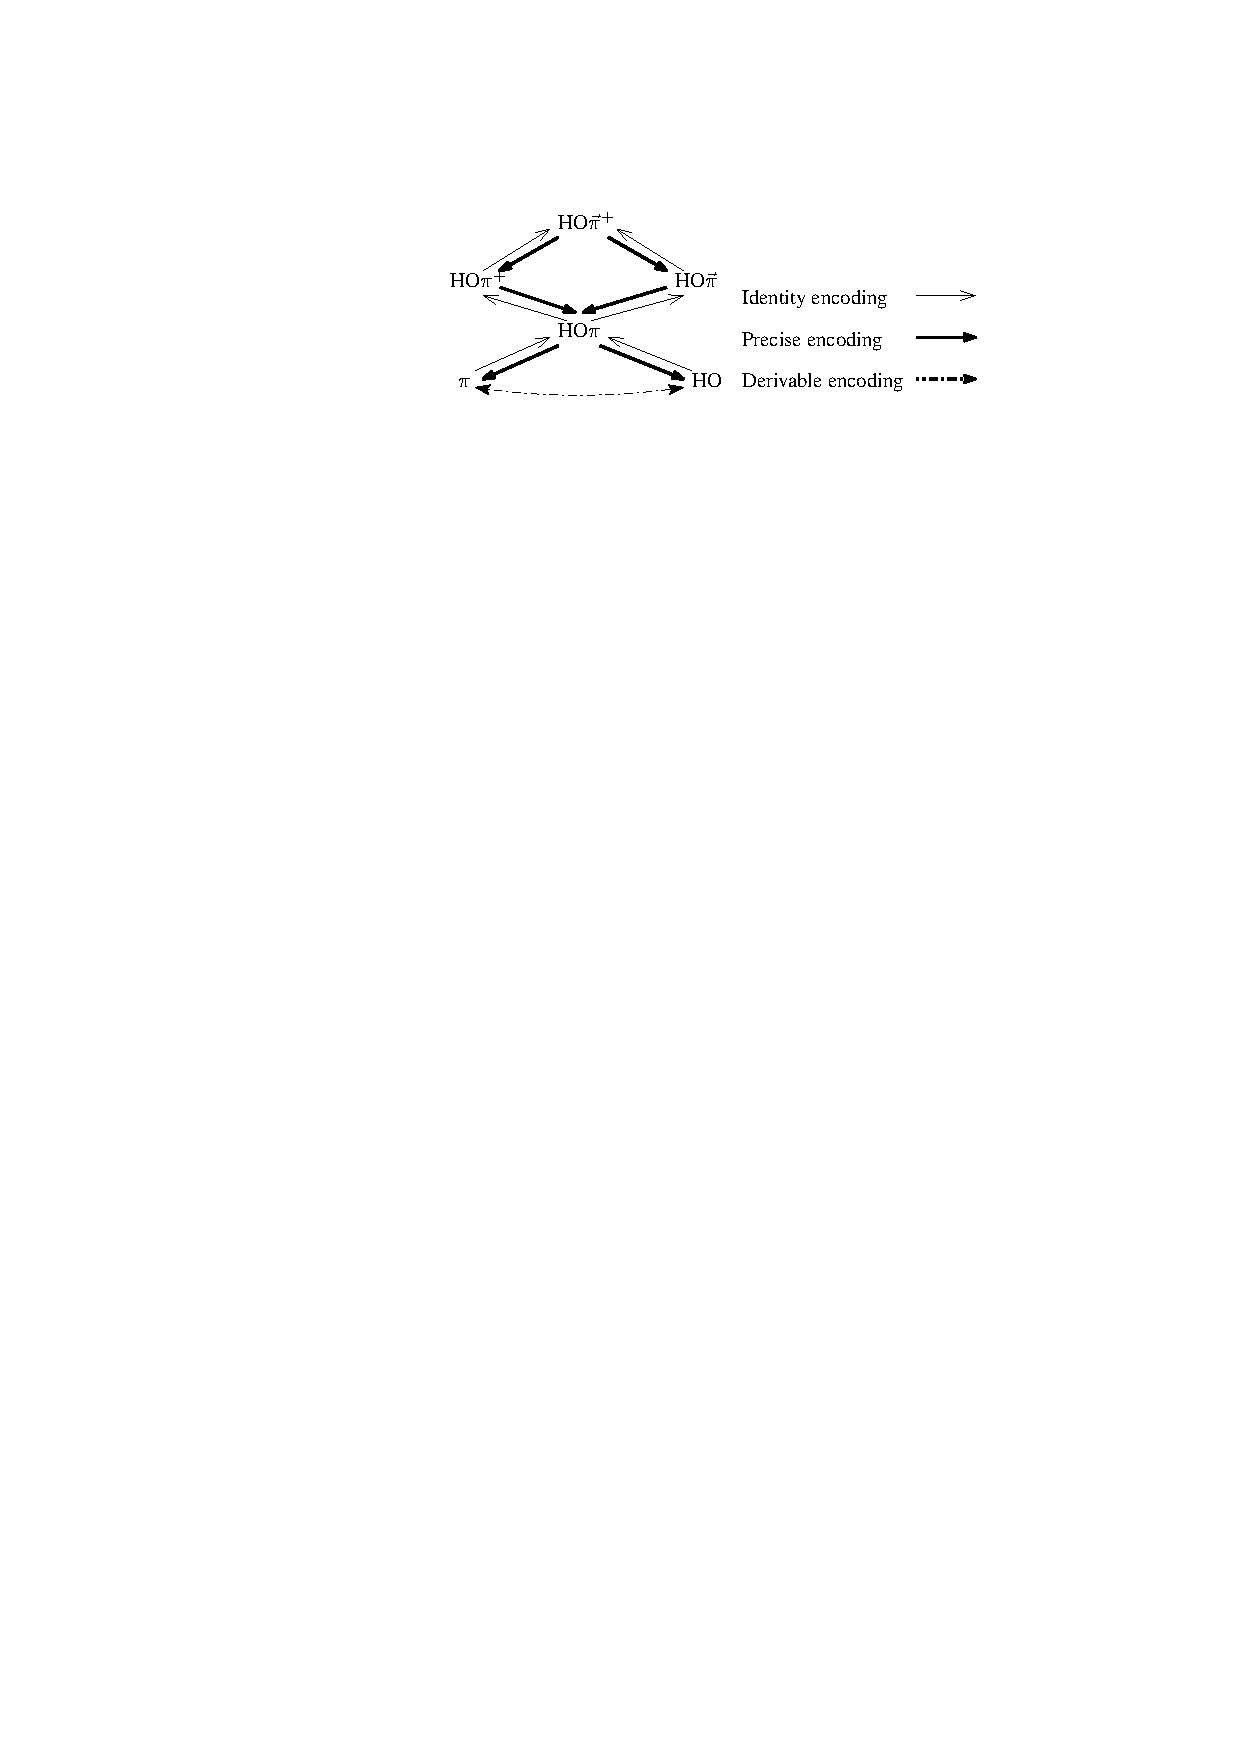
\includegraphics[scale=1]{diag.pdf}

	\caption{Encodability in Higher-Order Sessions. 
	Precise encodings are defined in \defref{def:goodenc}.
	\label{fig:express}}
\vspace{-5mm}
\Hlinefig
\end{figure}

\jparagraph{Context}
In \emph{session-based concurrency}, interactions are organized into \emph{sessions}, basic communication units.
Interaction patterns can then be abstracted as expressive \emph{session types}~\cite{honda.vasconcelos.kubo:language-primitives}, against which  specifications may be checked. 
%These patterns are defined as %(possibly recursive) 
%sequences of communication actions: % (send/receive a value, offer/select a behavior).
%For instance, 
%session type $T_1 = \btinp{\mathsf{str}} \btout{\mathsf{int}}  \tinact$ may be intuitively read as: receive (?) a value of type $\mathsf{str}$,then output (!) a value of type $\mathsf{int}$, finally close the protocol.
Session type $\btinp{U} S$ (resp.  $\btout{U} S$)
describes a protocol that first receives (resp. sends) a value of type $U$ and then continues as protocol $S$.
Also, given an index set $I$, types $\btbra{l_i:S_i}_{i \in I}$ 
and $\btsel{l_i:S_i}_{i \in I}$ 
define %, respectively,
%a branching and selection constructs for  
 a labeled choice mechanism; types 
$\trec{t}{S}$ 
and 
$\tinact$ denote recursive and completed protocols, respectively.
%describes a protocol that offers
%(resp. ) 
%Type $\tinact$ denotes the completed protocol.
In the (first-order) $\pi$-calculus~\cite{MilnerR:calmp1}, 
session types describe the intended interactive behavior of the names/channels in a process.
%names/channels are endowed with session types (such as $T_1$) representing their intended interactive behavior.

Session-based concurrency has also been casted in {higher-order} process
calculi which, by combining features from the $\lambda$-calculus and the $\pi$-calculus, 
enable the exchange of values 
that may contain processes~\cite{tlca07,DBLP:journals/jfp/GayV10}. 
%Higher-order calculi with sessions 
%naturally bridges concurrent and functional computation, 
%and enable the specification of protocols involving \emph{code mobility}, 
%commonplace in practice.
%The \HOp calculus enables 
%the specification of protocols involving \emph{code mobility}, 
%and includes
%Higher-order calculi with sessions 
The higher-order calculus with sessions studied here, denoted \HOp,
can specify protocols involving \emph{code mobility}: it includes
%equiped ping with 
constructs for 
synchronisation along shared names, 
session communication (value passing, labelled choice) along linear names,
recursion, 
 (first-order) abstractions 
 and applications.
 That is, 
 values in communications include names but also (first-order) abstractions---functions from name identifiers to processes. 
 %(In contrast, higher-order abstractions---functions from processes to processes---are disallowed.)
 (In contrast, we rule out higher-order abstractions---functions from processes to processes.)
Abstractions can be linear or shared; their types are  denoted $\lhot{C}$ and $\shot{C}$, respectively ($C$ 
%is a first-order type $C$ (say, a session name).
denotes a name). In \HOp we may have processes with a 
session type such as, e.g.,
%$T_2 = \btbra{upload:\btinp{\lhot{\mathsf{int}}}\tinact ~ , ~ sha:\btinp{\shot{\mathsf{int}}}\tinact}_{}$
$$S = \btbra{up:\btinp{\lhot{C}}\btout{\mathsf{ok}}\tinact ~ , ~ down:\btout{\shot{C}}\btout{\mathsf{ok}}\tinact ~ , ~quit:\btout{\mathsf{bye}}\tinact}_{}$$
that abstracts a server that offers different behaviors to clients: 
%  clients to select among distinct  behaviors: %namely, 
  to \emph{upload} a linear function, % (to be received by the server), 
  to \emph{download} a shared function, % (to be sent by the server),
   or to \emph{quit} the protocol. Subsequently, 
  the server sends a message ($\mathsf{ok}$ or $\mathsf{bye}$) before closing the session.


%\jparagraph{The Problem}
%%Roughly speaking, 
%  \HOp %, a higher-order process language that 
%extends Sangiorgi's higher-order $\pi$-calculus~\cite{SangiorgiD:expmpa} with session primitives.
%To be precise, %More precisely, 
%\HOp
%includes
%constructs for 
%%session establishment
%synchronisation along shared names, 
%session communication (value passing, labelled choice) along linear names,
%recursion, 
% (first-order) abstractions %(i.e., functions from name identifiers  to processes)
% and applications.
%% (denoted $\lambda x.P$ and $(\lambda x.P)a$, resp.).
%%While synchronization on shared names (useful to model session establishment) is 
%%non deterministic, session communication is deterministic and occurs on linear names.
%\HOp is therefore a rather rich language. This begs the question:
%%\begin{quote}
%is there a \emph{sub-calculus} of \HOp with equal expressivity? %hich is as expressive as the whole calculus? 
%%\end{quote}
%This question is of foundational interest, 
%for reasoning/validation techniques are more easily developed on small formalisms. 
%It also has practical ramifications, 
%as such a \emph{core calculus} could be taken as reference in 
%the design of %(functional) 
%programming languages with session types support.
%%implementations of languages with session primitives.
%Expressivity results may then help justifying useful connections 
%between foundational and practical advances on languages with concurrency and communication.
%
%%We have recently developed a behavioral theory  for \HOp~\cite{characteristic_bis}:
%%we introduced
%%\emph{characteristic bisimilarity}, a sound and complete 
%%characterization of contextual equivalence. % that enables tractable analyses.


\jparagraph{Expressiveness of \HOp}
%In this paper 
We study the type-preserving, 
relative expressivity of \HOp. % in relation. 
%to two 
%sub-calculi
%that distill first- and higher-order session-based concurrency. 
%\begin{enumerate}[-]
%\item 
As expected from 
known literature in the untyped setting \cite{SangiorgiD:expmpa}, 
the first-order session \sessp-calculus \jpc{(denoted~\sessp)} 
in~\cite{honda.vasconcelos.kubo:language-primitives} can encode  
\HOp preserving session types. 
%(\HOp without
%abstractions and applications) 
%\item 
In this paper, 
our \emph{main discovery} is 
that 
\HOp 
without
name-passing and recursion
can serve as a new core calculus    
for higher-order session concurrency.  
We call this core calculus \HO. 
We show that \HO can encode \HOp more efficiently 
than \sessp. In addition, in the higher-order session typed setting, 
\HO offers more tractable bisimulation techniques 
than \sessp. 
%constitute 
%the main sources 
%of expressivity in \HOp. 
%: \emph{name passing} and constructs for \emph{infinite behavior} (i.e., recursion and replication). 
%On the one hand, t
%Indeed, the expressivity of name-passing calculi (untyped/typed) is well known; e.g., the $\pi$-calculus can express 
%the $\lambda$-calculus and 
%process-passing calculi~\cite{SangiorgiD:expmpa}. 
%In the $\pi$-calculus, recursion and replication can be expressed in terms of each other. 
%On the other hand, 
%Higher-order concurrency is quite expressive too: 
%calculi without name passing and recursion are Turing equivalent~\cite{DBLP:journals/iandc/LanesePSS11}.
%Also, 
%recursion/replication operators are redundant in higher-order calculi: they can be represented using process passing and duplication~\cite{ThomsenB:plachoasgcfhop}. 

%\figref{fig:express} summarises %our expressivity 
%our encodability results. 


%While encoding \HOp 
%into the $\pi$-calculus preserving session types 
%(extending  known  results for untyped processes~\cite{SangiorgiD:expmpa}) is 
%%\jpc{already}
%significant, 



\jparagraph{Challenges and Contributions}

We assess the expressivity  of \HOp, \HO, and \sessp as delineated by session types. 
We introduce \emph{type-preserving encodings}:
we use type information to define process translations
and to retain the semantics of session protocols. 
Indeed,  not only we require 
well-typed source processes are encoded into 
well-typed target processes: 
we demand that session type constructs (input, output, branching, select) used to type the source process
are preserved by the typing of the target process.
This criterion is included in 
our notion of \emph{precise encoding} (\defref{def:goodenc}), which 
extends encodability criteria for untyped processes with 
\emph{full abstraction}.
{Full abstraction results are stated
up to two
behavioural equalities that characterise barbed congruence:
\emph{characteristic bisimilarity} ($\fwb$, defined in~\cite{characteristic_bis})
and 
\emph{higher-order bisimilarity} ($\hwb$), introduced in this
work.
It turns out that $\hwb$ offers more direct  reasoning than $\fwb$. }
Using precise encodings we establish strong correspondences between 
\HOp and its variants---see \figref{fig:express}. 



Our main contribution is 
an encoding of \HOp into \HO (\secref{subsec:HOpi_to_HO}).  
Since \HO lacks 
both name-passing and recursion, this encoding involves two \emph{key challenges}:
\begin{enumerate}[a.]
\item In known (typed) 
encodings of name-passing into process-passing~\cite{SaWabook} %are limited: % in that 
%they come with restrictions on name usages;  
%they 
%work for %name-passing 
%calculi 
%with \emph{capability types} 
%in which 
only the output capability of names can be sent---a received name cannot be used in later inputs.
This is far too limiting in \HOp, where 
 session names %denoting arbitrary protocols 
 may be passed around (\emph{delegation})
and types describe interaction  \emph{structures}, rather than ``loose'' name capabilities. % at a given time.



\item %As mentioned above, recursion % and replication)
%can be encoded in untyped higher-order calculi using process duplication. Unfortunately, this kind of encodings 
Known encodings of recursion in untyped higher-order calculi
do not carry over to session typed calculi such as \HOp,
because linear abstractions cannot be copied/duplicated. Hence, the discipline of session types  limits 
the possibilities for representing infinite behaviors---even simple forms, such as input-guarded replication.
\end{enumerate}




%MOTIVATION FIRST ENCODING (). \emph{Still to highlight: recursive type required, no recursion, small example.

%--- 
\noi
%We illustrate our approach. % to these challenges.
Our encoding overcomes these two obstacles, as we discuss in the following section.

Additional technical contributions include: 
(i)~the encodability of \HO into \sessp (\secref{subsec:HOp_to_sessp}); 
(ii)~extensions of our encodability results to richer settings (\secref{sec:extension});
(iii)~a non encodability result showing that shared names strictly add expressive power to session calculi (\secref{ss:negative}).
In essence, (i) extends known  results for untyped processes~\cite{SangiorgiD:expmpa} to the session typed setting.
Concerning (ii), we develop extensions of our encodings to 
\begin{enumerate}[-]
\item The extension of \HOp with \emph{higher-order} abstractions (\HOpp); 
\item The extension of \HOp with polyadic name passing and abstraction (\PHOp); 
\item The super-calculus of \HOpp and \PHOp (\PHOpp), equivalent to the calculus in~\cite{tlca07}.
\end{enumerate}
%\figref{fig:express} summarises %our expressivity 
%our encodability results. 
%From a global standpoint, our 
These
encodability results connect \HOp with existing higher-order process calculi~\cite{tlca07}, and  
further highlight the status of \HO as the core calculus for session concurrency.
Finally, although (iii) may be somewhat expected, to our knowledge we are the first to prove this separation result, 
exploiting session determinacy and typed equivalences.




\jparagraph{Outline} 
%This paper  is structured as follows.
%\begin{enumerate}[$\bullet$]
\secref{sec:overview} overviews key ideas of the precise encoding of \HOp into \sessp.
%\item 
\secref{sec:calculus} presents \HOp and its 
subcalculi (\HO and \sessp); %, and extensions (\HOpp and \PHOp).  
\secref{sec:types} summarizes their session type system.
\secref{sec:bt} presents  behavioral equalities for \HOp:
we recall definitions of barbed congruence and characteristic bisimilarity~\cite{characteristic_bis}, 
and introduce higher-order bisimilarity.
We show that these three typed relations coincide (\thmref{t:coincide}).
%and states type soundness 
%for \HOp and its variants.
\secref{s:expr} defines \emph{precise %(typed) 
encodings} by extending encodability criteria  for untyped processes. %~(e.g.,~\cite{DBLP:journals/iandc/Gorla10}).
%\item 
\secref{sec:positive} %and \S\,\ref{sec:negative}
gives {precise encodings} of \HOp into \HO and of \HOp into~\sessp (Thms.~\ref{f:enc:hopitoho} and~\ref{f:enc:hotopi}).
Mutual encodings between \sessp and \HO are derivable; 
all these calculi are thus equally expressive.
By means of empirical and formal comparisons between these two precise encodings, we establish that
\HOp and \HO are more tightly related than \HOp and \sessp (\thmref{t:tight}).
Moreover, we prove the impossibility of encoding communication along shared names
using linear names (\thmref{t:negative}).
%Exploiting determinacy and typed equivalences,
%\item
In \secref{sec:extension} %studies extensions of \HOp: 
we show that both \HOpp 
%(the extension with higher-order applications) 
and \PHOp 
%(the extension with polyadicity) 
are encodable in \HOp
(Thms.~\ref{f:enc:hopiptohopi} and \ref{f:enc:phopiptohopi}).
%This connects our work to the existing higher-order session calculus in~\cite{tlca07} (here denoted  $\PHOpp$).
%\item 
\secref{sec:relwork} collects concluding remarks and reviews related works.
%\secref{sec:concl} concludes.
The paper is self-contained. {\bf\em Omitted definitions and  proofs are in the Appendix and in~\cite{KouzapasPY15}.} 




\emph{Type-preserving compilations} are important in the design of
functional and object-oriented languages: type information has been
used to, e.g., justify code optimizations and reason about programs~\cite{DBLP:journals/toplas/MorrisettWCG99,DBLP:conf/pldi/ShaoA95,DBLP:journals/toplas/LeagueST02}.
A vast literature on 
{\em expressiveness} 
in concurrency theory
also studies compilations (or \emph{encodings})~\cite{Palamidessi03,DBLP:journals/iandc/Gorla10,DBLP:journals/tcs/FuL10,DBLP:conf/icalp/LanesePSS10,DBLP:journals/corr/PetersG15}:
they are used to transfer reasoning techniques 
%from one calculus to another, 
across calculi,
and to 
%identify constructs which may be implemented using simpler ones. 
implement programming abstractions using simple process constructs.
%To a large extent, however, this kind of \emph{expressiveness studies} concern only \emph{untyped process languages}.

In this work, we study 
{\em relative expressiveness} 
via \emph{type-preserving encodings} for \HOp, a \emph{higher-order} 
process language that integrates message-passing concurrency (including recursion) with functional features.
We consider source and target calculi coupled with \emph{session types}~\cite{honda.vasconcelos.kubo:language-primitives} denoting interaction protocols. 
Building on untyped frameworks for relative expressiveness
\cite{DBLP:journals/iandc/Gorla10}, 
we propose type preservation as a {new criterion} for \emph{precise encodings}.
We identify \HO, a new core calculus for higher-order session concurrency which lacks
name passing and recursion. 
We show that \HO can encode \HOp precisely and efficiently. 
Requiring  
type preservation makes
this encoding far from trivial: we crucially exploit advances on
session type duality~\cite{TGC14,DBLP:journals/corr/abs-1202-2086} and recent
characterisations of typed contextual equivalence \cite{characteristic_bis,KouzapasPY17}.
We develop a full hierarchy of variants of \HOp based on 
precise encodings: % (see \figref{fig:express}):
our encodings are
type-preserving and fully abstract up to typed
behavioural equalities. 
\newj{\figref{fig:express} illustrates this hierarchy; the variants of \HOp are explained next.}

\begin{figure}[t]
\centering
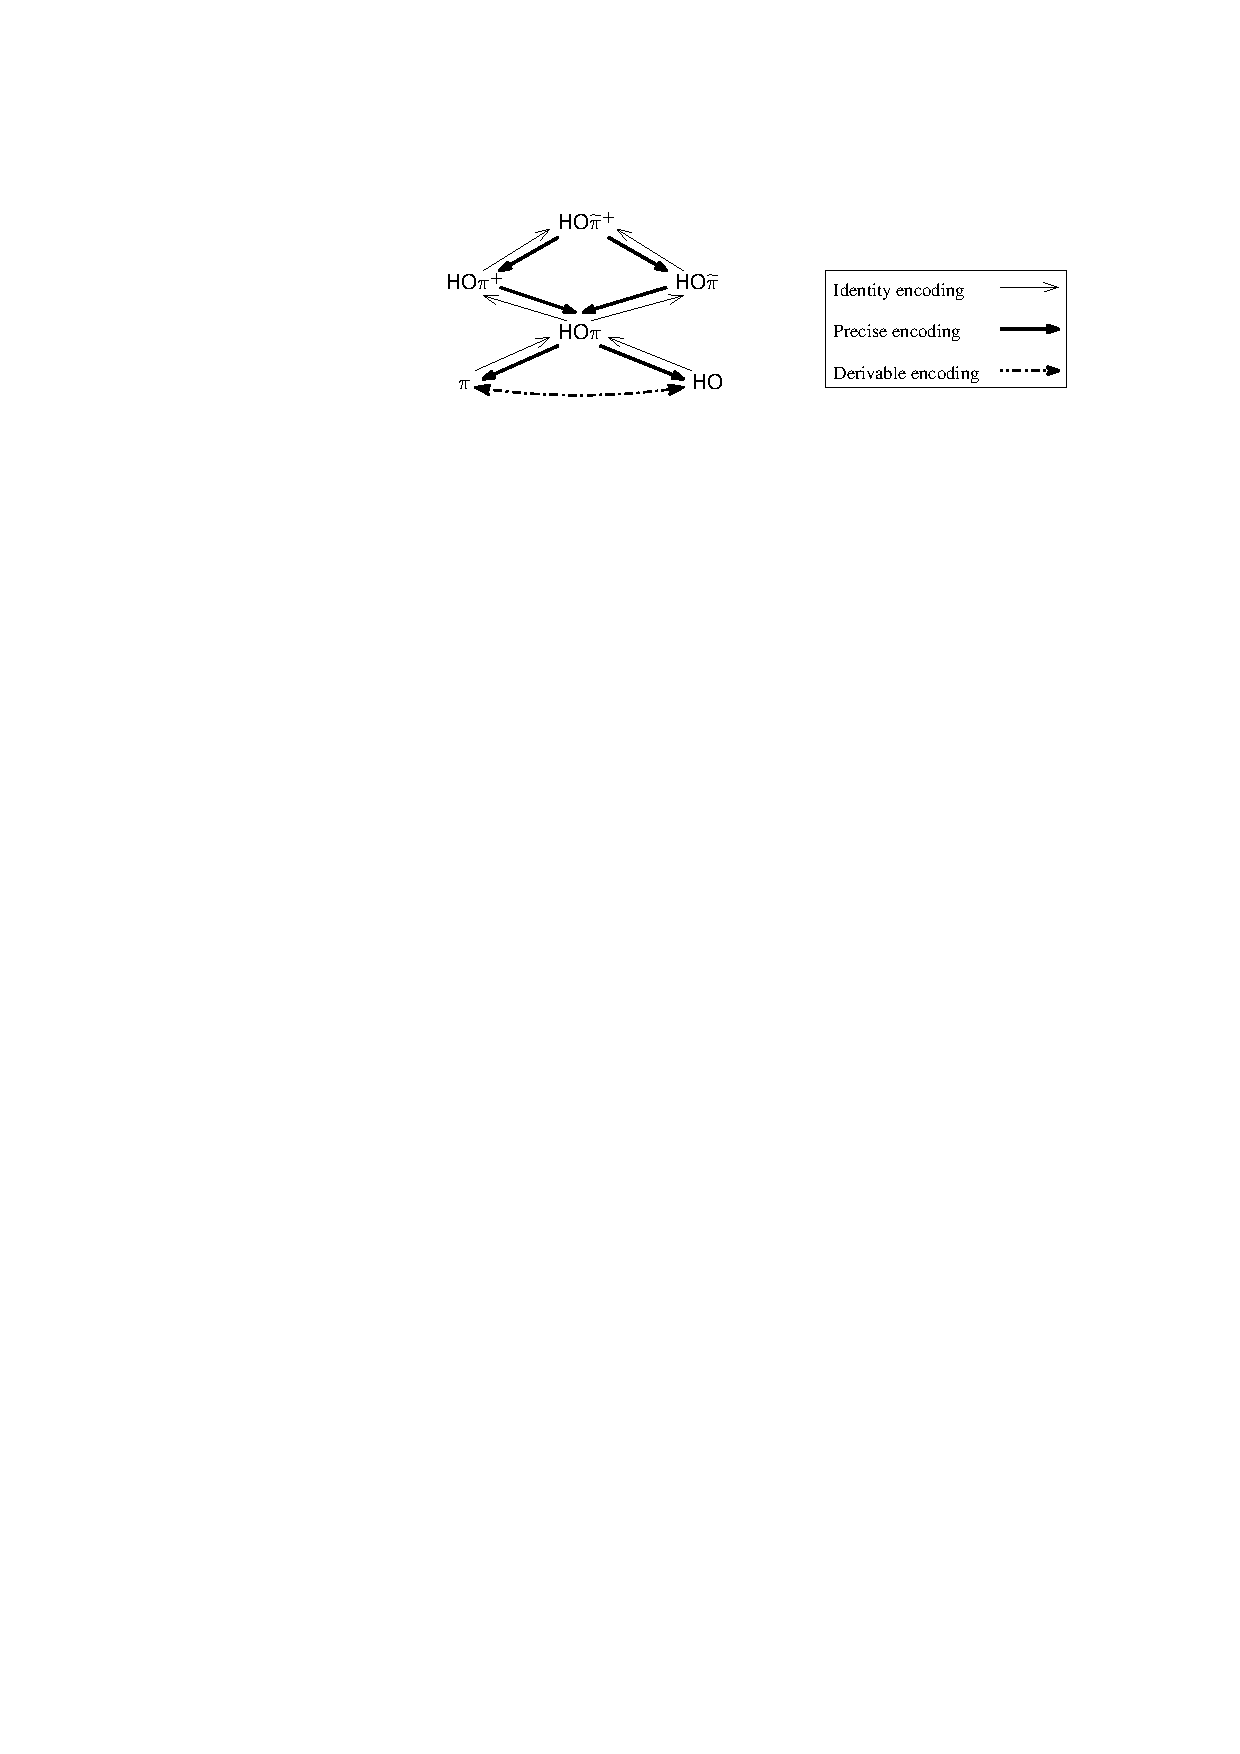
\includegraphics[scale=1]{./figures/diag.pdf}

	\caption{Encodability in Higher-Order Sessions. 
	Precise encodings are defined in \defref{def:goodenc}.
	\label{fig:express}}
%\vspace{-5mm}
%\Hlinefig
\end{figure}

\paragraph{Context}
In \emph{session-based concurrency}, interactions are organised into \emph{sessions}, basic communication units.
Interaction patterns can then be abstracted as \emph{session types}~\cite{honda.vasconcelos.kubo:language-primitives}, against which  specifications may be checked. 
%These patterns are defined as %(possibly recursive) 
%sequences of communication actions: % (send/receive a value, offer/select a behavior).
%For instance, 
%session type $T_1 = \btinp{\mathsf{str}} \btout{\mathsf{int}}  \tinact$ may be intuitively read as: receive (?) a value of type $\mathsf{str}$,then output (!) a value of type $\mathsf{int}$, finally close the protocol.
The session type $\btinp{U} S$ (resp.  $\btout{U} S$)
describes a protocol that first receives (resp. sends) a value of type $U$ and then continues as protocol $S$.
Also, given an index set $I$, types $\btbra{l_i:S_i}_{i \in I}$ 
and $\btsel{l_i:S_i}_{i \in I}$ 
define, %, respectively,
%a branching and selection constructs for  
\newj{respectively, external and internal choice constructs for}
 a labelled choice mechanism; types 
$\trec{t}{S}$ 
and 
$\tinact$ denote recursive and completed protocols, respectively.
%describes a protocol that offers
%(resp. ) 
%Type $\tinact$ denotes the completed protocol.
In the %(first-order) 
$\pi$-calculus, %~\cite{MilnerR:calmp1}, 
session types describe the intended interactive behaviour of the names %/channels 
in a process~\cite{honda.vasconcelos.kubo:language-primitives}.
%names/channels are endowed with session types (such as $T_1$) representing their intended interactive behavior.

%\end{document}

Session-based concurrency has also been casted in {higher-order} process
calculi which, by combining features from the $\lambda$-calculus and the $\pi$-calculus, 
enable the exchange of values 
that may contain processes~\cite{tlca07,DBLP:journals/jfp/GayV10}. 
%Higher-order calculi with sessions 
%naturally bridges concurrent and functional computation, 
%and enable the specification of protocols involving \emph{code mobility}, 
%commonplace in practice.
%The \HOp calculus enables 
%the specification of protocols involving \emph{code mobility}, 
%and includes
%Higher-order calculi with sessions 
The higher-order calculus with sessions studied here, called \HOp,
can specify protocols involving \emph{code mobility}: it includes
%equiped ping with 
constructs for 
synchronisation along shared names, 
session communication (value passing, labelled choice) along linear names,
recursion, 
 (first-order) abstractions 
 and applications.
 That is, 
 values in communications include names but also (first-order) abstractions---functions from name identifiers to processes. 
 %(In contrast, higher-order abstractions---functions from processes to processes---are disallowed.)
 (In contrast, \HOp lacks \emph{higher-order} abstractions---functions from processes to processes---but these can be encoded, see below.)
Abstractions can be linear or shared; their types are  denoted $\lhot{C}$ and $\shot{C}$, respectively ($C$ 
%is a first-order type $C$ (say, a session name).
denotes a name). 

%In \HOp we may have processes with a 
%session type such as, e.g.,
%%$T_2 = \btbra{upload:\btinp{\lhot{\mathsf{int}}}\tinact ~ , ~ sha:\btinp{\shot{\mathsf{int}}}\tinact}_{}$
%$$S = \btbra{{up}:\btinp{\lhot{C}}\btout{\mathsf{ok}}\tinact ~ , ~ {down}:\btout{\shot{C}}\btout{\mathsf{ok}}\tinact ~ , ~{quit}:\btout{\mathsf{bye}}\tinact}_{}\,.$$
%%that 
%$S$ is the type of 
%a server that offers ($\&$) \newj{three} different behaviours to a client: 
%%  clients to select among distinct  behaviors: %namely, 
%  to \emph{upload} a linear function, % (to be received by the server), 
%  to \emph{download} a shared function, % (to be sent by the server),
%   or to \emph{quit} the protocol. 
%   %Subsequently, 
%   \newj{Following a client's  selection ($\oplus$),}
%  the server sends a message ($\mathsf{ok}$ or $\mathsf{bye}$) before closing the session.





\paragraph{Expressiveness of \HOp}
%In this paper 
We study the type-preserving, 
relative expressivity of \HOp. % in relation. 
%to two 
%sub-calculi
%that distill first- and higher-order session-based concurrency. 
%\begin{enumerate}[-]
%\item 
As expected from 
known literature in the untyped setting \cite{SangiorgiD:expmpa}, 
the first-order session \sessp-calculus~\cite{honda.vasconcelos.kubo:language-primitives} {(here denoted~\sessp)} 
can encode  the higher-order calculus
\HOp preserving session types. 
%(\HOp without
%abstractions and applications) 
%\item 
In this paper, 
our {main discovery} 
concerns the opposite direction: we show 
that 
\HOp 
without
name-passing and recursion
%is a new 
can serve as a 
core calculus    
for higher-order session concurrency.  
We call this core calculus \HO. 
We show that \HO can encode \HOp more efficiently 
than \sessp. In addition, in the higher-order session typed setting, 
\HO offers more tractable bisimulation techniques 
than \sessp (cf. \secref{ss:equiv}).



\paragraph{Challenges and Contributions}

We assess the expressivity  of \HOp, \HO, and \sessp as delineated by session types. 
We introduce the notion of \emph{type-preserving encodings}:
type information is used to define encodings
and to retain the semantics of session protocols. 
Indeed,  not only we require 
well-typed source processes are encoded into 
well-typed target processes: 
we demand that session type constructs (input, output, branching, select) used to type the source process
are preserved by the typing of the target process.
This criterion is included in 
our notion of \emph{precise encoding} (\defref{def:goodenc}), which 
extends encodability criteria for untyped processes with 
\emph{full abstraction}.
{Full abstraction results are stated
up to two
behavioural equalities that characterise barbed congruence:
\emph{characteristic bisimilarity} ($\fwb$, introduced in~\cite{characteristic_bis})
and 
\emph{higher-order bisimilarity} ($\hwb$, introduced in~\cite{DBLP:conf/esop/KouzapasPY16} and  developed in~\cite{KouzapasPY17}).
%It turns out that $\hwb$ offers more direct  reasoning than $\fwb$. }
Using precise encodings we establish strong correspondences between 
\HOp and its variants---see 
%\figref{fig:express}. 
below.


Our contributions can be divided in two parts. 
First, we develop 
a precise encoding of \HOp into \HO (\secref{subsec:HOpi_to_HO}).  
Since \HO lacks 
both name-passing and recursion, this encoding involves two \emph{key challenges}:
\begin{enumerate}[a.]
\item In known (typed) 
encodings of name-passing into process-passing~\cite{SaWabook} %are limited: % in that 
%they come with restrictions on name usages;  
%they 
%work for %name-passing 
%calculi 
%with \emph{capability types} 
%in which 
only the output capability of names can be sent---a received name cannot be used in later inputs.
This is far too limiting in \HOp, where 
 session names %denoting arbitrary protocols 
 may be passed around (\emph{delegation})
and types describe interaction  \emph{structures}, rather than ``loose'' name capabilities. % at a given time.



\item %As mentioned above, recursion % and replication)
%can be encoded in untyped higher-order calculi using process duplication. Unfortunately, this kind of encodings 
Known encodings of recursion in untyped higher-order calculi
do not carry over to session typed calculi such as \HOp,
because linear abstractions cannot be copied/duplicated. Hence, the discipline of session types  limits 
the possibilities for representing infinite behaviours---this holds for even simple forms, such as input-guarded replication.
\end{enumerate}
\noindent Our encoding overcomes these two obstacles, as we discuss in \secref{sec:overview}.


In the second part, we offer additional technical contributions, which include: 
(i)~the encodability of \HO into \sessp (\secref{subsec:HOp_to_sessp}); 
(ii)~extensions of our encodability results to richer settings (\secref{sec:extension});
(iii)~a non encodability result showing that shared names strictly add expressive power to session calculi (\secref{ss:negative}).
In essence, (i) extends known  results for untyped processes~\cite{SangiorgiD:expmpa} to the session typed setting.
Concerning (ii), we develop extensions of our encodings to 
\begin{enumerate}[-]
\item The extension of \HOp with \emph{higher-order} abstractions (\HOpp); 
\item The extension of \HOp with polyadic name passing and abstraction (\PHOp); 
\item The super-calculus of \HOpp and \PHOp (denoted \PHOpp), equivalent to the calculus in~\cite{tlca07}.
\end{enumerate}
%\figref{fig:express} summarises %our expressivity 
%our encodability results. 
%From a global standpoint, our 

\newj{\figref{fig:express} summarises our encodability results: they}
%These encodability results 
connect \HOp with existing higher-order process calculi~\cite{tlca07}, and  
 highlight the status of \HO as the core calculus for session concurrency.
Finally, %although (iii) may be somewhat expected, 
to our knowledge we are the first to prove 
%this separation result, 
the non encodability result (iii),
exploiting session determinacy and typed equivalences.




\paragraph{Outline} 
%This paper  is structured as follows.
%\begin{enumerate}[$\bullet$]
\secref{sec:overview} overviews key ideas of the precise encoding of \HOp into \sessp.
%\item 
\secref{sec:prelim} 
collects background material:
\secref{subsec:syntax}
presents \HOp and its 
subcalculi (\HO and \sessp); %, and extensions (\HOpp and \PHOp).  
\secref{sec:types} summarises their session type system;
\secref{sec:bt}~pres\-ents  behavioural equalities for \HOp from~\cite{characteristic_bis,KouzapasPY17}:
barbed congruence, characteristic bisimilarity, 
and higher-order bisimilarity.
%We show that these three typed relations coincide (\thmref{t:coincide}).
%and states type soundness 
%for \HOp and its variants.
\secref{s:expr} defines \emph{precise %(typed) 
encodings} by extending encodability criteria  for untyped processes. %~(e.g.,~\cite{DBLP:journals/iandc/Gorla10}).
%\item 
\secref{sec:positive} %and \S\,\ref{sec:negative}
gives {precise encodings} of \HOp into \HO and of \HOp into~\sessp (Thms.~\ref{f:enc:hopitoho} and~\ref{f:enc:hotopi}).
Mutual encodings between \sessp and \HO are derivable; 
all these calculi are thus equally expressive.
%By means of 
Via
empirical and formal comparisons between these two precise encodings, in \secref{ss:compare} we establish that
\HOp and \HO are more tightly related than \HOp and \sessp (\thmref{t:tight}).
Moreover, we prove the impossibility of encoding communication along shared names
using linear names (\thmref{t:negative}).
%Exploiting determinacy and typed equivalences,
%\item
In \secref{sec:extension} %studies extensions of \HOp: 
we show 
%that both \HOpp 
%(the extension with higher-order applications) 
%and \PHOp 
%(the extension with polyadicity) 
%are encodable 
encodings of \HOpp and \PHOp 
into \HOp
(Thms.~\ref{f:enc:hoppptohop} and \ref{f:enc:phopiptohopi}).
%This connects our work to the existing higher-order session calculus in~\cite{tlca07} (here denoted  $\PHOpp$).
%\item 
\secref{sec:relwork} reviews related works and 
\secref{sec:concl} concludes.
%The paper is self-contained. 
{Omitted definitions and  proofs are in the Appendix.
% and  in~\cite{KouzapasPY15}.
} 

This paper is an extended and revised version of the homonymous conference paper that appeared in the Proceedings of ESOP'16~\cite{DBLP:conf/esop/KouzapasPY16}.
With respect to~\cite{DBLP:conf/esop/KouzapasPY16}, the current paper 
provides extended discussions, additional examples, and full technical details. 
Moreover, it offers a sharper focus on relative expressiveness:
a detailed treatment of higher-order bisimilarity
(first introduced in~\cite{DBLP:conf/esop/KouzapasPY16}) can now be found in our paper~\cite{KouzapasPY17} (which corresponds to the journal version of~\cite{characteristic_bis}).

%%%%%%%%%%%%%%%%%%%%%%%%%%%%%%%%%%%%%%%%%%%%%%%%%%%%%%%%%%%%%%%%%%%%%%%%%%%%%%%%
%%%%%%%%%%%%%%%%%%%%%%%%%%%%%%%%%%%%%%%%%%%%%%%%%%%%%%%%%%%%%%%%%%%%%%%%%%%%%%%%

\section{Overview: Encoding Name Passing Into Process Passing}
\label{sec:overview}
%% !TEX root = main.tex

\jparagraph{A Precise Encoding of Name-Passing into Process-Passing}
As mentioned above, 
our encoding of \HOp into \HO (\secref{subsec:HOpi_to_HO}) should 
%overcome two key challenges. First, it should 
(a)~enable the communication of arbitrary names, as required to represent delegation,
and 
%Second, it should 
(b)~address the fact that linearity of session types limits the 
possibilities for representing infinite behavior. 
To encode name passing into \HO 
%to encode name output, 
we ``pack''
the name to be sent into a suitable abstraction; 
upon reception, the receiver ``unpacks'' this object following a precise protocol on a fresh  session:
%More precisely, our encoding \jpc{of name passing} in \HO is given as:
\begin{center}
\begin{tabular}{rcll}
  $\map{\bout{a}{b} P}$	&$=$&	$\bout{a}{ \abs{z}{\,\binp{z}{x} (\appl{x}{b})} } \map{P}$ \\
  $\map{\binp{a}{x} Q}$	&$=$&	$\binp{a}{y} \newsp{s}{\appl{y}{s} \Par \bout{\dual{s}}{\abs{x}{\map{Q}}} \inact}$
\end{tabular}
\end{center}
%and as a homomorphism for the other operators.
Above, 
%where
$a,b$ are names and $s$ and $\dual{s}$ are 
linear session names (\emph{endpoints}).
%$\lambda x.P$ is a name abstraction of $P$; $\appl{x}{a}$ is a name application; 
Processes $\bout{a}{V} P$ and 
$\binp{a}{x} P$ denote output and input at~$a$;   
abstractions and applications are denoted
$\lambda x.P$ and $(\lambda x.P)a$; %, respectively;
$\newsp{s}P$ and $\inact$ represent hiding and inaction. %, respectively.
%Intuitively, the output of a name $b$ along name $a$ is encoded by
%the output of an abstraction containing $b$; the input of a name is encoded 
%by the input of an abstraction
Thus, following a communication on $a$, %our encoding features 
a (deterministic) reduction between  
$s$ and $\dual{s}$ guarantees that name $b$ is properly unpacked by means of abstraction passing
and appropriate applications.
Observe that 
\HO requires two extra reduction steps to mimic a name communication step in \HOp.
Also, it is worth stressing how an output action in the source process is translated into an output action in the encoded process (and similarly for input).
This is key to ensure the preservation of session type operators mentioned above (cf. \defref{def:tp}).

To preserve session linearity, we proceed as follows.
Given $\recp{X}{P}$, 
we encode the recursion body $P$ as an abstraction
in which free names of $P$ are converted into name variables.
%The encoding keeps track of these free names.
The resulting higher-order value is embedded in an input-guarded 
``duplicator'' process~\cite{ThomsenB:plachoasgcfhop}.
The recursion variable $X$ is then encoded 
in such a way that it
simulates recursion unfolding by 
invoking the duplicator in a by-need fashion.
That is, upon reception, the abstraction representing the 
recursion body $P$
is duplicated: 
one copy is used to reconstitute the original recursion body $P$ (through
the application of the free names of $P$); 
another copy is used to re-invoke the duplicator when needed. 
Interestingly, for this encoding to work 
we require non-tail recursive session types; to this end, 
we apply recent advances on the theory of duality for session types~\cite{TGC14,DBLP:journals/corr/abs-1202-2086}.

%To this end, we
%first record a mapping from recursive variable $X$ to process variable $z_X$.
%Then, we encode the recursion body $P$ as a name abstraction
%in which free names of $P$ are converted into name variables, using \defref{d:auxmap}.
%(Notice that $P$ is first encoded into \HO and then transformed using mapping
%$\auxmapp{\cdot}{{}}{\sigma}$.)
%Subsequently, this higher-order value is embedded in an input-guarded 
%``duplicator'' process~\cite{ThomsenB:plachoasgcfhop}. Finally, we define the encoding of $X$ 
%in such a way that it
%simulates recursion unfolding by 
%invoking the duplicator in a by-need fashion.
%That is, upon reception, the \HO abstraction which encodes  the 
%recursion body $P$
%%containing $\auxmapp{P}{{}}{\sigma}$ 
%is duplicated: 
%one copy is used to reconstitute the original recursion body $P$ (through
%the application of $\fn{P}$); another copy is used to re-invoke
%the duplicator when needed. 
%
%We encode recursion with non-tail recursive session types; for this 
%we apply recent advances on the theory of session duality~\cite{TGC14,DBLP:journals/corr/abs-1202-2086}.

\jparagraph{A Plausible Encoding That is Not Precise}
Our notion of \emph{precise encoding} (\secref{s:expr}) that
requires the translation of both process and types, and 
admits only process mappings that preserve session types
\emph{and} are fully abstract. Thus, our encodings 
not only exhibit  strong behavioral correspondences, but also 
 relate source and target processes with  
communication structures described by session types.
%Moreover, the notion of encoding includes full abstraction as encodability criteria.
These strict requirements make our developments far from trivial.
In particular, requiring type preservation rules out other plausible encoding strategies.
To illustrate this point,
consider the  following encoding of %$\sessp$ 
name-passing 
into $\HO$:\footnote{This alternative  encoding was suggested by an anonymous reviewer of a previous version of this paper.} %defined as
\begin{center}
\begin{tabular}{rcll}
  $\umap{\bout{a}{b} P}$	&$=$&	$\binp{a}{x}( \appl{x}{b} \Par \umap{P})$ \\
  $\umap{\binp{a}{x} Q}$	&$=$&	$\bout{a}{\abs{x}{\umap{Q}}} \inact$
\end{tabular}
\end{center}
%and as a homomorphism for the other operators.
Intuitively, 
rather than sending a package with name $b$, 
this encoding sends the continuation of the input. Observe how this mapping entails  a 
``role inversion'': outputs are translated into inputs, and inputs are translated into outputs. 
Although perfectly reasonable, the encoding $\umap{\cdot}$  
%is far from desirable in a session typed setting: 
is \emph{not type preserving}. Consequently, it is also not \emph{precise}.
%Type preservation is intended to preserve the overall semantics of session types:
Since individual prefixes (input, output, branching, select) 
represent actions in a structured communication sequence (i.e., a protocol abstracted by a session type),
the encoding above would simply alter the meaning of the session protocol in the source language.





\paragraph{A Precise Encoding of Name-Passing into Process-Passing}
As mentioned above, 
our encoding of \HOp into \HO (\secref{subsec:HOpi_to_HO}) should 
%overcome two key challenges. First, it should 
(a)~enable the communication of arbitrary names, as required to represent delegation,
and 
%Second, it should 
(b)~address the fact that linearity as enforced by session types limits the 
possibilities for representing infinite behaviour. 

To illustrate our encoding of name passing into \HO, we informally introduce some process syntax; formal definitions are given in \secref{subsec:syntax}.
Below, 
$a,b$ are names and $s$ and $\dual{s}$ are 
linear session names (\emph{endpoints}).
%$\lambda x.P$ is a name abstraction of $P$; $\appl{x}{a}$ is a name application; 
Processes $\bout{a}{V} P$ and 
$\binp{a}{x} P$ denote output and input at~$a$, respectively;   
abstractions and applications are denoted
$\lambda x.P$ and $(\lambda x.P)a$, respectively. 
Processes %, respectively;
$\newsp{s}P$, $P \Par Q$, and $\inact$ represent usual forms of name restriction/hiding, parallel composition, and inaction. 

In our encoding, 
%to encode name output, 
we ``pack''
the name to be sent into an abstraction; 
upon reception, the receiver ``unpacks'' this object following a precise protocol on a fresh  session:
%More precisely, our encoding \jpc{of name passing} in \HO is given as:
\begin{align*}
  \map{\bout{a}{b} P}	&= \bout{a}{ \abs{z}{\,\binp{z}{x} (\appl{x}{b})} } \map{P} \\
  \map{\binp{a}{x} Q}	&=	 \binp{a}{y} \newsp{s}{\appl{y}{s} \Par \bout{\dual{s}}{\abs{x}{\map{Q}}} \inact}
\end{align*}
%and as a homomorphism for the other operators.
%, respectively.
%Intuitively, the output of a name $b$ along name $a$ is encoded by
%the output of an abstraction containing $b$; the input of a name is encoded 
%by the input of an abstraction
Thus, 
an abstraction containing the name $b$ is first passed around along $a$.
Following this communication, %our encoding features 
a sequence of (deterministic) reductions between  
$s$ and $\dual{s}$ guarantees that $b$ is properly unpacked by means of abstraction passing
and appropriate applications.
Indeed, 
%\HO 
\newjb{the above encoding}
requires %two 
\newjb{three}
extra reduction steps to mimic a single name communication step in \HOp.
Also, notice that an output action in the source process is translated into an output action in the encoded process (and similarly for input).
This is key to ensure the preservation of session type operators mentioned above (cf. \defref{def:tp}).

\newj{As hinted at above, 
a challenge in 
 encoding $\recp{X}{P}$ is  
preserving linearity  of session names.
Intuitively, we encode the recursion body $P$ as an abstraction 
$\abs{\tilde{x}}{\auxmapp{P}{{}}{\sigma}}$
in which each session name of $P$ (included in 
set $\sigma$)
is converted into a name variable in $\tilde{x}$.
Since  
$\abs{\tilde{x}}{\auxmapp{P}{{}}{\sigma}}$
does not mention (linear) session names,
we may embed it into a 
``duplicator'' process
which implements recursion using higher-order communication~\cite{ThomsenB:plachoasgcfhop}. 
The encoding of the recursion variable $X$
invokes this duplicator in a by-need fashion:
it receives 
$\abs{\tilde{x}}{\auxmapp{P}{{}}{\sigma}}$ and uses two copies of it:
one copy allows us to obtain $P$
through the application of the session names of $P$; 
the other allows us
to invoke the duplicator when needed. 
Interestingly, for this encoding to work 
we require non-tail recursive session types; 
this exploits recent advances on the theory of duality for session types~\cite{TGC14,DBLP:journals/corr/abs-1202-2086}.}


%To preserve session linearity, we proceed as follows.
%Given $\recp{X}{P}$, 
%we encode the recursion body $P$ as an abstraction
%in which free names of $P$ are converted into name variables.
%The resulting higher-order value is embedded in an input-guarded 
%``duplicator'' process~\cite{ThomsenB:plachoasgcfhop}.
%The recursion variable $X$ is then encoded 
%in such a way that it
%simulates recursion unfolding by 
%invoking the duplicator in a by-need fashion.
%That is, upon reception, the abstraction representing the 
%recursion body $P$
%is duplicated: 
%one copy is used to reconstitute the original recursion body $P$ (through
%the application of the free names of $P$); 
%another copy is used to re-invoke the duplicator when needed. 
%Interestingly, for this encoding to work 
%we require non-tail recursive session types; to this end, 
%we apply recent advances on the theory of duality for session types~\cite{TGC14,DBLP:journals/corr/abs-1202-2086}.

%To this end, we
%first record a mapping from recursive variable $X$ to process variable $z_X$.
%Then, we encode the recursion body $P$ as a name abstraction
%in which free names of $P$ are converted into name variables, using \defref{d:auxmap}.
%(Notice that $P$ is first encoded into \HO and then transformed using mapping
%$\auxmapp{\cdot}{{}}{\sigma}$.)
%Subsequently, this higher-order value is embedded in an input-guarded 
%``duplicator'' process~\cite{ThomsenB:plachoasgcfhop}. Finally, we define the encoding of $X$ 
%in such a way that it
%simulates recursion unfolding by 
%invoking the duplicator in a by-need fashion.
%That is, upon reception, the \HO abstraction which encodes  the 
%recursion body $P$
%%containing $\auxmapp{P}{{}}{\sigma}$ 
%is duplicated: 
%one copy is used to reconstitute the original recursion body $P$ (through
%the application of $\fn{P}$); another copy is used to re-invoke
%the duplicator when needed. 
%
%We encode recursion with non-tail recursive session types; for this 
%we apply recent advances on the theory of session duality~\cite{TGC14,DBLP:journals/corr/abs-1202-2086}.

\paragraph{A Plausible Encoding That is Not Precise}
Our notion of \emph{precise encoding} (\defref{def:goodenc}) 
requires the translation of both process and types; it  
admits only process mappings that preserve session types
\emph{and} are fully abstract. Thus, our encodings 
not only exhibit  strong behavioural correspondences, but also 
 relate source and target processes with consistent 
communication structures described by session types.
%Moreover, the notion of encoding includes full abstraction as encodability criteria.
These requirements are demanding and make our developments far from trivial.
In particular, requiring type preservation may rule out other plausible encoding strategies.
To illustrate this point,
consider the  following \newjb{alternative} encoding of %$\sessp$ 
name-passing 
into $\HO$:\footnote{This encoding was suggested by a reviewer of a previous version of this paper.} %defined as
\begin{align*}
   \umap{\binp{a}{x} Q} & = \bout{a}{\abs{x}{\umap{Q}}} \inact \\
     \umap{\bout{a}{b} P} 	&= \binp{a}{x}( \appl{x}{b} \Par \umap{P})
\end{align*}
%and as a homomorphism for the other operators.
{Intuitively, 
the encoding of input takes the initiative by sending an abstraction containing the encoding of its continuation $Q$;
the encoding of output applies this received value to name $b$.}
%rather than sending a package with name $b$, this encoding sends the continuation of the input. 
Hence, this mapping entails  a 
``role inversion'': outputs are translated into inputs, and inputs are translated into outputs. 
Although fairly reasonable, we will see that the encoding $\umap{\cdot}$  
%is far from desirable in a session typed setting: 
is \emph{not type preserving}. Consequently, it is also not \emph{precise}.
%Type preservation is intended to preserve the overall semantics of session types:
Since individual prefixes (input, output, branching, select) 
represent actions in a structured communication sequence (i.e., a protocol abstracted by a session type),
the encoding~$\umap{\cdot}$ would simply alter the meaning of the session protocol in the source language.

%%%%%%%%%%%%%%%%%%%%%%%%%%%%%%%%%%%%%%%%%%%%%%%%%%%%%%%%%%%%%%%%%%%%%%%%%%%%%%%%
%%%%%%%%%%%%%%%%%%%%%%%%%%%%%%%%%%%%%%%%%%%%%%%%%%%%%%%%%%%%%%%%%%%%%%%%%%%%%%%%

%% !TEX root = main.tex
\section{Higher-Order Session $\pi$-Calculi}
\label{sec:calculus}

We introduce 
the \emph{higher-order session $\pi$-calculus} (\HOp).
We define 
syntax, operational semantics, and 
its sub-calculi (\sessp and \HO).
In the following sections we will introduce 
type system,
behavioral equivalences, 
 and extensions of \HOp (\HOpp and \PHOp). 


%We also introduce two subcalculi of \HOp. In particular, we define the 
%core higher-order session
%calculus (\HO), which 
%%. The \HO calculus is  minimal: it 
%includes constructs for shared name synchronisation and 
%%constructs for session establish\-ment/communication and 
%(monadic) name-abstraction, but lacks name-passing and recursion.

%Although minimal, in \secref{s:expr}
%the abstraction-passing capabilities of \HOp will prove 
%expressive enough to capture key features of session communication, 
%such as delegation and recursion.

\subsection{\HOp: Syntax, Operational Semantics, Subcalculi}
\label{subsec:syntax}

\jparagraph{Syntax}
The syntax of \HOp is defined in \figref{fig:syntax}.
\HOp it is a subcalculus of the language studied 
in~\cite{tlca07}. It is also a variant of the language that we investigated in~\cite{characteristic_bis}, 
where higher-order value applications were considered. 


% !TEX root = ../journal16kpy.tex
	\begin{figure}[t]
		\begin{align*}
			n  & \bnfis a,b \bnfbar s, \dual{s} 
			\\
			u,w  & \bnfis n \bnfbar x,y,z 
			\\
			V,W  & \bnfis \nonhosyntax{u} \bnfbar \nonpisyntax{\abs{x}{P}}
			\\[1mm]
			P,Q
			 & \bnfis 
			\bout{u}{V}{P}  \sbnfbar  \binp{u}{x}{P} \sbnfbar
			\bsel{u}{l} P \sbnfbar \bbra{u}{l_i:P_i}_{i \in I} \sbnfbar \nonpisyntax{\appl{V}{u}}
			\\[1mm]
			 & \sbnfbar P\Par Q \sbnfbar \news{n} P 
			\sbnfbar \inact \sbnfbar \nonhosyntax{\rvar{X} \sbnfbar \recp{X}{P}}
%			\\%[1mm]
%			 \bnfbar &
%			\nonhosyntax{\rvar{X} \bnfbar \recp{X}{P}}
		\end{align*}
	\caption{\newjb{Syntax of \HOp. While \HO lacks \nonhosyntax{\text{shaded}} constructs, \sessp lacks \nonpisyntax{\text{boxed}} constructs.}}
	\label{fig:syntax}
%	\vspace{-1mm}
%	\Hlinefig
\end{figure}



%\myparagraph{Values}
\emph{Names} $a,b,c, \dots$ (resp.~$s, \dual{s}, \dots$) 
range over shared (resp. session) names. 
Names $m, n, t, \dots$ are session or shared names.
Dual endpoints are $\dual{n}$ with
$\dual{\dual{s}} = s$ and $\dual{a} = a$.
%We define the dual operation over names $n$ as $\dual{n}$ with
%$\dual{\dual{s}} = s$ and $\dual{a} = a$.
%Intuitively, names $s$ and $\dual{s}$ are dual (two) \emph{endpoints} while 
%shared names represent shared (non-deterministic) points. 
Variables are denoted with $x, y, z, \dots$, 
and recursive variables are denoted with $\varp{X}, \varp{Y} \dots$.
An abstraction %(or higher-order value) 
$\abs{x}{P}$ is a process $P$ with name parameter $x$.
%Symbols $u, v, \dots$ range over identifiers; and  $V, W, \dots$ to denote values. 
\emph{Values} $V,W$ include 
identifiers $u, v, \ldots$ %(first-order values) 
and 
abstractions $\abs{x}{P}$ (first- and higher-order values, resp.). 

%\myparagraph{Terms} 

Terms
include the
$\pi$-calculus prefixes for sending and receiving values $V$.
%Process $\bout{u}{V} P$ denotes the output of value $V$
%over name $u$, with continuation $P$;
%process $\binp{u}{x} P$ denotes the input prefix on name $u$ of a value
%that 
%will substitute variable $x$ in continuation $P$. 
Recursion is expressed by $\recp{X}{P}$,
which binds the recursive variable $\varp{X}$ in process $P$.
Process 
%ny
%$\appl{x}{u}$ 
$\appl{V}{u}$ 
is the application
which substitutes name $u$ on the abstraction~$V$. 
Typing  ensures that $V$ is not a name.
Processes $\bsel{u}{l} P$ and $\bbra{u}{l_i: P_i}_{i \in I}$ are the
standard session processes for selecting and branching.
%Prefix $\bsel{u}{l} P$ selects label $l$ on name $u$ and then behaves as $P$.
%Given $i \in I$ 
%Process $\bbra{u}{l_i: P_i}_{i \in I}$ offers a choice on labels $l_i$ with
%continuation $P_i$, given that $i \in I$.
%Others are standard c
Constructs for 
inaction $\inact$,  parallel composition $P_1 \Par P_2$, and 
name restriction $\news{n} P$ are standard.
Session name restriction $\news{s} P$ simultaneously binds endpoints $s$ and $\dual{s}$ in $P$.
%A well-formed process relies on assumptions for
%guarded recursive processes.
Functions $\fv{P}$ and $\fn{P}$ denotet the sets of free 
%\jpc{recursion}
variables and names; 
and assume $V$ in $\bout{u}{V}{P}$ does not include free recursive 
variables $\rvar{X}$.
If $\fv{P} = \emptyset$, we call $P$ {\em closed}.
%; and closed $P$ without 
%free session names a {\em program}. 




%\subsection{Operational Semantics}
%\label{subsec:semantics}


\jparagraph{Operational Semantics}
The \emph{operational semantics} of \HOp is defined in terms of a reduction relation, 
denoted $\red$ and 
given in 
 \figref{fig:reduction} (top).
 We briefly explain the rules. 
Rule $\orule{App}$ defines  name application.
Rule $\orule{Pass}$ defines a shared interaction at $n$ 
(with $\dual{n}=n$) or a session interaction.
Rule $\orule{Sel}$ is the standard rule for labelled choice/selection.%:
%given an index set $I$, 
%a process selects label $l_j$ on name $n$ over a set of
%labels $\set{l_i}_{i \in I}$ offered by a branching 
%on the dual endpoint $\dual{n}$;
Other rules are standard $\pi$-calculus rules.
Reduction is closed under \emph{structural congruence} as defined in \figref{fig:reduction} (bottom). 
We assume the expected extension of $\scong$ to values $V$.
We write $\red^\ast$ for a multi-step reduction.

\begin{figure}[!t]
\[
	\begin{array}{rcllcrcll}
%	\begin{array}{c}
		\appl{(\abs{x}{P})}{u}  & \red & P \subst{u}{x} 
		& \orule{App}
%		\\[1mm]
		&&
		\bout{n}{V} P \Par \binp{\dual{n}}{x} Q & \red & P \Par Q \subst{V}{x} 
		& \orule{Pass}
		\\[1mm]

		\bsel{n}{l_j} Q \Par \bbra{\dual{n}}{l_i : P_i}_{i \in I} & \red & Q \Par P_j ~~(j \in I)~~ 
		& \orule{Sel}
%		\\[1mm]
		&&
		P \red P'\Rightarrow  \news{n} P   & \red  &  \news{n} P' 
		& \orule{Res}
		\\[1mm]

		P \red P' & \Rightarrow  &  P \Par Q  \red   P' \Par Q  
		& \orule{Par}
%		\\[1mm]
		&&
		P \scong Q \red Q' \scong P' & \Rightarrow & P  \red  P'
		& \orule{Cong}
	\end{array}
\]
{\small
\[
	\begin{array}{c}
		P \Par \inact \scong P
		\quad
		P_1 \Par P_2 \scong P_2 \Par P_1
		\quad
		P_1 \Par (P_2 \Par P_3) \scong (P_1 \Par P_2) \Par P_3
%		\\[1mm]
		\quad
		\news{n} \inact \scong \inact
%		\quad 
		\\[1mm]
		P \Par \news{n} Q \scong \news{n}(P \Par Q)
		\ (n \notin \fn{P})
		\quad 
		\recp{X}{P} \scong P\subst{\recp{X}{P}}{\rvar{X}}
%		\\[1mm]
		\quad
		P \scong Q \textrm{ if } P \scong_\alpha Q
%		\qquad
%		\dk{V \scong W \textrm{ if } V \scong_\alpha W
%\quad \abs{x}{P} \scong \abs{x}{Q} \textrm{ if } P \scong Q}
	\end{array}
\]
}
%\vspace{-3mm}
\caption{Operational Semantics of $\HOp$. 
%\vspace{-1mm}
\label{fig:reduction}}
%\Hlinefig
\end{figure}



\jparagraph{Subcalculi}
%\label{subsec:subcalculi}
\noi As motivated in the introduction, 
we define two \emph{subcalculi} of \HOp. 
%We now define several sub-calculi of \HOp. 
\begin{enumerate}[$\bullet$]
	\item	The  
		{\em core higher-order session calculus} (denoted \HO),
		 lacks recursion and name passing; its 
		formal syntax is obtained from \figref{fig:syntax} by excluding 
		constructs in \nonhosyntax{\text{grey}}.

	\item	The   
		the {\em session $\pi$-calculus} 
		(denoted $\sessp$), which 
		lacks  the
		higher-order constructs
		(i.e., abstraction passing and application), but includes recursion.

%	\item	The third sub-calculus, denoted \haskp, represents cloud Haskell:
%		\[
%			\begin{array}{rclllll}
%				V,W	& ::= &		u \bnfbar  \abs{x}{P}
%				\\
%				P,Q	& ::= &		\bout{u}{m}{P}  \bnfbar  \binp{u}{x}{P} \bnfbar
%							\bsel{u}{l} P \bnfbar \bbra{u}{l_i:P_i}_{i \in I}
%				\\[1mm]
%					& \bnfbar &	\appl{V}{V} \bnfbar P\Par Q \bnfbar \news{n} P \bnfbar \inact
%		\end{array}
%		\]
\end{enumerate}
%
Let $\CAL \in \{\HOp, \HO, \sessp\}$. We write 
$\CAL^{-\mathsf{sh}}$ for $\CAL$ without shared names
(we delete $a,b$ from $n$). 
We shall demonstrate in Section~\ref{sec:positive} that 
$\HOp$, $\HO$, and $\sessp$ have the same expressivity.


%\section{Higher-Order Session $\pi$-Calculi}
\section{Preliminaries}
\label{sec:prelim}

We introduce 
the \emph{higher-order session $\pi$-calculus} (\HOp).
We first define 
syntax, operational semantics, and 
its sub-calculi (\sessp and \HO).
Then, a type system and behavioural equivalences for \HOp are recalled in 
\secref{sec:types} and \secref{sec:bt}. 
\HOp features first-order abstractions and monadic communication; extensions 
with higher-order abstractions and polyadicity (noted \HOpp and \PHOp, respectively) 
are discussed in \secref{sec:extension}.


%We also introduce two subcalculi of \HOp. In particular, we define the 
%core higher-order session
%calculus (\HO), which 
%%. The \HO calculus is  minimal: it 
%includes constructs for shared name synchronisation and 
%%constructs for session establish\-ment/communication and 
%(monadic) name-abstraction, but lacks name-passing and recursion.

%Although minimal, in \secref{s:expr}
%the abstraction-passing capabilities of \HOp will prove 
%expressive enough to capture key features of session communication, 
%such as delegation and recursion.

\subsection{\HOp: Syntax, Operational Semantics, and Subcalculi}
\label{subsec:syntax}

\paragraph{Syntax}
The syntax of \HOp is defined in \figref{fig:syntax}.
\HOp  is a subcalculus of the language studied 
in~\cite{tlca07}. It is also a variant of the language that we investigated in~\cite{characteristic_bis}, 
which includes higher-order value applications. 


% !TEX root = ../journal16kpy.tex
	\begin{figure}[t]
		\begin{align*}
			n  & \bnfis a,b \bnfbar s, \dual{s} 
			\\
			u,w  & \bnfis n \bnfbar x,y,z 
			\\
			V,W  & \bnfis \nonhosyntax{u} \bnfbar \nonpisyntax{\abs{x}{P}}
			\\[1mm]
			P,Q
			 & \bnfis 
			\bout{u}{V}{P}  \sbnfbar  \binp{u}{x}{P} \sbnfbar
			\bsel{u}{l} P \sbnfbar \bbra{u}{l_i:P_i}_{i \in I} \sbnfbar \nonpisyntax{\appl{V}{u}}
			\\[1mm]
			 & \sbnfbar P\Par Q \sbnfbar \news{n} P 
			\sbnfbar \inact \sbnfbar \nonhosyntax{\rvar{X} \sbnfbar \recp{X}{P}}
%			\\%[1mm]
%			 \bnfbar &
%			\nonhosyntax{\rvar{X} \bnfbar \recp{X}{P}}
		\end{align*}
	\caption{\newjb{Syntax of \HOp. While \HO lacks \nonhosyntax{\text{shaded}} constructs, \sessp lacks \nonpisyntax{\text{boxed}} constructs.}}
	\label{fig:syntax}
%	\vspace{-1mm}
%	\Hlinefig
\end{figure}



%\myparagraph{Values}
\emph{Names} $a,b,c, \dots$ (resp.~$s, \dual{s}, \dots$) 
range over shared (resp. session) names. 
Names $m, n, t, \dots$ are session or shared names.
Dual endpoints are $\dual{n}$ with
$\dual{\dual{s}} = s$ and $\dual{a} = a$.
%We define the dual operation over names $n$ as $\dual{n}$ with
%$\dual{\dual{s}} = s$ and $\dual{a} = a$.
%Intuitively, names $s$ and $\dual{s}$ are dual (two) \emph{endpoints} while 
%shared names represent shared (non-deterministic) points. 
Variables are denoted with $x, y, z, \dots$, 
and recursive variables are denoted with $\varp{X}, \varp{Y} \dots$.
An abstraction %(or higher-order value) 
$\abs{x}{P}$ is a process $P$ with name parameter $x$.
%Symbols $u, v, \dots$ range over identifiers; and  $V, W, \dots$ to denote values. 
\emph{Values} $V,W, \ldots$ include 
identifiers $u, v, \ldots$ %(first-order values) 
and 
abstractions $\abs{x}{P}$ (first- and higher-order values, resp.). 

%\myparagraph{Terms} 

Process terms $P, Q, \ldots$ 
include usual %$\pi$-calculus 
prefixes for sending and receiving values $V$.
%Process $\bout{u}{V} P$ denotes the output of value $V$
%over name $u$, with continuation $P$;
%process $\binp{u}{x} P$ denotes the input prefix on name $u$ of a value
%that 
%will substitute variable $x$ in continuation $P$. 
Processes $\bsel{u}{l} P$ and $\bbra{u}{l_i: P_i}_{i \in I}$ are the
usual session processes for selecting and branching~\cite{honda.vasconcelos.kubo:language-primitives}.
Process 
%ny
%$\appl{x}{u}$ 
$\appl{V}{u}$ 
is the application
which substitutes name $u$ on the abstraction~$V$. 
Typing  ensures that $V$ is not a name.
Recursion   $\recp{X}{P}$ binds the recursive variable $\varp{X}$ in   $P$.
%Prefix $\bsel{u}{l} P$ selects label $l$ on name $u$ and then behaves as $P$.
%Given $i \in I$ 
%Process $\bbra{u}{l_i: P_i}_{i \in I}$ offers a choice on labels $l_i$ with
%continuation $P_i$, given that $i \in I$.
%Others are standard c
Constructs for 
inaction $\inact$,  parallel composition $P_1 \Par P_2$, and 
name restriction $\news{n} P$ are standard.
Session name restriction $\news{s} P$ simultaneously binds endpoints $s$ and $\dual{s}$ in $P$.
%A well-formed process relies on assumptions for
%guarded recursive processes.
Functions $\fv{P}$, $\fn{P}$, and $\fs{P}$ denote, respectively, the sets of free 
%\jpc{recursion}
variables, names, and session names in $P$, and are defined as expected.
We assume $V$ in $\bout{u}{V}{P}$ does not include free recursive 
variables $\rvar{X}$.
If $\fv{P} = \emptyset$, we call $P$ {\em closed}.
%; and closed $P$ without 
%free session names a {\em program}. 




%\subsection{Operational Semantics}
%\label{subsec:semantics}


\paragraph{Operational Semantics}
The  operational semantics of \HOp is defined in terms of a \emph{reduction relation}, 
denoted $\red$, whose rules are
given in 
 \figref{fig:reduction} (top).
 We briefly describe the rules. 
Rule $\orule{App}$ defines  name application.
Rule $\orule{Pass}$ defines a shared interaction at $n$ 
(with $\dual{n}=n$) or a session interaction.
Rule $\orule{Sel}$ is the standard rule for labelled choice/selection. %:
%given an index set $I$, 
%a process selects label $l_j$ on name $n$ over a set of
%labels $\set{l_i}_{i \in I}$ offered by a branching 
%on the dual endpoint $\dual{n}$;
Other rules are standard $\pi$-calculus rules.
Reduction is closed under \emph{structural congruence}, 
noted $\scong$ (cf. \figref{fig:reduction}, bottom). 
We assume the expected extension of $\scong$ to values $V$.
We write $\red^\ast$ for a multi-step reduction.

\begin{figure}[!t]
\[
	\begin{array}{rcllcrcll}
%	\begin{array}{c}
		\appl{(\abs{x}{P})}{u}  & \red & P \subst{u}{x} 
		& \orule{App}
%		\\[1mm]
		&&
		\bout{n}{V} P \Par \binp{\dual{n}}{x} Q & \red & P \Par Q \subst{V}{x} 
		& \orule{Pass}
		\\[1mm]

		\bsel{n}{l_j} Q \Par \bbra{\dual{n}}{l_i : P_i}_{i \in I} & \red & Q \Par P_j ~~(j \in I)~~ 
		& \orule{Sel}
%		\\[1mm]
		&&
		P \red P'\Rightarrow  \news{n} P   & \red  &  \news{n} P' 
		& \orule{Res}
		\\[1mm]

		P \red P' & \Rightarrow  &  P \Par Q  \red   P' \Par Q  
		& \orule{Par}
%		\\[1mm]
		&&
		P \scong Q \red Q' \scong P' & \Rightarrow & P  \red  P'
		& \orule{Cong}
	\end{array}
\]
{\small
\[
	\begin{array}{c}
		P \Par \inact \scong P
		\quad
		P_1 \Par P_2 \scong P_2 \Par P_1
		\quad
		P_1 \Par (P_2 \Par P_3) \scong (P_1 \Par P_2) \Par P_3
%		\\[1mm]
		\quad
		\news{n} \inact \scong \inact
%		\quad 
		\\[1mm]
		P \Par \news{n} Q \scong \news{n}(P \Par Q)
		\ (n \notin \fn{P})
		\quad 
		\recp{X}{P} \scong P\subst{\recp{X}{P}}{\rvar{X}}
%		\\[1mm]
		\quad
		P \scong Q \textrm{ if } P \scong_\alpha Q
%		\qquad
%		\dk{V \scong W \textrm{ if } V \scong_\alpha W
%\quad \abs{x}{P} \scong \abs{x}{Q} \textrm{ if } P \scong Q}
	\end{array}
\]
}
%\vspace{-3mm}
\caption{Operational Semantics of $\HOp$. 
%\vspace{-1mm}
\label{fig:reduction}}
%\Hlinefig
\end{figure}



\paragraph{Subcalculi}
%\label{subsec:subcalculi}
%\noi 
As motivated in the introduction, 
we define two \emph{subcalculi} of \HOp: 
%We now define several sub-calculi of \HOp. 
\begin{enumerate}[$\bullet$]
	\item	The  
		{\em core higher-order session calculus}, denoted \HO,
		 lacks recursion and name passing; its 
		formal syntax is obtained from \figref{fig:syntax} by excluding 
		constructs in \nonhosyntax{\text{grey}}.

	\item	\newjb{The   
		 {\em session $\pi$-calculus}, 
		denoted $\sessp$, 
		lacks  
		higher-order communication but includes recursion;
		its 
		formal syntax is obtained from \figref{fig:syntax} by excluding 
		constructs in \nonpisyntax{\text{boxes}}}.

%	\item	The third sub-calculus, denoted \haskp, represents cloud Haskell:
%		\[
%			\begin{array}{rclllll}
%				V,W	& ::= &		u \bnfbar  \abs{x}{P}
%				\\
%				P,Q	& ::= &		\bout{u}{m}{P}  \bnfbar  \binp{u}{x}{P} \bnfbar
%							\bsel{u}{l} P \bnfbar \bbra{u}{l_i:P_i}_{i \in I}
%				\\[1mm]
%					& \bnfbar &	\appl{V}{V} \bnfbar P\Par Q \bnfbar \news{n} P \bnfbar \inact
%		\end{array}
%		\]
\end{enumerate}
%
Let $\CAL \in \{\HOp, \HO, \sessp\}$. We write 
$\CAL^{-\mathsf{sh}}$ to denote the calculus $\CAL$ without shared names:
we delete $a,b$ from $n$. 
Thus, languages in $\CAL^{-\mathsf{sh}}$ feature linear, deterministic behaviour only.
In \secref{sec:positive}
we shall demonstrate that 
$\HOp$, $\HO$, and $\sessp$ have the same expressivity,
and that $\CAL$ is strictly more expressive than $\CAL^{-\mathsf{sh}}$.


%%%%%%%%%%%%%%%%%%%%%%%%%%%%%%%%%%%%%%%%%%%%%%%%%%%%%%%%%%%%%%%%%%%%%%%%%%%%%%%%
%%%%%%%%%%%%%%%%%%%%%%%%%%%%%%%%%%%%%%%%%%%%%%%%%%%%%%%%%%%%%%%%%%%%%%%%%%%%%%%%
%\section{Preliminaries}

\subsection{Session Types for \HOp}
\label{sec:types}

We state key definitions and properties for the session type system for \HOp.
The considered type system,
introduced in~\cite{KouzapasPY17},
 distills the key features of~\cite{tlca07,MostrousY15} and so it is simpler.
 Below we provide essential definitions; see \appref{app:types} for definitions of type equivalence and type duality, and 
for a complete account of the typing rules.


%The system almost identical with the system developed in~\cite{characteristic_bis}
%and we describe it in brief.
%Our system is simpler than that in~\cite{tlca07,MostrousY15}, thus distilling the key
%features of higher-order sessions. %communications. %in a session-typed setting.

%\smallskip 

%\subsection{Types}
%\label{subsec:types}
%\paragraph{Types.}
\begin{figure}[t!]
	\begin{align*}
		U & \bnfis 	\nonhosyntax{C} \bnfbar \nonpisyntax{L}
		\\
		C  & \bnfis		S \bnfbar \chtype{S} \bnfbar \nonpisyntax{\chtype{L}}
\\		
L & \bnfis		\shot{C} \bnfbar \lhot{C}
		\\ 
		S & \bnfis 	\btout{U} S \bnfbar \btinp{U} S \bnfbar \btsel{l_i:S_i}_{i \in I}
%		\\ 
%						& \bnfbar & 
						\bnfbar \btbra{l_i:S_i}_{i \in I} \bnfbar  \trec{t}{S} \bnfbar \vart{t}  \bnfbar \tinact
	\end{align*}
	\caption{Syntax of session types for $\HOp$.\label{f:types}}
\end{figure}

The syntax of types for \HOp is given in \figref{f:types}. We write $\Proc$ to denote the process type.
Value type $U$ includes
  first-order types $C$ and  higher-order
types $L$.
%Note that we dissallow type $\chtype{U}$, thus
%in the type discipline shared names cannot carry shared names.
%In name types, $\chtype{U}$ is shared name types 
%which are sent via shared names. 
Types $\shot{C}$ and $\lhot{C}$ denote
{\em shared} and {\em linear} higher-order 
%\jpc{functional}
types, respectively.
Session types, denoted by $S$, follow the standard binary session type syntax~\cite{honda.vasconcelos.kubo:language-primitives}, with
the extension that carried types $U$ may be higher-order.
Shared channel types are denoted $\chtype{S}$ and $\chtype{L}$.
%,
%used to type abstraction values.
%$\lhot{C}$ \cite{tlca07,mostrous_phd} ensures values which contain free 
%session names used once. 
 %We write $S$ to denote %binary 
%session types.  {\em Output type}
%$\btout{U} S$ %is assigned to a name that 
%first sends a value of
%type $U$ and then follows the type described by $S$.  Dually,
%$\btinp{U} S$ denotes an {\em input type}. The {\em branching type}
%$\btbra{l_i:S_i}_{i \in I}$ and the {\em selection type}
%$\btsel{l_i:S_i}_{i \in I}$ define the labelled choice. 
%We assume the {\em recursive type} $\trec{t}{S}$ is guarded,
%i.e.,  $\trec{t}{\vart{t}}$ is not allowed. 
%%We stress that carried type $U$ in $\btout{U} S$ and
%%$\btinp{U} S$ can contain free type variables, which is crucial
%%to encode $\HOp$ into $\HO$.
%Type $\tinact$ is the termination type. 
\newjb{Types of \HO exclude $\nonhosyntax{C}$ from 
value types $U$; the types of \sessp exclude $\nonpisyntax{L}$ and $\nonpisyntax{\chtype{L}}$.}
From each $\CAL \in \{\HOp, \HO, \pi \}$, $\CAL^{-\mathsf{sh}}$ 
excludes shared name types ($\chtype{S}$ and $\chtype{L}$), 
from name type $C$.

\newj{We write $S \dualof S'$ if $S$ is the \emph{dual} of $S'$.   
Intuitively, session type duality is  obtained by 
dualising $!$ by $?$, $?$ by $!$, $\oplus$ by $\&$, and $\&$ by $\oplus$,  
including the fixed point construction.
We use the \emph{co-inductive} definition of duality given in \cite{TGC14};}
%(see \defref{def:dual} in the Appendix). 
see~\appref{app:duality} for details.


%\smallskip 

%\subsection{Typing System of \HOp}
%\label{subsec:typing}
%\paragraph{Typing Environments / Judgements}
We consider 
\newjb{shared, linear, and session}
\emph{environments}, denoted $\Gamma$, $\Lambda$, and $\Delta$, \newjb{resp.}:
\begin{align*}
		\Gamma  & \bnfis  \emptyset \bnfbar \Gamma \cat \varp{x}: \shot{C} \bnfbar \Gamma \cat u: \chtype{S} \bnfbar \Gamma \cat u: \chtype{L} 
		\bnfbar \Gamma \cat \rvar{X}: \Delta
\\
		\Lambda & \bnfis  \emptyset \bnfbar \Lambda \cat \AT{x}{\lhot{C}}
		 \\
		\Delta   & \bnfis   \emptyset \bnfbar \Delta \cat \AT{u}{S}
\end{align*}
%Environment 
$\Gamma$ maps variables and shared names to value types, and recursive 
variables to session environments; % (see below);  
it admits weakening, contraction, and exchange principles.
$\Lambda$ maps variables to 
%the
linear
%functional 
higher-order
types;   $\Delta$  maps   
session names to session types. 
Both $\Lambda$ and $\Delta$
%behave linearly: they 
are
only subject to exchange.  
Domains of $\Gamma,
\Lambda$ and $\Delta$ are assumed pairwise distinct. 
$\Delta_1\cdot \Delta_2$ is the disjoint union of $\Delta_1$ and $\Delta_2$.  

Given the above intuitions for environments, 
the typing judgements for values $V$ and processes $P$ are self-explanatory.
They are denoted 
$\Gamma; \Lambda; \Delta \proves V \hastype U$ and $\Gamma; \Lambda; \Delta \proves P \hastype \Proc$.
%
%\begin{center}
%	\begin{tabular}{c}
%		$\Gamma; \Lambda; \Delta \proves V \hastype U \qquad \qquad \qquad \qquad \Gamma; \Lambda; \Delta \proves P \hastype \Proc$
%	\end{tabular}
%\end{center}
%%
%\noi The first judgement states that under environments $\Gamma; \Lambda; \Delta$ value $V$
%has type $U$, whereas the second judgement states that under
%environments $\Gamma; \Lambda; \Delta$ process $P$ has the process type~$\Proc$. %
 
%\smallskip

% !TEX root = ../journal16kpy.tex
\begin{figure}[h!]
\[
	\begin{array}{c}
	\inferrule[(Sess)]{}{\Gamma; \emptyset; \set{u:S} \proves u \hastype S} 
		\qquad
		\inferrule[(Sh)]{}{\Gamma \cat u : U; \emptyset; \emptyset \proves u \hastype U}
		\\ \\ 
		\inferrule[(LVar)]{}{\Gamma; \set{x: \lhot{C}}; \emptyset \proves x \hastype \lhot{C}}
						\qquad
		\inferrule[(RVar)]{}{\Gamma \cat \rvar{X}: \Delta; \emptyset; \Delta  \proves \rvar{X} \hastype \Proc}
				\\  \\
		\inferrule[(Abs)]{
			\Gamma; \Lambda; \Delta_1 \proves P \hastype \Proc
			\quad
			\Gamma; \es; \Delta_2 \proves x \hastype C
		}{
			\Gamma\backslash x; \Lambda; \Delta_1 \backslash \Delta_2 \proves \abs{{x}}{P} \hastype \lhot{{C}}
		}
		\quad
		\inferrule[(App)]{
			%\begin{array}{c}
				%U = \hot{C} \lor \shot{C}
				%\\
				{\Gamma; \Lambda; \Delta_1 \proves V \hastype \ghot{C} ~~
				\leadsto\, \in \{\lollipop, \sharedop\} \quad
				\Gamma; \es; \Delta_2 \proves u \hastype C}
		%	\end{array}
		}{
			\Gamma; \Lambda; \Delta_1 \cat \Delta_2 \proves \appl{V}{u} \hastype \Proc
		} 

		\\  \\
		\inferrule[(Prom)]{
			\Gamma; \emptyset; \emptyset \proves V \hastype 
                         \lhot{C}
		}{
			\Gamma; \emptyset; \emptyset \proves V \hastype 
                         \shot{C}
		} 
		\quad
		\inferrule[(EProm)]{
		\Gamma; \Lambda \cat x : \lhot{C}; \Delta \proves P \hastype \Proc
		}{
			\Gamma \cat x:\shot{C}; \Lambda; \Delta \proves P \hastype \Proc
		}
				\quad
		\inferrule[(End)]{
			\Gamma; \Lambda; \Delta  \proves P \hastype T \quad u \not\in \dom{\Gamma, \Lambda,\Delta}
		}{
			\Gamma; \Lambda; \Delta \cat u: \tinact  \proves P \hastype \Proc
		}
		\\  \\
		\inferrule[(Rec)]{
			\Gamma \cat \rvar{X}: \Delta; \emptyset; \Delta  \proves P \hastype \Proc
		}{
			\Gamma ; \emptyset; \Delta  \proves \recp{X}{P} \hastype \Proc
		}
		\qquad
			\inferrule[(Par)]{
			\Gamma; \Lambda_{i}; \Delta_{i} \proves P_{i} \hastype \Proc \quad i=1,2
		}{
			\Gamma; \Lambda_{1} \cat \Lambda_2; \Delta_{1} \cat \Delta_2 \proves P_1 \Par P_2 \hastype \Proc
		}
		\qquad
				\inferrule[(Nil)]{ }{\Gamma; \emptyset; \emptyset \proves \inact \hastype \Proc}
		\\  \\
		\inferrule[(Send)]{
					%\begin{array}{c}
					u:S \in \Delta_1 \cat \Delta_2 %\\
					\quad
			\Gamma; \Lambda_1; \Delta_1 \proves P \hastype \Proc
			\quad
			\Gamma; \Lambda_2; \Delta_2 \proves V \hastype U
			%\end{array}
		}{
			\Gamma; \Lambda_1 \cat \Lambda_2; ((\Delta_1 \cat \Delta_2) \setminus u:S) \cat u:\btout{U} S \proves \bout{u}{V} P \hastype \Proc
		}
		\\  \\
		\inferrule[(Req)]{
			%\begin{array}{c}
%				\Gamma; \es; \es \proves u \hastype U_1
%				\qquad
%				\Gamma; \Lambda; \Delta_1 \proves P \hastype \Proc
%				%\\
%				\qquad
%				\Gamma; \es; \Delta_2 \proves V \hastype U_2
%				\\
%				(U_1 = \chtype{S} 
%                                \land  
%                                U_2 = S)
%				\lor
%				 (U_1 = \chtype{L} 
%                                \land  
%                                 U_2 = L)
%                                 \\
                                 				{\Gamma; \Lambda; \Delta_1 \proves P \hastype \Proc
				\quad
                                 \Gamma; \es; \es \proves u \hastype \chtype{\mathcal{U}}
				\quad
				\Gamma; \es; \Delta_2 \proves V \hastype \mathcal{U}
				\quad \mathcal{U} \in \{S, L\}}
			%\end{array}
		}{
			\Gamma; \Lambda; \Delta_1 \cat \Delta_2 \proves \bout{u}{V} P \hastype \Proc
		}
		~~
		\\ \\
				\inferrule[(Rcv)]{
		%\begin{array}{c}
			\Gamma; \Lambda_1; \Delta_1 \cat u: S \proves P \hastype \Proc
			\quad
			\Gamma; \Lambda_2; \Delta_2 \proves {x} \hastype {U}
		%	\end{array}
		}{
			\Gamma \backslash x; \Lambda_1\backslash \Lambda_2; \Delta_1\backslash \Delta_2 \cat u: \btinp{U} S \vdash \binp{u}{{x}} P \hastype \Proc
		}
		~~
		\inferrule[(Acc)]{
			\begin{array}{c}
%				\Gamma; \emptyset; \emptyset \proves u \hastype U_1 
%				\quad
%				\Gamma; \Lambda_1; \Delta_1 \proves P \hastype \Proc
%				\\
%				\Gamma; \Lambda_2; \Delta_2 \proves x \hastype U_2\\
%				(U_1 = \chtype{S} 
%                                \land
%                                U_2 = S)
%				\lor
%				 (U_1 = \chtype{L} 
%                                \land 
%                                 U_2 = L)
%                                 \\
                                 {
                                 				\Gamma; \Lambda_1; \Delta_1 \proves P \hastype \Proc
				\quad
                                 	\Gamma; \emptyset; \emptyset \proves u \hastype \chtype{\mathcal{U}} 
				}
				\\
				{\Gamma; \Lambda_2; \Delta_2 \proves x \hastype \mathcal{U}
				\quad \mathcal{U} \in \{S, L\}}
	               \end{array}
		}{
			\Gamma\backslash x; \Lambda_1 \backslash \Lambda_2; \Delta_1 \backslash \Delta_2 \proves \binp{u}{x} P \hastype \Proc
		}	
		\\  \\
				\inferrule[(Bra)]{
			 \forall i \in I \quad \Gamma; \Lambda; \Delta \cat u:S_i \proves P_i \hastype \Proc
		}{
			\Gamma; \Lambda; \Delta \cat u: \btbra{l_i:S_i}_{i \in I} \proves \bbra{u}{l_i:P_i}_{i \in I}\hastype \Proc
		}
		\qquad
	 	\inferrule[(Sel)]{
			\Gamma; \Lambda; \Delta \cat u: S_j  \proves P \hastype \Proc \quad j \in I
		}{
			\Gamma; \Lambda; \Delta \cat u:\btsel{l_i:S_i}_{i \in I} \proves \bsel{u}{l_j} P \hastype \Proc
		}
		\\  \\
		\inferrule[(ResS)]{
			\Gamma; \Lambda; \Delta \cat s:S_1 \cat \dual{s}: S_2 \proves P \hastype \Proc \quad S_1 \dualof S_2
		}{
			\Gamma; \Lambda; \Delta \proves \news{s} P \hastype \Proc
		}
		\qquad
		\inferrule[(Res)]{
			\Gamma\cat a:\chtype{S} ; \Lambda; \Delta \proves P \hastype \Proc
		}{
			\Gamma; \Lambda; \Delta \proves \news{a} P \hastype \Proc
		}
		\end{array}
\]
%\vspace{-3mm}
\caption{Typing Rules for $\HOp$.
%See \appref{app:types} for a full account.
\label{fig:typerulesmys}}
%\Hline
%\vspace{-1mm}
\end{figure}
%\myparagraph{Typing System of \HOp}




%\paragraph{Typing Rules} 

\figref{fig:typerulesmys} gives
selected typing rules; 
see \appref{app:typrules} 
%see \cite{KouzapasPY15} 
for a full account.
%Types for session names/variables $u$ and
%directly derived from the linear part of the typing
%environment, i.e.~type maps $\Delta$ and $\Lambda$.
%Rules $\trule{Sess, Sh, LVar}$ are name and variable introduction rules. 
The shared type $\shot{C}$ %for shared higher order values $V$
is derived using Rule~\textsc{(Prom)} only  
if the value has a linear type with an empty linear
environment.
Rule~\textsc{(EProm)} allows us to freely use a \newj{shared
type variable as linear}.
%
Abstraction values are typed with Rule~\textsc{(Abs)}.
%The key type for an abstraction is the type for
%the bound variables of the abstraction, i.e.~for
%bound variable type $C$ the abstraction
%has type $\lhot{C}$.
Application typing
is governed by Rule~\textsc{(App)}: we expect
the type $C$ of an application name $u$ 
to match the type of the application variable $x$ (i.e., $\lhot{C}$ or $\shot{C}$).
%
%A process prefixed with a session send operator $\bout{k}{V} P$
%is typed using rule $\trule{Send}$.
In Rule~\textsc{(Send)}, 
the type $U$ of value $V$ should appear as a prefix in the session type $\btout{U} S$ of $u$.
Rule~\textsc{(Rcv)} is its dual.  
%defined the typing for the 
%reception of values $\binp{u}{V} P$.
%the type $U$ of a receive value should 
%appear as a prefix on the session type $\btinp{U} S$ of $u$.
Rules~\textsc{(Req)} and~\textsc{(Acc)} type interaction along shared names;
the type of the sent/received object 
($S$ and $L$, resp.) should
match the type of the sent/received subject
($\chtype{S}$ and $\chtype{L}$, resp.).

%\begin{example}
%Recall the session type $S$, given in the introduction:
%$$
%S = \btbra{{up}:\btinp{\lhot{C}}\btout{\mathsf{ok}}\tinact ~ , ~ {down}:\btout{\shot{C}}\btout{\mathsf{ok}}\tinact ~ , ~{quit}:\btout{\mathsf{bye}}\tinact}_{}\,.
%$$
%It is easy to see that, assuming  that $\abs{y}{R}$ is of type $\lhot{{C}}$, 
% the following process $P_s$
%implements $S$:
%\begin{align*}
%P_s = \bbra{s}{~& up: \binp{s}{x}\news{a} ( \appl{x}{a} \Par \bout{s}{\mathsf{ok}} \inact) 
%\\
%& down: \bout{s}{\abs{y}{R}}\news{a} ( \appl{x}{a} \Par \bout{s}{\mathsf{ok}} \inact) 
%\\
%& quit: \bout{s}{\mathsf{bye}} \inact
%~}
%\end{align*}
%The dual of $S$, denoted $\dual{S}$, is as follows:
%$$
%\dual{S} = \btsel{{up}:\btout{\lhot{C}}\btinp{\mathsf{ok}}\tinact ~ , ~ {down}:\btinp{\shot{C}}\btinp{\mathsf{ok}}\tinact ~ , ~{quit}:\btinp{\mathsf{bye}}\tinact}_{}\,.
%$$
%and so the following processes can be seen as two different implementations of $\dual{S}$:
%$$
%Q_s = \bsel{s}{down}\binp{s}{x}(\appl{x}{b} \Par \binp{s}{n}\inact)
%\qquad
%Q'_s = \bsel{s}{up}\bout{s}{\abs{z}{R'}}\binp{s}{n}\inact
%$$
%\qed
%\end{example}

%\noindent 

We close this section  by stating  type soundness for \HOp, as established in~\cite{KouzapasPY17}; it implies 
type soundness for \HO, \sessp, and $\CAL^{-\mathsf{sh}}$. 
We require two auxiliary definitions. First, 
we focus on \emph{balanced} session environments: 
%that contain dual endpoints typed with dual types.
%The following definition ensures two session endpoints 
%are dual each other. 

%\smallskip

\begin{definition}[Balanced Environments]\label{d:wtenv}%\rm
	%Let $\Delta$ be a session environment.
	We say that a session environment $\Delta$ is {\em balanced} if whenever
	$s: S_1, \dual{s}: S_2 \in \Delta$ then $S_1 \dualof S_2$.
\end{definition}

Second, we define a notion of reduction for session environments:

\begin{definition}%[Reduction of Session Environments]%\rm
	\label{def:ses_red}
	We define the relation $\red$ on session environments as:
	\begin{eqnarray*}
			\Delta \cat s: \btout{U} S_1 \cat \dual{s}: \btinp{U} S_2 & \red &
			\Delta \cat s: S_1 \cat \dual{s}: S_2\\%[1mm]
			\Delta \cat s: \btsel{l_i: S_i}_{i \in I} \cat \dual{s}: \btbra{l_i: S_i'}_{i \in I} &\red& 
			 \Delta \cat s: S_k \cat \dual{s}: S_k' \ (k \in I)
		\end{eqnarray*}
	%\end{center}
%\begin{tabular}{rcl}
%	\setlength{\tabcolsep}{0pt}
%	$\Delta \cat s: \btout{U} S_1 \cat \dual{s}: \btinp{U} S_2$ & $\red$ & 
%	$\Delta \cat s: S_1 \cat \dual{s}: S_2$\\[1mm]
%	$\Delta \cat s: \btsel{l_i: S_i}_{i \in I} \cat \dual{s}: \btbra{l_i: S_i'}_{i \in I}$ & $\red$ & $\Delta \cat s: S_k \cat \dual{s}: S_k' \ (k \in I)$
%\end{tabular}
%\[
%\begin{array}{rcl}
%\Delta \cat s: \btout{U} S_1 \cat \dual{s}: \btinp{U} S_2 & \red & 
%\Delta \cat s: S_1 \cat \dual{s}: S_2\\[1mm]
%\Delta \cat s: \btsel{l_i: S_i}_{i \in I} \cat \dual{s}: \btbra{l_i: S_i'}_{i \in I} & \red & \Delta \cat s: S_k \cat \dual{s}: S_k' \ (k \in I)
%\end{array}
%\]
\end{definition}

%\smallskip

%The following result %Theorem 7.3 in M\&Y
%\noi 

%\smallskip

We then have:

\begin{theorem}[Type Soundness~\cite{KouzapasPY17}]\label{t:sr}\rm
%	\begin{enumerate}[1.]
%		\item	(Subject Congruence) Suppose $\Gamma; \es; \Delta \proves P \hastype \Proc$.
%			Then $P \scong P'$ implies $\Gamma; \es; \Delta \proves P' \hastype \Proc$.
%
%		\item
%			(Subject Reduction)
			Suppose $\Gamma; \es; \Delta \proves P \hastype \Proc$
			with
			$\Delta$ balanced. 
			Then $P \red P'$ implies $\Gamma; \es; \Delta'  \proves P' \hastype \Proc$
			and $\Delta = \Delta'$ or $\Delta \red \Delta'$
			with $\Delta'$ balanced. 
%	\end{enumerate}
\end{theorem}




%%%%%%%%%%%%%%%%%%%%%%%%%%%%%%%%%%%%%%%%%%%%%%%%%%%%%%%%%%%%%%%%%%%%%%%%%%%%%%%%
%%%%%%%%%%%%%%%%%%%%%%%%%%%%%%%%%%%%%%%%%%%%%%%%%%%%%%%%%%%%%%%%%%%%%%%%%%%%%%%%

\subsection{Behavioural Theory for \HOp}\label{sec:bt}
%% !TEX root = main.tex
\noi In this section we define reduction-closed, barbed congruence ($\cong$) as the
reference equivalence relation for \HOp processes.
Later on we will define two characterizations of $\cong$:
\emph{higher-order} and  
\emph{characteristic bisimilarities} (denoted $\hwb$ and $\fwb$, respectively). 

\subsection{Reduction-Closed, Barbed Congruence}
\label{subsec:rc}
We first define \emph{confluence} over session environments $\Delta$:

\begin{definition}[Session Environment Confluence]
Let $\red^\ast$ denote multi-step reduction as in \defref{def:ses_red}.
	We denote $\Delta_1 \bistyp \Delta_2$ if there exists $\Delta$ such that
	$\Delta_1 \red^\ast \Delta$ and $\Delta_2 \red^\ast \Delta$.
\end{definition}

%\smallskip 
\noi Reduction-closed, barbed congruence is defined over typed
processes:

\begin{definition}[Typed Relation]
	We say that
	$\Gamma; \emptyset; \Delta_1 \proves P_1 \hastype \Proc\ \Re \ \Gamma; \emptyset; \Delta_2 \proves P_2 \hastype \Proc$
	is a {\em typed relation} whenever
	$P_1$ and $P_2$ are closed;
	$\Delta_1$ and $\Delta_2$ are balanced; and 
	$\Delta_1 \bistyp \Delta_2$.
	We write $\horel{\Gamma}{\Delta_1}{P_1}{\ \Re \ }{\Delta_2}{P_2}$
	for the typed relation $\Gamma; \emptyset; \Delta_1 \proves P_1 \hastype \Proc\ \Re \ \Gamma; \emptyset; \Delta_2 \proves P_2 \hastype \Proc$.
\end{definition}

%\smallskip 

\noi Observe that typed relations relate only closed terms whose
session environments %and the two session environments
are balanced  and confluent.
Next we define  {\em barbs}~\cite{MiSa92}
with respect to types. 

%\smallskip 

\begin{definition}[Barbs]\rm
	Let $P$ be a closed process. We define:
	\begin{enumerate}
		\item	$P \barb{n}$ if $P \scong \newsp{\tilde{m}}{\bout{n}{V} P_2 \Par P_3}, n \notin \tilde{m}$. %; $P \Barb{n}$ if $P \red^* \barb{n}$.

		\item	$\Gamma; \Delta \proves P \barb{n}$ if
			$\Gamma; \emptyset; \Delta \proves P \hastype \Proc$ with $P \barb{n}$ and $\dual{n} \notin \dom{\Delta}$.

			$\Gamma; \Delta \proves P \Barb{n}$ if $P \red^* P'$ and
			$\Gamma; \Delta' \proves P' \barb{n}$.			
	\end{enumerate}
\end{definition}

%\smallskip 

\noi A barb $\barb{n}$ is an observable on an output prefix with subject $n$.
Similarly a weak barb $\Barb{n}$ is a barb after a number of reduction steps.
Typed barbs $\barb{n}$ (resp.\ $\Barb{n}$)
occur on typed processes $\Gamma; \emptyset; \Delta \proves P \hastype \Proc$.
When $n$ is a session name we require that its dual endpoint $\dual{n}$ is not present
in the session environment $\Delta$.

To define a congruence relation, we introduce the family $\C$ of contexts:

\begin{definition}[Context]
	A context $\C$ is defined as:

	\begin{tabular}{rcl}
		$\C$ & $\bnfis$ & $\hole \bnfbar \bout{u}{V} \C \bnfbar \binp{u}{x} \C \bnfbar \bout{u}{\lambda x.\C} P \bnfbar \news{n} \C
		\bnfbar (\lambda x.\C)u \bnfbar \recp{X}{\C}$ 
		\\
		&$\bnfbar$& $\C \Par P \bnfbar P \Par \C
		\bnfbar \bsel{u}{l} \C \bnfbar \bbra{u}{l_1:P_1,\cdots,l_i:\C,\cdots,l_n:P_n}$
	\end{tabular}
%\smallskip 

\noi 
Notation $\context{\C}{P}$ replaces 
the hole $\hole$ in $\C$ with $P$.
\end{definition}

%\smallskip 

\noi We define reduction-closed, barbed congruence \cite{HondaKYoshida95}. 

%\smallskip 

\begin{definition}[Reduction-Closed, Barbed Congruence]
\label{def:rc}
	Typed relation
	$\horel{\Gamma}{\Delta_1}{P_1}{\ \Re\ }{\Delta_2}{P_2}$
	is a {\em reduction-closed, barbed congruence} whenever:
	\begin{enumerate}[1)]
		\item	If $P_1 \red P_1'$ then there exist $P_2', \Delta_2'$ such that $P_2 \red^* P_2'$ and
			$\horel{\Gamma}{\Delta_1'}{P_1'}{\ \Re\ }{\Delta_2'}{P_2'}$; 
			%and its symmetric case;
%		\item	If $P_2 \red P_2'$ then $\exists P_1', P_1 \red^* P_1'$ and
%		$\horel{\Gamma}{\Delta_1'}{P_1'}{\ \Re\ }{\Delta_2'}{P_2'}$
%		\end{itemize}

%		\item
%		\begin{itemize}
			\item	If $\Gamma;\Delta_1 \proves P_1 \barb{n}$ then $\Gamma;\Delta_2 \proves P_2 \Barb{n}$; %and its symmetric case; 

%			\item	If $\Gamma;\emptyset;\Delta \proves P_2 \barb{s}$ then $\Gamma;\emptyset;\Delta \proves P_1 \Barb{s}$.
%		\end{itemize}

		\item	For all $\C$, there exist $\Delta_1'',\Delta_2''$: $\horel{\Gamma}{\Delta_1''}{\context{\C}{P_1}}{\ \Re\ }{\Delta_2''}{\context{\C}{P_2}}$;
		                      \item	The symmetric cases of 1 and 2.                
	\end{enumerate}
	The largest such relation is denoted with $\cong$.
\end{definition}

{
\subsection{Two Equivalence Relations: $\fwb$ and $\hwb$}

\jparagraph{A Typed Labelled Transition System}
We have recently characterised
reduction-closed, barbed congruence for \HOp
via a tractable bisimularity relation called
{\em characteristic bisimularity}~\cite{characteristic_bis}. 
The definition of characteristic bisimilarity uses a
labelled transition system informed by session
types. 
Transitions in this LTS are denoted 
$\Gamma; \es; \Delta \proves P \hby{\ell} \Delta' \proves P' \hastype \Delta'$.
The main intuition for its definition  
is that we observe a transition
on a typed process only if the type environment of
the process allows it:
%
\[
	\tree {
		P \hby{\ell} P' \qquad (\Gamma, \Delta) \hby{\ell} (\Gamma, \Delta')
	}{
		\Gamma; \es; \Delta \proves P \hby{\ell} \Delta' \proves P' \hastype \Delta'
	}
\]
%
\noi An example of how types allow transitions can be seen in the rule for input:
%
\[
	\tree{
		\dual{s} \notin \dom{\Delta} \qquad \Gamma; \Lambda'; \Delta' \proves V \hastype U
		\qquad
		V = m \vee  V \scong \omapchar{U} \vee V \scong \abs{{x}}{\binp{t}{y} (\appl{y}{{x}})}
					\textrm{ with } t \textrm{ fresh} 
	}{
		(\Gamma; \Lambda; \Delta \cat s: \btinp{U} S) \hby{\bactinp{s}{V}} (\Gamma; \Lambda\cat\Lambda'; \Delta\cat\Delta' \cat s: S)
	}
\]
\noi
This rule states that an session channel environment can input a value
if the channel is typed with an input prefix and the input value is either
a name $m$, a \emph{characteristic value} $\omapchar{U}$,  or a \emph{trigger value} (the abstraction
$\abs{{x}}{\binp{t}{y} (\appl{y}{{x}})}$). 
A characteristic value
(cf.~Def.~11~in~\cite{characteristic_bis})
is the {simplest} process that can inhabit a type (in this case, the
type $U$ carried by the session input prefix). The above rule is used to restrict
the input actions that can be observed from a session input prefix.
For full details of the labelled transition system see~\cite{characteristic_bis}.
Moreover, we define two \emph{trigger processes}:
%
\begin{eqnarray*}
	\htrigger{t}{V}  & \defeq &  \hotrigger{t}{V} \label{eqb:0} \\
	\ftrigger{t}{V}{U} & \defeq &  \fotrigger{t}{x}{s}{\btinp{U} \tinact}{V} 	\label{eqb:4}
\end{eqnarray*}
%
\noi
Trigger processes are defined as a process input prefixed on
a fresh name $t$. The   trigger process $\htrigger{t}{V}$ above applies a value $V$
on the receiving (characteristic) process.
The trigger process $\ftrigger{t}{V}{U}$ applies a value
on the (hard coded) \emph{characteristic process} $\map{\btinp{U} \tinact}^{s}$ (see~\cite{characteristic_bis} for details). 

\jparagraph{Characterisations of Barbed Congruence}
We now define \emph{higher-order} and \emph{characteristic} bisimilarity.
Observe that higher-order bisimilarity is a new typed equality, 
while 
characteristic bisimilarity was introduced in~\cite{characteristic_bis} (Def.~14).

\begin{definition}[Higher-Order Bisimilarity]%\rm
	\label{d:hbw}
	A typed relation $\Re$ is a {\em  HO bisimulation} if 
	for all $\horel{\Gamma}{\Delta_1}{P_1}{\ \Re \ }{\Delta_2}{Q_1}$ 
	\begin{enumerate}[1)]
		\item 
				Whenever 
				$\horel{\Gamma}{\Delta_1}{P_1}{\hby{\news{\tilde{m_1}} \bactout{n}{V_1}}}{\Delta_1'}{P_2}$, there exist 
				$Q_2$, $V_2$, $\Delta'_2$ such that \\
				$\horel{\Gamma}{\Delta_2}{Q_1}{\Hby{\news{\tilde{m_2}} \bactout{n}{V_2}}}{\Delta_2'}{Q_2}$ and, for fresh $t$, 
%
				\[
					\begin{array}{lrlll}
						\Gamma; \Delta''_1  \proves  {\newsp{\tilde{m_1}}{P_2 \Par \htrigger{t}{V_1}}}
						\ \Re \
						\Delta''_2 \proves {\newsp{\tilde{m_2}}{Q_2 \Par \htrigger{t}{V_2}}}
					\end{array}
				\]

		\item	
				For all $\horel{\Gamma}{\Delta_1}{P_1}{\hby{\ell}}{\Delta_1'}{P_2}$ such that 
				$\ell$ is not an output, 
				 there exist $Q_2$, $\Delta'_2$ such that 
				$\horel{\Gamma}{\Delta_2}{Q_1}{\Hby{\hat{\ell}}}{\Delta_2'}{Q_2}$
				and
				$\horel{\Gamma}{\Delta_1'}{P_2}{\ \Re \ }{\Delta_2'}{Q_2}$; and 

		\item	The symmetric cases of 1 and 2.                
	\end{enumerate}
	The largest such bisimulation
	is called \emph{higher-order bisimilarity} \jpc{and} denoted by $\hwb$.
\end{definition}
 

%\noi 
%We define characteristic bisimilarity
%(cf.~Def.~14~in~\cite{characteristic_bis}):
% is given using characteristic trigger processes. 


\begin{definition}[Characteristic Bisimilarity]%\rm
	\label{d:fwb}
	Characteristic bisimilarity, denoted by $\fwb$, is defined \jpc{by} replacing 
	Clause 1) in \defref{d:hbw} with the following clause:\\[1mm]
	Whenever 
	$\horel{\Gamma}{\Delta_1}{P_1}{\hby{\news{\tilde{m_1}} \bactout{n}{\dk{V_1: U}}}}{\Delta_1'}{P_2}$ %with $\Gamma; \es; \Delta \proves V_1 \hastype U$,  
	then there exist 
	$Q_2$, $V_2$, $\Delta'_2$ such that \\
	$\horel{\Gamma}{\Delta_2}{Q_1}{\Hby{\news{\tilde{m_2}}\bactout{n}{\dk{V_2: U}}}}{\Delta_2'}{Q_2}$ %with $\Gamma; \es; \Delta' \proves V_2 \hastype U$,  
	and, for fresh $t$, \\[1mm]
	$\begin{array}{lrlll}
	\!\!\Gamma; \Delta''_1  \proves  {\newsp{\tilde{m_1}}{P_2 \Par 
	\ftrigger{t}{V_1}{U_1}}}
	\ \!\!\Re\!\!
	\ \Delta''_2 \proves {\newsp{\tilde{m_2}}{Q_2 \Par \ftrigger{t}{V_2}{U_2}}}
\end{array}
$
\end{definition}

\begin{theorem}[\cite{characteristic_bis}]
Typed relations $\cong$, $\hwb$, and $\fwb$ coincide for \HOp processes.
\end{theorem}


%\begin{definition}[Characteristic Bisimilarity]\rm
%	\label{d:fwb}
%
%	A typed relation $\Re$ is a {\em characteristic bisimulation} if 
%	for all $\horel{\Gamma}{\Delta_1}{P_1}{\ \Re \ }{\Delta_2}{Q_1}$ 
%	if whenever:
%	\begin{enumerate}[1)]
%		\item	$\horel{\Gamma}{\Delta_1}{P_1}{\hby{\news{\tilde{m_1}} \bactout{n}{V_1: U}}}{\Delta_1'}{P_2}$
%				then there exist  $Q_2$, $V_2$, $\Delta'_2$ such that 
%				$\horel{\Gamma}{\Delta_2}{Q_1}{\Hby{\news{\tilde{m_2}}\bactout{n}{V_2: U}}}{\Delta_2'}{Q_2}$
%				and, for fresh $t$,
%				$
%				\begin{array}{lrlll}
%					\Gamma; \Delta''_1 \proves {\newsp{\tilde{m_1}}{P_2 \Par  \ftrigger{t}{V_1}{U_1}}}
%					\ \Re\ \Delta''_2 \proves {\newsp{\tilde{m_2}}{Q_2 \Par \ftrigger{t}{V_2}{U_2}}}
%				\end{array}
%				$
%
%			\item	For all $\horel{\Gamma}{\Delta_1}{P_1}{\hby{\ell}}{\Delta_1'}{P_2}$ such that 
%					$\ell$ is not an output, there exist $Q_2$, $\Delta'_2$ such that 
%					$\horel{\Gamma}{\Delta_2}{Q_1}{\Hby{\hat{\ell}}}{\Delta_2'}{Q_2}$
%					and $\horel{\Gamma}{\Delta_1'}{P_2}{\ \Re \ }{\Delta_2'}{Q_2}$; and 
%
%			\item	The symmetric cases of 1 and 2.
%	\end{enumerate}
%	The largest such bisimulation is called \emph{characteristic bisimilarity} and denoted by $\fwb$.
%\end{definition}


\jparagraph{Up-to techniques}
We close this section by stating  a determinacy result for typed processes, useful in proving our expressiveness results (\secref{sec:positive}).
In our setting, processes that do not use shared names are inherently deterministic. 
In the sequel, we write 
 $\horel{\Gamma}{\Delta}{P}{\hby{\tau}}{\Delta'}{P'}$ to denote an internal (typed) transition.
The auxiliary definition below allows us to distinguish two kinds of  internal transitions:
\emph{session transitions} and \emph{$\beta$-transitions} (denoted 
$\horel{\Gamma}{\Delta}{P}{\hby{\stau}}{\Delta'}{P'}$
and $\horel{\Gamma}{\Delta}{P}{\hby{\btau}}{\Delta'}{P'}$, respectively).

\begin{definition}[Deterministic Transition]\myrm
\label{def:dettrans}
	Let  $\Gamma; \es; \Delta \proves P \hastype \Proc$ be a balanced \HOp process. 
	Transition $\horel{\Gamma}{\Delta}{P}{\hby{\tau}}{\Delta'}{P'}$ is called:
	\begin{enumerate}[$-$]
		\item	{\em Session transition}
				whenever the untyped transition $P \by{\tau} P'$ 
				is derived using  rule~$\ltsrule{Tau}$ 
				(where $\subj{\ell_1}$ and $\subj{\ell_2}$ in the premise are dual endpoints), 
				possibly followed by uses of
				$\ltsrule{Alpha}$, $\ltsrule{Res}$, $\ltsrule{Rec}$, or $\ltsrule{Par${}_L$}/
				\ltsrule{Par${}_R$}$.
		
		\item	{\em $\beta$-transition}
				whenever the untyped transition $P \by{\tau} P'$
				is derived using rule $\ltsrule{App}$,
				possibly followed by uses of  $\ltsrule{Alpha}$, $\ltsrule{Res}$, $\ltsrule{Rec}$, or $\ltsrule{Par${}_L$}/
				\ltsrule{Par${}_R$}$.
	\end{enumerate}
%
	We write
	$\horel{\Gamma}{\Delta}{P}{\hby{\stau}}{\Delta'}{P'}$
	and 
	$\horel{\Gamma}{\Delta}{P}{\hby{\btau}}{\Delta'}{P'}$
	to denote session and $\beta$-transitions, resp. Also, 
	 $\horel{\Gamma}{\Delta}{P}{\hby{\dtau}}{\Delta'}{P'}$ denotes
	either a session transition or a $\beta$-transition.
\end{definition}
%
%A transition $\horel{\Gamma}{\Delta}{P}{\hby{\tau}}{\Delta'}{P'}$ is said
%{\em deterministic} if it is derived using~$\ltsrule{App}$ or~$\ltsrule{Tau}$ 
%(where $\subj{\ell_1}$ and $\subj{\ell_2}$ in the premise  are dual endpoints), 
%possibly followed by uses of  $\ltsrule{Alpha}$, $\ltsrule{Res}$, $\ltsrule{Rec}$, or $\ltsrule{Par${}_L$}/\ltsrule{Par${}_R$}$.

\begin{lemma}[$\tau$-Inertness]\rm
	\label{lem:tau_inert}
	\begin{enumerate}[1)]
		\item
				Let $\horel{\Gamma}{\Delta}{P}{\hby{\dtau}}{\Delta'}{P'}$ be a deterministic transition,
				with balanced $\Delta$. \\ Then 
				$\Gamma; \Delta \proves P \cong \Delta'\proves P'$ 
				with $\Delta \red^\ast \Delta'$ balanced.

		\item 
				Let $P$ be an $\HOp^{-\mathsf{sh}}$ process. 
				Assume $\Gamma; \emptyset; \Delta \proves P \hastype \Proc$. \\ Then 
				$P \red^\ast P'$ implies $\Gamma; \Delta \proves 
				P \cong \Delta'\proves P'$ with $\Delta \red^\ast \Delta'$. 
	\end{enumerate}
\end{lemma}


\begin{proof}
	The proof uses the fact that processes of the
	form $\Gamma; \es; \Delta \proves_s \bout{s}{V} P_1 \Par \binp{k}{x} P_2$
	cannot have any typed transition observables and the fact
	that bisimulation is a congruence.
	See  \appref{app:sub_tau_inert} for details.
	The proof for Part 2 follows from Part 1.
	\qed
\end{proof}
}

%\noi Precise encodings offer more detailed criteria and used for positive 
%encodability results (\secref{sec:positive}).
%In contrast, minimal encodings contains only 
%some of the criteria of precise encodings:    
%this reduced notion will be used 
%for the negative result in \secref{sec:negative}.




We first define reduction-closed, barbed congruence ($\cong$, \defref{def:rc}) as the
reference equivalence relation for \HOp processes.
We then recall two characterisations of $\cong$:
\emph{characteristic} and
\emph{higher-order bisimilarities}   
 (denoted $\fwb$ and $\hwb$, cf. \defsref{d:fwb} and \ref{d:hbw}). 
 We refer to \appref{app:behavioural} for omitted definitions, 
 and to our previous paper~\cite{KouzapasPY17} for a detailed treatment of these behavioural equivalences. 
%Here we focus on collecting intuitions; omitted details are in the Appendix and in~\cite{KouzapasPY15}.

\subsubsection{Reduction-Closed, Barbed Congruence ($\cong$)}
\label{subsec:rc}
%We first define \emph{confluence} over session environments $\Delta$:

We consider \emph{typed relations} $\Re$ that relate  closed terms whose
session environments %and the two session environments
are balanced  and \emph{confluent}:

\begin{definition}[Session Environment Confluence]
Let $\red^\ast$ denote multi-step reduction as in \defref{def:ses_red}.
	We denote $\Delta_1 \bistyp \Delta_2$ if there exists $\Delta$ such that
	$\Delta_1 \red^\ast \Delta$ and $\Delta_2 \red^\ast \Delta$.
\end{definition}

%\smallskip 
%\noi Reduction-closed, barbed congruence is defined over typed
%processes:


\begin{definition}[Typed Relation]
	We say that
	$\Gamma; \emptyset; \Delta_1 \proves P \hastype \Proc\ \Re \ \Gamma; \emptyset; \Delta_2 \proves Q \hastype \Proc$
	is a {\em typed relation} whenever
	$P$ and $Q$ are closed;
	$\Delta_1$ and $\Delta_2$ are balanced; and 
	$\Delta_1 \bistyp \Delta_2$.
	We write $\horel{\Gamma}{\Delta_1}{P}{\ \Re \ }{\Delta_2}{Q}$
	for the typed relation $\Gamma; \emptyset; \Delta_1 \proves P \hastype \Proc\ \Re \ \Gamma; \emptyset; \Delta_2 \proves Q \hastype \Proc$.
\end{definition}

%\smallskip 

%\noi Next we define  {\em barbs}with respect to types. 
%\noi 
As usual, a \emph{barb} $\barb{n}$ is an observable on an output prefix with subject $n$~\cite{MiSa92}.
Notice that observing output barbs is enough to (indirectly) observe input actions.
A \emph{weak barb} $\Barb{n}$ is a barb after zero or more reduction steps.
Typed barbs $\barb{n}$ (resp.\ $\Barb{n}$)
occur on typed processes $\Gamma; \emptyset; \Delta \proves P \hastype \Proc$.
When $n$ is a session name we require that its dual endpoint $\dual{n}$ is not present
in the session environment $\Delta$:
%\smallskip 

\begin{definition}[Untyped and Typed Barbs]\label{d:barb}%\rm
	Let $P$ be a closed process. We define:
	\begin{enumerate}[1.]
		\item	
		$P \barb{n}$ if $P \scong \newsp{\tilde{m}}{\bout{n}{V} P_2 \Par P_3}, n \notin \tilde{m}$. %; $P \Barb{n}$ if $P \red^* \barb{n}$.

		\item	$\Gamma; \Delta \proves P \barb{n}$ if
			$\Gamma; \emptyset; \Delta \proves P \hastype \Proc$ with $P \barb{n}$ and $\dual{n} \notin \dom{\Delta}$.

			$\Gamma; \Delta \proves P \Barb{n}$ if $P \red^* P'$ and
			$\Gamma; \Delta' \proves P' \barb{n}$.			
	\end{enumerate}
\end{definition}

%\smallskip 

%\noi 

To define a congruence relation, we introduce the family $\C$ of process contexts:

\begin{definition}[Context]
	A context $\C$ is defined as:
\begin{eqnarray*}
		\C & \bnfis &  \hole \bnfbar \bout{u}{V} \C \bnfbar \binp{u}{x} \C \bnfbar \bout{u}{\lambda x.\C} P \bnfbar \news{n} \C
		\bnfbar (\lambda x.\C)u \bnfbar \recp{X}{\C}  
		\\
		& \bnfbar &  \C \Par P \bnfbar P \Par \C \bnfbar \bsel{u}{l} \C \bnfbar \bbra{u}{l_1:P_1,\cdots,l_i:\C,\cdots,l_n:P_n} 
	\end{eqnarray*}
	%	\begin{tabular}{rcl}
%		$\C$ & $\bnfis$ & $\hole \bnfbar \bout{u}{V} \C \bnfbar \binp{u}{x} \C \bnfbar \bout{u}{\lambda x.\C} P \bnfbar \news{n} \C
%		\bnfbar (\lambda x.\C)u \bnfbar \recp{X}{\C}$ 
%		\\
%		&$\bnfbar$& $\C \Par P \bnfbar P \Par \C
%		\bnfbar \bsel{u}{l} \C \bnfbar \bbra{u}{l_1:P_1,\cdots,l_i:\C,\cdots,l_n:P_n}$
%	\end{tabular}
%\smallskip 
%\noi 
Notation $\context{\C}{P}$ replaces 
the hole $\hole$ in $\C$ with $P$.
\end{definition}

%\smallskip 

%\noi 
We define reduction-closed, barbed congruence \cite{HondaKYoshida95}. 

%\smallskip 

\begin{definition}[Barbed Congruence]
\label{def:rc}
	Typed relation
	$\horel{\Gamma}{\Delta_1}{P}{\ \Re\ }{\Delta_2}{Q}$
	is a {\em reduction-closed, barbed congruence} whenever:
	\begin{enumerate}[1.]
		\item	If $P \red P'$ then there exist $Q', \Delta_1'$,  $\Delta_2'$ such that $Q \red^* Q'$ and
			$\horel{\Gamma}{\Delta_1'}{P'}{\ \Re\ }{\Delta_2'}{Q'}$; 
			%and its symmetric case;
%		\item	If $Q \red P_2'$ then $\exists P_1', P_1 \red^* P_1'$ and
%		$\horel{\Gamma}{\Delta_1'}{P_1'}{\ \Re\ }{\Delta_2'}{P_2'}$
%		\end{itemize}

%		\item
%		\begin{itemize}
			\item	If $\Gamma;\Delta_1 \proves P \barb{n}$ then $\Gamma;\Delta_2 \proves Q \Barb{n}$; %and its symmetric case; 

%			\item	If $\Gamma;\emptyset;\Delta \proves P_2 \barb{s}$ then $\Gamma;\emptyset;\Delta \proves P_1 \Barb{s}$.
%		\end{itemize}

		\item	For all $\C$, there exist $\Delta_1'',\Delta_2''$ such that  $\horel{\Gamma}{\Delta_1''}{\context{\C}{P}}{\ \Re\ }{\Delta_2''}{\context{\C}{Q}}$;
		                      \item	The symmetric cases of 1 and 2.                
	\end{enumerate}
	The largest such relation is denoted with $\cong$.
\end{definition}

{
\subsubsection{Two Equivalence Relations: $\hwb$ and $\fwb$}\label{ss:equiv}
In~\cite{characteristic_bis,KouzapasPY17} we have characterised
reduction-closed, barbed congruence for \HOp
via two typed relations, called
{\em characteristic bisimilarity}
and 
\emph{higher-order bisimilarity}.
%The definition of characteristic bisimilarity 
Their definition 
uses an early \emph{typed}
labelled transition system (LTS) on processes, informed by session
types. 
The interaction of processes with their environment is defined using action labels:
%
\begin{definition}[Action Labels]\label{d:labels}
The set of action labels for \HOp, ranged over by $\ell, \ell', \ldots$, is defined as follows:
\begin{center}
	\begin{tabular}{l}
		$\ell
			\bnfis  \tau 
			\bnfbar	\news{\widetilde{m}} \bactout{n}{V}
			\bnfbar	\bactinp{n}{V} 
			\bnfbar	\bactsel{n}{l} 
			\bnfbar	\bactbra{n}{l}$
	\end{tabular}
\end{center}
\end{definition}
%
\noi 
Label $\tau$ defines internal actions.
Action
$\news{\widetilde{m}} \bactout{n}{V}$
denotes the sending of value $V$
over channel $n$ with a possible empty set of restricted names
$\widetilde{m}$ 
(we may write $\bactout{n}{V}$ when $\widetilde{m}$ is empty).
Dually, the action for value reception is 
$\bactinp{n}{V}$.
Actions for select and branch on
a label~$l$ are denoted $\bactsel{n}{l}$ and $\bactbra{n}{l}$, respectively.
We write $\fn{\ell}$ and $\bn{\ell}$ to denote the
sets of free/bound names in $\ell$, respectively.
The sets of actions for \HO and \sessp is derived from the above syntax, in line with the syntax of values $V$ in \figref{fig:syntax}.
This way, e.g., $\news{\widetilde{m}} \bactout{n}{\abs{x}{P}}$ is an action label for \HO but not for \sessp;
similarly, $\bactinp{s}{n}$ is an action label for \sessp but not for \HO.

%\end{document}

\paragraph{A Typed Labelled Transition System}
\newjb{Given a label $\ell$, % (a visible action or $\tau$),
we write $\Gamma; \es; \Delta \proves P \hby{\ell} \Delta' \proves P'$ to denote 
a (strong) transition. % in this LTS. 
Weak transitions are as expected: we write $\Hby{}$ for the reflexive,
transitive closure of $\hby{\tau}$,
$\Hby{\ell}$ for %transitions
$\Hby{}\hby{\ell}\Hby{}$, and 
$\Hby{\hat{\ell}}$ for $\Hby{\ell}$ if
$\ell\not = \tau$ and $\Hby{}$ otherwise.
%We thus write $\Gamma; \es; \Delta \proves P \Hby{\hat{\ell}} \Delta' \proves P'$.
}
%The main intuition %for its definition  
Intuitively, the transitions 
of a typed process should be enabled by its associated typing: % environment:
%
%\[
%	\tree {
%		P \hby{\ell} P' \qquad (\Gamma, \Delta) \hby{\ell} (\Gamma, \Delta')
%	}{
%		\Gamma; \es; \Delta \proves P \hby{\ell} \Delta' \proves P' \hastype \Delta'
%	}
%\]
$$
\text{if } P \hby{\ell} P' \text{ and } (\Gamma, \Delta) \hby{\ell} (\Gamma, \Delta') \text{ then }
\Gamma; \es; \Delta \proves P \hby{\ell} \Delta' \proves P'.
$$
%
%\noi 
As an example of how types enable transitions, consider the rule for input:
%
\[
	\tree{
		\dual{s} \notin \dom{\Delta} 
		\quad~~ 
		\Gamma; \Lambda'; \Delta' \proves V \hastype U
		\quad~~
		V = m \vee  V \scong \omapchar{U} \vee V \scong \abs{{x}}{\binp{t}{y} (\appl{y}{{x}})}
					\textrm{ with } t \textrm{ fresh} 
	}{
		(\Gamma; \Lambda; \Delta \cat s: \btinp{U} S) \hby{\bactinp{s}{V}} (\Gamma; \Lambda\cat\Lambda'; \Delta\cat\Delta' \cat s: S)
	}
\]
%\noi
This rule states that a session environment can input a value
if such a value is typed with an input prefix and is either
a name $m$, a \emph{characteristic value} $\omapchar{U}$,  or a \emph{trigger value} (the abstraction
$\abs{{x}}{\binp{t}{y} (\appl{y}{{x}})}$). 
A characteristic value
is the {simplest} process that  inhabits a type (here, the
type $U$ carried by the input prefix). The above rule is used to limit
the input actions that can be observed from a session input prefix.
For more details on the typed LTS and the characteristic process definition
see% \appref{app:behavioural} and
~\cite{characteristic_bis,KouzapasPY17}.

\paragraph{Characterising $\cong$}
We now recall the definition of \emph{higher-order bisimilarity} and 
\emph{characteristic bisimilarity}, as jointly introduced in~\cite{KouzapasPY17}.
These bisimilarity relations
use two different \emph{trigger processes}:
%
\begin{eqnarray}
	\htrigger{t}{V}	& \defeq &
	\begin{cases}
		\hotrigger{t}{x}{s}{V} & {\text{if $V$ is a first-order value}}\\
		\binp{t}{x} \newsp{s}{\binp{s}{y} (\appl{y}{x}) \Par \bout{\dual{s}}{V} \inact} & \text{if $V$ is a higher-order value}
		\end{cases}
	\label{eqb:0} \\
	\ftrigger{t}{V}{U}	& \defeq &	\fotrigger{t}{x}{s}{U}{V}	
	\label{eqb:4}
\end{eqnarray}
%
The process in \eqref{eqb:0} is called \emph{higher-order trigger process},
while process in \eqref{eqb:4} is called \emph{characteristic trigger process}.
Notice that while 
in \eqref{eqb:0} there is a higher-order input on $t$, 
in \eqref{eqb:4} the variable $x$ does not play any r\^{o}le.
Process $\mapchar{U}{y}$ is the \emph{characteristic process} of type $U$, implemented along name $y$.
We use higher-order trigger processes to define \emph{higher-order bisimilarity}:

\begin{definition}[Higher-Order Bisimilarity]
	\label{d:hbw}
	A typed relation $\Re$ is a {\em  higher-order bisimulation} if 
	for all $\horel{\Gamma}{\Delta_1}{P_1}{\ \Re \ }{\Delta_2}{Q_1}$ 
%
	\begin{enumerate}[1)]
		\item 
				Whenever 
				$\horel{\Gamma}{\Delta_1}{P_1}{\hby{\news{\widetilde{m_1}} \bactout{n}{V_1}}}{\Delta_1'}{P_2}$, there exist 
				$Q_2$, $V_2$, $\Delta'_2$ such that 
				$\horel{\Gamma}{\Delta_2}{Q_1}{\Hby{\news{\widetilde{m_2}} \bactout{n}{V_2}}}{\Delta_2'}{Q_2}$ and, for a fresh $t$, 
				\[
					\begin{array}{lrlll}
						\Gamma; \Delta''_1  \proves  {\newsp{\widetilde{m_1}}{P_2 \Par \htrigger{t}{V_1}}}
						\ \Re\ 
						\Delta''_2 \proves {\newsp{\widetilde{m_2}}{Q_2 \Par \htrigger{t}{V_2}}}
					\end{array}
				\]
		\item	
				For all $\horel{\Gamma}{\Delta_1}{P_1}{\hby{\ell}}{\Delta_1'}{P_2}$ such that 
				$\ell$ is not an output, 
				there exist $Q_2$, $\Delta'_2$ such that 
				$\horel{\Gamma}{\Delta_2}{Q_1}{\Hby{\hat{\ell}}}{\Delta_2'}{Q_2}$
				and
				$\horel{\Gamma}{\Delta_1'}{P_2}{\ \Re \ }{\Delta_2'}{Q_2}$; and 

		\item	The symmetric cases of 1 and 2.                
	\end{enumerate}
%
	The largest such bisimulation is called \emph{higher-order bisimilarity}, denoted by $\hwb$.
\end{definition}


We exploit characteristic trigger processes to define \emph{characteristic bisimilarity}: 

\begin{definition}[Characteristic Bisimilarity]
\label{d:fwb}
	A typed relation $\Re$ is a {\em  characteristic bisimulation} if 
	for all $\horel{\Gamma}{\Delta_1}{P_1}{\ \Re \ }{\Delta_2}{Q_1}$, 
%
	\begin{enumerate}[1)]
		\item 
				Whenever 
				$\horel{\Gamma}{\Delta_1}{P_1}{\hby{\news{\widetilde{m_1}} \bactout{n}{V_1: U_1}}}{\Delta_1'}{P_2}$ 
				then there exist 
				$Q_2$, $V_2$, $\Delta'_2$ such that 
				$\horel{\Gamma}{\Delta_2}{Q_1}{\Hby{\news{\widetilde{m_2}}\bactout{n}{V_2: U_2}}}{\Delta_2'}{Q_2}$
				and, for a fresh $t$,
%
				\[
					\Gamma; \Delta''_1  \proves  {\newsp{\widetilde{m_1}}{P_2 \Par \ftrigger{t}{V_1}{U_1}}}
	 				\ \Re\ 
					\Delta''_2 \proves {\newsp{\widetilde{m_2}}{Q_2 \Par \ftrigger{t}{V_2}{U_2}}}
				\]

		\item	
				For all $\horel{\Gamma}{\Delta_1}{P_1}{\hby{\ell}}{\Delta_1'}{P_2}$ such that 
				$\ell$ is not an output, there exist $Q_2$, $\Delta'_2$ such that 
				$\horel{\Gamma}{\Delta_2}{Q_1}{\Hby{\hat{\ell}}}{\Delta_2'}{Q_2}$
				and
				$\horel{\Gamma}{\Delta_1'}{P_2}{\ \Re \ }{\Delta_2'}{Q_2}$; and 

		\item	The symmetric cases of 1 and 2.                
	\end{enumerate}
%
	The largest such bisimulation is called \emph{characteristic bisimilarity}, denoted by $\fwb$.
\end{definition}




We state the following important coincidence result: %, which attests the significance of $\hwb$:
\begin{theorem}[\cite{KouzapasPY17}]\label{t:coincide}
	Typed relations $\cong$, $\hwb$, and $\fwb$ coincide for \HOp processes.
\end{theorem}

%\begin{proof}
%Coincidence of $\cong$ and $\fwb$ was established in~\cite{characteristic_bis}.
%Coincidence of $\hwb$ with $\cong$ and $\fwb$ is a new result: see \cite{KouzapasPY15}
%for details. \qed
%\end{proof}

\begin{remark}[Differences between $\hwb$ and $\fwb$]
Although $\hwb$ and $\fwb$ are conceptually similar, they differ in the kind of 
trigger process considered. Because of the application in 
$\htrigger{t}{V}$ (cf. \eqref{eqb:0}), $\hwb$ cannot be used to reason about first-order session processes (i.e., processes without higher-order features). In contrast, $\fwb$ is more general: it can uniformly input characteristic, first- or higher-order values. 
\end{remark}

%\begin{definition}[Characteristic Bisimilarity]\rm
%	\label{d:fwb}
%
%	A typed relation $\Re$ is a {\em characteristic bisimulation} if 
%	for all $\horel{\Gamma}{\Delta_1}{P_1}{\ \Re \ }{\Delta_2}{Q_1}$ 
%	if whenever:
%	\begin{enumerate}[1)]
%		\item	$\horel{\Gamma}{\Delta_1}{P_1}{\hby{\news{\tilde{m_1}} \bactout{n}{V_1: U}}}{\Delta_1'}{P_2}$
%				then there exist  $Q_2$, $V_2$, $\Delta'_2$ such that 
%				$\horel{\Gamma}{\Delta_2}{Q_1}{\Hby{\news{\tilde{m_2}}\bactout{n}{V_2: U}}}{\Delta_2'}{Q_2}$
%				and, for fresh $t$,
%				$
%				\begin{array}{lrlll}
%					\Gamma; \Delta''_1 \proves {\newsp{\tilde{m_1}}{P_2 \Par  \ftrigger{t}{V_1}{U_1}}}
%					\ \Re\ \Delta''_2 \proves {\newsp{\tilde{m_2}}{Q_2 \Par \ftrigger{t}{V_2}{U_2}}}
%				\end{array}
%				$
%
%			\item	For all $\horel{\Gamma}{\Delta_1}{P_1}{\hby{\ell}}{\Delta_1'}{P_2}$ such that 
%					$\ell$ is not an output, there exist $Q_2$, $\Delta'_2$ such that 
%					$\horel{\Gamma}{\Delta_2}{Q_1}{\Hby{\hat{\ell}}}{\Delta_2'}{Q_2}$
%					and $\horel{\Gamma}{\Delta_1'}{P_2}{\ \Re \ }{\Delta_2'}{Q_2}$; and 
%
%			\item	The symmetric cases of 1 and 2.
%	\end{enumerate}
%	The largest such bisimulation is called \emph{characteristic bisimilarity} and denoted by $\fwb$.
%\end{definition}


\paragraph{An up-to technique}
As mentioned above, processes that do not use shared names (e.g., those in languages in $\CAL^{-\mathsf{sh}}$) are deterministic. 
Internal transitions associated to session interactions or  
$\beta$-reductions are deterministic.  
To define an auxiliary proof technique that exploits determinacy we require some auxiliary definitions.
Recall that $\horel{\Gamma}{\Delta}{P}{\hby{\tau}}{\Delta'}{P'}$ denotes an internal (typed) transition.
		
%\begin{definition}[Deterministic Transitions]
%\label{def:dettrans}
%	Suppose $\Gamma; \es; \Delta \proves P \hastype \Proc$ \newc{with balanced~$\Delta$}.
%	Transition $\horel{\Gamma}{\Delta}{P}{\hby{\tau}}{\Delta'}{P'}$ is called:
%	\begin{enumerate}[$-$]
%		\item 
%				a {\em \sesstran} whenever transition $P \by{\tau} P'$ 
%				is derived using Rule~$\ltsrule{Tau}$ 
%				(where $\subj{\ell_1}$ and $\subj{\ell_2}$ in the premise are dual endpoints), 
%				possibly followed by uses of Rules~$\ltsrule{Alpha}$, $\ltsrule{Res}$, $\ltsrule{Rec}$, or $\ltsrule{Par${}_L$}/
%				\ltsrule{Par${}_R$}$ (cf. \figref{fig:untyped_LTS}).
%		\item
%				a {\em \betatran} whenever transition $P \by{\tau} P'$
%				is derived using Rule $\ltsrule{App}$,
%				possibly followed by uses of Rules~$\ltsrule{Alpha}$, $\ltsrule{Res}$, $\ltsrule{Rec}$, or $\ltsrule{Par${}_L$}/
%				\ltsrule{Par${}_R$}$ (cf. \figref{fig:untyped_LTS}).
%	\end{enumerate}
%\end{definition}
%


The following up-to technique, based on determinacy properties, will be useful in proofs~(\secref{sec:positive}).

 
 \begin{notation}[Deterministic Transitions]
 \label{not:dettrans}
We distinguish two kinds of  $\tau$-transitions:
\emph{session transitions}, noted 
$\horel{\Gamma}{\Delta}{P}{\hby{\stau}}{\Delta'}{P'}$,
and 
\emph{$\beta$-transitions}, noted $\horel{\Gamma}{\Delta}{P}{\hby{\btau}}{\Delta'}{P'}$.
Intuitively, $\hby{\stau}$  results from a session communication (i.e., synchronization between
two dual endpoints), while 
  $\hby{\btau}$ results from an application. 
 We write  $\horel{\Gamma}{\Delta}{P}{\hby{\dtau}}{\Delta'}{P'}$ to denote
	 a session transition or a $\beta$-transition.
	See~\cite{KouzapasPY17} for formal definitions of $\hby{\btau}$  and $\hby{\stau}$. % rely on an LTS for \HOp;  for details.
 \end{notation}
 
%The auxiliary definition below allows us to distinguish two kinds of  internal transitions:
%\emph{session transitions} and \emph{$\beta$-transitions} (denoted 
%$\horel{\Gamma}{\Delta}{P}{\hby{\stau}}{\Delta'}{P'}$
%and $\horel{\Gamma}{\Delta}{P}{\hby{\btau}}{\Delta'}{P'}$, respectively).
%
%\begin{definition}[Deterministic Transition]
%\label{def:dettrans}
%	Let  $\Gamma; \es; \Delta \proves P \hastype \Proc$ be a balanced \HOp process. 
%	Transition $\horel{\Gamma}{\Delta}{P}{\hby{\tau}}{\Delta'}{P'}$ is called:
%	\begin{enumerate}[$-$]
%		\item	{\em Session transition}
%				whenever the untyped transition $P \by{\tau} P'$ 
%				is derived using  rule~$\ltsrule{Tau}$ 
%				(where $\subj{\ell_1}$ and $\subj{\ell_2}$ in the premise are dual endpoints), 
%				possibly followed by uses of
%				$\ltsrule{Alpha}$, $\ltsrule{Res}$, $\ltsrule{Rec}$, or $\ltsrule{Par${}_L$}/
%				\ltsrule{Par${}_R$}$.
%		
%		\item	{\em $\beta$-transition}
%				whenever the untyped transition $P \by{\tau} P'$
%				is derived using rule $\ltsrule{App}$,
%				possibly followed by uses of  $\ltsrule{Alpha}$, $\ltsrule{Res}$, $\ltsrule{Rec}$, or $\ltsrule{Par${}_L$}/
%				\ltsrule{Par${}_R$}$.
%	\end{enumerate}
%%
%	We write
%	$\horel{\Gamma}{\Delta}{P}{\hby{\stau}}{\Delta'}{P'}$
%	and 
%	$\horel{\Gamma}{\Delta}{P}{\hby{\btau}}{\Delta'}{P'}$
%	to denote session and $\beta$-transitions, resp. Also, 
%	 $\horel{\Gamma}{\Delta}{P}{\hby{\dtau}}{\Delta'}{P'}$ denotes
%	either a session transition or a $\beta$-transition.
%\end{definition}
%
%A transition $\horel{\Gamma}{\Delta}{P}{\hby{\tau}}{\Delta'}{P'}$ is said
%{\em deterministic} if it is derived using~$\ltsrule{App}$ or~$\ltsrule{Tau}$ 
%(where $\subj{\ell_1}$ and $\subj{\ell_2}$ in the premise  are dual endpoints), 
%possibly followed by uses of  $\ltsrule{Alpha}$, $\ltsrule{Res}$, $\ltsrule{Rec}$, or $\ltsrule{Par${}_L$}/\ltsrule{Par${}_R$}$.

We have the following determinacy property:
%see  \appref{app:sub_tau_inert} 
%see~\cite{KouzapasPY15} for details. 


\begin{lemma}[$\tau$-Inertness~\cite{KouzapasPY17}]%\rm
	\label{lem:tau_inert}
		Suppose $\Gamma; \es; \Delta \proves P \hastype \Proc$ \newc{with balanced $\Delta$}.
	%(1)
	\begin{enumerate}[1)]
%		\item
%				Let $\horel{\Gamma}{\Delta}{P}{\hby{\dtau}}{\Delta'}{P'}$ be a deterministic transition,
%				with balanced $\Delta$. Then 
%				$\Gamma; \Delta \proves P \cong \Delta'\proves P'$ 
%				with $\Delta \red^\ast \Delta'$ balanced.
		\item	If	$\horel{\Gamma}{\Delta}{P}{\hby{\dtau}}{\Delta'}{P'}$ then
				$\horel{\Gamma}{\Delta}{P}{\hwb}{\Delta'}{P'}$, with $\Delta \red^\ast \Delta'$. 
%		\item 
%				%(2) 
%				Let $P$ be an $\HOp^{-\mathsf{sh}}$ process. 
%				Assume $\Gamma; \emptyset; \Delta \proves P \hastype \Proc$. Then 
%				$P \red^\ast P'$ implies $\Gamma; \Delta \proves 
%				P \cong \Delta'\proves P'$ with $\Delta \red^\ast \Delta'$. 
		\item 
				%(2) 
				If $P$ is an $\HOp^{-\mathsf{sh}}$ process, and 
%				Assume $\Gamma; \emptyset; \Delta \proves P \hastype \Proc$. Then 
				$P \red^\ast P'$ then 
				$\Gamma; \Delta \proves P \cong \Delta'\proves P'$, with $\Delta \red^\ast \Delta'$. 
	\end{enumerate}
\end{lemma}


%\begin{proof}[Sketch]
%	The proof uses the fact that processes of the
%	form $$\Gamma; \es; \Delta \proves_s \bout{s}{V} P_1 \Par \binp{k}{x} P_2$$
%	cannot have any typed transition observables and the fact
%	that bisimulation is a congruence.
%	See  \appref{app:sub_tau_inert} for details.
%	The proof for Part 2 follows from Part 1.
%	\qed
%\end{proof}

\newj{We use 
\lemref{lem:tau_inert}
to prove \thmref{t:negative}, the negative result stated in
\secref{ss:negative}.
This property also enables us to define the following up-to technique, useful in full abstraction proofs.
We write $\Hby{\dtau}$ to denote a (possibly empty) sequence of deterministic steps 
$\hby{\dtau}$.}
We can finally state:

\begin{lemma}[Up-to Deterministic Transition~\cite{KouzapasPY17}]%\myrm
	\label{lem:up_to_deterministic_transition}
	Let $\horel{\Gamma}{\Delta_1}{P_1}{\ \Re\ }{\Delta_2}{Q_1}$ such
	that if whenever:
%
	\begin{enumerate}[1.]
		\item	$\forall \news{\tilde{m_1}} \bactout{n}{V_1}$ such that
			$
				\horel{\Gamma}{\Delta_1}{P_1}{\hby{\news{\tilde{m_1}} \bactout{n}{V_1}}}{\Delta_3}{P_3}
			$
			implies that $\exists Q_2, V_2$ such that
			$
				\horel{\Gamma}{\Delta_2}{Q_1}{\Hby{\news{\tilde{m_2}} \bactout{n}{V_2}}}{\Delta_2'}{Q_2}
			$
			and
			$
				\horel{\Gamma}{\Delta_3}{P_3}{\Hby{\dtau}}{\Delta_1'}{P_2}
			$
			and for fresh $t$:\\
			$
				\horel{\Gamma}{\Delta_1''}{\newsp{\tilde{m_1}}{P_2 \Par \htrigger{t}{V_1}}}
				{\ \Re\ }
				{\Delta_2''}{}{\newsp{\tilde{m_2}}{Q_2 \Par \htrigger{t}{V_2}}}
%				\mhorel{\Gamma}{\Delta_1''}{\newsp{\tilde{m_1}}{P_2 \Par \hotrigger{t}{x}{s}{V_1}}}
%				{\ \Re\ }
%				{\Delta_2''}{}{\newsp{\tilde{m_2}}{Q_2 \Par \hotrigger{t}{x}{s}{V_2}}}
			$.
%
		\item	$\forall \ell \not= \news{\tilde{m}} \bactout{n}{V}$ such that
			$
				\horel{\Gamma}{\Delta_1}{P_1}{\hby{\ell}}{\Delta_3}{P_3}
			$
			implies that $\exists Q_2$  \\ such that 
			$
				\horel{\Gamma}{\Delta_1}{Q_1}{\hat{\Hby{\ell}}}{\Delta_2'}{Q_2}
			$
			and
			$
				\horel{\Gamma}{\Delta_3}{P_3}{\Hby{\dtau}}{\Delta_1'}{P_2}
			$
			and
			$\horel{\Gamma}{\Delta_1'}{P_2}{\ \Re\ }{\Delta_2'}{Q_2}$.

		\item	The symmetric cases of 1 and 2.
	\end{enumerate}
	Then $\Re\ \subseteq\ \hwb$.
\end{lemma}


%\begin{proof}
%	The proof is easy by considering the closure
%	\[
%		\Re^{\Hby{\dtau}} = \set{ \horel{\Gamma}{\Delta_1'}{P_2}{,}{\Delta_2'}{Q_1} \setbar \horel{\Gamma}{\Delta_1}{P_1}{\ \Re\ }{\Delta_2'}{Q_1},
%		\horel{\Gamma}{\Delta_1}{P_1}{\Hby{\dtau}}{\Delta_1'}{P_2} }
%	\]
%	We verify that $\Re^{\Hby{\dtau}}$ is a bisimulation with
%	the use of \propref{lem:tau_inert}.
%	\qed
%\end{proof}

%\begin{example}[Up-to Deterministic Transition]
%	Typed processes:
%	\begin{eqnarray*}
%		\Gamma; \es; \Delta, s': \tinact \proves P &=& \binp{n}{z_1} \newsp{s}{\binp{s}{x} \appl{(\abs{y}{\bout{n}{z_1} \inact})}{m} \Par \bout{\dual{s}}{s'} \inact} \hastype \Proc
%		\\
%		\Gamma; \es; \Delta \proves Q &=& \binp{n}{z_1} \binp{n}{z_2} \inact \hastype \Proc
%	\end{eqnarray*}
%	are bisimilar up-to deterministic transition because
%	we can observe:
%	\begin{eqnarray*}
%		\Gamma; \Delta, s': \tinact \proves P &\hby{\bactinp{n}{m_1}}& \Delta', s: \tinact \proves \newsp{s}{\binp{s}{x} \appl{(\abs{y}{\bout{n}{z_2} \inact})}{m} \Par \bout{\dual{s}}{s'} \inact} \Hby{\dtau} \Delta' \proves \binp{n}{z_2} \inact
%		\\
%		\text{and}
%		\\
%		\Gamma; \es; \Delta \proves Q &\hby{\bactinp{n}{m_1}}& \Delta' \proves \binp{n}{z_2} \inact
%	\end{eqnarray*}
%
%
%	Relation 
%	\[
%		\Re = \set{(\Gamma; \Delta, s': \tinact \proves P , \Delta \proves Q), (\Gamma; \Delta' \proves \binp{n}{z_2}, \Delta' \proves  \binp{n}{z_2})}
%	\]
%	is bisimulation up-to deterministic transition because
%	\begin{eqnarray*}
%		\Gamma; \Delta, s': \tinact \proves P &\hby{\bactinp{n}{s_1}}& \Delta', s: \tinact \proves \newsp{s}{\binp{s}{x} \appl{(\abs{y}{\bout{n}{y} \inact})}{s_1} \Par \bout{\dual{s}}{s'} \inact}
%		\\
%		\text{implies}&
%		\\
%		\Gamma; \es; \Delta \proves Q &\hby{\bactinp{n}{x}}& \Delta' \proves \binp{n}{z_2} \inact
%		\\
%		\text{and}&
%		\\
%		\Delta', s: \tinact \proves \newsp{s}{\binp{s}{x} \appl{(\abs{y}{\bout{n}{y} \inact})}{s_1} \Par \bout{\dual{s}}{s'} \inact}  \in \Re
%	\end{eqnarray*}
%\end{example}
%
%\noi Precise encodings offer more detailed criteria and used for positive 
%encodability results (\secref{sec:positive}).
%In contrast, minimal encodings contains only 
%some of the criteria of precise encodings:    
%this reduced notion will be used 
%for the negative result in \secref{sec:negative}.




%%%%%%%%%%%%%%%%%%%%%%%%%%%%%%%%%%%%%%%%%%%%%%%%%%%%%%%%%%%%%%%%%%%%%%%%%%%%%%%%
%%%%%%%%%%%%%%%%%%%%%%%%%%%%%%%%%%%%%%%%%%%%%%%%%%%%%%%%%%%%%%%%%%%%%%%%%%%%%%%%

%%%%%%%%%%%%%%%%%%%%%%%%%%%%%%%%%%%%%%%%%%%%%%%%%%%%%%%%%%%%%%%%%%%%%%%%%%%%%%%%
%%%%%%%%%%%%%%%%%%%%%%%%%%%%%%%%%%%%%%%%%%%%%%%%%%%%%%%%%%%%%%%%%%%%%%%%%%%%%%%%

\subsection{Example (Tentative)}\label{ss:hotel}
We recall the case study that we gave in our previous paper.

The scenario involves a $\Client$ process that wants to book
a hotel room. % for her holidays. % in a remote island
%The Client 
$\Client$
narrows the choice down to two hotels, and requires 
 a quote from the two in order to
decide. The round-trip time (RTT) required for
taking quotes from the two hotels in not optimal, % (cf.~\cite{MostrousY15}),
so the client sends mobile processes to both hotels
to automatically negotiate and book a room. 

We now present two \HOp implementations of this scenario.
For convenience, we write $\If e\ \Then (P_1\ \Else \ P_2)$ 
to denote a conditional process that executes $P_1$ or $P_2$ depending on boolean expression $e$ (encodable using labelled choice).
The \emph{first implementation} is  as follows:
%
%\[
	\begin{eqnarray*}%{rcl}
		 \Client_1   & \defeq  &  \newsp{h_1, h_2}{\bout{s_1}{\abs{x}{P_{xy} \subst{h_1}{y}}} \bout{s_2}{\abs{x}{P_{xy} \subst{h_2}{y}}} \inact \Par  \\
		& & 
		\qquad \qquad\binp{\dual{h_1}}{x} \binp{\dual{h_2}}{y}  \If x \leq y\   \Then\\
		& & \qquad\qquad \qquad \qquad (\bsel{\dual{h_1}}{\accept} \bsel{\dual{h_2}}{\reject} \inact \ \Else \ \bsel{\dual{h_1}}{\reject} \bsel{\dual{h_2}}{\accept} \inact )
		}
		\\
				 P_{xy}    & \defeq &    \bout{x}{\rtype} \binp{x}{\Quote} \bout{y}{\Quote}
		y \triangleright \left\{
				\begin{array}{l}
					\accept: \bsel{x}{\accept} \bout{x}{\creditc} \inact~,\\
					\reject: \bsel{x}{\reject} \inact
				\end{array}
				\right\}
	\end{eqnarray*}
%\]
%
Process $\Client_1$ sends two abstractions with body $P_{xy}$, one to each hotel, 
		using sessions $s_1$ and $s_2$.
		That is, $P_{xy}$ is the mobile code with free names $x, y$:
	while
		name $x$ is meant to be instantiated by the hotel as the negotiating
		endpoint, name $y$ is used to interact with $\Client_1$.	
		Intuitively, process $P_{xy}$:
		\begin{enumerate}[(i)]
		 \item sends the room requirements to the hotel;
		\item  receives a quote from the hotel;
		\item  sends the quote to  $\Client_1$;
		\item expects a choice from   $\Client_1$ whether to accept or reject the offer;
		\item if the choice is $\accept$ then it informs the hotel and performs the booking;
		otherwise, if the choice is $\reject$ then it informs the hotel and ends the session.
		\end{enumerate}
				$\Client_1$ instantiates two copies of  $P_{xy}$ as abstractions
		on session $x$. It uses two
		fresh endpoints $h_1, h_2$ to substitute channel $y$
		in $P_{xy}$. This enables communication with the mobile code(s).
		In fact, 
		$\Client_1$ uses the dual endpoints $\dual{h_1}$ and $\dual{h_2}$
		to receive the negotiation
		result from the two remote instances of $P$ and then inform the two
		processes for the final booking decision.
%Notice that	the above implementation does not affect the time needed for the whole protocol to execute, since the two remote processes are used to send/receive data to $\Client_1$.

We present now a \emph{second  implementation}
%of the same scenario, 
in which the two mobile processes reach an agreement
by interacting with each other (rather than with the client):
%
\[
	\begin{array}{rcl}
		\Client_2 &\defeq& \newsp{h}{\bout{s_1}{\abs{x}{Q_1 \subst{h}{y}}} \bout{s_2}{\abs{x}{Q_2 \subst{\dual{h}}{y}}} \inact}
\\
		Q_1 &\defeq&	\bout{x}{\rtype} \binp{x}{\Quote_1} \bout{y}{\Quote_1} \binp{y}{\Quote_2} R_x \\
		Q_2 &\defeq&	\bout{x}{\rtype} \binp{x}{\Quote_1} \binp{y}{\Quote_2} \bout{y}{\Quote_1} R_x \\
			    R_x & \defeq & \If\ \Quote_1 \leq \Quote_2 \, \Then  (\bsel{x}{\accept} \bout{x}{\creditc} \inact \  \Else \ \bsel{x}{\reject} \inact)
	\end{array}
\]
%\end{example}
Processes $Q_1$ and $Q_2$  negotiate a quote from the
		hotel in the same fashion as process $P_{xy}$ in $\Client_1$.
		The key difference with respect to $P_{xy}$ is that $y$ is used for
		interaction between process $Q_1$ and $Q_2$. Both processes send
		their quotes to each other and then internally follow the same
		logic to reach to a decision.
		Process  $\Client_2$ then uses sessions $s_1$ and $s_2$ to send the two
		instances of $Q_1$ and $Q_2$ to the two hotels, using them 
	 as abstractions
		on name $x$. It further substitutes
		the two endpoints of a fresh channel $h$ to channels $y$ respectively,
		in order for the two instances to communicate with each other.




\begin{figure}

\newcommand{\Hotel}{\mathsf{Hotel}}
\newcommand{\Code}{\mathsf{Code}}

%\makeatletter
%\newcommand{\gettikzxy}[3]{%
%  \tikz@scan@one@point\pgfutil@firstofone#1\relax
%  \edef#2{\the\pgf@x}%
%  \edef#3{\the\pgf@y}%
%}
%\makeatother
%	\gettikzxy{(Client1.south)}{\ax}{\ay}
%	\draw[dashed]			(Client1.south) -- (\ax, 0);


%\begin{center}

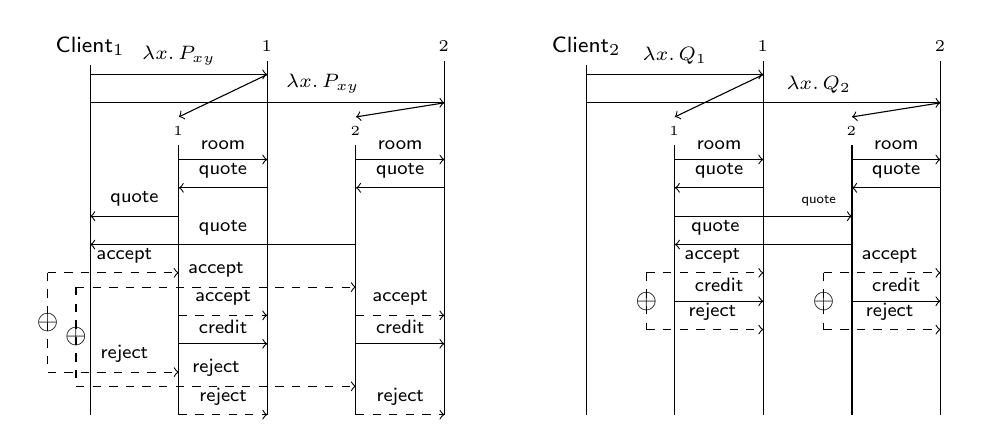
\begin{tikzpicture}[scale=0.9]
%	\draw[help lines]		(0, 0) grid (13, 10);

	%%%%%%%%%%%%%%%%%%%%% Scenario 1

	%%%% Nodes
	\node	(Client1)	at	(0, 10) {\footnotesize $\Client_1$};
	\node	(Hotel1)	at	(2.5, 10) {\footnotesize $\Hotel_1$};
	\node	(Hotel2)	at	(5, 10) {\footnotesize $\Hotel_2$};

	\node	(Code1)		at	(1.25, 8.8) {\scriptsize $\Code_1$};
	\node	(Code2)		at	(3.75, 8.8) {\scriptsize $\Code_2$};

	%%%% Lines for Nodes
%	\draw[dashed]		(Client1.south west) -- (Client1.south east);
	\draw
		let
			\p1 = (Client1.south),
			\p2 = (Hotel1.south),
			\p3 = (Hotel2.south),
			\p4 = (Code1.south),
			\p5 = (Code2.south)
		in
			(\x1, \y1) -- (\x1, 4.8)
			(\x2, \y2) -- (\x2, 4.8)
			(\x3, \y3) -- (\x3, 4.8)
			(\x4, \y4) -- (\x4, 4.8)
			(\x5, \y5) -- (\x5, 4.8);

	%%%% Arrows
	\draw[->]
		let
			\p1 = (Client1),
			\p2 = (Hotel1)
		in
			(\x1, 9.6) to node[above] {\scriptsize $\abs{x}{P_{xy}}$} (\x2, 9.6);

	\draw[->]
		let
			\p1 = (Client1),
			\p2 = (Hotel2)
		in
			(\x1, 9.2) to node[above] {\qquad \qquad \scriptsize $\abs{x}{P_{xy}}$} (\x2, 9.2);

	\draw[->]
		let
			\p1 = (Hotel1)
		in
			(\x1, 9.6) -- (Code1.north);

	\draw[->]
		let
			\p1 = (Hotel2)
		in
			(\x1, 9.2) -- (Code2.north);


	\draw[->]
		let
			\p1 = (Code1),
			\p2 = (Hotel1)
		in
			(\x1, 8.4) to node[above] {\scriptsize $\rtype$} (\x2, 8.4);

	\draw[->]
		let
			\p1 = (Code1),
			\p2 = (Hotel1)
		in
			(\x2, 8) to node[above] {\scriptsize $\Quote$} (\x1, 8);

	\draw[->]
		let
			\p1 = (Code2),
			\p2 = (Hotel2)
		in
			(\x1, 8.4) to node[above] {\scriptsize $\rtype$} (\x2, 8.4);
	\draw[->]
		let
			\p1 = (Code2),
			\p2 = (Hotel2)
		in
			(\x2, 8) to node[above] {\scriptsize $\Quote$} (\x1, 8);

	\draw[->]
		let
			\p1 = (Code1),
			\p2 = (Client1)
		in
			(\x1, 7.6) to node[above] {\scriptsize $\Quote$} (\x2, 7.6);

	\draw[->]
		let
			\p1 = (Code2),
			\p2 = (Client1)
		in
			(\x1, 7.2) to node[above] {\scriptsize $\Quote$} (\x2, 7.2);


	%%%% Choice 
	%% Client1 --> Code1
	\draw[dashed]
		let
			\p1 = (Client1),
			\p2 = (Code1)
		in
			(-0.6, 6.8) to node {$\oplus$} (-0.6, 5.4);
%			(\x1, 4.8) -- (\x2, 4.8)
%			(\x1, 2.8) -- (\x2, 2.8);

	\draw[dashed, ->]
		let
			\p1 = (Client1),
			\p2 = (Code1)
		in
			(-0.6, 6.8) to node[above] {\scriptsize ~~~$\accept$} (\x2, 6.8);

%	\draw[dashed]
%		let
%			\p1 = (Code1),
%			\p2 = (Hotel1)
%		in
%			(\x1, 6.4) -- (\x2, 6.4)
%			(\x1, 5.2) -- (\x2, 5.2)
%			(\x1, 4) -- (\x2, 4)
%			(\x1, 3.2) -- (\x2, 3.2);

	\draw[->,dashed]
		let
			\p1 = (Code1),
			\p2 = (Hotel1)
		in
			(\x1, 6.2) to node[above] {\scriptsize $\accept$} (\x2, 6.2);

	\draw[->]
		let
			\p1 = (Code1),
			\p2 = (Hotel1)
		in
			(\x1, 5.8) to node[above] {\scriptsize $\creditc$} (\x2, 5.8);

	\draw[dashed, ->]
		let
			\p1 = (Client1),
			\p2 = (Code1)
		in
			(-0.6, 5.4) to node[above] {\scriptsize ~~~$\reject$} (\x2, 5.4);

	\draw[dashed, ->]
		let
			\p1 = (Code1),
			\p2 = (Hotel1)
		in
			(\x1, 4.8) to node[above] {\scriptsize $\reject$} (\x2, 4.8);


	%%%% Choice 
	%% Client1 --> Code2
	\draw[dashed]
		let
			\p1 = (Client1),
			\p2 = (Code2)
		in
			(-0.2, 6.6) to node {$\oplus$} (-0.2, 5.2);
%			(\x1, 4.8) -- (\x2, 4.8)
%			(\x1, 2.8) -- (\x2, 2.8);

	\draw[dashed, ->]
		let
			\p1 = (Client1),
			\p2 = (Code2)
		in
			(-0.2, 6.6) to node[above] {\scriptsize $\accept$} (\x2, 6.6);

%	\draw[dashed]
%		let
%			\p1 = (Code1),
%			\p2 = (Hotel1)
%		in
%			(\x1, 6.4) -- (\x2, 6.4)
%			(\x1, 5.2) -- (\x2, 5.2)
%			(\x1, 4) -- (\x2, 4)
%			(\x1, 3.2) -- (\x2, 3.2);

	\draw[->,dashed]
		let
			\p1 = (Code2),
			\p2 = (Hotel2)
		in
			(\x1, 6.2) to node[above] {\scriptsize $\accept$} (\x2, 6.2);

	\draw[->]
		let
			\p1 = (Code2),
			\p2 = (Hotel2)
		in
			(\x1, 5.8) to node[above] {\scriptsize $\creditc$} (\x2, 5.8);

	\draw[dashed, ->]
		let
			\p1 = (Client1),
			\p2 = (Code2)
		in
			(-0.2, 5.2) to node[above] {\scriptsize $\reject$} (\x2, 5.2);

	\draw[dashed, ->]
		let
			\p1 = (Code2),
			\p2 = (Hotel2)
		in
			(\x1, 4.8) to node[above] {\scriptsize $\reject$} (\x2, 4.8);


	%%%%%%%%%%%%%%%%%%%%% Scenario 2

	%%%% Nodes
	\node	(Client1)	at	(7, 10) {\footnotesize $\Client_2$};
	\node	(Hotel1)	at	(9.5, 10) {\footnotesize $\Hotel_1$};
	\node	(Hotel2)	at	(12, 10) {\footnotesize $\Hotel_2$};

	\node	(Code1)		at	(8.25, 8.8) {\scriptsize $\Code_1$};
	\node	(Code2)		at	(10.75, 8.8) {\scriptsize $\Code_2$};


	\draw
		let
			\p1 = (Client1.south),
			\p2 = (Hotel1.south),
			\p3 = (Hotel2.south),
			\p4 = (Code1.south),
			\p5 = (Code2.south)
		in
			(\x1, \y1) -- (\x1, 4.8)
			(\x2, \y2) -- (\x2, 4.8)
			(\x3, \y3) -- (\x3, 4.8)
			(\x4, \y4) -- (\x4, 4.8)
			(\x5, \y5) -- (\x5, 4.8);

	%%%% Arrows
	\draw[->]
		let
			\p1 = (Client1),
			\p2 = (Hotel1)
		in
			(\x1, 9.6) to node[above] {\scriptsize $\abs{x}{Q_1}$} (\x2, 9.6);

	\draw[->]
		let
			\p1 = (Client1),
			\p2 = (Hotel2)
		in
			(\x1, 9.2) to node[above] {\qquad \qquad \scriptsize $\abs{x}{Q_2}$} (\x2, 9.2);

	\draw[->]
		let
			\p1 = (Hotel1)
		in
			(\x1, 9.6) -- (Code1.north);

	\draw[->]
		let
			\p1 = (Hotel2)
		in
			(\x1, 9.2) -- (Code2.north);


	\draw[->]
		let
			\p1 = (Code1),
			\p2 = (Hotel1)
		in
			(\x1, 8.4) to node[above] {\scriptsize $\rtype$} (\x2, 8.4);

	\draw[->]
		let
			\p1 = (Code1),
			\p2 = (Hotel1)
		in
			(\x2, 8) to node[above] {\scriptsize $\Quote$} (\x1, 8);

	\draw[->]
		let
			\p1 = (Code2),
			\p2 = (Hotel2)
		in
			(\x1, 8.4) to node[above] {\scriptsize $\rtype$} (\x2, 8.4);
	\draw[->]
		let
			\p1 = (Code2),
			\p2 = (Hotel2)
		in
			(\x2, 8) to node[above] {\scriptsize $\Quote$} (\x1, 8);

	\draw[->]
		let
			\p1 = (Code1),
			\p2 = (Code2)
		in
			(\x1, 7.6) to node[above] {\qquad \qquad \tiny $\Quote$} (\x2, 7.6);

	\draw[->]
		let
			\p1 = (Code2),
			\p2 = (Code1)
		in
			(\x1, 7.2) to node[above] {\scriptsize $\Quote$ \qquad \qquad \qquad} (\x2, 7.2);


	%%%% Choice
	% Client1 --> Hotel1
	\draw[dashed]
		let
			\p1 = (Code1),
			\p2 = (Hotel1)
		in
			(7.85, 6.8) to node {$\oplus$} (7.85, 6);
%			(\x1, 5.6) -- (\x2, 5.6)
%			(\x1, 4.8) -- (\x2, 4.8);

	\draw[dashed, ->]
		let
			\p1 = (Code1),
			\p2 = (Hotel1)
		in
			(7.85, 6.8) to node[above] {\scriptsize ~~$\accept$} (\x2, 6.8);

	\draw[->]
		let
			\p1 = (Code1),
			\p2 = (Hotel1)
		in
			(\x1, 6.4) to node[above] {\scriptsize $\creditc$} (\x2, 6.4);

	\draw[dashed, ->]
		let
			\p1 = (Code1),
			\p2 = (Hotel1)
		in
			(7.85, 6) to node[above] {\scriptsize ~~$\reject$} (\x2, 6);

	% Client2 --> Hotel2
	\draw[dashed]
		let
			\p1 = (Code2),
			\p2 = (Hotel2)
		in
			(10.35, 6.8) to node {$\oplus$} (10.35, 6);
%			(\x1, 5.6) -- (\x2, 5.6)
%			(\x1, 4.8) -- (\x2, 4.8);

	\draw[dashed, ->]
		let
			\p1 = (Code2),
			\p2 = (Hotel2)
		in
			(10.35, 6.8) to node[above] {\scriptsize ~~$\accept$} (\x2, 6.8);

	\draw[->]
		let
			\p1 = (Code2),
			\p2 = (Hotel2)
		in
			(\x1, 6.4) to node[above] {\scriptsize $\creditc$} (\x2, 6.4);

	\draw[dashed, ->]
		let
			\p1 = (Code2),
			\p2 = (Hotel2)
		in
			(10.35, 6) to node[above] {\scriptsize ~~$\reject$} (\x2, 6);

\end{tikzpicture}
%\end{center}

\caption{Sequence diagrams for $\Client_1$ and $\Client_2$\label{fig:exam}.}
\end{figure}

 
The different protocols implemented by $\Client_1$ and $\Client_2$ can be represented by the sequence diagrams of \figref{fig:exam}. 


\begin{example}[The Hotel Booking Example, Revisited]\label{exam:type}
We give types to the client
processes. % of~\secref{exam:proc}.
Assume 
\begin{eqnarray*}
S & = & \btout{\Quote} \btbra{\accept: \tinact, \reject: \tinact} \\
U & = & \btout{\rtype} \btinp{\Quote} \btsel{\accept: \btout{\creditc} \tinact, \reject: \tinact }
\end{eqnarray*}
While the typing for $\abs{x}{P_{xy}}$ is $\es; \es; y: S \proves \abs{x}{P_{xy}} \hastype \lhot{U}$,
the typing for $\Client_1$ is
$~~
	\es; \es; s_1: \btout{\lhot{U}} \tinact \cat s_2: \btout{\lhot{U}} \tinact \proves \Client_1 \hastype \Proc
$.


The typings for $Q_1$ and $Q_2$ are
$	\es; \es; y: \btout{\Quote} \btinp{\Quote} \tinact \proves \abs{x}{Q_i} \hastype \lhot{U}
$ ($i=1,2$)
and the type for $\Client_2$ is
$~~
	\es; \es; s_1: \btout{\lhot{U}} \tinact \cat s_2: \btout{\lhot{U}} \tinact \proves \Client_2 \hastype \Proc
$.
\end{example}


\begin{proposition}\label{p:examp}
	Let
	$S = \btout{\rtype} \btinp{\Quote} \btsel{\accept: \btout{\creditc} \tinact, \reject: \tinact}$
	and
	$\Delta = s_1: \btout{\lhot{S}} \tinact \cat s_2: \btout{\lhot{S}} \tinact$.
%	\begin{eqnarray*}
%		S &=& \btout{\rtype} \btinp{\Quote} \btsel{\accept: \btout{\creditc} \tinact, \reject: \tinact}\\
%		\Delta &=& s_1: \btout{\lhot{S}} \tinact \cat s_2: \btout{\lhot{S}} \tinact
%	\end{eqnarray*}
	Then
	$\horel{\es}{\Delta}{\Client_1}
	{\fwb}
	{\Delta}{\Client_2}$, where $\Client_1$ and $\Client_2$ are as above.
	%in \secref{exam:proc}. 
\end{proposition}

\section{Correctness Criteria for Typed Encodings}
\label{s:expr}
%% !TEX root = main.tex

%%%%
% COMMANDS
% Parameters - 1:Gamma , 2:label, 3:initial delta, 4:initial processes, 5:final delta, 6:final process

%\newcommand{\stytra}[6]{\ensuremath{#1; \emptyset; #3 \hby{#2} #5 \proves #4  \hby{#2} #6 }}
\newcommand{\stytra}[6]{\ensuremath{#1; #3 \proves #4 \hby{#2} #1; #5 \proves #6 }}

%\newcommand{\wtytra}[6]{\ensuremath{#1; \emptyset; #3 \Hby{#2} #5 \proves #4  \Hby{#2} #6 }}
\newcommand{\wtytra}[6]{\ensuremath{#1; #3 \proves #4 \Hby{#2} #1; #5 \proves #6 }}

%\newcommand{\wbb}[6]{\ensuremath{#1; \emptyset; #3 \wb #5 \proves #4  \wb #6 }}
\newcommand{\wbb}[6]{\ensuremath{#1; #3 \proves #4 \wb #1; #5 \proves #6 }}

%%%%%%%%%%


\newpage
\section{Typed Encodings}\label{s:expr}

We define the notion of \emph{typed encoding} that we
shall use in the following section.
%In general, we may define:

\begin{definition}[Typed Calculus]\label{d:tcalculus}\rm
	A \emph{typed calculus} $\tyl{L}$ is a tuple
$		\calc{L}{T}{\hby{\ell}}{\wb}{\proves}$
	where $L$ and $T$ are set of processes and types, respectively.
	Also, $\hby{\ell}$, $\wb$, and $\proves$ 
	denote a transition semantics, a typed process equivalence, and a type system for $L$ processes, respectively. 
\end{definition}

Since we study subcalculi of $\HOp$, 
the typed calculi considered here 
use the same 
  type system (as in \S\,\ref{s:types}),
 transition semantics (cf. Def.~\ref{d:tlts}) with labels $\ell$ (as in  \S\,\ref{ss:lts}), 
 and behavioral equivalence (cf. Def.~\ref{d:bisim}). 
  Thus, in the following, when writing $\tyl{L}_i$ we tacitly assume the existence of appropriate 
  $L_i$ and $T_i$, keeping all other elements unchanged.
 We now define the notion of encoding over typed calculi.

\begin{definition}[Typed Encoding]\rm
	Let  $\tyl{L}_1$ % = \calc{L_1}{T_1}{\red_1}{\wb_1}{\proves_1}$
	and $\tyl{L}_2$ % =  \calc{L_2}{T_2}{\red_2}{\wb_2}{\proves_2}$ 
	be typed calculi. % as in Definition~\ref{d:tcalculus}.
	Given mappings $\map{\cdot}: L_1 \to L_2$, 
	$\mapt{\cdot}: T_1 \to T_2$, and 
	$\mapa{\cdot}: \ell \to \ell^{\,m}$, 
	we write 
	%$\enc{\cdot}{\cdot}: \calc{L_1}{T_1}{\red_1}{\wb_1}{\proves_1} \longrightarrow \calc{L_2}{T_2}{\red_2}{\wb_2}{\proves_2}$
%	for the encoding from $\calc{L_1}{T_1}{\red_1}{\wb_1}{\proves_1}$ to $\calc{L_2}{T_2}{\red_2}{\wb_2}{\proves_2}$.
	$\enco{\map{\cdot}, \mapt{\cdot}, \mapa{\cdot}} : \tyl{L}_1 \to \tyl{L}_2$
	to denote the \emph{typed encoding} of $\tyl{L}_1$ into $\tyl{L}_2$.
\end{definition}

Our notion of encoding considers a mapping on processes, 
% mapping $\map{\cdot}$,
a mapping on types, % $\mapt{\cdot}$, 
and a mapping %$\mapa{\cdot}$ 
from transition labels 
into \emph{sets} of transition labels.
We will often assume that  $\mapt{\cdot}$ extends to typing environments as expected.
As we will define several typed encodings,  
in the following we use number decorations on these mappings, to distinguish them.






%\subsection{Encoding Properties}
%We use the following labeled transitions:
%\begin{enumerate}
%\item Strong case: $\Gamma; \emptyset; \Delta_1 \hby{\ell} \Delta_1' \proves P_1 \hby{\ell} P_2$ \\
%(With the new command: $\stytra{\Gamma}{\ell}{\Delta_1}{P_1}{\Delta'_1}{P_2}$)
%\item Weak case: $\Gamma; \emptyset; \Delta_1 \Hby{ \ell} \Delta_1' \proves P_1 \Hby{ \ell} P_2$ \\
%(With the new command: $\wtytra{\Gamma}{\ell}{\Delta_1}{P_1}{\Delta'_1}{P_2}$)
%\item Using the command for weak bisimilarity:
%$\wbb{\Gamma}{\ell}{\Delta_1}{P_1}{\Delta'_1}{P_2}$.
%
%\end{enumerate}

We require that a {\em good} typed encoding should 
preserve not only the syntax but
also the operational, typing and behavioural
semantics. 

% ----> DK: The next notation is already defined
%\begin{notation}[Typed Equivalence]\rm
%	Let $P$ and $Q$ be two well-typed processes, i.e., 
%	there exist $\Gamma, \Sigma_1, \Sigma_2$ such that 
%	$\Gamma; \emptyset; \Sigma_1 \proves P \hastype \Proc$ 
%	and
%	$\Gamma; \emptyset; \Sigma_2 \proves Q \hastype \Proc$.
%	Then, to denote the fact that 
%	$P$ and $Q$ are related by behavioral equivalence $\wb$, we shall write
%	%Then we adopt the following notational convention:
%	\[
%		\Gamma; \Sigma_1 \wb \Sigma_2 \proves P \wb Q.
%	\]
%\end{notation}

\begin{definition}[Semantic Preserving Encoding]\rm
	\label{def:ep}
	We say that $\enco{\map{\cdot}, \mapt{\cdot}, \mapa{\cdot}}: \tyl{L}_1 \to \tyl{L}_2$ is a \emph{semantic preserving encoding}
	if it satisfies the following properties:
	
	\begin{enumerate}[1.]
		\item \emph{Type preservation}:
		if
			$\Gamma; \emptyset; \Delta \proves P \hastype \Proc$ then 
			$\mapt{\Gamma}; \emptyset; \mapt{\Delta} \proves \map{P} \hastype \Proc$,  
			for any   $P$ in $L_1$.

		\item \emph{Operational Correspondence}: If $\Gamma; \emptyset; \Delta \proves P \hastype \Proc$ then
		\begin{enumerate}[-]
%			\item	Completeness: \\
%			    If $P \red_1 P'$ then $\exists\, \Delta'$ s.t.
%				$\map{P} \Red_2 \map{P'}$ and
%				$\mapt{\Gamma}; \emptyset; \mapt{\Delta'} \proves_2 \map{P'} \hastype \Proc$.
			\item	Completeness: 
			   If  $\stytra{\Gamma}{\ell_1}{\Delta_1}{P}{\Delta'_1}{P'}$
			   then \\ $\exists \ell_2$ s.t. 
			    $\wtytra{\mapt{\Gamma}}{\ell_2}{\mapt{\Delta_1}}{\map{P}}{\mapt{\Delta'_1}}{\map{P'}}$
			    and $\ell_2 = \mapa{\ell_1}$.
			    				
%			\item Soundness : \\
%			    If $\map{P} \red_2 Q$ then
%				$\exists P'$ s.t. $P \red_1 P'$ and 
%				$\mapt{\Gamma}; \mapt{\Delta_1} \wb_2 \mapt{\Delta_2} \proves_2 \map{P'} \wb_2 Q$.
				
			\item Soundness:   
			If  $\wtytra{\mapt{\Gamma}}{\ell_2}{\mapt{\Delta_1}}{\map{P}}{\mapt{\Delta'_1}}{Q}$
			   then $\exists \ell_1, P'$ s.t.  \\
			    (i)~$\stytra{\Gamma}{\ell_1}{\Delta_1}{P}{\Delta'_1}{P'}$,
			    (ii)~$\ell_2 = \mapa{\ell_1}$, and
			    (iii)~$\wbb{\mapt{\Gamma}}{\ell}{\mapt{\Delta'_1}}{\map{P'}}{\mapt{\Delta'_1}}{Q}$.
		\end{enumerate}
		
		\item \emph{Full Abstraction:} \\
%		$\Gamma; \Delta_1 \wb \Delta_2 \proves P \wb Q $ if and only if $\mapt{\Gamma}; \mapt{\Delta_1} \wb \mapt{\Delta_2} \proves \map{P} \wb \map{Q} $.
		\wbb{\Gamma}{}{\Delta_1}{P}{\Delta_2}{Q}
		if and only if
		\wbb{\mapt{\Gamma}}{}{\mapt{\Delta_1}}{\map{P}}{\mapt{\Delta_2}}{\map{Q}}.
	\end{enumerate}
\end{definition}

\begin{remark}\label{r:multilabels}
We  assume that if 
$P \hby{\ell} P'$ and $\mapa{\ell} = \{\ell_1, \ell_2,  \cdots, \ell_m\}$ then
$\map{P} \Hby{\mapa{\ell}} \map{P'}$
should be understood as
$\map{P} \Hby{\ell_1} P_1 \Hby{\ell_2} P_2 \cdots \Hby{\ell_m} P_m =  \map{P'}$,
for some
$P_1, P_2, \ldots, P_m$.
This is useful for the encoding of polyadic into monadic communication.
\end{remark}

We show that the composition of encodings is closed on the above properties.

\begin{proposition}[Composability of Semantic Preserving Encodings]
	Let 
	$\enco{\map{\cdot}^{1}, \mapt{\cdot}^{1}, \mapa{\cdot}^{1}}: \tyl{L}_1 \to \tyl{L}_2$
	and 
	$\enco{\map{\cdot}^{2}, \mapt{\cdot}^{2}, \mapa{\cdot}^{2}}: \tyl{L}_2 \to \tyl{L}_3$
%	$\enco{\cdot}{\cdot}{1}: \tyl{L}_1 \to \tyl{L}_2$ and $\encod{\cdot}{\cdot}{2}: \tyl{L}_2 \to \tyl{L}_3$
	be two semantic preserving encodings.
	Then their composition, denoted 
	$\enco{\map{\cdot}^{1} \circ \map{\cdot}^{2}, \mapt{\cdot}^{1} \circ \mapt{\cdot}^{2}, \mapa{\cdot}^{1}\circ \mapa{\cdot}^{2}}: \tyl{L}_1 \to \tyl{L}_3$
	is also a semantic preserving encoding.
\end{proposition}

\begin{proof}
	Straightforward application of the definition of each property.
\end{proof}

\section{Positive Expressiveness Results}
In this section we present a study of the expressiveness of $\HOp$ and its subcalculi. 


\begin{comment}
\subsection{Languages Under Consideration}
We consider the following variants of \HOp:
\begin{enumerate}[-]
	\item	\HO: the second and third lines of the syntax of processes in Fig.~\ref{fig:syntax} (pure higher-order, monadic communication).
	\item	\sesp: the first and third lines of the syntax of processes in Fig.~\ref{fig:syntax} (first-order, monadic communication).
	\item	\sespnr: the finite sub-calculus of \sesp, i.e., name passing without recursion.
	\item	$\HO^{+\mathsf{p}}$: The polyadic \HO, i.~e.\ without polyadicity (polyadic abstraction/application).
	\item	$\sesp^{+\mathsf{p}}$: The polyadic \sesp, i.~e.\ with polyadicity (name passing)
	\item	$\HOp^{-\mathsf{p}}$: The monadic \HOp.
%	\item \pHOpnr: the finite variant of \pHOp 
%	\item \psesp: the variant of \sesp with polyadic communication.
%	\item \psespnr: the finite variant of \psesp with polyadic communication.
\end{enumerate}
\noindent
In the following we write $\pmap{\cdot}{i}$
and $\tmap{\cdot}{i}$ 
for mappings of processes and types, respectively.
Since we always consider variants and fragments of \HOp, the 
reduction semantics $\red$, the typed behavioral equivalence $\wb$,
and the type system $\proves$ are the same for all languages.
\end{comment}

\subsection{Encoding Polyadic Semantics (\HOp) to Monadic Semantics ($\HOp^{-\mathsf{p}}$)}\label{ss:polmon}

%In the extension of \HOp with 
%polyadic communication, denoted \pHOp, 
%one may pass in each synchronization 
%a tuple of values of length $n$, rather than a just single value.
%Thus, e.g., for $n = 2$ one would have
%%
%\begin{eqnarray*}
%	\bout{n}{m_1, m_2} P \Par \binp{\dual{n}}{x_1,x_2} Q  & \red &  P \Par Q \subst{m_1, m_2}{x_1, x_2} \\
%	\bout{n}{\abs{x_1, x_2}{P_1}} P \Par \binp{\dual{s}}{\X} Q & \red & P \Par Q \subst{\abs{x_1,x_2}{P_1}}{\X}
%\end{eqnarray*}
%%
%with $\appl{X}{k_1,k_2} \subst{\abs{x_1,x_2}{Q}}{\X}  =  Q \subst{k_1,k_2}{x_1,x_2} $.
%Thus, 
%\pHOp features tuple passing in intra-session (linear) communication,
%but also in abstractions/applications. 
%The session type system for \pHOp is an orthogonal
%extension of that in \S\,\ref{s:types}.
%The type syntax for values is extended as follows,
%where $\tilde{S}$ stands for a sequence $S_1, \ldots, S_n$ of 
%session types:
%
%\begin{eqnarray*}
%	U \bnfis  & \tilde{S} \bnfbar \lhot{\tilde{S}} \bnfbar \shot{\tilde{S}} \bnfbar \chtype{S}
%\end{eqnarray*}
%
%The syntax of session types would be kept unchanged.
%Typing rules require straightforward extensions. 
%For instance, the following rules would type 
%abstraction and application in the biadic case ($n = 2$):
%\[
%\trule{Abs2}~~\tree{
%			\Gamma; \Lambda; \Sigma \cat x_1: S_1, x_2: S_2 \proves P \hastype \Proc
%		}{
%			\Gamma; \Lambda; \Sigma \proves \abs{x_1, x_2}{P} \hastype \lhot{(S_1, S_2)}
%		}
%		\quad
%		\trule{App2}~~\tree{
%		\begin{array}{c}
%		(U = \lhot{(S_1,S_2)}) \lor (U = \shot{(S_1,S_2)}) \\
%		\Gamma; \Lambda; \Sigma \proves X \hastype U  \\
%		\Gamma; \Lambda_1; \Sigma_1 \proves k_1 \hastype S_1 \quad 		
%		\Gamma; \Lambda_2; \Sigma_2 \proves k_2 \hastype S_2
%		\end{array}
%		}{
%			\Gamma; \Lambda \cup  \Lambda_1 \cup \Lambda_2; \Sigma \cup \Sigma_1 \cup \Sigma_2 \proves \appl{X}{k_1,k_2} \hastype \Proc
%		} 
%\]

In the untyped $\pi$-calculus, polyadic communication
can be encoded into monadic name passing by first generating a fresh channel and then 
performing $n$ monadic synchronizations on that channel. 
In session-typed $\pi$-calculi this encoding is even more direct, 
thanks to the linearity and non-interference  of session endpoints~\cite{VascoFun}.
%The extension of the (monadic) session type system given in \S\,\ref{s:types}
%to handle polyadic communication is straightforward and follow expected lines.
%For this reason, we do not present a typing system for \pHOp in full detail; rather, 
%we shall define a syntactic transformation of \pHOp into \HOp, rather than as a typed encoding.
%\footnote{The definition of a polyadic semantics would only add visual clutter to our presentation,
%as all results extend easily from monadic to polyadic communication.}
Below we  define an encoding of polyadic semantics to monadic semantics.
Using this encoding, %Because of the polyadic to monadic encoding %, denoted  $\auxmap{\cdot}{\mathsf{p}}$,
we may focus on monadic session processes,
and rely on polyadic constructs simply as convenient syntactic sugar.
In fact, we shall rely on polyadicity to encode recursive behaviors.
%
\begin{definition}[Polyadic Into Monadic]\label{d:enc:poltomon}
Let 
$\enco{\map{\cdot}^{\mathsf{p}}, \mapt{\cdot}^{\mathsf{p}}, \mapa{\cdot}^{\mathsf{p}}}: \HOp \to \HOp^{-\mathsf{p}}$
be a typed encoding where
	%$\auxmap{\cdot}{\mathsf{p}}:\pHOp \to \HOp$ as
\begin{figure}[t]
\[
	\begin{array}{rcl}
		\map{\bout{k}{k_1, \cdots, k_m} P}^{\mathsf{p}}
		&\defeq&
		\bout{k}{k_1} \cdots ;  \bout{k}{k_m} \map{P}^{\mathsf{p}}
		\\
			\map{\binp{k}{x_1, \cdots, x_m} P}^{\mathsf{p}}
		&\defeq&
		\binp{k}{x_1} \cdots ; \binp{k}{x_m}  \map{P}^{\mathsf{p}}
		\\
		\map{\bbout{k}{\abs{x_1, \cdots, x_m} Q} P}^{\mathsf{p}}
		&\defeq&
		\bbout{k}{\abs{z}\binp{z}{x_1} \cdots ; \binp{z}{x_m} \map{Q}^{\mathsf{p}}} \map{P}^{\mathsf{p}}
		\\ 
		\map{\appl{X}{k_1, \cdots, k_m}}^{\mathsf{p}}
		&\defeq&
		\newsp{s}{\appl{X}{s} \Par \bout{\dual{s}}{k_1} \cdots ; \bout{\dual{s}}{k_m} \inact} 
        \\ % typed mapping starts here
		\tmap{\btout{S_1, \cdots, S_m}S}{\mathsf{p}}
		&\defeq&
		\btout{\tmap{S_1}{\mathsf{p}}} \cdots ; \btout{\tmap{S_m}{\mathsf{p}}}\tmap{S}{\mathsf{p}}
		\\
		\tmap{\btinp{S_1, \cdots, S_m}S}{\mathsf{p}}
		&\defeq&
		\btinp{\tmap{S_1}{\mathsf{p}}} \cdots ; \btinp{\tmap{S_m}{\mathsf{p}}}\tmap{S}{\mathsf{p}}
		\\
		\tmap{\bbtout{\lhot{(C_1, \cdots, C_m)}} S}{\mathsf{p}}
		&\defeq&
		\bbtout{
		\lhot{\big(\btinp{\tmap{C_1}{\mathsf{p}}} \cdots ;\btinp{\tmap{C_m}{\mathsf{p}}}\tinact\big)}}\mapt{S}^{\mathsf{p}}
		\\
		\tmap{\bbtinp{\lhot{(C_1, \cdots, C_m)}} S}{\mathsf{p}}
		&\defeq&
		\bbtinp{
		\lhot{\big(\btinp{\tmap{C_1}{\mathsf{p}}} \cdots; \btinp{\tmap{C_m}{\mathsf{p}}}\tinact\big)}}\mapt{S}^{\mathsf{p}}
		\\
		\tmap{\bbtout{\shot{(C_1, \cdots, C_m)}} S}{\mathsf{p}}
		&\defeq&
		\bbtout{
		\shot{\big(\btinp{\tmap{C_1}{\mathsf{p}}} \cdots; \btinp{\tmap{C_m}{\mathsf{p}}}\tinact\big)}}\mapt{S}^{\mathsf{p}}
		\\
		\tmap{\bbtinp{\shot{(C_1, \cdots, C_m)}} S}{\mathsf{p}}
		&\defeq&
		\bbtinp{
		\shot{\big(\btinp{\tmap{C_1}{\mathsf{p}}} \cdots; \btinp{\tmap{C_m}{\mathsf{p}}}\tinact\big)}}\mapt{S}^{\mathsf{p}}
%		\\
%		\tmap{\lhot{(C_1, \cdots, C_m)}}{\mathsf{p}}
%		&\defeq&
%		\lhot{\big(\btinp{\tmap{C_1}{\mathsf{p}}} \cdots \btinp{\tmap{C_m}{\mathsf{p}}}\tinact\big)}
%		\\
%		\tmap{\shot{(C_1, \cdots, C_m)}}{\mathsf{p}}
%		&\defeq&
%		\shot{\big(\btinp{\tmap{C_1}{\mathsf{p}}} \cdots \btinp{\tmap{C_m}{\mathsf{p}}}\tinact\big)}
		\\ % action mapping starts here
		\mapa{\bactout{k}{k_1, \ldots, k_m}}^\mathsf{p} &\defeq&   \big\{\bactout{k}{k_1}, \cdots, \bactout{k}{k_m}\big\} \\
		\mapa{\bactinp{k}{k_1, \ldots, k_m}}^\mathsf{p} &\defeq&   \big\{\bactinp{k}{k_1}, \cdots, \bactinp{k}{k_m} \big\}\\
		\mapa{\bactout{k}{\abs{x_1, \ldots, x_m}{P}} }^\mathsf{p} &\defeq&  \bactout{k}{\abs{z}\binp{z}{x_1} \cdots ; \binp{z}{x_m} \map{P}^{\mathsf{p}}} \\
		\mapa{\bactinp{k}{\abs{x_1, \ldots, x_m}{P}} }^\mathsf{p} &\defeq&  \bactinp{k}{\abs{z}\binp{z}{x_1} \cdots ; \binp{z}{x_m} \map{P}^{\mathsf{p}}} 
	\end{array}
\]
\caption{
Encoding of polyadic into monadic communication (cf.~Defintion \ref{d:enc:poltomon} \label{f:enc:poltomon}).
The mappings are homomorphisms for the other processes/types/labels. 
}
\end{figure}
mappings $\map{\cdot}^{\mathsf{p}}$, $\mapt{\cdot}^{\mathsf{p}}$, $\mapa{\cdot}^{\mathsf{p}}$
are 
as in Fig.~\ref{f:enc:poltomon}.
	%\jp{I prefer to be explicit in the encoding of polyadic abstraction/applications. Previous version is commented.}
\end{definition}
%
The encoding is simple:
passing an $m$-tuple of names over a session channel $k$ is represented by 
a $m$ exchanges along channel $k$.
The output of an abstraction with $m$ bound variables $x_1, \ldots, x_m$ is represented by
outputting an abstraction with a single bound variable $z$,
which is used as the subject for receiving $x_1, \ldots, x_m$ individually. 
Accordingly, 
%When we are dealing with an abstraction over a list of bound variables,
%then we create a new abstraction name and we use it to receive in a polyadic
%way the list of names on the abstraction. Similarly 
the encoding of a polyadic application  instantiates
the abstraction subject with a freshly generated session name $s$, which will be used  
to the names 
$k_1, \ldots, k_m$
that are going to be applied on the abstraction.
Observe how $\mapa{\cdot}$ maps polyadic labels for input and output into (ordered) sets of
monadic labels. Also, note that we do not allow polyadic mapping on shared names.
The polyadic mapping, as presented here, is sound only on session names.
%The semantics might break if we apply this mapping on shared names.

%\begin{proposition}
%	$\Gamma; \emptyset; \Sigma \proves \map{P}^{p} \hastype \Proc$
%\end{proposition}

\begin{proposition}[Type Preservation, Polyadic to Monadic]
Let $P$ be an  $\HOp$ process.
If			$\Gamma; \emptyset; \Delta \proves P \hastype \Proc$ then 
			$\mapt{\Gamma}^{\mathsf{p}}; \emptyset; \mapt{\Delta}^{\mathsf{p}} \proves \map{P}^{\mathsf{p}} \hastype \Proc$. 
\end{proposition}

\begin{proof}
By induction on the inference $\Gamma; \emptyset; \Delta \proves P \hastype \Proc$.
	\qed
\end{proof}

\begin{proposition}\label{p:poltomo}
If $\map{P\subst{\abs{x_1, \cdots, x_m} Q}{X}}^{\mathsf{p}} = \map{P}^{\mathsf{p}}\subst{\abs{z}\binp{z}{x_1} \cdots ; \binp{z}{x_m} \map{Q}^{\mathsf{p}}}{X}$.
\end{proposition}
\begin{proof}
Immediate from the definition of $\map{\cdot}^{\mathsf{p}}$ (cf. Def.~\ref{d:enc:poltomon}).
	\qed
\end{proof}


\begin{proposition}[Operational Correspondence, Polyadic to Monadic]
Let $P$ be an  $\HOp$ process.
If $\Gamma; \emptyset; \Delta \proves P \hastype \Proc$ then
		\begin{enumerate}[a)]
			\item	 
			   If  $\stytra{\Gamma}{\ell_1}{\Delta}{P}{\Delta'}{P'}$
			   then  $\exists \ell_2$ s.t. 
			    $\wtytra{\mapt{\Gamma}^{\mathsf{p}}}{\ell_2}{\mapt{\Delta}^{\mathsf{p}}}{\map{P}}{\mapt{\Delta'}^{\mathsf{p}}}{\map{P'}}$
			    and $\ell_2 = \mapa{\ell_1}^{\mathsf{p}}$.
			    
			\item   
			If  $\wtytra{\mapt{\Gamma}^{\mathsf{p}}}{\ell_2}{\mapt{\Delta_1}^{\mathsf{p}}}{\map{P}}{\mapt{\Delta'_1}^{\mathsf{p}}}{Q}$
			   then $\exists \ell_1, P$ s.t.  
			    (i)~$\stytra{\Gamma}{\ell_1}{\Delta_1}{P}{\Delta'_1}{P'}$, \\
			    (ii)~$\ell_2 = \mapa{\ell_1}^{\mathsf{p}}$, 
			    (iii)~$\wbb{\mapt{\Gamma}^{\mathsf{p}}}{\ell}{\mapt{\Delta'_1}^{\mathsf{p}}}{\map{P'}^{\mathsf{p}}}{\mapt{\Delta'_1}^{\mathsf{p}}}{Q}$.
			    \end{enumerate}
\end{proposition}

\begin{proof}
By transition induction.
%, considering Remark~\ref{r:multilabels} for weak transitions. All cases are easy;
%we only remark that the additional $\tau$-transitions induced by the encoding 
%are directly associated to the polyadicity involved. This is particularly relevant
%when $\ell_1 = \bactinp{n}{\abs{\tilde{x}}{P}}$, for the encoding of a polyadic application involves
%as many $\tau$-transitions (i.e., synchronizations on the restricted name $s$) 
%as polyadic parameters are involved.	\\
We consider parts (a) and (b) separately: \\
\noi \textbf{Part (a)}. We consider two non-trivial cases, using biadic communication:
\begin{enumerate}[1.]

%% Biadic Output 
\item Case  $P =\bout{k}{k_1, k_2} P'$ and $\ell_1 = \bactout{k}{k_1, k_2}$. By assumption, $P$ is well-typed. 
We may have:
			\[
				\tree{
					\Gamma; \emptyset; \Delta_0 \cat k:S  \proves  P' \hastype \Proc \quad 
					\Gamma ; \emptyset ; k_1{:} S_1 \cat k_2{:}S_2 \proves  k_1,k_2 \hastype S_1,S_2}{
					\Gamma; \emptyset; \Delta_0 \cat k_1{:}S_1 \cat k_2{:}S_2 \cat k:\btout{S_1,S_2}S \proves  
					\bout{k}{k_1,k_2} P' \hastype \Proc}
			\]
for some $\Gamma, S, S_1, S_2, \Delta_0$, 
such that $\Delta = \Delta_0 \cat k_1{:}S_1 \cat k_2{:}S_2 \cat k:\btout{S_1,S_2}S$.
We may then have the following typed transition
$$
\stytra{\Gamma}{\ell_1}{\Delta_0 \cat k_1{:}S_1 \cat k_2{:}S_2 \cat k:\btout{S_1,S_2}S}{\bout{k}{k_1, k_2} P'}{\Delta_0 \cat k{:}S}{P'}
$$
The encoding of the source judgment for $P$ is as follows:
$$
\mapt{\Gamma}^{\mathsf{p}}; \emptyset; \mapt{\Delta_0 \cat k_1{:}S_1 \cat k_2{:}S_2 \cat k:\btout{S_1,S_2}S}^{\mathsf{p}} \proves \map{\bout{k}{k_1, k_2} P'}^{\mathsf{p}} \hastype \Proc
$$
which, using Def.~\ref{d:enc:poltomon}, can be equivalently expressed as 
$$
\mapt{\Gamma}^{\mathsf{p}}; \emptyset; \mapt{\Delta_0} 
\cat k_1{:}\mapt{S_1}^{\mathsf{p}} \cat k_2{:}\mapt{S_2}^{\mathsf{p}} 
\cat k:\btout{\mapt{S_1}^{\mathsf{p}}}\btout{\mapt{S_2}^{\mathsf{p}}}\mapt{S}^{\mathsf{p}}
\proves 
\bout{k}{k_1}\bout{k}{k_2} \map{P'}^{\mathsf{p}} 
\hastype \Proc
$$
Now, $\mapa{\ell_1}^{\mathsf{p}} = \{ \bactout{k}{k_1 }, \bactout{k}{ k_2}\}$. 
It is immediate to infer the following typed transitions for $\map{P}^{\mathsf{p}}  = \bout{k}{k_1}\bout{k}{k_2} \map{P'}^{\mathsf{p}} $:
\begin{eqnarray*}
& & \mapt{\Gamma}^{\mathsf{p}}; 
\mapt{\Delta_0} \cat  k_1{:}\mapt{S_1}^{\mathsf{p}} \cat k_2{:}\mapt{S_2}^{\mathsf{p}} \cat
k:\btout{\mapt{S_1}^{\mathsf{p}}}\btout{\mapt{S_2}^{\mathsf{p}}}\mapt{S}^{\mathsf{p}}
\proves 
\bout{k}{k_1}\bout{k}{k_2} \map{P'}^{\mathsf{p}}  \\
& \hby{\bactout{k}{k_1}} & 
\mapt{\Gamma}^{\mathsf{p}}; \mapt{\Delta_0} \cat  k_1{:}\mapt{S_1}^{\mathsf{p}} \cat k_2{:}\mapt{S_2}^{\mathsf{p}} \cat
k:\btout{\mapt{S_2}^{\mathsf{p}}}\mapt{S}^{\mathsf{p}}
\proves 
\bout{k}{k_2} \map{P'}^{\mathsf{p}} \\
& \hby{\bactout{k}{k_2}} & 
\mapt{\Gamma}^{\mathsf{p}}; \mapt{\Delta_0} \cat  k_1{:}\mapt{S_1}^{\mathsf{p}} \cat k_2{:}\mapt{S_2}^{\mathsf{p}} \cat
\mapt{S}^{\mathsf{p}}
\proves 
 \map{P'}^{\mathsf{p}} \\
 & = & 
 \mapt{\Gamma}^{\mathsf{p}}; \mapt{\Delta_0 \cat
k:S \cat
k_1{:}S_1 \cat
k_2{:}S_2}^{\mathsf{p}}
\proves 
 \map{P'}^{\mathsf{p}}
\end{eqnarray*}
which concludes the proof for this case.

%% Biadic Abstraction Output 
\item Case  $P = \bbout{k}{\abs{x_1, x_2} Q} P' $ and $\ell_1 = \bactout{k}{\abs{x_1, x_2}{Q}}$. 
By assumption, $P$ is well-typed. 
We may have:
			\[
				\tree{
					\Gamma; \emptyset; \Delta_0 \cat k:S  \proves  P' \hastype \Proc \quad 
					\Gamma ; \emptyset ; \Delta_1 \proves  \abs{x_1,x_2}Q \hastype \lhot{(C_1,C_2)}}{
					\Gamma; \emptyset; \Delta_0 \cat \Delta_1 \cat k:\btout{\lhot{(C_1,C_2)}}S \proves  
					\bout{k}{\abs{x_1,x_2}Q} P' \hastype \Proc}
			\]
for some $\Gamma, S, C_1, C_2, \Delta_0, \Delta_1$, 
such that $\Delta = \Delta_0 \cat \Delta_1 \cat  k:\btout{\lhot{(C_1,C_2)}}S$.
(For simplicity, we consider only the case of a linear function.)
We may have the following typed transition:
$$
\stytra{\Gamma}{\ell_1}{\Delta_0 \cat \Delta_1 \cat k:\bbtout{\lhot{(C_1, C_2)}}S}{\bbout{k}{\abs{x_1, x_2} Q} P' }{\Delta_0 \cat k{:}S}{P'}
$$
The encoding of the source judgment is
$$
\mapt{\Gamma}^{\mathsf{p}}; \emptyset; \mapt{\Delta_0 \cat \Delta_1 \cat k:\bbtout{\lhot{(C_1, C_2)}}S}^{\mathsf{p}} \proves \map{\bbout{k}{\abs{x_1, x_2} Q} P' }^{\mathsf{p}} \hastype \Proc
$$
which, using Def.~\ref{d:enc:poltomon}, can be equivalently expressed as 
$$
\mapt{\Gamma}^{\mathsf{p}}; \emptyset; \mapt{\Delta_0 \cat \Delta_1} \cat
%k:\btout{\mapt{S_1}^{\mathsf{p}}}\btout{\mapt{S_2}^{\mathsf{p}}}\mapt{S}^{\mathsf{p}}
k:\bbtout{
		\lhot{\big(\btinp{\tmap{C_1}{\mathsf{p}}}\btinp{\tmap{C_2}{\mathsf{p}}}\tinact\big)}}\mapt{S}^{\mathsf{p}}
\proves 
\bbout{k}{\abs{z}\binp{z}{x_1} \binp{z}{x_2} \map{Q}^{\mathsf{p}}} \map{P'}^{\mathsf{p}}
\hastype \Proc
$$

Now, $\mapa{\ell_1}^{\mathsf{p}} = \bactout{k}{\abs{z}\binp{z}{x_1}\binp{z}{x_2} \map{Q}^{\mathsf{p}}}$. 
It is immediate to infer the following typed transition for $\map{P}^{\mathsf{p}}  = \bbout{k}{\abs{z}\binp{z}{x_1} \binp{z}{x_2} \map{Q}^{\mathsf{p}}} \map{P'}^{\mathsf{p}}$:
\begin{eqnarray*}
& & \mapt{\Gamma}^{\mathsf{p}}; \mapt{\Delta_0 \cat \Delta_1} \cat
%k:\btout{\mapt{S_1}^{\mathsf{p}}}\btout{\mapt{S_2}^{\mathsf{p}}}\mapt{S}^{\mathsf{p}}
k:\bbtout{
		\lhot{\big(\btinp{\tmap{C_1}{\mathsf{p}}}\btinp{\tmap{C_2}{\mathsf{p}}}\tinact\big)}}\mapt{S}^{\mathsf{p}}
\proves 
\bbout{k}{\abs{z}\binp{z}{x_1} \binp{z}{x_2} \map{Q}^{\mathsf{p}}} \map{P'}^{\mathsf{p}} \\
& \hby{\mapa{\ell_1}^{\mathsf{p}}} & 
\mapt{\Gamma}^{\mathsf{p}}; \mapt{\Delta_0} \cat
k:\mapt{S}^{\mathsf{p}}, \,
\proves 
\map{P'}^{\mathsf{p}} \\
 & = & 
 \mapt{\Gamma}^{\mathsf{p}}; 
 \mapt{\Delta_0 \cat k:S}^{\mathsf{p}}
\proves 
 \map{P'}^{\mathsf{p}}
\end{eqnarray*}
which concludes the proof for this case.
\end{enumerate}

\noi \textbf{Part (b)}. We consider some non-trivial cases, using biadic communication:
\begin{enumerate}[1.]

%% Biadic Input 
\item Case $P =  \binp{k}{x_1, x_2} P' $, 
$\map{P}^{\mathsf{p}} = 
		\binp{k}{x_1}  \binp{k}{x_2}  \map{P'}^{\mathsf{p}}$,
		and $\ell_2 = \bactinp{k}{k_1}, \bactinp{k}{k_2}$. Then we have, for some $S$, $S_1$, $S_2$, and $\Delta$, the following typed transitions:
\begin{eqnarray*}
& & \mapt{\Gamma}^{\mathsf{p}}; 
\mapt{\Delta}^{\mathsf{p}} \cat k:\mapt{\btinp{S_1, S_2}S}^{\mathsf{p}}
\proves 
\binp{k}{x_1} \binp{k}{x_2}\map{P'}^{\mathsf{p}} \\
& \hby{\bactinp{k}{k_1}} & 
\mapt{\Gamma}^{\mathsf{p}}; 
\mapt{\Delta}^{\mathsf{p}} \cat k:\btinp{\tmap{S_2}{\mathsf{p}}}\tmap{S}{\mathsf{p}} \cat
k_1:\mapt{S_1}^{\mathsf{p}}
\proves 
\binp{k}{x_2}\map{P'}^{\mathsf{p}} \subst{k_1}{x_1} \\
& \hby{\bactinp{k}{k_2}} & 
\mapt{\Gamma}^{\mathsf{p}}; 
\mapt{\Delta}^{\mathsf{p}} \cat k:\tmap{S}{\mathsf{p}} \cat
k_1:  \mapt{S_1}^{\mathsf{p}} \cat
k_2: \mapt{S_2}^{\mathsf{p}}
\proves 
\map{P'}^{\mathsf{p}} \subst{k_1}{x_1}\subst{k_2}{x_2} = Q
\end{eqnarray*}
Considering Remark~\ref{r:multilabels} 
it is then immediate to infer the label for the source transition:
$\ell_1 = \bactinp{k}{k_1,k_2}$. 
Now, in the source term $P$ we can infer the following transition:
$$
\stytra{\Gamma}{\ell_1}{\Delta \cat k:\btinp{S_1, S_2}S}{\binp{k}{x_1, x_2} P' }{\Delta\cat k{:}S \cat k_1:S_1 \cat k_2:S_2}{P'\subst{k_1,k_2}{x_1, x_2}}
$$
We now observe that, by
letting
 $\Delta^* = \mapt{\Delta}^{\mathsf{p}}\cat k:\tmap{S}{\mathsf{p}}, \,
k_1:  \mapt{S_1}^{\mathsf{p}} \cat
k_2: \mapt{S_2}^{\mathsf{p}}$, we have the desired conclusion:
$$\wbb{\mapt{\Gamma}^{\mathsf{p}}}{\ell}{\Delta^*}{\map{P'\subst{k_1,k_2}{x_1, x_2}}^{\mathsf{p}}}{\Delta^*}{Q}$$

%% Biadic Abstraction Output 
\item Case $P =  \bbout{k}{\abs{x_1,x_2} Q} P' $, 
$\map{P}^{\mathsf{p}} = 
		\bbout{k}{\abs{z}\binp{z}{x_1}\binp{z}{x_2} \map{Q}^{\mathsf{p}}} \map{P'}^{\mathsf{p}}$,
		and \\ $\ell_2 = \bactout{k}{\abs{z}\binp{z}{x_1} \binp{z}{x_2} \map{Q}^{\mathsf{p}}} $. Then we have, for some $S$, $C_1$, $C_2$, and $\Delta$, the following judgment and  typed transition:
\begin{eqnarray*}
& & \mapt{\Gamma}^{\mathsf{p}}; 
\mapt{\Delta}^{\mathsf{p}}\cat k:\tmap{\bbtout{\lhot{(C_1,  C_2)}} S}{\mathsf{p}}
\proves 
\bbout{k}{\abs{z}\binp{z}{x_1}\binp{z}{x_2} \map{Q}^{\mathsf{p}}} \map{P'}^{\mathsf{p}} \\
& \hby{\ell_2} & 
\mapt{\Gamma}^{\mathsf{p}}; 
\mapt{\Delta}^{\mathsf{p}}\cat k:\tmap{ S}{\mathsf{p}} 
\proves 
\map{P'}^{\mathsf{p}} = Q
\end{eqnarray*}
For simplicity, we consider only the case of linear functions.
It is then immediate to infer the label for the source transition:
$\ell_1 = \bactout{k}{\abs{x_1,  x_2}{Q}} $. 
Now, in the source term $P$ we can infer the following transition:
$$
\stytra{\Gamma}{\ell_1}{\Delta\cat k:\bbtout{\lhot{(C_1,  C_2)}} S}{ \bbout{k}{\abs{x_1,x_2} Q} P'}{\Delta\cat k{:}S}{P'}
$$
Then we have the desired conclusion:
$$\wbb{\mapt{\Gamma}^{\mathsf{p}}}{\ell}{\mapt{\Delta\cat k:S}^{\mathsf{p}}}{\map{P'}^{\mathsf{p}}}{\mapt{\Delta\cat k:S}^{\mathsf{p}}}{Q}$$


%% Biadic Abstraction Input 
\item Case $P =  \binp{k}{X} P' $, 
$\map{P}^{\mathsf{p}} = 
		\binp{k}{X} \map{P'}^{\mathsf{p}}$,
		and  $\ell_2 = \bactinp{k}{\abs{z}\binp{z}{x_1} \binp{z}{x_2} \map{Q}^{\mathsf{p}}} $. Then we have, for some $S$, $C_1$, $C_2$, and $\Delta$, the following judgment and  typed transition:
\begin{eqnarray*}
& & \mapt{\Gamma}^{\mathsf{p}}; 
\mapt{\Delta}^{\mathsf{p}}\cat k:\tmap{\bbtinp{\shot{(C_1,  C_2)}} S}{\mathsf{p}}
\proves 
\binp{k}{X} \map{P'}^{\mathsf{p}} \\
& \hby{\ell_2} & 
\mapt{\Gamma}^{\mathsf{p}}; 
\mapt{\Delta}^{\mathsf{p}}\cat k:\tmap{ S}{\mathsf{p}} 
\proves 
\map{P'}^{\mathsf{p}}\subst{\abs{z}\binp{z}{x_1} \binp{z}{x_2} \map{Q}^{\mathsf{p}}}{X} = Q
\end{eqnarray*}
For simplicity, we consider only the case of shared functions.
It is then immediate to infer the label for the source transition:
$\ell_1 = \bactinp{k}{\abs{x_1,  x_2}{Q}} $. 
Now, in the source term $P$ we can infer the following transition:
$$
\stytra{\Gamma}{\ell_1}{\Delta\cat k:\bbtinp{\shot{(C_1, C_2)}} S}{ \binp{k}{X} P'}{\Delta\cat k{:}S}{P'\subst{\abs{x_1,  x_2}{Q}}{X}}
$$
Then we have the desired conclusion:
$$\wbb{\mapt{\Gamma}^{\mathsf{p}}}{\ell}{\mapt{\Delta\cat k:S}^{\mathsf{p}}}{\map{P'\subst{\abs{x_1,  x_2}{Q}}{X}}^{\mathsf{p}}}{\mapt{\Delta\cat k:S}^{\mathsf{p}}}{Q}$$
We omit the (easy) conductive argument supporting the last claim,
which uses Prop.~\ref{p:poltomo}.
We content ourselves with noticing that the key difference between 
${\map{P'\subst{\abs{x_1,  x_2}{Q}}{X}}^{\mathsf{p}}}$
and $Q$ consists in the $\tau$-transitions present in $Q$  and absent in${\map{P'\subst{\abs{x_1,  x_2}{Q}}{X}}^{\mathsf{p}}}$, which are induced   by the monadic representation of polyadic communication.
\end{enumerate}
\qed
\end{proof}

\begin{conjecture}[Full Abstraction]
\begin{enumerate}[a)]
\item
If
$\wbb{ \Gamma}{\ell}{\Delta_1}{ P }{ \Delta_2}{Q}$
then
$\wbb{\mapt{\Gamma}^{\mathsf{p}}}{\ell}{\mapt{\Delta_1}^{\mathsf{p}}}{\map{P}^{\mathsf{p}}}{\mapt{\Delta_2}^{\mathsf{p}}}
{\map{Q}^{\mathsf{p}}}$.
\item  
If 
$\wbb{\mapt{\Gamma}^{\mathsf{p}}}{\ell}{\mapt{\Delta_1}^{\mathsf{p}}}{\map{P}^{\mathsf{p}}}{\mapt{\Delta_2}^{\mathsf{p}}}
{\map{Q}^{\mathsf{p}}}$
then 
$\wbb{ \Gamma}{\ell}{\Delta_1}{ P }{ \Delta_2}{Q}$.
\end{enumerate}
While (a) is  completeness (easy in principle), (b) is soundness (non trivial).
\end{conjecture}

In the light of the tight operational correspondence for the polyadic/monadic encoding,
in the following we restrict to consider monadic communications.

\subsection{Encoding $\sessp^{-\mu}$  into \HO}

We now show that the subcalculus $\HO$ is expressive enough to
represent the $\sessp$ calculus, i.e., a standard  session calculus with first-order communication.


The name passing semantics of $\sessp$ have a rather straightforward
encoding from to $\HO$.
On the other hand to achieve the encoding of the recursion semantic
of $\sessp$, we need to extend
to the polyadic version of $\sessp$ as an intermediate step in order
to give a sound encoding of the recursion semantics to $\HO$.

We first encode the name passing semantics.
%Below, we use $n$ to stand for either a linear channel $k'$ or a shared name $a$.

\begin{definition}[Finite First-Order into Higher-Order]\label{d:enc:fotoho}
   Let  $\enco{\map{\cdot}^{1}, \mapt{\cdot}^{1}, \mapa{\cdot}^{1}}: \sessp^{-\mu} \to \HO$ be a typed encoding where
%	Define $\encod{\cdot}{\cdot}{1}: \sessp^{-\mu} \to \HO$  as follows:
\begin{figure}[t]
	\[
	\begin{array}{rcl}
		\pmap{\bout{k}{k'} P}{1}		&\defeq&	\bbout{k}{ \abs{z}{\,\binp{z}{X} \appl{X}{k'}} } \pmap{P}{1} \\
		\pmap{\binp{k}{x} Q}{1}			&\defeq&	\binp{k}{X} \newsp{s}{\appl{X}{s} \Par \bbout{\dual{s}}{\abs{x}{\pmap{Q}{1}}} \inact} \\
		\tmap{\btout{S_1} {S} }{1}		&\defeq&	\btout{\lhot{\btinp{\lhot{\tmap{S_1}{1}}}\tinact}} \tmap{S}{1}  \\
		\tmap{\btinp{S_1} S }{1}		&\defeq&	\btinp{\lhot{\btinp{\lhot{\tmap{S_1}{1}}}\tinact}} \tmap{S}{1} \\
		\tmap{\bbtout{\chtype{S_1}}{S}}{1}	&\defeq&	\btout{\shot{\btinp{\shot{\chtype{\tmap{S_1}{1}}}}\tinact}} \tmap{S}{1}  \\
		\tmap{\bbtinp{\chtype{S_1}}{S}}{1}	&\defeq&	\btinp{\shot{\btinp{\shot{\chtype{\tmap{S_1}{1}}}}\tinact}} \tmap{S}{1}  \\
		\mapa{\bactout{k}{k_1}}^{1} &\defeq&   \bactout{k}{\abs{z}{\,\binp{z}{X} \appl{X}{k_1}}\, } \\
		\mapa{\bactinp{k}{k_1}}^{1} &\defeq&   \bactinp{k}{\abs{z}{\,\binp{z}{X} \appl{X}{k_1}}\, }
	\end{array}
	\]
	\caption{
Encoding of first-order communication into higher-order communication (cf.~Defintion~\ref{d:enc:fotoho} \label{f:enc:fotoho}).
The mappings are homomorphisms for the other processes/types/labels. 
}
\end{figure}
mappings $\map{\cdot}^{1}$, $\mapt{\cdot}^{1}$, $\mapa{\cdot}^{1}$
%are homomorphisms for the other processes/types/labels. 
are 
as in Fig.~\ref{f:enc:fotoho}.
\end{definition}

In the higher-order setting, a name $k$ is being passed as an input
guarded abstraction. The input prefix receives an abstraction and
continues with the application of $k$ over the received abstraction.
On the reception side $\binp{s}{x} P$ 
the encoding develops a mechanism that will receive
the input guarded abstraction, apply it on a fresh endpoint $s$ and use
the dual endpoint $\dual{s}$ to send the continuation $P$ as the abstraction
$\abs{x}{P}$. Name substitution is then achieved as application.

\begin{proposition}[Type Preservation, First-Order into Higher-Order]
Let $P$ be a  $\sessp^{-\mu}$ process.
If			$\Gamma; \emptyset; \Delta \proves P \hastype \Proc$ then 
			$\mapt{\Gamma}^{1}; \emptyset; \mapt{\Delta}^{1} \proves \map{P}^{1} \hastype \Proc$. 
\end{proposition}

\begin{proof}
By induction on the inference $\Gamma; \emptyset; \Delta \proves P \hastype \Proc$. \\
Some (old) details in Appendix~\ref{app:enc_sesspnr_to_ho} (Page~\pageref{app:enc_sesspnr_to_ho}).
	\qed
\end{proof}

\begin{proposition}[Operational Correspondence, First-Order into Higher-Order]
Let $P$ be a  $\sessp^{-\mu}$ process.
If $\Gamma; \emptyset; \Delta \proves P \hastype \Proc$ then
		\begin{enumerate}[a)]
			\item	 
			   If  $\stytra{\Gamma}{\ell_1}{\Delta}{P}{\Delta'}{P'}$
			   then  $\exists \ell_2$ s.t. \\
			    $\wtytra{\mapt{\Gamma}^{1}}{\ell_2}{\mapt{\Delta}^{1}}{\map{P}^{1}}{\mapt{\Delta'}^{1}}{\map{P'}^{1}}$
			    and $\ell_2 = \mapa{\ell_1}^{1}$.
			\item   
			If  $\wtytra{\mapt{\Gamma}^{1}}{\ell_2}{\mapt{\Delta}^{1}}{\map{P}^{1}}{\mapt{\Delta'}^{1}}{Q}$
			   then $\exists \ell_1, P'$ s.t.  \\
			    (i)~$\stytra{\Gamma}{\ell_1}{\Delta}{P}{\Delta'}{P'}$,
			    (ii)~$\ell_2 = \mapa{\ell_1}^{1}$, 
			    (iii)~$\wbb{\mapt{\Gamma}^{1}}{\ell}{\mapt{\Delta'}^{1}}{\map{P'}^{1}}{\mapt{\Delta'}^{1}}{Q}$.
			    \end{enumerate}
\end{proposition}

\begin{proof}
By transition induction. We consider parts (a) and (b) separately: \\
\noi \textbf{Part (a)}. We consider two non-trivial cases, the rest is similar or simpler:
\begin{enumerate}[1.]
%%  Output 
\item Case  $P =\bout{k}{k_1} P'$ and $\ell_1 = \bactout{k}{k_1}$. By assumption, $P$ is well-typed. 
We may have:
			\[
				\tree{
					\Gamma; \emptyset; \Delta_0 \cat k:S  \proves  P' \hastype \Proc \quad 
					\Gamma ; \emptyset ; \{k_1{:} S_1\}  \proves   k_1 \hastype S_1 }{
					\Gamma; \emptyset; \Delta_0 \cat k_1{:}S_1 \cat k:\btout{S_1 }S \proves  
					\bout{k}{k_1} P' \hastype \Proc}
			\]
for some $\Gamma, S, S_1, \Delta_0$, 
such that $\Delta = \Delta_0 \cat k_1{:}S_1  \cat k:\btout{S_1}S$.
We may then have the following transition
$$
\stytra{\Gamma}{\ell_1}{\Delta_0 \cat k_1{:}S_1  \cat k:\btout{S_1}S}{\bout{k}{k_1} P'}{\Delta_0 \cat k{:}S }{P'}
$$
The encoding of the source judgment for $P$ is as follows:
$$
\mapt{\Gamma}^{\mathsf{p}}; \emptyset; \mapt{\Delta_0 \cat k_1{:}S_1  \cat k:\btout{S_1}S}^{\mathsf{p}} \proves \map{\bout{k}{k_1} P'}^{\mathsf{p}} \hastype \Proc
$$
which, using Def.~\ref{d:enc:fotoho}, can be equivalently expressed as 
$$
\mapt{\Gamma}^{\mathsf{p}}; \emptyset; \mapt{\Delta_0} 
\cat k_1{:}\mapt{S_1}^{\mathsf{p}} 
\cat k: \btout{\lhot{\btinp{\lhot{\tmap{S_1}{1}}}\tinact}} \tmap{S}{1}
\proves 
\bbout{k}{ \abs{z}{\,\binp{z}{X} \appl{X}{k_1}} } \pmap{P}{1}
\hastype \Proc
$$
Now, $\mapa{\ell_1}^{\mathsf{p}} = \bactout{k}{\abs{z}{\,\binp{z}{X} \appl{X}{k_1}}\, } $. 
It is immediate to infer the following transitions for $\map{P}^{\mathsf{p}}  = 
\bbout{k}{ \abs{z}{\,\binp{z}{X} \appl{X}{k_1}} } \pmap{P}{1}$:

TBC
\end{enumerate}

\noi \textbf{Part (b)}. We consider two non-trivial cases, the rest is similar or simpler:
\begin{enumerate}[1.]
%%  Output 
\item TBC
\end{enumerate}


\end{proof}

%\begin{conjecture}[Full Abstraction]
%\begin{enumerate}[a)]
%\item
%If
%$\wbb{ \Gamma}{\ell}{\Delta_1}{ P }{ \Delta_2}{Q}$
%then
%$\wbb{\mapt{\Gamma}^{1}}{\ell}{\mapt{\Delta_1}^{1}}{\map{P}^{1}}{\mapt{\Delta_2}^{1}}
%{\map{Q}^{1}}$.
%\item  
%If 
%$\wbb{\mapt{\Gamma}^{1}}{\ell}{\mapt{\Delta_1}^{1}}{\map{P}^{1}}{\mapt{\Delta_2}^{1}}
%{\map{Q}^{1}}$
%then 
%$\wbb{ \Gamma}{\ell}{\Delta_1}{ P }{ \Delta_2}{Q}$.
%\end{enumerate}
%While (a) is  completeness, (b) is soundness.
%
%\end{conjecture}

\begin{comment}
\begin{proof}[Sketch]
	We must show completeness and soundness properties. 
	For completeness, it suffices to consider source process
	$P_0 = \bout{k}{k'} P \Par \binp{k}{x} Q$. We have that
%
	\[
		P_0 \red P \Par Q\subst{k'}{x}.
	\]
%
	By the definition of encoding we have:
	\begin{eqnarray*}
		\pmap{P_0}{1} & = & \bbout{k}{ \abs{z}{\,\binp{z}{X} \appl{X}{k'}} } \pmap{P}{1} \Par \binp{k}{X} \newsp{s}{\appl{X}{s} \Par \bbout{\dual{s}}{\abs{x} \pmap{Q}{1}} \inact}  \\
		& \red & \pmap{P}{1} \Par \newsp{s}{\appl{X}{s} \subst{\abs{z}{\,\binp{z}{X} \appl{X}{k'}}}{X} \Par \bbout{\dual{s}}{\abs{x} \pmap{Q}{1}} \inact} \\
		& = & \pmap{P}{1} \Par \newsp{s}{\,\binp{s}{X} \appl{X}{k'} \Par \bbout{\dual{s}}{\abs{x} \pmap{Q}{1}} \inact} \\
		& \red & \pmap{P}{1} \Par \appl{X}{k'} \subst{\abs{x} \pmap{Q}{1}}{X} \Par \inact \\
		& \scong & \pmap{P}{1} \Par \pmap{Q}{1}\subst{k'}{x}  
	\end{eqnarray*}
	For soundness, it suffices to notice that the encoding does not add new visible actions:
	the additional synchronizations induced by the encoding always occur on private (fresh) names.
	We assume weak bisimilarities, which abstract from internal actions used by the encoding,
	and so  constructing a relation witnessing behavioral equivalence is easy.
	\qed
\end{proof}
\end{comment}

%\subsection{Polyadic Into Monadic}
%The encoding from $\psesp$ to $\sesp$ is easier than the
%encoding of polyadic $\pi$-calculus in the $\pi$-calculus because
%we have linear session endpoints.
%
%\begin{definition}[$\psesp$ to $\sesp$]
%	We write $\encod{\cdot}{\cdot}{2}:\psesp \to \sesp$ whenever
%
%	\begin{tabular}{c}
%			$\map{\bout{k}{k'_1, \cdots, k'_n} P}^{2} \defeq \bout{k}{k'_1} \cdots ;  \bout{k}{k'_n}
%			\pmap{P}{2}$\\
%			$\map{\binp{k}{x_1, \cdots, x_n} P}^{2} \defeq \binp{k}{x_1} \cdots ; \binp{k}{x_n}  \pmap{P}{2}$ \\
%			$\tmap{\btout{S_1, \cdots, S_n} S}{2} \defeq \bbtout{\tmap{S_1}{2}} \cdots; \bbtout{\tmap{S_n}{2}} \tmap{S}{2}$\\
%			$\tmap{\btinp{S_1, \cdots, S_n} S}{2} \defeq \bbtinp{\tmap{S_1}{2}} \cdots; \bbtinp{\tmap{S_n}{2}} \tmap{S}{2}$
%%		\end{tabular}
%%		& \quad &
%%		\begin{tabular}{l}
%%			$\tmap{\btout{S_1 \cat \tilde{S}} S}{2} \defeq \btout{S_1} \tmap{\btout{\tilde{S}} S}{2}$\\
%%			$\tmap{\btinp{S_1 \cat \tilde{S}} S}{2} \defeq \btinp{S_1} \tmap{\btinp{\tilde{S}} S}{2}$
%%		\end{tabular}
%	\end{tabular}
%\end{definition}
%
%Polyadic name sending (resp.\ receive) is encoded as sequence of
%send (resp.\ receive) operations. Linearity of session endpoints
%ensures no race conditions, thus the encoding is sound.
%
%The encoding of the polyadic $\sesp$ semantics is as simple as the
%composition of the two former encodings.
%
%\begin{definition}[Encoding from $\psespnr$ to $\HO$]
%	We define $\encod{\cdot}{\cdot}{3}: \psespnr \longrightarrow \HO$
%	as $\encod{\cdot}{\cdot}{3} = \encod{\cdot}{\cdot}{1} \cat \encod{\cdot}{\cdot}{2}$.	
%\end{definition}

%So far we have consider name abstractions and applications which are \emph{monadic}.
%We now consider the \emph{polyadic} extension of these constructs, %name abstractions and applications.
%written $\abs{x_1, \ldots, x_n} P$ and $\appl{X}{k_1, \ldots, k_n}$, respectively.
%Next we give the encoding from $\HOp$ with polyadic name abstraction to $\HOp^{p}$.
%
%\begin{definition}[Encoding from $\pHOpnr$ to $\pHOp$]
%
%	\begin{tabular}{lcl}
%		$\map{\bout{k}{\abs{\tilde{x}} P_1} P_2}^4$ &$\defeq$& $\bout{k}{\abs{z} \binp{z}{\tilde{x}} \map{P_1}^4} \map{P_2}^4$\\
%		$\map{\appl{X}{\tilde{k}}}$ &$\defeq$& $\newsp{s}{\appl{X}{s} \Par \bout{\dual{s}}{\tilde{k}} \inact}$
%	\end{tabular}
%\end{definition}

%We compose the latter encoding with the generalisation $\map{\cdot}^3 : \HOp^{p-\mu} \longrightarrow \HO$
%of the encoding $\map{\cdot}^3 : \sesp^{p-\mu} \longrightarrow \HO$ to get a translation
%of $\HOp^{pa-\mu}$ to $\HO$.
%
%\begin{definition}[Encoding from $\HOp^{pa-\mu}$ to $\HO$]
%	We define $\encod{\cdot}{\cdot}{5}: \HOp^{pa-\mu} \longrightarrow \HO$
%	as $\encod{\cdot}{\cdot}{5} = \encod{\cdot}{\cdot}{4} \cat \encod{\cdot}{\cdot}{3}$.	
%\end{definition}




\subsection{Encoding Recursion into Abstraction Passing}

Encoding the constructs for recursion present in $\sessp$ as process-passing
communication requires to follow the fundamental
principle of copying the process that needs to exhibit recursive behaviour.
The primitive recursor operation creates copies of a process and uses them
as continuations.

We use an example to demostrate our basic intuitions:
%
\begin{example}
	Assume process:
%
	\begin{eqnarray}
		\label{ex:rec1}
		\recp{X}{\bout{n}{m} \rvar{X}} \scong \bout{n}{m} \recp{X}{\bout{n}{m} \rvar{X}} 
	\end{eqnarray}
%
	\noi The above process emits to its environment infinitely many send actions of channel $m$ along channel $n$.
	Name $n$ includes the recursive
	variable $\rvar{X}$, so the type for $n$ should be recursive.
%
	\[
		\recp{X}{\bout{n}{m} \rvar{X}} \by{\bactout{n}{m}} \recp{X}{\bout{n}{m} \rvar{X}}
	\]
%
	To get a better understanding of how name $n$ is handled
	on such scenarios, consider the process:
	\[
		P \scong \newsp{a}{\bout{a}{n} \inact \Par \recp{X}{\binp{a}{x} \bout{x}{m} (\bout{a}{x} \inact \Par \rvar{X})}}
		%\red \newsp{a}{\bout{n}{m} (\bout{a}{n} \inact \Par \recp{X}{\binp{a}{x} \bout{x}{m} (\bout{a}{x} \inact \Par \rvar{X}))}}
	\]
%
	\noi The above process exhibits the same behaviour as
	process~\ref{ex:rec1}.
	Endpoint $n$ is being passed sequentially on copies of the 
	same process to achieve the effect of infinite sending of value $m$.
%
	\begin{eqnarray*}
		P	&\scong&	\newsp{a}{\bout{a}{n} \inact \Par \recp{X}{\binp{a}{x} \bout{x}{m} (\bout{a}{x} \inact \Par \rvar{X})}}\\
			&\red&		\newsp{a}{\bout{n}{m} (\bout{a}{n} \inact \Par \recp{X}{\binp{a}{x} \bout{x}{m} (\bout{a}{x} \inact \Par \rvar{X}))}}\\
			&\by{\bactout{n}{m}}& \newsp{a}{\bout{a}{n} \inact \Par \recp{X}{\binp{a}{x} \bout{x}{m} (\bout{a}{x} \inact \Par \rvar{X})}}\\
			&\scong&	P
	\end{eqnarray*}
%
	\noi If we want to apply the same principles on higher order semantics we should first
	abstract the recursive process:
%
	\[
		\recp{X}{\binp{a}{x} \bout{x}{m} ( \rvar{X} \Par \bout{a}{x} \inact)}
	\]
%
	\noi as
%
	\[
		V \scong (z) \bout{n}{m} \binp{z}{X} \newsp{s}{\appl{X}{s} \Par \bout{\dual{s}}{\abs{z}{\appl{X}{z}}} \inact}
	\]
%
	So the entire process can be written as:
	\[
		P \scong \newsp{s_1}{\bout{s_1}{V} \inact \Par \binp{\dual{s_1}}{X} \newsp{s_2}{\appl{X}{s_2} \Par \bout{\dual{s_2}}{\abs{z}{\appl{X}{z}}} \inact}}	
	\]
%
	\noi where abstraction $V$ is copied and passed to itself
	infinitely many times:
	\[
		\begin{array}{rcl}
			P &\scong& \newsp{s_1}{\bout{s_1}{V} \inact \Par \binp{\dual{s_1}}{X} \newsp{s_2}{\appl{X}{s_2} \Par \bout{\dual{s_2}}{\abs{z}{\appl{X}{z}}} \inact}} \\
			&\red&
			\newsp{s_2}{\bout{\dual{s_2}}{V} \inact \Par \bout{n}{m} \binp{s_2}{X} \newsp{s}{\appl{X}{s} \Par \bout{\dual{s}}{{z}{\appl{X}{z}} \inact}}}\\
			&\by{\bactout{n}{m}}&
			\newsp{s_2}{\bout{\dual{s_2}}{V} \inact \Par \binp{s_2}{X} \newsp{s}{\appl{X}{s} \Par \bout{\dual{s}}{\abs{z}{\appl{X}{z}} \inact}}}\\
			&\scong_\alpha&
			P
		\end{array}
	\]
%

	\noi In the typing setting, abstraction $V$ has a linear type:
	\[
		m: U; \es; n: \btout{U} S_1 \tinact \proves
		(z) \bout{n}{m} \binp{z}{X} \newsp{s_2}{\appl{X}{s_2} \Par \bout{\dual{s_2}}{\abs{z{\appl{X}{z}} } \inact} \hastype
		\lhot{S_2}
	\]
	because of the free occurence of session channel $n$ in $V$,
	i.e.\ we cannot apply typing rule $\trule{Prom}$ to the latter
	judgement.

	\noi But when passed, abstraction $V$ is applied in a shared manner, i.e.\ two
	copies of the abstraction are instantiated, thus the whole
	encoding is untypable: 
	\[
		\Gamma; X: \lhot{S_2}; \es \not\proves \newsp{s_2}{\appl{X}{s_2} \Par \bout{\dual{s_2}}{\abs{z} \appl{X}{z}}} \inact}
	\]
%
	\noi The untypability problem would not exist
	provided that the abstraction being passed were not linear.

	\noi A typable solution of the above example would be first to
	define a shared abstraction by replacing the free
	occurence of session name $n$ with an abstraction variable:
%
	\[
		V' = (z, x) \bout{x}{m} \binp{z}{X} \newsp{s}{\appl{X}{s, x} \Par \bout{\dual{s}}{\abs{z, x}{\appl{X}{z, x}} } \inact}
	\]
%
	Abstraction $V'$ can be typed using a shared type:
	\[
		\tree{
			m: U_1; \es; \es \proves
			(z, x) \bout{x}{m} \binp{z}{X} \newsp{s}{\appl{X}{s, x} \Par \bout{\dual{s}}{\abs{z, x}{\appl{X}{z, x}} } \inact}
			\hastype \lhot{U_2}
		}{
			m: U_1; \es; \es \proves
			(z, x) \bout{x}{m} \binp{z}{X} \newsp{s}{\appl{X}{s, x} \Par \bout{\dual{s}}{\abs{z, x}{\appl{X}{z, x}} } \inact}
			\hastype \shot{U_2}
		}~~\trule{Prom}
	\]
%
	\noi and the definition and behaviour of the recursive process, becomes:
%
	\begin{eqnarray*}
		P' &\scong&	\newsp{s_1}{\bout{s_1}{V} \inact \Par \binp{\dual{s_1}}{X} \newsp{s_2}{\appl{X}{s_2, n} \Par \bout{\dual{s_2}}{\abs{z,x}{\appl{X}{z,x}}} \inact}}\\
		&\red&		\newsp{s_2}{\bout{\dual{s_2}}{V} \inact \Par \bout{n}{m} \binp{s_2}{X} \newsp{s}{\appl{X}{s, n} \Par \bout{\dual{s}}{\abs{z, x}{\appl{X}{z, x}}} \inact}}\\
		&\by{\bactout{n}{m}}& \newsp{s_2}{\bout{\dual{s_2}}{V} \inact \Par \binp{s_2}{X} \newsp{s}{\appl{X}{s, n} \Par \bout{\dual{s}}{\abs{z, x}{\appl{X}{z, x}}} \inact}}\\
		&\scong_\alpha& P'
	\end{eqnarray*}
%
	\noi Session channel $n$ is passed and applied
	together with the recursive process.
\end{example}

A preliminary tool to encode the $\sessp$ recursion primitives would be to
provide a mapping from processes to processes with no free names.
We require some auxiliary definitions.
%
\begin{definition}\rm 
	Let $\vmap{\cdot}: 2^{\mathcal{N}} \longrightarrow \mathcal{V}^\omega$
	be a map of sequences of names to sequences of variables, defined
	inductively as follows:
%
\[
	\vmap{n} = x_n \qquad \qquad \qquad \vmap{n \cat \tilde{m}} = x_n \cat \vmap{\tilde{m}}
\]
\end{definition}

Given a process $P$, we write $\ofn{P}$ to denote the
\emph{sequence} of free names of $P$, lexicographically ordered.
Intuitively, the following mapping transforms processes
with free session names into abstractions:
%
\begin{definition}\label{d:trabs}\rm
	Let $\sigma$ be a set of session names.
	Define $\auxmapp{\cdot}{\mathsf{v}}{\sigma}: \HOp \to \HOp$  as follows
%
\[
	\begin{array}{rcl}
		\auxmapp{\news{n} P}{\sigma}{\mathsf{v}} &\bnfis& \news{n} \auxmapp{P}{\mathsf{v}}{{\sigma \cat n}}\\
		\auxmapp{\bout{n}{\abs{x}{Q}} P}{\mathsf{v}}{\sigma} &\bnfis&
		\left\{
		\begin{array}{rl}
			\bout{x_n}{\abs{x,\vmap{\ofn{P}}}{\auxmapp{Q}{\mathsf{v}}{\sigma}}} \auxmapp{P}{\mathsf{v}}{\sigma} & n \notin \sigma\\
			\bout{n}{\abs{x,\vmap{\ofn{P}}}{\auxmapp{Q}{\mathsf{v}}{\sigma}}} \auxmapp{P}{\mathsf{v}}{\sigma} & n \in \sigma
		\end{array}
		\right.
		\\
		\auxmapp{\binp{n}{X} P}{\mathsf{v}}{\sigma} &\bnfis&
		\left\{
		\begin{array}{rl}
			\binp{x_n}{X} \auxmapp{P}{\mathsf{v}}{\sigma} & n \notin \sigma\\
			\binp{n}{X} \auxmapp{P}{\mathsf{v}}{\sigma} & n \in \sigma
		\end{array}
		\right.
		\\
		\auxmapp{\bsel{n}{l} P}{\mathsf{v}}{\sigma} &\bnfis&
		\left\{
		\begin{array}{rl}
			\bsel{x_n}{l} \auxmapp{P}{\mathsf{v}}{\sigma} & n \notin \sigma\\
			\bsel{n}{l} \auxmapp{P}{\mathsf{v}}{\sigma} & n \in \sigma
		\end{array}
		\right.
		\\
		\auxmapp{\bsel{n}{l} P}{\mathsf{v}}{\sigma} &\bnfis&
		\left\{
		\begin{array}{rl}
			\bsel{x_n}{l} \auxmapp{P}{\mathsf{v}}{\sigma} & n \notin \sigma\\
			\bsel{n}{l} \auxmapp{P}{\mathsf{v}}{\sigma} & n \in \sigma
		\end{array}
		\right.
		\\
		\auxmapp{\bout{n}{m} P}{\mathsf{v}}{\sigma} &\bnfis&
		\left\{
		\begin{array}{rl}
		    \bout{n}{m}\auxmapp{P}{\mathsf{v}}{\sigma} & n, m \in \sigma \\
		    \bout{x_n}{m}\auxmapp{P}{\mathsf{v}}{\sigma} & n \not\in \sigma, m \in \sigma \\
		    \bout{n}{x_m}\auxmapp{P}{\mathsf{v}}{\sigma} & n \in \sigma, m \not\in \sigma \\
		    \bout{x_n}{x_m}\auxmapp{P}{\mathsf{v}}{\sigma} & n, m \not\in \sigma 
		\end{array}
		\right.
		\\
		\auxmapp{\binp{n}{x}P}{\mathsf{v}}{\sigma} &\bnfis&
		\left\{
		\begin{array}{rl}
		    \binp{n}{x}\auxmapp{P}{\mathsf{v}}{\sigma} & n \in \sigma \\
		    \binp{x_n}{x}\auxmapp{P}{\mathsf{v}}{\sigma} & n \not\in \sigma 
		\end{array}
		\right.
		\\
		\auxmapp{\appl{\X}{n}}{\mathsf{v}}{\sigma} &\bnfis&
		\left\{
		\begin{array}{rl}
			\appl{\X}{x_n} & n \notin \sigma\\
			\appl{\X}{n} & n \in \sigma\\
		\end{array}
		\right. 
%		\auxmapp{\inact}{\mathsf{v}}{\sigma} &\bnfis& \inact\\
%		\auxmapp{P \Par Q}{\mathsf{v}}{\sigma} &\bnfis& \auxmapp{P}{\mathsf{v}}{\sigma} \Par \auxmapp{Q}{\mathsf{v}}{\sigma} 
	\end{array}
\]
and homomorphically for inaction and parallel composition.
\end{definition}

Given a process $P$ with $\ofn{P} = m_1, \cdots, m_n$, we are interested in its associated (polyadic) abstraction, which is defined as
$\abs{x_1, \cdots, x_n}{\auxmapp{P}{\mathsf{v}}{\es} }$, where $\vmap{m_j} = x_j$, for all $j \in \{1, \ldots, n\}$.
This transformation from processes into abstractions can be reverted by
using abstraction and application with an appropriate sequence of session names:
%
\begin{proposition}\rm
	Let $P$ be a \HOp process with $\tilde{n} = \ofn{P}$.
	Also, suppose $\tilde{x} = \vmap{\tilde{n}}$.
%	Also, let $A_P$ be the polyadic abstraction $\abs{\tilde{x}}\auxmapp{P}{\mathsf{v}}{\emptyset}$ (cf. Def.~\ref{d:trabs}).
	Then $P \scong \appl{X}{\tilde{n}}\subst{\abs{\tilde{x}}\auxmapp{P}{\mathsf{v}}{\emptyset}}{X}$.
%	$\appl{X}{\smap{\fn{P}}} \subst{(\vmap{\fn{P}}) \map{P}^{\emptyset}}{X} \scong P$
\end{proposition}

\begin{proof}
	The proof is an easy induction on the map $\auxmapp{P}{\mathsf{v}}{\es}$.
	We give a case since other cases are similar.

	\noi - Case: $\auxmapp{\bout{n}{m} P}{\mathsf{v}}{\es} = \bout{x_n}{x_m} \auxmapp{P}{\mathsf{v}}{\es}$

	\noi We rewrite process substitution as:
	$\appl{X}{\tilde{n}} \subst{\abs{\tilde{x}}{\bout{x_n}{y_m} \auxmapp{P}{\mathsf{v}}{\es}}}{X} = (\bout{x_n}{y_m} P) \subst{\tilde{x}}{\tilde{n}}$

	\noi If consider that $x_n, y_m \in \vmap{\tilde{n}}$ then from the definition of $\vmap{\cdot}$ we
	get that $n, m \in \tilde{n}$. Furthermore by the fact that $\tilde{n}$ and $\vmap{\tilde{n}}$ are
	ordered, substitution becomes:
	$\bout{n}{m} \auxmapp{P}{\mathsf{v}}{\es} \subst{\tilde{x}}{\tilde{n}}$.

	\noi The rest of the cases are similar.
	\qed
\end{proof}

We are now ready to define the encoding of $\sessp$
(including constructs for recursion) into strict process-passing.
Thanks to the encoding in \S\,\ref{ss:polmon}, we may use polyadicity in abstraction and application only
as syntactic sugar.
For the sake of completeness, we give again the encodings for 
finite processes and types, as
formalized by $\encod{\cdot}{\cdot}{1}: \sessp^{-\mu} \to \HO$.

\begin{definition}[Full First-Order into Higher-Order]\label{d:enc:fotohorec}
	Let $f$ be a function from recursion variables to sequences of name variables.
	%Define $\fencod{\cdot}{\cdot}{2}{f}: \sessp \to \HO$ as
%
Define the typed encoding $\enco{\map{\cdot}^{2}_f, \mapt{\cdot}^{2}, \mapa{\cdot}^{2}}: \sessp \to \HO$ as
\begin{figure}[t]
\[
	\begin{array}{rcll}
%	\map{\rec{X}{P}}^{2} &=& \newsp{s}{\binp{s}{\X} \map{P}^{2} \Par \bout{\dual{s}}{\abs{z \cat \vmap{\fn{P}}}{\binp{z}{\X} \map{P}^{\es}}} \inact}\\
%	\map{r}^{2} &=& \newsp{s}{\appl{\X}{s \cat \smap{\fn{P}}} \Par \bout{\dual{s}}{ \abs{z \cat \vmap{\fn{P}}}{\appl{X}{z \cat \vmap{\fn{P}}}}} \inact} \\
		\pmapp{\recp{X}{P}}{2}{f} &\defeq&
		\newsp{s}{\binp{s}{\X} \pmapp{P}{2}{{f,\{\rvar{X}\to \tilde{n}\}}} \Par \bout{\dual{s}}{\abs{\vmap{\tilde{n}}, z } \,{\binp{z}{\X} \auxmapp{\pmapp{P}{2}{{f,\{\rvar{X}\to \tilde{n}\}}}}{\mathsf{v}}{\es}}} \inact} & \quad \tilde{n} = \ofn{P} \\ 
		\pmapp{\rvar{X}}{2}{f} &\defeq& \newsp{s}{\appl{\X}{\tilde{n}, s} \Par \bbout{\dual{s}}{ \abs{\vmap{\tilde{n}},z}\,\,{\appl{X}{ \vmap{\tilde{n}}, z}}} \inact} & \quad \tilde{n} = f(\rvar{X}) \\
		\pmapp{\bout{k}{n} P}{2}{f}	&\defeq&	\bout{k}{ \abs{z}{\,\binp{z}{X} \appl{X}{n}} } \pmapp{P}{2}{f} \\
		\pmapp{\binp{k}{x} Q}{2}{f}	&\defeq&	\binp{k}{X} \newsp{s}{\appl{X}{s} \Par \bout{\dual{s}}{\abs{x}{\pmapp{Q}{2}{f}}} \inact} \\
		\tmap{\btout{S_1} {S} }{2}	&\defeq&	\bbtout{\lhot{\btinp{\lhot{\tmap{S_1}{2}}}\tinact}} \tmap{S}{2}  \\
		\tmap{\btinp{S_1} S }{2}	&\defeq&	\bbtinp{\lhot{\btinp{\lhot{\tmap{S_1}{2}}}\tinact}} \tmap{S}{2} \\
		\tmap{\bbtout{\chtype{S_1}} {S} }{2}	&\defeq&	\bbtout{\shot{\btinp{\shot{\chtype{\tmap{S_1}{2}}}}\tinact}} \tmap{S}{2}  \\
		\tmap{\bbtinp{\chtype{S_1}} {S} }{2}	&\defeq&	\bbtinp{\shot{\btinp{\shot{\chtype{\tmap{S_1}{2}}}}\tinact}} \tmap{S}{2} \\
		\mapa{\bactout{k}{k_1}}^{2} &\defeq&   \bactout{k}{\abs{z}{\,\binp{z}{X} \appl{X}{k_1}} } \\
		\mapa{\bactinp{k}{k_1}}^{2} &\defeq&   \bactinp{k}{\abs{z}{\,\binp{z}{X} \appl{X}{k_1}} }
	\end{array}
\]
\caption{
Encoding of first-order communication into higher-order communication (cf.~Defintion~\ref{d:enc:fotohorec} \label{f:enc:fotohorec}).
The mappings are homomorphisms for the other processes/types/labels. 
}

\end{figure}
and mappings $\map{\cdot}^{2}$, $\mapt{\cdot}^{2}$, $\mapa{\cdot}^{2}$
are as in Fig.~\ref{f:enc:fotohorec}.
\end{definition}

\begin{remark}\rm
	Furthermore we define a mapping for environments $\Gamma$, as follows:
	\[
		\tmap{\Gamma \cat \rvar{X}:\Sigma}{2} = \tmap{\Gamma}{2} \cat X:\shot{(\tilde{S}_{\Sigma}, S^*)}
		%X:\trec{t}{\big(\shot{(\tilde{S}_{\Sigma}, \btinp{\vart{t}}\tinact)}\big)}
	\]
	where
	$S^* = \trec{t}{\big((\tilde{S}_{\Sigma}, \btinp{\vart{t}}\tinact)\big)}$
	and
	$\tilde{S}_{\Sigma} = S_1, \ldots, S_m$ for any $\Sigma = \{n_1:S_1, \ldots, n_m:S_m\}$.
\end{remark}

%\begin{proposition}\rm
%	Encoding $\fencod{\cdot}{\cdot}{2}{f}: \sessp \to \HO$  
%	is type-preserving (cf. Def.~\ref{def:ep}\,(1)).
%\end{proposition}


\begin{proposition}[Type Preservation, Full First-Order into Higher-Order]
Let $P$ be a  $\sessp$ process.
If			$\Gamma; \emptyset; \Delta \proves P \hastype \Proc$ then 
			$\mapt{\Gamma}^{2}; \emptyset; \mapt{\Delta}^{2} \proves \map{P}_f^{2} \hastype \Proc$. 
\end{proposition}

\begin{proof}
By induction on the inference $\Gamma; \emptyset; \Delta \proves P \hastype \Proc$. \\
Old details in Appendix~\ref{app:enc_sesp_to_HO}.
	\qed
\end{proof}

%\begin{proposition}\rm
%	Encoding $\fencod{\cdot}{\cdot}{2}{f}: \sessp \to \HO$ 
%	enjoys operational correspondence (cf. Def.~\ref{def:ep}\,(2)).
%\end{proposition}

\begin{proposition}[Operational Correspondence, Full First-Order into Higher-Order]
Let $P$ be a  $\sessp$ process.
If $\Gamma; \emptyset; \Delta \proves P \hastype \Proc$ then
		\begin{enumerate}[a)]
			\item	 
			   If  $\stytra{\Gamma}{\ell_1}{\Delta}{P}{\Delta'}{P'}$
			   then  $\exists \ell_2$ s.t. \\
			    $\wtytra{\mapt{\Gamma}^{2}}{\ell_2}{\mapt{\Delta}^{2}}{\map{P}_f^{2}}{\mapt{\Delta'}^{2}}{\map{P'}_f^{2}}$
			    and $\ell_2 = \mapa{\ell_1}^{2}$.
			\item   
			If  $\wtytra{\mapt{\Gamma}^{2}}{\ell_2}{\mapt{\Delta}^{2}}{\map{P}^{2}_f}{\mapt{\Delta'}^{2}}{Q}$
			   then $\exists \ell_1, P'$ s.t.  \\
			    (i)~$\stytra{\Gamma}{\ell_1}{\Delta}{P}{\Delta'}{P'}$,
			    (ii)~$\ell_2 = \mapa{\ell_1}^{2}$, 
			    (iii)~$\wbb{\mapt{\Gamma}^{2}}{\ell}{\mapt{\Delta'}^{2}}{\map{P'}_f^{2}}{\mapt{\Delta'}^{2}}{Q}$.
			    \end{enumerate}
\end{proposition}

\begin{proof}[Sketch]
	Proof in Appendix~\ref{app:enc_sesp_to_HO}.
	\dk{TBD.}
	\qed
\end{proof}

\subsection{From $\HO$ to $\sessp$}

We now discuss the encodability of  $\HO$ into $\sessp$, 
i.e., how to encode a higher-order calculus with abstraction passing only
into a calculus with name passing only. 
We essentially follow the representability result put forward by 
Sangiorgi~\cite{San92,SaWabook}, but casted in the setting of session-typed communications. 
As we shall see, linearity of session endpoints will play a role in adaptating Sangiorgi's 
encodability strategy into a typed setting. 
Intuitively, such a strategy represents the exchange of a process with the exchange of 
a \emph{trigger}---a freshly generated names. 
Triggers may then be used to activate copies of the process, which now becomes a persistent 
resource represented by an input-guarded replication. In session-based communication, a session name 
is a linear resource and cannot be replicated. Consider the following (naive) adaptation of 
Sangiorgi's strategy in which session names are used are triggers and exchanged processes would be have to used exactly once:
%\begin{definition}[From $\HO$ to $\sesp$. Naive approach]
\[
	\begin{array}{lcl}
		\pmap{\bout{k}{\abs{x}{P_1}} Q}{n} & \defeq &  \newsp{s}{\bout{k}{s} (\pmap{Q}{n} \Par \binp{\dual{s}}{x} \pmap{P_1}{n})} \\
		\pmap{\binp{k}{X} P}{n} & \defeq& \binp{k}{x} \pmap{P}{n}\\
		\pmap{\appl{X}{k}}{n} & \defeq & \bout{x}{k} \inact
	\end{array}
	\]
%\end{definition}
%
%\begin{proposition}
%	Let $\Gamma;\emptyset;\Sigma \proves P \hastype \Proc$ with
%	the typing derivation to use only linear session types. Then
%	$\map{P}^8$ respects the properties of definition~\ref{def:ep}.
%\end{proposition}
%
%\begin{proof}
%	\dk{TODO}
%\end{proof}
(The mapping $\pmap{\cdot}{n}$ would be defined homomorphically for the remaining $\HO$ constructs.)
Although $\pmap{\cdot}{n}$ captures the correct semantics when
dealing with systems that allow only linear process variables,
it suffers from non-typability in the presence
of shared process variables. For instance,
let $P = \bout{n}{\abs{x}{\bout{x}{m}\inact}} \inact \Par \binp{\dual{n}}{X} (\appl{X}{s_1} \Par \appl{X}{s_2})$.
We would have
\[
	\pmap{P}{n} \defeq
	\newsp{s}{\bout{n}{s} \binp{\dual{s}}{x} \bout{x}{m} \inact \Par \binp{\dual{n}}{x} (\bout{x}{s_1} \inact \Par \bout{x}{s_2} \inact)}
\]
The above process is non typable since processes $(\bout{x}{s_1} \inact$ and $\bout{x}{s_2} \inact)$
cannot be put in parallel because they do not have disjoint session environments.

The correct approach would be to use replicated shared names
as triggers instead of session names. 
Below we write $\repl{} P$ as a shorthand notation for $\recp{X}{(P \Par \rvar{X})}$.

\begin{definition}[Higher-Order into First-order]\label{d:enc:hotofo}
	Define $\encod{\cdot}{\cdot}{3}: \HO \to \sessp$ 
	Let $\enco{\map{\cdot}^3, \mapa{\cdot}^3, \mapa{\cdot}^3,}$ be the typed encoding, with mappings 
	$\map{\cdot}^{3}$, $\mapt{\cdot}^{3}$, $\mapa{\cdot}^{3}$ as
	in Fig.~\ref{f:enc:hotofo}.
	\begin{figure}[t]
	\[
	\begin{array}{rcl}
		\pmap{\bout{k}{\abs{x}{Q}} P}{3} & \defeq &  \left\{
		\begin{array}{ll}
			\newsp{a}{\bout{k}{a} (\pmap{P}{3} \Par \repl{} \binp{a}{y} \binp{y}{x} \pmap{Q}{3})\,} & s \notin \fn{Q} \\
			\newsp{a}{\bout{k}{a} (\pmap{P}{3} \Par \binp{a}{y} \binp{y}{x} \pmap{Q}{3})\,} & \textrm{otherwise} %\dk{Q \textrm{ linear}} \\
		\end{array}
		\right.
		\\
		\pmap{\binp{k}{X} P}{3} &\defeq&  \binp{k}{x} \pmap{P}{3}\\
		\pmap{\appl{X}{k}}{3} & \defeq & \newsp{s}{\bout{x}{s} \bout{\dual{s}}{k} \inact}\\
		\tmap{\btout{\lhot{S}}S_1}{3} & \defeq & \bbtout{\chtype{\btinp{\tmap{S}{3}}\tinact}}\tmap{S_1}{3} \\
		\tmap{\btinp{\lhot{S}}S_1}{3} & \defeq & \bbtinp{\chtype{\btinp{\tmap{S}{3}}\tinact}}\tmap{S_1}{3} \\
		\mapa{\bactout{k}{\abs{ x}{P}} }^3 &  \defeq & \news{a} \bactout{k}{a} \\
		\mapa{\bactinp{k}{\abs{ x}{P}} }^3 &  \defeq & \bactinp{k}{a}
	\end{array}
	\]
	\caption{
Encoding of higher-order communication into first-order communication (cf.~Defintion~\ref{d:enc:hotofo}).
\label{f:enc:hotofo}
}
\end{figure}
\end{definition}

\begin{proposition}[Type Preservation, Higher-Order into First-Order]
Let $P$ be an  $\HO$ process. 
If			$\Gamma; \emptyset; \Delta \proves P \hastype \Proc$ then 
			$\mapt{\Gamma}^{3}; \emptyset; \mapt{\Delta}^{3} \proves \map{P}^{3} \hastype \Proc$. 
\end{proposition}

\begin{proof}
By induction on the inference $\Gamma; \emptyset; \Delta \proves P \hastype \Proc$. \\
Some (old) details in Appendix~\ref{app:enc_HO_to_sessp} (Page~\pageref{app:enc_HO_to_sessp}).
	\qed
\end{proof}

\begin{proposition}[Operational Correspondence, Higher-Order into First-Order]
Let $P$ be an  $\HO$ process.
If $\Gamma; \emptyset; \Delta \proves P \hastype \Proc$ then
		\begin{enumerate}[a)]
			\item	 
			   If  $\stytra{\Gamma}{\ell_1}{\Delta}{P}{\Delta'}{P'}$
			   then  $\exists \ell_2$ s.t. 
			    $\wtytra{\mapt{\Gamma}^{3}}{\ell_2}{\mapt{\Delta}^{3}}{\map{P}^{3}}{\mapt{\Delta'}^{3}}{\map{P'}^{3}}$
			    and $\ell_2 = \mapa{\ell_1}^{3}$.
			\item   
			If  $\wtytra{\mapt{\Gamma}^{3}}{\ell_2}{\mapt{\Delta}^{3}}{\map{P}^{3}}{\mapt{\Delta'}^{3}}{Q}$
			   then $\exists \ell_1, P'$ s.t.  \\
			    (i)~$\stytra{\Gamma}{\ell_1}{\Delta}{P}{\Delta'}{P'}$,
			    (ii)~$\ell_2 = \mapa{\ell_1}^{3}$, 
			    (iii)~$\wbb{\mapt{\Gamma}^{3}}{\ell}{\mapt{\Delta'}^{3}}{\map{P'}^{3}}{\mapt{\Delta'}^{3}}{Q}$.
			    \end{enumerate}
\end{proposition}

\begin{proof}
By transition induction. TBC. \\
Some (old) details in Appendix~\ref{app:enc_HO_to_sessp}.
	\qed
\end{proof}

\begin{comment}
\begin{proof}[Sketch]
For completeness, we 
consider the \HO process $P = {\bbout{k}{\abs{x} Q} P_1} \Par \binp{k}{X} P_2$. We have that
\[
P \red P_1 \Par P_2 \subst{\abs{x}Q}{X}
\]
In the target language, this reduction is mimicked as follows:
\begin{eqnarray*}
\pmap{P}{2} & = & \newsp{a}{\bout{k}{a} (\pmap{P_1}{3} \Par \repl{} \binp{a}{y} \binp{y}{x} \pmap{Q}{3})\,} 
                  \Par \binp{k}{x} \pmap{P_2}{3} \\
            & \red & \newsp{a}{\pmap{P_1}{3} \Par \repl{} \binp{a}{y} \binp{y}{x} \pmap{Q}{3} 
                  \Par  \pmap{P_2}{3}\subst{a}{x}}
\end{eqnarray*}
\qed
\end{proof}
\end{comment}


At this point an open  question would be if we could find an encoding that maps
session names to session names without the creation of shared names.

\dk{put intuition??}


We define the formal notion of \emph{encoding} by 
extending to a typed setting existing criteria for untyped processes, as put forward in, e.g.,
\cite{Nestmann00,Palamidessi03,DBLP:conf/lics/PalamidessiSVV06,DBLP:journals/iandc/Gorla10,DBLP:conf/icalp/LanesePSS10,DBLP:journals/tcs/FuL10,DBLP:journals/corr/abs-1208-2750,DBLP:conf/esop/PetersNG13}. 
We first define a typed calculus parametrised by a process syntax, an operational semantics, and a type system.
Based on this definition, in  
\secref{sec:positive} and \secref{sec:extension}
we define concrete instances of (higher-order) typed calculi.

%\smallskip 

\begin{definition}[Typed Calculus]\label{d:tcalculus}%\rm
	A \emph{typed calculus} $\tyl{L}$ is a tuple
	$\calc{\CAL}{\cal{T}}{\hby{~}}{\wb}{\proves}$
	where $\CAL$ and $\cal{T}$ are sets of processes and types, 
	respectively; also, $\hby{}$, $\wb$, and $\proves$ 
	denote a transition system (over an underlying set of actions, denoted $\cal{A}$), a typed equivalence,
	and a typing system for $\CAL$, respectively. 
\end{definition}

%\smallskip 
%
%\begin{definition}[Typed Calculus]\label{d:tcalculus}\rm
%A \emph{typed calculus} $\tyl{L}$ is a tuple
%          $\calc{\CAL}{\cal{T}}{\cal{A}}{\wb}{\proves}$
%	where $\CAL$,  $\cal{T}$, $\cal{A}$ are sets of processes, types, and action labels (of an underlying transition system),
%respectively; and $\wb$ and $\proves$ 
%	denote %a transition system (with set of labels $\mathcal{A}$), 
%	a typed equivalence and type system for~$\CAL$. 
%\end{definition}
%
%
%\smallskip 
%
%\begin{definition}[Typed Calculus]\label{d:tcalculus}\rm
%A \emph{typed calculus} $\tyl{L}$ is a tuple
%          $\calc{\CAL}{\cal{T}}{\hby{\ell}}{\wb}{\proves}$
%	where $\CAL$ and $\cal{T}$ are sets of processes and types, 
%respectively; and $\hby{\mathcal{A}}$, $\wb$, and $\proves$ 
%	denote a transition system (with set of labels $\mathcal{A}$), 
%	a typed equivalence, and type system for $\CAL$, resp. 
%	We write $\mathcal{A}$ is t`he set of labels used in relation $\hby{\ell}$.
%\end{definition}

%\smallskip 
%\noi 

Most elements of the formal notion of typed calculus are self-explanatory. 
Concerning the operational semantics, we shall assume a notion of transition system in which transitions are labelled with 
elements from a finite set of actions $\cal{A}$, which contains at least the unobservable action $\tau$. 
We will often be interested in $\tau$-transitions, denoted $\hby{\tau}$, which characterise reductions. 
Nevertheless, to state more precise forms of operational correspondence, we 
will sometimes find it convenient to use transitions of 
the form $\hby{\ell}$,
where $\ell \in \cal{A}$ and $\ell \neq \tau$ (i.e., visible transitions). 

Our notion of encoding considers mappings on both processes 
and types; these are denoted $\map{\cdot}$ and $\mapt{\cdot}$, respectively: %, and transition labels: 

\begin{definition}[Typed Encoding]%\rm
\label{def:tenc}
        Consider two typed calculi
        $\tyl{L}_1=\!\calc{\CAL_1}{{\cal{T}}_1}{\hby{~}_1}{\wb_1}{\proves_1}$
        and
        $\tyl{L}_2=\calc{\CAL_2}{{\cal{T}}_2}{\hby{~}_2}{\wb_2}{\proves_2}$.
        %Let $\mathcal{A}_{i}$ be the set of labels in $\hby{\ell}_i$ ($i=1,2$).
	Given mappings $\map{\cdot}: \CAL_1 \to \CAL_2$ and
	$\mapt{\cdot}: {\cal{T}}_1 \to {\cal{T}}_2$, 
%	and $\mapa{\cdot}: \mathcal{A}_1 \to \mathcal{A}_2$, 
	we write 
%	$\enco{\map{\cdot}, \mapt{\cdot}, \mapa{\cdot}} : 
		$\enco{\map{\cdot}, \mapt{\cdot}} : 
	\tyl{L}_1 \to \tyl{L}_2$ to denote the \emph{typed encoding} of $\tyl{L}_1$ (the \emph{source calculus}) into $\tyl{L}_2$ (the \emph{target  calculus}).
\end{definition}

%\smallskip 

%\noi 
Mapping $\mapt{\cdot}$ extends to typing
environments in the expected way; for instance, $\mapt{\Delta \cat u:S} = \mapt{\Delta} \cat u:\mapt{S}$.
When considering forms of operational correspondence with visible actions, 
our notion of typed encoding shall include mappings $\map{\cdot}$ and $\mapt{\cdot}$, but also
a  mapping  $\mapa{\cdot}:\mathcal{A}_1 \to \mathcal{A}_2$ 
describing how visible actions in the source calculus $\tyl{L}_1$ are mapped in the target typed calculus $\tyl{L}_2$.


We now introduce syntactic criteria for typed encodings.
Let $\sigma$ denote a substitution of names for names (a renaming, as usual). Given environments $\Delta$ and $\Gamma$,
we write $\sigma(\Delta)$ and $\sigma(\Gamma)$ to denote the effect of applying $\sigma$ on the 
domains of $\Delta$ and $\Gamma$.
In the case of \HOp and its variants,  $\sigma(\Gamma)$ clearly concerns only shared names in $\Gamma$: process and recursive variables in $\Gamma$ are not affected by $\sigma$. 

%\smallskip 

\begin{definition}[Syntax Preservation]%\rm
	\label{def:sep}
	We say that the
	typed encoding 
	$\enco{\map{\cdot}, \mapt{\cdot}}: \tyl{L}_1 \to \tyl{L}_2$ is \emph{syntax preserving}
	if it is:
	
	\begin{enumerate}[1.]
		\item	\emph{Homomorphic wrt parallel},   if 
		$\mapt{\Gamma}; \emptyset; \mapt{\Delta_1 \cat \Delta_2} \proves_2 \map{P_1 \Par P_2} \hastype \Proc$ \\
		then 
		$\mapt{\Gamma}; \emptyset; \mapt{\Delta_1} \cat \mapt{\Delta_2} \proves_2 \map{P_1} \Par \map{P_2} \hastype \Proc$.

		\item	\emph{Compositional wrt restriction},  if 
		$\mapt{\Gamma}; \emptyset; \mapt{\Delta} \proves_2 \map{\news{n}P} \hastype \Proc$ \\
		then 
		$\mapt{\Gamma}; \emptyset; \mapt{\Delta} \proves_2 \news{n}\map{P} \hastype \Proc$.
		
		\item \emph{Name invariant},   if
		$\mapt{\sigma(\Gamma)}; \emptyset; \mapt{\sigma(\Delta)} \proves_2 \map{\sigma(P)} \hastype \Proc$
		then \\
		$\sigma(\mapt{\Gamma}); \emptyset; \sigma(\mapt{\Delta}) \proves_2 \sigma(\map{P}) \hastype \Proc$, 
		for any injective renaming  of names $\sigma$.
	\end{enumerate}
\end{definition}

%\smallskip 

%\noi 
Homomorphism wrt parallel (used in, e.g.,~\cite{Palamidessi03,DBLP:conf/lics/PalamidessiSVV06})
expresses that encodings should preserve the distributed topology of source processes. This criterion
 is appropriate for both encodability and non encodability results; in our setting, it is
%it admits an elegant formulation, also 
induced by the typing rules for parallel composition.
Compositionality wrt restriction 
is also supported by typing and is 
useful in our encodability results~(\secref{sec:positive}).
The name invariance criterion follows \cite{DBLP:journals/iandc/Gorla10,DBLP:conf/icalp/LanesePSS10}. 

\newj{We now state \emph{type preservation}, a static criterion on the mapping 
$\mapt{\cdot}: {\cal{T}}_1 \to {\cal{T}}_2$: % of our typed encodings. 
it ensures that 
%Type preservation enables us to focus on 
%mappings $\mapt{\cdot}$ that 
a typed operator is 
always translated into itself. 
The source and target calculi that we consider here share
five (session) type operators: input, output, recursion (binary operators); selection and 
branching ($n$-ary operators). 
As such, type preservation is key to retain the meaning of structured protocols:
as session types operators abstract communication behaviour,
type preserving encodings help us maintain behaviour %in maintaining behaviour%those abstractions
across translations.}

\begin{definition}[Type Preservation]
	\label{def:tp}
	The typed encoding 
	$\enco{\map{\cdot}, \mapt{\cdot}}: \tyl{L}_1 \to \tyl{L}_2$ is \emph{type preserving}
	if for every $k$-ary type operator $\mathtt{op}$ in ${\cal{T}}_1$ it holds that 
	 $$\mapt{\mathtt{op}(T_1, \cdots, T_k)} = \mathtt{op}(\mapt{T_1}, \cdots, \mapt{T_k})$$
	\end{definition}


\begin{example}
\newj{
Following the discussion in \secref{sec:overview}, let 
$\mapt{\cdot}_u$ 
be a mapping on session types 
such that 
\begin{align*}
\mapt{\btout{U} S}_u  = & \btinp{\mapt{U}_u} \mapt{S}_u
\\
\mapt{\btinp{U} S}_u   = &\btout{\mapt{U}_u} \mapt{S}_u 
\end{align*}
and other type operators are translated homomorphically.
Since 
$\mapt{\cdot}_u$  translates the output type operator into an input type operator (and viceversa), 
%exchanges (inverts) input and output session type operators. % in \defref{def:tp}.
we conclude that $\mapt{\cdot}_u$ does not satisfy  type preservation. 
}
\end{example}

Next we define semantic criteria for typed encodings:

%\smallskip 

\begin{definition}[Semantic Preservation]%\rm
\label{def:ep}
       Consider typed calculi %$\tyl{L}_1$ and  $\tyl{L}_2$, defined as 
        $\tyl{L}_1=\calc{\CAL_1}{{\cal{T}}_1}{\hby{~}_1}{\wb_1}{\proves_1}$
       and $\tyl{L}_2=\calc{\CAL_2}{{\cal{T}}_2}{\hby{~}_2}{\wb_2}{\proves_2}$.
%       ($i=1,2$) be typed calculi. 
We say that the typed encoding $\enco{\map{\cdot}, \mapt{\cdot}}: \tyl{L}_1 \to \tyl{L}_2$ is \emph{semantic preserving}
if it satisfies the properties below.
%Given a label $\ell \neq \tau$, we write 
%$\mathsf{sub}(\ell)$
%to denote the \emph{subject} of the action.
	
	\begin{enumerate}[1.]
		\item \emph{Type Soundness}:
	if
	$\Gamma; \emptyset; \Delta \proves_1 P \hastype \Proc$ then 
	$\mapt{\Gamma}; \emptyset; \mapt{\Delta} \proves_2 \map{P} \hastype \Proc$.
%	for any   $P$ in $\CAL_1$.
			%\item \emph{Subject preserving}: if $\subj{\ell} = u$ then $\subj{\mapa{\ell}} =u$.

			\item \emph{Barb Preserving}: if $\Gamma; \Delta \proves_1 P \barb{n}$
		then $\mapt{\Gamma}; \mapt{\Delta} \proves_2 \map{P} \Barb{n}$.

	\item \emph{Operational Correspondence}: If $\Gamma; \emptyset; \Delta \proves_1 P \hastype \Proc$ then
		\begin{enumerate}
			\item	\NY{Completeness: 
			   If  
$\stytraargi{\Gamma}{\tau}{\Delta}{P}{\Delta'}{P'}{1}{1}$
			   then  $\exists Q, \Delta''$ s.t. \\
 (i)~$\wtytraargi{\mapt{\Gamma}}{}{\mapt{\Delta}}{\map{P}}{\mapt{\Delta''}}{Q}{2}{2}$
			    %(ii)~$\ell_2 = \mapa{\ell_1}$, 
			    and 
				(ii)~${\mapt{\Gamma}};{\mapt{\Delta'}}\proves_2 {P'}{\,\wb_2\,}
{\mapt{\Delta''}}\proves_2 {\map{Q}}$.}
				
			\item	Soundness:   
				If  $\wtytraargi{\mapt{\Gamma}}{}{\mapt{\Delta}}{\map{P}}{\mapt{\Delta'}}{Q}{2}{2}$
				then  $\exists P', \Delta''$ s.t.  \\
				(i)~$\stytraargi{\Gamma}{\tau}{\Delta}{P}{\Delta''}{P'}{1}{1}$
				%(ii)~$\ell_2 = \mapa{\ell_1}$, 
				and 
				(ii)~
${\mapt{\Gamma}};{\mapt{\Delta''}}\proves_2 {\map{P'}}{\,\wb_2\,}
{\mapt{\Delta'}}\proves_2 {Q}$.

		\end{enumerate}
		
		\item \emph{Full Abstraction:} 
		\wbbarg{\Gamma}{}{\Delta}{P}{\Delta'}{Q}{1}
		if and only if 
		\wbbarg{\mapt{\Gamma}}{}{\mapt{\Delta}}{\map{P}}{\mapt{\Delta'}}{\map{Q}}{2}.
		
	\end{enumerate}
\end{definition}

%\smallskip 

%\noi 
Together with type preservation (\defref{def:tp}), type soundness is a distinguishing encodability criterion.
% it enables us to focus on encodings which retain the communication structures denoted by session types.
%The other semantic
%criteria build upon analogous definitions in the untyped setting, as we explain now. 
\newj{Barb preservation, related to success sensitiveness 
%(as defined in~\cite{DBLP:journals/iandc/Gorla10}), 
in~\cite{DBLP:journals/iandc/Gorla10}, is convenient in our developments as all considered calculi have the same notion of barb.}
Operational correspondence, standardly divided into completeness and soundness, is also based
%in the formulation given i
on~\cite{DBLP:journals/iandc/Gorla10};
it relies on 
%the typed LTS of \defref{def:rlts}, 
%labelled transitions rather than on 
$\tau$-transitions (reductions).
Completeness ensures that a step of the source process is mimicked
by a step of its associated encoding; soundness is its converse.
%Soundness ensures that the source process is mimicked 
%by its associated encoding; completeness is its converse.
%Completeness and soundness rely on 
%the typed LTS of \defref{def:rlts}, 
%rather than on reductions;
%Labels are considered up to  mapping $\mapa{\cdot}$, which offers flexibility when comparing different calculi. We require that $\mapa{\cdot}$ preserves  subjects, in accordance with the criteria in~\cite{DBLP:conf/icalp/LanesePSS10}.
{Above, operational correspondence is stated in generic terms.}
It is worth stressing that 
the operational correspondence statements 
%given in \secref{sec:positive} 
for our encodings 
 are tailored to the specifics of each encoding, and so they
 are actually stronger than the criteria given above
 {(see \propsref{prop:op_corr_HOp_to_HO}, \ref{prop:op_corr_HOp_to_p}, \ref{prop:op_corr_HOpp_to_HOp}, \ref{prop:op_corr_pHOp_to_HOp}
 and~\cite{KouzapasPY15} for details).}
 In particular, in some cases we will consider forms of operational correspondence based on visible actions, relying on 
 mapping $\mapa{\cdot}$ as already explained.
Finally, following~\cite{SangiorgiD:expmpa,DBLP:conf/lics/PalamidessiSVV06,Yoshida96},
we consider full abstraction as an encodability criterion: this leads to 
stronger encodability results. 
%The completeness direction of full abstraction is dropped when we prove the negative result. 
%From the criteria in \defref{def:sep} and~\ref{def:ep}
%we have the following derived criterion: 

%\begin{proposition}[Barb Preservation]
%\label{p:barbpres}
%Let
%	$\enco{\map{\cdot}, \mapt{\cdot}, \mapa{\cdot}}: \tyl{L}_1 \to \tyl{L}_2$
%	be a typed encoding.
%	Suppose the encoding is both
% operationally complete (cf.~\defref{def:ep}-3(a)) 
% and subject preserving (cf.~\defref{def:ep}-2).
% Then, it is also \emph{barb preserving}, i.e., 
%$\Gamma; \Delta \proves_1 P \barb{n}$
%implies
%$\mapt{\Gamma}; \mapt{\Delta} \proves_2 \map{P} \Barb{n}$.
%\end{proposition}
%
%%\smallskip 
%
%\begin{proof}
%The proof
%follows from the definition of barbs, operational completeness, and subject preservation.
%\qed
%\end{proof}

We may now introduce 
\emph{precise} and \emph{minimal}
 encodings.
While we state strong positive encodability results % in \secref{sec:positive}, 
in terms of {\em precise} encodings,
to prove the non-encodability result in \secref{ss:negative}, 
we appeal to the weaker {\em minimal} encodings.  
%Building upon precise encodings in \defref{def:lopco} we define \emph{tight} encodings.

\begin{definition}[Typed Encodings: Precise and Minimal]%\rm
\label{def:goodenc}
Let $\enco{\map{\cdot}, \mapt{\cdot}}: \tyl{L}_1 \to \tyl{L}_2$ be a typed encoding.
\begin{enumerate}[-]
\item We say that 
	the typed encoding 
	 is 
	\emph{precise}, if it is syntax, type, and semantic preserving (\defsref{def:sep}, \ref{def:tp}, \ref{def:ep}).
	\item 
	We say that the typed encoding is
	\emph{minimal}, if it is syntax preserving 
	(\defref{def:sep}),
	barb preserving (\defref{def:ep}-2), 
	and operationally complete (\defref{def:ep}-3(a)).
	\end{enumerate}
\end{definition}

%\smallskip 

%\noi %As explained earlier, o
%Our encodability results %presented next 
%rely on precise encodings; 
%our non encodability result %, presented in \secref{sec:negative}, 
%uses minimal encodings.
%Further we have:

%\smallskip 

The following property will come in handy in \secref{sec:extension}:

\begin{proposition}[Composability]%\rm
	\label{pro:composition}
	Let %encodings 
	$\enco{\map{\cdot}^{1}, \mapt{\cdot}^{1}%, \mapa{\cdot}^{1}
	}: \tyl{L}_1 \to \tyl{L}_2$
	and 
	$\enco{\map{\cdot}^{2}, \mapt{\cdot}^{2}%, \mapa{\cdot}^{2}
	}: \tyl{L}_2 \to \tyl{L}_3$
	be two precise %typed 
	encodings.
	Then their composition, denoted 
	$\enco{\map{\cdot}^{2} \circ \map{\cdot}^{1}, \mapt{\cdot}^{2} \circ \mapt{\cdot}^{1} %, \mapa{\cdot}^{2}\circ \mapa{\cdot}^{1}
	}: \tyl{L}_1 \to \tyl{L}_3$,
	is precise. 
\end{proposition}

\begin{proof}
This follows directly from the definitions.
\end{proof}

%%%%%%%%%%%%%%%%%%%%%%%%%%%%%%%%%%%%%%%%%%%%%%%%%%%%%%%%%%%%%%%%%%%%%%%%%%%%%%%%
%%%%%%%%%%%%%%%%%%%%%%%%%%%%%%%%%%%%%%%%%%%%%%%%%%%%%%%%%%%%%%%%%%%%%%%%%%%%%%%%

\section{Expressiveness Results for \HOp, \HO, and \sessp}
\label{sec:positive}
%\noi This section presents two posirive results of the encodings:
(1) The higher-order name-passing communication with recursions (\HOp) into 
the higher-order communication without name-passing nor 
recursions (\HO) (\S\,\ref{subsec:HOpi_to_HO}); and (2) 
\HOp into the first-order name-passing communication
with recursions (\sessp) (\S\,\ref{subsec:HO_to_sesspi}). 

\subsection{From \HOp to \HO}
\label{subsec:HOpi_to_HO}
\noi We show that $\HO$ is expressive enough to
represent the the full \HOp calculus.
The main challenge here is to encode recursions, 
for which 
we use abstraction passing semantics, where
we copy a process upon reception. The case of linear abstraction passing
presents a limitation due to the fact that we can{\em not} 
copy a linear abstraction.
To overcome this problem we define a preliminary tool which is a mapping from
processes to processes with no free names (but with free variables) (Definition~\ref{d:auxmap}). 

We first require an auxiliary definition.

\smallskip 

\begin{definition}\rm 
\label{def:hop_to_ho}
	Let $\vmap{\cdot}: 2^{\mathcal{N}} \longrightarrow \mathcal{V}^\omega$
	be a map of sequences of 
lexicographically ordered names to sequences of variables, defined
	inductively as: 
	$\vmap{\epsilon} = \epsilon$ and $\vmap{n \cat \tilde{m}} = x_n \cat \vmap{\tilde{m}}$. 
\end{definition}

\smallskip 

\noi The following trigger mapping transforms processes
with free names into abstractions. 

\smallskip 

\begin{definition}[Trigger Mapping] \label{d:trabs}\label{d:auxmap}
	Let $\sigma$ be a set of session names.
	We define a trigger mapping,  
$\auxmapp{\cdot}{{}}{\sigma}: \HO \to \HO$, in Fig.~\ref{f:auxmap}.
\end{definition}

%
\begin{figure}[t]
\[
\small
\begin{array}{rl}
	\auxmapp{\bout{n}{\abs{x}{Q}} P}{{}}{\sigma} &\!\!\!\!\!\!\defeq
		\bout{u}{\abs{x}{\auxmapp{Q}{{}}{\sigma}}} \auxmapp{P}{{}}{\sigma}
\\[1mm]
%\auxmapp{\bout{n}{m} P}{{}}{\sigma} \defeq
%	    \bout{u}{v}\auxmapp{P}{{}}{\sigma} 
	\auxmapp{\appl{x}{n}}{{}}{\sigma}  \defeq
		\appl{x}{u} \quad 
	\auxmapp{\inact}{{}}{\sigma}  \defeq  \inact
 & 
			\auxmapp{\binp{n}{x} P}{{}}{\sigma}\defeq
		\binp{u}{x} \auxmapp{P}{{}}{\sigma} 
\\[1mm]
	\auxmapp{\bsel{n}{l} P}{{}}{\sigma} \defeq
		\bsel{u}{l} \auxmapp{P}{{}}{\sigma} 
 & 
	\auxmapp{\bbra{n}{l_i:P_i}_{i \in I}}{{}}{\sigma}  \defeq 
		\bbra{u}{l_i:\auxmapp{P_i}{{}}{\sigma}}_{i \in I}
	\vspace{1mm} \\
\auxmapp{\news{n} P}{{}}{\sigma}  \defeq  \news{n} \auxmapp{P}{{}}{{\sigma \cat n}}
 & 
	\auxmapp{P \Par Q}{{}}{\sigma}  \defeq  \auxmapp{P}{{}}{\sigma} \Par \auxmapp{Q}{{}}{\sigma} 
\end{array}
\]
%\[
%	\begin{array}{rcl}
%          \auxmapp{\news{n} P}{{}}{\sigma} &\bnfis& \news{n} \auxmapp{P}{{}}{{\sigma \cat n}}
%		\vspace{1mm} \\
%		\auxmapp{\bout{n}{\abs{x}{Q}} P}{{}}{\sigma} &\bnfis&
%		\left\{
%		\begin{array}{rl}
%			\bout{x_n}{\abs{(x,\vmap{\fn{P}})}{\auxmapp{Q}{{}}{\sigma}}} \auxmapp{P}{{}}{\sigma} & n \notin \sigma\\
%			\bout{n}{\abs{(x,\vmap{\fn{P}})}{\auxmapp{Q}{{}}{\sigma}}} \auxmapp{P}{{}}{\sigma} & n \in \sigma
%		\end{array}
%		\right.
%			\vspace{1mm}	\\ 
%		\auxmapp{\bout{n}{m} P}{{}}{\sigma} &\bnfis&
%		\left\{
%		\begin{array}{rl}
%		    \bout{n}{m}\auxmapp{P}{{}}{\sigma} & n, m \in \sigma \\
%		    \bout{x_n}{m}\auxmapp{P}{{}}{\sigma} & n \not\in \sigma, m \in \sigma \\
%		    \bout{n}{x_m}\auxmapp{P}{{}}{\sigma} & n \in \sigma, m \not\in \sigma \\
%		    \bout{x_n}{x_m}\auxmapp{P}{{}}{\sigma} & n, m \not\in \sigma 
%		\end{array}
%		\right.
%		\vspace{1mm} \\ 
%				\auxmapp{\binp{n}{X} P}{{}}{\sigma} &\bnfis&
%		\left\{
%		\begin{array}{rl}
%			\binp{x_n}{X} \auxmapp{P}{{}}{\sigma} & n \notin \sigma\\
%			\binp{n}{X} \auxmapp{P}{{}}{\sigma} & n \in \sigma
%		\end{array}
%		\right.
%			\vspace{1mm}	\\ 
%		\auxmapp{\binp{n}{x}P}{{}}{\sigma} &\bnfis&
%		\left\{
%		\begin{array}{rl}
%		    \binp{n}{x}\auxmapp{P}{{}}{\sigma} & n \in \sigma \\
%		    \binp{x_n}{x}\auxmapp{P}{{}}{\sigma} & n \not\in \sigma 
%		\end{array}
%		\right.
%		\vspace{1mm} \\ 
%		\auxmapp{\bsel{n}{l} P}{{}}{\sigma} &\bnfis&
%		\left\{
%		\begin{array}{rl}
%			\bsel{x_n}{l} \auxmapp{P}{{}}{\sigma} & n \notin \sigma\\
%			\bsel{n}{l} \auxmapp{P}{{}}{\sigma} & n \in \sigma
%		\end{array}
%		\right.
%		\vspace{1mm} \\
%		\auxmapp{\bbra{n}{l_i:P_i}_{i \in I}}{{}}{\sigma} &\bnfis&
%		%\auxmapp{\bsel{n}{l} P}{{}}{\sigma} &\bnfis&
%		\left\{
%		\begin{array}{rl}
%			\bbra{x_n}{l_i:\auxmapp{P_i}{{}}{\sigma}}_{i \in I}  & n \notin \sigma\\
%			\bbra{n}{l_i:\auxmapp{P_i}{{}}{\sigma}}_{i \in I}  & n \in \sigma
%		\end{array}
%		\right.
%		\vspace{1mm} \\
%		\auxmapp{\appl{\X}{n}}{{}}{\sigma} &\bnfis&
%		\left\{
%		\begin{array}{rl}
%			\appl{\X}{x_n} & n \notin \sigma\\
%			\appl{\X}{n} & n \in \sigma\\
%		\end{array}
%		\right. \\
%		\auxmapp{\inact}{{}}{\sigma} &\bnfis& \inact\\
%		\auxmapp{P \Par Q}{{}}{\sigma} &\bnfis& \auxmapp{P}{{}}{\sigma} \Par \auxmapp{Q}{{}}{\sigma} 
% \end{array}
%\]
%The auxiliary map (cf. Definition~\ref{d:auxmap}) 
%used in the encoding of the higher-order communication 
%with recursive definitions into higher-order communication 
%without recursive definitions and (Definition~\ref{d:enc:fotohorec}).
$u = n$ if $n\in \sigma$; otherwise $u = x_n$, and  
$\fn{P}$ denotes a sequence of lexicopraphically ordered 
free names in $P$. 
%The mapping is defined homomorphically for inaction and parallel composition.
\caption{\label{f:auxmap} A triger mapping}
\end{figure}

Given a process $P$ with $\fn{P} = m_1, \cdots, m_n$, we are interested in its associated abstraction, which is defined as
$\abs{x_1, \cdots, x_n}{\auxmapp{P}{{}}{\epsilon} }$, where $\vmap{m_j} = x_j$, for all $j \in \{1, \ldots, n\}$. 

%This transformation from processes into abstractions can be reverted by
%using abstraction and application with an appropriate sequence of session names:
%%
%\begin{proposition}\rm
%	Let $P$ be a \HOp process and 
%	suppose $\tilde{x} = \vmap{\tilde{n}}$ where 
%$\tilde{n} = \fn{P}$.
%	Then $P \scong \appl{(\abs{\tilde{x}}{\auxmapp{P}{{}}{\emptyset}})}{\tilde{n}}$.
%%	$\appl{X}{\smap{\fn{P}}} \subst{(\vmap{\fn{P}}) \map{P}^{\emptyset}}{X} \scong P$
%\end{proposition}

\begin{figure}[t]
\[
\begin{array}{rcll}
	\noindent{\bf Types:} \quad 
	\vtmap{{S}}{1}	&\!\!\defeq\!\!&	\lhot{(\btinp{\lhot{\tmap{S}{1}}} \tinact)} \\
	\vtmap{\chtype{S}}{1}&\!\!\defeq\!\!&	\lhot{(\btinp{\shot{\chtype{\tmap{S}{1}}}} \tinact)}  \\
	\vtmap{\chtype{L}}{1}&\!\!\defeq\!\!&	\lhot{(\btinp{\shot{\chtype{\tmap{L}{1}}}} \tinact)} \\
	\vtmap{\lhot{C}}{1} &\!\!\defeq\!\!& \lhot{\tmap{C}{1}}\\
	\vtmap{\shot{C}}{1} &\!\!\defeq\!\!& \shot{\tmap{C}{1}}\\
	\tmap{\chtype{S}}{1}&\!\!\defeq\!\!&	\chtype{\tmap{S}{1}}  \\
	\tmap{\chtype{L}}{1}&\!\!\defeq\!\!&	\chtype{\tmap{L}{1}}  \\
	%		\tmap{\btout{S_1} {S} }{1}	&\!\!\defeq\!\!&	\bbtout{\lhot{\btinp{\lhot{\tmap{S_1}{1}}}\tinact}} \tmap{S}{1}  \\
	%		\tmap{\btinp{S_1} S }{1}	&\!\!\defeq\!\!&	\bbtinp{\lhot{\btinp{\lhot{\tmap{S_1}{1}}}\tinact}} \tmap{S}{1} \\
	%		\tmap{\bbtout{\chtype{U}} {S} }{1}	&\!\!\defeq\!\!&	\bbtout{\shot{\btinp{\shot{\chtype{\tmap{U}{1}}}}\tinact}} \tmap{S}{1}  \\
	%		\tmap{\bbtinp{\chtype{U}} {S} }{1}	&\!\!\defeq\!\!&	\bbtinp{\shot{\btinp{\shot{\chtype{\tmap{U}{1}}}}\tinact}} \tmap{S}{1} \\

	\tmap{\btout{U} S}{1} &\!\!\defeq\!\!& \btout{{\vtmap{U}{1}}} \tmap{S}{1}\\
	\tmap{\btinp{U} S}{1} &\!\!\defeq\!\!& \btinp{{\vtmap{U}{1}}} \tmap{S}{1}\\
	\tmap{\btsel{l_i: S_i}_{i \in I}}{1} &\!\!\defeq\!\!& \btsel{l_i: \tmap{S_i}{1}}_{i \in I}\\
			\tmap{\btbra{l_i: S_i}_{i \in I}}{1} &\!\!\defeq\!\!& \btbra{l_i: \tmap{S_i}{1}}_{i \in I}\\
	\tmap{\vart{t}}{1} \defeq \vart{t} \quad 
			\tmap{\trec{t}{S}}{1}  &\!\!\defeq\!\!&
	\trec{t}{\tmap{S}{1}}\quad 
	\tmap{\tinact}{1}  \defeq  \tinact\\[1mm]
	\hline
	%\end{array}
	%\]
	%\[
	%\begin{array}{rcll}
	\noindent{\bf Labels:} \quad \quad 
		\mapa{\bactout{n}{m}}^{1} &\!\!\defeq\!\!&   \bactout{n}{\abs{z}{\,\binp{z}{x} \appl{x}{m}} } \\
		\mapa{\bactinp{n}{m}}^{1} &\!\!\defeq\!\!&   \bactinp{n}{\abs{z}{\,\binp{z}{x} \appl{x}{m}} } \\
			\mapa{\bactout{n}{\abs{{x}}{P}}}^{1} &\!\!\defeq\!\!& \bactout{n}{\abs{{x}}{\pmapp{P}{1}{\es}}}\\
			\mapa{\bactinp{n}{\abs{{x}}{P}}}^{1} &\!\!\defeq\!\!& \bactinp{n}{\abs{{x}}{\pmapp{P}{1}{\es}}}\\
			\mapa{\bactsel{n}{l} }^{1} \!\defeq\! \bactsel{n}{l} 
	\quad 
			\mapa{\bactbra{n}{l} }^{1} &\!\!\defeq\!\!& \bactbra{n}{l} 
	\quad \quad 
			\mapa{\tau}^{1} \!\defeq\! \tau
\\[1mm]
\hline
\end{array}
\]
{\bf Terms} : 
\[
\begin{array}{rcll}
  \pmapp{\bout{u}{w} P}{1}{f}	&\!\!\defeq\!\!&	\bout{u}{ \abs{z}{\,\binp{z}{x} (\appl{x}{w})} } \pmapp{P}{1}{f} \\
  \pmapp{\binp{u}{\AT{x}{C}} Q}{1}{f}	&\!\!\defeq\!\!&	\binp{u}{y} \newsp{s}{\appl{y}{s} \Par \bout{\dual{s}}{\abs{x}{\pmapp{Q}{1}{f}}} \inact} \\
		\pmapp{\bout{u}{\abs{{x}}{Q}} P}{1}{f}  
&\!\!\defeq\!\!& \bout{u}{\abs{{x}}{\pmapp{Q}{1}{f}}} \pmapp{P}{1}{f} \\
		\pmapp{\binp{u}{\AT{x}{L}} P}{1}{f} &\!\!\defeq\!\!& \binp{u}{x} \pmapp{P}{1}{f}\\
		\pmapp{\bsel{s}{l} P}{1}{f} &\!\!\defeq\!\!& \bsel{s}{l} \pmapp{P}{1}{f}\\
		\pmapp{\bbra{s}{l_i: P_i}_{i \in I}}{1}{f} &\!\!\defeq\!\!& \bbra{s}{l_i: \pmapp{P_i}{1}{f}}_{i \in I}\\
		\pmapp{\inact}{1}{f} \!\!\defeq\!\!\inact
& & 
		\pmapp{\news{n} P}{1}{f} \!\!\defeq\!\! \news{n} \pmapp{P}{1}{f}\\
\pmapp{{x}\, {u}}{1}{f}
 \!\!\defeq\!\!
{x}\, {u}
& & 		\pmapp{P \Par Q}{1}{f} \!\!\defeq\!\! \pmapp{P}{1}{f} \Par \pmapp{Q}{1}{f} \\
		\pmapp{\recp{X}{P}}{1}{f} &\!\!\defeq\!\!&\!\!\!\!\!\!
	\newsp{s}{\\
& &\!\!\!\!\!\!\bout{\dual{s}}{\abs{(\vmap{\tilde{n}}, y)} 
\,{\binp{y}{z_\X} \auxmapp{\pmapp{P\subst{z_\X}{\X}}{1}{{f,\{z_\rvar{X}\to \tilde{n}\}}}}{{}}{\es}}} \inact
\\ 
& & \!\!\!\!\!\!
 \Par 
\binp{s}{z_\X} \pmapp{P\subst{z_X}{X}}{1}{{f,\{z_\rvar{X}\to \tilde{n}\}}}
} 
\quad (\tilde{n} = \fn{P}) \\ 
\pmapp{z_\rvar{X}}{1}{f} &\!\!\defeq\!\!& \newsp{s}{
\appl{z_X}{(\tilde{n}, s)}\\
& &  \Par \bbout{\dual{s}}{ \abs{(\vmap{\tilde{n}},y)}{\appl{z_X}{(\vmap{\tilde{n}}, y)}}} \inact}  \quad (\tilde{n} = f(z_\rvar{X})) \\
\end{array}
\]
The input bound variable $x$ is annotated by a type to distinct the first-order and higher-order cases. We use the polyadic name abstraction and applications for a simplicity of the presentation. They are formally encoded in 
\S~\ref{sec:}.
\caption{\label{f:enc:hopi_to_ho}
Encoding of \HOp into \HO.
%(cf.~Defintion~\ref{d:enc:fotohorec}).
%Mappings 
%$\map{\cdot}^2$,
%$\mapt{\cdot}^2$, 
%and 
%$\mapa{\cdot}^2$
%are homomorphisms for the other processes/types/labels. 
}
\end{figure}

\begin{definition}[Full Higher-Order Pi into Higher-Order]
\label{d:enc:hopitoho}
Let $f$ be a function from variables to sequences of name variables.
%
Let $\tyl{L}_{\HOp}=\calc{\HOp}{{\cal{T}}_1}{\hby{\ell}}{\wb_H}{\proves}$
and 
$\tyl{L}_{\HO}=\calc{\HO}{{\cal{T}}_2}{\hby{\ell}}{\wb_H}{\proves}$. 
where 
${\cal{T}}_1$ and ${\cal{T}}_2$ are sets of types of $\HOp$ 
and $\HO$, respectively, 
the typing $\proves$ is defined in 
Fig.~\ref{fig:typerulesmy} 
and the equivalence $\hwb$ is defined in Definition~\ref{d:bisim}.
We define the typed encoding 
the typed encoding $\enco{\map{\cdot}^{1}, \mapt{\cdot}^{1}, \mapa{\cdot}^{1}}: \HOp \to \HO$ in 
in Fig.~\ref{f:enc:hopi_to_ho}. 
\end{definition}



\begin{theorem}[Encoding of Full Higher-Order Pi into Higher-Order]
\label{f:enc:hopitoho}
The encoding from $\tyl{L}_{\HOp}$ into $\tyl{L}_{\HO}$ 
defined in Definition~\ref{d:enc:hopitoho}
is semantic preserving. 
\end{theorem}

\subsection{From \HO to \sessp}
\label{subsec:HO_to_sessp}

\begin{definition}[Higher-Order into First-Order Pi]
\label{d:enc:hopitopi}
$\tyl{L}_{\sessp}=\calc{\sessp}{{\cal{T}}_3}{\hby{\ell}}{\fwb}{\proves}$. 
where the typing is defined in 
Fig.~\ref{fig:typerulesmy} 
and the equivalence $\fwb$ is defined in Definition~\ref{d:fwb}.
${\cal{T}}_3$ is a set of types of $\sessp$.  
%
We define the mappings $\map{\cdot}^{2}$, $\mapt{\cdot}^{2}$, $\mapa{\cdot}^{2}$
in Fig.~\ref{f:enc:ho_to_sessp}. 
\end{definition}

\begin{figure}[t]
\[
\begin{array}{l}
	\begin{array}{rcl}
\noindent{\bf Types:}\quad 
		\tmap{\btout{\lhot{S}}S_1}{2} & \defeq & \bbtout{\chtype{\btinp{\tmap{S}{2}}\tinact}}\tmap{S_1}{2} \\
		\tmap{\btinp{\lhot{S}}S_1}{2} & \defeq & \bbtinp{\chtype{\btinp{\tmap{S}{2}}\tinact}}\tmap{S_1}{2} 
\\[1mm]
\hline
%\end{array}
%\]
%\[
%\begin{array}{rcll}
\noindent{\bf Labels:}\quad \quad 
		\mapa{\bactout{u}{\abs{ x}{P}} }^2  & \defeq & \news{a} \bactout{u}{a} \\
		\mapa{\bactinp{u}{\abs{ x}{P}} }^2 &  \defeq & \bactinp{u}{a}
\\[1mm]
\hline
\end{array}
\end{array}
\]
\hspace{4mm}{\bf Terms} :
\[
\begin{array}{rcll}
		\pmap{\bout{u}{\abs{x}{Q}} P}{2} &\!\!\!\! \defeq \!\!\!\!&  \left\{
		\begin{array}{r}
			\newsp{a}{\bout{u}{a} (\pmap{P}{2} \Par \repl{} \binp{a}{y} \binp{y}{x} \pmap{Q}{2})\,}\\
                  (s \notin \fn{Q}) \\
			\newsp{a}{\bout{u}{a} (\pmap{P}{2} \Par \binp{a}{y} \binp{y}{x} \pmap{Q}{2})\,}\quad\\
            \textrm{(otherwise)} %\dk{Q \textrm{ linear}} \\
		\end{array}
		\right.
		\\
\pmap{\binp{u}{x} P}{2} &\!\!\!\! \defeq \!\!\!\! &  \binp{u}{x} \pmap{P}{2}\\
\pmap{\appl{x}{u}}{2} & \!\!\!\! \defeq \!\!\!\! & \newsp{s}{\bout{x}{s} \bout{\dual{s}}{u} \inact}\\

	\end{array}
	\]
$\map{\cdot}^2$,
$\mapt{\cdot}^2$, 
and 
$\mapa{\cdot}^2$
are homomorphisms for the other types, labels and processes.   
	\caption{
Encoding of \HO into \sessp.
\label{f:enc:ho_to_sessp}
}
\end{figure}

\begin{theorem}[Encoding of Higher-Order into First-Order Pi]
\label{f:enc:hotopi}
The encoding from $\tyl{L}_{\HO}$ into $\tyl{L}_{\sessp}$ defined in 
Definition~\ref{d:enc:hopitopi} 
is semantic preserving. 
\end{theorem}

\begin{corollary}[Encoding of Higher-Order Pi into First-Order Pi]
The encoding from $\tyl{L}_{\HOp}$ into $\tyl{L}_{\sessp}$ is semantic preserving. 
\end{corollary}

Note that an encoding from $\tyl{L}_{\HOp}$ into $\tyl{L}_{\sessp}$
can be defined without using the first encoding result.  




 We first present two %encodability results:
 precise encodings: 
(1)~higher-order communication with recursion and name-passing   (\HOp) into 
higher-order communication without name-passing nor recursion (\HO) (\secref{subsec:HOpi_to_HO}); and 
(2)~\HOp into the first-order calculus with name-passing  
with recursion (\sessp) (\secref{subsec:HOp_to_sessp}).
We then compare these  encodings (\secref{ss:compare}). 
Moreover, in \secref{ss:negative} we state our impossibility result for shared/linear names.
We consider the typed calculi, which result as instances of~\defref{d:tcalculus}:
%\begin{enumerate}[-]
%	\item
%	$\tyl{L}_{\HOp}=\calc{\HOp}{{\cal{T}}_1}{\hby{\tau}}{\hwb}{\proves}$,
%	\item
%	$\tyl{L}_{\HO}=\calc{\HO}{{\cal{T}}_2}{\hby{\tau}}{\hwb}{\proves}$,
%	\item
%	$\tyl{L}_{\sessp}=\calc{\sessp}{{\cal{T}}_3}{\hby{\tau}}{\fwb}{\proves}$ 
%\end{enumerate}
\begin{align*}
	\tyl{L}_{\HOp} & =\calc{\HOp}{{\cal{T}}_1}{\hby{~}}{\hwb}{\proves}
	\\
	\tyl{L}_{\HO} & =\calc{\HO}{{\cal{T}}_2}{\hby{~}}{\hwb}{\proves}
	\\
	\tyl{L}_{\sessp} & =\calc{\sessp}{{\cal{T}}_3}{\hby{~}}{\fwb}{\proves}
\end{align*}
where: 
${\cal{T}}_1$, ${\cal{T}}_2$, 
and ${\cal{T}}_3$
are sets of types of $\HOp$, $\HO$, and $\sessp$, respectively. 
The typing $\proves$ is defined in 
%\figref{fig:typerulesmy}.
\secref{sec:types}.
The LTSs follow the intuitions given in \secref{ss:equiv}.
The set of actions $\mathcal{A}_{\HOp}$ is as in \defref{d:labels}; the sets of actions $\mathcal{A}_\HO$ and $\mathcal{A}_\sessp$ 
are obtained from $\mathcal{A}_{\HOp}$ 
as expected.
%are as in \defref{def:rlts}, 
Moreover, 
$\hwb$ is as in \defref{d:hbw}, and 
$\fwb$ is as in \defref{d:fwb}.

\begin{remark}[Type Annotations]\label{r:types}
In our encodings, we sometimes type-annotate
bound variables in order to distinguish first- and higher-order values and processes.
This way, e.g., 
we may write $\binp{u}{\AT{x}{C}} P$
and 
$\binp{u}{\AT{x}{L}} P$ to denote first- and higher-order input prefixed processes, respectively.
\end{remark}

\begin{comment}
\dk{
We further prove that the two encodings are precise.
An important issue to adress on the precissenes of
the encoding is that of type preservation. In the
context of types it is not enough to check that
the reduction semantics and the behavioural equivalences
correspond. Type preservation gives a corresponding result on the
type derivation of the encoded process, thus we can
see that the encoding is preserving a specific type
behaviour. For example consider the followin encoding
of first-order passing into higher-order passing:
\[
	\begin{array}{rcl}
		\map{\bout{n}{m} P} &=& \binp{n}{x} (\map{P} \Par \appl{x}{m})\\
		\map{\binp{n}{x} P} &=& \bout{n}{\abs{x} P} \inact
	\end{array}
\]
%
Using the above encoding we could simulate name passing, e.g:
\[
	\begin{array}{rcl}
		\bout{n}{m} P \Par \binp{\dual{n}}{x} Q &\red& P \Par Q \subst{m}{x}\\
		\map{\bout{n}{m} P \Par \binp{\dual{n}}{x} Q} &=&\\
		\binp{n}{x} (\map{P} \Par \appl{x}{m}) \Par \bout{\dual{n}}{\abs{x} \map{Q}} \inact &\red&
		\map{P} \Par \appl{\abs{x}{\map{Q}}}{m}\\
		&\red&
		\map{P} \Par \map{Q}\subst{m}{x}
	\end{array}
\]
The distinctive characteristic of this encoding is that
it encodes the output prefix into an input prefix, and the
input prefix into an output prefix which in turn has
an impact on the relation on the session type of the encoding.
The interaction structure of the session is not preserved by the
above encoding.
The mapping on types gives an insight on the behaviour of processes.
}
\end{comment}


\subsection{Precise Encoding of $\HOp$ into $\HO$}
\label{subsec:HOpi_to_HO}
$\HO$ is expressive enough to
precisely encode \HOp.
%the full \HOp-calculus.
As discussed above, the main challenges are to encode (1) name passing 
and (2) recursion, 
for which 
we only use  abstraction passing. 
 As explained in \secref{sec:overview}, for (1), we pass  
an % simple 
abstraction which enables to use the name upon application. 
For~(2), we 
copy a process upon reception; passing around linear abstractions
%presents a limitation 
is \NY{delicate} 
because 
they cannot be copied.
To handle linearity, we define the following auxiliary 
%a preliminary tool which is a mapping from
 mapping 
$\auxmapp{\cdot}{{}}{\sigma}$
from processes with free names to processes without free
names (but with free variables instead):
%from processes \jpc{with free names} to processes without free names (but with free variables) (\defref{d:auxmap}). 
%We require two auxiliary definitions.

%\smallskip 

%\begin{definition}\rm 
%%\label{def:hop_to_ho}
%	Let $\vmap{\cdot}: 2^{\mathcal{N}} \longrightarrow \mathcal{V}^\omega$
%	be a map of sequences of lexicographically ordered names to sequences of variables, defined
%	inductively as: 
%	$\vmap{\epsilon} = \epsilon$ and $\vmap{n \cat \tilde{m}} = x_n \cat \vmap{\tilde{m}}$. 
%\end{definition}
%
%\smallskip 

%\noi The following auxiliary mapping transforms processes
%with free names into abstractions and it is
%used in \defref{d:enc:hopitoho}.
%
%\smallskip 




\begin{definition}[Auxiliary Mapping] \label{d:trabs}\label{d:auxmap}
	Let $\vmap{\cdot}: 2^{\mathcal{N}} \longrightarrow \mathcal{V}^\omega$
	denote a map of sequences of lexicographically ordered names to sequences of variables, defined
	inductively 
	as: 
	\begin{align*}
	\vmap{\epsilon} & = \epsilon 
	\\
	\vmap{n \cat \tilde{m}} & = x_n \cat \vmap{\tilde{m}}
	\end{align*}
	Also, let $\sigma$ be a set of session names.
	Then, the auxiliary mapping
	$\auxmapp{\cdot}{{}}{\sigma}: \HO \to \HO$
	is as in \figref{f:auxmap}.
\end{definition}
\begin{figure}[t]
\[%\small
	\begin{array}{c}
		\auxmapp{\inact}{{}}{\sigma}  \defeq  \inact
		\qquad \auxmapp{\bout{n}{\abs{x}{Q}} P}{{}}{\sigma} \defeq \bout{u}{\abs{x}{\auxmapp{Q}{{}}{\sigma}}} \auxmapp{P}{{}}{\sigma}
		\qquad
		\auxmapp{\news{n} P}{{}}{\sigma} \defeq \news{n} \auxmapp{P}{{}}{{\sigma \cat n}}
		\\[1mm]

		\auxmapp{P \Par Q}{{}}{\sigma} \defeq \auxmapp{P}{{}}{\sigma} \Par \auxmapp{Q}{{}}{\sigma} 
		\qquad
		\auxmapp{\appl{x}{n}}{{}}{\sigma} \defeq \appl{x}{u}
		\qquad
		\auxmapp{\appl{(\lambda x.Q)}{n}}{{}}{\sigma}  \defeq \appl{(\lambda x.\auxmapp{Q}{{}}{\sigma})}{u}
		\\[1mm]
		\auxmapp{\binp{n}{x} P}{{}}{\sigma} \defeq \binp{u}{x} \auxmapp{P}{{}}{\sigma} 
		\quad
		\auxmapp{\bsel{n}{l} P}{{}}{\sigma} \defeq \bsel{u}{l} \auxmapp{P}{{}}{\sigma} 
		\quad
		\auxmapp{\bbra{n}{l_i:P_i}_{i \in I}}{{}}{\sigma} \defeq \bbra{u}{l_i:\auxmapp{P_i}{{}}{\sigma}}_{i \in I}
	\end{array}
\]
\begin{center}
	{In all cases: $u = n$ if $n\in \sigma$; otherwise $u = x_n$.}
\end{center}
\vspace{-3mm}
\caption{\label{f:auxmap} Auxiliary mapping used to encode \HOp into \HO.}
\vspace{-1mm}
%\Hlinefig 
\end{figure}


%

\newj{Let $P$ be an \HOp process with $\fn{P} = \{n_1, \cdots, n_k\}$.
Intuitively, 
our encoding 
$\pmapp{\cdot}{1}{f}$ %: \HOp \to \HO$
%of \HOp into \HO %, givenin \figref{f:enc:hopi_to_ho}, 
%exploits 
% we are interested in 
%$P$ into \HO we 
exploits  
  the %\HO 
 abstraction
%defined as
$\abs{x_1,\cdots, x_k}{\auxmapp{\pmapp{P}{1}{f}}{{}}{\emptyset} }$, where $\vmap{n_j} = x_j$, for all $j \in \{1, \ldots, k\}$: }
%In the following we make this intuition precise.

%This transformation from processes into abstractions can be reverted by
%using abstraction and application with an appropriate sequence of session names:
%%
%\begin{proposition}\rm
%	Let $P$ be a \HOp process and 
%	suppose $\tilde{x} = \vmap{\tilde{n}}$ where 
%$\tilde{n} = \fn{P}$.
%	Then $P \scong \appl{(\abs{\tilde{x}}{\auxmapp{P}{{}}{\emptyset}})}{\tilde{n}}$.
%%	$\appl{X}{\smap{\fn{P}}} \subst{(\vmap{\fn{P}}) \map{P}^{\emptyset}}{X} \scong P$
%\end{proposition}



%\smallskip 

\begin{definition}[Typed Encoding of \HOp into \HO]
\label{d:enc:hopitoho}
Let $f$ be a map from process variables to sequences of name variables.
%
%Let $\tyl{L}_{\HOp}=\calc{\HOp}{{\cal{T}}_1}{\hby{\ell}}{\wb_H}{\proves}$
%and 
%$\tyl{L}_{\HO}=\calc{\HO}{{\cal{T}}_2}{\hby{\ell}}{\wb_H}{\proves}$. 
%where 
%${\cal{T}}_1$ and ${\cal{T}}_2$ are sets of types of $\HOp$ 
%and $\HO$, respectively, 
%the typing $\proves$ is defined in 
%\figref{fig:typerulesmy} 
%and $\hwb$ is defined in \defref{d:hbw}. 
The typed encoding 
$\enco{\map{\cdot}^{1}_f, \mapt{\cdot}^{1} %, \mapa{\cdot}^{1}
}: \tyl{L}_{\HOp} \to \tyl{L}_{\HO}$ is given in 
\figref{f:enc:hopi_to_ho}. 
Mapping $\mapt{\cdot}^{1}$ on types homomorphically extends to 
environments $\Delta$
and
$\Gamma$, with
$$
\tmap{\Gamma \cat \varp{X}:\Delta_1}{1}  =  \tmap{\Gamma}{1} \cat z_X:\shot{(S_1,\ldots,S_m,S^*)}
$$ 
%\[
%	\begin{array}{l}
%%	    \mapt{\Delta \cat s: S}^{1} & =  & \mapt{\Delta}^{1} \cat s:\mapt{S}^{1} & \\
%%		\mapt{\Gamma \cat u: \chtype{S}}^{1} & =  & \mapt{\Gamma}^{1} \cat u:\chtype{\mapt{S}^{1}} & \\
%%		\mapt{\Gamma \cat u: \chtype{L}}^{1} & = &  \mapt{\Gamma}^{1} \cat u:\chtype{\mapt{L}^{1}} & \\
%		\tmap{\Gamma \cat \varp{X}:\Delta}{1}  =  \tmap{\Gamma}{1} \cat z_X:\shot{(S_1,\ldots,S_m,S^*)} \ 
%	\end{array}
%\]
where  
$S^*$ is defined as $\trec{t}{\btinp{\shot{(S_1,\ldots,S_m,\vart{t})}} \tinact}$
provided that $\Delta_1 = \{n_i:S_i\}_{1\leq i\leq m}$.
%and $\Delta = \{n_1:S_1, \ldots, n_m:S_m\}$. 
\end{definition}

\begin{figure}[t!]
\noindent{\bf Types:}
\\
$
%\begin{array}{rclcrcl}
\begin{array}{c}
	\vtmap{{S}}{1} \defeq	\lhot{(\btinp{\lhot{\tmap{S}{1}}} \tinact)}
	\qquad
	\vtmap{\chtype{S}}{1} \defeq	\lhot{(\btinp{\shot{\chtype{\tmap{S}{1}}}} \tinact)}
	\\[1mm]

	\vtmap{\chtype{L}}{1} \defeq	\lhot{(\btinp{\shot{\chtype{\tmap{L}{1}}}} \tinact)}
	\qquad
	\vtmap{\lhot{C}}{1} \defeq \lhot{\tmap{C}{1}}
	\qquad
	\vtmap{\shot{C}}{1} \defeq \shot{\tmap{C}{1}}
	\\[1mm]

	\tmap{\chtype{S}}{1} \defeq	\chtype{\tmap{S}{1}} 
	\qquad
	\tmap{\chtype{L}}{1} \defeq	\chtype{\tmap{L}{1}}
	\\[1mm]

	\tmap{\btout{U} S}{1} \defeq \btout{{\vtmap{U}{1}}} \tmap{S}{1}
	\qquad
	\tmap{\btinp{U} S}{1} \defeq \btinp{{\vtmap{U}{1}}} \tmap{S}{1}
	\\[1mm]

	\tmap{\btsel{l_i: S_i}_{i \in I}}{1} \defeq \btsel{l_i: \tmap{S_i}{1}}_{i \in I}
	\qquad
	\tmap{\btbra{l_i: S_i}_{i \in I}}{1} \defeq \btbra{l_i: \tmap{S_i}{1}}_{i \in I}
	\\[1mm]

	\tmap{\vart{t}}{1} \defeq \vart{t} \quad \tmap{\trec{t}{S}}{1}  \defeq \trec{t}{\tmap{S}{1}}
	\qquad 
	\tmap{\tinact}{1}  \defeq  \tinact
	\\[1mm]
%	\hline
%	\noindent{\bf Labels:} \quad \quad
%		\mapa{(\nu \tilde{m})\bactout{n}{m}}^{1} &\!\!\!\!\defeq\!\!\!\!&   
%(\nu \tilde{m})\bactout{n}{\abs{z}{\,\binp{z}{x} (\appl{x}{m})} } \\
%		\mapa{\bactinp{n}{m}}^{1} &\!\!\!\!\defeq\!\!\!\!&   \bactinp{n}{\abs{z}{\,\binp{z}{x} (\appl{x}{m})} } \\
%	\mapa{(\nu \tilde{m})\bactout{n}{\abs{{x}}{P}}}^{1} &\!\!\!\!\defeq\!\!\!\!& 
%(\nu \tilde{m})\bactout{n}{\abs{{x}}{\pmapp{P}{1}{\es}}}\\
%			\mapa{\bactinp{n}{\abs{{x}}{P}}}^{1} &\!\!\!\!\defeq\!\!\!\!& \bactinp{n}{\abs{{x}}{\pmapp{P}{1}{\es}}}\\
%			\mapa{\bactsel{n}{l} }^{1} \!\!\defeq\!\! \bactsel{n}{l} 
%	\quad 
%			\mapa{\bactbra{n}{l} }^{1} &\!\!\!\!\defeq\!\!\!\!& \bactbra{n}{l} 
%	\quad \quad 
%			\mapa{\tau}^{1} \!\!\defeq\!\! \tau
%\\[1mm]
%\hline
\end{array}
$

\noi{\bf Terms} :
\\
$
\begin{array}{rclcrcl}
	\pmapp{\bout{u}{w} P}{1}{f}	&\defeq&	\bout{u}{ \abs{z}{\,\binp{z}{x} (\appl{x}{w})} } \pmapp{P}{1}{f}
	&&
	\pmapp{\binp{u}{\AT{x}{C}} Q}{1}{f}	&\defeq&	\binp{u}{y} \newsp{s}{\appl{y}{s} \Par \bout{\dual{s}}{\abs{x}{\pmapp{Q}{1}{f}}} \inact}
	\\[1mm]

	\pmapp{\bout{u}{\abs{{x}}{Q}} P}{1}{f}  &\defeq& \bout{u}{\abs{{x}}{\pmapp{Q}{1}{f}}} \pmapp{P}{1}{f}
	&&
	\pmapp{\binp{u}{\AT{x}{L}} P}{1}{f} &\defeq& \binp{u}{x} \pmapp{P}{1}{f}
	\\[1mm]

	\pmapp{\bsel{s}{l} P}{1}{f} &\defeq& \bsel{s}{l} \pmapp{P}{1}{f}
	&&
	\pmapp{\bbra{s}{l_i: P_i}_{i \in I}}{1}{f} &\defeq& \bbra{s}{l_i: \pmapp{P_i}{1}{f}}_{i \in I}
	\\[1mm]

	\pmapp{\inact}{1}{f} &\defeq& \inact
	&&
	\pmapp{\news{n} P}{1}{f} &\defeq& \news{n} \pmapp{P}{1}{f}
	\\[1mm]

	\pmapp{{x}\, {u}}{1}{f} &\defeq& \appl{x}{u}
	& &
	\pmapp{\appl{(\abs{x}{Q})}{u}}{1}{f} &\defeq& \appl{(\abs{x}{\pmapp{Q}{1}{f}})}{u}
	\\[1mm]

	\pmapp{P \Par Q}{1}{f} & \!\!\defeq\!\! &\pmapp{P}{1}{f} \Par \pmapp{Q}{1}{f}
	\\
	\pmapp{\recp{X}{P}}{1}{f} &\defeq& 
	\multicolumn{5}{l}{
		\newsp{s}{\bout{\dual{s}}{\abs{(\vmap{\tilde{n}}, y)} \,{\binp{y}{z_\X} \auxmapp{\pmapp{P}{1}{{f,\{\rvar{X}\to \tilde{n}\}}}}{{}}{\es}}} \inact \Par  \binp{s}{z_\X} \pmapp{P}{1}{{f,\{\rvar{X}\to \tilde{n}\}}}}
	\quad
	(\tilde{n} = \fn{P})
	}
	\\ 
	\pmapp{\rvar{X}}{1}{f} & \defeq &
	\multicolumn{5}{l}{
		\newsp{s}{\appl{z_X}{(\tilde{n}, s)} \Par \bbout{\dual{s}}{ \abs{(\vmap{\tilde{n}},y)}{\appl{z_X}{(\vmap{\tilde{n}}, y)}}} \inact}  \quad (\tilde{n} = f(\rvar{X}))
	}
\end{array}
$
\\[1mm]
%
Above $\fn{P}$ denotes a lexicographically ordered sequence  of free names in $P$.
The input bound variable $x$ is annotated by a type to distinguish first- and higher-order cases.
\vspace{-1mm}
\caption{\label{f:enc:hopi_to_ho}Encoding of \HOp into \HO (\defref{d:enc:hopitoho}).}
\vspace{-1mm}
%(cf.~\defref{d:enc:fotohorec}).
%Mappings 
%$\map{\cdot}^2$,
%$\mapt{\cdot}^2$, 
%and 
%$\mapa{\cdot}^2$
%are homomorphisms for the other processes/types/labels. 
%\Hlinefig
\end{figure}



%\noi 
Observe that the encoding of types $\tmap{\cdot}{1}$ depends on an auxiliary encoding 
for value types, denoted $\vtmap{\cdot}{1}$.
Notice also that $\Delta$ in $\varp{X}:\Delta$ is mapped to a non-tail
recursive session type with variable $z_X$. % (see \figref{f:enc:hopi_to_ho}).
Non-tail
recursive session types {were} studied in~\cite{DBLP:journals/corr/abs-1202-2086,TGC14};
{to our knowledge,}
this is the first application in the
context of higher-order session types.
%which carries type variable as the last argument.  
For convenience,  % of the presentation, %we use the polyadic name abstraction and passing.
we use polyadic name abstractions $\abs{x_1, \ldots, x_k}{P}$, with $k \geq 2$ (sometimes also denoted as $\abs{(x_1, \ldots, x_k)}{P}$).
A precise encoding of polyadicity into \HOp is given in~\secref{ss:poly} (see also \cororef{coro:poly} to its extension to \HO).

{Key elements in 
\figref{f:enc:hopi_to_ho} are encodings of 
{\em name passing} ($\pmapp{\bout{u}{w} P}{1}{f}$ and $\pmapp{\binp{u}{x} P}{1}{f}$)  and  
{\em recursion} ($\pmapp{\recp{X}{P}}{1}{f}$ and $\pmapp{\rvar{X}}{1}{f}$).
As motivated in \secref{sec:overview}, % we encode passing of name $w$  
a name $w$ is passed as an input-guarded abstraction;
on the receiver side,
the encoding %realises a mechanism that 
i) receives
the abstraction; ii) applies to it a fresh  endpoint $s$;
iii)~uses the dual endpoint $\dual{s}$ to send the continuation $P$ as an abstraction.
%$\abs{x}{P}$. 
Thus, name substitution is achieved via name application.
As for recursion, to encode $\recp{X}{P}$ we
first record a mapping from recursive variable $X$ to process variable $z_X$.
Then, using the auxiliary mapping
$\auxmapp{\cdot}{{}}{\sigma}$ in 
\defref{d:auxmap}, we encode the recursion body $P$ as a name abstraction
in which free names of $P$ are converted into name variables.
(Notice that $P$ is first encoded into \HO and then transformed using mapping
$\auxmapp{\cdot}{{}}{\sigma}$.)
Subsequently, this higher-order value is embedded in an input-guarded 
``duplicator'' process. We encode $X$ 
in such a way that it
simulates recursion unfolding by 
invoking the duplicator in a by-need fashion.
That is, upon reception, the \HO abstraction encoding  
%recursion body 
$P$
%containing $\auxmapp{P}{{}}{\sigma}$ 
is duplicated: 
one copy is used to reconstitute the original recursion body $P$ (through
the application of $\fn{P}$); another copy is used to re-invoke
the duplicator when needed. % to simulate recursion unfolding.
%An example of this typed encoding is detailed in~\cite{KouzapasPY15}.
We illustrate the encoding by means of an example.}
%\end{description}


 


%% !TEX root = main.tex
\begin{example}[The Encoding 
$\pmapp{\cdot}{1}{f}$ At Work]
Let $P = \recp{X}{\bout{a}{m} \varp{X}}$ be an \HOp process.
Its associated encoding into \HO is as follows---we note that initially $f = \emptyset$.
\begin{eqnarray*}
	\pmapp{P}{1}{f} &=&
	\newsp{s_1}{ \binp{s_1}{x} \pmapp{\bout{a}{m} \varp{X}}{1}{{f'}} \Par \bout{\dual{s_1}}{ \abs{(x_a, x_m, z)} \binp{z}{x} \auxmapp{\pmapp{\bout{a}{m} \varp{X}}{1}{{f'}}}{{}}{\es} } \inact} \\
%	&&\bout{\dual{s_1}}{ \abs{(x_a, x_m, z)} \binp{z}{x} \auxmapp{\pmapp{\bout{a}{m} \varp{X}}{1}{{\varp{X} \rightarrow x_ax_m}}}{{}}{\es} } \inact}
%\end{eqnarray*}
%\begin{eqnarray*}	
\pmapp{\bout{a}{m} \varp{X}}{1}{{ f'}} &=&
	\bout{a}{\abs{z}{\binp{z}{x} (\appl{x}{m})}} \pmapp{\varp{X}}{1}{{f'}}
	\\
	&=& \bout{a}{\abs{z}{\binp{z}{x} (\appl{x}{m})}} \newsp{s_2}{\appl{x}{(a,m, s_2)}  \Par \bout{\dual{s_2}}{\abs{(x_a, x_m, z)}{\appl{x}{(x_a, x_m, z)}}} \inact} \\
	\auxmapp{\pmapp{\bout{a}{m} \varp{X}}{1}{{f'}}}{{}}{\es}
	  & = & \auxmapp{\bout{a}{\abs{z}{\binp{z}{x} (\appl{x}{m})}} \newsp{s_2}{\appl{x}{(a,m, s_2)}  \Par \bout{\dual{s_2}}{\abs{(x_a, x_m, z)}{\appl{x}{(x_a, x_m, z)}}} \inact}}{{}}{\es}
	\\
	 & = & \bout{x_a}{\abs{z}{\binp{z}{x} (\appl{x}{x_m})}} \auxmapp{\newsp{s_2}{\appl{x}{(a,m, s_2)}  \Par \bout{\dual{s_2}}{\abs{(x_a, x_m, z)}{\appl{x}{(x_a, x_m, z)}}} \inact}}{{}}{\es}
	\\
	& = & \bout{x_a}{\abs{z}{\binp{z}{x} (\appl{x}{x_m})}} \newsp{s_2}{\appl{x}{(x_a,x_m, s_2)}  \Par \bout{\dual{s_2}}{\abs{(x_a, x_m, z)}{\appl{x}{(x_a, x_m, z)}}} \inact}
\end{eqnarray*}
where $f' = \varp{X} \rightarrow x_ax_m$.
That is, by writing $V$ to denote the process
$$
\abs{(x_a, x_m, z)} \binp{z}{x} \bout{x_a}{\abs{z}{\binp{z}{x} (\appl{x}{x_m})}} \newsp{s_2}{\appl{x}{(x_a,x_m, s_2)}  \Par \bout{\dual{s_2}}{\abs{(x_a, x_m, z)}{\appl{x}{(x_a, x_m, z)}}} \inact}
$$
we would have that $P = \recp{X}{\bout{a}{m} \varp{X}}$ is mapped into the \HO process
$$
\newsp{s_1}{\binp{s_1}{x}  \bout{a}{\abs{z}{\binp{z}{x} (\appl{x}{m})}} \newsp{s_2}{\appl{x}{(a,m, s_2)}  \Par \bout{\dual{s_2}}{\abs{(x_a, x_m, z)}{\appl{x}{(x_a, x_m, z)}}} \inact}\Par \bout{\dual{s_1}}{V} \inact}
$$
We illustrate the behavior of the encoded process (below, we let $\lambda = \bactout{a}{\abs{z}{\binp{z}{x} (\appl{x}{m})}}$):
\begin{eqnarray*}
\pmapp{P}{1}{f} & \scong & \newsp{s_1}{\bout{\dual{s_1}}{V} \inact \Par \binp{s_1}{x} \bout{a}{\abs{z}{\binp{z}{x} (\appl{x}{m})}} \newsp{s_2}{\bout{\dual{s_2}}{\abs{(x_a, x_m, z)}{\appl{x}{(x_a, x_m, z)}}} \inact}  \\
& & \qquad \Par \appl{x}{(a,m, s_2)}} \\
& \by{\tau} & \bout{a}{\abs{z}{\binp{z}{x} (\appl{x}{m})}} \newsp{s_2}{\bout{\dual{s_2}}{V} \inact \Par \binp{s_2}{x} \bout{a}{\abs{z}{\binp{z}{x} (\appl{x}{m})}} \\
& & \qquad \qquad \quad \qquad \qquad \qquad \newsp{s_3}{\bout{\dual{s_3}}{\abs{(x_a, x_m, z)}{\appl{x}{(x_a, x_m, z)}}} \inact} \Par \appl{x}{(a,m, s_3)}} \\
& \scong_{\alpha} & \bout{a}{\abs{z}{\binp{z}{x} (\appl{x}{m})}} \newsp{s_1}{\bout{\dual{s_1}}{V} \inact \Par \binp{s_1}{x} \bout{a}{\abs{z}{\binp{z}{x} (\appl{x}{m})}} \\
& & \qquad \qquad \qquad \qquad \quad \qquad \newsp{s_2}{\bout{\dual{s_2}}{\abs{(x_a, x_m, z)}{\appl{x}{(x_a, x_m, z)}}} \inact} \Par \appl{x}{(a,m, s_2)}} \\
& \scong & 
		\bout{a}{\abs{z}{\binp{z}{x} (\appl{x}{m})}} \pmapp{\recp{X}{\bout{a}{m} \varp{X}}}{1}{f} \by{\lambda} 
		\pmapp{\recp{X}{\bout{a}{m} \varp{X}}}{1}{f}
%& \by{\lambda} & 
%		\pmapp{\recp{X}{\bout{a}{m} \varp{X}}}{1}{f}
\end{eqnarray*}
The encoding preserves also typing; associated derivations are given in \cite{KouzapasPY15}.
\qed
\end{example}


\begin{example}[The Encoding 
$\pmapp{\cdot}{1}{f}$ At Work]
Let $P = \recp{X}{\bout{a}{m} \varp{X}}$ be an \HOp process.
Its encoding into \HO is given next; notice that $f = \emptyset$ and $f' = \varp{X} \rightarrow x_ax_m$.
\begin{eqnarray*}
	\pmapp{P}{1}{f} &=&
	\newsp{s_1}{ \binp{s_1}{x} \pmapp{\bout{a}{m} \varp{X}}{1}{{f'}} \Par \bout{\dual{s_1}}{ \abs{(x_a, x_m, z)} \binp{z}{x} \auxmapp{\pmapp{\bout{a}{m} \varp{X}}{1}{{f'}}}{{}}{\es} } \inact} \\
%	&&\bout{\dual{s_1}}{ \abs{(x_a, x_m, z)} \binp{z}{x} \auxmapp{\pmapp{\bout{a}{m} \varp{X}}{1}{{\varp{X} \rightarrow x_ax_m}}}{{}}{\es} } \inact}
%\end{eqnarray*}
%\begin{eqnarray*}	
\pmapp{\bout{a}{m} \varp{X}}{1}{{ f'}} &=&
%	\bout{a}{\abs{z}{\binp{z}{x} (\appl{x}{m})}} \pmapp{\varp{X}}{1}{{f'}}
%	\\
%	&=& 
	\bout{a}{\abs{z}{\binp{z}{x} (\appl{x}{m})}} \newsp{s_2}{\appl{x}{(a,m, s_2)}  \Par \bout{\dual{s_2}}{\abs{(x_a, x_m, z)}{\appl{x}{(x_a, x_m, z)}}} \inact} \\
	\auxmapp{\pmapp{\bout{a}{m} \varp{X}}{1}{{f'}}}{{}}{\es}
	  & = & 
%	  \auxmapp{\bout{a}{\abs{z}{\binp{z}{x} (\appl{x}{m})}} \newsp{s_2}{\appl{x}{(a,m, s_2)}  \Par \bout{\dual{s_2}}{\abs{(x_a, x_m, z)}{\appl{x}{(x_a, x_m, z)}}} \inact}}{{}}{\es}
%	\\
%	 & = & 
%	 \bout{x_a}{\abs{z}{\binp{z}{x} (\appl{x}{x_m})}} \auxmapp{\newsp{s_2}{\appl{x}{(a,m, s_2)}  \Par \bout{\dual{s_2}}{\abs{(x_a, x_m, z)}{\appl{x}{(x_a, x_m, z)}}} \inact}}{{}}{\es}
%	\\
%	& = & 
	\bout{x_a}{\abs{z}{\binp{z}{x} (\appl{x}{x_m})}} \newsp{s_2}{\appl{x}{(x_a,x_m, s_2)}  \Par \\
	& & \qquad \qquad \qquad \qquad \qquad \qquad \qquad \bout{\dual{s_2}}{\abs{(x_a, x_m, z)}{\appl{x}{(x_a, x_m, z)}}} \inact}
\end{eqnarray*}
That is, by writing $V$ to denote the process
$$
\abs{(x_a, x_m, z)} \binp{z}{x} \bout{x_a}{\abs{z}{\binp{z}{x} (\appl{x}{x_m})}} \newsp{s_2}{\appl{x}{(x_a,x_m, s_2)}  \!\Par\! \bout{\dual{s_2}}{\abs{(x_a, x_m, z)}{\appl{x}{(x_a, x_m, z)}}} \inact}
$$
we would have %that $P = \recp{X}{\bout{a}{m} \varp{X}}$ is mapped into the \HO process
\begin{align*}
\pmapp{P}{1}{f} & =  \newsp{s_1}{\binp{s_1}{x}  \bout{a}{\abs{z}{\binp{z}{x} (\appl{x}{m})}} \newsp{s_2}{\appl{x}{(a,m, s_2)}  \Par \\
 & \qquad \qquad \qquad \bout{\dual{s_2}}{\abs{(x_a, x_m, z)}{\appl{x}{(x_a, x_m, z)}}} \inact}\Par \bout{\dual{s_1}}{V} \inact}
\end{align*}
Next we illustrate the behaviour of $\pmapp{P}{1}{f}$; below $\ell$ stands for $\bactout{a}{\abs{z}{\binp{z}{x} (\appl{x}{m})}}$.
\begin{align*}
\pmapp{P}{1}{f} & \scong  \newsp{s_1}{\bout{\dual{s_1}}{V} \inact \Par \binp{s_1}{x} \bout{a}{\abs{z}{\binp{z}{x} (\appl{x}{m})}} \newsp{s_2}{\bout{\dual{s_2}}{\abs{(x_a, x_m, z)}{\\
&  \qquad \qquad \qquad \qquad \quad \quad  \appl{x}{(x_a, x_m, z)}}} \inact} 
\Par \appl{x}{(a,m, s_2)}} \\
& \hby{\tau}  \bout{a}{\abs{z}{\binp{z}{x} (\appl{x}{m})}} \newsp{s_2}{\bout{\dual{s_2}}{V} \inact \Par \binp{s_2}{x} \bout{a}{\abs{z}{\binp{z}{x} (\appl{x}{m})}} \\
&  \qquad \qquad \quad \qquad \qquad \quad \newsp{s_3}{\bout{\dual{s_3}}{\abs{(x_a, x_m, z)}{\appl{x}{(x_a, x_m, z)}}} \inact} \Par \appl{x}{(a,m, s_3)}} \\
& \scong_{\alpha}  \bout{a}{\abs{z}{\binp{z}{x} (\appl{x}{m})}} \newsp{s_1}{\bout{\dual{s_1}}{V} \inact \Par \binp{s_1}{x} \bout{a}{\abs{z}{\binp{z}{x} (\appl{x}{m})}} \\
&  \qquad \qquad \qquad \qquad \quad \quad \newsp{s_2}{\bout{\dual{s_2}}{\abs{(x_a, x_m, z)}{\appl{x}{(x_a, x_m, z)}}} \inact} \Par \appl{x}{(a,m, s_2)}} \\
& \scong  
		\bout{a}{\abs{z}{\binp{z}{x} (\appl{x}{m})}} \pmapp{\recp{X}{\bout{a}{m} \varp{X}}}{1}{f} \hby{\ell} 
		\pmapp{\recp{X}{\bout{a}{m} \varp{X}}}{1}{f}.
%& \by{\lambda} & 
%		\pmapp{\recp{X}{\bout{a}{m} \varp{X}}}{1}{f}
\end{align*}
\end{example}

\begin{example}[Encoding the Hotel client]
We encode the Hotel client described in 
\secref{ss:hotel}.
We have:
\begin{align*}
\pmap{\Client_2}{1}_f & = \pmap{\newsp{h}{\bout{s_1}{\abs{x}{Q_1 \subst{h}{y}}} \bout{s_2}{\abs{x}{Q_2 \subst{\dual{h}}{y}}} \inact}}{1}_f
\\
 & = \newsp{h}{\bout{s_1}{\abs{x}{\pmap{Q_1 \subst{h}{y}}{1}_f}} \bout{s_2}{\abs{x}{\pmap{Q_2 \subst{\dual{h}}{y}}{1}_f} }\inact}
\end{align*}
TO BE COMPLETED
\end{example}

We now describe the properties of the encoding. 
{Directly from \figref{f:enc:hopi_to_ho} we may state:

\begin{proposition}[\HOp into \HO: Type Preservation]
\label{prop:typepres_HOp_to_HO}
The encoding from $\tyl{L}_{\HOp}$ into $\tyl{L}_{\HO}$ (cf.~\defref{d:enc:hopitoho})
is type preserving.
\end{proposition}}

\begin{proof}
By induction on the inference of $\Gamma; \emptyset; \Delta \proves P \hastype \Proc$.
See \propref{app:prop:typepres_HOp_to_HO} in \appref{app:enc_HOp_to_HO}.
\end{proof}

%Now, we state operational correspondence with respect to reductions; the full statement (and proof) can be found in~\cite{KouzapasPY15}.
We now state a generalised form of operational correspondence, which includes $\tau$-labeled transitions (reductions) but also other transitions labelled with visible actions.
%Before we prove operational correspondence we
To this end, we define a mapping  on action labels: 
%\mathcal{A} \to \mathcal{A}$, where $\mathcal{A}$ denotes the set of labels of the relation$\hby{~}$:
\begin{definition}\rm
 The mapping on actions $\mapa{\cdot}^{1}: \mathcal{A}_{\HOp} \to \mathcal{A}_{\HO}$
	is defined as follows:
	\begin{align*}
		\mapa{(\nu \tilde{m})\bactout{n}{m}}^{1}
		& \defeq
		(\nu \tilde{m})\bactout{n}{\abs{z}{\,\binp{z}{x} (\appl{x}{m})} }
		\\
		\mapa{\bactinp{n}{m}}^{1}
		& \defeq
		\bactinp{n}{\abs{z}{\,\binp{z}{x} (\appl{x}{m})} }
		\\
		\mapa{(\nu \tilde{m})\bactout{n}{\abs{{x}}{P}}}^{1}
		& \defeq
		(\nu \tilde{m})\bactout{n}{\abs{{x}}{\pmapp{P}{1}{\es}}}
		\\ 
		\mapa{\bactinp{n}{\abs{{x}}{P}}}^{1}
		& \defeq
		\bactinp{n}{\abs{{x}}{\pmapp{P}{1}{\es}}}
%		\\
%		\mapa{\bactsel{n}{l} }^{1} & \defeq \bactsel{n}{l} 
%		\\
%		\mapa{\bactbra{n}{l} }^{1} & \defeq \bactbra{n}{l} 
%		\\
%		\mapa{\tau}^{1} & \defeq \tau
	\end{align*}
	and as an homomorphism for other actions $\ell \in \mathcal{A}_{\HOp}$.
	\end{definition}
	
	%We may now state a form of operational correspondence that covers both $\tau$-labeled and visible actions:
	We then have:

%Recall that $\hby{\stau}$ and $\hby{\btau}$ were defined in \notref{not:dettrans}.

%\begin{proposition}[\HOp into \HO: Operational Correspondence - Excerpt]%\myrm
%	\label{prop:op_corr_HOp_to_HO}
%	Let $P$ be an \HOp process such that $\Gamma; \emptyset; \Delta \proves P \hastype \Proc$.
%	\begin{enumerate}[1.]
%		\item Completeness: 
%			Suppose $\horel{\Gamma}{\Delta}{P}{\hby{\tau}}{\Delta'}{P'}$. Then we have:
%%
%			\begin{enumerate}[a)]
%				\item
%					If  $P' \scong \newsp{\tilde{m}}{P_1 \Par P_2\subst{m}{x}}$
%					then $\exists R$ s.t. \\
%					$\horel{\tmap{\Gamma}{1}}{\tmap{\Delta}{1}}{\pmapp{P}{1}{f}}{\hby{\tau}}{\mapt{\Delta}^{1}}{\newsp{\tilde{m}}{\pmapp{P_1}{1}{f} \Par R}}$,
%					and\\ 
%					$\horel{\tmap{\Gamma}{1}}{\tmap{\Delta}{1}}{\newsp{\tilde{m}}{\pmapp{P_1}{1}{f} \Par R}}{\hby{\btau} \hby{\stau} \hby{\btau}}
%					{\mapt{\Delta}^{1}}{\newsp{\tilde{m}}{\pmapp{P_1}{1}{f} \Par \pmapp{P_2}{1}{f}\subst{m}{x}}}$.
%			
%				\item
%					If  $P' \scong \newsp{\tilde{m}}{P_1 \Par P_2 \subst{\abs{y}Q}{x}}$
%					then \\
%					$\horel{\tmap{\Gamma}{1}}{\tmap{\Delta}{1}}{\pmapp{P}{1}{f}}{\hby{\tau}}
%					{\tmap{\Delta_1}{1}}{\newsp{\tilde{m}}{\pmapp{P_1}{1}{f}\Par \pmapp{P_2}{1}{f}\subst{\abs{y}\pmapp{Q}{1}{\emptyset}}{x}}}$.
%			
%				\item
%					If   $P' \not\scong \newsp{\tilde{m}}{P_1 \Par P_2 \subst{m}{x}} \land P' \not\scong \newsp{\tilde{m}}{P_1 \Par P_2\subst{\abs{y}Q}{x}}$
%					then \\
%					$\horel{\tmap{\Gamma}{1}}{\tmap{\Delta}{1}}{\pmapp{P}{1}{f}}{\hby{\tau}}{\tmap{\Delta'_1}{1}}{ \pmapp{P'}{1}{f}}$.
%			\end{enumerate}
%			
%		\item Soundness:	Suppose $\horel{\tmap{\Gamma}{1}}{\tmap{\Delta}{1}}{\pmapp{P}{1}{f}}{\hby{\tau}}{\tmap{\Delta'}{1}}{Q}$.
%			Then $\Delta' = \Delta$ and 
%					either
%%
%					\begin{enumerate}[a)]
%						\item	$\exists P'$ s.t. 
%							$\horel{\Gamma}{\Delta}{P}{\hby{\tau}}{\Delta}{P'}$,
%							and $Q = \map{P'}^{1}_f$.	
%
%						\item
%							$\exists P_1, P_2, x, m, Q'$ s.t. 
%							$\horel{\Gamma}{\Delta}{P}{\hby{\tau}}{\Delta}{\newsp{\tilde{m}}{P_1 \Par P_2\subst{m}{x}} }$, and\\
%							$\horel{\tmap{\Gamma}{1}}{\tmap{\Delta}{1}}{Q}{\hby{\btau} \hby{\stau} \hby{\btau}}{\tmap{\Delta}{1}}{\pmapp{P_1}{1}{f} \Par \pmapp{P_2\subst{m}{x}}{1}{f}}$ 
%%							$Q = \map{P_1}^{1}_f \Par Q'$, where $Q'  \Hby{} $.
%
%%						\item $\exists P_1, P_2, x, R$ s.t. 
%%						$\stytra{ \Gamma }{\tau}{ \Delta }{ P}{ \Delta}{ \news{\tilde{m}}(P_1 \Par P_2\subst{\abs{y}R}{x}) }$, and 
%%						$Q = \map{\news{\tilde{m}}(P_1 \Par P_2\subst{\abs{y}R}{x})}^{1}_f$.
%			\end{enumerate}
%		    %\end{enumerate}
%		    
%%		\item   
%%			If  $\wtytra{\mapt{\Gamma}^{1}}{\ell_2}{\mapt{\Delta}^{1}}{\pmapp{P}{1}{f}}{\mapt{\Delta'}^{1}}{Q}$
%%			then $\exists \ell_1, P'$ s.t.  \\
%%			(i)~$\stytra{\Gamma}{\ell_1}{\Delta}{P}{\Delta'}{P'}$,
%%			(ii)~$\ell_2 = \mapa{\ell_1}^{1}$, 
%%			(iii)~$\wbb{\mapt{\Gamma}^{1}}{\ell}{\mapt{\Delta'}^{1}}{\pmapp{P'}{1}{f}}{\mapt{\Delta'}^{1}}{Q}$.
%	\end{enumerate}
%\end{proposition}


\begin{proposition}[Operational Correspondence, \HOp into \HO]\rm
	\label{prop:op_corr_HOp_to_HO}
	Let $P$ be a \HOp process.
	If $\Gamma; \emptyset; \Delta \proves P \hastype \Proc$ then:
%
	\begin{enumerate}[1.]
		\item
			Suppose $\horel{\Gamma}{\Delta}{P}{\hby{\ell_1}}{\Delta'}{P'}$. Then we have:
%
			\begin{enumerate}[a)]
				\item
					If $\ell_1 \in \set{\news{\tilde{m}}\bactout{n}{m}, \,\news{\tilde{m}}\bactout{n}{\abs{x}Q}, \,\bactsel{s}{l}, \,\bactbra{s}{l}}$
					then $\exists \ell_2$ s.t. \\
					$\horel{\tmap{\Gamma}{1}}{\tmap{\Delta}{1}}{\pmapp{P}{1}{f}}{\hby{\ell_2}}{\tmap{\Delta'}{1}}{\pmapp{P'}{1}{f}}$
					and $\ell_2 = \mapa{\ell_1}^{1}$.
			
				\item
					If $\ell_1 = \bactinp{n}{\abs{y}Q}$ and
					$P' = P_0 \subst{\abs{y}Q}{x}$
					then $\exists \ell_2$ s.t. \\
					$\horel{\tmap{\Gamma}{1}}{\tmap{\Delta}{1}}{\pmapp{P}{1}{f}}{\hby{\ell_2}}{\tmap{\Delta'}{1}}{\pmapp{P_0}{1}{f}\subst{\abs{y}\pmapp{Q}{1}{\emptyset}}{x}}$
					and $\ell_2 = \mapa{\ell_1}^{1}$.
			
				\item
					If $\ell_1 = \bactinp{n}{m}$
					and 
					$P' = P_0 \subst{m}{x}$
					then $\exists \ell_2$, $R$ s.t. \\
					$\horel{\tmap{\Gamma}{1}}{\tmap{\Delta}{1}}{\pmapp{P}{1}{f}}{\hby{\ell_2}}{\tmap{\Delta'}{1}}{R}$,
					with $\ell_2 = \mapa{\ell_1}^{1}$, \\
					and
					$\horel{\tmap{\Gamma}{1}}{\tmap{\Delta'}{1}}{R}{\hby{\stau} \hby{\btau} \hby{\btau}}
					{\tmap{\Delta'}{1}}{\pmapp{P_0}{1}{f}\subst{m}{x}}$.
						
				\item
					If $\ell_1 = \tau$
					and $P' \scong \newsp{\tilde{m}}{P_1 \Par P_2\subst{m}{x}}$
					then $\exists R$ s.t. \\
					$\horel{\tmap{\Gamma}{1}}{\tmap{\Delta}{1}}{\pmapp{P}{1}{f}}{\hby{\tau}}{\mapt{\Delta}^{1}}{\newsp{\tilde{m}}{\pmapp{P_1}{1}{f} \Par R}}$,
					and\\ 
					$\horel{\tmap{\Gamma}{1}}{\tmap{\Delta}{1}}{\newsp{\tilde{m}}{\pmapp{P_1}{1}{f} \Par R}}{\hby{\stau} \hby{\btau} \hby{\btau}}
					{\mapt{\Delta}^{1}}{\newsp{\tilde{m}}{\pmapp{P_1}{1}{f} \Par \pmapp{P_2}{1}{f}\subst{m}{x}}}$.
			
				\item
					If $\ell_1 = \tau$
					and $P' \scong \newsp{\tilde{m}}{P_1 \Par P_2 \subst{\abs{y}Q}{x}}$
					then \\
					$\horel{\tmap{\Gamma}{1}}{\tmap{\Delta}{1}}{\pmapp{P}{1}{f}}{\hby{\tau}}
					{\tmap{\Delta_1}{1}}{\newsp{\tilde{m}}{\pmapp{P_1}{1}{f}\Par \pmapp{P_2}{1}{f}\subst{\abs{y}\pmapp{Q}{1}{\emptyset}}{x}}}$.
			
				\item
					If $\ell_1 = \tau$
					and $P' \not\scong \newsp{\tilde{m}}{P_1 \Par P_2 \subst{m}{x}} \land P' \not\scong \newsp{\tilde{m}}{P_1 \Par P_2\subst{\abs{y}Q}{x}}$
					then \\
					$\horel{\tmap{\Gamma}{1}}{\tmap{\Delta}{1}}{\pmapp{P}{1}{f}}{\hby{\tau}}{\tmap{\Delta'_1}{1}}{ \pmapp{P'}{1}{f}}$.
			\end{enumerate}
			
		\item	Suppose $\horel{\tmap{\Gamma}{1}}{\tmap{\Delta}{1}}{\pmapp{P}{1}{f}}{\hby{\ell_2}}{\tmap{\Delta'}{1}}{Q}$.
			Then we have:
%
			\begin{enumerate}[a)]
				\item 
					If $\ell_2 \in
					\set{\news{\tilde{m}}\bactout{n}{\abs{z}{\,\binp{z}{x} (\appl{x}{m})}}, \,\news{\tilde{m}} \bactout{n}{\abs{x}{R}}, \,\bactsel{s}{l}, \,\bactbra{s}{l}}$
					then $\exists \ell_1, P'$ s.t. \\
					$\horel{\Gamma}{\Delta}{P}{\hby{\ell_1}}{\Delta'}{P'}$, 
					$\ell_1 = \mapa{\ell_2}^{1}$, 
					and
					$Q = \pmapp{P'}{1}{f}$.
			
				\item 
					If $\ell_2 = \bactinp{n}{\abs{y} R}$ %(with $R \neq \binp{y}{x} \appl{x}{m}$)
					then either:
%
					\begin{enumerate}[(i)]
						\item	$\exists \ell_1, x, P', P''$ s.t. \\
							$\horel{\Gamma}{\Delta}{P}{\hby{\ell_1}}{\Delta'}{P' \subst{\abs{y}P''}{x}}$, 
							$\ell_1 = \mapa{\ell_2}^{1}$, $\pmapp{P''}{1}{\es} = R$, and $Q = \pmapp{P'}{1}{f}$.

						\item	$R \scong \binp{y}{x} (\appl{x}{m})$ and 
							$\exists \ell_1, z, P'$ s.t. \\
							$\horel{\Gamma}{\Delta}{P}{\hby{\ell_1}}{\Delta'}{P' \subst{m}{z}}$, 
							$\ell_1 = \mapa{\ell_2}^{1}$,
							and\\
							$\horel{\tmap{\Gamma}{1}}{\tmap{\Delta'}{1}}{Q}{\hby{\stau} \hby{\btau} \hby{\btau}}{\tmap{\Delta''}{1}}{\pmapp{P'\subst{m}{z}}{1}{f}}$
					\end{enumerate}
			
				\item 
					If $\ell_2 = \tau$ 
					then $\Delta' = \Delta$ and 
					either
%
					\begin{enumerate}[(i)]
						\item	$\exists P'$ s.t. 
							$\horel{\Gamma}{\Delta}{P}{\hby{\tau}}{\Delta}{P'}$,
							and $Q = \map{P'}^{1}_f$.	

						\item
							$\exists P_1, P_2, x, m, Q'$ s.t. 
							$\horel{\Gamma}{\Delta}{P}{\hby{\tau}}{\Delta}{\newsp{\tilde{m}}{P_1 \Par P_2\subst{m}{x}} }$, and\\
							$\horel{\tmap{\Gamma}{1}}{\tmap{\Delta}{1}}{Q}{\hby{\stau} \hby{\btau} \hby{\btau}}{\tmap{\Delta}{1}}{\pmapp{P_1}{1}{f} \Par \pmapp{P_2\subst{m}{x}}{1}{f}}$ 
%							$Q = \map{P_1}^{1}_f \Par Q'$, where $Q'  \Hby{} $.

%						\item $\exists P_1, P_2, x, R$ s.t. 
%						$\stytra{ \Gamma }{\tau}{ \Delta }{ P}{ \Delta}{ \news{\tilde{m}}(P_1 \Par P_2\subst{\abs{y}R}{x}) }$, and 
%						$Q = \map{\news{\tilde{m}}(P_1 \Par P_2\subst{\abs{y}R}{x})}^{1}_f$.
			\end{enumerate}
		    \end{enumerate}
		    
%		\item   
%			If  $\wtytra{\mapt{\Gamma}^{1}}{\ell_2}{\mapt{\Delta}^{1}}{\pmapp{P}{1}{f}}{\mapt{\Delta'}^{1}}{Q}$
%			then $\exists \ell_1, P'$ s.t.  \\
%			(i)~$\stytra{\Gamma}{\ell_1}{\Delta}{P}{\Delta'}{P'}$,
%			(ii)~$\ell_2 = \mapa{\ell_1}^{1}$, 
%			(iii)~$\wbb{\mapt{\Gamma}^{1}}{\ell}{\mapt{\Delta'}^{1}}{\pmapp{P'}{1}{f}}{\mapt{\Delta'}^{1}}{Q}$.
	\end{enumerate}
\end{proposition}


\begin{proof}
By transition induction. See \propref{app:prop:op_corr_HOp_to_HO} in \appref{app:enc_HOp_to_HO}.
 %\qed
\end{proof}

%\noi 
In the above proposition, it is worth
observing how we can explicitly distinguish the role of finite, deterministic reductions 
($\hby{\stau}$ and $\hby{\btau}$, cf. \notref{not:dettrans}) in both soundness and completeness statements.

%Using operational correspondence, we can show \emph{full abstraction}:
\newj{The typed operational correspondence given above is an important component in the 
proof of \emph{full abstraction}, which we state next.}
\begin{proposition}[\HOp into \HO: Full Abstraction]%\myrm
	\label{prop:fulla_HOp_to_HO}
	Let $P_1, Q_1$ be \HOp processes. \\
	$\horel{\Gamma}{\Delta_1}{P_1}{\hwb}{\Delta_2}{Q_1}$
	if and only if
	$\horel{\tmap{\Gamma}{1}}{\tmap{\Delta_1}{1}}{\pmapp{P_1}{1}{f}}{\hwb}{\tmap{\Delta_2}{1}}{\pmapp{Q_1}{1}{f}}$.
\end{proposition}

\begin{proof}
The proof of both soundness and completeness directions proceeds coinductively.
See \propref{app:prop:fulla_HOp_to_HO} in \appref{app:enc_HOp_to_HO}.
 %\qed
\end{proof}


%Based on these propositions, w
We may state the main result of this section: % See~\cite{KouzapasPY15} for details. 

\begin{theorem}[Precise Encoding of \HOp into \HO]
\label{f:enc:hopitoho}
The encoding from $\tyl{L}_{\HOp}$ into $\tyl{L}_{\HO}$ (cf.~\defref{d:enc:hopitoho})
is precise. 
\end{theorem}

\begin{proof}
According to \defref{def:goodenc}, preciseness includes syntax-, type-, and semantics-preservation. 
Syntax preservation follows immediately from the definition of the encoding. 
Type preservation follows from \propref{prop:typepres_HOp_to_HO}.
Semantics-preservation follows from 	\propref{prop:op_corr_HOp_to_HO} and \propref{prop:fulla_HOp_to_HO}.
 %\qed
\end{proof}

\subsection{Precise Encoding of $\HOp$ into $\sessp$}
\label{subsec:HOp_to_sessp}
\newj{We now discuss the precise encodability of  $\HOp$ into $\sessp$;
the non trivial issue is encoding higher-order communication, which is present in $\HOp$ but not in 
$\sessp$.}
We closely follow Sangiorgi's encoding~\cite{San92,SaWabook}, which represents 
%Intuitively, such an encoding  represents 
the exchange of a process/abstraction by passing around a fresh \emph{trigger name}. 
Trigger names may then be used to activate copies of the abstraction, which becomes a persistent resource represented by an input-guarded replication.

%Consider the following (naive) adaptation of \cite{San92,SaWabook} 
%in which session names are used are triggers and 
%exchanged processes would be have to used exactly once:
%%
%\[
%\begin{array}{l}
%		\pmap{\bout{u}{\abs{x}{Q}} P}{n}  \defeq   \newsp{s}{\bout{u}{s} (\pmap{P}{n} \Par \binp{\dual{s}}{x} \pmap{Q}{n})} \\
%		\pmap{\binp{u}{x} P}{n}  \defeq \binp{u}{x} \pmap{P}{n}
%		\quad 
%		\pmap{\appl{x}{u}}{n}  \defeq  \bout{x}{u} \inact
%	\end{array}
%\]
%%
%with the remaining \HOp constructs being mapped homomorphically.
%Although $\pmap{\cdot}{n}$ captures the correct semantics when
%dealing with systems that allow only linear abstractions,
%it suffers from untypability in the presence
%of shared abstractions. For instance,
%mapping for $P = \bout{n}{\abs{x}{\bout{x}{m}\inact}} \inact \Par \binp{\dual{n}}{x} (\appl{x}{s_1} \Par \appl{x}{s_2})$
%would be:
%%
%\[
%	\pmap{P}{n} \defeq
%	\newsp{s}{\bout{n}{s} \binp{\dual{s}}{x} \bout{x}{m} \inact \Par \binp{\dual{n}}{x} (\bout{x}{s_1} \inact \Par \bout{x}{s_2} \inact)}
%\]
%%
%The above process is untypable since processes $(\bout{x}{s_1} \inact$ and $\bout{x}{s_2} \inact)$
%cannot be put in parallel because they do not have disjoint session environments.

The process mapping $\pmap{\cdot}{2}$, which we now informally discuss,
casts this strategy in the setting of session-typed communications. 
In the presence of session names (which are linear  and cannot be replicated),
%The correct 
our
approach %would be to 
 uses replicated names
as triggers for shared resources and non-replicated names
for linear resources. The encoding of abstraction sending therefore distinguishes two cases:
$$
	\pmap{\bout{u}{\abs{x}{Q}} P}{2}  \defeq  
	\begin{cases}
		\newsp{a}{\bout{u}{a} (\pmap{P}{2} \Par \repl{} \binp{a}{y} \binp{y}{x} \pmap{Q}{2})\,}\quad
		& \text{if $\fs{Q} = \emptyset$}
		\\
		\newsp{a}{\bout{u}{a} (\pmap{P}{2} \Par \binp{a}{y} \binp{y}{x} \pmap{Q}{2})\,}\quad
		& \text{otherwise} %\dk{Q \textrm{ linear}} \\
	\end{cases}
	$$
	where  $\repl{} P$ stands for $\recp{X}{(P \Par \rvar{X})}$.
	In the first case, if the abstraction body does not contain (linear) session names then it can be safely 
	represented as a persistent server accessible via a (fresh) trigger name $a$, which is sent in place of the abstraction. The second case covers the case in which the abstraction to be passed around 
	is linear: the server on $a$ should be invoked exactly once---it cannot be persistent.
	In this scheme, the encoding of abstraction reception simply expects a trigger name:
   $$
   \pmap{\binp{u}{x} P}{2} \defeq  \binp{u}{x} \pmap{P}{2}
   $$
	The mechanism for representing abstraction passing with name passing is completed in the encoding of name application. There are two cases:
	\begin{align*}
		\pmap{\appl{x}{u}}{2} &\defeq \newsp{s}{\bout{x}{s} \bout{\dual{s}}{u} \inact}
	\\
	\pmap{\appl{(\abs{x}{P})}{u}}{2} & \defeq  %\newsp{s}{\bout{a}{s} \bout{\dual{s}}{u} \inact} \\
	\newsp{s}{\binp{s}{x} \pmap{P}{2} \Par \bout{\dual{s}}{u} \inact}
\end{align*}
Thus,   in both cases we first establish a fresh session $s$   with the server representing the abstraction body;
the name to be applied ($u$) is then passed around using $s$.
%(cf. $\pmap{\bout{u}{\abs{x}{Q}} P}{2}$).
%as triggers instead of session names, when dealing with shared abstractions. 
%\noi 
%Notice that $\mapa{\bactinp{n}{\abs{ x}{P}} }^2$ involves a fresh trigger name (linear or shared),  which denotes the location of $\pmap{P}{2}$. 
%(a $\sessp$ process).
Observe how %$\pmap{\appl{(\abs{x}{P})}{u}}{2}$ 
this encoding
naturally induces the name substitution expected from a name application.
We may now define:


%\smallskip 

\begin{definition}[Typed Encoding of \HOp into \sessp]
\label{d:enc:hopitopi}
%Let $\tyl{L}_{\sessp}=\calc{\sessp}{{\cal{T}}_3}{\hby{\ell}}{\fwb}{\proves}$ 
%where the typing is defined in 
%\figref{fig:typerulesmy} 
%and the equivalence $\fwb$ is defined in \defref{d:fwb}.
%${\cal{T}}_3$ is a set of types of $\sessp$.  
%%
The typed encoding 
$\enco{\map{\cdot}^{2}, \mapt{\cdot}^{2} %, \mapa{\cdot}^{2}
}: \tyl{L}_{\HOp} \to \tyl{L}_{\sessp}$  
%We define the mappings $\map{\cdot}^{2}$, $\mapt{\cdot}^{2}$, $\mapa{\cdot}^{2}$
is defined
in \figref{f:enc:ho_to_sessp}. 
\end{definition}

%\smallskip 
% !TEX root = ../journal16kpy.tex

\begin{figure}[t]
{\bf Terms:} 
\begin{align*}
	\pmap{\bout{u}{\abs{x}{Q}} P}{2} & \defeq  
	\begin{cases}
		\newsp{a}{\bout{u}{a} (\pmap{P}{2} \Par \repl{\binp{a}{y} \binp{y}{x} \pmap{Q}{2}})\,}\quad
		& \text{if $\fs{Q} = \emptyset$}
		\\
		\newsp{a}{\bout{u}{a} (\pmap{P}{2} \Par \binp{a}{y} \binp{y}{x} \pmap{Q}{2})\,}\quad
		& \text{otherwise} %\dk{Q \textrm{ linear}} \\
	\end{cases}
	\\
	\pmap{\binp{u}{x} P}{2} &\defeq  \binp{u}{x} \pmap{P}{2}
	%\quad \quad \pmap{\appl{(\abs{x}{P})}{u}}{2} \!\! \defeq \!\! \pmap{P\subst{u}{x}}{2}
	 \\
	\pmap{\appl{x}{u}}{2} &\defeq \newsp{s}{\bout{x}{s} \bout{\dual{s}}{u} \inact}
	\\
	\pmap{\appl{(\abs{x}{P})}{u}}{2} & \defeq  %\newsp{s}{\bout{a}{s} \bout{\dual{s}}{u} \inact} \\
	\newsp{s}{\binp{s}{x} \pmap{P}{2} \Par \bout{\dual{s}}{u} \inact}
\end{align*}
{\bf Types:}
\begin{align*}
		\tmap{\btout{\lhot{S}}S_1}{2} & \defeq \bbtout{\chtype{\btinp{\tmap{S}{2}}\tinact}}\tmap{S_1}{2}
		\\
		\tmap{\btinp{\lhot{S}}S_1}{2} & \defeq \bbtinp{\chtype{\btinp{\tmap{S}{2}}\tinact}}\tmap{S_1}{2}
%\noindent{\bf Labels:}\ 
%		\mapa{(\nu \tilde{m})\bactout{n}{\abs{ x}{P}} }^2  & \defeq & \news{m} \bactout{n}{m} \\
%		\mapa{\bactinp{n}{\abs{ x}{P}} }^2 &  \defeq & \bactinp{n}{m}
%\quad \quad m \text{ fresh}
%\\[1mm]
%\hline
\end{align*}
%\\[2mm]
%{Notice: $\repl{} P$ means $\recp{X}{(P \Par \rvar{X})}$. 
Elided mappings are homomorphic.
%for others.  %types, labels and processes    
%\vspace{-1mm}
\caption{Encoding of \HOp into \sessp (\defref{d:enc:hopitopi}). \label{f:enc:ho_to_sessp}}
%\vspace{-1mm}
%\Hlinefig
\end{figure}



\begin{example}[Encoding the Hotel client]
TO DO.
\end{example}

We describe key properties of this encoding. First, type preservation and operational correspondence, which requires a mapping on action labels.

\begin{proposition}[\HOp into \sessp: Type Preservation]
\label{prop:typepres_HOp_to_p}
The encoding from $\tyl{L}_{\HOp}$ into $\tyl{L}_{\sessp}$ (cf.~\defref{d:enc:hopitopi})
is type preserving.
\end{proposition}

\begin{proof}
	By induction on the inference $\Gamma; \emptyset; \Delta \proves P \hastype \Proc$.
	See \propref{app:prop:typepres_HOp_to_p} in 
	\appref{app:enc:HOp_to_sessp}.
	 %\qed
\end{proof}

%To state operational correspondence we
%define a mapping on action labels:
%from $\mapa{\cdot}^{2}: \mathcal{A} \to \mathcal{A}$ 
%where $\mathcal{A}$ is the set of labels of the relation $\hby{\ell}$:
\begin{definition}%\rm
The mapping on actions $\mapa{\cdot}^{2}: \mathcal{A}_{\HOp} \to \mathcal{A}_{\sessp}$ is defined as follows:
	\begin{align*}
		\mapa{(\nu \tilde{m})\bactout{n}{\abs{ x}{P}} }^{2} & \defeq \news{m} \bactout{n}{m}
		\\
		\mapa{\bactinp{n}{\abs{ x}{P}} }^{2} & \defeq \bactinp{n}{m} \quad \quad m \text{ fresh}
	\end{align*}
	and as an homomorphism for other actions $\ell \in \mathcal{A}_{\HOp}$.
\end{definition}

We now state operational correspondence, covering both internal and visible actions:
%in \defref{app:def:opc_strong}.

\begin{proposition}[Operational Correspondence, \HOp into \sessp]\myrm
	\label{prop:op_corr_HOp_to_p}
	Let $P$ be an  $\HOp$ process such that  $\Gamma; \emptyset; \Delta \proves P \hastype \Proc$.
	
	\begin{enumerate}[1.]
		\item Suppose $\horel{\Gamma}{\Delta}{P}{\hby{\ell_1}}{\Delta'}{P'}$.
		Then we have:
		\begin{enumerate}[a)]
			\item
				If  $\ell_1 = \news{\tilde{m}}\bactout{n}{\abs{x}Q}$,
				then $\exists \Gamma', \Delta''$ where either:
				\begin{enumerate}[-]
					\item 
						$\tmap{\Gamma}{2};\, \tmap{\Delta}{2} \proves  \pmap{P}{2} 
						\hby{\mapa{\ell_1}^{2}}
						\Gamma' \cdot \tmap{\Gamma}{2};\, \tmap{\Delta'}{2} \proves \pmap{P'}{2} \Par \repl{} \binp{a}{y} \binp{y}{x} \pmap{Q}{2}$
					\item 
						$\tmap{\Gamma}{2};\, \tmap{\Delta}{2} \proves \pmap{P}{2} 
						\hby{\mapa{\ell_1}^{2}}
						\tmap{\Gamma}{2};\, \Delta'' \proves \pmap{P'}{2} \Par \binp{s}{y} \binp{y}{x} \pmap{Q}{2}$
				\end{enumerate}

			\item
				If   
				$\ell_1 = \bactinp{n}{\abs{y}Q}$
				then $\exists R$ where
				either
				\begin{enumerate}[-]
					\item 
						$\tmap{\Gamma}{2};\, \tmap{\Delta}{2} \proves \pmap{P}{2} 
						\hby{\mapa{\ell_1}^{2}}
						\Gamma';\, \tmap{\Delta''}{2} \proves  R$, for some $ \Gamma'$
						and \\ 
						$\horel{\tmap{\Gamma}{2}}{\tmap{\Delta'}{2}}{\pmap{P'}{2}}{\wb}{\tmap{\Delta''}{2}}{\newsp{a}{R \Par \repl{} \binp{a}{y} \binp{y}{x} \pmap{Q}{2}}}$
					\item 
						$\tmap{\Gamma}{2};\, \tmap{\Delta}{2} \proves \pmap{P}{2}
						\hby{\mapa{\ell_1}^{2}}
						\tmap{\Gamma}{2};\, \tmap{\Delta''}{2} \proves R$, 
						and \\ 
						$\horel{\tmap{\Gamma}{2}}{\tmap{\Delta'}{2}}{\pmap{P'}{2}}{\wb}{\tmap{\Delta''}{2}}{\newsp{s}{R \Par \binp{s}{y} \binp{y}{x} \pmap{Q}{2}}}$  		
				\end{enumerate}

			\item	If
				$\ell_1 = \tau$ then one of the following holds:

				\begin{enumerate}[-]
					\item	%$\exists R$ such that
						$
						\horel{\tmap{\Gamma}{2}}{\tmap{\Delta}{2}}{\pmap{P}{2}}
						{\hby{\tau}}
						{\tmap{\Delta'}{2}}{}{\newsp{\tilde{m}}{\pmap{P_1}{2} \Par \newsp{a}
						{\pmap{P_2}{2}\subst{a}{x} \Par \repl{} \binp{a}{y} \binp{y}{x} \pmap{Q}{2}}}}
						$, for some $P_1$, $P_2$, $Q$;

					\item	%$\exists R$ such that
						$
						\horel{\tmap{\Gamma}{2}}{\tmap{\Delta}{2}}{\pmap{P}{2}}
						{\hby{\tau}}
						{\tmap{\Delta'}{2}}{}{\newsp{\tilde{m}}{\pmap{P_1}{2} \Par \newsp{s}
						{\pmap{P_2}{2}\subst{\dual{s}}{x} \Par \binp{s}{y} \binp{y}{x} \pmap{Q}{2}}}}
						$, for some $P_1$, $P_2$, $Q$;

					\item	%$\ell_1 = \btau$ and
						$\tmap{\Gamma}{2};\, \tmap{\Delta}{2} \proves \pmap{P}{2}
						\hby{\tau}
						\tmap{\Gamma}{2};\, \tmap{\Delta'}{2} \proves \pmap{P'}{2}$


				\end{enumerate}
				
				\item	If $\ell_1 = \btau$ then
						$\tmap{\Gamma}{2};\, \tmap{\Delta}{2} \proves \pmap{P}{2}
						\hby{\stau}
						\tmap{\Gamma}{2};\, \tmap{\Delta'}{2} \proves \pmap{P'}{2}$

%			\item	 
%				If  
%				%$\stytra{\Gamma}{\ell_1}{\Delta}{P}{\Delta'}{P_1 \Par P_2\subst{\abs{x}Q}{X}}$
%				$\ell_1 = \tau$ and $P' 	\not \scong \news{\tilde{m}}(P_1 \Par P_2\subst{\abs{x}Q}{X})$
%				then \\
%				$\mapt{\Gamma}^{2};\, \mapt{\Delta}^{2} \proves  \map{P}^{2}
%				\hby{\tau}
%				\mapt{\Gamma}^{2};\, \mapt{\Delta'}^{2} \proves  \map{P'}^{2}$.
				   			   
%			   then  $\exists \ell_2$ s.t. 
%			    $\wtytra{\mapt{\Gamma}^{3}}{\ell_2}{\mapt{\Delta}^{3}}{\map{P}^{3}}{\mapt{\Delta'}^{3}}{\map{P'}^{3}}$
%			    and $\ell_2 = \mapa{\ell_1}^{3}$.

			\item	 
				If  
				$\ell_1 \in \set{\bactsel{n}{l}, \bactbra{n}{l}}$
				%\not\in \set{\tau,\, \news{\tilde{m}}\bactout{n}{\abs{x}Q}, \, \bactinp{n}{\abs{x}Q}}$ 
				 then \\
				$\exists \ell_2 = \mapa{\ell_1}^{2}$ such that 
				$\mapt{\Gamma}^{2};\, \mapt{\Delta}^{2} \proves  \map{P}^{2}
				\hby{\ell_2}
				\mapt{\Gamma}^{2};\, \mapt{\Delta'}^{2} \proves  \map{P'}^{2}$.			
		\end{enumerate}
		
		%%%%%%% SOUNDNESSS
		\item Suppose 
		$\stytra{\mapt{\Gamma}^{2}}{\ell_2}{\mapt{\Delta}^{2}}{\map{P}^{2}}{\mapt{\Delta'}^{2}}{R}$.
			\begin{enumerate}[a)]
				\item %% soutput
					%\footnote{$\mapt{\Gamma}^{2}$ in the following three items need adjustments.}
					If  
					$\ell_2 = \news{m}\bactout{n}{m}$
					%$\stytra{\mapt{\Gamma}^{2}}{\news{m}\bactout{n}{m}}{\mapt{\Delta}^{2}}{\map{P}^{2}}{\mapt{\Delta'}^{2}}{R}$
					then 
					one of the following holds: 
					\begin{enumerate}[-]
					\item	$\exists P'$ such that $P \hby{\news{m} \bactout{n}{m}} P'$
						and $R = \pmap{P'}{2}$.

					\item	$\exists Q, P'$ such that $P \hby{\bactout{n}{\abs{x}Q}} P'$
						and $R = \map{P'}^{2} \Par \repl{} \binp{a}{y} \binp{y}{x} \pmap{Q}{2}$

					\item	$\exists Q, P'$ such that $P \hby{\bactout{n}{\abs{x}Q}} P'$
						and $R = \map{P'}^{2} \Par \binp{s}{y} \binp{y}{x} \pmap{Q}{2}$
					\end{enumerate}

				\item   %% sinput
					If  $\ell_2 = \bactinp{n}{m}$ 
					%$\stytra{\mapt{\Gamma}^{2}}{\bactinp{n}{m}}{\mapt{\Delta}^{2}}{\map{P}^{2}}{\mapt{\Delta'}^{2}}{R}$
					then one of the following holds: 
					\begin{enumerate}[-]
					\item	$\exists P'$ such that $P \hby{\bactinp{n}{m}} P'$
						and $R = \pmap{P'}{2}$.

					\item	$\exists Q, P'$ such that
						$P \hby{\bactinp{n}{\abs{x}Q}} P'$\\
						and $\horel{\mapt{\Gamma}^{2}}{\mapt{\Delta'}^{2}}{\map{P'}^{2}}{\wb}{\mapt{\Delta'}^{2}}{\news{a}(R \Par \repl{} \binp{a}{y} \binp{y}{x} \pmap{Q}{2})}$
					\item	$\exists Q, P'$ such that
						$P \hby{\bactinp{n}{\abs{x}Q}} P'$\\
						and $\horel{\mapt{\Gamma}^{2}}{\mapt{\Delta'}^{2}}{\map{P'}^{2}}{\wb}{\mapt{\Delta'}^{2}}{\news{s}(R \Par \binp{s}{y} \binp{y}{x} \pmap{Q}{2})}$  
					\end{enumerate}
		
				\item   
					If  %$\stytra{\mapt{\Gamma}^{2}}{\tau}{\mapt{\Delta}^{2}}{\map{P}^{2}}{\mapt{\Delta'}^{2}}{R}$
					$\ell_2 = \tau$ 
					then $\exists P'$ such that
					$P \hby{\tau} P'$
					and $\horel{\mapt{\Gamma}^{2}}{\mapt{\Delta'}^{2}}{\map{P'}^{2}}{\hwb}{\mapt{\Delta'}^{2}}{R}$.
				\item	 
					If  
					$\ell_2 \not\in \set{\bactout{n}{m}, \bactsel{n}{l}, \bactbra{n}{l}}$ 
					 then 
					$\exists \ell_1$ such that 
					$\ell_1 = \mapa{\ell_2}^{2}$ and \\
					$ \Gamma ;\, \Delta  \proves   P
					\hby{\ell_1}
					\Gamma ;\, \Delta  \proves   P'$.
		\end{enumerate}
	\end{enumerate}
\end{proposition}

\begin{proof}
	\noi The proof is by transition induction.
	See \propref{app:prop:op_corr_HOp_to_p} in 
	\appref{app:enc:HOp_to_sessp}.
	 %\qed
\end{proof}

Some comments on the completeness properties given by \propref{prop:op_corr_HOp_to_p} are in order. Items 1(a), 1(b), and 1(e) describe the way in which 
the encoding mimicks source visible transitions (output, input, and labelled choice/selection, respectively). 
As discussed above, the encoding of output 
sets up a potentially persistent server to represent the body of the abstraction being exchanged. 
The statement in 1(a) formalises the fact that 
after an output transition in the source process this server has not been yet invoked/used on the target side, and so it appears as a
residual context ($\repl{} \binp{a}{y} \binp{y}{x} \pmap{Q}{2}$ or $\binp{s}{y} \binp{y}{x} \pmap{Q}{2}$)
in parallel to the encoding of the continuation of the output ($\pmap{P'}{2}$).
Similarly, the statement in 1(b) formalises the fact that after an input transition the resulting process $R$ should be 
placed in an appropriate context containing the server representing the abstraction body. 
Together, $R$ and its server are behaviorally equivalent to $\pmap{P'}{2}$.
Items 1(c) and 1(d) state correspondences for internal actions, in the sense of \defref{def:ep}.
In particular, the first two sub-items in 1(c) describe the way in which a source reduction due to abstraction passing is matched: in our encoding
this is mimicked by exchanging the trigger names; the third sub-item covers other possibilities for source reductions. 

%\begin{proposition}[\HOp into \sessp: Operational Correspondence - Excerpt]%\myrm
%	\label{prop:op_corr_HOp_to_p}
%	Let $P$ be an  $\HOp$ process such that  $\Gamma; \emptyset; \Delta \proves P \hastype \Proc$.
%	
%\begin{enumerate}[1.]
%\item Completeness: Suppose $\horel{\Gamma}{\Delta}{P}{\hby{\ell}}{\Delta'}{P'}$. Then either:
%				\begin{enumerate}[a)]
%				\item If $\ell = \tau$ then one of the following holds:
%				\begin{enumerate}[-]
%					\item	 %such that
%						$
%						\horel{\tmap{\Gamma}{2}}{\tmap{\Delta}{2}}{\pmap{P}{2}}
%						{\hby{\tau}} \\
%						{\tmap{\Delta'}{2}}{}{\newsp{\tilde{m}}{\pmap{P_1}{2} \!\Par\! \newsp{a}
%						{\pmap{P_2}{2}\subst{a}{x} \!\Par\!\! \repl{} \binp{a}{y} \binp{y}{x} \pmap{Q}{2}}}}
%						$, for some  $P_1, P_2, Q$;
%
%					\item	%$\exists R$ such that
%						$
%						\horel{\tmap{\Gamma}{2}}{\tmap{\Delta}{2}}{\pmap{P}{2}}
%						{\hby{\tau}}
%						{\tmap{\Delta'}{2}}{}{\newsp{\tilde{m}}{\pmap{P_1}{2} \Par \newsp{s}
%						{\pmap{P_2}{2}\subst{\dual{s}}{x} \!\Par\! \binp{s}{y} \binp{y}{x} \pmap{Q}{2}}}}
%						$, for some  $P_1, P_2, Q$;
%
%					\item	%$\ell_1 = \btau$ and
%						$\horel{\tmap{\Gamma}{2}}{\tmap{\Delta}{2}}{\pmap{P}{2}}
%						{\hby{\tau}}
%						{\tmap{\Delta'}{2}}{}{{\pmap{P'}{2} }}
%						$
%
%				\end{enumerate}
%				\item 	If $\ell = \btau$ then 
%						$\horel{\tmap{\Gamma}{2}}{\tmap{\Delta}{2}}{\pmap{P}{2}}
%						{\hby{\stau}}
%						{\tmap{\Delta'}{2}}{}{{\pmap{P'}{2} }}
%						$.
%				\end{enumerate}
%		
%		%%%%%%% SOUNDNESSS
%		\item Suppose 
%		$\stytra{\mapt{\Gamma}^{2}}{\tau}{\mapt{\Delta}^{2}}{\map{P}^{2}}{\mapt{\Delta'}^{2}}{R}$.  \\
%		Then $\exists P'$ such that
%					$P \hby{\tau} P'$
%					and $\horel{\mapt{\Gamma}^{2}}{\mapt{\Delta'}^{2}}{\map{P'}^{2}}{\hwb}{\mapt{\Delta'}^{2}}{R}$.
%	\end{enumerate}
%\end{proposition}

\newj{Exploiting the above properties (type preservation, typed operational correspondence), 
we can show that our typed encoding is fully abstract  and precise. }

\begin{proposition}[\HOp to \sessp: Full Abstraction]%\myrm
	\label{prop:fulla_HOp_to_p}
	Let $P_1, Q_1$ be \HOp processes.
	$\horel{\Gamma}{\Delta_1}{P_1}{\hwb}{\Delta_2}{Q_1}$
	if and only if
	$\horel{\tmap{\Gamma}{2}}{\tmap{\Delta_1}{2}}{\pmap{P_1}{2}}{\fwb}{\tmap{\Delta_2}{2}}{\pmap{Q_1}{2}}$.
\end{proposition}

\begin{proof}
The proof of both soundness and completeness directions proceeds coinductively.
See \propref{app:prop:fulla_HOp_to_p} in \appref{app:enc:HOp_to_sessp}.
 %\qed
\end{proof}

We may now finally state:


\begin{theorem}[Precise Encoding of \HOp into \sessp]
\label{f:enc:hotopi}
The encoding from $\tyl{L}_{\HOp}$ into $\tyl{L}_{\sessp}$ (cf.~\defref{d:enc:hopitopi})
is precise. 
\end{theorem}

\begin{proof}
According to \defref{def:goodenc}, preciseness includes syntax-, type-, and semantics-preservation. 
Syntax preservation follows immediately from the definition of the encoding. 
Type preservation follows from 
\propref{prop:typepres_HOp_to_p}.
Semantics-preservation follows from 	
\propref{prop:op_corr_HOp_to_p} and 
\propref{prop:fulla_HOp_to_p}.
 %\qed
\end{proof}

%\smallskip 
%
%\begin{remark}
%As stated in  \cite[Lem.\,5.2.2]{SangiorgiD:expmpa}, 
%due to the replicated trigger,  
%operational correspondence in \defref{def:ep} is refined to prove  
%full abstraction: 
%e.g., completeness of the case $\ell_1 \neq \tau$, is changed as follows.
%Suppose   
%$\stytraarg{\Gamma}{\ell_1}{\Delta}{P}{\Delta'}{P'}{}$:
%if $\ell_1 = (\nu \tilde{m})\bactout{n}{\abs{ x}{R}}$, 
%then %$\exists \ell_2, Q$ s.t. 
%$\stytraarg{\mapt{\Gamma}^2}{\ell_2}{\mapt{\Delta}^2}{\map{P}^2}{\mapt{\Delta'}^2}{Q}{}$,
%where 
%$\ell_2 = (\nu a)\bactout{n}{a}$ and
%$Q = \pmap{P' \Par  \repl{} \binp{a}{y} \binp{y}{x} R}{2}$.
%Similarly,
%if  
%%$\stytraarg{\Gamma}{\ell_1}{\Delta}{P}{\Delta'}{P'}{}$
%%with 
%$\ell_1 = \bactinp{n}{\abs{ x}{R}}$, 
%then %$\exists \ell_2, Q$ s.t. 
%$\stytraarg{\mapt{\Gamma}^2}{\ell_2}{\mapt{\Delta}^2}{\map{P}^2}{\mapt{\Delta'}^2}{Q}{}$,
%where 
%$\ell_2 = \bactout{n}{a}$ and
%$\pmap{P'}{2} \wb \news{a}(Q \Par  \repl{} \binp{a}{y} \binp{y}{x} \pmap{R}{2})$.
%Soundness is stated in a symmetric way; see \cite{KouzapasPY15}. 
%%Operational correspondence for the encoding in~\defref{d:enc:hopitopi}
%%is different from that in~\defref{def:ep}, due to triggers. 
%%In particular,  completeness differs when $\ell_1 \neq \tau$.
%%This way, e.g., if  
%%$\stytraarg{\Gamma}{\ell_1}{\Delta}{P}{\Delta'}{P'}{}$
%%with $\ell_1 = (\nu \tilde{m})\bactout{n}{\abs{ x}{R}}$, 
%%then %$\exists \ell_2, Q$ s.t. 
%%$\stytraarg{\mapt{\Gamma}^2}{\ell_2}{\mapt{\Delta}^2}{\map{P}^2}{\mapt{\Delta'}^2}{Q}{}$,
%%where 
%%$\ell_2 = (\nu a)\bactout{n}{a}$ and
%%$Q = \pmap{P' \Par  \repl{} \binp{a}{y} \binp{y}{x} R}{2}$.
%%This 
%%statement, essential in proofs of full abstraction,
%%is the same given by Sangiorgi~\cite{SangiorgiD:expmpa}.
%%Completeness is as in~\defref{def:ep} when  $\ell_1 = \tau$.
%%See~\cite{KouzapasPY15} for details.
%\end{remark}


%% !TEX root = main.tex

\subsection{Discussion: Comparing Encodings}
The precise encodings reported in  \secref{subsec:HOpi_to_HO} and \secref{subsec:HOp_to_sessp}
confirm that \HO and \sessp constitute two important sources of expressiveness in \HOp.
This naturally begs the question: which of the two sub-calculi is more tightly related to \HOp?
We argue that when compared to \sessp, \HO   is more economical and satisfies tighter correspondences.

\jparagraph{Reduction Steps}
A first approach is to compare our two encodings by contrasting the way in which 
\begin{enumerate}[a)]
\item the encoding from \HOp to \HO (\secref{subsec:HOpi_to_HO}) translates processes with name passing;
\item the encoding from \HOp to \sessp (\secref{subsec:HOp_to_sessp} translates processes with abstraction passing.
\end{enumerate}
Consider the \HOp processes:
\begin{eqnarray*}
P_1 & = & \bout{s}{a} \inact \Par \binp{\dual{s}}{x} (\bout{x}{s_1} \inact \Par \dots \Par \bout{x}{s_n} \inact) \\
P_2 & = & \bout{s}{\abs{x}{P}} \inact \Par \binp{\dual{s}}{x} (\appl{x}{s_1} \Par \dots \Par \appl{x}{s_n})
\end{eqnarray*}
\noi Observe that $P_1$ features \emph{pure} name passing (no abstraction-passing), whereas 
$P_2$ involves \emph{pure} abstraction passing (no name passing). In both cases, 
the intended communication on $s$ leads to $n$ usages of the communication object (name $a$ in $P_1$ and abstraction $\abs{x}{P}$ in $P_2$).
Consider now the reduction steps from $P_1$ and $P_2$:
\begin{eqnarray*}
P_1 & \hby{\tau} & \bout{a}{s_1} \inact \Par \dots \Par \bout{a}{s_n} \inact \\
P_2 & \hby{\tau}& \appl{(\abs{x}{P})}{s_1} \Par \dots \Par \appl{(\abs{x}{P})}{s_n} \quad \underbrace{\hby{\btau} \cdots \hby{\btau}}_{n} \quad P \subst{s_1}{x} \Par \dots \Par P \subst{s_1}{x} 
\end{eqnarray*}

%Let reduction on \sessp process:
%\begin{eqnarray*}
%	\bout{s}{a} \inact \Par \binp{\dual{s}}{x} (\bout{x}{s_1} \inact \Par \dots \Par \bout{x}{s_n} \inact)
%	\hby{\tau}
%	\bout{a}{s_1} \inact \Par \dots \Par \bout{a}{s_n} \inact
%\end{eqnarray*}
%and \HO process
%\begin{eqnarray*}
%	\bout{s}{\abs{x}{P}} \inact \Par \binp{\dual{s}}{x} (\appl{x}{s_1} \Par \dots \Par \appl{x}{s_n})
%	&\hby{\tau}&
%	\appl{(\abs{x}{P})}{s_1} \Par \dots \Par \appl{(\abs{x}{P})}{s_n}\\
%	&\Hby{\tau}_{n}&
%	P \subst{s_1}{x} \Par \dots \Par P \subst{s_1}{x}
%\end{eqnarray*}
\noi 
$P_1$ and $P_2$ essentially follow the same communication pattern; they both
reduce on a message passing action, with the
message being substituted $n$ times on the receing side.
Both $P_1$ and $P_2$ are \HOp processes.
If we consider the encodings of $P_1$ into \HO   
we obtain:
\begin{eqnarray*}
\map{P_1}^{1}_f & = &  	\bout{s}{\abs{z}{\binp{z}{y} \appl{y}{a}}} \inact \Par \\
& & \qquad \qquad \binp{\dual{s}}{x} \newsp{t}{\appl{x}{t} \Par \bout{\dual{t}}{\abs{x}{(\bout{x}{\abs{z}{\binp{z}{y} \appl{y}{s_1}}} \inact \Par \dots \Par \bout{x}{\abs{z}{\binp{z}{y} \appl{y}{s_n}}} \inact)}} \inact}\\
	& \hby{\stau}& 
	\newsp{t}{\appl{(\abs{z}{\binp{z}{y} \appl{y}{a}})}{t} \Par \bout{\dual{t}}{\abs{x}{(\bout{x}{\abs{z}{\binp{z}{y} \appl{y}{s_1}}} \inact \Par \dots \Par \bout{x}{\abs{z}{\binp{z}{y} \appl{y}{s_n}}} \inact)}} \inact}\\
	& \hby{\btau} & 
	\newsp{t}{\binp{t}{y} \appl{y}{a} \Par \bout{\dual{t}}{\abs{x}{(\bout{x}{\abs{z}{\binp{z}{y} \appl{y}{s_1}}} \inact \Par \dots \Par \bout{x}{\abs{z}{\binp{z}{y} \appl{y}{s_n}}} \inact)}} \inact}\\
	& \hby{\stau} & 
	\appl{\abs{x}{(\bout{x}{\abs{z}{\binp{z}{y} \appl{y}{s_1}}} \inact \Par \dots \Par \bout{x}{\abs{z}{\binp{z}{y} \appl{y}{s_n}}} \inact)}}{a}
	\\
	& \hby{\btau} & 
	\bout{a}{\abs{z}{\binp{z}{y} \appl{y}{s_1}}} \inact \Par \dots \Par \bout{a}{\abs{z}{\binp{z}{y} \appl{y}{s_n}}} \inact
\end{eqnarray*}
Now, we encode $P_2$ into \sessp:
\begin{eqnarray*}
\pmap{P_2}{2} & = & 	\newsp{b}{\bout{s}{b} \inact \Par \repl \binp{b}{y} \binp{y}{x} P} \Par \\
& & \qquad \qquad \binp{\dual{s}}{x} (\newsp{s}{\bout{x}{s} \bout{\dual{s}}{s_1} \inact} \Par \dots \Par \newsp{s}{\bout{x}{s} \bout{\dual{s}}{s_n}\inact})
	\\
	& \hby{\stau} & 
	\newsp{b}{\repl \binp{b}{y} \binp{y}{x} P \Par \newsp{s}{\bout{b}{s} \bout{\dual{s}}{s_1} \inact} \Par \dots \Par \newsp{s}{\bout{b}{s} \bout{\dual{s}}{s_n} \inact}}
	\\
	& \hby{\stau} & 
	\newsp{b}{\repl \binp{b}{y} \binp{y}{x} P \Par \newsp{s}{\binp{s}{x} P \Par \bout{\dual{s}}{s_1} \inact} \Par \dots \Par \newsp{s}{\bout{b}{s} \bout{\dual{s}}{s_n} \inact}}
	\\
	& \hby{\stau} & 
	\newsp{b}{\repl \binp{b}{y} \binp{y}{x} P \Par P\subst{s_1}{x} \Par \dots \Par \newsp{s}{\bout{b}{s} \bout{\dual{s}}{s_n} \inact}}
	\\
	& \Hby{}_{2*(n - 1)} & 
	\newsp{b}{\repl \binp{b}{y} \binp{y}{x} P \Par P\subst{s_1}{x} \Par \dots \Par P\subst{s_n}{x}}
%	\red
%	\appl{V}{s_1} \Par \dots \Par \appl{V}{s_n}
\end{eqnarray*}

It is clear that encoding $P_1$ into \HO is more economical than 
encoding $P_2$ into \sessp. Not only moving to a pure higher-order setting requires less reduction steps than in the first-order concurrency of \sessp; in the presence of shared names, moving to a first-order setting brings the need of setting up and handling replicated processes which will eventually lead to garbage expressions. In contrast, the mechanism present in \HO works efficiently regardless of the linear or shared properties of the name that is ``packed'' into the abstraction. 
The use of deterministic transitions guarantees local synchronizations, arguably less expensive than point-to-point synchronizations induced by session communications.

Still, it is instructive to move our comparison 
to a purely linear setting, and to see what occurs. 
In the case of linear values we have:

\begin{eqnarray*}
	Q_1 & = & \bout{s'}{s} \inact \Par \binp{\dual{s'}}{x} \bout{x}{a} \inact
	\hby{\tau}
	\bout{s}{a} \inact \\
	Q_2 & = & \bout{s}{\abs{x}{P}} \inact \Par \binp{\dual{s}}{x} \appl{x}{a}
	\hby{\tau}
	\appl{(\abs{x}{P})}{a}
	\hby{\tau}
	P \subst{a}{x}
\end{eqnarray*}
$Q_1$ is a \sessp process; $Q_2$ is an \HO processs.
If we consider their encodings into \HO and \sessp, respectively,
we obtain:
\[
\begin{array}{l}
	\map{Q_1}_f^{1} = \bout{s'}{\abs{z}{\binp{z}{y} \appl{y}{s}}} \inact \Par \binp{\dual{s'}}{x} \newsp{t}{\appl{x}{t} \Par \bout{\dual{t}}{\abs{x}{\bout{x}{\abs{z}{\binp{z}{y} \appl{y}{a}}} \inact}} \inact}\\
	\hby{\stau}\\
	\newsp{t}{\appl{(\abs{z}{\binp{z}{y} \appl{y}{s}})}{t} \Par \bout{\dual{t}}{\abs{x}{\bout{x}{\abs{z}{\binp{z}{y} \appl{y}{a}}} \inact)}} \inact}\\
	\hby{\btau}\\
	\newsp{t}{\binp{t}{y} \appl{y}{s} \Par \bout{\dual{t}}{\abs{x}{\bout{x}{\abs{z}{\binp{z}{y} \appl{y}{a}}} \inact}} \inact}\\
	\hby{\stau}\\
	\appl{\abs{x}{\bout{x}{\abs{z}{\binp{z}{y} \appl{y}{a}}} \inact}}{s}
	\\
	\hby{\btau}
	\\
	\bout{s}{\abs{z}{\binp{z}{y} \appl{y}{a}}} \inact
\end{array}
\]
and 
\begin{eqnarray*}
	\pmap{Q_2}{2} & = & \newsp{t}{\bout{s}{t} \inact \Par \binp{\dual{t}}{y} \binp{y}{x} P} \Par \binp{\dual{s}}{x} \newsp{s}{\bout{x}{s} \bout{\dual{s}}{a} \inact}
	\\
	& \hby{\stau} & 
	\newsp{t}{\binp{\dual{t}}{y} \binp{y}{x} P \Par \newsp{s}{\bout{t}{s} \bout{\dual{s}}{a} \inact}}
	\\
	& \hby{\stau} & 
	\newsp{s}{\binp{s}{x} P \Par \bout{\dual{s}}{a} \inact}
	\\
	& \hby{\stau} & 
	P\subst{a}{x}
\end{eqnarray*}


\jparagraph{Labelled Transition Correspondence}

In addition to preciseness we can develop one more encodability
result for the translation of \HOp into \HO, which is
the correspondence of the labelled transition reduction
system. As we will show such a correspondence does not
hold for the \HOp to \sessp translation.

Consider the following mapping from labels of
\HOp into labels for \HO:
\[
	\begin{array}{rclcrcl}
		\mapa{\news{\tilde{m_1}}\bactout{n}{m}}^{1}	&\defeq&	\news{\tilde{m_1}}\bactout{n}{\abs{z}{\,\binp{z}{x} \appl{x}{m}} }
		& &
		\mapa{\bactinp{n}{m}}^{1}			&\defeq&	\bactinp{n}{\abs{z}{\,\binp{z}{x} \appl{x}{m}} }
		\\
		\mapa{\news{\tilde{m}}\bactout{n}{\abs{x}{P}}}^{1} &\defeq& \news{\tilde{m}}\bactout{n}{\abs{x}{\pmapp{P}{1}{\es}}}
		& &
		\mapa{\bactinp{n}{\abs{x}{P}}}^{1} &\defeq& \bactinp{n}{\abs{x}{\pmapp{P}{1}{\es}}}
		\\
		\mapa{\bactsel{n}{l} }^{1} &\defeq& \bactsel{n}{l} 
		& &
		\mapa{\bactbra{n}{l} }^{1} &\defeq& \bactbra{n}{l} 
		\\
		\mapa{\tau}^{1} &\defeq& \tau
	\end{array}
\]

Then the following theorem holds:

\begin{proposition}[Labelled Transition Correspondence, \HOp into \HO]
	\label{prop:lts_corr_HOp_to_HO}
	Let $P$ be a \HOp process.
	If $\Gamma; \emptyset; \Delta \proves P \hastype \Proc$ then:
%
	\begin{enumerate}[1.]
		\item
			Suppose $\horel{\Gamma}{\Delta}{P}{\hby{\ell_1}}{\Delta'}{P'}$. Then we have:
%
			\begin{enumerate}[a)]
				\item
					If $\ell_1 \in \set{\news{\tilde{m}}\bactout{n}{m}, \,\news{\tilde{m}}\bactout{n}{\abs{x}Q}, \,\bactsel{s}{l}, \,\bactbra{s}{l}}$
					then $\exists \ell_2$ s.t. \\
					$\horel{\tmap{\Gamma}{1}}{\tmap{\Delta}{1}}{\pmapp{P}{1}{f}}{\hby{\ell_2}}{\tmap{\Delta'}{1}}{\pmapp{P'}{1}{f}}$
					and $\ell_2 = \mapa{\ell_1}^{1}$.
			
				\item
					If $\ell_1 = \bactinp{n}{\abs{y}Q}$ and
					$P' = P_0 \subst{\abs{y}Q}{x}$
					then $\exists \ell_2$ s.t. \\
					$\horel{\tmap{\Gamma}{1}}{\tmap{\Delta}{1}}{\pmapp{P}{1}{f}}{\hby{\ell_2}}{\tmap{\Delta'}{1}}{\pmapp{P_0}{1}{f}\subst{\abs{y}\pmapp{Q}{1}{\emptyset}}{x}}$
					and $\ell_2 = \mapa{\ell_1}^{1}$.
			
				\item
					If $\ell_1 = \bactinp{n}{m}$
					and 
					$P' = P_0 \subst{m}{x}$
					then $\exists \ell_2$, $R$ s.t. \\
					$\horel{\tmap{\Gamma}{1}}{\tmap{\Delta}{1}}{\pmapp{P}{1}{f}}{\hby{\ell_2}}{\tmap{\Delta'}{1}}{R}$,
					with $\ell_2 = \mapa{\ell_1}^{1}$, \\
					and
					$\horel{\tmap{\Gamma}{1}}{\tmap{\Delta'}{1}}{R}{\hby{\btau} \hby{\stau} \hby{\btau}}
					{\tmap{\Delta'}{1}}{\pmapp{P_0}{1}{f}\subst{m}{x}}$.
						
				\item
					If $\ell_1 = \tau$
					and $P' \scong \newsp{\tilde{m}}{P_1 \Par P_2\subst{m}{x}}$
					then $\exists R$ s.t. \\
					$\horel{\tmap{\Gamma}{1}}{\tmap{\Delta}{1}}{\pmapp{P}{1}{f}}{\hby{\tau}}{\mapt{\Delta}^{1}}{\newsp{\tilde{m}}{\pmapp{P_1}{1}{f} \Par R}}$,
					and\\ 
					$\horel{\tmap{\Gamma}{1}}{\tmap{\Delta}{1}}{\newsp{\tilde{m}}{\pmapp{P_1}{1}{f} \Par R}}{\hby{\btau} \hby{\stau} \hby{\btau}}
					{\mapt{\Delta}^{1}}{\newsp{\tilde{m}}{\pmapp{P_1}{1}{f} \Par \pmapp{P_2}{1}{f}\subst{m}{x}}}$.
			
				\item
					If $\ell_1 = \tau$
					and $P' \scong \newsp{\tilde{m}}{P_1 \Par P_2 \subst{\abs{y}Q}{x}}$
					then \\
					$\horel{\tmap{\Gamma}{1}}{\tmap{\Delta}{1}}{\pmapp{P}{1}{f}}{\hby{\tau}}
					{\tmap{\Delta_1}{1}}{\newsp{\tilde{m}}{\pmapp{P_1}{1}{f}\Par \pmapp{P_2}{1}{f}\subst{\abs{y}\pmapp{Q}{1}{\emptyset}}{x}}}$.
			
				\item
					If $\ell_1 = \tau$
					and $P' \not\scong \newsp{\tilde{m}}{P_1 \Par P_2 \subst{m}{x}} \land P' \not\scong \newsp{\tilde{m}}{P_1 \Par P_2\subst{\abs{y}Q}{x}}$
					then \\
					$\horel{\tmap{\Gamma}{1}}{\tmap{\Delta}{1}}{\pmapp{P}{1}{f}}{\hby{\tau}}{\tmap{\Delta'_1}{1}}{ \pmapp{P'}{1}{f}}$.
			\end{enumerate}
			
		\item	Suppose $\horel{\tmap{\Gamma}{1}}{\tmap{\Delta}{1}}{\pmapp{P}{1}{f}}{\hby{\ell_2}}{\tmap{\Delta'}{1}}{Q}$.
			Then we have:
%
			\begin{enumerate}[a)]
				\item 
					If $\ell_2 \in
					\set{\news{\tilde{m}}\bactout{n}{\abs{z}{\,\binp{z}{x} (\appl{x}{m})}}, \,\news{\tilde{m}} \bactout{n}{\abs{x}{R}}, \,\bactsel{s}{l}, \,\bactbra{s}{l}}$
					then $\exists \ell_1, P'$ s.t. \\
					$\horel{\Gamma}{\Delta}{P}{\hby{\ell_1}}{\Delta'}{P'}$, 
					$\ell_1 = \mapa{\ell_2}^{1}$, 
					and
					$Q = \pmapp{P'}{1}{f}$.
			
				\item 
					If $\ell_2 = \bactinp{n}{\abs{y} R}$ %(with $R \neq \binp{y}{x} \appl{x}{m}$)
					then either:
%
					\begin{enumerate}[(i)]
						\item	$\exists \ell_1, x, P', P''$ s.t. \\
							$\horel{\Gamma}{\Delta}{P}{\hby{\ell_1}}{\Delta'}{P' \subst{\abs{y}P''}{x}}$, 
							$\ell_1 = \mapa{\ell_2}^{1}$, $\pmapp{P''}{1}{\es} = R$, and $Q = \pmapp{P'}{1}{f}$.

						\item	$R \scong \binp{y}{x} (\appl{x}{m})$ and 
							$\exists \ell_1, z, P'$ s.t. \\
							$\horel{\Gamma}{\Delta}{P}{\hby{\ell_1}}{\Delta'}{P' \subst{m}{z}}$, 
							$\ell_1 = \mapa{\ell_2}^{1}$,
							and\\
							$\horel{\tmap{\Gamma}{1}}{\tmap{\Delta'}{1}}{Q}{\hby{\btau} \hby{\stau} \hby{\btau}}{\tmap{\Delta''}{1}}{\pmapp{P'\subst{m}{z}}{1}{f}}$
					\end{enumerate}
			
				\item 
					If $\ell_2 = \tau$ 
					then $\Delta' = \Delta$ and 
					either
%
					\begin{enumerate}[(i)]
						\item	$\exists P'$ s.t. 
							$\horel{\Gamma}{\Delta}{P}{\hby{\tau}}{\Delta}{P'}$,
							and $Q = \map{P'}^{1}_f$.	

						\item
							$\exists P_1, P_2, x, m, Q'$ s.t. 
							$\horel{\Gamma}{\Delta}{P}{\hby{\tau}}{\Delta}{\newsp{\tilde{m}}{P_1 \Par P_2\subst{m}{x}} }$, and\\
							$\horel{\tmap{\Gamma}{1}}{\tmap{\Delta}{1}}{Q}{\hby{\btau} \hby{\stau} \hby{\btau}}{\tmap{\Delta}{1}}{\pmapp{P_1}{1}{f} \Par \pmapp{P_2\subst{m}{x}}{1}{f}}$ 
%							$Q = \map{P_1}^{1}_f \Par Q'$, where $Q'  \Hby{} $.

%						\item $\exists P_1, P_2, x, R$ s.t. 
%						$\stytra{ \Gamma }{\tau}{ \Delta }{ P}{ \Delta}{ \news{\tilde{m}}(P_1 \Par P_2\subst{\abs{y}R}{x}) }$, and 
%						$Q = \map{\news{\tilde{m}}(P_1 \Par P_2\subst{\abs{y}R}{x})}^{1}_f$.
			\end{enumerate}
		    \end{enumerate}
		    
%		\item   
%			If  $\wtytra{\mapt{\Gamma}^{1}}{\ell_2}{\mapt{\Delta}^{1}}{\pmapp{P}{1}{f}}{\mapt{\Delta'}^{1}}{Q}$
%			then $\exists \ell_1, P'$ s.t.  \\
%			(i)~$\stytra{\Gamma}{\ell_1}{\Delta}{P}{\Delta'}{P'}$,
%			(ii)~$\ell_2 = \mapa{\ell_1}^{1}$, 
%			(iii)~$\wbb{\mapt{\Gamma}^{1}}{\ell}{\mapt{\Delta'}^{1}}{\pmapp{P'}{1}{f}}{\mapt{\Delta'}^{1}}{Q}$.
	\end{enumerate}
\end{proposition}

Such an encoding does not occur for the \HOp into \sessp encoding.
Consider the \HOp process:
\[
	\Gamma; \es; \Delta \proves \bout{s}{\abs{x} P} \inact \hastype \Proc \hby{\bactout{s}{\abs{x} P}} \es \proves \inact
\]
which is translated into \sessp process:
\begin{eqnarray*}
	&&\tmap{\Gamma}{2}; \es; \tmap{\Delta}{2} \proves \newsp{a}{\bout{s}{a} \inact \Par \repl \binp{a}{y} \binp{y}{x} P} \hastype \Proc\\
	&&\hby{\bactout{s}{a}}\\
	&&\Delta' \proves \repl \binp{a}{y} \binp{y}{x} P \hastype \Proc\\
	&&\hby{\bactinp{a}{V}} \dots
\end{eqnarray*}

The resulting processes have a missmatch both in the typing
environment ($\Delta' \not= \tmap{\es}{2}$
and in the actions they can the two processes can
subsequenctly observe. Specifically the first process
cannot observe any actions while the second process
can observe an infinite amount of actions.



\subsection{Comparing Precise Encodings}\label{ss:compare}
The precise encodings  in  \secref{subsec:HOpi_to_HO} and \secref{subsec:HOp_to_sessp}
confirm that \HO and \sessp constitute two important sources of expressiveness in \HOp.
This naturally begs the question: which of the two sub-calculi is more tightly related to \HOp?
We argue, both empirically and formally, that when compared to \sessp, \HO   is more economical and satisfies tighter correspondences.

\paragraph{Empirical Comparison: Reduction Steps}
We first contrast the way in which 
\begin{enumerate}[a)]
\item 
the encoding from \HOp to \HO, denoted $\pmap{\cdot}{1}_f$ (\secref{subsec:HOpi_to_HO}), translates processes with name passing;
\item 
the encoding from \HOp to \sessp, denoted $\pmap{\cdot}{2}$ (\secref{subsec:HOp_to_sessp}), translates processes with abstraction passing.
\end{enumerate}
Consider the \HOp processes:
\begin{align*}
P_1 & =  \bout{s}{a} \inact \Par \binp{\dual{s}}{x} (\bout{x}{s_1} \inact \Par \dots \Par \bout{x}{s_n} \inact) 
\\
P_2 & =  \bout{s}{\abs{x}{R}} \inact \Par \binp{\dual{s}}{x} (\appl{x}{s_1} \Par \dots \Par \appl{x}{s_n})
\end{align*}

%\begin{eqnarray*}
%P_1 & = & \bout{s}{a} \inact \Par \binp{\dual{s}}{x} (\bout{x}{s_1} \inact \Par \dots \Par \bout{x}{s_n} \inact) \\
%P_2 & = & \bout{s}{\abs{x}{P}} \inact \Par \binp{\dual{s}}{x} (\appl{x}{s_1} \Par \dots \Par \appl{x}{s_n})
%\end{eqnarray*}
%\noi 
 $P_1$ features \emph{pure} name passing (no abstraction-passing), whereas 
$P_2$ involves \emph{pure} abstraction passing (no name passing). Intuitively, 
$P_1$ and $P_2$ have a similar purpose:
in both cases, 
the intended communication on $s$ leads to $n$ usages of the communication object (name $a$ in $P_1$, abstraction $\abs{x}{P}$ in $P_2$).
Consider now the reduction steps from $P_1$ and $P_2$:
\begin{eqnarray*}
P_1 & \hby{\tau} & \bout{a}{s_1} \inact \Par \dots \Par \bout{a}{s_n} \inact \\
P_2 & \hby{\tau}& \appl{(\abs{x}{R})}{s_1} \Par \dots \Par \appl{(\abs{x}{R})}{s_n} \quad 
\underbrace{\hby{\btau}\hby{\btau} \cdots \hby{\btau}}_{n} 
%\hby{}}^{n}
%\stackrel{\btau}{\longmapsto^n}
\quad R \subst{s_1}{x} \Par \dots \Par R \subst{s_n}{x} 
\end{eqnarray*}

%Let reduction on \sessp process:
%\begin{eqnarray*}
%	\bout{s}{a} \inact \Par \binp{\dual{s}}{x} (\bout{x}{s_1} \inact \Par \dots \Par \bout{x}{s_n} \inact)
%	\hby{\tau}
%	\bout{a}{s_1} \inact \Par \dots \Par \bout{a}{s_n} \inact
%\end{eqnarray*}
%and \HO process
%\begin{eqnarray*}
%	\bout{s}{\abs{x}{P}} \inact \Par \binp{\dual{s}}{x} (\appl{x}{s_1} \Par \dots \Par \appl{x}{s_n})
%	&\hby{\tau}&
%	\appl{(\abs{x}{P})}{s_1} \Par \dots \Par \appl{(\abs{x}{P})}{s_n}\\
%	&\Hby{\tau}_{n}&
%	P \subst{s_1}{x} \Par \dots \Par P \subst{s_1}{x}
%\end{eqnarray*}
%\noi 
%$P_1$ and $P_2$ follow the same communication pattern; they both
%reduce on a message passing action, with the
%message being substituted $n$ times on the receing side.
%Both $P_1$ and $P_2$ are \HOp processes.
We encode $P_1$ into \HO and $P_2$ into \sessp and contrast the results. 
First, by considering the encoding of $P_1$ into \HO  (following \figref{f:enc:hopi_to_ho})
we obtain:
\begin{eqnarray*}
\map{P_1}^{1}_f & = &  	\bout{s}{\abs{z}{\binp{z}{y} \appl{y}{a}}} \inact \Par \\
& & \quad  \binp{\dual{s}}{x} \newsp{t}{\appl{x}{t} \Par \bout{\dual{t}}{\abs{x}{(\bout{x}{\abs{z}{\binp{z}{y} \appl{y}{s_1}}} \inact \Par \dots \Par \bout{x}{\abs{z}{\binp{z}{y} \appl{y}{s_n}}} \inact)}} \inact}\\
	& \hby{\stau} \hby{\btau} & 
%	\newsp{t}{\appl{(\abs{z}{\binp{z}{y} \appl{y}{a}})}{t} \Par \bout{\dual{t}}{\abs{x}{(\bout{x}{\abs{z}{\binp{z}{y} \appl{y}{s_1}}} \inact \Par \dots \Par \bout{x}{\abs{z}{\binp{z}{y} \appl{y}{s_n}}} \inact)}} \inact}\\
%	& \hby{\btau} & 
	\newsp{t}{\binp{t}{y} \appl{y}{a} \Par \bout{\dual{t}}{\abs{x}{(\bout{x}{\abs{z}{\binp{z}{y} \appl{y}{s_1}}} \inact \Par \dots \Par \bout{x}{\abs{z}{\binp{z}{y} \appl{y}{s_n}}} \inact)}} \inact}\\
	& \hby{\stau}\hby{\btau}  & 
%	\appl{\abs{x}{(\bout{x}{\abs{z}{\binp{z}{y} \appl{y}{s_1}}} \inact \Par \dots \Par \bout{x}{\abs{z}{\binp{z}{y} \appl{y}{s_n}}} \inact)}}{a}
%	\\
%	& \hby{\btau} & 
	\bout{a}{\abs{z}{\binp{z}{y} \appl{y}{s_1}}} \inact \Par \dots \Par \bout{a}{\abs{z}{\binp{z}{y} \appl{y}{s_n}}} \inact
\end{eqnarray*}
Now, we encode $P_2$ into \sessp (following \figref{f:enc:ho_to_sessp}):
\begin{eqnarray*}
\pmap{P_2}{2} & = & 	\newsp{b}{\bout{s}{b} \inact \Par \repl \binp{b}{y} \binp{y}{x} \pmap{R}{2}} \Par \\
& & \qquad \qquad \binp{\dual{s}}{x} \big(\newsp{s_0}{\bout{x}{s_0} \bout{\dual{s_0}}{s_1} \inact} \Par \dots \Par \newsp{s_0}{\bout{x}{s_0} \bout{\dual{s_0}}{s_n}\inact}\big)
	\\
	& \hby{\stau} \equiv & 
	\newsp{b}{\repl \binp{b}{y} \binp{y}{x} P \Par \newsp{s_0}{\bout{b}{s_0} \bout{\dual{s_0}}{s_1} \inact} \Par \dots \Par \newsp{s_0}{\bout{b}{s_0} \bout{\dual{s_0}}{s_n} \inact}}
	\\
	& \hby{\stau}  \hby{\stau}   & 
%	\newsp{b}{\repl \binp{b}{y} \binp{y}{x} P \Par \newsp{s}{\binp{s}{x} P \Par \bout{\dual{s}}{s_1} \inact} \Par \dots \Par \newsp{s}{\bout{b}{s} \bout{\dual{s}}{s_n} \inact}}
%	\\
%	& \hby{\stau} & 
	\newsp{b}{\repl \binp{b}{y} \binp{y}{x} \pmap{R}{2} \Par \pmap{R}{2}\subst{s_1}{x} \Par 
	\\
	&  & \qquad \qquad \newsp{s_0}{\bout{b}{s_0} \bout{\dual{s_0}}{s_2} \inact} \Par \dots \Par \newsp{s_0}{\bout{b}{s_0} \bout{\dual{s_0}}{s_n} \inact}}
	\\
	& \Hby{}_{2*(n - 1)} & 
	\newsp{b}{\repl \binp{b}{y} \binp{y}{x} \pmap{R}{2} \Par \pmap{R}{2}\subst{s_1}{x} \Par \pmap{R}{2}\subst{s_2}{x} \Par \dots \Par \pmap{R}{2}\subst{s_n}{x}}
%	\red
%	\appl{V}{s_1} \Par \dots \Par \appl{V}{s_n}
\end{eqnarray*}
%\noi 
Clearly, encoding $P_1$ into \HO is more economical than 
encoding $P_2$ into \sessp. Not only moving to a pure higher-order setting requires less reduction steps than in the first-order concurrency of \sessp; in the presence of shared names, moving to a first-order setting brings the need of setting up and handling replicated processes which will eventually lead to garbage (stuck) processes (such as $\repl \binp{b}{y} \binp{y}{x} \pmap{R}{2}$ above). In contrast, the mechanism present in \HO works efficiently regardless of the linear or shared properties of the name that is ``packed'' into the abstraction. 
The use of $\beta$-transitions guarantees local synchronizations, which are arguably more economical than point-to-point, session synchronizations.

It is useful to move our comparison 
to a purely linear setting. % and to see what occurs. 
Consider processes $Q_1$ and $Q_2$:
%In the case of linear values we have:
\begin{align*}
	Q_1  & =  \bout{s'}{s} \inact \Par \binp{\dual{s'}}{x} \bout{x}{a} \inact
	\\
	& \hby{\tau}
	\bout{s}{a} \inact 
	\\
	Q_2 & =  \bout{s}{\abs{x}{R}} \inact \Par \binp{\dual{s}}{x} \appl{x}{a}
	\\
	& \hby{\tau}
%	\appl{(\abs{x}{P})}{a}
	\hby{\tau}
	R \subst{a}{x}
\end{align*}
$Q_1$ is a \sessp process and $Q_2$ is an \HO processs.
If we consider the encoding of $Q_1$ into \HO and of $Q_2$ into \sessp, respectively, 
we obtain:
\begin{eqnarray*}
	\map{Q_1}_f^{1} & = & \bout{s'}{\abs{z}{\binp{z}{y} \appl{y}{s}}} \inact \Par \binp{\dual{s'}}{x} \newsp{t}{\appl{x}{t} \Par \bout{\dual{t}}{\abs{x}{\bout{x}{\abs{z}{\binp{z}{y} \appl{y}{a}}} \inact}} \inact}\\
	& \hby{\stau} \hby{\btau}& 
%	\newsp{t}{\appl{(\abs{z}{\binp{z}{y} \appl{y}{s}})}{t} \Par \bout{\dual{t}}{\abs{x}{\bout{x}{\abs{z}{\binp{z}{y} \appl{y}{a}}} \inact)}} \inact}\\
%	& \hby{\btau} & 
	\newsp{t}{\binp{t}{y} \appl{y}{s} \Par \bout{\dual{t}}{\abs{x}{\bout{x}{\abs{z}{\binp{z}{y} \appl{y}{a}}} \inact}} \inact}\\
	& \hby{\stau} & 
	\appl{(\abs{x}{\bout{x}{\abs{z}{\binp{z}{y} \appl{y}{a}}} \inact})}{s}
	\\
	& \hby{\btau} & 
	\bout{s}{\abs{z}{\binp{z}{y} \appl{y}{a}}} \inact \\
%\end{eqnarray*}
%\begin{eqnarray*}
	\pmap{Q_2}{2} & = & \newsp{t}{\bout{s}{t} \inact \Par \binp{\dual{t}}{y} \binp{y}{x} \pmap{R}{2}} \Par \binp{\dual{s}}{x} \newsp{s}{\bout{x}{s} \bout{\dual{s}}{a} \inact}
	\\
	& \hby{\stau} \hby{\stau} & 
%	\newsp{t}{\binp{\dual{t}}{y} \binp{y}{x} P \Par \newsp{s}{\bout{t}{s} \bout{\dual{s}}{a} \inact}}
%	\\
%	& \hby{\stau} & 
	\newsp{s}{\binp{s}{x} \pmap{R}{2} \Par \bout{\dual{s}}{a} \inact}
	\\
	& \hby{\stau} &
	\pmap{R}{2}\subst{a}{x}
\end{eqnarray*}
%\noi 
In this case, the encoding $\pmap{\cdot}{2}$ is more efficient because it induces less reduction steps.
Therefore, considering a fragment of \HOp without shared communications (linearity only)
has consequences in terms of reduction steps. 
These apparent benefits of encoding  $\pmap{\cdot}{2}$ over 
encoding  $\pmap{\cdot}{1}$ in the presence of linearity should, however, be considered in a broader setting, for 
in \secref{ss:negative} we prove that linear resources do 
not suffice to encode shared communications.
Therefore, in the general case featuring linear and shared communication not only the benefits of  $\pmap{\cdot}{2}$ over  $\pmap{\cdot}{1}$ could not be obtained,
but the drawbacks mentioned in the comparison between $\pmap{P_1}{1}$ and $\pmap{P_2}{2}$ (i.e., the garbage processes 
generated by $\pmap{\cdot}{2}$) 
could well be more prominent. This observation may be used to informally argue that $\pmap{\cdot}{1}$ is ``better than'' $\pmap{\cdot}{2}$ (or, alternatively, that \HOp is closer to \HO than to \sessp);
next, we develop a formal argument to substantiate this claim.

\paragraph{Formal Comparison: Labelled Transition Correspondence}
%In addition to preciseness we can develop one more encodability
%result for the translation of \HOp into \HO, which is
%the correspondence of the labelled transition reduction
%system. As we will show such a correspondence does not
%hold for the \HOp to \sessp translation.
To formally  distiguish between $\map{\cdot}_f^1$ and $\pmap{\cdot}{2}$
we introduce an extra encodability criterion: a form of operational correspondence 
for \emph{visible actions}. 
As already motivated above, 
we write $\ell_1, \ell_2$ to denote  
actions different from $\tau$,
and  $\hby{\ell}$ (resp. $\Hby{\ell}$) to denote a (weak) visible transition;
%with both visible and observable actions, denoted. % and $\hby{}_2$.
recall that $\mapa{\cdot}$ stands for a mapping 
on action labels.

\begin{definition}[Labelled Correspondence / Tight Encodings]%\rm
\label{def:lopco}
       Consider typed calculi $\tyl{L}_1$ and  $\tyl{L}_2$, defined as 
        $\tyl{L}_1=\calc{\CAL_1}{{\cal{T}}_1}{\hby{{~}}_1}{\wb_1}{\proves_1}$
       and $\tyl{L}_2=\calc{\CAL_2}{{\cal{T}}_2}{\hby{{~}}_2}{\wb_2}{\proves_2}$.
%       ($i=1,2$) be typed calculi. 
The encoding $\enco{\map{\cdot}, \mapt{\cdot}}: \tyl{L}_1 \to \tyl{L}_2$ satisfies
\emph{labelled operational correspondence}
if it satisfies:
	\begin{enumerate}[1.]
			\item
					If		$\stytraargi{\Gamma}{\ell_1}{\Delta}{P}{\Delta'}{P'}{1}{1}$
					then	$\exists Q$, $\Delta''$, $\ell_2$ s.t. 
							(i)~$\wtytraargi{\mapt{\Gamma}}{\ell_2}{\mapt{\Delta}}{\map{P}}{\mapt{\Delta''}}{Q}{2}{2}$;  \\
							(ii)~$\ell_2 = \mapa{\ell_1}$; 
							(iii)~${\mapt{\Gamma}};{\mapt{\Delta''}}\proves_2 {Q}{\wb_2}{\mapt{\Delta'}}\proves_2 {\map{P'}}$.
				
			\item
					If		$\wtytraargi{\mapt{\Gamma}}{\ell_2}{\mapt{\Delta}}{\map{P}}{\mapt{\Delta'}}{Q}{2}{2}$
					then	$\exists P'$, $\Delta''$, $\ell_1$ s.t. 
							(i)~$\stytraargi{\Gamma}{\ell_1}{\Delta}{P}{\Delta''}{P'}{1}{1}$;
							(ii)~$\ell_2 = \mapa{\ell_1}$;
							(iii)~${\mapt{\Gamma}};{\mapt{\Delta''}}\proves_2 {\map{P'}}{\wb_2}{\mapt{\Delta'}}\proves_2 {Q}$.
	\end{enumerate}
A \emph{tight encoding} is a typed 
encoding 
which is precise (\defref{def:goodenc}) and that also satisfies 
labelled operational correspondence as above.
\end{definition}

This way, 
the notion of labelled correspondence complements/generalizes the notion of operational soundness and completeness 
given in \defref{def:ep}, which restricts to $\tau$-labelled transitions.
We may formally state that 
\HOp and \HO are more closely related than \HOp and~\sessp:
\begin{theorem}[\HO Tightly Encodes \HOp]\label{t:tight}
While the encoding of \HOp into \HO (\defref{d:enc:hopitoho}) is tight, the encoding of \HOp into \sessp (\defref{d:enc:hopitopi}) is not tight.
\end{theorem}

\begin{proof}[Proof (Sketch)]
The proof proceeds by showing that the encoding $\map{\cdot}^1_f$ enjoys 
labelled operational correspondence, whereas $\pmap{\cdot}{2}$ does not. 
Recall that a labeled operational correspondence for  $\pmap{\cdot}{1}$  has been
already 
stated in 
\propref{prop:op_corr_HOp_to_HO}.
The analog of \propref{prop:op_corr_HOp_to_HO} does not hold for the encoding  $\pmap{\cdot}{1}$  of \HOp into \sessp.
Consider the \HOp process:
\[
	\Gamma; \es; \Delta \proves \bout{s}{\abs{x}{P}} \inact \hastype \Proc \hby{\bactout{s}{\abs{x} P}} \es \proves \inact \not \hby{}
\]
with $\abs{x}{P}$ being a linear value.
We translate it into a \sessp process:
\[\tmap{\Gamma}{2}; \es; \tmap{\Delta}{2} \proves \newsp{a}{\bout{s}{a} \inact \Par \binp{a}{y} \binp{y}{x} P} \hastype \Proc
	 \hby{\bactout{s}{a}} \Delta' \proves \binp{a}{y} \binp{y}{x} P \hastype \Proc
\hby{\bactinp{a}{V}} \dots
\]
The resulting processes have a mismatch both in the typing
environment ($\Delta' \not= \tmap{\es}{2}$)
and in the actions that they can %the two processes can
subsequently observe: the first process
cannot perform any action, while the second process
can perform actions of the encoding of $\abs{x}{P}$.
 %\qed
\end{proof}

%Consider the following mapping:
%\[
%	\begin{array}{rclcrcl}
%		\mapa{\news{\tilde{m_1}}\bactout{n}{m}}^{1}	&\defeq&	\news{\tilde{m_1}}\bactout{n}{\abs{z}{\,\binp{z}{x} \appl{x}{m}} }
%		& &
%		\mapa{\bactinp{n}{m}}^{1}			&\defeq&	\bactinp{n}{\abs{z}{\,\binp{z}{x} \appl{x}{m}} }
%		\\
%		\mapa{\news{\tilde{m}}\bactout{n}{\abs{x}{P}}}^{1} &\defeq& \news{\tilde{m}}\bactout{n}{\abs{x}{\pmapp{P}{1}{\es}}}
%		& &
%		\mapa{\bactinp{n}{\abs{x}{P}}}^{1} &\defeq& \bactinp{n}{\abs{x}{\pmapp{P}{1}{\es}}}
%		\\
%		\mapa{\bactsel{n}{l} }^{1} &\defeq& \bactsel{n}{l} 
%		& &
%		\mapa{\bactbra{n}{l} }^{1} &\defeq& \bactbra{n}{l} 
%%		\\
%%		\mapa{\tau}^{1} &\defeq& \tau
%	\end{array}
%\]
%
%
%
%Then the following result, a complement of \propref{prop:op_corr_HOp_to_HO}, holds:
%
%\begin{proposition}[Labelled Transition Correspondence, \HOp into \HO]
%	\label{prop:lts_corr_HOp_to_HO}
%	Let $P$ be an \HOp process.
%	If $\Gamma; \emptyset; \Delta \proves P \hastype \Proc$ then:
%%
%	\begin{enumerate}[1.]
%		\item
%			Suppose $\horel{\Gamma}{\Delta}{P}{\hby{\ell_1}}{\Delta'}{P'}$. Then we have:
%%
%			\begin{enumerate}[a)]
%				\item
%					If $\ell_1 \in \set{\news{\tilde{m}}\bactout{n}{m}, \,\news{\tilde{m}}\bactout{n}{\abs{x}Q}, \,\bactsel{s}{l}, \,\bactbra{s}{l}}$
%					then $\exists \ell_2$ s.t. \\
%					$\horel{\tmap{\Gamma}{1}}{\tmap{\Delta}{1}}{\pmapp{P}{1}{f}}{\hby{\ell_2}}{\tmap{\Delta'}{1}}{\pmapp{P'}{1}{f}}$
%					and $\ell_2 = \mapa{\ell_1}^{1}$.
%			
%				\item
%					If $\ell_1 = \bactinp{n}{\abs{y}Q}$ and
%					$P' = P_0 \subst{\abs{y}Q}{x}$
%					then $\exists \ell_2$ s.t. \\
%					$\horel{\tmap{\Gamma}{1}}{\tmap{\Delta}{1}}{\pmapp{P}{1}{f}}{\hby{\ell_2}}{\tmap{\Delta'}{1}}{\pmapp{P_0}{1}{f}\subst{\abs{y}\pmapp{Q}{1}{\emptyset}}{x}}$
%					and $\ell_2 = \mapa{\ell_1}^{1}$.
%			
%				\item
%					If $\ell_1 = \bactinp{n}{m}$
%					and 
%					$P' = P_0 \subst{m}{x}$
%					then $\exists \ell_2$, $R$ s.t. 
%					$\horel{\tmap{\Gamma}{1}}{\tmap{\Delta}{1}}{\pmapp{P}{1}{f}}{\hby{\ell_2}}{\tmap{\Delta'}{1}}{R}$, \\
%					with $\ell_2 = \mapa{\ell_1}^{1}$, 
%					and
%					$\horel{\tmap{\Gamma}{1}}{\tmap{\Delta'}{1}}{R}{\hby{\btau} \hby{\stau} \hby{\btau}}
%					{\tmap{\Delta'}{1}}{\pmapp{P_0}{1}{f}\subst{m}{x}}$.
%						
%%				\item
%%					If $\ell_1 = \tau$
%%					and $P' \scong \newsp{\tilde{m}}{P_1 \Par P_2\subst{m}{x}}$
%%					then $\exists R$ s.t. \\
%%					$\horel{\tmap{\Gamma}{1}}{\tmap{\Delta}{1}}{\pmapp{P}{1}{f}}{\hby{\tau}}{\mapt{\Delta}^{1}}{\newsp{\tilde{m}}{\pmapp{P_1}{1}{f} \Par R}}$,
%%					and\\ 
%%					$\horel{\tmap{\Gamma}{1}}{\tmap{\Delta}{1}}{\newsp{\tilde{m}}{\pmapp{P_1}{1}{f} \Par R}}{\hby{\btau} \hby{\stau} \hby{\btau}}
%%					{\mapt{\Delta}^{1}}{\newsp{\tilde{m}}{\pmapp{P_1}{1}{f} \Par \pmapp{P_2}{1}{f}\subst{m}{x}}}$.
%%			
%%				\item
%%					If $\ell_1 = \tau$
%%					and $P' \scong \newsp{\tilde{m}}{P_1 \Par P_2 \subst{\abs{y}Q}{x}}$
%%					then \\
%%					$\horel{\tmap{\Gamma}{1}}{\tmap{\Delta}{1}}{\pmapp{P}{1}{f}}{\hby{\tau}}
%%					{\tmap{\Delta_1}{1}}{\newsp{\tilde{m}}{\pmapp{P_1}{1}{f}\Par \pmapp{P_2}{1}{f}\subst{\abs{y}\pmapp{Q}{1}{\emptyset}}{x}}}$.
%%			
%%				\item
%%					If $\ell_1 = \tau$
%%					and $P' \not\scong \newsp{\tilde{m}}{P_1 \Par P_2 \subst{m}{x}} \land P' \not\scong \newsp{\tilde{m}}{P_1 \Par P_2\subst{\abs{y}Q}{x}}$
%%					then \\
%%					$\horel{\tmap{\Gamma}{1}}{\tmap{\Delta}{1}}{\pmapp{P}{1}{f}}{\hby{\tau}}{\tmap{\Delta'_1}{1}}{ \pmapp{P'}{1}{f}}$.
%			\end{enumerate}
%			
%		\item	Suppose $\horel{\tmap{\Gamma}{1}}{\tmap{\Delta}{1}}{\pmapp{P}{1}{f}}{\hby{\ell_2}}{\tmap{\Delta'}{1}}{Q}$.
%			Then we have:
%%
%			\begin{enumerate}[a)]
%				\item 
%					If $\ell_2 \in
%					\set{\news{\tilde{m}}\bactout{n}{\abs{z}{\,\binp{z}{x} (\appl{x}{m})}}, \,\news{\tilde{m}} \bactout{n}{\abs{x}{R}}, \,\bactsel{s}{l}, \,\bactbra{s}{l}}$
%					then $\exists \ell_1, P'$ s.t. \\
%					$\horel{\Gamma}{\Delta}{P}{\hby{\ell_1}}{\Delta'}{P'}$, 
%					$\ell_1 = \mapa{\ell_2}^{1}$, 
%					and
%					$Q = \pmapp{P'}{1}{f}$.
%			
%				\item 
%					If $\ell_2 = \bactinp{n}{\abs{y} R}$ %(with $R \neq \binp{y}{x} \appl{x}{m}$)
%					then either:
%%
%					\begin{enumerate}[(i)]
%						\item	$\exists \ell_1, x, P', P''$ s.t. \\
%							$\horel{\Gamma}{\Delta}{P}{\hby{\ell_1}}{\Delta'}{P' \subst{\abs{y}P''}{x}}$, 
%							$\ell_1 = \mapa{\ell_2}^{1}$, $\pmapp{P''}{1}{\es} = R$, and $Q = \pmapp{P'}{1}{f}$.
%
%						\item	$R \scong \binp{y}{x} (\appl{x}{m})$ and 
%							$\exists \ell_1, z, P'$ s.t. 
%							$\horel{\Gamma}{\Delta}{P}{\hby{\ell_1}}{\Delta'}{P' \subst{m}{z}}$, \\
%							$\ell_1 = \mapa{\ell_2}^{1}$,
%							and 
%							$\horel{\tmap{\Gamma}{1}}{\tmap{\Delta'}{1}}{Q}{\hby{\btau} \hby{\stau} \hby{\btau}}{\tmap{\Delta''}{1}}{\pmapp{P'\subst{m}{z}}{1}{f}}$
%					\end{enumerate}
%			
%%				\item 
%%					If $\ell_2 = \tau$ 
%%					then $\Delta' = \Delta$ and 
%%					either
%%%
%%					\begin{enumerate}[(i)]
%%						\item	$\exists P'$ s.t. 
%%							$\horel{\Gamma}{\Delta}{P}{\hby{\tau}}{\Delta}{P'}$,
%%							and $Q = \map{P'}^{1}_f$.	
%%
%%						\item
%%							$\exists P_1, P_2, x, m, Q'$ s.t. 
%%							$\horel{\Gamma}{\Delta}{P}{\hby{\tau}}{\Delta}{\newsp{\tilde{m}}{P_1 \Par P_2\subst{m}{x}} }$, and\\
%%							$\horel{\tmap{\Gamma}{1}}{\tmap{\Delta}{1}}{Q}{\hby{\btau} \hby{\stau} \hby{\btau}}{\tmap{\Delta}{1}}{\pmapp{P_1}{1}{f} \Par \pmapp{P_2\subst{m}{x}}{1}{f}}$ 
%%%							$Q = \map{P_1}^{1}_f \Par Q'$, where $Q'  \Hby{} $.
%%
%%%						\item $\exists P_1, P_2, x, R$ s.t. 
%%%						$\stytra{ \Gamma }{\tau}{ \Delta }{ P}{ \Delta}{ \news{\tilde{m}}(P_1 \Par P_2\subst{\abs{y}R}{x}) }$, and 
%%%						$Q = \map{\news{\tilde{m}}(P_1 \Par P_2\subst{\abs{y}R}{x})}^{1}_f$.
%%			\end{enumerate}
%		    \end{enumerate}
%		    
%%		\item   
%%			If  $\wtytra{\mapt{\Gamma}^{1}}{\ell_2}{\mapt{\Delta}^{1}}{\pmapp{P}{1}{f}}{\mapt{\Delta'}^{1}}{Q}$
%%			then $\exists \ell_1, P'$ s.t.  \\
%%			(i)~$\stytra{\Gamma}{\ell_1}{\Delta}{P}{\Delta'}{P'}$,
%%			(ii)~$\ell_2 = \mapa{\ell_1}^{1}$, 
%%			(iii)~$\wbb{\mapt{\Gamma}^{1}}{\ell}{\mapt{\Delta'}^{1}}{\pmapp{P'}{1}{f}}{\mapt{\Delta'}^{1}}{Q}$.
%	\end{enumerate}
%\end{proposition}

%The analog of \propref{prop:lts_corr_HOp_to_HO} does not hold for the encoding of \HOp into \sessp.
%Consider the \HOp process:
%\[
%	\Gamma; \es; \Delta \proves \bout{s}{\abs{x}{P}} \inact \hastype \Proc \hby{\bactout{s}{\abs{x} P}} \es \proves \inact \not \hby{}
%\]
%with $\abs{x}{P}$ being a linear value.
%We translate it into a \sessp process:
%\[\tmap{\Gamma}{2}; \es; \tmap{\Delta}{2} \proves \newsp{a}{\bout{s}{a} \inact \Par \binp{a}{y} \binp{y}{x} P} \hastype \Proc
%	 \hby{\bactout{s}{a}} \Delta' \proves \binp{a}{y} \binp{y}{x} P \hastype \Proc
%\hby{\bactinp{a}{V}} \dots
%\]
%
%%\begin{eqnarray*}
%%	&&\tmap{\Gamma}{2}; \es; \tmap{\Delta}{2} \proves \newsp{a}{\bout{s}{a} \inact \Par \binp{a}{y} \binp{y}{x} P} \hastype \Proc\\
%%	&&\hby{\bactout{s}{a}}\\
%%	&&\Delta' \proves \binp{a}{y} \binp{y}{x} P \hastype \Proc\\
%%	&&\hby{\bactinp{a}{V}} \dots
%%\end{eqnarray*}
%
%%\noi 
%The resulting processes have a mismatch both in the typing
%environment ($\Delta' \not= \tmap{\es}{2}$)
%and in the actions that they can %the two processes can
%subsequently observe: the first process
%cannot perform any action, while the second process
%can perform actions of the encoding of $\abs{x}{P}$.



\subsection{A Negative Result}
\label{ss:negative}
%\section{Negative Results}

In the encoding from $\HO$ to $\sesp$ we showed that
an easy and straightforward encoding would be to create
a new shared name for every abstraction we want to pass
in order to use it as a trigger that activate copies of
the abstraction.

At this point a reasonable question could be whether we can
encode shared name behaviour to session name behaviour and at
the same time maintain the type, operational and behavioural semantics.
If such result holds then its impact would be much bigger than
the encoding from $\HO$ to $\sesp$, since it would
allow us to have session type systems without shared names
and still have the modelling convenience of shared names.

In this section we prove the intution among researches 
that a semantic preserving encoding between a calculus
with shared names and a calculus with only session names
does not exist.

\begin{theorem}{}\rm
	There is no encoding $\enc{\cdot}{\cdot}: \sesp \longrightarrow \HO$
	that enjoys operational correspondence and full abstraction.
\end{theorem}

\begin{proof}
	Let $\Gamma_1; \emptyset; \Sigma_1 \not\wb \Sigma_2 \proves P_1 \not\wb P_2 $
	with $P = \breq{a}{s} \inact \Par \bacc{a}{x} P_1 \Par \bacc{a}{x} P_2$ and
	let $\Gamma; \emptyset; \Sigma \proves P \hastype \Proc$.
	Assume also a encoding
	$\enc{\cdot}{\cdot}: \sesp \longrightarrow \HO$
	that enjoys
	operational correspondence and full abstraction.

	From operational correspondence we get that:
	\begin{eqnarray*}
		P \red P_1 \Par \bacc{a}{x} P_2 &\textrm{implies}& \map{P} \red \map{P_1 \Par \bacc{a}{x} P_2}\\
		P \red P_2 \Par \bacc{a}{x} P_1 &\textrm{implies}& \map{P} \red \map{P_2 \Par \bacc{a}{x} P_1}
	\end{eqnarray*}

	From the fact that
	$\Gamma_1; \emptyset; \Sigma_1 \not\wb \Sigma_2 \proves P_1 \not\wb P_2$
	we can derive that
	\[
		\Gamma_1'; \emptyset; \Sigma_1' \not\wb \Sigma_2' \proves P_1 \Par \bacc{a}{x} P_2 \not\wb P_2 
	\]

	From Lemma~\ref{lem:tau_inert} we know that
	\begin{eqnarray*}
		\mapt{\Gamma}; \emptyset; \mapt{\Sigma} \wb \mapt{\Sigma_1} \proves \map{R} &\wb& \map{P_1 \Par \bacc{a}{x} P_2}\\
		\mapt{\Gamma}; \emptyset; \mapt{\Sigma} \wb \mapt{\Sigma_1} \proves \map{R} &\wb& \map{P_2 \Par \bacc{a}{x} P_1}
	\end{eqnarray*}
	\noi thus
	\[
		\map{P_1 \Par \bacc{a}{x} P_2} \wb \map{P_2 \Par \bacc{a}{x} P_1}
	\]
	From here we conclude that the full abstraction property does not hold,
	which is a contradiction.
%	so there is no mapping $\map{\cdot}: \pHO \longrightarrow \spi$ that enjoys
%	the operational correspondence and full abstraction properties.
\end{proof}


As most session calculi, 
\HOp includes communication on both shared and linear names.
Shared names enable non deterministic, unrestricted behaviour; 
linear names represent deterministic communication structures.
The expressiveness of shared names is also illustrated by our 
encoding from \HOp into \sessp (\figref{f:enc:ho_to_sessp}).
%Shared and linear names are fundamentally different; still, to the best of our knowledge,
%the status of shared communication, in terms of expressiveness, has not been formalized for session calculi.
This result begs the question: 
%\dk{can we further encode the replicated triggers in the encoding from \HOp to \HO using only session names?}
can we represent  interaction along shared names using linear names only?
%are shared names truly indispensable for communication, or could they
%be encoded using linear communication?
It turns out that shared names strictly add expressiveness to \HOp:
next we prove
the non existence of a minimal encoding 
of interaction along shared names 
using linear names. % (see \appref{app:neg} for details of the proof).
%for their behavior cannot be represented using purely deterministic processes.
%To this end, we show the non existence of a minimal encoding 
%(cf.~\defref{def:goodenc}(ii))
%of shared name communication into linear 
%communication. 

%\smallskip 

\begin{theorem}%\rm
	\label{t:negative}
	There is no minimal encoding from
		$\sessp$ to $\HOp^{\minussh}$.
\end{theorem}

%\begin{proof}
%	The proof of \thmref{t:negative} relies on
%	%As described next, 
%	$\tau$-inertness (\lemref{lem:tau_inert})
%	%is critical in the proof.
%	%Recall that minimal encodings preserve barbs 
%	and barb preservation~(\propref{p:barbpres}).
%	See details in \appref{app:neg}.
%\end{proof}

\begin{proof}
	Assume, towards a contradiction, that such a typed minimal encoding indeed exists. 
	Recall that a minimal encoding is syntax preserving,
	barb preserving, 
	and operationally complete (cf.~\defref{def:goodenc}).
	Consider the $\sessp$ process
	%
	\[
		P = \breq{a}{s} \inact \Par \bacc{a}{x} \bsel{n}{l_1} \inact \Par \bacc{a}{x} \bsel{m}{l_2} \inact \qquad \text{(with $n \neq m$)}
	\]
	%
	\noi such that 
	$\Gamma; \es; \Delta \proves P \hastype \Proc$.
	From process $P$ we have one of the following: %We then have both
	%
	\begin{eqnarray}
		& & \horel{\Gamma}{\Delta}{P}{\hby{\tau}}{\Delta'}{\bsel{n}{l_1} \inact \Par \bacc{a}{x} \bsel{m}{l_2} \inact = P_1} \label{eq:nn3} \\
		& & \horel{\Gamma}{\Delta}{P}{\hby{\tau}}{\Delta'}{\bsel{m}{l_2} \inact \Par \bacc{a}{x} \bsel{n}{l_1} \inact = P_2} \label{eq:nn4}
	\end{eqnarray}
	%
	Thus, by definition of typed barb (cf. \defref{d:barb}) we  have:
	%
	\begin{eqnarray}
		\Gamma; \Delta' \proves P_1 \barb{n} & \land & 
		\Gamma; \Delta' \proves P_1 \nbarb{m} \label{eq:nn1} \\
		\Gamma; \Delta' \proves P_2 \nbarb{n}  & \land & 
		 \Gamma; \Delta' \proves P_2 \barb{m}
		\label{eq:nn2}
	\end{eqnarray}
	%
	Consider now the $\HOp^{\minussh}$ process $\map{P}$.
	% = 
	% \map{\breq{a}{s} \inact} \Par \map{\bacc{a}{x} \bsel{n}{l_1} \inact} \Par \map{\bacc{a}{x} \bsel{m}{l_2}}$.
	By our assumption of operational completeness 
	(\defref{def:ep}-2(a)), 
	from \eqref{eq:nn3} with \eqref{eq:nn4}
	we infer that
	there exist $\HOp^{\minussh}$ processes $S_1$ and $S_2$ such that:
	%we have both:
	\begin{eqnarray}
		& & \horel{\mapt{\Gamma}}{\mapt{\Delta}}{\map{P}}{\Hby{\stau}}{\mapt{\Delta'}}{S_1 \WB \map{P_1}} \label{eq:n1} \\
		& & \horel{\mapt{\Gamma}}{\mapt{\Delta}}{\map{P}}{\Hby{\stau}}{\mapt{\Delta'}}{S_2 \WB \map{P_2}} \label{eq:n2}
		%\map{P} & \Hby{} &  S_1 \WB \map{P_1} \\
		%s\map{P} & \Hby{} & S_2 \WB \map{P_2}
	\end{eqnarray}
	By our assumption of barb preservation, 
	from \eqref{eq:nn1} with \eqref{eq:nn2}
	we infer: 
	%
	\begin{eqnarray}
		\mapt{\Gamma}; \mapt{\Delta'} \proves \map{P_1} \Barb{n} & \land & 
		\mapt{\Gamma}; \mapt{\Delta'} \proves \map{P_1} \nBarb{m} \label{eq:n3} \\
		\mapt{\Gamma}; \mapt{\Delta'} \proves \map{P_2} \nBarb{n}   & \land & 
		\mapt{\Gamma}; \mapt{\Delta'} \proves \map{P_2} \Barb{m} \label{eq:n4}
	\end{eqnarray}
	%
	By definition of $\WB$, 
	by combining~\eqref{eq:n1} with~\eqref{eq:n3}
	and~\eqref{eq:n2} with~\eqref{eq:n4}, we infer barbs for $S_1$ and $S_2$:
	\begin{eqnarray}
		\mapt{\Gamma}; \mapt{\Delta'} \proves S_1 \Barb{n} & \land & 
		\mapt{\Gamma}; \mapt{\Delta'} \proves S_1 \nBarb{m} \label{eq:n5} \\
		\mapt{\Gamma}; \mapt{\Delta'} \proves S_2 \Barb{m} & \land & 
		\mapt{\Gamma}; \mapt{\Delta'} \proves S_2 \nBarb{n} \label{eq:n6}
	\end{eqnarray}
	That is, $S_1$ and $\map{P_1}$ 
	(resp. $S_2$ and $\map{P_2}$)
	have the same barbs.
	Now, by $\tau$-inertness (\propref{lem:tau_inert}), we have both 
	\begin{eqnarray}
		& & \horel{\mapt{\Gamma}}{\mapt{\Delta'}}{S_1}{\WB}{\mapt{\Delta}}{\map{P}} \label{eq:n7} \\
		& & \horel{\mapt{\Gamma}}{\mapt{\Delta'}}{S_2}{\WB}{\mapt{\Delta}}{\map{P}} \label{eq:n8}
	\end{eqnarray}
	Combining~\eqref{eq:n7} with~\eqref{eq:n8}, by transitivity of $\WB$,
	we infer
	\begin{equation}
		\horel{\mapt{\Gamma}}{\mapt{\Delta'}}{S_1}{\WB}{\mapt{\Delta'}}{S_2} \label{eq:n9}
	\end{equation}
	In turn, from~\eqref{eq:n9}
	we infer that 
	it must be the case that:
	\begin{eqnarray*}
		\mapt{\Gamma}; \mapt{\Delta'} \proves \map{P_1} \Barb{n} & \land & 
		\mapt{\Gamma}; \mapt{\Delta'} \proves \map{P_1} \Barb{m} \label{eq:n10} \\
		\mapt{\Gamma}; \mapt{\Delta'} \proves \map{P_2} \Barb{n}  & \land & 
		 \mapt{\Gamma}; \mapt{\Delta'} \proves \map{P_2} \Barb{m} \label{eq:n11}
	\end{eqnarray*}
	which clearly contradict \eqref{eq:n3} and \eqref{eq:n4} above. 
	We therefore conclude that a minimal encoding from $\sessp$ to $\HOp^{\minussh}$ does not exist.
	 %\qed
\end{proof}

We then have:
\smallskip 
\NY{
\begin{corollary}
Let $\CAL_1,\CAL_2\in \{ \HOp, \HO, \sessp\}$.  
\begin{enumerate}[(a)]
\item 
There is no minimal encoding from  
	$\tyl{L}_{\CAL_1}$ 
	into
		$\tyl{L}_{\CAL_2^{-\mathsf{sh}}}$.
		
\item There is a precise encoding 
of
$\tyl{L}_{\CAL_1^{-\mathsf{sh}}}$ 
in $\tyl{L}_{\CAL_2^{-\mathsf{sh}}}$.
\end{enumerate}
\end{corollary}
\begin{proof}
Part (a) is immediate from~\thmref{t:negative}.
Part (b) follows from the definitions of the 
typed encodings of \HOp into \HO and into \sessp
	(cf. \defref{d:enc:hopitoho} and~\ref{d:enc:hopitopi}) 
	and 
	from the preciseness results for such encodings
	(cf. \propref{f:enc:hopitoho} and~\ref{f:enc:hotopi}).
\end{proof}
}


\begin{comment}
\begin{IEEEproof}[Proof]
	Let $\horel{\Gamma_1}{\Delta_1}{P_1}{\not\wb}{\Delta_2}{P_2}$
	with $P = \breq{a}{s} \inact \Par \bacc{a}{x} P_1 \Par \bacc{a}{x} P_2$ and	let $\Gamma; \emptyset; \Delta \proves P \hastype \Proc$.
	Assume also a encoding
	$\enc{\cdot}{\cdot}: \sessp \longrightarrow \HOp^{\minussh}$
is minimum. 
	From operational correspondence we obtain:
\[
\begin{array}{rcl}
		P \red P_1 \Par \bacc{a}{x} P_2 &\textrm{implies}& \map{P} \red \map{P_1 \Par \bacc{a}{x} P_2}\\
		P \red P_2 \Par \bacc{a}{x} P_1 &\textrm{implies}& \map{P} \red \map{P_2 \Par \bacc{a}{x} P_1}
\end{array}
\]
	From the fact that
	$\horel{\Gamma_1}{\Delta_1}{P_1}{\not\wb}{\Delta_2}{P_2}$
	we can derive that
%
	\[
		\horel{\Gamma_1'}{\Delta_1'}{P_1 \Par \bacc{a}{x} P_2}{\not\wb}{\Delta_2'}{P_2 \Par \bacc{a}{x} P_1}
	\]
%
	From \lemref{lem:tau_inert}(2) we know that
%
\[
\begin{array}{rcl}
		\horel{\mapt{\Gamma}}{\mapt{\Delta}}{\map{P}}{\wb}{\mapt{\Delta_1'}}{\map{P_1 \Par \bacc{a}{x} P_2}}\wb 
{\mapt{\Delta_2'}}\proves {\map{P_2 \Par \bacc{a}{x} P_1}}
\end{array}
\]
%
	%\noi 
	thus
$\horel{\mapt{\Gamma}}{\mapt{\Delta_1'}}{\map{P_1 \Par \bacc{a}{x} P_2}}{\wb}{\mapt{\Delta_2'}}{\map{P_2 \Par \bacc{a}{x} P_1}}$, 
%
	which contradicts the assumption. 
%	so there is no mapping $\map{\cdot}: \pHO \longrightarrow \spi$ that enjoys
%	the operational correspondence and full abstraction properties.
\end{IEEEproof}
\end{comment}




%%%%%%%%%%%%%%%%%%%%%%%%%%%%%%%%%%%%%%%%%%%%%%%%%%%%%%%%%%%%%%%%%%%%%%%%%%%%%%%%
%%%%%%%%%%%%%%%%%%%%%%%%%%%%%%%%%%%%%%%%%%%%%%%%%%%%%%%%%%%%%%%%%%%%%%%%%%%%%%%%

\section{Extensions: \HOp with Higher-Order Abstractions and Polyadicity}
\label{sec:extension}
%% !TEX root = main.tex




Here we extend \HOp in two directions: %to define two more higher-order
%process calculi:
(i)~\HOpp is the extension of \HOp with higher-order applications/abstractions;
(ii)~\PHOp is the extension of \HOp
with polyadicity.
In both cases, we detail the
required modifications in the syntax and types.
The two extensions may be combined into \PHOpp: the polyadic extension of \HOpp.


\subsection{\HOp with Higher-Order Abstractions ($\HOpp$) and 
with Polyadic Communication (\PHOp)
}
%\label{subsec:hop}
We first introduce \HOpp, the  extension of \HOp with higher-order abstractions and applications.
This is the calculus that we studied in~\cite{characteristic_bis}. The syntax of \HOpp is obtained 
from  \figref{fig:syntax} by extending
$\appl{V}{u}$ to $\appl{V}{W}$, where  $W$ is a higher-order value. 
As for the reduction semantics, we keep the rules in \figref{fig:reduction}, except for 
 $\orule{App}$ which is replaced by 
\[
	\appl{(\abs{x}{P})}{V} \red P \subst{V}{x}
\]
The syntax of types is modified as follows: %changes to include: 
$$
		L \bnfis \shot{U} \bnfbar \lhot{U}
$$
These types can be easily accommodated in the type system in \figref{fig:typerulesmy}, 
we replace $C$ by $U$ in \trule{Abs} and $C$ by $U'$ in \trule{App}. Subject
reduction~(\thmref{t:sr}) holds for \HOpp (cf.~\cite{characteristic_bis})

%\subsection{\HOp with Polyadic Communication: \PHOp}
%
%\noi Embeddings of polyadic name passing into monadic name passing are
%well-studied. % in the literature. 
%Using a linear typing, precise
%encodings (including full abstraction) can be obtained~\cite{Yoshida96}.
The calculus  
$\PHOp$ 
extends $\HOp$ 
with polyadic name passing $\tilde{n}$ and $\abs{\tilde{x}}{Q}$ in the syntax 
of value $V$. 
The operational semantics is kept unchanged, with the expected use of the simultaneous substitution $\subst{\tilde{V}}{\tilde{x}}$.
The type syntax is extended to: 
%
\begin{center}
	\begin{tabular}{c}
	$	L \bnfis \shot{\tilde{C}} \bnfbar \lhot{\tilde{C}}
		\quad\quad
		S \bnfis  \btout{\tilde{U}} S \bnfbar \btinp{\tilde{U}} S \bnfbar \cdots$
	\end{tabular}
\end{center}
%
As in \cite{tlca07,MostrousY15},
the type system for \PHOp 
disallows a shared name that directly carries polyadic
shared names.

By combining \HOpp and \PHOp into a single calculus we obtain \PHOpp:
the extension of \HOp allows \emph{both} higher-order
abstractions/aplications and polyadicity.


We now extend \HOp in two orthogonal ways: %to define two more higher-order
%process calculi:
\HOpp  extends   \HOp with higher-order applications/abstractions, while
\PHOp   extends  \HOp
with polyadicity.
In both cases, we detail the
required modifications in syntax and types.
By combining \HOpp and \PHOp into a single calculus we obtain \PHOpp:
the extension of \HOp with \emph{both} higher-order
abstractions/aplications and polyadicity (cf. \cororef{coro:ho} and \cororef{coro:poly})

We present precise encodings of \HOpp and \PHOp into \HOp.
We then use the encodings of \HOp into \HO and \sessp, given in the previous section, 
together with 
encoding composability (\propref{pro:composition}) to relate \HO and \sessp with the super-calculus \PHOpp, which subsumes
both \HOpp and \PHOp.


%\subsection{\HOp with Higher-Order Abstractions ($\HOpp$) and 
%with Polyadicity (\PHOp).
%}
%%\label{subsec:hop}
%We first introduce \HOpp, the  extension of \HOp with higher-order abstractions and applications.
%This is the calculus that we studied in~\cite{characteristic_bis}. The syntax of \HOpp is obtained 
%from  \figref{fig:syntax} by extending
%$\appl{V}{u}$ to $\appl{V}{W}$, where  $W$ is a higher-order value. 
%As for the reduction semantics, we keep the rules in \figref{fig:reduction}, except for 
% $\orule{App}$ which is replaced by 
%$$
%	\appl{(\abs{x}{P})}{V} \red P \subst{V}{x}
%$$
%The syntax of types is modified as follows: %changes to include: 
%$
%		L \bnfis \shot{U} \bnfbar \lhot{U}.
%$
%These types can be easily accommodated in the type system 
%%in \figref{fig:typerulesmy}: 
%in \secref{sec:types}:
%we replace $C$ by $U$ in \trule{Abs} and $C$ by $U'$ in \trule{App}. Subject
%reduction~(\thmref{t:sr}) holds for \HOpp (cf.~\cite{characteristic_bis})
%
%%\subsection{\HOp with Polyadic Communication: \PHOp}
%%
%%\noi Embeddings of polyadic name passing into monadic name passing are
%%well-studied. % in the literature. 
%%Using a linear typing, precise
%%encodings (including full abstraction) can be obtained~\cite{Yoshida96}.
%The calculus  
%$\PHOp$ 
%extends $\HOp$ 
%with polyadic name passing $\tilde{n}$ and $\abs{\tilde{x}}{Q}$ in the syntax 
%of values $V$. 
%The operational semantics is kept unchanged, with the expected use of the simultaneous substitution $\subst{\tilde{V}}{\tilde{x}}$.
%The type syntax is extended to: 
%%
%\begin{center}
%	\begin{tabular}{c}
%	$	L \bnfis \shot{\tilde{C}} \bnfbar \lhot{\tilde{C}}
%		\quad\quad
%		S \bnfis  \btout{\tilde{U}} S \bnfbar \btinp{\tilde{U}} S \bnfbar \cdots$
%	\end{tabular}
%\end{center}
%%
%As in \cite{tlca07,MostrousY15},
%the type system for \PHOp 
%disallows a shared name that directly carries polyadic
%shared names.
%
%By combining \HOpp and \PHOp into a single calculus we obtain \PHOpp:
%the extension of \HOp allows \emph{both} higher-order
%abstractions/aplications and polyadicity.


%% !TEX root = main.tex
\noi This section studies %two extensions of \HOp: 
(i)~the extension of \HOp with higher-order applications/abstractions 
and 
(ii)~the extension of \HOp
with polyadicity.
In both cases, we detail required modifications in the syntax
and types, and
describe further encodability results.
%These extensions are denoted \HOpp and \PHOp, respectively. 
 
\subsection{Encoding from $\HOpp$ to $\HOp$}
\label{subsec:hop}
\noi 
The calculus \HOpp 
extends \HOp with higher-order abstractions and applications.

\myparagraph{Syntax, Operational Semantics and Types.}
\noi First, the syntax of \figref{fig:syntax} extends 
$\appl{V}{u}$ to 
 $\appl{V}{W}$, including higher-order value $W$. 
The rule $\appl{(\abs{x}{P})}{V} \red P \subst{V}{x}$
replaces
rule $\orule{App}$ in \figref{fig:reduction}.
The syntax of types is modified as follows: %changes to include: 
\begin{center}
\begin{tabular}{c}
$L \bnfis \shot{U} \bnfbar \lhot{U}$
\end{tabular}
\end{center}
These types can be easily accommodated in the type system:
 in \figref{fig:typerulesmy}, 
we replace $C$ by $U$ in \trule{Abs} and $C$ by $U'$ in \trule{App}.
\smallskip 

\myparagraph{Behavioural Semantics.}
Labels remain the same. Rule $\ltsrule{App}$ in the untyped LTS
(\figref{fig:untyped_LTS}) 
is replaced with rule $\appl{(\abs{x}{P})}{V} \by{\tau} P \subst{V}{x}$.
\defref{def:char} (characteristic processes) is extended with  
${\mapchar{\shot{U}}{x}} \defeq\! \mapchar{\lhot{U}}{x} \defeq\! {\appl{x}{\omapchar{U}}}$ and 
${\omapchar{\shot{U}}} \defeq {\omapchar{\lhot{U}}} \!\!\defeq\!\! \abs{x}{\mapchar{U}{x}}$. 
We can then use the same definitions for $\cong$, $\wbc$, $\hwb$ and $\fwb$. 

\smallskip 

\myparagraph{Encoding \HOpp into \HOp.} 
Let $\tyl{L}_{\HOpp}=\calc{\HOpp}{{\cal{T}}_4}{\hby{\ell}}{\wb_H}{\proves}$
where 
${\cal{T}}_4$ is a set of types of $\HOpp$;  
the typing $\proves$ is defined in 
\figref{fig:typerulesmy} with extended rules \trule{Abs} and \trule{App}. 
We define 
the typed encoding $\enco{\map{\cdot}^{3}, \mapt{\cdot}^{3}, \mapa{\cdot}^{3}}: \HOpp \to \HOp$ in 
\figref{f:enc:hopip_to_hopi}.
By \propref{pro:composition}, 
we derive the following theorem. 

\smallskip 

\begin{theorem}[Encoding \HOpp into~\HOp]
\label{f:enc:hopiptohopi}
The encoding from $\tyl{L}_{\HOpp}$ into $\tyl{L}_{\HOp}$ (cf. \figref{f:enc:hopip_to_hopi})
is precise. Hence, the encodings 
from $\tyl{L}_{\HOpp}$ to $\tyl{L}_{\HO}$ 
and $\tyl{L}_{\sessp}$ 
are also precise. 
\end{theorem}
\smallskip 

\begin{figure}[t]
\[
\begin{array}{lrcll}
\noindent{\bf Types:} & 
		\tmap{\shot{L}}{3} &\!\!\!\!\defeq\!\!\!\!& \shot{\btinp{\tmap{L}{3}} \tinact}
		\\
%&		\tmap{\lhot{L}}{3} &\!\!\!\!\defeq\!\!\!\!& \lhot{\btinp{\tmap{L}{3}} \tinact}
%		\\
&		\tmap{\btout{\shot{L}} S}{3} &\!\!\!\!\defeq\!\!\!\!& \btout{\tmap{\shot{L}}{3}} \tmap{S}{3}
		\\
%&		\tmap{\btout{\lhot{L}} S}{3} &\!\!\!\!\defeq\!\!\!\!& \btout{\tmap{\lhot{L}}{3}} \tmap{S}{3}
%		\\
&		\tmap{\btinp{\shot{L}} S}{3} &\!\!\!\!\defeq\!\!\!\!& \btinp{\tmap{\shot{L}}{3}} \tmap{S}{3}
%		\\
%&		\tmap{\btinp{\lhot{L}} S}{3} &\!\!\!\!\defeq\!\!\!\!& \btinp{\tmap{\lhot{L}}{3}} \tmap{S}{3}
\\
\hline
\noindent{\bf Labels:} & 
%		\mapa{\bactout{n}{\abs{x:C}{P}}}^{3} &\!\!\!\!\defeq\!\!\!\!& \bactout{n}{\abs{x}{\pmap{P}{3}}}
%		\\
%		\mapa{\bactinp{n}{\abs{x:C}{P}}}^{3} &\!\!\!\!\defeq\!\!\!\!& \bactinp{n}{\abs{x}{\pmap{P}{3}}}
%		\\
		\mapa{\news{\tilde{m}} \bactout{n}{\abs{\AT{x}{L}}{P}}}^{3} &\!\!\!\!\defeq\!\!\!\!& \news{\tilde{m}} \bactout{n}{\abs{z}{\binp{z}{x} \pmap{P}{3}}}
		\\
&		\mapa{\bactinp{n}{\abs{\AT{x}{L}}{P}}}^{3} &\!\!\!\!\defeq\!\!\!\!& \bactinp{n}{\abs{z}{\binp{z}{x} \pmap{P}{3}}}
\\
\hline
{\bf Terms}: & 
	\pmap{\appl{V}{(\abs{x} P)}}{3} &\!\!\!\!\defeq\!\!\!\!& \newsp{s}{\appl{V}{s} \Par \bout{\dual{s}}{\abs{x} \pmap{P}{3}} \inact}
		\\
&	\pmap{\bout{u}{\abs{\AT{x}{L}}{Q}} P}{3} &\!\!\!\!\defeq\!\!\!\!& \bout{u}{\abs{z}{\binp{z}{x} \pmap{Q}{3}}} \pmap{P}{3}
%		\pmap{\bout{u}{\abs{x: C}{Q}} P}{3} &\!\!\!\!\defeq\!\!\!\!& \bout{u}{\abs{x}{\pmap{Q}{3}}} \pmap{P}{3}
	\end{array}
	\]
	{\small $\tmap{\lhot{L}}{3}$ is defined as
	$\tmap{\shot{L}}{3}$
	by replacing $\shot{L}$ with~$\lhot{L}$. 
	Label and term mappings for $\abs{x:C}{P}$  
are %defined 
as in \figref{f:enc:hopi_to_ho}, replacing 
%The mapping of types for $\lhot{L}$ is defined by replacing 
%$\shot{L}$ by $\lhot{L}$. 
%The case of $\abs{x:C}{P}$ in the label and term mappings 
%are %defined 
%as in \figref{f:enc:hopi_to_ho}, replacing 
$\tmap{\cdot}{1}$,
$\mapa{\cdot}^{1}$, and 
$\pmap{\cdot}{1}_f$, by  
$\tmap{\cdot}{3}$,
$\mapa{\cdot}^{3}$, and 
$\pmap{\cdot}{3}$. \\
The other mappings for processes, types and labels are  homomorphic.} \\
\caption{\label{f:enc:hopip_to_hopi} 
Encoding of \HOpp into \HOp.
}
\Hlinefig
\end{figure} 

\subsection{Encoding from Polyadic $\HOp$ to $\HOp$}
\label{subsec:pho}
\noi Embeddings of polyadic name passing into monadic name passing are
well-studied in the literature. Using a linear typing, precise
encodings (including full abstraction) can be obtained~\cite{Yoshida96}.
Here we summarise how $\PHOp$ can be encoded into $\HOp$. 
The syntax of 
$\HOp$ is extended %from \HOp by including 
with
polyadic name passing $\tilde{n}$ and $\abs{\tilde{x}}{Q}$ in the syntax 
of value $V$. The type syntax is extended to: 
%
\begin{center}
\begin{tabular}{c}
$
L ::= \shot{\tilde{C}} \ | \ \lhot{\tilde{C}}
\quad\quad S \ ::= \  \btout{\tilde{U}} S \bnfbar \btinp{\tilde{U}} S \bnfbar \cdots 
$
\end{tabular}
\end{center}
%
\NY{The type system disallows polyadic shared names as in \cite{tlca07,MostrousY15}.}
Other definitions are straightforwardly extended. 
\jpc{We slightly modify \defref{def:tenc} to capture that a 
label $\ell$ may be mapped into a sequence of labels $\tilde{\ell}$.}
%We extend the mapping for labels 
%($\mapa{\cdot}: \ell \to \tilde{\ell}$ in  
%\defref{def:tenc}) to capture 
%a sequence of labels  and 
Also, \defref{def:ep} is kept unchanged, 
assuming that if 
$P \hby{\ell} P'$ and $\mapa{\ell} = \ell_1, \ell_2,  \cdots, \ell_m$ then
$\map{P} \Hby{\mapa{\ell}} \map{P'}$
should be understood as
$\map{P} \Hby{\ell_1} P_1 \Hby{\ell_2} P_2 \cdots \Hby{\ell_m} P_m =  \map{P'}$,
for some
$P_1, P_2, \ldots, P_m$.

Let $\tyl{L}_{\PHOp}=\calc{\PHOp}{{\cal{T}}_5}{\hby{\ell}}{\wb_H}{\proves}$
where 
${\cal{T}}_5$ is a set of types of $\HOpp$;  
the typing $\proves$ is defined in 
\figref{fig:typerulesmy} with polyadic types. 
We define the typed encoding 
the typed encoding $\enco{\map{\cdot}^{4}, \mapt{\cdot}^{4}, \mapa{\cdot}^{4}}: \PHOp \to \HOp$ 
in \figref{f:enc:poltomon}. 
Then we have:

\smallskip 

\begin{theorem}[Encoding of \pHOp into \HOp]
\label{f:enc:phopiptohopi}
The encoding from $\tyl{L}_{\PHOp}$ into $\tyl{L}_{\HOp}$ (cf. \figref{f:enc:poltomon})
is precise. 
Hence, the encodings 
from $\tyl{L}_{\PHOp}$ to 
$\tyl{L}_{\HO}$ 
and $\tyl{L}_{\sessp}$ 
are also precise. 
\end{theorem}
\NY{
By combining Thms.~\ref{f:enc:hopiptohopi} and~\ref{f:enc:phopiptohopi},
we can easily extend the preciseness to 
$\PHOpp$, the super-calculus of $\HOpp$ and $\PHOp$. % (denoted by   in Fig.~\ref{fig:express}) 
}

\begin{figure}[t]
\small
\[
\begin{array}{rcl}
% typed mapping starts here
{\bf Types:}\hspace{2.2cm}\\
		\tmap{\btout{S_1, \cdots, S_k}S}{4}
		&\!\!\!\!\defeq\!\!\!\!&
		\btout{\tmap{S_1}{4}} \cdots ; \btout{\tmap{S_k}{4}}\tmap{S}{4}
%		\\
%		\tmap{\btinp{S_1, \cdots, S_m}S}{4}
%		&\!\!\!\!\defeq\!\!\!\!&
%		\btinp{\tmap{S_1}{4}} \cdots ; \btinp{\tmap{S_m}{4}}\tmap{S}{4}
		\\
		\tmap{\bbtout{L} S}{4}
		&\!\!\!\!\defeq\!\!\!\!&
		\bbtout{\mapt{L}^{4}}\mapt{S}^{4}
%		\\
%		\tmap{\bbtinp{L} S}{4}
%		&\defeq&
%		\bbtinp{\mapt{L}^{4}}\mapt{S}^{4}
		\\
%		\tmap{\bbtout{\shot{(C_1, \cdots, C_m)}} S}{4}
%		&\defeq&
%		\bbtout{
%		\shot{\big(\btinp{\tmap{C_1}{4}} \cdots; \btinp{\tmap{C_m}{4}}\tinact\big)}}\mapt{S}^{4}
%		\\
%		\tmap{\bbtinp{\shot{(C_1, \cdots, C_m)}} S}{4}
%		&\defeq&
%		\bbtinp{
%		\shot{\big(\btinp{\tmap{C_1}{4}} \cdots; \btinp{\tmap{C_m}{4}}\tinact\big)}}\mapt{S}^{4}
%		\\
		\tmap{\shot{(C_1, \cdots, C_k)}}{4}
		&\!\!\!\!\defeq\!\!\!\!&
		\shot{\big(\btinp{\tmap{C_1}{4}} \cdots; \btinp{\tmap{C_k}{4}}\tinact\big)}
		\\
		\tmap{\lhot{(C_1, \cdots, C_k)}}{4}
		&\!\!\!\!\defeq\!\!\!\!&
		\lhot{\big(\btinp{\tmap{C_1}{4}} \cdots; \btinp{\tmap{C_k}{4}}\tinact\big)}
		\\[1mm]
%		\tmap{\lhot{(C_1, \cdots, C_m)}}{4}
%		&\defeq&
%		\lhot{\big(\btinp{\tmap{C_1}{\mathsf{p}}} \cdots \btinp{\tmap{C_m}{\mathsf{p}}}\tinact\big)}
%		\\
%		\tmap{\shot{(C_1, \cdots, C_m)}}{\mathsf{p}}
%		&\defeq&
%		\shot{\big(\btinp{\tmap{C_1}{\mathsf{p}}} \cdots \btinp{\tmap{C_m}{\mathsf{p}}}\tinact\big)}
\hline
{\bf Labels:}\hspace{2.2cm}\\
%%		\\ % action mapping starts here
%		\mapa{\news{\tilde{m}} \bactout{n}{m_1, \ldots, m_k}}^4 
%		&\!\!\!\!\defeq\!\!\!\!&
%		\news{\tilde{m_1}'}\bactout{n}{m_1} \cdots \news{\tilde{m_k}'}\bactout{n}{m_k} \\
%		&& m_i \in \tilde{m} \Leftrightarrow \tilde{m_i}' = m_i \wedge
%		\\
%		&& m_i \notin \tilde{m} \Leftrightarrow \tilde{m_i}' = \es 
%		\\
%%		\\ % proposal for action mapping starts here
		\mapa{\news{\tilde{m}} \bactout{n}{m_1, \ldots, m_k}}^4 
		&\!\!\!\!\defeq\!\!\!\!&
		\jpc{\ell_1, \ell_2, \ldots, \ell_k }\\
		& &  (m_i \in \tilde{m}  \Leftrightarrow \ell_i = \news{m_i}\bactout{n}{m_i} ) ~ \lor \\
		& & (m_i \not\in \tilde{m}  \Leftrightarrow  \ell_i = \bactout{n}{m_i}) \\
%		\mapa{\bactinp{k}{k_1, \ldots, k_m}}^4 &\defeq&   \big\{\bactinp{k}{k_1}, \cdots, \bactinp{k}{k_m} \big\}\\
		\mapa{\news{\tilde{m}} \bactout{n}{\abs{x_1, \ldots, x_k}{P}} }^4 
		&\!\!\!\!\defeq\!\!\!\!&
		\news{\tilde{m}} \bactout{n}{\abs{z}\binp{z}{x_1} \ldots \binp{z}{x_k} \map{P}^{4}}\\[1mm]
%
\dk{		\mapa{\tau}^4 }
		&\!\!\!\!\defeq\!\!\!\!&
\dk{		\tau, \ldots, \tau}
		\\[1mm]

%		\mapa{\bactinp{k}{\abs{x_1, \ldots, x_m}{P}} }^4 &\defeq&  \bactinp{k}{\abs{z}\binp{z}{x_1} \cdots . \binp{z}{x_m} \map{P}^{4}} 
\hline
{\bf Terms:}\hspace{2.2cm}\\
		\map{\bout{u}{u_1, \cdots, u_k} P}^{4}
		&\!\!\!\!\defeq\!\!\!\!&
		\bout{u}{u_1} \cdots .  \bout{u}{u_k} \map{P}^{4}
		\\
%			\map{\binp{k}{x_1, \cdots, x_m} P}^{4}
%		&\defeq&
%		\binp{k}{x_1} \cdots . \binp{k}{x_m}  \map{P}^{4}
%		\\
		\map{\bbout{u}{\abs{(x_1, \cdots, x_k)} Q} P}^{4}
		&\!\!\!\!\defeq\!\!\!\!&
		\bbout{u}{\abs{z}\binp{z}{x_1}\cdots .\binp{z}{x_k} \map{Q}^{4}} \map{P}^{4}
		\\ 
		\map{\appl{V}{(u_1, \cdots, u_k)}}^{4}
		&\!\!\!\!\defeq\!\!\!\!&
		\newsp{s}{\appl{V}{s} \Par \bout{\dual{s}}{u_1} \cdots. \bout{\dual{s}}{u_k} \inact} 
        \\ 
	\end{array}
\]
The input cases are defined as the outputs replacing $!$ by $?$. \\
The mappings for the other processes/types/labels are 
homomorphic. \\
\caption{\label{f:enc:poltomon}
Encoding of \PHOp to \HOp.
}
\Hlinefig 
\end{figure}


\subsection{Precise Encoding of $\HOpp$ into $\HOp$}
We first introduce \HOpp, the  extension of \HOp with higher-order abstractions and applications.
This is the calculus whose (typed) behavioral theory we studied in~\cite{characteristic_bis,KouzapasPY17}. The syntax of \HOpp is obtained 
from  \figref{fig:syntax} by replacing 
$\appl{V}{u}$ with  $\appl{V}{W}$ in the syntax of processes, where  $W$ is a higher-order value. 
As for the reduction semantics, we keep the rules in \figref{fig:reduction}, except for 
 Rule~$\orule{App}$ which is replaced by 
$$
	\appl{(\abs{x}{P})}{V} \red P \subst{V}{x}
$$

\begin{example}\label{ex:hopp}
The following is a simple \HOpp process with its corresponding reductions:
\begin{align*}
\bout{s}{\abs{x}{Q}}\inact  \Par \binp{\dual{s}}{y}(\appl{\abs{z}{(\appl{z}{s_1}})}{y}) 
& \red 
\appl{(\abs{z}{(\appl{z}{s_1}}))}{(\abs{x}{Q})}
\\
& \red 
\appl{(\abs{x}{Q})}{s_1}
\\
& \red Q\subst{s_1}{x}
\end{align*}
Above, the additional expressivity of \HOpp with respect to \HOp is in the ability of applying a function such as 
$\abs{z}{(\appl{z}{s_1}})$ to an argument such as $\abs{x}{Q}$, which is not a name but another function.
\end{example}


		The syntax of types in \figref{f:types} is modified as follows: %changes to include: 
$$
		L \bnfis \shot{U} \bnfbar \lhot{U}.
$$
These types can be easily accommodated in the type system 
%in \figref{fig:typerulesmy}: 
in \secref{sec:types}:
we replace $C$ by $U$ in Rule~\trule{Abs} and $C$ by $U'$ in Rule~\trule{App}. 
With these extensions, subject
reduction~(\thmref{t:sr}) holds for \HOpp (cf.~\cite{characteristic_bis})

%\noi 
We give  %two extensions of \HOp: 
an encoding of \HOpp into \HOp and show that it is precise. 
We may then use encoding composition (\propref{pro:composition}) to encode
\HOpp into \HO and \sessp.
We consider the following 
typed calculus (cf.~\defref{d:tcalculus}):
$$\tyl{L}_{\HOpp}=\calc{\HOpp}{{\cal{T}}_4}{\hby{\ell}}{\hwb}{\proves}$$
where 
	${\cal{T}}_4$ is a set of types of $\HOpp$;  
the typing $\proves$ is defined in 
%\figref{fig:typerulesmy} 
\secref{sec:types}
with Rules \trule{Abs} and \trule{App} modified as explained above.
Formally, the set   
$\mathcal{A}_\HOpp$ coincides with $\mathcal{A}_{\HOp}$, for the syntax of values $V$ is the same in both languages.
However, by considering the refined actions given by type-annotated values (cf. \remref{r:types}),
we have that   $\mathcal{A}_\HOpp$
includes output and input actions of the form
$\news{\tilde{m}} \bactout{n}{\abs{\AT{x}{L}}{P}}$
and
${\bactinp{n}{\abs{\AT{x}{L}}{P}}}$, whereas $\mathcal{A}_{\HOp}$ includes only labels of the form
$\news{\tilde{m}} \bactout{n}{\abs{\AT{x}{C}}{P}}$
and
${\bactinp{n}{\abs{\AT{x}{C}}{P}}}$.

%\myparagraph{Syntax, Operational Semantics and Types.}
%\noi First, the syntax of \figref{fig:syntax} extends 
%$\appl{V}{u}$ to 
% $\appl{V}{W}$, including higher-order value $W$. 
%The rule $\appl{(\abs{x}{P})}{V} \red P \subst{V}{x}$
%replaces
%rule $\orule{App}$ in \figref{fig:reduction}.
%The syntax of types is modified as follows: %changes to include: 
%\begin{center}
%\begin{tabular}{c}
%$L \bnfis \shot{U} \bnfbar \lhot{U}$
%\end{tabular}
%\end{center}
%These types can be easily accommodated in the type system:
% in \figref{fig:typerulesmy}, 
%we replace $C$ by $U$ in \trule{Abs} and $C$ by $U'$ in \trule{App}.
%\smallskip 
%
%\myparagraph{Behavioural Semantics.}
%Labels remain the same. Rule $\ltsrule{App}$ in the untyped LTS
%(\figref{fig:untyped_LTS}) 
%is replaced with rule $\appl{(\abs{x}{P})}{V} \by{\tau} P \subst{V}{x}$.
%\defref{def:char} (characteristic processes) is extended with  
%${\mapchar{\shot{U}}{x}} \defeq\! \mapchar{\lhot{U}}{x} \defeq\! {\appl{x}{\omapchar{U}}}$ and 
%${\omapchar{\shot{U}}} \defeq {\omapchar{\lhot{U}}} \!\!\defeq\!\! \abs{x}{\mapchar{U}{x}}$. 
%We can then use the same definitions for $\cong$, $\wbc$, $\hwb$ and $\fwb$. 
%\smallskip 

%\paragraph{Encoding \HOpp into \HOp} 
\begin{definition}
[Typed Encoding of \HOpp into \HOp]
\label{d:enc:hopptohop}
The typed encoding
$\enco{\map{\cdot}^{3}, \mapt{\cdot}^{3}}: \tyl{L}_\HOpp \to \tyl{L}_{\HOp}$ is defined
in \figref{f:enc:hopip_to_hopi}.
\end{definition}

We consider mappings for terms and types, denoted $\map{\cdot}^{3}$ and $\mapt{\cdot}^{3}$, respectively.
Since now functions can be applied to (higher-order) values, we have also an auxiliary mapping on values, denoted $\auxmap{\cdot}{3}$. 
We illustrate the essence of these mappings by means of an example.

\begin{example}
We translate the simple process from \exref{ex:hopp}, underlining the parts of the translation which are expanded/modified from one line to the following:
\begin{align*}
& \map{\bout{s}{\abs{x}{Q}}\inact  \Par \binp{\dual{s}}{y}(\appl{\abs{z}{(\appl{z}{s_1}})}{y})}^{3} 
\\
=~ &
\bout{s}{\underline{\auxmap{\abs{x}{Q}}{3}}}\underline{\map{\inact}^{3}}  \Par \binp{\dual{s}}{y}\underline{\map{(\appl{\abs{z}{(\appl{z}{s_1}})}{y})}^{3}} 
\\
=~ & \bout{s}{\abs{w}{\binp{w}{x} \pmap{Q}{3}}} \inact   \Par \binp{\dual{s}}{y}\newsp{s_0}{\binp{s_0}{z} \underline{\pmap{(\appl{z}{s_1})}{3}} \Par  \bout{\dual{s_0}}{\underline{\auxmap{y}{3}}} \inact}
\\
=~ & \bout{s}{\abs{w}{\binp{w}{x} \pmap{Q}{3}}}\inact  \Par \binp{\dual{s}}{y}\newsp{s_0}{\binp{s_0}{z} \newsp{s_2}{\appl{z}{s_2} \Par \bout{\dual{s_2}}{\underline{\auxmap{s_1}{3}}} \inact} \Par  \bout{\dual{s_0}}{y} \inact}
\\
=~ & \bout{s}{\abs{w}{\binp{w}{x} \pmap{Q}{3}}}\inact  \Par \binp{\dual{s}}{y}\newsp{s_0}{\binp{s_0}{z} \newsp{s_2}{\appl{z}{s_2} \Par \bout{\dual{s_2}}{s_1} \inact} \Par  \bout{\dual{s_0}}{y} \inact}
\\
\red~ & \inact  \Par \newsp{s_0}{\binp{s_0}{z} \newsp{s_2}{\appl{z}{s_2} \Par \bout{\dual{s_2}}{s_1} \inact} \Par  \bout{\dual{s_0}}{\abs{w}{\binp{w}{x} \pmap{Q}{3}}} \inact}
\\
\red~ & \inact  \Par \newsp{s_2}{\appl{(\abs{w}{\binp{w}{x} \pmap{Q}{3}})}{s_2} \Par \bout{\dual{s_2}}{s_1} \inact} \Par \inact
\\
\red~ & \inact  \Par \newsp{s_2}{\binp{s_2}{x} \pmap{Q}{3} \Par \bout{\dual{s_2}}{s_1} \inact} \Par \inact
\\ 
\red\scong~ & \pmap{Q}{3}\subst{s_1}{x}
\end{align*}
\end{example}
This typed encoding satisfies the following properties:
{
\begin{proposition}[\HOpp into \HOp: Type Preservation]
\label{prop:typepres_HOpp_to_HOp}
The encoding from $\tyl{L}_{\HOpp}$ into $\tyl{L}_{\HOp}$ (cf. \figref{f:enc:hopip_to_hopi})
is type preserving.
\end{proposition}}

\begin{proof}
	By induction on the inference of 
	$\Gamma; \emptyset; \Delta \proves P \hastype \Proc$.
	See \propref{app:prop:typepres_HOpp_to_HOp} in \appref{app:HOpp_to_HOp}.
	 %\qed
	\end{proof}
	
%HERE WE NEED TO ADD AN EXCERPT OF \propref{app:prop:op_corr_HOpp_to_HOp}, BUT WE NEED TO FIX MACROS FIRST.

%\begin{proposition}[Operational Correspondence: From \HOpp to \HOp - Excerpt] %\myrm
%	\label{prop:op_corr_HOpp_to_HOp}
%	Let $P$ be an \HOpp process such that $\Gamma; \es; \Delta \proves P$.
%	\begin{enumerate}[1.]
%		\item	Completeness: 
%			$\horel{\Gamma}{\Delta}{P}{\hby{\ell}}{\Delta'}{P'}$ implies
%			\begin{enumerate}[a)]
%%				\item	If $\ell \in \set{\news{\tilde{m}} \bactout{n}{\abs{x}{Q}}, \bactinp{n}{\abs{x}{Q}}}$ then
%%%					$\exists l' $ such that
%%					$\horel{\tmap{\Gamma}{3}}{\tmap{\Delta}{3}}{\pmap{P}{3}}{\hby{\ell'}}
%%					{\tmap{\Delta'}{3}}{\pmap{P'}{3}}$ with $\mapa{\ell}^{3} = \ell'$.
%%				\item	If $\ell \notin \set{\news{\tilde{m}} \bactout{n}{\abs{x}{Q}}, \bactinp{n}{\abs{x}{Q}}, \tau}$ then
%%					$\horel{\tmap{\Gamma}{3}}{\tmap{\Delta}{3}}{\pmap{P}{3}}{\hby{\ell}}
%%					{\tmap{\Delta'}{3}}{\pmap{P'}{3}}$.
%%
%				\item	If $\ell = \btau$ then
%					$\horel{\tmap{\Gamma}{3}}{\tmap{\Delta}{3}}{\pmap{P}{3}}{\hby{\tau}}
%					{\Delta''}{R}$ and
%					$\horel{\tmap{\Gamma}{3}}{\tmap{\Delta'}{3}}{\pmap{P'}{3}}{\hwb}{\Delta''}{R}$, for some $R$;
%
%				\item	If $\ell = \tau$ and $\ell \not= \btau$ then %and $\hby{\ell}$ is not a \betatran then
%					$\horel{\tmap{\Gamma}{3}}{\tmap{\Delta}{3}}{\pmap{P}{3}}{\hby{\tau}}
%					{\tmap{\Delta'}{3}}{\pmap{P'}{3}}$.
%			\end{enumerate}
%
%		\item Soundness: $\horel{\tmap{\Gamma}{3}}{\tmap{\Delta}{3}}{\pmap{P}{3}}{\hby{\tau}}
%			{\tmap{\Delta''}{3}}{Q}$ implies either 
%%
%			\begin{enumerate}[a)]
%%				\item	If $\ell \in \set{\news{\tilde{m}} \bactout{n}{\abs{x}{Q}}, \bactinp{n}{\abs{x}{Q}}, \tau}$
%%					then
%%					$\horel{\Gamma}{\Delta}{P}{\hby{\ell'}}{\Delta'}{P'}$
%%%					and $\horel{\tmap{\Gamma}{3}}{\tmap{\Delta''}{3}}{Q}{\hby{\hat{\ell}}}{\tmap{\Delta'}{3}}{\pmap{P'}{3}}$
%%					with $\mapa{\ell'}^{3} = \ell$ and $Q \scong \pmap{P'}{3}$.
%%
%%				\item	If $\ell \notin \set{\news{\tilde{m}} \bactout{n}{\abs{x}{R}}, \bactinp{n}{\abs{x}{R}}, \tau}$
%%					then
%%					$\horel{\Gamma}{\Delta}{P}{\hby{\ell}}{\Delta'}{P'}$ and $Q \scong \pmap{P'}{3}$.
%%%					and $\horel{\tmap{\Gamma}{3}}{\tmap{\Delta''}{3}}{Q}{\hby{\hat{\ell}}}{\tmap{\Delta'}{3}}{\pmap{P'}{3}}$.
%%
%				\item	
%					$\horel{\Gamma}{\Delta}{P}{\hby{\tau}}{\Delta'}{P'}$ with $Q \scong \pmap{P'}{3}$
%				\item 
%					$\horel{\Gamma}{\Delta}{P}{\hby{\btau}}{\Delta'}{P'}$ and
%					$\horel{\tmap{\Gamma}{3}}{\tmap{\Delta''}{3}}{Q}{\hby{\btau}}
%					{\tmap{\Delta''}{3}}{\pmap{P'}{3}}$.
%			\end{enumerate}
%	\end{enumerate}
%\end{proposition}


Before proving operational correspondence we
define a mapping on action labels:
%from $\mapa{\cdot}^{3}: \mathcal{A} \to \mathcal{A}$ where $\mathcal{A}$ is the set of labels of the relation $\hby{\ell}$:
\begin{definition}
Given 
the typed encoding
$\enco{\map{\cdot}^{3}, \mapt{\cdot}^{3}}: \tyl{L}_\HOpp \to \tyl{L}_{\HOp}$ (cf. \defref{d:enc:hopptohop}),
the mapping on actions $\mapa{\cdot}^{3}: \mathcal{A}_\HOpp \to \mathcal{A}_{\HOp}$  is defined as follows:
	\begin{align*}
		\mapa{\news{\tilde{m}} \bactout{n}{\abs{\AT{x}{L}}{P}}}^{3} 
		& \defeq
		\news{\tilde{m}} \bactout{n}{\abs{\AT{z}{\tmap{L}{3}}}{\binp{z}{x} \pmap{P}{3}}}
		\\
		\mapa{\bactinp{n}{\abs{\AT{x}{L}}{P}}}^{3}
		& \defeq \bactinp{n}{\abs{\AT{z}{\tmap{L}{3}}}{\binp{z}{x} \pmap{P}{3}}}
	\end{align*}
	and as an homomorphism for all other actions $\ell \in \mathcal{A}_\HOpp$.
\end{definition}

%We now state and prove a detailed version of the operational corresponce %in \defref{app:def:opc_strong}.

We may now state a labeled form of operational correspondence, as well as full abstraction:

\begin{proposition}[Operational Correspondence. From \HOpp to \HOp]%\myrm
	\label{prop:op_corr_HOpp_to_HOp}
	Let $\Gamma; \es; \Delta \proves P$.
	\begin{enumerate}
		\item	
			$\horel{\Gamma}{\Delta}{P}{\hby{\ell}}{\Delta'}{P'}$ implies
%
			\begin{enumerate}[a)]
				\item	If $\ell \in \set{\news{\tilde{m}} \bactout{n}{\abs{x}{Q}}, \bactinp{n}{\abs{x}{Q}}}$ then
%					$\exists l' $ such that
					$\horel{\tmap{\Gamma}{3}}{\tmap{\Delta}{3}}{\pmap{P}{3}}{\hby{\ell'}}
					{\tmap{\Delta'}{3}}{\pmap{P'}{3}}$ with $\mapa{\ell}^{3} = \ell'$.

%				\item	If $\ell = \bactinp{n}{\abs{x: C}{Q}}$ then
%					$\horel{\tmap{\Gamma}{3}}{\tmap{\Delta}{3}}{\pmap{P}{3}}{\hby{\bactinp{n}{\abs{x: C}{\pmap{Q}{3}}}}}
%					{\tmap{\Delta'}{3}}{\pmap{P'}{3}}$.
%
%				\item	If $\ell = \news{\tilde{m}} \bactout{n}{\abs{x: L}{Q}}$ then
%					$\horel{\tmap{\Gamma}{3}}{\tmap{\Delta}{3}}{\pmap{P}{3}}{\hby{\news{\tilde{m}} \bactout{n}{\abs{z}{\binp{z}{x} \pmap{Q}{3}}}}}
%					{\tmap{\Delta'}{3}}{\pmap{P'}{3}}$.
%
%				\item	If $\ell = \bactinp{n}{\abs{x: L}{Q}}$ then
%					$\horel{\tmap{\Gamma}{3}}{\tmap{\Delta}{3}}{\pmap{P}{3}}{\hby{\bactinp{n}{\abs{z}{\binp{z}{x} \pmap{Q}{3}}}}}
%					{\tmap{\Delta'}{3}}{\pmap{P'}{3}}$.

				\item	If $\ell \notin \set{\news{\tilde{m}} \bactout{n}{\abs{x}{Q}}, \bactinp{n}{\abs{x}{Q}}, \tau}$ then
					$\horel{\tmap{\Gamma}{3}}{\tmap{\Delta}{3}}{\pmap{P}{3}}{\hby{\ell}}
					{\tmap{\Delta'}{3}}{\pmap{P'}{3}}$.

				\item	If $\ell = \btau$ then
					$\horel{\tmap{\Gamma}{3}}{\tmap{\Delta}{3}}{\pmap{P}{3}}{\hby{\tau}}
					{\Delta''}{R}$ and
					$\horel{\tmap{\Gamma}{3}}{\tmap{\Delta'}{3}}{\pmap{P'}{3}}{\hwb}{\Delta''}{R}$, for some $R$.

				\item	If $\ell = \tau$ and $\ell \not= \btau$ then %and $\hby{\ell}$ is not a \betatran then
					$\horel{\tmap{\Gamma}{3}}{\tmap{\Delta}{3}}{\pmap{P}{3}}{\hby{\tau}}
					{\tmap{\Delta'}{3}}{\pmap{P'}{3}}$.
			\end{enumerate}

		\item	%Let $\Gamma; \es; \Delta \proves P$.
			$\horel{\tmap{\Gamma}{3}}{\tmap{\Delta}{3}}{\pmap{P}{3}}{\hby{\ell}}
			{\tmap{\Delta''}{3}}{Q}$ implies
%
			\begin{enumerate}[a)]
				\item	If $\ell \in \set{\news{\tilde{m}} \bactout{n}{\abs{x}{Q}}, \bactinp{n}{\abs{x}{Q}}}$
					then
					$\horel{\Gamma}{\Delta}{P}{\hby{\ell'}}{\Delta'}{P'}$
%					and $\horel{\tmap{\Gamma}{3}}{\tmap{\Delta''}{3}}{Q}{\hby{\hat{\ell}}}{\tmap{\Delta'}{3}}{\pmap{P'}{3}}$
					with $\mapa{\ell'}^{3} = \ell$ and $Q \scong \pmap{P'}{3}$.

				\item	If $\ell \notin \set{\news{\tilde{m}} \bactout{n}{\abs{x}{R}}, \bactinp{n}{\abs{x}{R}}, \tau}$
					then
					$\horel{\Gamma}{\Delta}{P}{\hby{\ell}}{\Delta'}{P'}$ and $Q \scong \pmap{P'}{3}$.
%					and $\horel{\tmap{\Gamma}{3}}{\tmap{\Delta''}{3}}{Q}{\hby{\hat{\ell}}}{\tmap{\Delta'}{3}}{\pmap{P'}{3}}$.

				\item	If $\ell = \tau$ then
					either
					$\horel{\Gamma}{\Delta}{P}{\hby{\tau}}{\Delta'}{P'}$ with $Q \scong \pmap{P'}{3}$\\
					or
					$\horel{\Gamma}{\Delta}{P}{\hby{\btau}}{\Delta'}{P'}$ and
					$\horel{\tmap{\Gamma}{3}}{\tmap{\Delta''}{3}}{Q}{\hby{\btau}}
					{\tmap{\Delta''}{3}}{\pmap{P'}{3}}$.
			\end{enumerate}
	\end{enumerate}
\end{proposition}

\begin{proof}
	By transition induction.
	See \propref{app:prop:op_corr_HOpp_to_HOp} in \appref{app:HOpp_to_HOp}.
%	\qed
	\end{proof}

DISCUSS OPERATIONAL CORRESPONDENCE

We may now have:

\begin{proposition}[Full Abstraction. From \HOpp to \HOp]%\myrm
	\label{prop:fulla_HOpp_to_HOp}
	Let $P, Q$ be \HOpp processes with $\Gamma; \es; \Delta_1 \proves P \hastype \Proc$ and 
	$\Gamma; \es; \Delta_2 \proves Q \hastype \Proc$. \\
	Then 
	$\horel{\Gamma}{\Delta_1}{P}{\hwb}{\Delta_2}{Q}$ if and only if $\horel{\tmap{\Gamma}{3}}{\tmap{\Delta_1}{3}}{\pmap{P}{3}}{\hwb}{\tmap{\Delta_2}{3}}{\pmap{Q}{3}}$
\end{proposition}

\begin{proof}
	By coinduction.
	See \propref{app:prop:fulla_HOpp_to_HOp} in \appref{app:HOpp_to_HOp}.
%	\qed
	\end{proof}

\begin{figure}[t]
$
{%\small
\begin{array}{c}
	\multicolumn{1}{l}{\noindent{\bf Types:}}
	\\
	\tmap{\shot{L}}{3} \defeq \shot{\btinp{\tmap{L}{3}} \tinact}
	\qquad
	\tmap{\btout{\shot{L}} S}{3} \defeq \btout{\tmap{\shot{L}}{3}} \tmap{S}{3}
	\\
	\tmap{\btinp{\shot{L}} S}{3} \defeq \btinp{\tmap{\shot{L}}{3}} \tmap{S}{3}
	\\
%\hline
%\noindent{\bf Labels:} \  
%		\mapa{\news{\tilde{m}} \bactout{n}{\abs{\AT{x}{L}}{P}}}^{3} &\!\!\!\!\defeq\!\!\!\!& \news{\tilde{m}} \bactout{n}{\abs{z}{\binp{z}{x} \pmap{P}{3}}}
%		\\
%		\mapa{\bactinp{n}{\abs{\AT{x}{L}}{P}}}^{3} &\!\!\!\!\defeq\!\!\!\!& \bactinp{n}{\abs{z}{\binp{z}{x} \pmap{P}{3}}}
%\\
%\hline
	\multicolumn{1}{l}{\noindent{\bf Terms:}}
	\\
	\auxmap{x}{3} \defeq x
	\qquad
	\auxmap{\abs{x: L}{P}}{3} \defeq \abs{z}{\binp{z}{x} \pmap{P}{3}}
	\\
	\pmap{\appl{(x:L)}{V}}{3} \defeq \newsp{s}{\appl{x}{s} \Par \bout{\dual{s}}{\auxmap{V}{3}} \inact}
%	\\
%	 \defeq \newsp{s}{\appl{x}{s} \Par \bout{\dual{s}}{\abs{y} \pmap{P}{3}} \inact}
	\qquad
	\pmap{\bout{u}{\abs{x: L}{Q}} P}{3} \defeq \bout{u}{\auxmap{\abs{x}{Q}}{3} } \pmap{P}{3}
	\\
%	\pmap{\bout{u}{\abs{x: C}{Q}} P}{3} &\!\!\!\!\defeq\!\!\!\!& \bout{u}{\abs{x}{\pmap{Q}{3}}} \pmap{P}{3}
	\pmap{\appl{(\abs{x: L}{P})}{V}}{3} \defeq \newsp{s}{\binp{s}{x} \pmap{P}{3} \Par  \bout{\dual{s}}{\auxmap{V}{3}} \inact}
%	[[(?x P_1) (?x P_2)]] = (? s)((?x [[P]])s | \bout{s}{?x P_2} 0 )
\end{array}
}
$

$\tmap{\lhot{L}}{3}$ is defined as $\tmap{\shot{L}}{3}$
by replacing $\shot{L}$ with~$\lhot{L}$.
Label and term mappings for $\abs{x:C}{P}$ are
%defined 
as in \figref{f:enc:hopi_to_ho}, replacing 
%The mapping of types for $\lhot{L}$ is defined by replacing 
%$\shot{L}$ by $\lhot{L}$. 
%The case of $\abs{x:C}{P}$ in the label and term mappings 
%are %defined 
%as in \figref{f:enc:hopi_to_ho}, replacing 
$\tmap{\cdot}{1}$,
$\mapa{\cdot}^{1}$, and 
$\pmap{\cdot}{1}_f$, by  
$\tmap{\cdot}{3}$,
$\mapa{\cdot}^{3}$, and 
$\pmap{\cdot}{3}$.
The other mappings for processes, types and labels are  homomorphic.

\caption{\label{f:enc:hopip_to_hopi} Encoding of \HOpp into \HOp.}
%\Hlinefig
\end{figure} 


Using the above propositions,  
\thmsref{f:enc:hopitoho}
and 
\ref{f:enc:hotopi},
and \propref{pro:composition}, 
we derive the following: % theorem:

%\smallskip 

\begin{theorem}[Encoding \HOpp into~\HOp]
	\label{f:enc:hoppptohop}
	The encoding from $\tyl{L}_{\HOpp}$ into $\tyl{L}_{\HOp}$ (cf. \figref{f:enc:hopip_to_hopi})
	is precise. 
%	Hence, the encodings 
%	from $\tyl{L}_{\HOpp}$ to $\tyl{L}_{\HO}$ 
%	and from $\tyl{L}_{\HOpp}$ to $\tyl{L}_{\sessp}$ 
%	are also precise. 
\end{theorem}

\begin{proof}
According to \defref{def:goodenc}, preciseness includes syntax-, type-, and semantics-preservation. 
Syntax preservation follows immediately from the definition of the encoding. 
Type preservation follows from 
\propref{prop:typepres_HOpp_to_HOp}.
Semantics-preservation follows from 	
\propref{prop:op_corr_HOpp_to_HOp} and 
\propref{prop:fulla_HOpp_to_HOp}.
 %\qed
\end{proof}

We then have the following corollary:

\begin{corollary}[Encodability of \HOpp into \HOp and \sessp]
\label{coro:ho} 
Consider the typed encodings
\begin{enumerate}[-]
\item $\enco{\map{\cdot}^{1}_f, \mapt{\cdot}^{1} %, \mapa{\cdot}^{1}
}: \tyl{L}_{\HOp} \to \tyl{L}_{\HO}$  (cf. \defref{d:enc:hopitoho})
\item $\enco{\map{\cdot}^{2}, \mapt{\cdot}^{2} %, \mapa{\cdot}^{2}
}: \tyl{L}_{\HOp} \to \tyl{L}_{\sessp}$ (cf. \defref{d:enc:hopitopi})
\item $\enco{\map{\cdot}^{3}, \mapt{\cdot}^{3}}: \tyl{L}_{\HOpp} \to \tyl{L}_{\HOp}$ (cf. \defref{d:enc:hopptohop})
\end{enumerate}
Then the following typed encodings 	are precise:
\begin{enumerate}[-]
\item 
$\enco{\pmap{\cdot}{1} \circ \pmap{\cdot}{3}, \tmap{\cdot}{1} \circ \tmap{\cdot}{3}}: \tyl{L}_\HOpp \to \tyl{L}_\HO$
\item
$\enco{\pmap{\cdot}{2} \circ \pmap{\cdot}{3}, \tmap{\cdot}{2} \circ \tmap{\cdot}{3}}: \tyl{L}_\HOpp \to \tyl{L}_\sessp$
\end{enumerate}

\end{corollary}

\begin{proof}
Directly from 
\thmref{f:enc:hopitoho}, 
\thmref{f:enc:hotopi}, 
and 
\thmref{f:enc:hoppptohop} (which give preciseness for all the involved encodings), using
\propref{pro:composition}.
\end{proof}

%\smallskip 



%\noi Embeddings of polyadic name passing into monadic name passing are
%well-studied. % in the literature. 
%Using a linear typing, precise
%encodings (including full abstraction) can be obtained~\cite{Yoshida96}.
%Here we summarise how $\PHOp$ can be encoded into $\HOp$. 
%The syntax of 
%$\HOp$ is extended %from \HOp by including 
%with
%polyadic name passing $\tilde{n}$ and $\abs{\tilde{x}}{Q}$ in the syntax 
%of value $V$. The type syntax is extended to: 
%
%\begin{center}
%\begin{tabular}{c}
%$
%L ::= \shot{\tilde{C}} \ | \ \lhot{\tilde{C}}
%\quad\quad S \ ::= \  \btout{\tilde{U}} S \bnfbar \btinp{\tilde{U}} S \bnfbar \cdots 
%$
%\end{tabular}
%\end{center}
%%
%The type system disallows a shared name that directly carries polyadic
%shared names as in \cite{tlca07,MostrousY15}.
%i.e. $\chtype{\tilde{\chtype{S}}}$ 
%and $\chtype{\tilde{\chtype{L}}}$ 
%are disallowed.
%Other definitions are straightforwardly extended. 
%\jpc{We slightly modify \defref{def:tenc} to capture that a 
%label $\ell$ may be mapped into a sequence of labels~$\tilde{\ell}$.}
%We extend the mapping for labels 
%($\mapa{\cdot}: \ell \to \tilde{\ell}$ in  
%\defref{def:tenc}) to capture 
%a sequence of labels  and 
%Also, \defref{def:ep} is kept unchanged, 
%assuming that if 
%$P \hby{\ell} P'$ and $\mapa{\ell} = \ell_1, \ell_2,  \cdots, \ell_m$ then
%$\map{P} \Hby{\mapa{\ell}} \map{P'}$
%should be understood as
%$\map{P} \Hby{\ell_1} P_1 \Hby{\ell_2} P_2 \cdots \Hby{\ell_m} P_m =  \map{P'}$,
%for some
%$P_1, P_2, \ldots, P_m$.

%\paragraph{Encoding $\PHOp$ into $\HOp$}
%\label{subsec:pho}

\subsection{Precise Encoding of $\PHOp$ into $\HOp$}\label{ss:poly}
The calculus  
$\PHOp$ 
extends $\HOp$ 
with polyadicity.
Thus, $\PHOp$  enables the exchange of tuples of names $\widetilde{n}$ (with fixed length $k \geq 1$) in both session communication (but not along shared names) and as arguments 
to function applications.
As such, the syntax of
\figref{fig:syntax}  
is modified by considering  
polyadic first-order applications of the form
 $\abs{x_1, \ldots, x_k}{Q}$ ($k \geq 1$)
 in the syntax of values $V$;
the syntax of processes includes polyadicity in input and output prefixes, 
 as well as in function applications. 
The operational semantics in \figref{fig:reduction} requires only minor modifications to accommodate simultaneous substitution $\subst{\widetilde{V}}{\widetilde{x}}$ (for equally sized $\widetilde{u}/\widetilde{V}$ and $\widetilde{x}$)
in Rules~\orule{App} and \orule{Pass}:
	\begin{align*}
		\appl{(\abs{\widetilde{x}}{P})}{\widetilde{u}}   & \red  P \subst{\widetilde{u}}{x} 
		\\[1mm]
		\bout{n}{\widetilde{V}} P \Par \binp{\dual{n}}{\widetilde{x}} Q & \red  P \Par Q \subst{\widetilde{V}}{\widetilde{x}} 
	\end{align*}
The type syntax in \figref{f:types} is extended accordingly, as follows:
%
\begin{align*}
		L & \bnfis \shot{\widetilde{C}} \bnfbar \lhot{\widetilde{C}}
		\\
		S & \bnfis  \btout{\widetilde{U}} S \bnfbar \btinp{\widetilde{U}} S \bnfbar \cdots
\end{align*}
As in \cite{tlca07,MostrousY15},
the type system for \PHOp 
disallows a shared name that carries polyadic
shared names.

We consider the following typed calculus
 (cf.~\defref{d:tcalculus}):
	$$\tyl{L}_{\PHOp}=\calc{\PHOp}{{\cal{T}}_5}{\hby{\ell}}{\hwb}{\proves}$$
where 
	${\cal{T}}_5$ is the set of types of $\PHOp$;  
the typing $\proves$ is defined
%\figref{fig:typerulesmy} 
in \secref{sec:types}
with  type syntax given above.
Also, writing $k$ to denote the arity of $\PHOp$, the set of labels 
$\mathcal{A}_{\PHOp}$ extends that in \defref{d:labels} by 
including actions
$\news{\tilde{m}} \bactout{n}{m_1, \ldots, m_k}$,
$\bactout{n}{\abs{x_1, \ldots, x_k}{P}}$,
$ \bactinp{n}{m_1, \ldots, m_k}$,
and
$\bactinp{n}{\abs{x_1, \ldots, x_k}{P}}$.

We now define a typed encoding of 
$\PHOp$ into $\HOp$. For simplicity, in definitions and statements we sometimes give the dyadic case (tuples of length 2);
the general $k$-adic case is as expected.

\begin{definition}[Typed Encoding of \PHOp into \HOp]
\label{d:enc:phoptohop}
The typed encoding
	$\enco{\pmap{\cdot}{4}, \tmap{\cdot}{4}}: \tyl{L}_{\PHOp} \to \tyl{L}_{\HOp}$ 
in \figref{f:enc:poltomon}.
\end{definition}

The encoding is unsurprising: a single polyadic communication of a tuple of length $k > 1$
is translated as $k$ independent monadic communications, exploiting the already private communication medium given by the session name---unlike classical encodings, there is no need to create an additional fresh name for carrying out the monadic exchanges.
Polyadic first-order abstraction and application appeal to an auxiliary fresh session along which   parameters are communicated one by one.

The encoding satisfies the following properties:

%HERE WE NEED TO ADD AN EXCERPT OF \propref{app:prop:op_corr_pHOp_to_HOp}, BUT WE NEED TO FIX MACROS FIRST.

{
\begin{proposition}[\PHOp into \HOp: Type Preservation]
\label{prop:typepres_pHOp_to_HOp}
The encoding from
		$\tyl{L}_{\PHOp}$ into $\tyl{L}_{\HOp}$ (cf. \figref{f:enc:poltomon})
is type preserving.
\end{proposition}}

\begin{proof}
	By induction on the inference $\Gamma; \emptyset; \Delta \proves P \hastype \Proc$.
	See \propref{app:prop:typepres_pHOp_to_HOp} in \appref{app:pHOp_to_HOp}.
	 %\qed
	\end{proof}
	
In this case, the required mapping on actions 
maps an action on $\mathcal{A}_{\PHOp}$ into a set of actions in $\mathcal{A}_{\HOp}$.
This is a natural consequence of dividing a $k$-adic name communication or application into 
independent (monadic) communications:

\begin{definition}

Given the typed encoding
	$\enco{\pmap{\cdot}{4}, \tmap{\cdot}{4}}: \tyl{L}_{\PHOp} \to \tyl{L}_{\HOp}$ (cf. \defref{d:enc:phoptohop}), 
	the mapping on actions 
$\mapa{\cdot}^{4}: \mathcal{A}_{\PHOp} \to \mathcal{P}(\mathcal{A}_{\HOp})$
is defined as follows:
	\begin{align*}
		\mapa{\news{\tilde{m}} \bactout{n}{m_1,  m_2}}^4 
		& \defeq \{\ell_1, \ell_2\} \quad
		\textrm{ where 
		$\begin{cases}
			\ell_i = \news{m_i}\bactout{n}{m_i} \quad \text{if $m_i \in \tilde{m}$} 
			\\
			\ell_i = \bactout{n}{m_i} \quad \text{if $m_i \not\in \tilde{m}$}
		\end{cases}$}
		\\
		\mapa{\news{\tilde{m}} \bactout{n}{\abs{x_1, x_2}{P}} }^4 
		& \defeq
		\{\news{\tilde{m}} \bactout{n}{\abs{z}\binp{z}{x_1} \binp{z}{x_2} \map{P}^{4}}\}
		\\
		\mapa{\btau}^4 & \defeq \{\btau, \stau,  \stau\}
		\\
		\mapa{\tau}^{4}  & \defeq \{\tau,\tau\}
		\\
		\mapa{\bactsel{n}{l}}^{4}  & \defeq \{\bactsel{n}{l}\}
		\\
		\mapa{\bactbra{n}{l}}^{4}  & \defeq \{\bactbra{n}{l}\}
	\end{align*}
\end{definition}
\noi The above definition handles the dyadic case. Notice that we distinguish two kinds of internal actions: while  $\mapa{\tau}^{4}$ is associated to internal actions arising from the mapping of polyadic name synchronization, 
 $\mapa{\btau}^4$ results from the translation of function applications. We may now state operational correspondence:

\begin{proposition}[Operational Correspondence. From \pHOp to \HOp]\myrm
	\label{prop:op_corr_pHOp_to_HOp}
Let $\Gamma; \es; \Delta \proves P$.
	\begin{enumerate}
		\item	 Then
			$\horel{\Gamma}{\Delta}{P}{\hby{\ell}}{\Delta'}{P'}$ implies
%
			\begin{enumerate}[a)]
				\item	If $\ell = \news{\tilde{m}'} \bactout{n}{\widetilde{m}}$ with $|\widetilde{m}| = k$ then
					$\horel{\tmap{\Gamma}{4}}{\tmap{\Delta}{4}}{\pmap{P}{4}}{\hby{\ell_1} \dots \hby{\ell_k}}{\tmap{\Delta'}{4}}{\pmap{P}{4}}$
					with $\mapa{\ell}^{4} = \{\ell_1, \dots, \ell_k\}$.

				\item	If $\ell = \bactinp{n}{\widetilde{m}}$ with $|\widetilde{m}| = k$ then
					$\horel{\tmap{\Gamma}{4}}{\tmap{\Delta}{4}}{\pmap{P}{4}}{\hby{\ell_1} \dots \hby{\ell_k}}{\tmap{\Delta'}{4}}{\pmap{P}{4}}$
					with $\mapa{\ell}^{4} = \{\ell_1, \dots, \ell_k\}$.

				\item	If $\ell \in \set{\news{\tilde{m}} \bactout{n}{\abs{\tilde{x}}{R}}, \bactinp{n}{\abs{\tilde{x}}{R}}}$ then
%					$\exists l' $ such that
					$\horel{\tmap{\Gamma}{4}}{\tmap{\Delta}{4}}{\pmap{P}{4}}{\hby{\ell'}}
					{\tmap{\Delta'}{4}}{\pmap{P'}{4}}$ with $\mapa{\ell}^{4} = \{\ell'\}$.

				\item	If $\ell \in \set{\bactsel{n}{l}, \bactbra{n}{l}}$ then
					$\horel{\tmap{\Gamma}{4}}{\tmap{\Delta}{4}}{\pmap{P}{4}}{\hby{\ell}}
					{\tmap{\Delta'}{4}}{\pmap{P'}{4}}$.

				\item	If $\ell = \btau$ then %either
					$\horel{\tmap{\Gamma}{4}}{\tmap{\Delta}{4}}{\pmap{P}{4}}{\hby{\btau} \hby{\stau} \dots \hby{\stau}}
					{\tmap{\Delta'}{4}}{\pmap{P'}{4}}$ with $\mapa{\ell} = \{\btau, \stau, \dots, \stau\}$.

				\item	If $\ell = \tau$ then %and $\hby{\ell}$ is not a \betatran then
					$\horel{\tmap{\Gamma}{4}}{\tmap{\Delta}{4}}{\pmap{P}{4}}{\hby{\tau} \dots \hby{\tau}}
					{\tmap{\Delta'}{4}}{\pmap{P'}{4}}$ with $\mapa{\ell}^{4} = \{\tau, \dots, \tau\}$.
			\end{enumerate}

		\item	%Let $\Gamma; \es; \Delta \proves P$.
			$\horel{\tmap{\Gamma}{4}}{\tmap{\Delta}{4}}{\pmap{P}{4}}{\hby{\ell}}
			{\tmap{\Delta_1}{4}}{P_1}$ implies
%
			\begin{enumerate}[a)]
				\item	If $\ell \in \set{\bactinp{n}{m}, \bactout{n}{m}, \news{m} \bactout{n}{m}}$ then
					$\horel{\Gamma}{\Delta}{P}{\hby{\ell}}{\Delta'}{P'}$ and\\
					$\horel{\tmap{\Gamma}{4}}{\tmap{\Delta_1}{4}}{P_1}{\hby{\ell_1} \dots \hby{\ell_k}}
					{\tmap{\Delta'}{4}}{\tmap{P'}{4}}$ with $\mapa{\ell}^{4} = \{\ell_1, \dots, \ell_k\}$.

				\item	If $\ell \in \set{\news{\tilde{m}} \bactout{n}{\abs{x}{R}}, \bactinp{n}{\abs{x}{R}}}$
					then
					$\horel{\Gamma}{\Delta}{P}{\hby{\ell'}}{\Delta'}{P'}$
					with $\mapa{\ell'}^{4} = \{\ell\}$ and $P_1 \scong \pmap{P'}{4}$.

				\item	If $\ell \in \set{\bactsel{n}{l}, \bactbra{n}{l}}$
					then
					$\horel{\Gamma}{\Delta}{P}{\hby{\ell}}{\Delta'}{P'}$ and $P_1 \scong \pmap{P'}{4}$.
%					and $\horel{\tmap{\Gamma}{3}}{\tmap{\Delta''}{3}}{Q}{\hby{\hat{\ell}}}{\tmap{\Delta'}{3}}{\pmap{P'}{3}}$.

				\item	If $\ell = \btau$ then
					$\horel{\Gamma}{\Delta}{P}{\hby{\btau}}{\Delta'}{P'}$ and
					$\horel{\tmap{\Gamma}{4}}{\tmap{\Delta_1}{4}}{P_1}{\hby{\stau} \dots \hby{\stau}}
					{\tmap{\Delta'}{4}}{\tmap{P'}{4}}$ with $\mapa{\ell}^{4} = \{\btau, \stau, \dots, \stau\}$.

				\item	If $\ell = \tau$ then
					$\horel{\Gamma}{\Delta}{P}{\hby{\tau}}{\Delta'}{P'}$ and
					$\horel{\tmap{\Gamma}{4}}{\tmap{\Delta_1}{4}}{P_1}{\hby{\tau} \dots \hby{\tau}}
					{\tmap{\Delta'}{4}}{\tmap{P'}{4}}$ with $\mapa{\ell}^{4} = \{\tau, \dots, \tau\}$.
			\end{enumerate}
	\end{enumerate}
\end{proposition}

\begin{proof}
	The proof of both parts is by transition induction, following 
	the mapping defined in  \figref{f:enc:poltomon}.
	See 	\propref{app:prop:op_corr_pHOp_to_HOp} in \appref{app:pHOp_to_HOp}.
	 %\qed
\end{proof}	
	
%\begin{proposition}[Operational Correspondence: From \PHOp to \HOp - Excerpt]\myrm
%	\label{prop:op_corr_pHOp_to_HOp}
%Let $\Gamma; \es; \Delta \proves P$.
%	\begin{enumerate}[1.]
%		\item	Completeness: 
%			$\horel{\Gamma}{\Delta}{P}{\hby{\ell}}{\Delta'}{P'}$ implies
%%
%			\begin{enumerate}[a)]
%%				\item	If $\ell = \news{\tilde{m}'} \bactout{n}{\tilde{m}}$ then
%%					$\horel{\tmap{\Gamma}{4}}{\tmap{\Delta}{4}}{\pmap{P}{4}}{\hby{\ell_1} \dots \hby{\ell_n}}{\tmap{\Delta'}{4}}{\pmap{P}{4}}$
%%					with $\mapa{\ell}^{4} = \ell_1 \dots \ell_n$.
%%
%%				\item	If $\ell = \bactinp{n}{\tilde{m}}$ then
%%					$\horel{\tmap{\Gamma}{4}}{\tmap{\Delta}{4}}{\pmap{P}{4}}{\hby{\ell_1} \dots \hby{\ell_n}}{\tmap{\Delta'}{4}}{\pmap{P}{4}}$
%%					with $\mapa{\ell}^{4} = \ell_1 \dots \ell_n$.
%%
%%				\item	If $\ell \in \set{\news{\tilde{m}} \bactout{n}{\abs{\tilde{x}}{R}}, \bactinp{n}{\abs{\tilde{x}}{R}}}$ then
%%%					$\exists l' $ such that
%%					$\horel{\tmap{\Gamma}{4}}{\tmap{\Delta}{4}}{\pmap{P}{4}}{\hby{\ell'}}
%%					{\tmap{\Delta'}{4}}{\pmap{P'}{4}}$ with $\mapa{\ell}^{4} = \ell'$.
%%
%%				\item	If $\ell \in \set{\bactsel{n}{l}, \bactbra{n}{l}}$ then
%%					$\horel{\tmap{\Gamma}{4}}{\tmap{\Delta}{4}}{\pmap{P}{4}}{\hby{\ell}}
%%					{\tmap{\Delta'}{4}}{\pmap{P'}{4}}$.
%
%				\item	If $\ell = \btau$ then %either
%					$\horel{\tmap{\Gamma}{4}}{\tmap{\Delta}{4}}{\pmap{P}{4}}{\hby{\btau} \hby{\stau}  \hby{\stau}}
%					{\tmap{\Delta'}{4}}{\pmap{P'}{4}}$ %with $\mapa{\ell} = \btau, \stau \dots \stau$.
%
%				\item	If $\ell = \tau$ then %and $\hby{\ell}$ is not a \betatran then
%					$\horel{\tmap{\Gamma}{4}}{\tmap{\Delta}{4}}{\pmap{P}{4}}{\hby{\tau}\hby{\tau} \hby{\tau}}
%					{\tmap{\Delta'}{4}}{\pmap{P'}{4}}$ %with $\mapa{\ell}^{4} = \tau \dots \tau$.
%			\end{enumerate}
%
%		\item	%Let $\Gamma; \es; \Delta \proves P$.
%		Soundness: 
%			$\horel{\tmap{\Gamma}{4}}{\tmap{\Delta}{4}}{\pmap{P}{4}}{\hby{\ell}}
%			{\tmap{\Delta_1}{4}}{P_1}$ implies
%%
%			\begin{enumerate}[a)]
%%				\item	If $\ell \in \set{\bactinp{n}{m}, \bactout{n}{m}, \news{m} \bactout{n}{m}}$ then
%%					$\horel{\Gamma}{\Delta}{P}{\hby{\ell}}{\Delta'}{P'}$ and\\
%%					$\horel{\tmap{\Gamma}{4}}{\tmap{\Delta_1}{4}}{P_1}{\hby{\ell_2} \dots \hby{\ell_n}}
%%					{\tmap{\Delta'}{4}}{\tmap{P'}{4}}$ with $\mapa{\ell}^{4} = \ell_1 \dots \ell_n$.
%%
%%				\item	If $\ell \in \set{\news{\tilde{m}} \bactout{n}{\abs{x}{R}}, \bactinp{n}{\abs{x}{R}}}$
%%					then
%%					$\horel{\Gamma}{\Delta}{P}{\hby{\ell'}}{\Delta'}{P'}$
%%					with $\mapa{\ell'}^{4} = \ell$ and $P_1 \scong \pmap{P'}{4}$.
%%
%%				\item	If $\ell \in \set{\bactsel{n}{l}, \bactbra{n}{l}}$
%%					then
%%					$\horel{\Gamma}{\Delta}{P}{\hby{\ell}}{\Delta'}{P'}$ and $P_1 \scong \pmap{P'}{4}$.
%%%					and $\horel{\tmap{\Gamma}{3}}{\tmap{\Delta''}{3}}{Q}{\hby{\hat{\ell}}}{\tmap{\Delta'}{3}}{\pmap{P'}{3}}$.
%%
%				\item	If $\ell = \btau$ then
%					$\horel{\Gamma}{\Delta}{P}{\hby{\btau}}{\Delta'}{P'}$ and
%					$\horel{\tmap{\Gamma}{4}}{\tmap{\Delta_1}{4}}{P_1}{\hby{\stau} \hby{\stau}}
%					{\tmap{\Delta'}{4}}{\tmap{P'}{4}}$ %with $\mapa{\ell}^{4} = \btau, \stau \dots \stau$.
%
%				\item	If $\ell = \tau$ then
%					$\horel{\Gamma}{\Delta}{P}{\hby{\tau}}{\Delta'}{P'}$ and
%					$\horel{\tmap{\Gamma}{4}}{\tmap{\Delta_1}{4}}{P_1}{\hby{\tau} \hby{\tau} \hby{\tau}}
%					{\tmap{\Delta'}{4}}{\tmap{P'}{4}}$ %with $\mapa{\ell}^{4} = \tau \dots \tau$.
%			\end{enumerate}
%	\end{enumerate}
%\end{proposition}

DISCUSS OPERATIONAL CORRESPONDENCE

We may now state:


\begin{proposition}[Full Abstraction: From \PHOp to \HOp]%\myrm
	\label{prop:fulla_pHOp_to_HOp}
	Let $P, Q$ be \PHOp processes with $\Gamma; \es; \Delta_1 \proves P \hastype \Proc$ and 
	$\Gamma; \es; \Delta_2 \proves Q \hastype \Proc$. Then we have: \\
	$\horel{\Gamma}{\Delta_1}{P}{\hwb}{\Delta_2}{Q}$ if and only if $\horel{\tmap{\Gamma}{4}}{\tmap{\Delta_1}{4}}{\pmap{P}{4}}{\hwb}{\tmap{\Delta_2}{4}}{\pmap{Q}{4}}$.
\end{proposition}

%Based on these propositions,we have:
Using the above propositions,  
\thmsref{f:enc:hopitoho}
and 
\ref{f:enc:hotopi},
and \propref{pro:composition}, 
we derive the following: 
\begin{theorem}[Encoding of \PHOp into \HOp]
	\label{f:enc:phopiptohopi}
	The encoding from
		$\tyl{L}_{\PHOp}$ into $\tyl{L}_{\HOp}$ (cf. \figref{f:enc:poltomon})
	is precise. 
%	Hence, the encodings 
%	from
%	$\tyl{L}_{\PHOp}$ to $\tyl{L}_{\HO}$ 
%	and $\tyl{L}_{\sessp}$ 
%	are also precise. 
\end{theorem}

\begin{proof}
According to \defref{def:goodenc}, preciseness includes syntax-, type-, and semantics-preservation. 
Syntax preservation follows immediately from the definition of the encoding. 
Type preservation follows from 
\propref{prop:typepres_pHOp_to_HOp}.
Semantics-preservation follows from 	
\propref{prop:op_corr_pHOp_to_HOp} and 
\propref{prop:fulla_pHOp_to_HOp}.
 %\qed
\end{proof}

We then have the following corollary:

\begin{corollary}[Encodability of \PHOp into \HOp and \sessp]
\label{coro:poly}
Consider the typed encodings
\begin{enumerate}[-]
\item $\enco{\map{\cdot}^{1}_f, \mapt{\cdot}^{1} %, \mapa{\cdot}^{1}
}: \tyl{L}_{\HOp} \to \tyl{L}_{\HO}$  (cf. \defref{d:enc:hopitoho})
\item $\enco{\map{\cdot}^{2}, \mapt{\cdot}^{2} %, \mapa{\cdot}^{2}
}: \tyl{L}_{\HOp} \to \tyl{L}_{\sessp}$ (cf. \defref{d:enc:hopitopi})
\item $\enco{\map{\cdot}^{4}, \mapt{\cdot}^{4}}: \tyl{L}_{\PHOp} \to \tyl{L}_{\HOp}$ (cf. \defref{d:enc:phoptohop})
\end{enumerate}
Then the following typed encodings 	are precise:
\begin{enumerate}[-]
\item 
$\enco{\pmap{\cdot}{1} \circ \pmap{\cdot}{4}, \tmap{\cdot}{1} \circ \tmap{\cdot}{4}}: \tyl{L}_{\PHOp} \to \tyl{L}_\HO$
\item
$\enco{\pmap{\cdot}{2} \circ \pmap{\cdot}{4}, \tmap{\cdot}{2} \circ \tmap{\cdot}{4}}: \tyl{L}_{\PHOp} \to \tyl{L}_\sessp$
\end{enumerate}

\end{corollary}

\begin{proof}
Directly from 
\thmref{f:enc:hopitoho}, 
\thmref{f:enc:hotopi}, 
and 
\thmref{f:enc:phopiptohopi} (which give preciseness for all the involved encodings), using
\propref{pro:composition}.
\end{proof}


%\begin{proof}
%See \appref{app:pHOp_to_HOp}.
%\end{proof}


By combining Thms.~\ref{f:enc:hoppptohop} and~\ref{f:enc:phopiptohopi},
we can extend preciseness to the super-calculus
$\PHOpp$, which subsumes both \HOpp and \PHOp.
% (denoted by   in Fig.~\ref{fig:express}) 


% !TEX root = ../journal16kpy.tex

\begin{figure}[t]
{\bf Terms:} 
\begin{align*}
	 \map{\bout{u}{u_1, u_2} P}^{4} &\defeq \bout{u}{u_1} \bout{u}{u_2} \map{P}^{4}
	\\
	 \map{\bbout{u}{\abs{x_1, x_2} Q} P}^{4} &\defeq \bbout{u}{\abs{z}\binp{z}{x_1} \binp{z}{x_2} \map{Q}^{4}} \map{P}^{4} %\qquad \text{($z$ fresh in $Q$)}
	\\
 \map{\appl{x}{(u_1, u_2)}}^{4} &\defeq \newsp{s}{\appl{x}{s} \Par \bout{\dual{s}}{u_1}   \bout{\dual{s}}{u_2} \inact}
	\\
	\map{\appl{(\abs{x_1,x_2}{P})}{(u_1, u_2)}}^{4} &\defeq
	\newsp{s}{\binp{s}{x_1}  \binp{s}{x_2} \pmap{P}{4} \Par \bout{\dual{s}}{u_1}  \bout{\dual{s}}{u_2} \inact} 
\end{align*}
{\bf Types:}
\begin{align*}
		\tmap{\btout{S_1, S_2}S}{4} &\defeq \btout{\tmap{S_1}{4}}  \btout{\tmap{S_2}{4}}\tmap{S}{4}
	\\
	 \tmap{\bbtout{L} S}{4} & \defeq  \bbtout{\mapt{L}^{4}}\mapt{S}^{4}
	\\
	  \tmap{\shot{(C_2,  C_2)}}{4} &\defeq \shot{\big(\btinp{\tmap{C_1}{4}} \btinp{\tmap{C_2}{4}}\tinact\big)}
	\\
	  \tmap{\lhot{(C_1,  C_2)}}{4} &\defeq \lhot{\big(\btinp{\tmap{C_1}{4}}  \btinp{\tmap{C_2}{4}}\tinact\big)}
\end{align*}
%We give the dyadic case; the general polyadic case is as expected.
The input cases are defined as the output cases by replacing $!$ by $?$. 
%Also, $\mapa{\tau}^4 =\tau, \tau$.
Elided mappings for  processes and types are 
homomorphic.
%\vspace{-2mm}
\caption{\label{f:enc:poltomon}Encoding of \PHOp (dyadic case) into \HOp. }
%\Hlinefig
%\vspace{-1mm} 
\end{figure}




%%%%%%%%%%%%%%%%%%%%%%%%%%%%%%%%%%%%%%%%%%%%%%%%%%%%%%%%%%%%%%%%%%%%%%%%%%%%%%%%
%%%%%%%%%%%%%%%%%%%%%%%%%%%%%%%%%%%%%%%%%%%%%%%%%%%%%%%%%%%%%%%%%%%%%%%%%%%%%%%%


\section{Related Work}
\label{sec:relwork}
%% !TEX root = main.tex
\myparagraph{Expressiveness.}
There is a vast literature on expressiveness studies for process calculi. 
For space reasons here we concentrate on closely related work; 
see~\cite{KouzapasPY15} for more detailed comparisons with other literature. 
%To formalise claims of (relative) expressiveness,
%%early works appealed to different definitions of encoding \cite{Palamidessi03}.
%%Later on, 
%abstract frameworks which define encodings and their 
%associated syntactic and semantic criteria 
%have been developed; 
%two proposals are~\cite{DBLP:journals/iandc/Gorla10,DBLP:journals/tcs/FuL10}. 
%These frameworks are applicable to different calculi, and 
%have shown useful to clarify known results and to derive new ones.
%Our formulation of (precise) typed encoding (\defref{def:goodenc}) 
%builds upon existing proposals (including~\cite{Palamidessi03,DBLP:journals/iandc/Gorla10,DBLP:conf/icalp/LanesePSS10})
%in order to account for the session type systems
%associated to \HOp and its variants/extensions.
%
%\myparagraph{Expressiveness of \emph{Higher-Order} Calculi.}
%Due to the close relationship between
%higher-order process calculi and functional calculi, works devoted to
%encoding (variants of) the $\lambda$-calculus into (variants of) the
%$\pi$-calculus~ (e.g.,~\cite{San92,DBLP:journals/tcs/Fu99}) are broadly related.
The encoding of process-passing into name-passing is well-known~\cite{SangiorgiD:expmpa};
an encoding in the reverse direction 
is given in~\cite{SaWabook} for an asynchronous, localised $\pi$-calculus
(only the output capability of names can be sent around).  The
work~\cite{San96int} studies hierarchies for calculi with
\emph{internal} first-order mobility and with higher-order mobility
without name-passing (like \HO). The
hierarchies are %based on expressivity: formally 
defined according to
the order of types needed in typing. 
%, they describe different ``degrees of mobility''.  
Via type-preserving fully abstract encodings, it is shown that 
name- and process-passing calculi with equal order of types have the
same expressiveness.  With respect to these previous results, our
approach based on session types has important consequences and
allows us to derive new results.  
Our study stresses the 
view of ``encodings as protocols'', namely session protocols which
enforce clean linear and shared disciplines for names, a distinction
not explored in~\cite{SangiorgiD:expmpa,DBLP:journals/tcs/Sangiorgi01}. In
turn, this distinction is central in proper definitions
of trigger processes, which are key to encodings
(\defref{d:enc:hopitopi}) and behavioural equivalences
(\defref{d:hbw} and~\ref{d:fwb}).  More interestingly, we showed that
$\HO$ suffices to encode  the session
calculus with name passing ($\sessp$) but also $\HOp$ and its extension with
higher-order applications ($\HOpp$). 
Thus, %using session types
all these session calculi are equally expressive with fully
abstract encodings.  To our knowledge, these are the first
expressivity results of this kind.

\jpc{Building upon~\cite{ThomsenB:plachoasgcfhop},
the work~\cite{XuActa2012} studies 
the (non)encodability of the $\pi$-calculus into 
a higher-order $\pi$-calculus with a powerful 
name relabelling operator, which is 
shown to be essential in encoding name-passing}. %, following \cite{Tho90}.
A core higher-order calculus is studied in~\cite{DBLP:journals/iandc/LanesePSS11}: 
it lacks restriction,  name passing, output prefix %(communication is asynchronous), 
and constructs for infinite behaviour. 
This calculus  has 
a simple notion of bisimilarity which coincides with 
%reduction-closed, barbed congruence.
contextual equivalence.
%be Turing complete, while 
%have a decidable notion of (strong) bisimilarity that coincides with barbed congruence. 
\jpc{
The absence of restriction plays a key role in the characterisations in~\cite{DBLP:journals/iandc/LanesePSS11};
hence, our characterisation of contextual equivalence for \HO (which has restriction)
cannot be derived from that in~\cite{DBLP:journals/iandc/LanesePSS11}. 
} 

%Our work is closely related in spirit to the expressiveness studies in~\cite{DBLP:conf/icalp/LanesePSS10,DBLP:conf/wsfm/XuYL13}.
In~\cite{DBLP:conf/icalp/LanesePSS10}
the core calculus in~\cite{DBLP:journals/iandc/LanesePSS11} is extended with restriction,
synchronous communication, and polyadicity. It is shown that 
synchronous communication can encode asynchronous communication, % (as in the first-order setting),
and that process passing polyadicity induces a hierarchy in expressive power.
Encodability criteria does not include full abstraction.
 % (unlike the first-order setting).
%A further extension with process abstractions of order one
%(functions from processes to processes)
% is shown to strictly add expressive power with respect to passing of processes only.
\jpc{The paper~\cite{DBLP:conf/wsfm/XuYL13} 
complements~\cite{DBLP:conf/icalp/LanesePSS10} 
by studying the expressivity %of second-order abstractions.
%with replication ($!P$).  
%The work \cite{DBLP:conf/wsfm/XuYL13} focuses  
%%name and process abstractions are distinguished and contrasted, also 
%on expressiveness of the hirarchy of polyadic abstraction parameters. 
%(the same kind of polyadicity present in \pHOp)
%By adapting the encodings in~\cite{DBLP:conf/icalp/LanesePSS10} 
%Polyadicity 
of 
second-order process abstractions.
Polyadicity is shown to induce an expressiveness hierarchy; 
also,
by adapting the encoding in~\cite{SangiorgiD:expmpa},
process abstractions are encoded into name abstractions.
In contrast, we 
give a fully abstract encoding of
 \PHOpp into \HO that preserves session types; this improves~\cite{DBLP:conf/icalp/LanesePSS10,DBLP:conf/wsfm/XuYL13}   
by enforcing linearity disciplines on process behaviour.
Also, the focus of~\cite{DBLP:conf/icalp/LanesePSS10,DBLP:conf/wsfm/XuYL13} is on 
the expressiveness of untyped, higher-order processes; they
%Moreover,~\cite{DBLP:conf/icalp/LanesePSS10,DBLP:conf/wsfm/XuYL13}
do not address 
tractable equivalences for processes  (such as 
$\hwb$ and $\fwb$) which only require observation of finite %number of 
%higher-order 
values,  
whose formulations rely on session types.}
%therefore, our work complements their  results. 
% by clarifying the status of typeful %, resource-aware 
%structured communications. % in trigger-based representations of process passing, both in encodings and  equivalences.

\myparagraph{Session Typed Processes.}
The works~\cite{DemangeonH11,Dardha:2012:STR:2370776.2370794} 
study encodings of binary session calculi into a linearly typed $\pi$-calculus. 
While~\cite{DemangeonH11}~gives a precise encoding of \sessp into a linear calculus 
(an extension of \cite{BHY}),  
the work~\cite{Dardha:2012:STR:2370776.2370794} 
gives operational correspondence (without full abstraction, cf.~\defref{def:sep}-4)
for the first- and higher-order 
$\pi$-calculi into \cite{LinearPi}. 
They investigate embeddability of two different typing systems;
by the result of \cite{DemangeonH11}, 
\HOpp is encodable  into the linearly typed $\pi$-calculi.     

The syntax of $\HOp$ is a subset of that in~\cite{tlca07,MostrousY15}.
The work~\cite{tlca07} develops a full higher-order session calculus
with process abstractions and applications; it admits the type 
$U=U_1 \rightarrow U_2 \dots U_n \rightarrow \Proc$ and its linear type 
$U^1$
which corresponds to $\shot{\tilde{U}}$ and $\lhot{\tilde{U}}$ in 
a super-calculus of $\HOpp$ and $\PHOp$. 
%in~\cite{MostrousY15} in the asynchronous setting.
%The session type
%system considered is influenced by the type systems for $\lambda$-calculi and
%uses type syntax of the form $U_1 \rightarrow U_2 \dots U_n \rightarrow \Proc$
%for shared values and $(U_1 \rightarrow U_2 \dots U_n \rightarrow \Proc)^{1}$
%for linear values.
%Such a type is expressed in $\HOpp$
%terms using the type $\shot{U}$ (respectively, $\lhot{U}$)
%with $U$ being a nested higher-order type; and 
%the $\HOp$ uses only types of the form
%$\shot{C}$ and $\lhot{C}$ with $C$ being a first-order channel type.
Our results show that
the calculus in~\cite{tlca07} is not only expressed but 
also reasoned in 
$\HO$ (with limited form of arrow types, $\shot{C}$ and $\lhot{C}$), via precise encodings. \dk{None of the above works proposes tractable 
bisimulations for higher-order processes.}  

\myparagraph{Typed Behavioural Equivalences.}
\NY{This work follows 
the 
%principles for
session type behavioural semantics in 
\cite{KYHH2015,KY2015,DBLP:journals/iandc/PerezCPT14}
where a bisimulation is defined on a LTS 
that assumes a session typed
observer.
%The bisimilarity is characterised by the corresponding
%reduction-closed, barbed congruence using techniques derived from~\cite{Hennessy07}.
Our theory for higher-order session types 
differentiates from 
the work in~\cite{KYHH2015,KY2015}, which 
considers the first-order
binary and multiparty session types, respectively.
The work \cite{DBLP:journals/iandc/PerezCPT14} gives a behavioural theory 
for a 
logically motivated
language of binary sessions 
without shared names.}
%Determinacy properties (confluence, $\tau$-inertness) are proven.

%The theory for higher-order session type quivalences is more challenging than
%their corresponding first-order bisimulation theory.
Our approach %for the higher-order 
to typed equivalences
builds upon techniques by Sangiorgi~\cite{SangiorgiD:expmpa,San96H}
and Jeffrey and Rathke~\cite{JeffreyR05}.
The work %Sangiorgi as part of his Ph.D.~research
%\cite{San96H,SangiorgiD:expmpa}
\cite{SangiorgiD:expmpa}
introduced the first fully-abstract encoding from the higher-order 
$\pi$-calculus into the $\pi$-calculus. 
Sangiorgi's encoding is based on the idea of a replicated input-guarded process 
(a trigger process). We use a similar 
replicated triggered process 
to encode \HOp into \sessp (\defref{d:enc:hopitopi}).
 Operational correspondence for
the triggered encoding is shown using a context bisimulation
with first-order labels.
%Although contextual bisimilarity has a satisfactory discriminative power,
%its use is hindered by the universal quantification on output clauses.
To deal with the issue of context biimilarity, 
Sangiorgi proposes \emph{normal bisimilarity}, 
a tractable  equivalence without universal quantification. 
To prove that context and normal bisimilarities coincide,~\cite{SangiorgiD:expmpa} uses 
triggered processes.
%The encoding also motivates the definition of a form of
Triggered bisimulation is also defined on first-order labels
where the context bisimulation is restricted to arbitrary
trigger substitution. %rather than arbitrary process substitutions.
This
characterisation of context bisimilarity  was refined in~\cite{JeffreyR05} for
calculi with recursive types, not addressed in~\cite{San96H,SangiorgiD:expmpa} and
relevant in our work (cf. \defref{d:enc:hopitoho}).
The
bisimulation in~\cite{JeffreyR05}
is based on an LTS which is extended with trigger meta-notation.
%for a full higher-order $\pi$-calculus that allows
%higher-order applications.
As in~\cite{San96H,SangiorgiD:expmpa}, 
the LTS in~\cite{JeffreyR05}
observes first-order triggered values instead of
higher-order values, offering a more direct characterisation of contextual equivalence
and lifting the restriction to finite types.
We briefly contrast 
the approach in~\cite{JeffreyR05} and ours based on 
\dk{higher-order ($\hwb$) and} characteristic ($\fwb$) bisimilarities:
\begin{enumerate}[$\bullet$]
%\begin{enumerate}[i.]
\item 
The LTS in~\cite{JeffreyR05} is enriched with extra labels for triggers;
an output action transition emits a trigger and introduces a parallel replicated trigger.
Our 
approach retains usual labels/transitions; in  case of output,
%our bisimilarities 
$\hwb$ and $\fwb$
introduce a parallel
non-replicated trigger.
\item Higher-order input in~\cite{JeffreyR05} involves 
the input of a trigger which reduces after substitution.
Rather than a trigger name, %our bisimulations  
$\hwb$ and $\fwb$
decree the input of a triggered value $\abs{z}\binp{t}{x} \appl{x}{z}$.
\item Unlike~\cite{JeffreyR05}, 
%our 
$\fwb$ treats  
first- and higher-order values uniformly. In the latter case, 
since the typed LTS distinguishes between linear and shared values, 
replicated closures are used only for shared values.

\item In~\cite{JeffreyR05} a matching construct is
crucial to prove completeness of bisimilarity,
while our calculi lack matching. 
%Contrarily 
\jpc{In contrast,} 
we use the characteristic
process interaction with the environment, exploiting 
session type structures, i.e., instead of matching 
a name is embedded into a process and then observe its behaviour.

%In~\cite{JeffreyR05}  a matching construct 
%is crucial to prove completeness of bisimilarity.
%Since our language lacks matching,
%we use session type information to obtain the simplest value that 
%enables interaction with the environment.

\end{enumerate}

%There are similarities and differences between of the characteristic bisimulation
%and the bisimulation as defined by Jeffrey and Rathke
%(below we use the meta-notation adopted in~\cite{JeffreyR05}):
%%
%\begin{enumerate}[i)]
%	\item	The output of a higher-order value $\abs{x}{Q}$ on name
%		$n$ in Jeffrey\&Rathke approach requires the output of
%		a fresh trigger name $t$ (notation $\tau_t$)
%		on name $n$ 
%		and then the introduction of a replicated triggered process
%		(notation $(t \Leftarrow (x) Q)$)
%		in the context of the acting process:
%		%
%		\[
%			P \by{\news{t} \bactout{n}{\tau_{t}}} P' \Par (t \Leftarrow (x) Q) \by{\bactinp{t}{v}} P' \Par \appl{(x) Q}{v} \Par (t \Leftarrow (x) Q) 
%		\]
%		%
%		In the characteristic bisimulation approach we only observe
%		an output of a value that can be either first- or higher-order:
%		%
%		\[
%			P \hby{\bactout{n}{V}} P' 
%		\]
%		%
%		with $V = \abs{x}{Q}$ or $V = m$.
%		A non-replicated triggered process appears in
%		the parallel context of the acting process when
%		we compare two processes for behavioural equality
%		(cf.~characteristic bisimulation \defref{d:fwb}),
%		$P' \Par \htrigger{t}{\abs{x}{Q}}$.
%		In fact using the LTS in
%		\defref{d:tlts} we can get:
%		%
%		\begin{eqnarray*}
%			P' \Par \htrigger{t}{\abs{x}{Q}}
%			&\by{\abs{z}{\binp{z}{y} \repl{} \binp{t}{x} \appl{y}{x}}}&
%			P' \Par \newsp{s}{\binp{s}{y} \repl{} \binp{t}{x} \appl{y}{x} \Par \bout{s}{\abs{x}{Q}} \inact}\\
%			&\by{\tau}&
%			P' \Par \repl{}\binp{t}{y} \appl{\abs{x}{Q}}{y}
%		\end{eqnarray*}
%		%
%		that simulates the Jeffrey\&Rathke approach.
%
%		The characteristic bisimulation differentiates from
%		the Jeffrey\&Rathke approach:
%		\begin{enumerate}[$\bullet$]
%			\item	The typed LTS predicts the case of linear
%				output values and will never allow replication
%				of such a value;
%				if $V$ is linear the input action would have no replication
%				operator, as
%				$\abs{z}{\binp{z}{y} \binp{t}{x} \appl{y}{x}}$.
%
%			\item	The characteristic bisimulation introduces a uniform approach
%				not only for
%				higher-order values but for first-order values
%				as well. A triggered process can accept any
%				process that can substitute a first-order value as well.
%				This is derived from the fact that the $\HOp$
%				calculus makes no use of a matching operator, in contrast
%				to the calculus defined in~\cite{JeffreyR05})
%				where name matching is crucial to prove completness
%				of the bisimilarity relation.
%				We chose not to include the matching operator
%				because of the requirement of a minimal calculus.
%				In the lack of matching we use types to inhabit
%				a value so we can observe its simplest interaction
%				with the process environment.
%
%			\item	The \HOp calculus requires only first-order
%				applications. Higher-order applications,
%				as in the Jeffrey\&Rathke work,
%				are presented as an extension in the \HOpp
%				calculus.
%
%			\item	The trigger process is non-replicated. In fact
%				the trigger process transforms guards the output
%				value with a higher-order input prefix. The
%				functionality of the input is used to
%				simulate the contextual bisimilarity that subsumes
%				the replicated trigger approach.
%				The transformation of an output action as an input
%				action allows for treating an output
%				using the restricted LTS \defref{def:rlts}:
%				%
%				\[
%					P' \Par \htrigger{t}{\abs{x}{Q}} \hby{\bactinp{t}{\abs{x}{\mapchar{U}{x}}}}
%					P' \Par \news{s}{ \appl{\mapchar{U}{x}}{s} \Par \bout{\dual{s}}{\abs{x}{Q}} \inact}
%				\]
%		\end{enumerate}
%		%
%		%In essence we are transforming a replicated trigger into a process
%		%that is input-prefixed on a fresh name that receives a higher-order
%		%value;
%
%	\item	The input of a higher-order value in the Jeffrey\&Rathke approach requires 
%		the input of a fresh trigger name, which is substituted on the application
%		variable, thus having a meta-suntax for triggered application instead
%		of higher-order applications:
%		%
%		\[
%			\binp{n}{x} P \by{\bactinp{n}{\tau_k}} \appl{\abs{x}{P}}{\tau_k} \by{\tau} P \subst{x}{\tau_k} 
%		\]
%		%
%		with every instance of process variable $x$ in $P$ being substituted
%		with trigger value $\tau_k$ to give a process of the form $\appl{\tau_k}{x}$.
%		The approach in the characteristic bisimulation observes the
%		triggered value
%		$\abs{z}\binp{t}{x} \appl{x}{z}$ as an input instead of the
%		trigger name:
%		%
%		\[
%			P \hby{\bactinp{n}{\abs{z}\binp{t}{x} \appl{x}{z}}} P \subst{\abs{z}\binp{t}{x} \appl{x}{z}}{x}
%		\]
%		%
%		with applications being transformed to
%		$\abs{z}{\binp{t}{x} \appl{x}{z}}{v}$
%		Note that in the characteristic bisimulation semantics
%		we can also observe a characteristic process as an input.
%		
%	\item 	Triggered application in the Jeffrey\&Rahtke
%		are observe using an output
%		lead into an output observation of the
%		application value over
%		the fresh trigger name.
%		%
%		\[
%			\appl{\tau_k}{v} \by{\bactout{k}{v}} \inact
%		\]
%		%
%		In the characteristic bisimulation instead of observing an 
%		application and its value as an action we observe:
%		i) the name of the trigger through the trigger value
%		application; and ii) the application
%		value by inhabiting it in the characteristic value
%		and observing the interaction of the corresponding
%		characteristic process with its environment.
%		%
%		\begin{eqnarray*}
%			\appl{\abs{z}{\binp{t}{x} \appl{x}{z}}}{v} &\by{\tau}& \binp{t}{x} \appl{x}{v}
%			\by{\bactinp{t}{\abs{x}{\mapchar{U}{x}}}}
%			\appl{\abs{x}{\mapchar{U}{x}}}{v}
%			\by{\tau} \mapchar{U}{x} \subst{n}{x}
%		\end{eqnarray*}
%		%
%\end{enumerate}

%The main differences of the triggered
%bisimulation approach comparing to our approach are:
%i) We use observe higher-order values on the LTS in contrast to first-order 
%values in~\cite{DBLP:journals/lmcs/JeffreyR05}.
%ii) In our approach we avoid the replicated triggered process,
%by transforming the output process into a higher-order guarded input.
%iii) The triggered bisimulation gives semantics for higher-order application,
%whereas in our approach we give semantics for first-order applications
%and show that higher-order applications are fully encodable.

%Boreale and Sangiorgi, 
%Deng and Hennessy, 
%Jeffrey and Rathke, Hennessy and Koutavas, Schmitt and Lenglet, Pi\E9rard and Sumii.
%Perez et al (bisimilarities for binary sessions), Kouzapas and Yoshida (bisimilarities for binary and multiparty sessions).
%Bisimilarities for HO processes: \cite{Xu07}.

\noi 
The work~\cite{DBLP:conf/lics/SangiorgiKS07} defines \emph{environmental bisimulations},
which 
%Sangiorgi et al.~\cite{DBLP:conf/lics/SangiorgiKS07}, 
use a higher-order LTS 
to define a bisimulation that stores the knowledge known to
the observer; hence, observed actions are based on the observer's knowledge
at any given time. This approach is enhanced in~\cite{DBLP:journals/cl/KoutavasH12,DBLP:conf/esop/KoutavasH11}
where a mapping from constants to higher-order values is introduced. This 
allows to observe first-order values instead
of higher-order values. It differs from~\cite{San96H,JeffreyR05} in that 
the mapping between higher- and first-order values is no longer implicit.







%We have thoroughly studied the expressivity of the higher-order $\pi$-calculus with sessions,
%here denoted $\HOp$.
%Unlike most previous works, 
%%on the expressivity of (higher-order) process calculi, 
%we have carried out our study in the setting of \emph{session types}. % for structured communications.
%Types not only delineate and enable encodings; they 
%inform the techniques required to reason about such encodings.
%Our results cover a wide spectrum of features intrinsic to higher-order concurrency:
%pure process-passing (first- and higher-order abstractions), name-passing, polyadicity, 
%linear/shared communication (cf.~\figref{fig:express}). 
%Remarkably, the discipline embodied by 
%session types turns out to be fundamental to show that all these languages are equally expressive, up to 
% strong typed bisimilarities. Indeed, although our encodings may be used in an untyped setting,
%session type information is critical to establish key properties for preciseness, in particular full abstraction.
%
%\paragraph{Related Work.}
There is a vast literature on expressiveness for process calculi; we refer to~\cite{DBLP:journals/entcs/Parrow08} 
and \cite[\S\,2.3]{PerezPhD10} for surveys.
%, both first- and higher-order. 
%For space reasons here 
%Below we concentrate on closely related work.
%In the untyped setting, the relative expressiveness of name-passing calculi with respect to 
%higher-order languages %(process- and abstraction-passing) 
%is well-known. 
Our study casts known results~\cite{SangiorgiD:expmpa} into a session typed setting, and
offers new encodability results.
Our work stresses the 
view of ``encodings as protocols'', namely session protocols which
enforce linear and shared disciplines for names, a distinction
little explored in %~\cite{SangiorgiD:expmpa,DBLP:journals/tcs/Sangiorgi01}. 
previous works.
This distinction %is key, as  
%in proper definitions of trigger processes, which are key to encodings (\defref{d:enc:hopitopi}). % and behavioural equivalences (\defref{d:hbw} and~\ref{d:fwb}).  
%in our technical developments: % in particular, 
%it 
enables us to obtain 
 refined 
operational correspondence results (cf. \propsref{prop:op_corr_HOp_to_HO}, \ref{prop:op_corr_HOp_to_p}, \ref{prop:op_corr_HOpp_to_HOp}, \ref{prop:op_corr_pHOp_to_HOp}).
We showed that
$\HO$ suffices to encode   the first-order session
calculus~\cite{honda.vasconcelos.kubo:language-primitives}, here denoted~\sessp. % with name passing ($\sessp$).
To our knowledge, this is a new result; %for session typed calculi: 
its significance is stressed by the demanding encodability criteria  considered, in particular full abstraction up to typed bisimilarities
($\hwb$/$\fwb$, cf. \propsref{prop:fulla_HOp_to_HO} and~\ref{prop:fulla_HOp_to_p}).
This encoding is relevant in a broader setting, as known encodings 
of name-passing into higher-order calculi~\cite{SaWabook,BundgaardHG06,DBLP:journals/entcs/MeredithR05,XuActa2012,DBLP:journals/corr/XuYL15}  require limitations
in source/target languages,
do not consider types,
 and/or fail to satisfy strong encodability criteria (see below). 
We also showed that $\HO$ can encode $\HOp$ and its extension with
higher-order applications ($\HOpp$). 
Thus, %using session types
all these  calculi are equally expressive with fully
abstract encodings (up to $\hwb$/$\fwb$).  
These appear to be the first results of this kind.

Early works on (relative) expressiveness appealed to different notions of encoding.
Later on, 
proposals of abstract 
frameworks which formalise the notion of encoding 
and state associated syntactic/semantic criteria 
were put forward; 
recent proposals include~\cite{DBLP:journals/iandc/Gorla10,DBLP:journals/tcs/FuL10,DBLP:journals/corr/abs-1208-2750,DBLP:conf/esop/PetersNG13,DBLP:journals/corr/PetersG15}. 
%These frameworks %are applicable to different calculi, and 
%have been used to clarify known results and to derive new ones.
Our formulation of precise encoding (\defref{def:goodenc}) 
builds upon existing proposals (e.g.,~\cite{Palamidessi03,DBLP:journals/iandc/Gorla10,DBLP:conf/icalp/LanesePSS10})
 to account for the session types
associated to \HOp. % and its variants.


Early expressiveness studies for higher-order calculi are~\cite{Tho90,SangiorgiD:expmpa}; 
recent works include~\cite{BundgaardHG06,DBLP:conf/icalp/LanesePSS10,DBLP:journals/iandc/LanesePSS11,XuActa2012,DBLP:conf/wsfm/XuYL13}.
Due to the close relationship between higher-order process calculi and functional calculi, 
%works devoted to 
encodings of (variants of) the $\lambda$-calculus into the $\pi$-calculus (see, e.g.,~\cite{San92,DBLP:journals/tcs/Fu99,DBLP:journals/iandc/YoshidaBH04,BHY,DBLP:conf/concur/SangiorgiX14}) are also related.
Sangiorgi's encoding of the higher-order $\pi$-calculus
into the  $\pi$-calculus~\cite{SangiorgiD:expmpa} 
is fully abstract with respect to reduction-closed, barbed congruence. 
We have shown in \secref{subsec:HOp_to_sessp} that the analogue of Sangiorgi's encoding for the session typed setting also satisfies full abstraction (up to $\hwb$/$\fwb$, cf. \propref{prop:op_corr_HOp_to_p}).
A basic form of input/output types is used in~\cite{DBLP:journals/tcs/Sangiorgi01}, where the encoding in~\cite{SangiorgiD:expmpa} is casted in the asynchronous setting, with output and applications coalesced in a single construct. Building upon~\cite{DBLP:journals/tcs/Sangiorgi01}, 
a simply typed encoding for synchronous processes is given in~\cite{SaWabook}; the reverse encoding (i.e.,  first-order communication into higher-order processes) is also studied  for an asynchronous, localised $\pi$-calculus (only the output capability of names can be sent around).
The work~\cite{San96int} studies hierarchies for calculi with \emph{internal} first-order mobility and 
with higher-order mobility without name-passing (similarly as the subcalculus \HO). 
The hierarchies are
defined according to the order of types needed in typing.
Via fully abstract encodings, it is shown that that name- and process-passing calculi with equal order of types have the same expressiveness.

%With respect to these previous results, our approach based on session types 
%has several important consequences and allows us to derive new results.  Our study reinforces the intuitive view of ``encodings as protocols'', namely session protocols which enforce precise linear and shared disciplines for names, a distinction not investigated in~\cite{SangiorgiD:expmpa,DBLP:journals/tcs/Sangiorgi01}. 
%In turn, the linear/shared distinctionbs central in proper definitions of trigger processes, which are essential to encodings and behavioural equivalences.
%More interestingly, we showed that $\HO$, a  minimal higher-order session calculus (no name passing, only first-order application) suffices to encode $\sessp$ (the session calculus with name passing) but also 
%$\HOp$  and 
%its extension  with higher-order applications (denoted $\HOpp$). 
%Thus, using session types all these calculi are shown to be equally expressive with fully abstract encodings.
%To our knowledge, these are the first expressiveness results of this kind.

Other related works are~\cite{BundgaardHG06,DBLP:journals/entcs/MeredithR05,XuActa2012,DBLP:journals/iandc/LanesePSS11}.
The paper~\cite{BundgaardHG06} gives a fully abstract %, contin\-u\-a\-tion-passing style 
encoding of the 
$\pi$-calculus into Homer, a higher-order  calculus with explicit locations, local names, and nested locations.
The paper~\cite{DBLP:journals/entcs/MeredithR05}
presents a \emph{reflective}  calculus with a ``quoting'' operator: names are quoted processes and represent the code 
of a process; name-passing is then a way of passing the code of a process. This reflective calculus 
can encode both first- and higher-order $\pi$-calculus.
Building upon~\cite{ThomsenB:plachoasgcfhop},
the work~\cite{XuActa2012} studies 
the (non)en\-co\-da\-bi\-lity of the untyped $\pi$-calculus into 
a higher-order $\pi$-calculus with a powerful 
name relabelling operator, which is 
%shown to be 
essential to encode name-passing. 
The paper~\cite{DBLP:journals/corr/XuYL15} defines an encoding of the (untyped) $\pi$-calculus 
without relabeling. 
This encoding is quite different from the one in~\secref{subsec:HOpi_to_HO}:
in~\cite{DBLP:journals/corr/XuYL15} names are encoded using polyadic name abstractions (called \emph{pipes}); 
guarded replication %(rather than recursion) 
enables infinite behaviours.
While our encoding satisfies full abstraction, % (\propref{prop:fulla_HOp_to_HO}), 
the encoding in~\cite{DBLP:journals/corr/XuYL15} does not: only 
divergence-reflection
and 
operational correspondence (soundness and completeness) properties 
are established.
Soundness is stated up-to \emph{pipe-bisimilarity}, an equivalence tailored to the encoding strategy;
the authors of~\cite{DBLP:journals/corr/XuYL15} describe this result as ``weak''.
%this result is described by the authors of~\cite{DBLP:journals/corr/XuYL15} as ``weak''.


A core higher-order calculus is studied in~\cite{DBLP:journals/iandc/LanesePSS11}: it lacks restriction,  name passing, output prefix, % (asynchronous communication), 
and %constructs for infinite behaviour.
replication/recursion. 
Still, this  subcalculus of \HO is Turing equivalent.
The work~\cite{DBLP:conf/icalp/LanesePSS10}
extends this core calculus with restriction,
output prefix, and polyadicity; it shows that 
synchronous communication can encode asynchronous communication, % (as in the first-order setting),
and that process passing polyadicity induces an expressiveness  hierarchy. % (unlike the first-order setting).
%A further extension with process abstractions of order one
%(functions from processes to processes)
% is shown to strictly add expressive power with respect to passing of processes only.
The paper~\cite{DBLP:conf/wsfm/XuYL13} 
complements~\cite{DBLP:conf/icalp/LanesePSS10} 
by studying the expressivity %of second-order abstractions.
%with replication ($!P$).  
%The work \cite{DBLP:conf/wsfm/XuYL13} focuses  
%%name and process abstractions are distinguished and contrasted, also 
%on expressiveness of the hirarchy of polyadic abstraction parameters. 
%(the same kind of polyadicity present in \pHOp)
%By adapting the encodings in~\cite{DBLP:conf/icalp/LanesePSS10} 
%Polyadicity 
of 
second-order process abstractions.
Polyadicity is shown to induce an expressiveness hierarchy; 
also,
by adapting the encoding in~\cite{SangiorgiD:expmpa},
process abstractions are encoded into name abstractions.
In contrast, here we 
give a fully abstract encoding of
 \PHOpp into \HO that preserves session types; this improves~\cite{DBLP:conf/icalp/LanesePSS10,DBLP:conf/wsfm/XuYL13}   
by enforcing linearity disciplines on process behaviour.
The focus of~\cite{DBLP:conf/icalp/LanesePSS10,XuActa2012,DBLP:conf/wsfm/XuYL13,DBLP:journals/corr/XuYL15} is on 
untyped, higher-order processes; they
%Moreover,~\cite{DBLP:conf/icalp/LanesePSS10,DBLP:conf/wsfm/XuYL13}
do not address communication disciplined by 
(session) type systems.
%therefore, our work complements their  results. 
% by clarifying the status of typeful %, resource-aware 
%structured communications. % in trigger-based representations of process passing, both in encodings and  equivalences.



Within session types, the works~\cite{DemangeonH11,Dardha:2012:STR:2370776.2370794} 
encode binary sessions into a linearly typed $\pi$-calculus. 
While~\cite{DemangeonH11}~gives an encoding of \sessp into a linear calculus 
(an extension of \cite{BHY}),  
the work~\cite{Dardha:2012:STR:2370776.2370794} 
gives  operational correspondence (without full abstraction)
for the first- and higher-order 
$\pi$-calculi into~\cite{LinearPi}. 
%They investigate an embeddability of two different typing systems;
By the result of \cite{DemangeonH11}, 
\HOpp is encodable  into the linearly typed $\pi$-calculi.     
The syntax of $\HOp$ is a subset of that in~\cite{tlca07,MostrousY15}.
The work~\cite{tlca07} develops a higher-order session calculus
with process abstractions and applications; it admits the type 
$U=U_1 \rightarrow U_2 \dots U_n \rightarrow \Proc$ and its linear type 
$U^1$
which corresponds to $\shot{\tilde{U}}$ and $\lhot{\tilde{U}}$ in 
a super-calculus of $\HOpp$ and $\PHOp$. 
%in~\cite{MostrousY15} in the asynchronous setting.
%The session type
%system considered is influenced by the type systems for $\lambda$-calculi and
%uses type syntax of the form $U_1 \rightarrow U_2 \dots U_n \rightarrow \Proc$
%for shared values and $(U_1 \rightarrow U_2 \dots U_n \rightarrow \Proc)^{1}$
%for linear values.
%Such a type is expressed in $\HOpp$
%terms using the type $\shot{U}$ (respectively, $\lhot{U}$)
%with $U$ being a nested higher-order type; and 
%the $\HOp$ uses only types of the form
%$\shot{C}$ and $\lhot{C}$ with $C$ being a first-order channel type.
Our results show that
the calculus in~\cite{tlca07} is not only expressed but 
also reasoned in 
$\HO$ via precise encodings (with a limited form of arrow types: $\shot{C}$ and $\lhot{C}$). 
\newj{The recent work \cite{OY2016} studies two encodings:
from PCF with an effect system into a session-typed $\pi$-calculus, 
and its reverse. The reverse encoding is used to implement session channel passing in Concurrent Haskell. 
In future work we plan to use the core calculi 
studied in this paper 
to implement higher-order communication efficiently into Concurrent Haskell without losing its expressiveness.
}

\section{Concluding Remarks}
\label{sec:concl}
%% !TEX root = main.tex
\myparagraph{Expressiveness.}
There is a vast literature on expressiveness studies for process calculi. 
For space reasons here we concentrate on closely related work; 
see~\cite{KouzapasPY15} for more detailed comparisons with other literature. 
%To formalise claims of (relative) expressiveness,
%%early works appealed to different definitions of encoding \cite{Palamidessi03}.
%%Later on, 
%abstract frameworks which define encodings and their 
%associated syntactic and semantic criteria 
%have been developed; 
%two proposals are~\cite{DBLP:journals/iandc/Gorla10,DBLP:journals/tcs/FuL10}. 
%These frameworks are applicable to different calculi, and 
%have shown useful to clarify known results and to derive new ones.
%Our formulation of (precise) typed encoding (\defref{def:goodenc}) 
%builds upon existing proposals (including~\cite{Palamidessi03,DBLP:journals/iandc/Gorla10,DBLP:conf/icalp/LanesePSS10})
%in order to account for the session type systems
%associated to \HOp and its variants/extensions.
%
%\myparagraph{Expressiveness of \emph{Higher-Order} Calculi.}
%Due to the close relationship between
%higher-order process calculi and functional calculi, works devoted to
%encoding (variants of) the $\lambda$-calculus into (variants of) the
%$\pi$-calculus~ (e.g.,~\cite{San92,DBLP:journals/tcs/Fu99}) are broadly related.
The encoding of process-passing into name-passing is well-known~\cite{SangiorgiD:expmpa};
an encoding in the reverse direction 
is given in~\cite{SaWabook} for an asynchronous, localised $\pi$-calculus
(only the output capability of names can be sent around).  The
work~\cite{San96int} studies hierarchies for calculi with
\emph{internal} first-order mobility and with higher-order mobility
without name-passing (like \HO). The
hierarchies are %based on expressivity: formally 
defined according to
the order of types needed in typing. 
%, they describe different ``degrees of mobility''.  
Via type-preserving fully abstract encodings, it is shown that 
name- and process-passing calculi with equal order of types have the
same expressiveness.  With respect to these previous results, our
approach based on session types has important consequences and
allows us to derive new results.  
Our study stresses the 
view of ``encodings as protocols'', namely session protocols which
enforce clean linear and shared disciplines for names, a distinction
not explored in~\cite{SangiorgiD:expmpa,DBLP:journals/tcs/Sangiorgi01}. In
turn, this distinction is central in proper definitions
of trigger processes, which are key to encodings
(\defref{d:enc:hopitopi}) and behavioural equivalences
(\defref{d:hbw} and~\ref{d:fwb}).  More interestingly, we showed that
$\HO$ suffices to encode  the session
calculus with name passing ($\sessp$) but also $\HOp$ and its extension with
higher-order applications ($\HOpp$). 
Thus, %using session types
all these session calculi are equally expressive with fully
abstract encodings.  To our knowledge, these are the first
expressivity results of this kind.

\jpc{Building upon~\cite{ThomsenB:plachoasgcfhop},
the work~\cite{XuActa2012} studies 
the (non)encodability of the $\pi$-calculus into 
a higher-order $\pi$-calculus with a powerful 
name relabelling operator, which is 
shown to be essential in encoding name-passing}. %, following \cite{Tho90}.
A core higher-order calculus is studied in~\cite{DBLP:journals/iandc/LanesePSS11}: 
it lacks restriction,  name passing, output prefix %(communication is asynchronous), 
and constructs for infinite behaviour. 
This calculus  has 
a simple notion of bisimilarity which coincides with 
%reduction-closed, barbed congruence.
contextual equivalence.
%be Turing complete, while 
%have a decidable notion of (strong) bisimilarity that coincides with barbed congruence. 
\jpc{
The absence of restriction plays a key role in the characterisations in~\cite{DBLP:journals/iandc/LanesePSS11};
hence, our characterisation of contextual equivalence for \HO (which has restriction)
cannot be derived from that in~\cite{DBLP:journals/iandc/LanesePSS11}. 
} 

%Our work is closely related in spirit to the expressiveness studies in~\cite{DBLP:conf/icalp/LanesePSS10,DBLP:conf/wsfm/XuYL13}.
In~\cite{DBLP:conf/icalp/LanesePSS10}
the core calculus in~\cite{DBLP:journals/iandc/LanesePSS11} is extended with restriction,
synchronous communication, and polyadicity. It is shown that 
synchronous communication can encode asynchronous communication, % (as in the first-order setting),
and that process passing polyadicity induces a hierarchy in expressive power.
Encodability criteria does not include full abstraction.
 % (unlike the first-order setting).
%A further extension with process abstractions of order one
%(functions from processes to processes)
% is shown to strictly add expressive power with respect to passing of processes only.
\jpc{The paper~\cite{DBLP:conf/wsfm/XuYL13} 
complements~\cite{DBLP:conf/icalp/LanesePSS10} 
by studying the expressivity %of second-order abstractions.
%with replication ($!P$).  
%The work \cite{DBLP:conf/wsfm/XuYL13} focuses  
%%name and process abstractions are distinguished and contrasted, also 
%on expressiveness of the hirarchy of polyadic abstraction parameters. 
%(the same kind of polyadicity present in \pHOp)
%By adapting the encodings in~\cite{DBLP:conf/icalp/LanesePSS10} 
%Polyadicity 
of 
second-order process abstractions.
Polyadicity is shown to induce an expressiveness hierarchy; 
also,
by adapting the encoding in~\cite{SangiorgiD:expmpa},
process abstractions are encoded into name abstractions.
In contrast, we 
give a fully abstract encoding of
 \PHOpp into \HO that preserves session types; this improves~\cite{DBLP:conf/icalp/LanesePSS10,DBLP:conf/wsfm/XuYL13}   
by enforcing linearity disciplines on process behaviour.
Also, the focus of~\cite{DBLP:conf/icalp/LanesePSS10,DBLP:conf/wsfm/XuYL13} is on 
the expressiveness of untyped, higher-order processes; they
%Moreover,~\cite{DBLP:conf/icalp/LanesePSS10,DBLP:conf/wsfm/XuYL13}
do not address 
tractable equivalences for processes  (such as 
$\hwb$ and $\fwb$) which only require observation of finite %number of 
%higher-order 
values,  
whose formulations rely on session types.}
%therefore, our work complements their  results. 
% by clarifying the status of typeful %, resource-aware 
%structured communications. % in trigger-based representations of process passing, both in encodings and  equivalences.

\myparagraph{Session Typed Processes.}
The works~\cite{DemangeonH11,Dardha:2012:STR:2370776.2370794} 
study encodings of binary session calculi into a linearly typed $\pi$-calculus. 
While~\cite{DemangeonH11}~gives a precise encoding of \sessp into a linear calculus 
(an extension of \cite{BHY}),  
the work~\cite{Dardha:2012:STR:2370776.2370794} 
gives operational correspondence (without full abstraction, cf.~\defref{def:sep}-4)
for the first- and higher-order 
$\pi$-calculi into \cite{LinearPi}. 
They investigate embeddability of two different typing systems;
by the result of \cite{DemangeonH11}, 
\HOpp is encodable  into the linearly typed $\pi$-calculi.     

The syntax of $\HOp$ is a subset of that in~\cite{tlca07,MostrousY15}.
The work~\cite{tlca07} develops a full higher-order session calculus
with process abstractions and applications; it admits the type 
$U=U_1 \rightarrow U_2 \dots U_n \rightarrow \Proc$ and its linear type 
$U^1$
which corresponds to $\shot{\tilde{U}}$ and $\lhot{\tilde{U}}$ in 
a super-calculus of $\HOpp$ and $\PHOp$. 
%in~\cite{MostrousY15} in the asynchronous setting.
%The session type
%system considered is influenced by the type systems for $\lambda$-calculi and
%uses type syntax of the form $U_1 \rightarrow U_2 \dots U_n \rightarrow \Proc$
%for shared values and $(U_1 \rightarrow U_2 \dots U_n \rightarrow \Proc)^{1}$
%for linear values.
%Such a type is expressed in $\HOpp$
%terms using the type $\shot{U}$ (respectively, $\lhot{U}$)
%with $U$ being a nested higher-order type; and 
%the $\HOp$ uses only types of the form
%$\shot{C}$ and $\lhot{C}$ with $C$ being a first-order channel type.
Our results show that
the calculus in~\cite{tlca07} is not only expressed but 
also reasoned in 
$\HO$ (with limited form of arrow types, $\shot{C}$ and $\lhot{C}$), via precise encodings. \dk{None of the above works proposes tractable 
bisimulations for higher-order processes.}  

\myparagraph{Typed Behavioural Equivalences.}
\NY{This work follows 
the 
%principles for
session type behavioural semantics in 
\cite{KYHH2015,KY2015,DBLP:journals/iandc/PerezCPT14}
where a bisimulation is defined on a LTS 
that assumes a session typed
observer.
%The bisimilarity is characterised by the corresponding
%reduction-closed, barbed congruence using techniques derived from~\cite{Hennessy07}.
Our theory for higher-order session types 
differentiates from 
the work in~\cite{KYHH2015,KY2015}, which 
considers the first-order
binary and multiparty session types, respectively.
The work \cite{DBLP:journals/iandc/PerezCPT14} gives a behavioural theory 
for a 
logically motivated
language of binary sessions 
without shared names.}
%Determinacy properties (confluence, $\tau$-inertness) are proven.

%The theory for higher-order session type quivalences is more challenging than
%their corresponding first-order bisimulation theory.
Our approach %for the higher-order 
to typed equivalences
builds upon techniques by Sangiorgi~\cite{SangiorgiD:expmpa,San96H}
and Jeffrey and Rathke~\cite{JeffreyR05}.
The work %Sangiorgi as part of his Ph.D.~research
%\cite{San96H,SangiorgiD:expmpa}
\cite{SangiorgiD:expmpa}
introduced the first fully-abstract encoding from the higher-order 
$\pi$-calculus into the $\pi$-calculus. 
Sangiorgi's encoding is based on the idea of a replicated input-guarded process 
(a trigger process). We use a similar 
replicated triggered process 
to encode \HOp into \sessp (\defref{d:enc:hopitopi}).
 Operational correspondence for
the triggered encoding is shown using a context bisimulation
with first-order labels.
%Although contextual bisimilarity has a satisfactory discriminative power,
%its use is hindered by the universal quantification on output clauses.
To deal with the issue of context biimilarity, 
Sangiorgi proposes \emph{normal bisimilarity}, 
a tractable  equivalence without universal quantification. 
To prove that context and normal bisimilarities coincide,~\cite{SangiorgiD:expmpa} uses 
triggered processes.
%The encoding also motivates the definition of a form of
Triggered bisimulation is also defined on first-order labels
where the context bisimulation is restricted to arbitrary
trigger substitution. %rather than arbitrary process substitutions.
This
characterisation of context bisimilarity  was refined in~\cite{JeffreyR05} for
calculi with recursive types, not addressed in~\cite{San96H,SangiorgiD:expmpa} and
relevant in our work (cf. \defref{d:enc:hopitoho}).
The
bisimulation in~\cite{JeffreyR05}
is based on an LTS which is extended with trigger meta-notation.
%for a full higher-order $\pi$-calculus that allows
%higher-order applications.
As in~\cite{San96H,SangiorgiD:expmpa}, 
the LTS in~\cite{JeffreyR05}
observes first-order triggered values instead of
higher-order values, offering a more direct characterisation of contextual equivalence
and lifting the restriction to finite types.
We briefly contrast 
the approach in~\cite{JeffreyR05} and ours based on 
\dk{higher-order ($\hwb$) and} characteristic ($\fwb$) bisimilarities:
\begin{enumerate}[$\bullet$]
%\begin{enumerate}[i.]
\item 
The LTS in~\cite{JeffreyR05} is enriched with extra labels for triggers;
an output action transition emits a trigger and introduces a parallel replicated trigger.
Our 
approach retains usual labels/transitions; in  case of output,
%our bisimilarities 
$\hwb$ and $\fwb$
introduce a parallel
non-replicated trigger.
\item Higher-order input in~\cite{JeffreyR05} involves 
the input of a trigger which reduces after substitution.
Rather than a trigger name, %our bisimulations  
$\hwb$ and $\fwb$
decree the input of a triggered value $\abs{z}\binp{t}{x} \appl{x}{z}$.
\item Unlike~\cite{JeffreyR05}, 
%our 
$\fwb$ treats  
first- and higher-order values uniformly. In the latter case, 
since the typed LTS distinguishes between linear and shared values, 
replicated closures are used only for shared values.

\item In~\cite{JeffreyR05} a matching construct is
crucial to prove completeness of bisimilarity,
while our calculi lack matching. 
%Contrarily 
\jpc{In contrast,} 
we use the characteristic
process interaction with the environment, exploiting 
session type structures, i.e., instead of matching 
a name is embedded into a process and then observe its behaviour.

%In~\cite{JeffreyR05}  a matching construct 
%is crucial to prove completeness of bisimilarity.
%Since our language lacks matching,
%we use session type information to obtain the simplest value that 
%enables interaction with the environment.

\end{enumerate}

%There are similarities and differences between of the characteristic bisimulation
%and the bisimulation as defined by Jeffrey and Rathke
%(below we use the meta-notation adopted in~\cite{JeffreyR05}):
%%
%\begin{enumerate}[i)]
%	\item	The output of a higher-order value $\abs{x}{Q}$ on name
%		$n$ in Jeffrey\&Rathke approach requires the output of
%		a fresh trigger name $t$ (notation $\tau_t$)
%		on name $n$ 
%		and then the introduction of a replicated triggered process
%		(notation $(t \Leftarrow (x) Q)$)
%		in the context of the acting process:
%		%
%		\[
%			P \by{\news{t} \bactout{n}{\tau_{t}}} P' \Par (t \Leftarrow (x) Q) \by{\bactinp{t}{v}} P' \Par \appl{(x) Q}{v} \Par (t \Leftarrow (x) Q) 
%		\]
%		%
%		In the characteristic bisimulation approach we only observe
%		an output of a value that can be either first- or higher-order:
%		%
%		\[
%			P \hby{\bactout{n}{V}} P' 
%		\]
%		%
%		with $V = \abs{x}{Q}$ or $V = m$.
%		A non-replicated triggered process appears in
%		the parallel context of the acting process when
%		we compare two processes for behavioural equality
%		(cf.~characteristic bisimulation \defref{d:fwb}),
%		$P' \Par \htrigger{t}{\abs{x}{Q}}$.
%		In fact using the LTS in
%		\defref{d:tlts} we can get:
%		%
%		\begin{eqnarray*}
%			P' \Par \htrigger{t}{\abs{x}{Q}}
%			&\by{\abs{z}{\binp{z}{y} \repl{} \binp{t}{x} \appl{y}{x}}}&
%			P' \Par \newsp{s}{\binp{s}{y} \repl{} \binp{t}{x} \appl{y}{x} \Par \bout{s}{\abs{x}{Q}} \inact}\\
%			&\by{\tau}&
%			P' \Par \repl{}\binp{t}{y} \appl{\abs{x}{Q}}{y}
%		\end{eqnarray*}
%		%
%		that simulates the Jeffrey\&Rathke approach.
%
%		The characteristic bisimulation differentiates from
%		the Jeffrey\&Rathke approach:
%		\begin{enumerate}[$\bullet$]
%			\item	The typed LTS predicts the case of linear
%				output values and will never allow replication
%				of such a value;
%				if $V$ is linear the input action would have no replication
%				operator, as
%				$\abs{z}{\binp{z}{y} \binp{t}{x} \appl{y}{x}}$.
%
%			\item	The characteristic bisimulation introduces a uniform approach
%				not only for
%				higher-order values but for first-order values
%				as well. A triggered process can accept any
%				process that can substitute a first-order value as well.
%				This is derived from the fact that the $\HOp$
%				calculus makes no use of a matching operator, in contrast
%				to the calculus defined in~\cite{JeffreyR05})
%				where name matching is crucial to prove completness
%				of the bisimilarity relation.
%				We chose not to include the matching operator
%				because of the requirement of a minimal calculus.
%				In the lack of matching we use types to inhabit
%				a value so we can observe its simplest interaction
%				with the process environment.
%
%			\item	The \HOp calculus requires only first-order
%				applications. Higher-order applications,
%				as in the Jeffrey\&Rathke work,
%				are presented as an extension in the \HOpp
%				calculus.
%
%			\item	The trigger process is non-replicated. In fact
%				the trigger process transforms guards the output
%				value with a higher-order input prefix. The
%				functionality of the input is used to
%				simulate the contextual bisimilarity that subsumes
%				the replicated trigger approach.
%				The transformation of an output action as an input
%				action allows for treating an output
%				using the restricted LTS \defref{def:rlts}:
%				%
%				\[
%					P' \Par \htrigger{t}{\abs{x}{Q}} \hby{\bactinp{t}{\abs{x}{\mapchar{U}{x}}}}
%					P' \Par \news{s}{ \appl{\mapchar{U}{x}}{s} \Par \bout{\dual{s}}{\abs{x}{Q}} \inact}
%				\]
%		\end{enumerate}
%		%
%		%In essence we are transforming a replicated trigger into a process
%		%that is input-prefixed on a fresh name that receives a higher-order
%		%value;
%
%	\item	The input of a higher-order value in the Jeffrey\&Rathke approach requires 
%		the input of a fresh trigger name, which is substituted on the application
%		variable, thus having a meta-suntax for triggered application instead
%		of higher-order applications:
%		%
%		\[
%			\binp{n}{x} P \by{\bactinp{n}{\tau_k}} \appl{\abs{x}{P}}{\tau_k} \by{\tau} P \subst{x}{\tau_k} 
%		\]
%		%
%		with every instance of process variable $x$ in $P$ being substituted
%		with trigger value $\tau_k$ to give a process of the form $\appl{\tau_k}{x}$.
%		The approach in the characteristic bisimulation observes the
%		triggered value
%		$\abs{z}\binp{t}{x} \appl{x}{z}$ as an input instead of the
%		trigger name:
%		%
%		\[
%			P \hby{\bactinp{n}{\abs{z}\binp{t}{x} \appl{x}{z}}} P \subst{\abs{z}\binp{t}{x} \appl{x}{z}}{x}
%		\]
%		%
%		with applications being transformed to
%		$\abs{z}{\binp{t}{x} \appl{x}{z}}{v}$
%		Note that in the characteristic bisimulation semantics
%		we can also observe a characteristic process as an input.
%		
%	\item 	Triggered application in the Jeffrey\&Rahtke
%		are observe using an output
%		lead into an output observation of the
%		application value over
%		the fresh trigger name.
%		%
%		\[
%			\appl{\tau_k}{v} \by{\bactout{k}{v}} \inact
%		\]
%		%
%		In the characteristic bisimulation instead of observing an 
%		application and its value as an action we observe:
%		i) the name of the trigger through the trigger value
%		application; and ii) the application
%		value by inhabiting it in the characteristic value
%		and observing the interaction of the corresponding
%		characteristic process with its environment.
%		%
%		\begin{eqnarray*}
%			\appl{\abs{z}{\binp{t}{x} \appl{x}{z}}}{v} &\by{\tau}& \binp{t}{x} \appl{x}{v}
%			\by{\bactinp{t}{\abs{x}{\mapchar{U}{x}}}}
%			\appl{\abs{x}{\mapchar{U}{x}}}{v}
%			\by{\tau} \mapchar{U}{x} \subst{n}{x}
%		\end{eqnarray*}
%		%
%\end{enumerate}

%The main differences of the triggered
%bisimulation approach comparing to our approach are:
%i) We use observe higher-order values on the LTS in contrast to first-order 
%values in~\cite{DBLP:journals/lmcs/JeffreyR05}.
%ii) In our approach we avoid the replicated triggered process,
%by transforming the output process into a higher-order guarded input.
%iii) The triggered bisimulation gives semantics for higher-order application,
%whereas in our approach we give semantics for first-order applications
%and show that higher-order applications are fully encodable.

%Boreale and Sangiorgi, 
%Deng and Hennessy, 
%Jeffrey and Rathke, Hennessy and Koutavas, Schmitt and Lenglet, Pi\E9rard and Sumii.
%Perez et al (bisimilarities for binary sessions), Kouzapas and Yoshida (bisimilarities for binary and multiparty sessions).
%Bisimilarities for HO processes: \cite{Xu07}.

\noi 
The work~\cite{DBLP:conf/lics/SangiorgiKS07} defines \emph{environmental bisimulations},
which 
%Sangiorgi et al.~\cite{DBLP:conf/lics/SangiorgiKS07}, 
use a higher-order LTS 
to define a bisimulation that stores the knowledge known to
the observer; hence, observed actions are based on the observer's knowledge
at any given time. This approach is enhanced in~\cite{DBLP:journals/cl/KoutavasH12,DBLP:conf/esop/KoutavasH11}
where a mapping from constants to higher-order values is introduced. This 
allows to observe first-order values instead
of higher-order values. It differs from~\cite{San96H,JeffreyR05} in that 
the mapping between higher- and first-order values is no longer implicit.







We have thoroughly studied the expressivity of the higher-order $\pi$-calculus with sessions,
here denoted $\HOp$.
Unlike most previous works, 
%on the expressivity of (higher-order) process calculi, 
we have carried out our study in the setting of \emph{session types}. % for structured communications.
Types not only delineate and enable encodings; they 
inform the techniques required to reason about such encodings.
Our results cover a wide spectrum of features intrinsic to higher-order concurrency:
pure process-passing (first- and higher-order abstractions), name-passing, polyadicity, 
linear/shared communication (cf.~\figref{fig:express}). 
Remarkably, the discipline embodied by 
session types turns out to be fundamental to show that all these languages are equally expressive, up to 
 strong typed bisimilarities. Indeed, although our encodings may be used in an untyped setting,
session type information is critical to establish key properties for preciseness, in particular full abstraction.

\paragraph{Acknowledgments}
We have benefited from feedback from the users of the Moca mailing list, in particular Greg Meredith and Xu Xian.
We are grateful to the ESOP'16 anonymous reviewers for their useful remarks and suggestions.
This work has been partially sponsored by the Doctoral Prize Fellowship, EPSRC EP/K011715/1, EPSRC EP/K034413/1, and EPSRC EP/L00058X/1, EU project FP7-612985 UpScale, and EU COST Actions IC1201 (BETTY), IC1402 (ARVI), and IC1405 (Reversible Computation). P\'{e}rez is also affiliated to the NOVA Laboratory for Computer Science and Informatics (NOVA LINCS), Universidade Nova de Lisboa, Portugal.
 
%\newpage


%%%%%%%%%%%%%%%%%%%%%%%%%%%%%%%%%%%%%%%%%%%%%%%%%%%%%%%%%%%%%%%%%%%%%%%%%%%%%
% Bibliography.
%%%%%%%%%%%%%%%%%%%%%%%%%%%%%%%%%%%%%%%%%%%%%%%%%%%%%%%%%%%%%%%%%%%%%%%%%%%%%

\section*{References}
%\bibliographystyle{abbrv}
\bibliographystyle{elsarticle-num}
{\bibliography{session}}

\newpage
\onecolumn
\setcounter{tocdepth}{3}
\tableofcontents

\appendix 
\section{Appendix}
\label{app:types}
% !TEX root = ../journal16kpy.tex

\section{Additional Details on the Type System}
\label{app:types}

In this appendix we  
%define 
%\emph{type equivalence} and 
%\emph{duality}. 
%We also 
present and describe our typing rules, taken from~\cite{KouzapasPY17}. %, given in~\figref{fig:typerulesmy}.
Recall that type soundness has been given in the main text as \thmref{t:sr} (Page \pageref{t:sr}).

%\smallskip
%
%\subsection{Type Equivalence and Duality}
%\label{app:duality}
%
%\begin{definition}[Type Equivalence]
%\label{def:iso}
%Let $\mathsf{ST}$ a set of closed session types. 
%Two types $S$ and $S'$ are said to be {\em isomorphic} if a pair $(S,S')$ is 
%in the largest fixed point of the monotone function
%$F:\mathcal{P}(\mathsf{ST}\times \mathsf{ST}) \to 
%\mathcal{P}(\mathsf{ST}\times \mathsf{ST})$ defined by:
%
%\hspace{-0.5cm}\begin{tabular}{rcl}
%$F(\Re)$ &$\!\!=\!\!$&	$\set{(\tinact, \tinact)}$\\
%         &$\!\!\cup\!\!$&	$\set{(\btout{U_1} S_1, \btout{U_2} S_2)
%\bnfbar (S_1, S_2),(U_1, U_2)\in \Re}$\\ 
%       &$\!\!\cup\!\!$&	$\set{(\btinp{U_1} S_1, \btinp{U_2} S_2)
%\bnfbar(S_1, S_2),(U_1, U_2)\in \Re}$\\ 
%	&$\!\!\cup\!\!$&	$\set{(\btbra{l_i: S_i}_{i \in I} \,,\, \btbra{l_i: S_i'}_{i \in I}) \bnfbar \forall i\in I. (S_i, S_i')\in \Re}$\\
%	&$\!\!\cup\!\!$&	$\set{(\btsel{l_i: S_i}_{i \in I}\,,\, \btsel{l_i: S_i'}_{i \in I}) \bnfbar \forall i\in I. (S_i, S_i')\in \Re}$\\
%	&$\!\!\cup\!\!$&	$\set{(\trec{t}{S}, S')
%\bnfbar (S\subst{\trec{t}{S}}{\vart{t}},S')\in \Re}$\\
%	&$\!\!\cup\!\!$&	$\set{(S,\trec{t}{S'})
%\bnfbar (S,S'\subst{\trec{t}{S'}}{\vart{t}})\in \Re}$
%\end{tabular}
%	
%\noindent
%Standard arguments ensure that $F$ is monotone, thus the greatest fixed point
%of $F$ exists. We write $S_1 \sim S_2$ if  $(S_1,S_2)\in \Re$. 
%\end{definition}
%
%\smallskip 
%
%\begin{definition}[Duality]
%\label{def:dual}
%Let $\mathsf{ST}$ a set of closed session types. 
%Two types $S$ and $S'$ are said to be {\em dual} if a pair $(S,S')$ is 
%in the largest fixed point of the monotone function
%$F:\mathcal{P}(\mathsf{ST}\times \mathsf{ST}) \to 
%\mathcal{P}(\mathsf{ST}\times \mathsf{ST})$ defined by:\\[1mm]
%\begin{tabular}{rcl}
%$F(\Re)$ &$\!\!=\!\!$&	$\set{(\tinact, \tinact)}$\\
%         &$\!\!\cup\!\!$&	$\set{(\btout{U_1} S_1, \btinp{U_2} S_2)
%\bnfbar(S_1, S_2)\in \Re, \  U_1 \sim U_2 }$\\ 
%       &$\!\!\cup\!\!$&	$\set{(\btinp{U_1} S_1, \btout{U_2} S_2)
%\bnfbar(S_1, S_2)\in \Re, \ U_1 \sim U_2}$\\ 
%	&$\!\!\cup\!\!$&	$\set{(\btsel{l_i: S_i}_{i \in I} \,,\, \btbra{l_i: S_i'}_{i \in I}) \bnfbar \forall i\in I. (S_i, S_i')\in \Re}$\\
%	&$\!\!\cup\!\!$&	$\set{(\btbra{l_i: S_i}_{i \in I}\,,\, \btsel{l_i: S_i'}_{i \in I}) \bnfbar \forall i\in I. (S_i, S_i')\in \Re}$\\
%	&$\!\!\cup\!\!$&	$\set{(\trec{t}{S}, S')
%\bnfbar (S\subst{\trec{t}{S}}{\vart{t}},S')\in \Re}$\\
%	&$\!\!\cup\!\!$&	$\set{(S,\trec{t}{S'})
%\bnfbar (S,S'\subst{\trec{t}{S'}}{\vart{t}})\in \Re}$\\[1mm]
%\end{tabular}
%\noindent
%%where $U_1 \sim U_2$ means $U_1$ is type equivalent to $U_2$ \cite{yoshida.vasconcelos:language-primitives}.
%Standard arguments ensure that $F$ is monotone, thus the greatest fixed point
%of $F$ exists. We write $S_1 \dualof S_2$ if  $(S_1,S_2)\in \Re$. 
%\end{definition}

%\smallskip 

%% !TEX root = ../journal16kpy.tex


\begin{figure}[t]
\[
	\begin{array}{c}
		\trule{Sess}~~\Gamma; \emptyset; \set{u:S} \proves u \hastype S 
		\qquad
		\trule{Sh}~~\Gamma \cat u : U; \emptyset; \emptyset \proves u \hastype U
		\qquad
		\trule{LVar}~~\Gamma; \set{x: \lhot{C}}; \emptyset \proves x \hastype \lhot{C}
		\\[4mm]

		\trule{Prom}~~\tree{
			\Gamma; \emptyset; \emptyset \proves V \hastype 
                         \lhot{C}
		}{
			\Gamma; \emptyset; \emptyset \proves V \hastype 
                         \shot{C}
		} 
		\qquad
		\trule{EProm}~~\tree{
		\Gamma; \Lambda \cat x : \lhot{C}; \Delta \proves P \hastype \Proc
		}{
			\Gamma \cat x:\shot{C}; \Lambda; \Delta \proves P \hastype \Proc
		}
		\\[4mm]

		\trule{Abs}~~\tree{
			\Gamma; \Lambda; \Delta_1 \proves P \hastype \Proc
			\quad
			\Gamma; \es; \Delta_2 \proves x \hastype C
		}{
			\Gamma\backslash x; \Lambda; \Delta_1 \backslash \Delta_2 \proves \abs{{x}}{P} \hastype \lhot{{C}}
		}
		\\[4mm]

		\trule{App}~~\tree{
			\begin{array}{c}
				U = \lhot{C} \lor \shot{C}
				\quad
				\Gamma; \Lambda; \Delta_1 \proves V \hastype U
				\quad
				\Gamma; \es; \Delta_2 \proves u \hastype C
			\end{array}
		}{
			\Gamma; \Lambda; \Delta_1 \cat \Delta_2 \proves \appl{V}{u} \hastype \Proc
		} 
		\\[4mm]

		\trule{Send}~~\tree{
			\Gamma; \Lambda_1; \Delta_1 \proves P \hastype \Proc
			\quad
			\Gamma; \Lambda_2; \Delta_2 \proves V \hastype U
			\quad
			u:S \in \Delta_1 \cat \Delta_2
		}{
			\Gamma; \Lambda_1 \cat \Lambda_2; ((\Delta_1 \cat \Delta_2) \setminus u:S) \cat u:\btout{U} S \proves \bout{u}{V} P \hastype \Proc
		}
		\\[4mm]

		\trule{Rcv}~~\tree{
			\Gamma; \Lambda_1; \Delta_1 \cat u: S \proves P \hastype \Proc
			\quad
			\Gamma; \Lambda_2; \Delta_2 \proves {x} \hastype {U}
		}{
			\Gamma \backslash x; \Lambda_1\cat \Lambda_2; \Delta_1\backslash \Delta_2 \cat u: \btinp{U} S \vdash \binp{u}{{x}} P \hastype \Proc
		}
		\\[4mm]

		\trule{Req}~~\tree{
			\begin{array}{c}
				\Gamma; \es; \es \proves u \hastype U_1
				\quad
				\Gamma; \Lambda; \Delta_1 \proves P \hastype \Proc
				\quad
				\Gamma; \es; \Delta_2 \proves V \hastype U_2
				\\
				(U_1 = \chtype{S} 
                                \land %\Leftrightarrow 
                                U_2 = S)
				\lor
				 (U_1 = \chtype{L} 
                                \land %\Leftrightarrow 
                                %\Leftrightarrow 
                                 U_2 = L)
			\end{array}
		}{
			\Gamma; \Lambda; \Delta_1 \cat \Delta_2 \proves \bout{u}{V} P \hastype \Proc
		}
		\\[4mm]

		\trule{Acc}~~\tree{
			\begin{array}{c}
				\Gamma; \emptyset; \emptyset \proves u \hastype U_1 
				\quad
				\Gamma; \Lambda_1; \Delta_1 \proves P \hastype \Proc
				\quad
				\Gamma; \Lambda_2; \Delta_2 \proves x \hastype U_2\\
				(U_1 = \chtype{S} 
                                \land %\Leftrightarrow 
                                U_2 = S)
				\lor
				 (U_1 = \chtype{L} 
                                \land %\Leftrightarrow 
                                %\Leftrightarrow 
                                 U_2 = L)
	               \end{array}
		}{
			\Gamma\backslash x; \Lambda_1 \backslash \Lambda_2; \Delta_1 \backslash \Delta_2 \proves \binp{u}{x} P \hastype \Proc
		}
		\\[4mm]

		\trule{Bra}~~\tree{
			 \forall i \in I \quad \Gamma; \Lambda; \Delta \cat u:S_i \proves P_i \hastype \Proc
		}{
			\Gamma; \Lambda; \Delta \cat u: \btbra{l_i:S_i}_{i \in I} \proves \bbra{u}{l_i:P_i}_{i \in I}\hastype \Proc
		}
		\qquad
	 	\trule{Sel}~~\tree{
			\Gamma; \Lambda; \Delta \cat u: S_j  \proves P \hastype \Proc \quad j \in I

		}{
			\Gamma; \Lambda; \Delta \cat u:\btsel{l_i:S_i}_{i \in I} \proves \bsel{u}{l_j} P \hastype \Proc
		}
		\\[4mm]

		\trule{ResS}~~\tree{
			\Gamma; \Lambda; \Delta \cat s:S_1 \cat \dual{s}: S_2 \proves P \hastype \Proc \quad S_1 \dualof S_2
		}{
			\Gamma; \Lambda; \Delta \proves \news{s} P \hastype \Proc
		}
		\qquad
		\trule{Res}~~\tree{
			\Gamma\cat a:\chtype{S} ; \Lambda; \Delta \proves P \hastype \Proc
		}{
			\Gamma; \Lambda; \Delta \proves \news{a} P \hastype \Proc
		}
		\\[4mm]
 
		\trule{Par}~~\tree{
			\Gamma; \Lambda_{i}; \Delta_{i} \proves P_{i} \hastype \Proc \quad i=1,2
		}{
			\Gamma; \Lambda_{1} \cat \Lambda_2; \Delta_{1} \cat \Delta_2 \proves P_1 \Par P_2 \hastype \Proc
		}
		\qquad
		\trule{End}~~\tree{
			\Gamma; \Lambda; \Delta  \proves P \hastype T \quad u \not\in \dom{\Gamma, \Lambda,\Delta}
		}{
			\Gamma; \Lambda; \Delta \cat u: \tinact  \proves P \hastype \Proc
		}
		\\[4mm]

	 	\trule{Rec}~~\tree{
			\Gamma \cat \rvar{X}: \Delta; \emptyset; \Delta  \proves P \hastype \Proc
		}{
			\Gamma ; \emptyset; \Delta  \proves \recp{X}{P} \hastype \Proc
		}
		\qquad
		\trule{RVar}~~\Gamma \cat \rvar{X}: \Delta; \emptyset; \Delta  \proves \rvar{X} \hastype \Proc
		\qquad
		\trule{Nil}~~\Gamma; \emptyset; \emptyset \proves \inact \hastype \Proc
	\end{array}
\]
\caption{Complete Typing Rules for $\HOp$.\label{fig:typerulesmy}}
%\Hline
\end{figure}
%\myparagraph{Typing System of \HOp}





%\subsection{Typing Rules}\label{app:typrules}
% !TEX root = ../journal16kpy.tex


\begin{figure}[t]
\[
	\begin{array}{c}
		\trule{Sess}~~\Gamma; \emptyset; \set{u:S} \proves u \hastype S 
		\qquad
		\trule{Sh}~~\Gamma \cat u : U; \emptyset; \emptyset \proves u \hastype U
		\qquad
		\trule{LVar}~~\Gamma; \set{x: \lhot{C}}; \emptyset \proves x \hastype \lhot{C}
		\\[4mm]

		\trule{Prom}~~\tree{
			\Gamma; \emptyset; \emptyset \proves V \hastype 
                         \lhot{C}
		}{
			\Gamma; \emptyset; \emptyset \proves V \hastype 
                         \shot{C}
		} 
		\qquad
		\trule{EProm}~~\tree{
		\Gamma; \Lambda \cat x : \lhot{C}; \Delta \proves P \hastype \Proc
		}{
			\Gamma \cat x:\shot{C}; \Lambda; \Delta \proves P \hastype \Proc
		}
		\\[4mm]

		\trule{Abs}~~\tree{
			\Gamma; \Lambda; \Delta_1 \proves P \hastype \Proc
			\quad
			\Gamma; \es; \Delta_2 \proves x \hastype C
		}{
			\Gamma\backslash x; \Lambda; \Delta_1 \backslash \Delta_2 \proves \abs{{x}}{P} \hastype \lhot{{C}}
		}
		\\[4mm]

		\trule{App}~~\tree{
			\begin{array}{c}
				U = \lhot{C} \lor \shot{C}
				\quad
				\Gamma; \Lambda; \Delta_1 \proves V \hastype U
				\quad
				\Gamma; \es; \Delta_2 \proves u \hastype C
			\end{array}
		}{
			\Gamma; \Lambda; \Delta_1 \cat \Delta_2 \proves \appl{V}{u} \hastype \Proc
		} 
		\\[4mm]

		\trule{Send}~~\tree{
			\Gamma; \Lambda_1; \Delta_1 \proves P \hastype \Proc
			\quad
			\Gamma; \Lambda_2; \Delta_2 \proves V \hastype U
			\quad
			u:S \in \Delta_1 \cat \Delta_2
		}{
			\Gamma; \Lambda_1 \cat \Lambda_2; ((\Delta_1 \cat \Delta_2) \setminus u:S) \cat u:\btout{U} S \proves \bout{u}{V} P \hastype \Proc
		}
		\\[4mm]

		\trule{Rcv}~~\tree{
			\Gamma; \Lambda_1; \Delta_1 \cat u: S \proves P \hastype \Proc
			\quad
			\Gamma; \Lambda_2; \Delta_2 \proves {x} \hastype {U}
		}{
			\Gamma \backslash x; \Lambda_1\cat \Lambda_2; \Delta_1\backslash \Delta_2 \cat u: \btinp{U} S \vdash \binp{u}{{x}} P \hastype \Proc
		}
		\\[4mm]

		\trule{Req}~~\tree{
			\begin{array}{c}
				\Gamma; \es; \es \proves u \hastype U_1
				\quad
				\Gamma; \Lambda; \Delta_1 \proves P \hastype \Proc
				\quad
				\Gamma; \es; \Delta_2 \proves V \hastype U_2
				\\
				(U_1 = \chtype{S} 
                                \land %\Leftrightarrow 
                                U_2 = S)
				\lor
				 (U_1 = \chtype{L} 
                                \land %\Leftrightarrow 
                                %\Leftrightarrow 
                                 U_2 = L)
			\end{array}
		}{
			\Gamma; \Lambda; \Delta_1 \cat \Delta_2 \proves \bout{u}{V} P \hastype \Proc
		}
		\\[4mm]

		\trule{Acc}~~\tree{
			\begin{array}{c}
				\Gamma; \emptyset; \emptyset \proves u \hastype U_1 
				\quad
				\Gamma; \Lambda_1; \Delta_1 \proves P \hastype \Proc
				\quad
				\Gamma; \Lambda_2; \Delta_2 \proves x \hastype U_2\\
				(U_1 = \chtype{S} 
                                \land %\Leftrightarrow 
                                U_2 = S)
				\lor
				 (U_1 = \chtype{L} 
                                \land %\Leftrightarrow 
                                %\Leftrightarrow 
                                 U_2 = L)
	               \end{array}
		}{
			\Gamma\backslash x; \Lambda_1 \backslash \Lambda_2; \Delta_1 \backslash \Delta_2 \proves \binp{u}{x} P \hastype \Proc
		}
		\\[4mm]

		\trule{Bra}~~\tree{
			 \forall i \in I \quad \Gamma; \Lambda; \Delta \cat u:S_i \proves P_i \hastype \Proc
		}{
			\Gamma; \Lambda; \Delta \cat u: \btbra{l_i:S_i}_{i \in I} \proves \bbra{u}{l_i:P_i}_{i \in I}\hastype \Proc
		}
		\qquad
	 	\trule{Sel}~~\tree{
			\Gamma; \Lambda; \Delta \cat u: S_j  \proves P \hastype \Proc \quad j \in I

		}{
			\Gamma; \Lambda; \Delta \cat u:\btsel{l_i:S_i}_{i \in I} \proves \bsel{u}{l_j} P \hastype \Proc
		}
		\\[4mm]

		\trule{ResS}~~\tree{
			\Gamma; \Lambda; \Delta \cat s:S_1 \cat \dual{s}: S_2 \proves P \hastype \Proc \quad S_1 \dualof S_2
		}{
			\Gamma; \Lambda; \Delta \proves \news{s} P \hastype \Proc
		}
		\qquad
		\trule{Res}~~\tree{
			\Gamma\cat a:\chtype{S} ; \Lambda; \Delta \proves P \hastype \Proc
		}{
			\Gamma; \Lambda; \Delta \proves \news{a} P \hastype \Proc
		}
		\\[4mm]
 
		\trule{Par}~~\tree{
			\Gamma; \Lambda_{i}; \Delta_{i} \proves P_{i} \hastype \Proc \quad i=1,2
		}{
			\Gamma; \Lambda_{1} \cat \Lambda_2; \Delta_{1} \cat \Delta_2 \proves P_1 \Par P_2 \hastype \Proc
		}
		\qquad
		\trule{End}~~\tree{
			\Gamma; \Lambda; \Delta  \proves P \hastype T \quad u \not\in \dom{\Gamma, \Lambda,\Delta}
		}{
			\Gamma; \Lambda; \Delta \cat u: \tinact  \proves P \hastype \Proc
		}
		\\[4mm]

	 	\trule{Rec}~~\tree{
			\Gamma \cat \rvar{X}: \Delta; \emptyset; \Delta  \proves P \hastype \Proc
		}{
			\Gamma ; \emptyset; \Delta  \proves \recp{X}{P} \hastype \Proc
		}
		\qquad
		\trule{RVar}~~\Gamma \cat \rvar{X}: \Delta; \emptyset; \Delta  \proves \rvar{X} \hastype \Proc
		\qquad
		\trule{Nil}~~\Gamma; \emptyset; \emptyset \proves \inact \hastype \Proc
	\end{array}
\]
\caption{Complete Typing Rules for $\HOp$.\label{fig:typerulesmy}}
%\Hline
\end{figure}
%\myparagraph{Typing System of \HOp}




The typing system is defined in \figref{fig:typerulesmy}.
%Types for session names/variables $u$ and
%directly derived from the linear part of the typing
%environment, i.e.~type maps $\Delta$ and $\Lambda$.
Rules $\trule{Sess, Sh, LVar}$ are name and variable introduction rules. 
The shared type $\shot{C}$ %for shared higher order values $V$
is derived using rule $\trule{Prom}$ only  
if the value has a linear type with an empty linear
environment.
Rule~$\trule{EProm}$ allows us to freely use a linear
type variable as shared.
%
Abstraction values are typed with rule~$\trule{Abs}$.
%The key type for an abstraction is the type for
%the bound variables of the abstraction, i.e.~for
%bound variable type $C$ the abstraction
%has type $\lhot{C}$.
Application typing
is governed by rule $\trule{App}$: we expect
the type $C$ of an application name $u$ 
to match the type $\lhot{C}$ or $\shot{C}$
of the application variable $x$.
%
%A process prefixed with a session send operator $\bout{k}{V} P$
%is typed using rule $\trule{Send}$.

In Rule $\trule{Send}$, 
the type $U$ of a send value $V$ should appear as a prefix
on the session type $\btout{U} S$ of $u$.
Rule $\trule{Rcv}$ is its dual.  
%defined the typing for the 
%reception of values $\binp{u}{V} P$.
%the type $U$ of a receive value should 
%appear as a prefix on the session type $\btinp{U} S$ of $u$.
We use a similar approach with session prefixes
to type interaction between shared names as defined 
in Rules $\trule{Req}$ and $\trule{Acc}$,
where the type of the sent/received object 
($S$ and $L$, respectively) should
match the type of the sent/received subject
($\chtype{S}$ and $\chtype{L}$, respectively).
Rules for selection and branching, denoted
$\trule{Sel}$ and $\trule{Bra}$, are standard. 
%Both
%rules prefix the session type with the selection
%type $\btsel{l_i: S_i}_{i \in I}$ and
%$\btbra{l_i:S_i}_{i \in I}$.
%

A
shared name creation $a$ creates and restricts
$a$ in environment $\Gamma$ as defined in 
Rule~\trule{Res}. 
Creation of a session name $s$
creates and restricts two endpoints with dual types 
%and restricts
%them by removing them from the session environment
%$\Delta$ as defined 
in Rule \trule{ResS}. 
Rule~\trule{Par} 
combines the environments
$\Lambda$ and $\Delta$ of
the components of a parallel process;
%to create a type for the entire parallel process.
the disjointness of environments $\Lambda$ and $\Delta$
is implied. Rule \trule{End} adds 
the names with type $\tinact$ in $\Delta$.  
The recursion requires that the body process 
matches the type of the recursive
variable as in Rule \trule{Rec}.
The recursive variable is typed
directly from the shared environment $\Gamma$ as
in rule \trule{RVar}.
The inactive process $\inact$ is typed with no
linear environments (Rule~\trule{Nil}). 


%\begin{definition}[Session Environments:  Reduction]\label{d:wtenvred}%\rm
%	Let $\Delta$ be a session environment.
%%	\begin{enumerate}[$\bullet$]
%%	\item  $\Delta$ is {\em balanced} if whenever
%%	$s: S_1, \dual{s}: S_2 \in \Delta$ then $S_1 \dualof S_2$.
%%	\item 
%	We define the reduction relation $\red$ on session environments as: %\\ %[-2mm]
%\begin{eqnarray*}
%	\Delta \cat s: \btout{U} S_1 \cat \dual{s}: \btinp{U} S_2  & \red & 
%	\Delta \cat s: S_1 \cat \dual{s}: S_2  \\
%	\Delta \cat s: \btsel{l_i: S_i}_{i \in I} \cat \dual{s}: \btbra{l_i: S_i'}_{i \in I} &\red& \Delta \cat s: S_k \cat \dual{s}: S_k' \ (k \in I)
%\end{eqnarray*}
%%\end{enumerate}
%\end{definition}


%We are ready to present the typing system for the \HOp,
%which is similar to~\cite{tlca07,MostrousY15}.



%%Since the typing system is similar to~\cite{tlca07,MostrousY15}, 
%%we fully describe it  in \appref{app:types}.  The %rest of the 
%%paper can
%%be read without knowing the details of the typing system. 
%%\jpc{Type soundness relies on the following auxiliary notion}.
%%%We list the key properties.
%
%\smallskip
%
%\begin{definition}[Reduction of Session Environments]%\rm
%	\label{def:ses_red}
%	We define the relation $\red$ on session environments as:
%	\begin{eqnarray*}
%			\Delta \cat s: \btout{U} S_1 \cat \dual{s}: \btinp{U} S_2 & \red &
%			\Delta \cat s: S_1 \cat \dual{s}: S_2\\%[1mm]
%			\Delta \cat s: \btsel{l_i: S_i}_{i \in I} \cat \dual{s}: \btbra{l_i: S_i'}_{i \in I} &\red& 
%			 \Delta \cat s: S_k \cat \dual{s}: S_k' \ (k \in I)
%		\end{eqnarray*}
%	%\end{center}
%%\begin{tabular}{rcl}
%%	\setlength{\tabcolsep}{0pt}
%%	$\Delta \cat s: \btout{U} S_1 \cat \dual{s}: \btinp{U} S_2$ & $\red$ & 
%%	$\Delta \cat s: S_1 \cat \dual{s}: S_2$\\[1mm]
%%	$\Delta \cat s: \btsel{l_i: S_i}_{i \in I} \cat \dual{s}: \btbra{l_i: S_i'}_{i \in I}$ & $\red$ & $\Delta \cat s: S_k \cat \dual{s}: S_k' \ (k \in I)$
%%\end{tabular}
%%\[
%%\begin{array}{rcl}
%%\Delta \cat s: \btout{U} S_1 \cat \dual{s}: \btinp{U} S_2 & \red & 
%%\Delta \cat s: S_1 \cat \dual{s}: S_2\\[1mm]
%%\Delta \cat s: \btsel{l_i: S_i}_{i \in I} \cat \dual{s}: \btbra{l_i: S_i'}_{i \in I} & \red & \Delta \cat s: S_k \cat \dual{s}: S_k' \ (k \in I)
%%\end{array}
%%\]
%\end{definition}
%
%%\smallskip
%
%%The following result %Theorem 7.3 in M\&Y
%\noi We state the type soundness result for \HOp; it implies 
%the type soundness of the sub-calculi \HO, \sessp, and $\CAL^{-\mathsf{sh}}$. 
%
%%\smallskip
%
%\begin{theorem}[Type Soundness]\label{t:sr}\rm
%%	\begin{enumerate}[1.]
%%		\item	(Subject Congruence) Suppose $\Gamma; \es; \Delta \proves P \hastype \Proc$.
%%			Then $P \scong P'$ implies $\Gamma; \es; \Delta \proves P' \hastype \Proc$.
%%
%%		\item
%%			(Subject Reduction)
%			Suppose $\Gamma; \es; \Delta \proves P \hastype \Proc$
%			with
%			$\Delta$ balanced. 
%			Then $P \red P'$ implies $\Gamma; \es; \Delta'  \proves P' \hastype \Proc$
%			and $\Delta = \Delta'$ or $\Delta \red \Delta'$
%			with $\Delta'$ balanced. 
%%	\end{enumerate}
%\end{theorem}
%


% !TEX root = ../journal16kpy.tex


\section{Behavioural Semantics}
\label{app:behavioural}

We report auxiliary definitions and results from~\cite{characteristic_bis,KouzapasPY17}, which were informally introduced in \secref{sec:bt}.

\subsection{Labelled Transition System for Processes}
\label{ss:lts}

We define the interaction of processes with their environment using action labels $\ell$:
%
\begin{center}
	\begin{tabular}{l}
		$\ell
			\bnfis  \tau 
			\bnfbar	\news{\widetilde{m}} \bactout{n}{V}
			\bnfbar	\bactinp{n}{V} 
			\bnfbar	\bactsel{n}{l} 
			\bnfbar	\bactbra{n}{l}$
	\end{tabular}
\end{center}
%
\noi 
Label $\tau$ defines internal actions.
Action
$\news{\widetilde{m}} \bactout{n}{V}$
denotes the sending of value $V$
over channel $n$ with a possible empty set of restricted names
$\widetilde{m}$ 
(we may write $\bactout{n}{V}$ when $\widetilde{m}$ is empty).
Dually, the action for value reception is 
$\bactinp{n}{V}$.
Actions for select and branch on
a label~$l$ are denoted $\bactsel{n}{l}$ and $\bactbra{n}{l}$, respectively.
We write $\fn{\ell}$ and $\bn{\ell}$ to denote the
sets of free/bound names in $\ell$, respectively.
%and set $\mathsf{n}(\ell)=\bn{\ell}\cup \fn{\ell}$. 
Given $\ell \neq \tau$, we 
say $\ell$ is a \emph{visible action}; we
write $\subj{\ell}$
to denote its \emph{subject}.
\newc{This way, we have:  
$\subj{\news{\widetilde{m}} \bactout{n}{V}} = 
\subj{\bactinp{n}{V}} = 
\subj{\bactsel{n}{l}} = 
\subj{\bactbra{n}{l}} = n$}.

%%%%%%%%%%%%%%%%%%%% LTS Figure %%%%%%%%%%%%%%%%%%%%%%%%%%%%%%%%%%%%%
\begin{figure}[t!]
	\begin{mathpar}
		\inferrule[\ltsrule{App}]{
		}{
			\appl{(\abs{x}{P})}{V} \by{\tau} P \subst{V}{x}
		}
		\and
		\inferrule[\ltsrule{Snd}]{
		}{
			\bout{n}{V} P \by{\bactout{n}{V}} P
		}
		\and
		\inferrule[\ltsrule{Rv}]{
		}{
			\binp{n}{x} P \by{\bactinp{n}{V}} P\subst{V}{x}
		}
		\and
		\inferrule[\ltsrule{Sel}]{
		}{
			\bsel{s}{l}{P} \by{\bactsel{s}{l}} P
		}
		\and
		\inferrule[\ltsrule{Bra}]{j\in I
		}{
			\bbra{s}{l_i:P_i}_{i \in I} \by{\bactbra{s}{l_j}} P_j 
		}
		\and
		\inferrule[\ltsrule{Alpha}]{
			P \scong_\alpha Q
			\and
			Q\by{\ell} P'
		}{
			P \by{\ell} P'
		}
		\and
		\inferrule[\ltsrule{Res}]{
			P \by{\ell} P'
			\and
			n \notin \fn{\ell}
		}{
			\news{n} P \by{\ell} \news{n} P'
		}
		\and
		\inferrule[\ltsrule{New}]{
			P \by{\news{\widetilde{m}} \bactout{n}{V}} P'
			\and
			m_1 \in \fn{V}
		}{
			\news{m_1} P \by{\news{m_1\cat\widetilde{m}} \bactout{n}{V}} P'
		}
		\and
		\inferrule[\ltsrule{Par${}_L$}]{
			P \by{\ell} P'
			\and
			\bn{\ell} \cap \fn{Q} = \es
		}{
			P \Par Q \by{\ell} P' \Par Q
		}
		\and
		\inferrule[\ltsrule{Tau}]{
			P \by{\ell_1} P'
			\and
			Q \by{\ell_2} Q'
			\and
			\ell_1 \asymp \ell_2
		}{
			P \Par Q \by{\tau} \newsp{\bn{\ell_1} \cup \bn{\ell_2}}{P' \Par Q'}
		}
		\and
		\inferrule[\ltsrule{Rec}]{
			P\subst{\recp{X}{P}}{\rvar{X}} \by{\ell} P'
		}{
			\recp{X}{P}  \by{\ell} P'
		}
	\end{mathpar}
	%
	\caption{The Untyped LTS for \HOp processes. We omit Rule $\ltsrule{Par${}_R$}$.  \label{fig:untyped_LTS}}
	%
\end{figure}

%%%%%%%%%%%%%%%%%%%% End LTS Figure %%%%%%%%%%%%%%%%%%%%%%%%%%%%%%%%%

\emph{Dual actions}
occur on subjects that are dual between them and carry the same
object; thus, output is dual to input and 
selection is dual to branching.

\begin{definition}[Dual Actions]\label{def:dualact}
We define duality on actions
as the least symmetric relation $\asymp$ on action labels that satisfies:
\[
	\bactsel{n}{l} \asymp \bactbra{\dual{n}}{l}
	\qquad \qquad 
	\news{\widetilde{m}} \bactout{n}{V} \asymp \bactinp{\dual{n}}{V}
\]
\end{definition}

The (early) labelled transition system
(LTS) %LTS
fpr \emph{untyped} processes
is given in
\figref{fig:untyped_LTS}. 
We write $P_1 \by{\ell} P_2$ with the usual meaning.
The rules are standard~\cite{KYHH2015,KY2015}; we comment on some of them.
A process with an output prefix can
interact with the environment with an output action that carries a value
$V$ (Rule~$\ltsrule{Snd}$).  Dually, in Rule~$\ltsrule{Rv}$ a
receiver process can observe an input of an arbitrary value $V$.
Select and branch processes observe the select and branch
actions in Rules~$\ltsrule{Sel}$ and $\ltsrule{Bra}$, respectively.
Rule $\ltsrule{Res}$ 
%closes the LTS under restriction 
\newc{enables an observable action from a process with an outermost restriction, provided that 
 the restricted name does not occur free in the action}. 
If a restricted name occurs free in
the carried value of an output action,
the process performs scope opening (Rule~$\ltsrule{New}$).  
Rule~$\ltsrule{Rec}$ handles recursion unfolding.
Rule~$\ltsrule{Tau}$ 
states that two parallel processes which perform
dual actions can synchronise by an internal transition.
Rules~$\ltsrule{Par${}_L$}$/$\ltsrule{Par${}_R$}$ 
and $\ltsrule{Alpha}$ 
%close the LTS under parallel composition and $\alpha$-renaming. 
\newc{define standard treatments for actions under parallel composition and $\alpha$-conversion.}

\subsection{Environmental Labelled Transition System}
\label{ss:elts}
Our typed LTS is obtained by coupling the untyped LTS given before with a labelled transition relation 
on typing environments, given in \figref{fig:envLTS}. 
Building upon the reduction relation for session environments in \defref{def:ses_red},
such a relation
is defined on triples of environments by 
extending the LTSs
in \cite{KYHH2015,KY2015}; it is 
denoted
%
\[
	(\Gamma_1, \Lambda_1, \Delta_1) \by{\ell} (\Gamma_2, \Lambda_2, \Delta_2)
\]
%
\newc{Recall that  $\Gamma$ admits  weakening. 
Using this principle (not valid for $\Lambda$ and $\Delta$), we have  
$
	(\Gamma', \Lambda_1, \Delta_1) \hby{\ell} (\Gamma', \Lambda_2, \Delta_2)
$
whenever 
$
	(\Gamma, \Lambda_1, \Delta_1) \hby{\ell} (\Gamma', \Lambda_2, \Delta_2)
$.}
%
\paragraph{Input Actions} 
These actions
are defined by 
Rules~$\eltsrule{SRv}$ and $\eltsrule{ShRv}$.
In Rule~$\eltsrule{SRv}$
the type of value $V$
and the type of the object associated to the session type on $s$ 
should coincide. 
The resulting type tuple must contain the environments 
associated to $V$. 
The
dual endpoint $\dual{s}$ cannot be
present in the session environment: if it were present
the only possible communication would be the interaction
between the two endpoints (cf. Rule~$\eltsrule{Tau}$).
Following similar principles, 
Rule~$\eltsrule{ShRv}$ defines input actions for shared names.

\paragraph{Output Actions} 
These actions
are defined by Rules~$\eltsrule{SSnd}$
and $\eltsrule{ShSnd}$.  
Rule~$\eltsrule{SSnd}$ states the conditions for observing action
$\news{\widetilde{m}} \bactout{s}{V}$ on a type tuple 
$(\Gamma, \Lambda, \Delta\cdot \AT{s}{S})$. 
The session environment $\Delta \,\cat\, \AT{s}{S}$ 
should include the session environment of the sent value $V$ \newc{(denoted $\Delta'$ in the rule)}, 
{\em excluding} the session environments of names $m_j$ 
in $\widetilde{m}$ which restrict the scope of value $V$ \newc{(denoted $\Delta_j$ in the rule)}. 
Analogously, the linear variable environment 
$\Lambda'$ of $V$ should be included in $\Lambda$. 
\newc{The rule defines the scope extrusion of session names in $\widetilde{m}$; consequently, 
environments associated to 
their dual endpoints  (denoted $\Delta'_j$ in the rule) appear in
the resulting session environment}. Similarly for shared 
names in $\widetilde{m}$ that are extruded.  
All free values used for typing $V$ \newc{(denoted $\Lambda'$ and $\Delta'$ in the rule)} are subtracted from the
resulting type tuple. The prefix of session $s$ is consumed
by the action.
Rule $\eltsrule{ShSnd}$ follows similar ideas for output actions on shared names:
the name must be typed with $\chtype{U}$; 
conditions on value $V$ are identical to those on Rule~$\eltsrule{SSnd}$.

\paragraph{Other Actions}
Rules $\eltsrule{Sel}$ and $\eltsrule{Bra}$ describe actions for
select and branch.
%Both
%rules require the absence of the dual endpoint from the session
%environment.%, and the presence of the action labels in the type.
Rule~$\eltsrule{Tau}$ defines
internal transitions: 
it reduces the session environment (cf. \defref{def:ses_red}) or keeps it 
unchanged.

\smallskip

\newc{We illustrate Rule~$\eltsrule{SSnd}$ by means of an example:}

\begin{example}
	\newc{Consider environment tuple
	$
		(\Gamma;\, \es;\, s: \btout{\lhot{(\btout{S} \tinact)}} \tinact \cat s': S)
	$
	and typed value $V= \abs{x} \bout{x}{s'} \binp{m}{z} \inact$ with 
	\[
		\Gamma; \es; s': S \cat m: \btinp{\tinact} \tinact \proves V \, \hastype \, \lhot{(\btout{S} \tinact)}
	\]
%
%	\noi Let 
%	$
%		\Delta'_1=\set{\overline{m}: \btout{\tinact} \tinact}
%	$
%	and $U=\btout{\lhot{\btout{S} \tinact}} \tinact$.
	Then, by Rule $\eltsrule{SSnd}$, we can derive:
%
	\[
		(\Gamma; \es; s: \btout{\lhot{(\btout{S} \tinact)}} \tinact \cat s': S) \by{\news{m} \bactout{s}{V}} (\Gamma; \es; s: \tinact \cat \dual{m}: \btout{\tinact} \tinact)
	\]
%	\qed
Observe how the protocol along $s$ is partially consumed; also, the resulting session environment is extended with 
  $\dual{m}$, the dual endpoint of the extruded name $m$.}
\end{example}


%\begin{notation}
%Given a value $V$ of type $U$, 
Recall that 
we sometimes annotate the output action 
$\news{\widetilde{m}} \bactout{n}{V}$
with the type of $V$; this is written
as $\news{\widetilde{m}} \bactout{n}{\AT{V}{U}}$
(cf. Remark~\ref{r:anntypes}).

\smallskip


%\end{notation}


%\smallskip

%%%%%%%%%%%%%%%%%%%% Environment LTS Figure %%%%%%%%%%%%%%%%%%%%%%%%%
\begin{figure}[t!]
\begin{mathpar}
	\inferrule[\eltsrule{SRv}]{
		\dual{s} \notin \dom{\Delta}
		\and
		\Gamma; \Lambda'; \Delta' \proves V \hastype U
	}{
		(\Gamma; \Lambda; \Delta \cat s: \btinp{U} S) \by{\bactinp{s}{V}} (\Gamma; \Lambda\cat\Lambda'; \Delta\cat\Delta' \cat s: S)
	}
	\and
	\inferrule[\eltsrule{ShRv}]{
		\Gamma; \es; \es \proves a \hastype \chtype{U}
		\and
		\Gamma; \Lambda'; \Delta' \proves V \hastype U
	}{
		(\Gamma; \Lambda; \Delta) \by{\bactinp{a}{{V}}} (\Gamma; \Lambda\cat\Lambda'; \Delta\cat\Delta')
	}
	\and
	\inferrule[\eltsrule{SSnd}]{
		\begin{array}{l}
			\Gamma \cat \Gamma'; \Lambda'; \Delta' \proves V \hastype U
			\and
			\Gamma'; \es; \Delta_j \proves m_j  \hastype U_j
			\and
			\dual{s} \notin \dom{\Delta}
			\\
			\Delta'\backslash (\cup_j \Delta_j) \subseteq (\Delta \cat s: S)
			\and
			\Gamma'; \es; \Delta_j' \proves \dual{m}_j  \hastype U_j'
			\and
			\Lambda' \subseteq \Lambda
		\end{array}
	}{
		(\Gamma; \Lambda; \Delta \cat s: \btout{U} S)
		\by{\news{\widetilde{m}} \bactout{s}{V}}
		(\Gamma \cat \Gamma'; \Lambda\backslash\Lambda'; (\Delta \cat s: S \cat \cup_j \Delta_j') \backslash \Delta')
	}
	\and
	\inferrule[\eltsrule{ShSnd}]{
		\begin{array}{l}
			\Gamma \cat \Gamma' ; \Lambda'; \Delta' \proves V \hastype U
			\and
			\Gamma'; \es; \Delta_j \proves m_j \hastype U_j
			\and
			\Gamma ; \es ; \es \proves a \hastype \chtype{U}
			\\
			\Delta'\backslash (\cup_j \Delta_j) \subseteq \Delta
			\and
			\Gamma'; \es; \Delta_j' \proves \dual{m}_j\hastype U_j'
			\and
			\Lambda' \subseteq \Lambda
		\end{array}
	}{
		(\Gamma ; \Lambda; \Delta) \by{\news{\widetilde{m}}
		\bactout{a}{V}}
		(\Gamma \cat \Gamma'; \Lambda\backslash\Lambda'; (\Delta \cat \cup_j \Delta_j') \backslash \Delta')
	}
	\and
	\inferrule[\eltsrule{Sel}]{
		\dual{s} \notin \dom{\Delta}
		\and
		j \in I
	}{
		(\Gamma; \Lambda; \Delta \cat s: \btsel{l_i: S_i}_{i \in I}) \by{\bactsel{s}{l_j}} (\Gamma; \Lambda; \Delta \cat s:S_j)
	}
	\and
	\inferrule[\eltsrule{Bra}]{
		\dual{s} \notin \dom{\Delta} \quad j \in I
	}{
		(\Gamma; \Lambda; \Delta \cat s: \btbra{l_i: T_i}_{i \in I}) \by{\bactbra{s}{l_j}} (\Gamma; \Lambda; \Delta \cat s:S_j)
	}
	\and
	\inferrule[\eltsrule{Tau}]{
		\Delta_1 \red \Delta_2 \vee \Delta_1 = \Delta_2
	}{
		(\Gamma; \Lambda; \Delta_1) \by{\tau} (\Gamma; \Lambda; \Delta_2)
	}
\end{mathpar}
%
\caption{Labelled Transition System for Typed Environments. 
\label{fig:envLTS}}
%
\end{figure}


%%%%%%%%%%%%%%%%%%%% End Environment LTS Figure %%%%%%%%%%%%%%%%%%%%%%



\noi
The typed LTS  combines
the LTSs in \figref{fig:untyped_LTS}
and \figref{fig:envLTS}. 

\begin{definition}[Typed Transition System]
	\label{d:tlts}
	A {\em typed transition relation} is a typed relation
	$\horel{\Gamma}{\Delta_1}{P_1}{\by{\ell}}{\Delta_2}{P_2}$
	where:
%
	\begin{enumerate}
		\item
				$P_1 \by{\ell} P_2$ and 
		\item
				$(\Gamma, \emptyset, \Delta_1) \by{\ell} (\Gamma, \emptyset, \Delta_2)$ 
				with $\Gamma; \emptyset; \Delta_i \proves P_i \hastype \Proc$ ($i=1,2$).
%				\dk{We sometimes annotated the output action with
%				the type of value $V$ as in $\widetilde{m} \bactout{n}{V: U}$.}
	\end{enumerate}
%
	We 
	%extend to $\By{}$ and $\By{\hat{\ell}}$  where we 
	write  $\By{}$ for the reflexive and transitive closure of $\by{}$,
	$\By{\ell}$ for the transitions $\By{}\by{\ell}\By{}$, and $\By{\hat{\ell}}$
	for $\By{\ell}$ if $\ell\not = \tau$ otherwise $\By{}$.
\end{definition}

\newc{A typed transition relation requires type judgements with an empty $\Lambda$, i.e., an empty environment 
for linear higher-order types.
Notice that for open process terms (i.e., with free variables), 
we can always apply Rule~$\trule{EProm}$ (cf. \figref{fig:typerulesmys}) and obtain an empty $\Lambda$. 
We will be working with closed process terms, i.e., processes without free  variables.
}


\subsection{Characteristic Values and the Refined LTS}
\label{ss:reflts}

\noi 
%We formalise the ideas given in \secref{sec:overview}, concerning 
%characteristic processes/values and the refined LTS.
%%the introduction.
We first define characteristic processes/values:

\begin{definition}[Characteristic Process and Values]
	\label{def:char}
	Let $u$ and $U$ be a name and a type, respectively.
	\newc{The {\em characteristic process} of $U$ (along $u$), denoted $\mapchar{U}{u}$, and 
	the {\em characteristic value} of $U$, denoted $\omapchar{U}$, are defined in \figref{fig:char}.}
\end{definition}


%%%%%%%%%%%%%%%%%%%%%%%% End Characteristic Process Figure %%%%%%%%%%%%%%%%%%%%%


\noi We can verify that characteristic processes/values  
do inhabit their associated type.

\begin{proposition}[Characteristic Processes/Values Inhabit Their Types]\label{p:inhabit}
	\begin{enumerate}
		\item	Let $U$ be a channel type.
				Then, \newc{for some $\Gamma, \Delta$,  we have} $\Gamma; \es; \Delta \proves \omapchar{U} \hastype U$.
		\item	
				Let $S$ be a session type.
				Then, \newc{for some $\Gamma, \Delta$, we have} $\Gamma; \es; \Delta \cat s: S \proves \mapchar{S}{s} \hastype \Proc$.
		\item	
				Let $U$ be a channel type.
				Then, \newc{for some $\Gamma, \Delta$, we have} $\Gamma \cat a: U; \es; \Delta \proves \mapchar{U}{a} \hastype \Proc$.

	\end{enumerate}
\end{proposition}

%\begin{proof}[Sketch]
%	The proof is done by induction on the syntax of types.
%	See \propref{app:characteristic_inhabit} (\mypageref{app:characteristic_inhabit}) in the Appendix for details.
%	\qed
%\end{proof}

 


 

\begin{definition}[Trigger Value]\label{d:trigger}
Given a fresh name $t$, the \emph{trigger value} on $t$ is defined as the abstraction
$\abs{{x}}{\binp{t}{y} (\appl{y}{{x}})}$.
\end{definition}




%the introduction,
We define the
\emph{refined} typed LTS
by considering a transition rule for input in which admitted values are
trigger or characteristic values or names:

%\dk{(assume extension of the structural
%congruence to acommodate values: i) $\abs{x}{P} \scong \abs{x}{Q}$ if
%$P \scong Q$) and ii) $n \scong m$ if $n = n$)}: 

%\begin{definition}[Refined Typed Labelled Transition System]
%	\label{def:rlts}
%	We define the environment transition rule for input actions 
%	using the input rules in \figref{fig:envLTS}:
%	\begin{mathpar}
%		\inferrule[\eltsrule{RRcv}]{
%			(\Gamma_1; \Lambda_1; \Delta_1) \by{\bactinp{n}{V}} (\Gamma_2; \Lambda_2; \Delta_2)
%			\and
%			V = m 
%			\vee  V \scong \omapchar{U}
%			\vee V  \scong \abs{{x}}{\binp{t}{y} (\appl{y}{{x}})}
%			\textrm{ {\small with $t$ fresh}} 
%		}{
%			(\Gamma_1; \Lambda_1; \Delta_1) \hby{\bactinp{n}{V}} (\Gamma_2; \Lambda_2; \Delta_2)
%		}
%	\end{mathpar}
%	\noi Rule $\eltsrule{RRcv}$ is defined on top
%	of rules $\eltsrule{SRv}$ and $\eltsrule{ShRv}$
%	in \figref{fig:envLTS}.
%	We  use the non-input rules in \figref{fig:envLTS}
%	together with rule $\eltsrule{RRcv}$
%	to define 
%	$$\horel{\Gamma}{\Delta_1}{P_1}{\hby{\ell}}{\Delta_2}{P_2}$$
%	as in \defref{d:tlts}.
%\end{definition}

\begin{definition}[Refined Typed Labelled Transition System]
	\label{def:rlts}
	\newc{The 
	refined typed labelled transition relation on typing environments 
	$$
	(\Gamma_1; \Lambda_1; \Delta_1) \hby{\ell} (\Gamma_2; \Lambda_2; \Delta_2)
	$$
	is 
	defined on top of the rules
	in \figref{fig:envLTS} using the following rules:
	\begin{mathpar}
		\inferrule[\eltsrule{Tr}] {
			(\Gamma_1; \Lambda_1; \Delta_1) \by{\ell} (\Gamma_2; \Lambda_2; \Delta_2)
			\and
			\ell \not= \bactinp{n}{V}
		}{
			(\Gamma_1; \Lambda_1; \Delta_1) \hby{\ell} (\Gamma_2; \Lambda_2; \Delta_2)
		}
		\\
		\inferrule[\eltsrule{RRcv}]{
			(\Gamma_1; \Lambda_1; \Delta_1) \by{\bactinp{n}{V}} (\Gamma_2; \Lambda_2; \Delta_2)
			\and
			V = m 
			\vee  V \scong \omapchar{U}
			\vee V  \scong \abs{{x}}{\binp{t}{y} (\appl{y}{{x}})}
			\textrm{ {\small $t$ fresh}} 
		}{
			(\Gamma_1; \Lambda_1; \Delta_1) \hby{\bactinp{n}{V}} (\Gamma_2; \Lambda_2; \Delta_2)
		}
	\end{mathpar}
	Then, the refined typed labelled transition system 
			$$\horel{\Gamma}{\Delta_1}{P_1}{\hby{\ell}}{\Delta_2}{P_2}$$
	is given as in \defref{d:tlts}, replacing the requirement 
	$$(\Gamma, \emptyset, \Delta_1) \by{\ell} (\Gamma, \emptyset, \Delta_2)$$
	with 
	$
	(\Gamma_1; \Lambda_1; \Delta_1) \hby{\ell} (\Gamma_2; \Lambda_2; \Delta_2)
	$, as just defined.
	Following \defref{d:tlts}, 
	we 
	write  $\Hby{}$ for the reflexive and transitive closure of $\hby{\tau}$,
	$\Hby{\ell}$ for the transitions $\Hby{}\hby{\ell}\Hby{}$, and $\Hby{\hat{\ell}}$
	for $\Hby{\ell}$ if $\ell\not = \tau$ otherwise $\Hby{}$.}
	\end{definition}


 Notice that
the (refined) transition
$\horel{\Gamma}{\Delta_1}{P_1}{\hby{\ell}}{\Delta_2}{P_2}$  implies  
the (ordinary) transition
$\horel{\Gamma}{\Delta_1}{P_1}{\by{\,\ell\,}}{\Delta_2}{P_2}$.

%\begin{notation}\label{not:outtype}
%We sometimes write  
%$\hby{\news{\widetilde{m}} \bactout{n}{\AT{V}{U}}}$
%when the type of $V$ is~$U$.
%\end{notation}


\subsection{More on Deterministic Transitions and Up-to Techniques}
\label{ss:deter}

As hinted at earlier, internal transitions associated to session interactions or  
$\beta$-reductions are deterministic.  To define an auxiliary proof technique that exploits determinacy we require some auxiliary definitions.
		
\begin{definition}[Deterministic Transitions]
\label{def:dettrans}
	Suppose $\Gamma; \es; \Delta \proves P \hastype \Proc$ \newc{with balanced~$\Delta$}.
	Transition $\horel{\Gamma}{\Delta}{P}{\hby{\tau}}{\Delta'}{P'}$ is called:
%
	\begin{enumerate}[$-$]
		\item 
				a {\em \sesstran} whenever transition $P \by{\tau} P'$ 
				is derived using Rule~$\ltsrule{Tau}$ 
				(where $\subj{\ell_1}$ and $\subj{\ell_2}$ in the premise are dual endpoints), 
				possibly followed by uses of Rules~$\ltsrule{Alpha}$, $\ltsrule{Res}$, $\ltsrule{Rec}$, or $\ltsrule{Par${}_L$}/
				\ltsrule{Par${}_R$}$ (cf. \figref{fig:untyped_LTS}).

	%	We write $\horel{\Gamma}{\Delta}{P}{\hby{\stau}}{\Delta'}{P'}$ to denote a \sesstran.
		
		\item
				a {\em \betatran} whenever transition $P \by{\tau} P'$
				is derived using Rule $\ltsrule{App}$,
				possibly followed by uses of Rules~$\ltsrule{Alpha}$, $\ltsrule{Res}$, $\ltsrule{Rec}$, or $\ltsrule{Par${}_L$}/
				\ltsrule{Par${}_R$}$ (cf. \figref{fig:untyped_LTS}).

		%		We write $\horel{\Gamma}{\Delta}{P}{\hby{\btau}}{\Delta'}{P'}$ to denote a $\beta$-transition.

%		\item	Also, $\horel{\Gamma}{\Delta}{P}{\hby{\dtau}}{\Delta'}{P'}$ denotes				either a \sesstran or a \betatran.
	\end{enumerate}
%
%	We write $\Hby{\dtau}$ to denote a (possibly empty) sequence of deterministic steps $\hby{\dtau}$.
\end{definition}

\begin{notation} We use the following notations:
	\begin{enumerate}[$-$]
		\item 	 $\horel{\Gamma}{\Delta}{P}{\hby{\stau}}{\Delta'}{P'}$  denotes a \sesstran.
		
		\item  $\horel{\Gamma}{\Delta}{P}{\hby{\btau}}{\Delta'}{P'}$   denotes a $\beta$-transition.

		\item	 $\horel{\Gamma}{\Delta}{P}{\hby{\dtau}}{\Delta'}{P'}$   denotes
				either a \sesstran or a \betatran.
\item  We write $\Hby{\dtau}$ to denote a (possibly empty) sequence of deterministic steps $\hby{\dtau}$.
	\end{enumerate}
\end{notation}



Using the above properties, we can state the following up-to technique.
Recall that the higher-order trigger 
$\htrigger{t}{V}$
has been defined in 
\eqref{eqb:4} (Page~\pageref{eqb:4}).
%We write $\Hby{\dtau}$ to denote a (possibly empty) sequence of deterministic steps $\hby{\dtau}$.

\begin{lemma}[Up-to Deterministic Transition]
	\label{lem:up_to_deterministic_transition}
	Let $\horel{\Gamma}{\Delta_1}{P_1}{\ \Re\ }{\Delta_2}{Q_1}$ such
	that if whenever:
%
	\begin{enumerate}[1.]
		\item	$\forall \news{\widetilde{m_1}} \bactout{n}{V_1}$ such that
			$
				\horel{\Gamma}{\Delta_1}{P_1}{\hby{\news{\widetilde{m_1}} \bactout{n}{V_1}}}{\Delta_3}{P_3}
			$
			implies that $\exists Q_2, V_2$ such that
			$
				\horel{\Gamma}{\Delta_2}{Q_1}{\Hby{\news{\widetilde{m_2}} \bactout{n}{V_2}}}{\Delta_2'}{Q_2}
			$
			and
			$
				\horel{\Gamma}{\Delta_3}{P_3}{\Hby{\dtau}}{\Delta_1'}{P_2}
			$
			and for 
			a
			fresh name $t$ and $\Delta_1'', \Delta_2''$:\\
			\[
				\horel{\Gamma}{\Delta_1''}{\newsp{\widetilde{m_1}}{P_2 \Par \htrigger{t}{V_1}}}
				{\ \Re\ }
				{\Delta_2''}{}{\newsp{\widetilde{m_2}}{Q_2 \Par \htrigger{t}{V_2}}}
%				\qquad
%				\text{(for some $\Delta_1'', \Delta_2''$)}
			\]
%
		\item	$\forall \ell \not= \news{\widetilde{m}} \bactout{n}{V}$ such that:
			$
				\horel{\Gamma}{\Delta_1}{P_1}{\hby{\ell}}{\Delta_3}{P_3}
			$
			implies that $\exists Q_2$   such that \\
			$
				\horel{\Gamma}{\Delta_1}{Q_1}{\hat{\Hby{\ell}}}{\Delta_2'}{Q_2}
			$
			and
			$
				\horel{\Gamma}{\Delta_3}{P_3}{\Hby{\dtau}}{\Delta_1'}{P_2}
			$
			and
			$\horel{\Gamma}{\Delta_1'}{P_2}{\ \Re\ }{\Delta_2'}{Q_2}$.

		\item	The symmetric cases of 1 and 2.
	\end{enumerate}
	Then $\Re\ \subseteq\ \hwb$.
\end{lemma}

\begin{proof}[Proof (Sketch)]
	The proof proceeds by showing that the relation
	\[
		\Re^{\Hby{\dtau}} = \set{ (P_2,Q_1) \setbar \horel{\Gamma}{\Delta_1}{P_1}{\ \Re\ }{\Delta_2'}{Q_1},~~
		\horel{\Gamma}{\Delta_1}{P_1}{\Hby{\dtau}}{\Delta_1'}{P_2} }
%		\Re^{\Hby{\dtau}} = \set{ \horel{\Gamma}{\Delta_1'}{P_2}{,}{\Delta_2'}{Q_1} \setbar \horel{\Gamma}{\Delta_1}{P_1}{\ \Re\ }{\Delta_2'}{Q_1},~~
%		\horel{\Gamma}{\Delta_1}{P_1}{\Hby{\dtau}}{\Delta_1'}{P_2} }
	\]
	 is a higher-order bisimulation, which requires the use of \propref{lem:tau_inert}.
%	\qed
\end{proof}


% !TEX root = ../main.tex
\section{Encoding Semantics}



\begin{comment}
%%%%%%%%%%%%%%%%%%%%%%%%%%%%%%%%%%%%%%%%%%%%%%%%%
% POLYADIC TO MONADIC
%%%%%%%%%%%%%%%%%%%%%%%%%%%%%%%%%%%%%%%%%%%%%%%%%

\subsection{Properties for $\encod{\cdot}{\cdot}{\mathsf{p}}$}
\label{app:polmon}
We study the properties of the typed encoding in
Def.~\ref{d:enc:poltomon} (Page~\pageref{d:enc:poltomon}).

We repeat the statement of Prop.~\ref{prop:typepresp}, as in Page \pageref{prop:typepresp}:
\begin{proposition}[Type Preservation, Polyadic to Monadic]
Let $P$ be an  $\HOp$ process.
If			$\Gamma; \emptyset; \Delta \proves P \hastype \Proc$ then 
			$\mapt{\Gamma}^{\mathsf{p}}; \emptyset; \mapt{\Delta}^{\mathsf{p}} \proves \map{P}^{\mathsf{p}} \hastype \Proc$. 
\end{proposition}

\begin{proof}
By induction on the inference $\Gamma; \emptyset; \Delta \proves P \hastype \Proc$.
We examine two representative cases, using biadic communications.

\begin{enumerate}[1.]
\item Case 
$P = \bout{k}{V} P'$ and 
$\Gamma; \emptyset; \Delta_1 \cat \Delta_2 \cat k:\btout{\lhot{(C_1,C_2)}} S \proves \bout{k}{V} P' \hastype \Proc$. Then either $V = Y$ or $V = \abs{x_1,x_2}Q$, for some $Q$. The case $V = Y$ is immediate; we give details for the case $V = \abs{x_1,x_2}Q$, for which we have the following typing:
\[
\tree{
\tree{}{
\Gamma; \emptyset; \Delta_1 \cat k:S \proves P' \hastype \Proc}
\quad
\tree{
\Gamma; \emptyset; \Delta_2 \cat x_1: C_1 \cat x_2:C_2 \proves Q \hastype \Proc
}{
\Gamma; \emptyset; \Delta_2 \proves \abs{x_1,x_2}Q \hastype \lhot{(C_1,C_2)}
}
}{
\Gamma; \emptyset; \Delta_1 \cat \Delta_2 \cat k:\btout{\lhot{(C_1,C_2)}} S \proves \bout{k}{\abs{x_1,x_2}Q} P \hastype \Proc
}
\]
We now show the typing for $\map{P}^{\mathsf{p}}$. By IH we have both:
\[
\mapt{\Gamma}^{\mathsf{p}}; \emptyset; \mapt{\Delta_1}^{\mathsf{p}} \cat k:\mapt{S}^{\mathsf{p}} \proves \map{P'}^{\mathsf{p}} \hastype \Proc
\qquad
\mapt{\Gamma}^{\mathsf{p}}; \emptyset; \mapt{\Delta_2}^{\mathsf{p}} \cat x_1: \mapt{C_1}^{\mathsf{p}} \cat x_2:\mapt{C_2}^{\mathsf{p}} \proves \map{Q}^{\mathsf{p}} \hastype \Proc
\]
Let $L = \lhot{(C_1,C_2)}$. 
By Def.~\ref{d:enc:poltomon} 
we have  
$\mapt{L}^{\mathsf{p}} = \lhot{\big(\btinp{\tmap{C_1}{\mathsf{p}}} \btinp{\tmap{C_2}{\mathsf{p}}}\tinact\big)}$
and
$\map{P}^{\mathsf{p}} = \bbout{k}{\abs{z}\binp{z}{x_1}\binp{z}{x_2} \map{Q}^{\mathsf{p}}} \map{P'}^{\mathsf{p}}$.
We can now infer the following typing derivation:
\[
\tree{
\tree{}
{
\mapt{\Gamma}^{\mathsf{p}}; \emptyset; \mapt{\Delta_1}^{\mathsf{p}} \cat k:\mapt{S}^{\mathsf{p}} \proves \map{P'}^{\mathsf{p}} \hastype \Proc}
\quad
\tree{
\tree{
\tree{
\tree{
\tree{}{\mapt{\Gamma}^{\mathsf{p}}; \emptyset; \mapt{\Delta_2}^{\mathsf{p}} \cat x_1: \tmap{C_1}{\mathsf{p}} \cat x_2: \tmap{C_2}{\mathsf{p}} \proves 
 \map{Q}^{\mathsf{p}} \hastype \Proc}
}{
\mapt{\Gamma}^{\mathsf{p}}; \emptyset; \mapt{\Delta_2}^{\mathsf{p}} \cat x_1: \tmap{C_1}{\mathsf{p}} \cat x_2: \tmap{C_2}{\mathsf{p}}
\cat z:\tinact \proves 
 \map{Q}^{\mathsf{p}} \hastype \Proc
}
}{
\mapt{\Gamma}^{\mathsf{p}}; \emptyset; \mapt{\Delta_2}^{\mathsf{p}} \cat x_1: \tmap{C_1}{\mathsf{p}}\cat z:\btinp{\tmap{C_2}{\mathsf{p}}}\tinact \proves 
\binp{z}{x_2} \map{Q}^{\mathsf{p}} \hastype \Proc
}
}{
\mapt{\Gamma}^{\mathsf{p}}; \emptyset; \mapt{\Delta_2}^{\mathsf{p}} \cat z:\btinp{\tmap{C_1}{\mathsf{p}}}\btinp{\tmap{C_2}{\mathsf{p}}}\tinact \proves 
\binp{z}{x_1}\binp{z}{x_2} \map{Q}^{\mathsf{p}} \hastype \Proc
}
}{
\mapt{\Gamma}^{\mathsf{p}}; \emptyset; \mapt{\Delta_2}^{\mathsf{p}}  \proves 
\abs{z}\binp{z}{x_1}\binp{z}{x_2} \map{Q}^{\mathsf{p}} \hastype \lhot{(\tmap{C_1}{\mathsf{p}},\tmap{C_2}{\mathsf{p}})}
}
}{
\mapt{\Gamma}^{\mathsf{p}}; \emptyset; \mapt{\Delta_1}^{\mathsf{p}} \cat \mapt{\Delta_2}^{\mathsf{p}} \cat k:\btout{\mapt{L}^{\mathsf{p}}} \mapt{S}^{\mathsf{p}} \proves \map{P}^{\mathsf{p}} \hastype \Proc
}
\]

\item Case $P = \binp{k}{x_1,x_2} P'$ 
and
$\Gamma; \emptyset; \Delta_1 \cat k: \btinp{(C_1, C_2)} S \proves \binp{k}{x_1,x_2} P' \hastype \Proc$.
We have the following typing derivation:
\[
\tree{
\Gamma; \emptyset; \Delta_1 \cat k:S \cat x_1: C_1 \cat x_2: C_2 \proves  P' \hastype \Proc
\quad
\Gamma; \emptyset;  \proves x_1, x_2 \hastype C_1,C_2
}{
\Gamma; \emptyset; \Delta_1 \cat k: \btinp{(C_1, C_2)} S \proves \binp{k}{x_1,x_2} P' \hastype \Proc
}
\]
By Def.~\ref{d:enc:poltomon} we have 
$\map{P}^{\mathsf{p}} = \binp{k}{x_1}\binp{k}{x_2}\map{P'}^{\mathsf{p}}$.
By IH we have 
$$
\mapt{\Gamma}^{\mathsf{p}}; \emptyset; \mapt{\Delta_1}^{\mathsf{p}} \cat k:\mapt{S}^{\mathsf{p}} \cat x_1: \tmap{C_1}{\mathsf{p}} \cat x_2: \tmap{C_2}{\mathsf{p}} \proves  \map{P'}^{\mathsf{p}} \hastype \Proc
$$
and the following type derivation:
\[
\tree{
\tree{
\tree{
}{
\mapt{\Gamma}^{\mathsf{p}}; \emptyset; \mapt{\Delta_1}^{\mathsf{p}} \cat x_1:\tmap{C_1}{\mathsf{p}} \cat x_2:\tmap{C_2}{\mathsf{p}} \cat k:\mapt{S}^{\mathsf{p}}  \proves  \map{P'}^{\mathsf{p}} \hastype \Proc
}
%\quad
%\tree{}{
%\mapt{\Gamma}^{\mathsf{p}}; \emptyset; x_2:\tmap{C_2}{\mathsf{p}}  \proves  x_2 \hastype \tmap{C_2}{\mathsf{p}}}
}{
\mapt{\Gamma}^{\mathsf{p}}; \emptyset; \mapt{\Delta_1}^{\mathsf{p}} \cat x_1:\tmap{C_1}{\mathsf{p}} \cat k:\btinp{\tmap{C_2}{\mathsf{p}}}\mapt{S}^{\mathsf{p}}  \proves  \binp{k}{x_2}\map{P'}^{\mathsf{p}} \hastype \Proc
}
%\quad
%\tree{}{
%\mapt{\Gamma}^{\mathsf{p}}; \emptyset; x_1:\tmap{C_1}{\mathsf{p}}  \proves  x_1 \hastype \tmap{C_1}{\mathsf{p}}}
}{
\mapt{\Gamma}^{\mathsf{p}}; \emptyset; \mapt{\Delta_1}^{\mathsf{p}} \cat k:\btinp{\tmap{C_1}{\mathsf{p}}}\btinp{\tmap{C_2}{\mathsf{p}}}\mapt{S}^{\mathsf{p}}  \proves  \map{P}^{\mathsf{p}} \hastype \Proc
}
\]
\end{enumerate}
\qed
\end{proof}

\end{comment}

%\subsection{Properties for $\encod{\cdot}{\cdot}{1}: \sessp^{-\mu} \to \HO$}
%\label{app:enc_sesspnr_to_ho}

%\begin{proposition}\rm
%	\label{app:enc_sesspnr_to_ho_typing}
%	Encoding $\encod{\cdot}{\cdot}{1}: \sessp^{-\mu} \to \HO$  is type-preserving (cf. Def.~\ref{def:ep}\,(1)).\rm
%\end{proposition}

%We repeat the statement of Prop.~\ref{prop:typepres1}, as in Page \pageref{prop:typepres1}:

%\begin{proposition}[Type Preservation, First-Order into Higher-Order]
%Let $P$ be a  $\sessp^{-\mu}$ process.
%If			$\Gamma; \emptyset; \Delta \proves P \hastype \Proc$ then 
%			$\mapt{\Gamma}^{1}; \emptyset; \mapt{\Delta}^{1} \proves \map{P}^{1} \hastype \Proc$. 
%\end{proposition}

%%%%%%%%%%%%%%%%%%%%%%%%%%%%%%%%%%%%%%%%%%%%%%%%%
% HOp TO HO
%%%%%%%%%%%%%%%%%%%%%%%%%%%%%%%%%%%%%%%%%%%%%%%%%

\subsection{Properties for $\enco{\pmapp{\cdot}{1}{f}, \tmap{\cdot}{1}, \mapa{\cdot}^{1}}: \HOp \to \HO$}
\label{app:enc_HOp_to_HO}

We repeat the statement of \propref{prop:typepres_HOp_to_HO}, 
as in Page \pageref{prop:typepres_HOp_to_HO}:

%% Type Preservation

\begin{proposition}[Type Preservation, \HOp into \HO]
	\label{app:prop:typepres_HOp_to_HO}
	Let $P$ be a \HOp process.
	If $\Gamma; \emptyset; \Delta \proves P \hastype \Proc$ then 
	$\mapt{\Gamma}^{1}; \emptyset; \mapt{\Delta}^{1} \proves \pmapp{P}{1}{f} \hastype \Proc$. 
\end{proposition}

\begin{proof}
	By induction on the   inference of $\Gamma; \emptyset; \Delta \proves P \hastype \Proc$. %\jp{TO BE ADJUSTED!}
%
	\begin{enumerate}[1.]
		%%%% Output of (linear) channel
		\item	Case $P = \bout{k}{n}P'$. There are two sub-cases.
			In the first sub-case $n = k'$ (output of a linear channel). Then  
			we have the following typing in the source language:
			{
			\[
				\tree{
					\Gamma; \emptyset; \Delta \cat k:S  \proves  P' \hastype \Proc \quad \Gamma ; \emptyset ; \{k' : S_1\} \proves  k' \hastype S_1}{
					\Gamma; \emptyset; \Delta \cat k':S_1 \cat k:\btout{S_1}S \proves  \bout{k}{k'} P' \hastype \Proc}
			\]
			}
			Thus, by IH we have
			$$
			\tmap{\Gamma}{1}; \emptyset ; \tmap{\Delta}{1} \cat k:\tmap{S}{1} \proves \pmap{P'}{1} \hastype \Proc
			$$
			Let us write $U_1$
			to stand for $\lhot{\btinp{\lhot{\tmap{S_1}{1}}}\tinact}$.
			The corresponding typing in the target language is as follows:
			\begin{eqnarray}
				\label{prop:sesspnr_to_HO_t1}
				\tree{
					\tree{
						\tree{
							\tree{
								\tmap{\Gamma}{1} ; \set{X : \lhot{\tmap{S_1}{1}}} ; \emptyset \proves \X  \hastype \lhot{\tmap{S_1}{1}}
								\qquad 
								\tmap{\Gamma}{1} ; \emptyset ; \set{k' : \tmap{S_1}{1}} \proves  k' \hastype \tmap{S_1}{1}
							}{
								\tmap{\Gamma}{1} ; \set{X : \lhot{\tmap{S_1}{1}}} ; k' : \tmap{S_1}{1} \proves \appl{\X}{k'} \hastype \Proc
							}
						}{
							\tmap{\Gamma}{1} ; \{X : \lhot{\tmap{S_1}{1}}\} ; k' : \tmap{S_1}{1} \cat z:\tinact \proves \appl{\X}{k'} \hastype \Proc
						}
					}{
						\tmap{\Gamma}{1} ; \emptyset; k' : \tmap{S_1}{1} \cat z:\btinp{\lhot{\tmap{S_1}{1}}}\tinact \proves \binp{z}{x} \appl{\X}{k'} \hastype \Proc
					}
				}{
					\tmap{\Gamma}{1} ; \emptyset; k' : \tmap{S_1}{1} \proves \abs{z}{\binp{z}{x} \appl{\X}{k'}} \hastype U_1
				}
			\end{eqnarray}
			\begin{eqnarray*}
				\tree{
					\tmap{\Gamma}{1}; \emptyset ; \tmap{\Delta}{1} \cat k:\tmap{S}{1} \proves \pmap{P'}{1} \hastype \Proc
					\qquad
					\tmap{\Gamma}{1} ; \emptyset; k' : \tmap{S_1}{1} \proves \abs{z}{\binp{z}{x} \appl{\X}{k'}} \hastype U_1 \ \eqref{prop:sesspnr_to_HO_t1}
				}{
					\tmap{\Gamma}{1}; \emptyset; \tmap{\Delta}{1} \cat k':\tmap{S_1}{1} \cat k:\btout{U_1}\tmap{S}{1} \proves  \bbout{k}{\abs{z}{\binp{z}{x} \appl{\X}{k'}}} \pmap{P'}{1} \hastype \Proc
				}
			\end{eqnarray*}
%
	
		%%%% Output of (shared) channel
			In the second sub-case, we have $n = a$ (output of a shared name). Then  
			we have the following typing in the source language:
			{
			\[
				\tree{
					\Gamma \cat a:\chtype{S_1}; \emptyset; \Delta \cat k:S  \proves
					P' \hastype \Proc \quad \Gamma \cat a:\chtype{S_1} ; \emptyset ; \emptyset \proves  a \hastype S_1
				}{
					\Gamma \cat a:\chtype{S_1} ; \emptyset; \Delta  \cat k:\bbtout{\chtype{S_1}}S \proves  \bout{k}{a} P' \hastype \Proc
				}
			\]
			}
			The typing in the target language is derived similarly as in the first sub-case. \\
	
		%%%% Input of (linear) channel 
		\item	Case $P = \binp{k}{x}Q$. We have two sub-cases, depending on the type of $x$.
			In the first case, $x$ stands for a linear channel.
			Then we have the following typing in the source language:
			{
			\[
				\tree{
					\Gamma; \emptyset; \Delta  \cat k:S \cat x:S_1 \proves   Q \hastype \Proc
				}{
					\Gamma; \emptyset; \Delta  \cat k:\btinp{S_1}S \proves  \binp{k}{x} Q \hastype \Proc
				}
			\]
			 }
			 Thus, by IH we have
			 $$
			 \tmap{\Gamma}{1}; \emptyset;  \tmap{\Delta}{1} \cat k:\tmap{S}{1}  \cat x:\tmap{S_1}{1} \proves  \pmap{Q}{1}   \hastype \Proc
			 $$
			 Let us write $U_1$ to stand for $\lhot{\btinp{\lhot{\tmap{S_1}{1}}}\tinact}$.
			 The corresponding typing in the target language is as follows:
			{\small
%
			\begin{eqnarray}
				\label{prop:sesspnr_to_HO_t2}
				\tree{
					\tmap{\Gamma}{1}; \{X: U_1\};   \emptyset \proves X \hastype U_1
					\qquad
					\tmap{\Gamma}{1}; \emptyset;   \cat s: \btinp{\lhot{\tmap{S_1}{1}}}\tinact \ \proves s \, \hastype  \btinp{\lhot{\tmap{S_1}{1}}} \tinact 
				}{
					\tmap{\Gamma}{1}; \{X: U_1\};   \cat s: \btinp{\lhot{\tmap{S_1}{1}}}\tinact \ \proves \appl{x}{s}  \hastype \Proc
				}
			\end{eqnarray}
%
			\begin{eqnarray}
				\label{prop:sesspnr_to_HO_t3}
				\tree{
					\tree{
						\tmap{\Gamma}{1}; \emptyset;  \emptyset \proves   \inact  \hastype \Proc
					}{
						\tmap{\Gamma}{1}; \emptyset;  \dual{s}: \tinact\proves   \inact  \hastype \Proc
					}
					\quad 
					\tree{
						\tmap{\Gamma}{1}; \emptyset;  \tmap{\Delta}{1} \cat k:\tmap{S}{1}  x:\tmap{S_1}{1} \proves \pmap{Q}{1}   \hastype \Proc
					}{
						\tmap{\Gamma}{1}; \emptyset;  \tmap{\Delta}{1} \cat k:\tmap{S}{1}   \proves \abs{x} \pmap{Q}{1}   \hastype \lhot{\tmap{S_1}{1}}
					}
				}{
					\tmap{\Gamma}{1}; \emptyset;  \tmap{\Delta}{1} \cat k:\tmap{S}{1}  \cat \dual{s}: \btout{\lhot{\tmap{S_1}{1}}}\tinact\proves  \bbout{\dual{s}}{\abs{x}{\pmap{Q}{1}}} \inact  \hastype \Proc
				}
			\end{eqnarray}
%
			\begin{eqnarray}
				\label{prop:sesspnr_to_HO_t4}
		 		\tree{
					\begin{array}{cl}
						\tmap{\Gamma}{1}; \{X: U_1\}; \cat s: \btinp{\lhot{\tmap{S_1}{1}}}\tinact \ \proves \appl{x}{s}  \hastype \Proc
						& \eqref{prop:sesspnr_to_HO_t2}
						\\
						\tmap{\Gamma}{1}; \emptyset; \tmap{\Delta}{1} \cat k:\tmap{S}{1} \cat \dual{s}: \btout{\lhot{\tmap{S_1}{1}}}\tinact \proves
						\bbout{\dual{s}}{\abs{x}{\pmap{Q}{1}}} \inact  \hastype \Proc
						& \eqref{prop:sesspnr_to_HO_t3}
					\end{array}
				}{
					\tmap{\Gamma}{1}; \{X: U_1\};  \tmap{\Delta}{1} \cat k:\tmap{S}{1} \cat s: \btinp{\lhot{\tmap{S_1}{1}}}\tinact \cat \dual{s}: \btout{\lhot{\tmap{S_1}{1}}}\tinact\proves \appl{x}{s} \Par \bbout{\dual{s}}{\abs{x}{\pmap{Q}{1}}} \inact  \hastype \Proc
			}
			\end{eqnarray}
%
			\begin{eqnarray*}
			\\
			 \tree{
				 \tree{
					\tmap{\Gamma}{1}; \{X: U_1\};  \tmap{\Delta}{1} \cat k:\tmap{S}{1} \cat s: \btinp{\lhot{\tmap{S_1}{1}}}\tinact \cat \dual{s}: \btout{\lhot{\tmap{S_1}{1}}}\tinact\proves \appl{x}{s} \Par \bbout{\dual{s}}{\abs{x}{\pmap{Q}{1}}} \inact  \hastype \Proc \quad \eqref{prop:sesspnr_to_HO_t4}
				}{
					\tmap{\Gamma}{1}; \{X: U_1\};  \tmap{\Delta}{1} \cat k:\tmap{S}{1} \proves \newsp{s}{\appl{x}{s} \Par \bbout{\dual{s}}{\abs{x}{\pmap{Q}{1}}} \inact}  \hastype \Proc
				}
			}{
				\tmap{\Gamma}{1}; \emptyset; \tmap{\Delta}{1}  \cat k:\btinp{U_1}\tmap{S}{1} \proves  \binp{k}{x} \newsp{s}{\appl{x}{s} \Par \bbout{\dual{s}}{\abs{x}{\pmap{Q}{1}}} \inact}  \hastype \Proc
			}
			\end{eqnarray*}
			 }
			 
			 In the second sub-case, $x$ stands for a shared name. Then we have the following typing in the source language:
			\[
			 \tree{
				\Gamma \cat x:\chtype{S_1} ; \emptyset; \Delta  \cat k:S \proves   Q \hastype \Proc
			 }{
				\Gamma ; \emptyset; \Delta  \cat k:\btinp{\chtype{S_1}}S \proves  \binp{k}{x} Q \hastype \Proc}
			 \]
			 The typing in the target language is derived similarly as in the first sub-case.	

		\item	Case $P_0 = \varp{X}$.
			Then we have the following typing in the source language:
%
			\[
				\Gamma \cat \varp{X}: \Delta ;\, \es ;\, \es \proves \varp{X} \hastype \Proc
			\]
%
			Then the typing of $\pmapp{\varp{X}}{1}{f}$ is as follows,
			assuming $f(\varp{X}) = \tilde{n}$ and $\tilde{x} = \vmap{\tilde{n}}$.
			Also, we write $\Delta_{\tilde{n}}$ 
			and $\Delta_{\tilde{x}}$ 
			to stand for 
			$n_1: S_1, \ldots, n_m: S_m$ and
			$x_1: S_1, \ldots, x_m: S_m$, respectively. 
			Below, we assume that $\Gamma = \Gamma' \cat X:\shot{\tilde{T}}$, 
			where  
			%$$\tilde{T} =  \trec{t}{\big(\tilde{S}, \btinp{\vart{t}}\tinact\big)}$$.
			\[
				\tilde{T} = \big(\tilde{S}, S^*\big) \qquad \quad
				S^* = \bbtinp{A}\tinact \qquad \quad
				A = \trec{t}{(\tilde{S}, \btinp{\vart{t}}\tinact)}
			\]
%
			\begin{eqnarray}
				\label{prop:sessp_to_HO_t1}
				\tree{
					\tree{
					}{
						\Gamma ;\, \es ;\, \es \proves X \hastype \shot{\tilde{T}}
					}
					\quad 
					\begin{array}{c}
						\Gamma ;\, \es ;\, \{n_i: S_i \} \proves n_i \hastype S_i \\
						\Gamma ;\, \es ;\, \{s: S^* \} \proves s\hastype S^*  \\
					\end{array}
				}{
					\Gamma  ;\, \es ;\, \Delta_{\tilde{n}}, s:\btinp{\shot{\tilde{T}}}\tinact
					\proves  
					\appl{\X}{\tilde{n}, s} \hastype \Proc
				} 
			\end{eqnarray}
%
			\begin{eqnarray}
				\label{prop:sessp_to_HO_t2}
				\tree{
					\tree{
						\Gamma  ;\, \es ;\,   \es \proves \inact \hastype \Proc
					}{
						\Gamma  ;\, \es ;\,   \dual{s}: \tinact \proves \inact \hastype \Proc
					} 
					\quad
					\tree{
						\tree{
							\begin{array}{c}
								\Gamma ;\, \es ;\, \{x_i: S_i \} \proves x_i \hastype S_i \\
								\Gamma ;\, \es ;\, \{z: S^*  \} \proves z\hastype S^*  \\
								\Gamma ;\, \es ;\, \es \proves X \hastype \shot{\tilde{T}}  \\
							\end{array}
						}{
							\Gamma  ;\, \es ;\,   \Delta_{\tilde{x}}, \, z:S^*
							\proves 
							 {\appl{x}{ \tilde{x}, z}} \hastype \Proc
						}
					}{
						\Gamma  ;\, \es ;\,   \es
						\proves 
						 \abs{\tilde{x},z}\,\,{\appl{x}{ \tilde{x}, z}} \hastype \shot{\tilde{T}}
					} 	
				}{
					\Gamma  ;\, \es ;\,   \dual{s}: \btout{\shot{\tilde{T}}}\tinact
					\proves 
					\bbout{\dual{s}}{ \abs{\tilde{x},z}\,\,{\appl{x}{ \tilde{x}, z}}} \inact \hastype \Proc
				}
			\end{eqnarray}
%
			\[
			\tree{
				\tree{
					\begin{array}{cc}
						\Gamma  ;\, \es ;\, \Delta_{\tilde{n}}, s:\btinp{\shot{\tilde{T}}}\tinact
						\proves  
						\appl{\X}{\tilde{n}, s} \hastype \Proc
						& \eqref{prop:sessp_to_HO_t1}
						\\ 
						\Gamma  ;\, \es ;\,   \dual{s}: \btout{\shot{\tilde{T}}}\tinact
						\proves 
						\bbout{\dual{s}}{ \abs{\tilde{x},z}\,\,{\appl{x}{ \tilde{x}, z}}} \inact \hastype \Proc
						& \eqref{prop:sessp_to_HO_t2}
					\end{array}
				}{
					\Gamma  ;\, \es ;\, \Delta_{\tilde{n}}, s:\btinp{\shot{\tilde{T}}}\tinact, \, \dual{s}: \btout{\shot{\tilde{T}}}\tinact
					\proves 
					\appl{\X}{\tilde{n}, s} \Par \bbout{\dual{s}}{ \abs{\tilde{x},z}\,\,{\appl{x}{ \tilde{x}, z}}} \inact \hastype \Proc
				}
			}{
				\Gamma  ;\, \es ;\, \Delta_{\tilde{n}}
				\proves 
				\newsp{s}{\appl{\X}{\tilde{n}, s} \Par \bbout{\dual{s}}{ \abs{\tilde{x},z}\,\,{\appl{x}{ \tilde{x}, z}}} \inact} \hastype \Proc
			}
			\]
%	
		\item	Case $P_0 = \recp{X}{P}$. Then we have the following typing in the source language:
%
			\[
				\tree{
					\Gamma \cat \varp{X}:\Delta ;\, \es ;\,  \Delta \proves P \hastype \Proc
				}{
					\Gamma  ;\, \es ;\,  \Delta \proves \recp{X}{P} \hastype \Proc
				}
			\]
%	
			Then we have the following typing in the target language ---we write $R$
			to stand for $\pmapp{P}{1}{{f,\{\varp{X}\to \tilde{n}\}} }$
			and $\tilde{x}$ to stand for $\vmap{\ofn{P}}$.
%
			\begin{eqnarray}
				\label{prop:sessp_to_HO_t4}
				\tree{
					\tree{
						\tmap{\Gamma}{1}\cat X:\shot{\tilde{T}};\, \es;\, \tmap{\Delta_{\tilde{n}}}{1}
						\proves
						 R  \hastype \Proc
					}{
						\tmap{\Gamma}{1}\cat X:\shot{\tilde{T}};\, \es;\, \tmap{\Delta_{\tilde{n}}}{1}, s:\tinact 
						\proves
						 R  \hastype \Proc
					}
				}{
					\tmap{\Gamma}{1};\, \es;\, \tmap{\Delta_{\tilde{n}}}{1}, s:\btinp{\shot{\tilde{T}}}\tinact 
					\proves
					\binp{s}{\X} R  \hastype \Proc
				}
			\end{eqnarray}
%
			\begin{eqnarray}
				\label{prop:sessp_to_HO_t5}
				\tree{
					\tree{
						\tmap{\Gamma}{1};\, \es;\, \es
						\proves
						\inact \hastype \Proc
					}{
						\tmap{\Gamma}{1};\, \es;\, \dual{s}:\tinact
						\proves
						\inact \hastype \Proc
					} 
					\quad 
					\tree{
						\tree{
							\tree{
								\tmap{\Gamma}{1} \cat X: \shot{\tilde{T}};\, \es;\, \tmap{\Delta_{\tilde{x}}}{1}
								\proves
								{{\auxmap{R}{\es}}}  \hastype \Proc
							}{
								\tmap{\Gamma}{1} \cat X: \shot{\tilde{T}};\, \es;\, \tmap{\Delta_{\tilde{x}}}{1},z: \tinact
								\proves
								{{\auxmap{R}{\es}}}  \hastype \Proc
							}
						}{
							\tmap{\Gamma}{1};\, \es;\, \tmap{\Delta_{\tilde{x}}}{1}, \, z: \btinp{A}\tinact
							\proves
							{{\binp{z}{\X} \auxmap{R}{\es}}}  \hastype \Proc
						}
					}{
						\tmap{\Gamma}{1};\, \es;\, \es
						\proves
						{\abs{\tilde{x}, z } \,{\binp{z}{\X} \auxmap{R}{\es}}}  \hastype \shot{\tilde{T}}
					}
				}{
					\tmap{\Gamma}{1};\, \es;\, \dual{s}:\btout{\shot{\tilde{T}}}\tinact
					\proves
					\bbout{\dual{s}}{\abs{\tilde{x}, z } \,{\binp{z}{\X} \auxmap{R}{\es}}} \inact \hastype \Proc
				}
			\end{eqnarray}
%
			\[
			\tree{
				\tree{
					\begin{array}{cc}
						\tmap{\Gamma}{1};\, \es;\, \tmap{\Delta_{\tilde{n}}}{1}, s:\btinp{\shot{\tilde{T}}}\tinact 
						\proves
						\binp{s}{\X} R  \hastype \Proc
						& \eqref{prop:sessp_to_HO_t4}
						\\
						\tmap{\Gamma}{1};\, \es;\, \dual{s}:\btout{\shot{\tilde{T}}}\tinact
						\proves
						\bbout{\dual{s}}{\abs{\tilde{x}, z } \,{\binp{z}{\X} \auxmap{R}{\es}}} \inact \hastype \Proc
						& \eqref{prop:sessp_to_HO_t5}
					\end{array}
				}{
					\tmap{\Gamma}{1};\, \es;\, \tmap{\Delta_{\tilde{n}}}{1}, s:\btinp{\shot{\tilde{T}}}\tinact , \dual{s}:\btout{\shot{\tilde{T}}}\tinact
					\proves
					\binp{s}{\X} R \Par \bbout{\dual{s}}{\abs{\tilde{x}, z } \,{\binp{z}{\X} \auxmap{R}{\es}}} \inact \hastype \Proc
				}
			}{
				\tmap{\Gamma}{1};\, \es;\, \tmap{\Delta_{\tilde{n}}}{1} 
				\proves
				\newsp{s}{\binp{s}{\X} R \Par \bbout{\dual{s}}{\abs{\tilde{x}, z } \,{\binp{z}{\X} \auxmap{R}{\es}}} \inact} \hastype \Proc
			}
			\]
	\end{enumerate}
	\qed
\end{proof}


%%% Operational Correspondence

We repeat the statement of
\propref{prop:op_corr_HOp_to_HO}, 
as in Page \pageref{prop:op_corr_HOp_to_HO}:

\begin{proposition}[Operational Correspondence, \HOp into \HO]\rm
	\label{app:prop:op_corr_HOp_to_HO}
	Let $P$ be a \HOp process.
	If $\Gamma; \emptyset; \Delta \proves P \hastype \Proc$ then:
%
	\begin{enumerate}[1.]
		\item
			Suppose $\horel{\Gamma}{\Delta}{P}{\hby{\ell_1}}{\Delta'}{P'}$. Then we have:
%
			\begin{enumerate}[a)]
				\item
					If $\ell_1 \in \set{\news{\tilde{m}}\bactout{n}{m}, \,\news{\tilde{m}}\bactout{n}{\abs{x}Q}, \,\bactsel{s}{l}, \,\bactbra{s}{l}}$
					then $\exists \ell_2$ s.t. \\
					$\horel{\tmap{\Gamma}{1}}{\tmap{\Delta}{1}}{\pmapp{P}{1}{f}}{\hby{\ell_2}}{\tmap{\Delta'}{1}}{\pmapp{P'}{1}{f}}$
					and $\ell_2 = \mapa{\ell_1}^{1}$.
			
				\item
					If $\ell_1 = \bactinp{n}{\abs{y}Q}$ and
					$P' = P_0 \subst{\abs{y}Q}{x}$
					then $\exists \ell_2$ s.t. \\
					$\horel{\tmap{\Gamma}{1}}{\tmap{\Delta}{1}}{\pmapp{P}{1}{f}}{\hby{\ell_2}}{\tmap{\Delta'}{1}}{\pmapp{P_0}{1}{f}\subst{\abs{y}\pmapp{Q}{1}{\emptyset}}{x}}$
					and $\ell_2 = \mapa{\ell_1}^{1}$.
			
				\item
					If $\ell_1 = \bactinp{n}{m}$
					and 
					$P' = P_0 \subst{m}{x}$
					then $\exists \ell_2$, $R$ s.t. \\
					$\horel{\tmap{\Gamma}{1}}{\tmap{\Delta}{1}}{\pmapp{P}{1}{f}}{\hby{\ell_2}}{\tmap{\Delta'}{1}}{R}$,
					with $\ell_2 = \mapa{\ell_1}^{1}$, \\
					and
					$\horel{\tmap{\Gamma}{1}}{\tmap{\Delta'}{1}}{R}{\hby{\btau} \hby{\stau} \hby{\btau}}
					{\tmap{\Delta'}{1}}{\pmapp{P_0}{1}{f}\subst{m}{x}}$.
						
				\item
					If $\ell_1 = \tau$
					and $P' \scong \newsp{\tilde{m}}{P_1 \Par P_2\subst{m}{x}}$
					then $\exists R$ s.t. \\
					$\horel{\tmap{\Gamma}{1}}{\tmap{\Delta}{1}}{\pmapp{P}{1}{f}}{\hby{\tau}}{\mapt{\Delta}^{1}}{\newsp{\tilde{m}}{\pmapp{P_1}{1}{f} \Par R}}$,
					and\\ 
					$\horel{\tmap{\Gamma}{1}}{\tmap{\Delta}{1}}{\newsp{\tilde{m}}{\pmapp{P_1}{1}{f} \Par R}}{\hby{\btau} \hby{\stau} \hby{\btau}}
					{\mapt{\Delta}^{1}}{\newsp{\tilde{m}}{\pmapp{P_1}{1}{f} \Par \pmapp{P_2}{1}{f}\subst{m}{x}}}$.
			
				\item
					If $\ell_1 = \tau$
					and $P' \scong \newsp{\tilde{m}}{P_1 \Par P_2 \subst{\abs{y}Q}{x}}$
					then \\
					$\horel{\tmap{\Gamma}{1}}{\tmap{\Delta}{1}}{\pmapp{P}{1}{f}}{\hby{\tau}}
					{\tmap{\Delta_1}{1}}{\newsp{\tilde{m}}{\pmapp{P_1}{1}{f}\Par \pmapp{P_2}{1}{f}\subst{\abs{y}\pmapp{Q}{1}{\emptyset}}{x}}}$.
			
				\item
					If $\ell_1 = \tau$
					and $P' \not\scong \newsp{\tilde{m}}{P_1 \Par P_2 \subst{m}{x}} \land P' \not\scong \newsp{\tilde{m}}{P_1 \Par P_2\subst{\abs{y}Q}{x}}$
					then \\
					$\horel{\tmap{\Gamma}{1}}{\tmap{\Delta}{1}}{\pmapp{P}{1}{f}}{\hby{\tau}}{\tmap{\Delta'_1}{1}}{ \pmapp{P'}{1}{f}}$.
			\end{enumerate}
			
		\item	Suppose $\horel{\tmap{\Gamma}{1}}{\tmap{\Delta}{1}}{\pmapp{P}{1}{f}}{\hby{\ell_2}}{\tmap{\Delta'}{1}}{Q}$.
			Then we have:
%
			\begin{enumerate}[a)]
				\item 
					If $\ell_2 \in
					\set{\news{\tilde{m}}\bactout{n}{\abs{z}{\,\binp{z}{x} \appl{x}{m}}}, \,\news{\tilde{m}} \bactout{n}{\abs{x}{R}}, \,\bactsel{s}{l}, \,\bactbra{s}{l}}$
					then $\exists \ell_1, P'$ s.t. \\
					$\horel{\Gamma}{\Delta}{P}{\hby{\ell_1}}{\Delta'}{P'}$, 
					$\ell_1 = \mapa{\ell_2}^{1}$, 
					and
					$Q = \pmapp{P'}{1}{f}$.
			
				\item 
					If $\ell_2 = \bactinp{n}{\abs{y} R}$ %(with $R \neq \binp{y}{x} \appl{x}{m}$)
					then either:
%
					\begin{enumerate}[(i)]
						\item	$\exists \ell_1, x, P', P''$ s.t. \\
							$\horel{\Gamma}{\Delta}{P}{\hby{\ell_1}}{\Delta'}{P' \subst{\abs{y}P''}{x}}$, 
							$\ell_1 = \mapa{\ell_2}^{1}$, $\pmapp{P''}{1}{\es} = R$, and $Q = \pmapp{P'}{1}{f}$.

						\item	$R \scong \binp{y}{x} \appl{x}{m}$ and 
							$\exists \ell_1, z, P'$ s.t. \\
							$\horel{\Gamma}{\Delta}{P}{\hby{\ell_1}}{\Delta'}{P' \subst{m}{z}}$, 
							$\ell_1 = \mapa{\ell_2}^{1}$,
							and\\
							$\horel{\tmap{\Gamma}{1}}{\tmap{\Delta'}{1}}{Q}{\hby{\btau} \hby{\stau} \hby{\btau}}{\tmap{\Delta''}{1}}{\pmapp{P'\subst{m}{z}}{1}{f}}$
					\end{enumerate}
			
				\item 
					If $\ell_2 = \tau$ 
					then $\Delta' = \Delta$ and 
					either
%
					\begin{enumerate}[(i)]
						\item	$\exists P'$ s.t. 
							$\horel{\Gamma}{\Delta}{P}{\hby{\tau}}{\Delta}{P'}$,
							and $Q = \map{P'}^{1}_f$.	

						\item
							$\exists P_1, P_2, x, m, Q'$ s.t. 
							$\horel{\Gamma}{\Delta}{P}{\hby{\tau}}{\Delta}{\newsp{\tilde{m}}{P_1 \Par P_2\subst{m}{x}} }$, and\\
							$\horel{\tmap{\Gamma}{1}}{\tmap{\Delta}{1}}{Q}{\hby{\btau} \hby{\stau} \hby{\btau}}{\tmap{\Delta}{1}}{\pmapp{P_1}{1}{f} \Par \pmapp{P_2\subst{m}{x}}{1}{f}}$ 
%							$Q = \map{P_1}^{1}_f \Par Q'$, where $Q'  \Hby{} $.

%						\item $\exists P_1, P_2, x, R$ s.t. 
%						$\stytra{ \Gamma }{\tau}{ \Delta }{ P}{ \Delta}{ \news{\tilde{m}}(P_1 \Par P_2\subst{\abs{y}R}{x}) }$, and 
%						$Q = \map{\news{\tilde{m}}(P_1 \Par P_2\subst{\abs{y}R}{x})}^{1}_f$.
			\end{enumerate}
		    \end{enumerate}
		    
%		\item   
%			If  $\wtytra{\mapt{\Gamma}^{1}}{\ell_2}{\mapt{\Delta}^{1}}{\pmapp{P}{1}{f}}{\mapt{\Delta'}^{1}}{Q}$
%			then $\exists \ell_1, P'$ s.t.  \\
%			(i)~$\stytra{\Gamma}{\ell_1}{\Delta}{P}{\Delta'}{P'}$,
%			(ii)~$\ell_2 = \mapa{\ell_1}^{1}$, 
%			(iii)~$\wbb{\mapt{\Gamma}^{1}}{\ell}{\mapt{\Delta'}^{1}}{\pmapp{P'}{1}{f}}{\mapt{\Delta'}^{1}}{Q}$.
	\end{enumerate}
\end{proposition}


\begin{proof}

By transition induction. We consider parts (1) and (2) separately:

\noi \textbf{Part (1) - Completeness}. We consider two representative cases, the rest is similar or simpler:
%
\begin{enumerate}[1.]
	%%  Output 
	\item	Subcase  (a): $P =\bout{s}{n} P'$ and $\ell_1 = \bactout{s}{n}$ (the case $\ell_1 = \news{n}\bactout{s}{n}$ is similar). By assumption, $P$ is well-typed. 
		We may have:
%
		\[
			\tree{
				\Gamma; \emptyset; \Delta_0 \cat s:S_1  \proves  P' \hastype \Proc \quad 
				\Gamma ; \emptyset ; \{n{:} S\}  \proves   n \hastype S }{
				\Gamma; \emptyset; \Delta_0 \cat n{:}S \cat s:\btout{S}S_1 \proves \bout{s}{n} P' \hastype \Proc}
		\]
%
		\noi for some $S, S_1, \Delta_0$.
		%such that $\Delta = \Delta_0 \cat k_1{:}T  \cat k:\btout{T}S$.
		We may then have the following transition:
%
		\[
			\stytra{\Gamma}{\ell_1}{\Delta_0 \cat n{:}S \cat s:\btout{S}S_1 }{\bout{s}{n} P'}{\Delta_0 \cat s{:}S_1 }{P'}
		\]
%
		\noi The encoding of the source judgment for $P$ is as follows:
%
		\[
			\mapt{\Gamma}^{1}; \emptyset; \mapt{\Delta_0 \cat n{:}S \cat s:\btout{S}S_1}^{1} \proves \map{\bout{s}{n} P'}^{1} \hastype \Proc
		\]
%
		\noi which, using \defref{def:enc:HOp_to_HO} can be expressed as 
%
		\[
			\mapt{\Gamma}^{\mathsf{p}}; \emptyset; \mapt{\Delta_0} 
			\cat n{:}\mapt{S}^{1} 
			\cat s: \btout{\lhot{\btinp{\lhot{\tmap{S}{1}}}\tinact}} \tmap{S_1}{1}
			\proves 
			\bbout{s}{ \abs{z}{\,\binp{z}{x} \appl{x}{n}} } \pmap{P'}{1}
			\hastype \Proc
		\]
%
		\noi Now, $\mapa{\ell_1}^{1} = \bactout{s}{\abs{z}{\,\binp{z}{x} \appl{x}{n}}\, } $. 
		We may infer the following  transition for $\map{P}^{1}$:
%
		\begin{eqnarray*}
			& & \mapt{\Gamma}^{1}; \emptyset; \mapt{\Delta}^{1} 
			\proves 
			\bbout{s}{ \abs{z}{\,\binp{z}{x} \appl{x}{n}} } \pmap{P'}{1}
			\hastype \Proc \\
			& \hby{\mapa{\ell_1}^{1}} & \mapt{\Gamma}^{1}; \emptyset; \mapt{\Delta_0}^{1} 
			\cat s:  \tmap{S_1}{1}
			\proves  \pmap{P'}{1}
			\hastype \Proc \\
			& = & \mapt{\Gamma}^{1}; \emptyset; \mapt{\Delta_0 \cat s:  S_1}^{1}
			\proves  \pmap{P'}{1}
			\hastype \Proc 
		\end{eqnarray*}
%
		\noi from which the thesis follows easily.

	\item	Subcase (c): $P = \binp{n}{x} P'$	and $\ell_1 = \bactinp{n}{m}$.
		By assumption $P$ is well-typed.
		We may have:
%
		\[
			\tree{
				\Gamma; \emptyset; \Delta_0 \cat x:S \cat n:S_1  \proves  P' \hastype \Proc \quad 
				\Gamma ; \emptyset ; \{x: S\}  \proves   x\hastype S}{
				\Gamma; \emptyset; \Delta_0 \cat   n:\btinp{S}S_1 \proves \binp{n}{x} P' \hastype \Proc}
		\]
%
		for some  $S, S_1, \Delta_0$.
%		such that $\Delta = \Delta_0 \cat k:\btinp{T}S$.
		We may infer the following typed transition:
%
		\[
			\Gamma; \emptyset; \Delta_0 \cat   n:\btinp{S}S_1 \proves \binp{n}{x} P' \hastype \Proc
			\hby{\bactinp{n}{m}}
			\Gamma; \emptyset; \Delta_0 \cat  n:S_1 \cat m:S \proves   P'\subst{m}{x} \hastype \Proc
		\]
%
		The encoding of the source judgment for $P$ is as follows:
%
		\begin{eqnarray*}
			& & \mapt{\Gamma}^{1}; \emptyset; \mapt{ \Delta_0 \cat   n:\btinp{S}S_1 }^{1} \proves 
			\map{P}^{1}
			\hastype \Proc \\
			& = & \mapt{\Gamma}^{1}; \emptyset; \mapt{ \Delta_0 }^{1} \cat   n: \btinp{\lhot{\btinp{\lhot{\tmap{S}{1}}}\tinact}} \tmap{S_1}{1} \proves 
			\binp{n}{x} \newsp{s}{\appl{x}{s} \Par \bbout{\dual{s}}{\abs{x}{\pmap{P'}{1}}} \inact}
			\hastype \Proc
		\end{eqnarray*}
%
		Now, 
		$\mapa{\ell_1}^{1} = \bactinp{n}{\abs{z}{\,\binp{z}{x} \appl{x}{m}}\, }$
		and it is immediate to infer the following 
		transition for $\map{P}^{1}$:
%
		\begin{eqnarray*}
			&  & \mapt{\Gamma}^{1}; \emptyset; \mapt{ \Delta_0 }^{1} \cat   
			n: \btinp{\lhot{\btinp{\lhot{\tmap{S}{1}}}\tinact}} \tmap{S_1}{1} \proves 
			\binp{n}{x} \newsp{s}{\appl{x}{s} \Par \bbout{\dual{s}}{\abs{x}{\pmap{P'}{1}}} \inact}
			\hastype \Proc \\
			& \hby{\mapa{\ell_1}^{1}}  & \mapt{\Gamma}^{1}; \emptyset; \mapt{ \Delta_0 }^{1} \cat   
			n:  \tmap{S_1}{1} \cat m:  \tmap{S}{1} \proves 
			 \newsp{s}{\appl{x}{s} \Par \bbout{\dual{s}}{\abs{x}{\pmap{P'}{1}}} \inact}\subst{\abs{z}{\,\binp{z}{x} \appl{x}{m}}}{x}
			\hastype \Proc 
		\end{eqnarray*}
%
		Let us write $R$ to stand for process 
		$\newsp{s}{\appl{x}{s} \Par \bbout{\dual{s}}{\abs{x}{\pmap{P'}{1}}} \inact}\subst{\abs{z}{\,\binp{z}{x} \appl{x}{m}}}{x}$. 
		%$\newsp{s}{\appl{X}{s} \Par \bbout{\dual{s}}{\abs{x}{\pmap{Q}{1}}} \inact}\subst{\abs{z}{\,\binp{z}{X} \appl{X}{k_1}}}{X}$.
		We then have:
		\begin{eqnarray*}
		R & \by{\tau} & \newsp{s}{\binp{s}{x} \appl{x}{m} \Par \bbout{\dual{s}}{\abs{x}{\pmap{P'}{1}}} \inact} \\
		& \by{\tau} &  \appl{(\abs{x}{\pmap{P'}{1}})}{m} \Par \inact \\
		& \by{\tau} & \pmap{P'}{1}\subst{m}{x}
		\end{eqnarray*}
		and so the thesis follows.

		%%%%%%%%%%%
		%%  Recursion
		%%%%%%%%%%%

%	\item	Case $P =\recp{X}{P'}$ and $P = \varp{X}$.
%
%		It follows similar arguments with the previous cases
%		and uses Prop.~\ref{prop:op_corr_HOprec_to_HO} whenever necessary.
		
\end{enumerate}
%
\noi \textbf{Part (2) - Soundness}. We consider two representative cases, the rest is similar or simpler:
%
\begin{enumerate}[1.]
		%%%%%%%%%%%
		%%  Output 
		%%%%%%%%%%%
	\item Subcase (a): $P = \bout{n}{m} P'$ and $\ell_2 = \bactout{n}{\abs{z}{\,\binp{z}{x} \appl{x}{m}}}$
	(the case $\ell_2 = \news{m}\bactout{n}{\abs{z}{\,\binp{z}{x} \appl{x}{m}}}$ is similar).
		%,  $\map{P}^{1} = \bbout{k}{ \abs{z}{\,\binp{z}{X} \appl{X}{k'}} } \pmap{P'}{1}$.
		Then 
		we have: % the following typed transition for $\map{P}^{1}$:
%
		\[
			\mapt{\Gamma}^{1};\, \emptyset;\, \mapt{\Delta_0}^{1} \cat 
			n: \btout{\lhot{\btinp{\lhot{\tmap{S}{1}}}\tinact}} \tmap{S_1}{1} 
			\proves 
			 \bbout{n}{ \abs{z}{\,\binp{z}{x} \appl{x}{m}} } \pmap{P'}{1} 
			 \hastype \Proc
		\]
%
		for some $S, S_1$, and $\Delta_0$. 
		We may infer the following typed transition for $\pmap{P}{1}$:
%
		\begin{eqnarray*}
			& & \mapt{\Gamma}^{1};\, \mapt{\Delta_0}^{1} \cat n: \btout{\lhot{\btinp{\lhot{\tmap{S}{1}}}\tinact}} \tmap{S_1}{1} 
			\proves 
			 \bbout{n}{ \abs{z}{\,\binp{z}{x} \appl{x}{m}} } \pmap{P'}{1} 
			 \\
			%& & \bbout{k}{ \abs{z}{\,\binp{z}{X} \appl{X}{k'}} } \pmap{P'}{1} \hby{\bactout{k}{\abs{z}{\,\binp{z}{X} \appl{X}{k'}}}} \pmap{P'}{1}  \\
			&\hby{\ell_2}& 
			\mapt{\Gamma}^{1};\, \mapt{\Delta_0}^{1} \cat n: \tmap{S_1}{1} 
			\proves  \pmap{P'}{1} 
		\end{eqnarray*}
%
		%with $\ell_2 = \bactout{k}{\abs{z}{\,\binp{z}{X} \appl{X}{k'}}}$.
		Now, in the source term $P$ we can infer the following transition 
%
		\[
		\Gamma;\,  \Delta_0 \cat n:\btout{S} S_1 \proves \bout{n}{m} P'
		 \hby{\bactout{n}{m}} 
		 \Gamma;\,  \Delta_0 \cat n: S_1 \proves P'
		\]
%
		and thus the thesis follows easily by noticing that 
		$\mapa{\bactout{n}{m}}^{1} = \bactout{n}{\abs{z}{\,\binp{z}{x} \appl{x}{m}}}$.


		%%%%%%%%%%%
		%% Input
		%%%%%%%%%%%
	\item	Subcase (c): $P = \binp{n}{x} P'$ and $\ell_2 = \bactinp{n}{\abs{y}\binp{y}{x} \appl{x}{m}}$.
		Then we have
%
		\[
			\mapt{\Gamma}^{1};\, \emptyset;\, \mapt{\Delta_0}^{1} \cat 
			n: \btinp{\lhot{\btinp{\lhot{\tmap{S}{1}}}\tinact}} \tmap{S_1}{1}
			\proves
			\binp{n}{x} \newsp{s}{\appl{x}{s} \Par \bbout{\dual{s}}{\abs{x}{\pmap{P'}{1}}} \inact}
			\hastype \Proc
		\]
%
		for some $S$, $S_1$, $\Delta_0$.
		We may infer the following typed transitions for $\pmap{P}{1}$:
%
		\begin{eqnarray*}
			& & 
			\mapt{\Gamma}^{1};\, %\emptyset;\, 
			\mapt{\Delta_0}^{1} \cat 
			n: \btinp{\lhot{\btinp{\lhot{\tmap{S}{1}}}\tinact}} \tmap{S_1}{1}
			\proves
			\binp{n}{x} \newsp{s}{\appl{x}{s} \Par \bbout{\dual{s}}{\abs{x}{\pmap{P'}{1}}} \inact} \\
			& \hby{\ell_2} & 
			\mapt{\Gamma}^{1};\, %\emptyset;\, 
			\mapt{\Delta_0}^{1} \cat 
			n:\tmap{S_1}{1}
			\cat m:\tmap{S_1}{1}
			\proves
			\newsp{s}{\appl{x}{s} \Par \bbout{\dual{s}}{\abs{x}{\pmap{P'}{1}}} \inact} \subst{\abs{z}\binp{z}{x}\appl{x}{m}}{x} \\
			& = & 
			\mapt{\Gamma}^{1};\, %\emptyset;\, 
			\mapt{\Delta_0}^{1} 
			\cat n:\tmap{S_1}{1}
			\cat m:\tmap{S}{1}
			\proves
			\newsp{s}{\binp{s}{x}\appl{x}{m} \Par \bbout{\dual{s}}{\abs{x}{\pmap{P'}{1}}} \inact}  \\
			& \hby{\tau} & 
			\mapt{\Gamma}^{1};\, %\emptyset;\, 
			\mapt{\Delta_0}^{1} 
			\cat n:\tmap{S_1}{1}
			\cat m:\tmap{S}{1}
			\proves
			\appl{(\abs{x}{\pmap{P'}{1}})}{m}   \\
			& \hby{\tau} & 
			\mapt{\Gamma}^{1};\, %\emptyset;\, 
			\mapt{\Delta_0}^{1} 
			\cat n:\tmap{S_1}{1}
			\cat m:\tmap{S}{1}
			\proves
			\pmap{P'}{1}\subst{m}{x}   
		\end{eqnarray*}
%
		%with $\ell_2 = \bactinp{k}{\abs{z}{\,\binp{z}{X} \appl{X}{k_1}}}$.
		Now, in the source term $P$ we can infer the following transition 
%
		\[
			\Gamma;\,  \Delta_0 \cat n:\btinp{S} S_1 \proves \binp{n}{x} P'
			\hby{\bactinp{n}{m}} 
			\Gamma;\,  \Delta_0 \cat n: S_1 \cat m: S \proves P'\subst{m}{x}
		\]
%
		and the thesis follows.
%		 easily by noticing that $\mapa{\bactinp{k}{k_1}}^{1} = \bactinp{k}{\abs{z}{\,\binp{z}{X} \appl{X}{k_1}}}$.

		%%%%%%%%%%%
		%%  Recursion
		%%%%%%%%%%%
%	\item	Case $P =\recp{X}{P'}$ and $P = \varp{X}$.
%
%		It follows similar arguments with the previous case
%		and uses Prop.~\ref{prop:op_corr_HOprec_to_HO} whenever nescessary.
\end{enumerate}
\qed
\end{proof}


%%%%%%%% Full Abstraction

We repeat the statement of
\propref{prop:fulla_HOp_to_HO}, 
as in Page~\pageref{prop:fulla_HOp_to_HO}:

\begin{proposition}[Full Abstraction, \HOp into \HO]\rm
	\label{app:prop:fulla_HOp_to_HO}
	$\horel{\Gamma}{\Delta_1}{P_1}{\wb}{\Delta_2}{Q_1}$
	if and only if
	$\horel{\tmap{\Gamma}{1}}{\tmap{\Delta_1}{1}}{\pmapp{P_1}{1}{f}}{\wb}{\tmap{\Delta_2}{1}}{\pmapp{Q_2}{1}{f}}$.
\end{proposition}

\begin{proof}
	\noi {\bf Proof of Soundness Direction.}

	\noi Let
%
	\[
		\Re = \set{\horel{\Gamma}{\Delta_1}{P_1}{\wb}{\Delta_2}{Q_1} \setbar \horel{\mapt{\Gamma}^{1}}{\mapt{\Delta_1}^{1}}{\pmapp{P_1}{1}{f}}{\wb}{\mapt{\Delta_2}^{1}}{\pmapp{Q_1}{1}{f}}}
	\]
%
	\noi	The proof considers a case analysis on the transition $\hby{\ell}$ and
		uses the soundness direction of operational correspondence (cf.~\propref{prop:op_corr_HOp_to_HO}).
		We give an interesting case. The others are similar of easier.

	\noi	- Case: $\ell = \news{\tilde{m_1}'} \bactout{n}{m_1}$.

	\noi \propref{prop:op_corr_HOp_to_HO} implies that
%
	\[
		\horel{\Gamma}{\Delta_1}{P_1}{\hby{\news{\tilde{m_1}'} \bactout{n}{m_1}}}{\Delta_1'}{P_2}
	\]
%
	\noi implies
%
	\[
		\horel{\mapt{\Gamma}^{1}}{\mapt{\Delta_1}^{1}}{\pmapp{P_1}{1}{f}}{\hby{\news{\tilde{m_1}'} \bactout{n}{\abs{z}{\binp{z}{x} \appl{x}{m_1}}}}}{\mapt{\Delta_1'}^{1}}{\pmapp{P_2}{1}{f}}
	\]
%
	\noi that in combination with the definition of $\Re$ we get
%
	\begin{eqnarray}
		\horel{\mapt{\Gamma}^{1}}{\mapt{\Delta_2}^{1}}{\pmapp{Q_1}{1}{f}}{\Hby{\news{\tilde{m_2}'} \bactout{n}{\abs{z}{\binp{z}{x} \appl{x}{m_2}}}}}{\mapt{\Delta_2'}^{1}}{\pmapp{Q_2}{1}{f}}
		\label{prop:HOp_to_HO:full_abs11}
	\end{eqnarray}
%
	\noi and
%
	\[
		\mhorel{\mapt{\Gamma}^{1}}{\mapt{\Delta_1'}^{1}}{\newsp{\tilde{m_1}'}{\pmapp{P_2}{1}{f} \Par \hotrigger{t}{x}{s}{\abs{z}{\binp{z}{x} \appl{x}{m_1}}} }}
		{\wb}{\mapt{\Delta_2'}^{1}}{}{\newsp{\tilde{m_2}'}{\pmapp{Q_2}{1}{f} \Par \hotrigger{t}{x}{s}{\abs{z}{\binp{z}{x} \appl{x}{m_2}}}}}
	\]
%
	\noi We rewrite the last result as
	\[
		\mhorel{\mapt{\Gamma}^{1}}{\mapt{\Delta_1'}^{1}}{\pmapp{\newsp{\tilde{m_1}'}{P_2 \Par \hotrigger{t}{x}{s}{m_1}}}{1}{f}}
		{\wb}{\mapt{\Delta_2'}^{1}}{}{\pmapp{\newsp{\tilde{m_2}'}{Q_2 \Par \hotrigger{t}{x}{s}{m_2}}}{1}{f}}
	\]
%
	\noi to conclude that
%
	\[
		\mhorel{\Gamma}{\Delta_1'}{\newsp{\tilde{m_1}'}{P_2 \Par \hotrigger{t}{x}{s}{m_1}}}
		{\ \Re\ }{\Delta_2'}{}{\newsp{\tilde{m_2}'}{Q_2 \Par \hotrigger{t}{x}{s}{m_2}}}
	\]
%
	\noi as required


	\noi {\bf Proof of Completeness Direction.}

	\noi Let
%
	\[
		\Re = \set{\horel{\mapt{\Gamma}^{1}}{\mapt{\Delta_1}^{1}}{\pmapp{P_1}{1}{f}}{,}{\mapt{\Delta_2}^{1}}{\pmapp{Q_1}{1}{f}} \setbar \horel{\Gamma}{\Delta_1}{P_1}{\wb}{\Delta_2}{Q_1}}
	\]
%
	We show that $\Re \subset \wb$ by a case analysis on the action $\ell$

	\noi - Case: $\ell \notin \set{\news{\tilde{m}} \bactout{n}{\abs{x}{P}}, \bactinp{n}{\abs{x}{P}}}$.

	\noi The proof of \propref{prop:op_corr_HOp_to_HO} implies that
%
	\[
		\horel{\mapt{\Gamma}^{1}}{\mapt{\Delta_1}^{1}}{\pmapp{P_1}{1}{f}}{\hby{\ell}}{\mapt{\Delta_1'}^{1}}{\pmapp{P_2}{1}{f}}
	\]
%
	\noi implies
%
	\[
		\horel{\Gamma}{\Delta_1}{P_1}{\hby{\ell}}{\Delta_1'}{P_2}
	\]
%
	\noi From the latter transition and the definition of $\Re$ we imply
%
	\begin{eqnarray}
		&&\horel{\Gamma}{\Delta_2}{Q_1}{\Hby{\ell}}{\Delta_2'}{Q_2}
		\label{prop:HOp_to_HO:full_abs1}
		\\
		&&\horel{\Gamma}{\Delta_1'}{P_2}{\wb}{\Delta_2'}{Q_2}
		\label{prop:HOp_to_HO:full_abs2}
	\end{eqnarray}
%
	\noi From~\ref{prop:HOp_to_HO:full_abs1} and \propref{prop:op_corr_HOp_to_HO} we get
%
	\[
		\horel{\mapt{\Gamma}^{1}}{\mapt{\Delta_2}^{1}}{\pmapp{Q_1}{1}{f}}{\Hby{\ell}}{\mapt{\Delta_2'}^{1}}{\pmapp{Q_2}{1}{f}}
	\]
%
	\noi Furthermore, from~\ref{prop:HOp_to_HO:full_abs2} and the definition of $\Re$ we get
%
	\[
		\horel{\mapt{\Gamma}^{1}}{\mapt{\Delta_1'}^{1}}{\pmapp{P_2}{1}{f}}{\ \Re\ }{\mapt{\Delta_2'}^{1}}{\pmapp{Q_2}{1}{f}}
	\]
%
	\noi as required.

	\noi - Case: $\ell = \news{\tilde{m}} \bactout{n}{\abs{x}{P}}$

	\noi There are two subcases:

	\noi -Subcase:

	\noi The proof of \propref{prop:op_corr_HOp_to_HO} implies that
%
	\[
		\horel{\mapt{\Gamma}^{1}}{\mapt{\Delta_1}^{1}}{\pmapp{P_1}{1}{f}}{\hby{\ell}}{\mapt{\Delta_1'}^{1}}{\pmapp{P_2}{1}{f}}
	\]
%
	\noi implies
%
	\[
		\horel{\Gamma}{\Delta_1}{P_1}{\hby{\ell}}{\Delta_1'}{P_2}
	\]
%
	\noi where the proof is similar with the previous case.

	\noi - Subcase:

	\noi The proof of \propref{prop:op_corr_HOp_to_HO} implies that
%
	\[
		\horel{\mapt{\Gamma}^{1}}{\mapt{\Delta_1}^{1}}{\pmapp{P_1}{1}{f}}{\hby{\news{\tilde{m_1}'} \bactout{n}{\abs{z}{\binp{z}{x} \appl{x}{m_1}}}}}{\mapt{\Delta_1'}^{1}}{\pmapp{P_2}{1}{f}}
	\]
%
	\noi implies
%
	\[
		\horel{\Gamma}{\Delta_1}{P_1}{\hby{\news{\tilde{m_1}'} \bactout{n}{m_1}}}{\Delta_1'}{P_2}
	\]
%
	\noi From the latter transition and the definition of $\Re$ we imply
%
	\begin{eqnarray}
		&&\horel{\Gamma}{\Delta_2}{Q_1}{\Hby{\news{\tilde{m_2}'} \bactout{n}{m_2}}}{\Delta_2'}{Q_2}
		\label{prop:HOp_to_HO:full_abs3}
	\end{eqnarray}
%
	\noi and
%
	\begin{eqnarray}
		& \Gamma; \es; \Delta_1' & \proves \newsp{\tilde{m_1}'}{P_2 \Par \hotrigger{t}{x}{s}{m_1}} \nonumber \\
		& \wb & \Delta_2' \proves \newsp{\tilde{m_2}'}{Q_2 \Par \hotrigger{t}{x}{s}{m_2}}
		\label{prop:HOp_to_HO:full_abs4}
	\end{eqnarray}
%
	\noi From~\ref{prop:HOp_to_HO:full_abs3} and \propref{prop:op_corr_HOp_to_HO} we get
%
	\[
		\horel{\mapt{\Gamma}^{1}}{\mapt{\Delta_2}^{1}}{\pmapp{Q_1}{1}{f}}{\Hby{\news{\tilde{m_2}'} \bactout{n}{\abs{z}{\binp{z}{x} \appl{x}{m_2}}}}}{\mapt{\Delta_2'}^{1}}{\pmapp{Q_2}{1}{f}}
	\]
%
	\noi Furthermore, from~\ref{prop:HOp_to_HO:full_abs4} and the definition of $\Re$ we get
%
	\[
		\mhorel{\mapt{\Gamma}^{1}}{\mapt{\Delta_1'}^{1}}{\pmapp{\newsp{\tilde{m_1}'}{P_2 \Par \hotrigger{t}{x}{s}{m_1}}}{1}{f}}
		{\ \Re\ }{\mapt{\Delta_2'}^{1}}{}{\pmapp{\newsp{\tilde{m_2}'}{Q_2 \Par \hotrigger{t}{x}{s}{m_2}}}{1}{f}}
	\]
%
	\noi as required.

	\noi - Case: $\ell = \bactinp{n}{\abs{x}{P}}$

	\noi We have two subcases.

	\noi - Subcase: Similar with the first subcase of the previous case.

	\noi - Subcase:
	\noi The proof of \propref{prop:op_corr_HOp_to_HO} implies that
%
	\[
		\horel{\mapt{\Gamma}^{1}}{\mapt{\Delta_1}^{1}}{\pmapp{P_1}{1}{f}}{\hby{\bactinp{n}{\abs{z}{ \binp{z}{x} \appl{x}{s}}}}}{\mapt{\Delta_1''}^{1}} R %{\pmapp{P_2}{1}{f}}
	\]
%
	\noi implies
%
	\begin{eqnarray}
		\horel{\Gamma}{\Delta_1}{P_1}{\hby{\bactinp{n}{m_1}}}{\Delta_1'}{P_2}
		\label{prop:HOp_to_HO:full_abs7}
	\end{eqnarray}
%
	\noi and
%
	\begin{eqnarray}
		\horel{\mapt{\Gamma}^{1}}{\mapt{\Delta_1''}^{1}}{R}{\shby{\tau}}{\mapt{\Delta_1'}^{1}}{\pmapp{P_2}{1}{f}}
		\label{prop:HOp_to_HO:full_abs8}
	\end{eqnarray}
%
%	\noi With the last transition happening on a restricted session channel.
%	From \dk{Lemma~\ref{lem:tau_inert}} we can conclude that
%	\begin{eqnarray}
%		\horel{\mapt{\Gamma}^{1}}{\mapt{\Delta_1''}^{1}}{R}{\wb}{\mapt{\Delta_1'}^{1}}{\pmapp{P_2}{1}{f}}
%		\label{prop:HOp_to_HO:full_abs9}
%	\end{eqnarray}
%
	\noi From the transition~\ref{prop:HOp_to_HO:full_abs7} and the definition of $\Re$ we imply
%
	\begin{eqnarray}
		&&\horel{\Gamma}{\Delta_2}{Q_1}{\Hby{\bactinp{n}{m_2}}}{\Delta_2'}{Q_2}
		\label{prop:HOp_to_HO:full_abs5}
		\\
		&&\horel{\Gamma}{\Delta_1'}{P_2}{\wb}{\Delta_2'}{Q_2}
		\label{prop:HOp_to_HO:full_abs6}
	\end{eqnarray}
%
	\noi From~\ref{prop:HOp_to_HO:full_abs5} and \propref{prop:op_corr_HOp_to_HO} we get
%
	\[
		\horel{\mapt{\Gamma}^{1}}{\mapt{\Delta_2}^{1}}{\pmapp{Q_1}{1}{f}}{\Hby{\bactinp{n}{\abs{z}{\binp{z}{x} \appl{x}{s}}}}}{\mapt{\Delta_2'}^{1}}{\pmapp{Q_2}{1}{f}}
	\]
%
	\noi Furthermore, from~\ref{prop:HOp_to_HO:full_abs6} and the definition of $\Re$ we get
%
	\[
		\horel{\mapt{\Gamma}^{1}}{\mapt{\Delta_1'}^{1}}{\pmapp{P_2}{1}{f}}{\ \Re\ }{\mapt{\Delta_2'}^{1}}{\pmapp{Q_2}{1}{f}}
	\]
%
	\noi If we consider result~\ref{prop:HOp_to_HO:full_abs8} we get.
%
	\[
		\horel{\mapt{\Gamma}^{1}}{\mapt{\Delta_1''}^{1}}{R}{\shby{\tau}\ \Re\ }{\mapt{\Delta_2'}^{1}}{\pmapp{Q_2}{1}{f}}
	\]
	where following \lemref{lem:up_to_deterministic_transition} we show that $R$ is a bisimulation an up to $\SHby{}$.
	\qed
\end{proof}




%%%%%%%%%%%%%%%%%%%%%%%%%%%%%%%%%%%%%%%%%%%%%%%%%
% HOp TO SESSP
%%%%%%%%%%%%%%%%%%%%%%%%%%%%%%%%%%%%%%%%%%%%%%%%%


\subsection{Properties for $\enco{\pmap{\cdot}{2}, \tmap{\cdot}{}, \mapa{\cdot}^{2}}: \HOp \to \sessp$}
\label{app:enc:HOp_to_sessp}

We repeat the statement of \propref{prop:typepres_HOp_to_p},
as in Page \pageref{prop:typepres_HOp_to_p}:

\begin{proposition}[Type Preservation, \HOp into \sessp]\rm
	\label{app:prop:typepres_HOp_to_p}
	Let $P$ be a \HOp process. 
	If $\Gamma; \emptyset; \Delta \proves P \hastype \Proc$ then 
	$\mapt{\Gamma}^{2}; \emptyset; \mapt{\Delta}^{2} \proves \map{P}^{2} \hastype \Proc$.
\end{proposition}


%\begin{proposition}[Type Preservation, Higher-Order into First-Order]
%Let $P$ be an  $\HO$ process. 
%If			$\Gamma; \emptyset; \Delta \proves P \hastype \Proc$ then 
%			$\mapt{\Gamma}^{2}; \emptyset; \mapt{\Delta}^{2} \proves \map{P}^{2} \hastype \Proc$. 
%\end{proposition}

\begin{proof}
	By induction on the inference $\Gamma; \emptyset; \Delta \proves P \hastype \Proc$.
%	By induction on the structure of \HO process $P$.  \jp{TO BE ADJUSTED!}
	\begin{enumerate}[1.]

	%%%% Output of (linear) channel
		\item	Case $P = \bbout{k}{\abs{x}{Q}}P$. Then we have two possibilities, depending on the typing for $\abs{x}Q$.
			The first case concerns a linear typing, and  
			we have the following typing in the source language:
%
			\[
				\tree{
					\Gamma; \emptyset; \Delta_1 \cat k:S  \proves  P \hastype \Proc
					\quad
					\tree{
						\Gamma ; \emptyset ; \Delta_2\cat x:S_1 \proves  Q \hastype \Proc
					}{
						\Gamma ; \emptyset ; \Delta_2 \proves  \abs{x}Q \hastype \lhot{S_1}
					}
				}{
					\Gamma; \emptyset; \Delta_1 \cat \Delta_2 \cat k:\btout{\lhot{S_1}}S \proves  \bbout{k}{\abs{x}{Q}} P \hastype \Proc
				}
			\]
%			
			This way, by IH we have
			$$
			\tmap{\Gamma}{2}; \es ; \tmap{\Delta_2}{2}, x:\tmap{S_1}{2}
									\proves 
									\pmap{Q}{2} \hastype \Proc
			$$
			Let us write 
			 $U_1$ to stand for 
			$\chtype{\btinp{\tmap{S_1}{2}}\tinact}$.
			The corresponding typing in the target language is as follows: 
%
			\begin{eqnarray*}
				\tmap{\Gamma_1}{2} & = & \tmap{\Gamma}{2} \cup a:\chtype{\btinp{\tmap{S_1}{2}}\tinact} \\
				\tmap{\Gamma_2}{2} & = & \tmap{\Gamma_1}{2} \cup \varp{X}:\tmap{\Delta_2}{2}
			\end{eqnarray*}
%
			Also $(*)$ stands for $\tmap{\Gamma_1}{2}; \es ; \es \proves a \hastype U_1$; 
			$(**)$ stands for $\tmap{\Gamma_2}{2}; \es ; \es \proves a \hastype U_1$; and
			$(***)$ stands for $\tmap{\Gamma_2}{2}; \es ; \es \proves \varp{X} \hastype \Proc$.
			\begin{eqnarray}
				\label{prop:HO_to_sessp_t1}
				\tree{
					\tree{
						\tree{
						}{
							(***)
						} 
						\quad 
						\tree{
							\tree{
								\tree{
									\tree{
									}{
										\tmap{\Gamma_2}{2}; \es ; \tmap{\Delta_2}{2},  x:\tmap{S_1}{2}
										\proves 
										\pmap{Q}{2} \hastype \Proc
									}
								}{
									\tmap{\Gamma_2}{2}; \es ; \tmap{\Delta_2}{2}, y:\tinact, x:\tmap{S_1}{2}
									\proves 
									\pmap{Q}{2} \hastype \Proc
								}
							}{
								\tmap{\Gamma_2}{2}; \es ; \tmap{\Delta_2}{2}, y: \btinp{\tmap{S_1}{2}}\tinact
								\proves 
								\binp{y}{x}\pmap{Q}{2} \hastype \Proc
							} 
							\quad 
							\tree{
							}{
								(**)
							}
						}{
							\tmap{\Gamma_2}{2}; \es ; \tmap{\Delta_2}{2} 
							\proves 
							\binp{a}{y}\binp{y}{x}\pmap{Q}{2} \hastype \Proc
						} 
					}{
						\tmap{\Gamma_2}{2}; \es ; \tmap{\Delta_2}{2} 
						\proves 
						\binp{a}{y}\binp{y}{x}\pmap{Q}{2} \Par \varp{X} \hastype \Proc
					}
				}{
					\tmap{\Gamma_1}{2}; \es ; \tmap{\Delta_2}{2} 
					\proves 
					\recp{X}{(\binp{a}{y}\binp{y}{x}\pmap{Q}{2} \Par \varp{X})} \hastype \Proc
				}
			\end{eqnarray}
%
			\begin{eqnarray}
				\label{prop:HO_to_sessp_t2}
				\tree{
					\begin{array}{c}
						\tmap{\Gamma_1}{2}; \es ; \tmap{\Delta_1}{2}, k:\tmap{S}{2} 
						\proves 
						\pmap{P}{2}  \hastype \Proc
						\\
						\tmap{\Gamma_1}{2}; \es ; \tmap{\Delta_2}{2} 
						\proves 
						\recp{X}{(\binp{a}{y}\binp{y}{x}\pmap{Q}{2} \Par \varp{X})} \hastype \Proc
						\quad \eqref{prop:HO_to_sessp_t1}
					\end{array}
				}{
					\tmap{\Gamma_1}{2}; \es ; \tmap{\Delta_1, \Delta_2}{2}, k:\tmap{S}{2} 
					\proves 
					\pmap{P}{2} \Par 
					\recp{X}{(\binp{a}{y}\binp{y}{x}\pmap{Q}{2} \Par \varp{X})} \hastype \Proc
				}
			\end{eqnarray}
%
			\[
				\tree{
					\tree{
						\begin{array}{c}
							\tmap{\Gamma_1}{2}; \es ; \es \proves a \hastype U_1
							\\
							\tmap{\Gamma_1}{2}; \es ; \tmap{\Delta_1, \Delta_2}{2}, k:\tmap{S}{2} 
							\proves 
							\pmap{P}{2} \Par 
							\recp{X}{(\binp{a}{y}\binp{y}{x}\pmap{Q}{2} \Par \varp{X})} \hastype \Proc
							\quad \eqref{prop:HO_to_sessp_t2}
						\end{array}
					}{
						\tmap{\Gamma_1}{2}; \es ; \tmap{\Delta_1, \Delta_2}{2}, k:\bbtout{U_1}\tmap{S}{2} 
						\proves 
						\bout{k}{a}(\pmap{P}{2} \Par 
						\recp{X}{(\binp{a}{y}\binp{y}{x}\pmap{Q}{2} \Par \varp{X}))} \hastype \Proc
					}
				}{
					\tmap{\Gamma}{2}; \es ; \tmap{\Delta_1, \Delta_2}{2}, k:\bbtout{U_1}\tmap{S}{2} 
					\proves 
					\newsp{a}{\bout{k}{a}( 
					\pmap{P}{2} \Par 
					\recp{X}{(\binp{a}{y}\binp{y}{x}\pmap{Q}{2} \Par \varp{X}))}} \hastype \Proc
				}
			\]
%
			In the second case, $\abs{x}Q$ has a shared type. We have the following typing in the source language:
%
			\[
				\tree{
					\Gamma; \emptyset; \Delta \cat k:S  \proves  P \hastype \Proc
					\quad 
					\tree{
						\tree{
							\Gamma ; \emptyset ; \cat x:S_1 \proves  Q \hastype \Proc
						}{
							\Gamma ; \emptyset ; \es \proves  \abs{x}Q \hastype \lhot{S_1}
						}
					}{
						\Gamma ; \emptyset ; \es \proves  \abs{x}Q \hastype \shot{S_1}
					}
				}{
					\Gamma; \emptyset; \Delta  \cat k:\btout{\shot{S_1}}S \proves  \bbout{k}{\abs{x}{Q}} P \hastype \Proc
				}
			\]
%
			The corresponding typing in the target language can be derived similarly as in the first case.
	
		\item	Case $P = \binp{k}{x} P$. Then there are two cases, depending on the type of $X$. 
			In the first case,
			we have the following typing in the source language:
%
			\[
				\tree{
					\Gamma \cat X : \shot{S_1};\, \emptyset ;\, \Delta \cat k:S \proves  P \hastype \Proc
				}{
					\Gamma;\, \emptyset;\, \Delta\cat k:\btinp{\shot{S_1}}S \proves  \binp{k}{x} P \hastype \Proc
				}
			\]
			The corresponding typing in the target language is as follows:
			% --- we write $\Gamma_0$ to stand for $\Gamma \setminus \{X: \lhot{S_1}\}$.
%
			\[
				\tree{
					\tree{}{\tmap{\Gamma}{2} \cat x : \chtype{\btinp{\tmap{S_1}{2}}\tinact};\, \emptyset ;\, \Delta \cat k:\tmap{S}{2} \proves  \tmap{P}{2} \hastype \Proc}
				}{
					\tmap{\Gamma}{2};\, \emptyset; \, \tmap{\Delta}{2}\cat k:\bbtinp{\chtype{\btinp{\tmap{S_1}{2}}\tinact}}\tmap{S}{2} \proves
					\binp{k}{x} \pmap{P}{2} \hastype \Proc
				}
			\]
%
			In the second case,  
			we have the following typing in the source language:
%
			\[
				\tree{
					\Gamma;\, \{X : \lhot{S_1}\};\, \emptyset ;\, \Delta \cat k:S \proves  P \hastype \Proc
				}{
					\Gamma;\, \emptyset;\, \Delta\cat k:\btinp{\lhot{S_1}}S \proves  \binp{k}{x} P \hastype \Proc
				}
			\]
%
			The corresponding typing in the target language is as follows:
			% --- we write $\Gamma_0$ to stand for $\Gamma \setminus \{X: \lhot{S_1}\}$.
%
			\[
				\tree{
					\tmap{\Gamma}{2} \cat x : \chtype{\btinp{\tmap{S_1}{2}}\tinact};\, \emptyset ;\, \Delta \cat k:\tmap{S}{2} \proves  \tmap{P}{2} \hastype \Proc
				}{
					\tmap{\Gamma}{2};\, \emptyset;\, \tmap{\Delta}{2}\cat k:\bbtinp{\chtype{\btinp{\tmap{S_1}{2}}\tinact}}\tmap{S}{2} \proves
					\binp{k}{x} \pmap{P}{2} \hastype \Proc
				}
			\]
%
		\item	Case $P = \appl{x}{k}$. Also here we have two cases, depending on whether $X$ has linear or shared type.
			In the first case, $X$ is linear and
			we have the following typing in the source language:
%
			\[
				\tree{
					\Gamma ;\, \{X : \lhot{S_1}\};\,  \es \proves  X \hastype \lhot{S_1} \quad \Gamma; \es ; \{k:S_1\} \proves k \hastype S_1
				}{
					\Gamma;\, \{X : \lhot{S_1}\};\, k:S_1 \proves  \appl{x}{k} \hastype \Proc}
			\]
			Let us write
			$\tmap{\Gamma_1}{2}$ to stand for $\tmap{\Gamma}{2} \cat x:\chtype{\btout{\tmap{S_1}{2}}\tinact}$.
			The corresponding typing in the target language is as follows:
%
			\begin{eqnarray}
				\label{prop:HO_to_sessp_t11}
				\tree{
					\tree{
						\tmap{\Gamma_1}{2};\, \es;\,  \es \proves  \inact \hastype \Proc
					}{
						\tmap{\Gamma_1}{2};\, \es;\,  \dual{s}:\tinact \proves  \inact \hastype \Proc
					}
					\quad 
						\tmap{\Gamma_1}{2};\, \es;\, \{k:\tmap{S_1}{2}\} \proves  k \hastype \tmap{S_1}{2} 
				}{
					\tmap{\Gamma_1}{2};\, \es;\,\, k:\tmap{S_1}{2},\,  \dual{s}:\btout{\tmap{S_1}{2}}\tinact \proves  \bout{\dual{s}}{k}\inact \hastype \Proc
				}
			\end{eqnarray}
%
			\[
				\tree{
					\tree{
						\begin{array}{c}
							\tmap{\Gamma_1}{2};\, \es;\,\, k:\tmap{S_1}{2},\,  \dual{s}:\btout{\tmap{S_1}{2}}\tinact \proves
							\bout{\dual{s}}{k}\inact \hastype \Proc
							\quad \eqref{prop:HO_to_sessp_t11}
							\\
							\tmap{\Gamma_1}{2} ;\, \es ;\, \es \proves x \hastype \chtype{\btout{\tmap{S_1}{2}}\tinact}
						\end{array}
					}{
						\tmap{\Gamma_1}{2};\, \es;\, k:\tmap{S_1}{2}, s:\btinp{\tmap{S_1}{2}}\tinact , \dual{s}:\btout{\tmap{S_1}{2}}\tinact
						\proves
						\bout{x}{s}\bout{\dual{s}}{k}\inact \hastype \Proc
					}
				}{
					\tmap{\Gamma_1}{2};\, \es;\, k:\tmap{S_1}{2} \proves  \news{s}{(\bout{x}{s}\bout{\dual{s}}{k}\inact)} \hastype \Proc
				}
	\]
%
			In the second case, $X$ is shared, and
			we have the following typing in the source language:
%
			\[
				\tree{
					\Gamma \cat  X : \lhot{S_1} ;\,  \es ;\,  \es \proves  X \hastype \shot{S_1} \quad \Gamma; \es ; k:S_1 \proves k \hastype S_1
				}{
					\Gamma \cat X : \shot{S_1};\, \es ;\, k:S_1 \proves  \appl{x}{k} \hastype \Proc
				}
			\]
%
			The associated typing in the target language is obtained similarly as in the first case. \qed
	\end{enumerate}
\end{proof}


%\begin{proposition}\rm
%	\label{app:enc_HO_to_sessp_oc}
%	Encoding $\encod{\cdot}{\cdot}{2}: \HO \to \sessp$ 
%	enjoys operational correspondence (cf. Def.~\ref{def:ep}\,(2)).
%\end{proposition}
%
%\begin{proof}[Sketch]
%For completeness, we 
%consider the \HO process $P = {\bbout{k}{\abs{x}{Q}} P_1} \Par \binp{k}{X} P_2$. We have that
%\[
%P \red P_1 \Par P_2 \subst{\abs{x}Q}{X}
%\]
%In the target language, this reduction is mimicked as follows:
%\begin{eqnarray*}
%\pmap{P}{2} & = & \newsp{a}{\bout{k}{a} (\pmap{P_1}{2} \Par \repl{} \binp{a}{y} \binp{y}{x} \pmap{Q}{2})\,} 
%                  \Par \binp{k}{x} \pmap{P_2}{2} \\
%            & \red & \newsp{a}{\pmap{P_1}{2} \Par \repl{} \binp{a}{y} \binp{y}{x} \pmap{Q}{2} 
%                  \Par  \pmap{P_2}{2}\subst{a}{x}}
%\end{eqnarray*}
%\qed
%\end{proof}


\subsection{Properties for $\enco{\pmap{\cdot}{4}, \tmap{\cdot}{4}, \mapa{\cdot}^{4}}$}
\label{app:pHOp_to_HOp}

We study the properties of the typed encoding in
\defref{def:enc:pHOp_to_HOp} (Page~\pageref{def:enc:pHOp_to_HOp}).

We repeat the statement of \propref{prop:typepres_pHOp_to_HOp}, as in Page~\pageref{prop:typepres_pHOp_to_HOp}:

\begin{proposition}[Type Preservation. From \pHOp to \HOp]\rm
	\label{app:prop:typepres_pHOp_to_HOp}
	Let $P$ be a \pHOp process.
	If $\Gamma; \emptyset; \Delta \proves P \hastype \Proc$ then 
	$\tmap{\Gamma}{4}; \emptyset; \tmap{\Delta}{4} \proves \pmap{P}{4} \hastype \Proc$. 
\end{proposition}

\begin{proof}
	By induction on the inference $\Gamma; \emptyset; \Delta \proves P \hastype \Proc$.
	We examine two representative cases, using biadic communications.

	\begin{enumerate}[1.]
		\item	Case $P = \bout{n}{V} P'$ and 
			$\Gamma; \emptyset; \Delta_1 \cat \Delta_2 \cat n:\btout{\lhot{(C_1,C_2)}} S \proves \bout{n}{V} P' \hastype \Proc$.
			Then either $V = Y$ or $V = \abs{x_1,x_2}Q$, for some $Q$.
			The case $V = Y$ is immediate; we give details for the case $V = \abs{x_1,x_2}Q$, for which we have the following typing:
			\[
				\tree{
					\tree{}{
						\Gamma; \emptyset; \Delta_1 \cat n:S \proves P' \hastype \Proc
					}
					\quad
					\tree{
						\Gamma; \emptyset; \Delta_2 \cat x_1: C_1 \cat x_2:C_2 \proves Q \hastype \Proc
					}{
						\Gamma; \emptyset; \Delta_2 \proves \abs{x_1,x_2}Q \hastype \lhot{(C_1,C_2)}
					}
				}{
					\Gamma; \emptyset; \Delta_1 \cat \Delta_2 \cat n:\btout{\lhot{(C_1,C_2)}} S \proves \bout{k}{\abs{x_1,x_2}Q} P \hastype \Proc
				}
		\]
		We now show the typing for $\pmap{P}{4}$.
		By IH we have both:
%
		\[
			\tmap{\Gamma}{4}; \emptyset; \tmap{\Delta_1}{4} \cat n: \tmap{S}{4} \proves \pmap{P'}{4} \hastype \Proc
			\qquad
			\tmap{\Gamma}{4}; \emptyset; \tmap{\Delta_2}{4} \cat x_1: \tmap{C_1}{4} \cat x_2:\tmap{C_2}{4} \proves \pmap{Q}{4} \hastype \Proc
		\]
%
		Let $L = \lhot{(C_1,C_2)}$. 
		By \defref{def:enc:pHOp_to_HOp} we have  
		$\tmap{L}{4} = \lhot{\big(\btinp{\tmap{C_1}{4}} \btinp{\tmap{C_2}{4}}\tinact\big)}$
		and
		$\pmap{P}{4} = \bbout{n}{\abs{z}\binp{z}{x_1}\binp{z}{x_2} \pmap{Q}{4}} \pmap{P'}{4}$.
		We can now infer the following typing derivation:
%
		\begin{eqnarray}
			\label{prop:tpres:pHOp_to_HOp1}
			\tree{
				\tree{
					\tree{
						\tree{
							\tree{}{
								\tmap{\Gamma}{4}; \emptyset; \tmap{\Delta_2}{4} \cat x_1: \tmap{C_1}{4} \cat x_2: \tmap{C_2}{4} \proves \pmap{Q}{4} \hastype \Proc
							}
						}{
							\tmap{\Gamma}{4}; \emptyset; \tmap{\Delta_2}{4} \cat x_1: \tmap{C_1}{4} \cat x_2: \tmap{C_2}{4} \cat z:\tinact \proves \pmap{Q}{4} \hastype \Proc
						}
					}{
						\tmap{\Gamma}{4}; \emptyset; \tmap{\Delta_2}{4} \cat x_1: \tmap{C_1}{4}\cat z:\btinp{\tmap{C_2}{4}}\tinact \proves \binp{z}{x_2} \pmap{Q}{4} \hastype \Proc
					}
				}{
					\tmap{\Gamma}{4}; \emptyset; \tmap{\Delta_2}{4} \cat z:\btinp{\tmap{C_1}{4}}\btinp{\tmap{C_2}{4}}\tinact \proves \binp{z}{x_1}\binp{z}{x_2} \pmap{Q}{4} \hastype \Proc
				}
			}{
				\tmap{\Gamma}{4}; \emptyset; \tmap{\Delta_2}{4} \proves \abs{z}\binp{z}{x_1}\binp{z}{x_2} \pmap{Q}{4} \hastype \lhot{(\tmap{C_1}{4},\tmap{C_2}{4})}
			}
		\end{eqnarray}
%
%
		\[
		\tree{
			\tree{}{
				\mapt{\Gamma}^{\mathsf{p}}; \emptyset; \mapt{\Delta_1}^{\mathsf{p}} \cat k:\mapt{S}^{\mathsf{p}} \proves \map{P'}^{\mathsf{p}} \hastype \Proc
			}
			\quad
			\ref{prop:tpres:pHOp_to_HOp1}
		}{
			\tmap{\Gamma}{4}; \emptyset; \tmap{\Delta_1}{4} \cat \tmap{\Delta_2}{4} \cat n:\btout{\tmap{L}{4}} \tmap{S}{4} \proves \pmap{P}{4} \hastype \Proc
		}
		\]

		\item	Case $P = \binp{n}{x_1,x_2} P'$ 
			and
			$\Gamma; \emptyset; \Delta_1 \cat n: \btinp{(C_1, C_2)} S \proves \binp{n}{x_1,x_2} P' \hastype \Proc$.
			We have the following typing derivation:
			\[
				\tree{
					\Gamma; \emptyset; \Delta_1 \cat n:S \cat x_1: C_1 \cat x_2: C_2 \proves  P' \hastype \Proc
					\quad
					\Gamma; \emptyset;  \proves x_1, x_2 \hastype C_1,C_2
				}{
					\Gamma; \emptyset; \Delta_1 \cat n: \btinp{(C_1, C_2)} S \proves \binp{n}{x_1,x_2} P' \hastype \Proc
				}
		\]
		By \defref{def:enc:pHOp_to_HOp} we have 
		$\pmap{P}{4} = \binp{n}{x_1}\binp{k}{x_2} \pmap{P'}{4}$.
		By IH we have 
%
		\[
			\tmap{\Gamma}{4}; \emptyset; \tmap{\Delta_1}{4} \cat n:\tmap{S}{4} \cat x_1: \tmap{C_1}{4} \cat x_2: \tmap{C_2}{4} \proves  \pmap{P'}{4} \hastype \Proc
		\]
%
		and the following type derivation:
		\[
			\tree{
				\tree{
					\tree{}{
						\tmap{\Gamma}{4}; \emptyset; \tmap{\Delta_1}{4} \cat x_1:\tmap{C_1}{4} \cat x_2:\tmap{C_2}{4} \cat n:\tmap{S}{4} \proves \pmap{P'}{4} \hastype \Proc
					}
					%\quad
					%\tree{}{
					%\mapt{\Gamma}^{\mathsf{p}}; \emptyset; x_2:\tmap{C_2}{\mathsf{p}}  \proves  x_2 \hastype \tmap{C_2}{\mathsf{p}}}
				}{
					\tmap{\Gamma}{4}; \emptyset; \tmap{\Delta_1}{4} \cat x_1:\tmap{C_1}{4} \cat n:\btinp{\tmap{C_2}{4}}\tmap{S}{4} \proves \binp{n}{x_2}\pmap{P'}{4} \hastype \Proc
				}
				%\quad
				%\tree{}{
				%\mapt{\Gamma}^{\mathsf{p}}; \emptyset; x_1:\tmap{C_1}{\mathsf{p}}  \proves  x_1 \hastype \tmap{C_1}{\mathsf{p}}}
			}{
				\tmap{\Gamma}{4}; \emptyset; \tmap{\Delta_1}{4} \cat n:\btinp{\tmap{C_1}{4}}\btinp{\tmap{C_2}{4}}\tmap{S}{4} \proves \pmap{P}{4} \hastype \Proc
			}
		\]
	\end{enumerate}
	\qed
\end{proof}


%\section{Negative Result}
\label{app:neg}

\begin{theorem}%\myrm
%	\label{thm:negative}
	Let $\CAL_1, \CAL_2 \in \set{\HOp, \HO, \sessp}$.
	There is no typed, minimal encoding from $\tyl{L}_{\CAL_1}$ into $\tyl{L}_{\CAL_2^{\minussh}}$
%	$\enco{\map{\cdot}, \mapt{\cdot}, \mapa{\cdot}}: \sessp \longrightarrow \HOp^{\minussh}$.
%	that enjoys: (i) homomorphism wrt parallel; (ii) barb preservation; (iii) operational completeness.
\end{theorem}

\begin{proof}
	Assume, towards a contradiction, that such a typed encoding indeed exists. 
	Consider the $\sessp$ process
	%
	\[
		P = \breq{a}{s} \inact \Par \bacc{a}{x} \bsel{n}{l_1} \inact \Par \bacc{a}{x} \bsel{m}{l_2} \inact \qquad \text{(with $n \neq m$)}
	\]
	%
	\noi such that 
	$\Gamma; \es; \Delta \proves P \hastype \Proc$.
	From process $P$ we have: %We then have both
	%
	\begin{eqnarray}
		& & \horel{\Gamma}{\Delta}{P}{\hby{\tau}}{\Delta'}{\bsel{n}{l_1} \inact \Par \bacc{a}{x} \bsel{m}{l_2} \inact = P_1} \label{eq:nn3} \\
		& & \horel{\Gamma}{\Delta}{P}{\hby{\tau}}{\Delta'}{\bsel{m}{l_2} \inact \Par \bacc{a}{x} \bsel{n}{l_1} \inact = P_2} \label{eq:nn4}
	\end{eqnarray}
	%
	Thus, by definition of typed barb we  have:
	%
	\begin{eqnarray}
		\Gamma; \Delta' \proves P_1 \barb{n} & \land & 
		\Gamma; \Delta' \proves P_1 \nbarb{m} \label{eq:nn1} \\
		\Gamma; \Delta' \proves P_2 \barb{m} & \land & 
		\Gamma; \Delta' \proves P_2 \nbarb{n} \label{eq:nn2}
	\end{eqnarray}
	%
	Consider now the $\HOp^{\minussh}$ process $\map{P}$.
	% = 
	% \map{\breq{a}{s} \inact} \Par \map{\bacc{a}{x} \bsel{n}{l_1} \inact} \Par \map{\bacc{a}{x} \bsel{m}{l_2}}$.
	By our assumption of operational completeness 
	(\defref{def:ep}-2(a)), 
	from \eqref{eq:nn3} with \eqref{eq:nn4}
	we infer that
	there exist $\HOp^{\minussh}$ processes $S_1$ and $S_2$ such that:
	%we have both:
	\begin{eqnarray}
		& & \horel{\mapt{\Gamma}}{\mapt{\Delta}}{\map{P}}{\Hby{\stau}}{\mapt{\Delta'}}{S_1 \WB \map{P_1}} \label{eq:n1} \\
		& & \horel{\mapt{\Gamma}}{\mapt{\Delta}}{\map{P}}{\Hby{\stau}}{\mapt{\Delta'}}{S_2 \WB \map{P_2}} \label{eq:n2}
		%\map{P} & \Hby{} &  S_1 \WB \map{P_1} \\
		%s\map{P} & \Hby{} & S_2 \WB \map{P_2}
	\end{eqnarray}
	By our assumption of barb preservation, 
	from \eqref{eq:nn1} with \eqref{eq:nn2}
	we infer: 
	%
	\begin{eqnarray}
		\mapt{\Gamma}; \mapt{\Delta'} \proves \map{P_1} \Barb{n} & \land & 
		\mapt{\Gamma}; \mapt{\Delta'} \proves \map{P_1} \nBarb{m} \label{eq:n3} \\
		\mapt{\Gamma}; \mapt{\Delta'} \proves \map{P_2} \Barb{m} & \land & 
		\mapt{\Gamma}; \mapt{\Delta'} \proves \map{P_2} \nBarb{n} \label{eq:n4}
	\end{eqnarray}
	%
	By definition of $\WB$, 
	by combining~\eqref{eq:n1} with~\eqref{eq:n3}
	and~\eqref{eq:n2} with~\eqref{eq:n4}, we infer barbs for $S_1$ and $S_2$:
	\begin{eqnarray}
		\mapt{\Gamma}; \mapt{\Delta'} \proves S_1 \Barb{n} & \land & 
		\mapt{\Gamma}; \mapt{\Delta'} \proves S_1 \nBarb{m} \label{eq:n5} \\
		\mapt{\Gamma}; \mapt{\Delta'} \proves S_2 \Barb{m} & \land & 
		\mapt{\Gamma}; \mapt{\Delta'} \proves S_2 \nBarb{n} \label{eq:n6}
	\end{eqnarray}
	That is, $S_1$ and $\map{P_1}$ 
	(resp. $S_2$ and $\map{P_2}$)
	have the same barbs.
	Now, by $\tau$-inertness (\propref{lem:tau_inert}), we have both 
	\begin{eqnarray}
		& & \horel{\mapt{\Gamma}}{\mapt{\Delta}}{S_1}{\WB}{\mapt{\Delta'}}{\map{P}} \label{eq:n7} \\
		& & \horel{\mapt{\Gamma}}{\mapt{\Delta}}{S_2}{\WB}{\mapt{\Delta'}}{\map{P}} \label{eq:n8}
	\end{eqnarray}
	Combining~\eqref{eq:n7} with~\eqref{eq:n8}, by transitivity of $\WB$,
	we have 
	\begin{equation}
		\horel{\mapt{\Gamma}}{\mapt{\Delta'}}{S_1}{\WB}{\mapt{\Delta'}}{S_2} \label{eq:n9}
	\end{equation}
	In turn, from~\eqref{eq:n9}
	we infer that 
	it must be the case that:
	\begin{eqnarray*}
		\mapt{\Gamma}; \mapt{\Delta'} \proves \map{P_1} \Barb{n} & \land & 
		\mapt{\Gamma}; \mapt{\Delta'} \proves \map{P_1} \Barb{m} \label{eq:n10} \\
		\mapt{\Gamma}; \mapt{\Delta'} \proves \map{P_2} \Barb{m} & \land & 
		\mapt{\Gamma}; \mapt{\Delta'} \proves \map{P_2} \Barb{n} \label{eq:n11}
	\end{eqnarray*}
	which clearly contradict \eqref{eq:n3} and \eqref{eq:n4} above.
	\qed
\end{proof}


%\begin{theorem}\rm
%	There is no encoding $\enco{\map{\cdot}, \mapt{\cdot}, \mapa{\cdot}}: \HOp \longrightarrow \HOp^{\minussh}$
%	that enjoys operational correspondence and full abstraction.
%\end{theorem}

%\begin{proof}
%	Let $\horel{\Gamma_1}{\Delta_1}{P_1}{\not\wb}{\Delta_2}{P_2}$
%	with $P = \breq{a}{s} \inact \Par \bacc{a}{x} P_1 \Par \bacc{a}{x} P_2$ and
%	let $\Gamma; \emptyset; \Delta \proves P \hastype \Proc$.
%	Assume also a encoding
%	$\enco{\map{\cdot}, \mapt{\cdot}, \mapa{\cdot}}: \HOp \longrightarrow \HOp^{\minussh}$
%	that enjoys
%	operational correspondence and full abstraction.
%
%	From operational correspondence we get that:
%	\begin{eqnarray*}
%		P \red P_1 \Par \bacc{a}{x} P_2 &\textrm{implies}& \map{P} \red \map{P_1 \Par \bacc{a}{x} P_2}\\
%		P \red P_2 \Par \bacc{a}{x} P_1 &\textrm{implies}& \map{P} \red \map{P_2 \Par \bacc{a}{x} P_1}
%	\end{eqnarray*}
%
%	From the fact that
%	$\horel{\Gamma_1}{\Delta_1}{P_1}{\not\wb}{\Delta_2}{P_2}$
%	we can derive that
%%
%	\[
%		\horel{\Gamma_1'}{\Delta_1'}{P_1 \Par \bacc{a}{x} P_2}{\not\wb}{\Delta_2'}{P_2 \Par \bacc{a}{x} P_1}
%	\]
%%
%	From Corollary~\ref{cor:tau_inert} we know that
%%
%	\begin{eqnarray*}
%		\horel{\mapt{\Gamma}}{\mapt{\Delta}}{\map{P}}{\wb}{\mapt{\Delta_1'}}{\map{P_1 \Par \bacc{a}{x} P_2}}\\
%		\horel{\mapt{\Gamma}}{\mapt{\Delta}}{\map{P}}{\wb}{\mapt{\Delta_2'}}{\map{P_2 \Par \bacc{a}{x} P_1}}
%	\end{eqnarray*}
%%
%	\noi thus
%	\[
%		\horel{\mapt{\Gamma}}{\mapt{\Delta_1'}}{\map{P_1 \Par \bacc{a}{x} P_2}}{\wb}{\mapt{\Delta_2'}}{\map{P_2 \Par \bacc{a}{x} P_1}}
%	\]
%%
%	From here we conclude that the full abstraction property does not hold,
%	which is a contradiction.
%	\qed
%%	so there is no mapping $\map{\cdot}: \pHO \longrightarrow \spi$ that enjoys
%%	the operational correspondence and full abstraction properties.
%\end{proof}


\end{document}


